\ifx\pdfoutput\undefined % We're running regular LaTeX (not pdftex)
\documentclass[dvips,12pt,twoside]{book}
\RequirePackage[plainpages=false]{hyperref}
\usepackage{color}
\typeout{Use 'fig4latex -l' then 'make' to format graphics for regular latex}
\else % We're running PdfTeX
\documentclass[pdftex,12pt,twoside]{book}
%\usepackage{thumbpdf}
\RequirePackage[pdftex]{hyperref}
\hypersetup{colorlinks=true, %
  plainpages=false, %
  pdfpagelabels, %
  %hyperindex=true, %
  %backref=true, %
  %bookmarks=true, %
  pdftitle={A Gentle Introduction to the Art of Mathematics, Version 3.1}, %
  pdfauthor={Joseph E. Fields}, %
  pdfsubject={Foundations of Mathematics}, %
  %pdfpagelayout=SinglePage, %
  %pdfpagetransition=Dissolve, %
  pdfstartview=FitH, %
  %pdfstartpage=1, %
  %pdffitwindow=true
}
\pdfcompresslevel=9
\typeout{Use 'fig4latex -p' then 'make' to format graphics for pdflatex.}

\fi

\usepackage[english]{babel} %language selection
\selectlanguage{english}

\usepackage{makeidx}
\usepackage{graphicx}
\usepackage{rotating}
\usepackage{amssymb}

\usepackage{amsmath}
\usepackage{amsthm}
\usepackage{color}

\usepackage{ifthen}


%All my customized LaTeX commands are in this file:

\newcommand{\versionNum}{$3.2$\ }

\newboolean{InTextBook}
\setboolean{InTextBook}{false}
\newboolean{InWorkBook}
\setboolean{InWorkBook}{false}
\newboolean{InHints}
\setboolean{InHints}{false}

%When this boolean is true (beginning in Section 5.1) we will use the convention
% that $0 \in \Naturals$.  If it is false we will continue to count $1$ as the smallest
%natural number (thus making Giuseppe Peano spin in his grave...)
 
\newboolean{ZeroInNaturals}

%This boolean is used to distinguish the version where we use $\sim$ rather than $\lnot$

\newboolean{LNotIsSim}

%The values of the last two booleans are set in ``switches.tex''

\setboolean{ZeroInNaturals}{true}
\setboolean{LNotIsSim}{false}


\let\savedlnot\lnot
\ifthenelse{\boolean{LNotIsSim}}{\renewcommand{\lnot}{\sim} }{}

%This command puts different amounts of space depending on whether we are
% in the text, the workbook or the hints & solutions manual. 
\newcommand{\twsvspace}[3]{%
 \ifthenelse{\boolean{InTextBook} }{\vspace{#1}}{%
  \ifthenelse{\boolean{InWorkBook} }{\vspace{#2}}{%
   \ifthenelse{\boolean{InHints} }{\vspace{#3}}{} %
   }%
  }%
 }


\newcommand{\wbvfill}{\ifthenelse{\boolean{InWorkBook}}{\vfill}{}}
\newcommand{\wbitemsep}{\ifthenelse{\boolean{InWorkBook} }{\rule[-24pt]{0pt}{60pt}}{}}
\newcommand{\textbookpagebreak}{\ifthenelse{\boolean{InTextBook}}{\newpage}{}}
\newcommand{\workbookpagebreak}{\ifthenelse{\boolean{InWorkBook}}{\newpage}{}}
\newcommand{\hintspagebreak}{\ifthenelse{\boolean{InHints}}{\newpage}{}}

\newcommand{\hint}[1]{\ifthenelse{\boolean{InHints}}{ {\par \hspace{12pt} \color[rgb]{0,0,1} #1 } }{}}
\newcommand{\inlinehint}[1]{\ifthenelse{\boolean{InHints}}{ { \color[rgb]{0,0,1} #1 } }{}}

\newlength{\cwidth}
\newcommand{\cents}{\settowidth{\cwidth}{c}%
\divide\cwidth by2
\advance\cwidth by-.1pt
c\kern-\cwidth
\vrule width .1pt depth.2ex height1.2ex
\kern\cwidth}

\newcommand{\sageprompt}{ {\tt sage$>$} }
\newcommand{\tab}{\rule{20pt}{0pt}}
\newcommand{\blnk}{\rule{1.5pt}{0pt}\rule{.4pt}{1.2pt}\rule{9pt}{.4pt}\rule{.4pt}{1.2pt}\rule{1.5pt}{0pt}}
\newcommand{\suchthat}{\; \rule[-3pt]{.5pt}{13pt} \;}
\newcommand{\divides}{\!\mid\!}
\newcommand{\tdiv}{\; \mbox{div} \;}
\newcommand{\restrict}[2]{#1 \,\rule[-4pt]{.25pt}{14pt}_{\,#2}}
\newcommand{\lcm}[2]{\mbox{lcm} (#1, #2)}
\renewcommand{\gcd}[2]{\mbox{gcd} (#1, #2)}
\newcommand{\Naturals}{{\mathbb N}}
\newcommand{\Integers}{{\mathbb Z}}
\newcommand{\Znoneg}{{\mathbb Z}^{\mbox{\tiny noneg}}}
\ifthenelse{\boolean{ZeroInNaturals}}{%
  \newcommand{\Zplus}{{\mathbb Z}^+} }{%
  \newcommand{\Zplus}{{\mathbb N}} }
\newcommand{\Enoneg}{{\mathbb E}^{\mbox{\tiny noneg}}}
\newcommand{\Qnoneg}{{\mathbb Q}^{\mbox{\tiny noneg}}}
\newcommand{\Rnoneg}{{\mathbb R}^{\mbox{\tiny noneg}}}
\newcommand{\Rationals}{{\mathbb Q}}
\newcommand{\Reals}{{\mathbb R}}
\newcommand{\Complexes}{{\mathbb C}}
%\newcommand{\F2}{{\mathbb F}_{2}}
\newcommand{\relQ}{\mbox{\textsf Q}}
\newcommand{\relR}{\mbox{\textsf R}}
\newcommand{\nrelR}{\mbox{\raisebox{1pt}{$\not$}\rule{1pt}{0pt}{\textsf R}}}
\newcommand{\relS}{\mbox{\textsf S}}
\newcommand{\relA}{\mbox{\textsf A}}
\newcommand{\Dom}[1]{\mbox{Dom}(#1)}
\newcommand{\Cod}[1]{\mbox{Cod}(#1)}
\newcommand{\Rng}[1]{\mbox{Rng}(#1)}

\DeclareMathOperator\caret{\raisebox{1ex}{$\scriptstyle\wedge$}}

\newtheorem*{defi}{Definition}
\newtheorem*{exer}{Exercise}
\newtheorem{thm}{Theorem}[section]
\newtheorem*{thm*}{Theorem}
\newtheorem{lem}[thm]{Lemma}
\newtheorem*{lem*}{Lemma}
\newtheorem{cor}{Corollary}
\newtheorem{conj}{Conjecture}

\renewenvironment{proof}%
{\begin{quote} \emph{Proof:} }%
{\rule{0pt}{0pt} \newline \rule{0pt}{15pt} \hfill Q.E.D. \end{quote}}


%Things that effect the size and placement of text on the page

\renewcommand{\baselinestretch}{1.3}
\renewcommand{\arraystretch}{.77}

\addtolength{\textheight}{.25in}
\addtolength{\oddsidemargin}{.75in}
\addtolength{\evensidemargin}{-.75in}

\makeindex

\begin{document}

\frontmatter

\title{A Gentle Introduction to the Art of Mathematics\\ {\small Version 3.1 \ifthenelse{\boolean{LNotIsSim}}{S}{}\ifthenelse{\boolean{ZeroInNaturals}}{}{N} }}
\author{Joe Fields}
\date{Southern Connecticut State University}

\maketitle

\clearpage

\rule{0pt}{0pt}

\vfill

\begin{quote}
    Copyright \copyright{}  2013  Joseph E. Fields.
    Permission is granted to copy, distribute and/or modify this document
    under the terms of the GNU Free Documentation License, Version 1.3
    or any later version published by the Free Software Foundation;
    with no Invariant Sections, no Front-Cover Texts, and no Back-Cover Texts.
    A copy of the license is included in the section entitled ``GNU
    Free Documentation License''.
\end{quote}

\vfill

\begin{quote}
The latest version of this book is available (without charge) in portable document format at \newline
\rule{0pt}{0pt} \hspace{1in} \verb+http://www.southernct.edu/~fields/+
\end{quote}

\vfill

\clearpage

\rule{0pt}{0pt}

\vfill

\begin{quote}
{\Large \bf Acknowledgments} 

   This is version 3.1 of {\em A Gentle Introduction to the Art of Mathematics}.
Earlier versions were used and classroom tested by several colleagues: 
Robert Vaden-Goad, John Kavanagh, Ross Gingrich, Aaron Clark.  I thank you all.  
A particular debt of gratitude is owed to Len Brin whose keen eyes caught 
a number of errors and inconsistencies, and who contributed many new 
exercises -- thanks, Len. 
  
\end{quote}

\vfill


\begin{quote}
{\Large \bf A word about options} 

There are currently 4 optional versions of this text.  The different options are distinguished with
flags following the version number.  Thus you may see a plain ``version  3.1'' (no flags) 
or any of the following: ``version 3.1S'', ``version 3.1N'',  or ``version 3.1SN''. 
The S flag is for those who prefer the symbol $\sim$ to represent 
logical negation.  (The default is to
use the symbol $\savedlnot$ for logical negation.)  The N flag distinguishes a version in which
the convention that $1$ is the smallest natural number is followed throughout.  The absence
of the N flag indicates the original version of the text in which the naturals do not contain $0$
in chapters 1 through 4 and (after the Peano axioms are introduced) that convention is changed
to the more modern rule. 

\end{quote}


\vfill
\clearpage

\tableofcontents

\listoffigures

\listoftables

\chapter*{To the student}
\chaptermark{To the student}

You are at the right place in your mathematical career to be
reading this book if you liked Trigonometry and Calculus,
were able to solve all the problems, but felt mildly annoyed
with the text when it put in these verbose, incomprehensible 
things called ``proofs.''   Those things probably bugged you
because a whole lot of verbiage (not to mention a sprinkling 
of epsilons and deltas) was wasted on showing that a thing 
was true, which was {\em obviously true!}  Your physical intuition
is sufficient to convince you that a statement like the 
Intermediate Value Theorem just {\em has} to be true -- how 
can a function move from one value at $a$ to a different value
at $b$ without passing through all the values in between?

Mathematicians discovered something fundamental hundreds of
years before other scientists -- physical intuition is worthless
in certain extreme situations.  Probably you've heard of some
of the odd behavior of particles in Quantum Mechanics or General
Relativity.  Physicists have learned, the hard way, not to trust
their intuitions.  At least, not until those intuitions have
been retrained to fit reality!  Go back to your Calculus textbook
and look up the Intermediate Value Theorem.  You'll probably
be surprised to find that it doesn't say anything about {\em all}
functions, only those that are continuous.  So what, you say,
aren't most functions continuous?  Actually, the number of functions
that aren't continuous represents an infinity so huge that it
outweighs the infinity of the real numbers! 

The point of this book is to help you with the transition from
doing math at an elementary level (which is concerned mostly with 
solving problems) to doing math at an advanced level (which is 
much more concerned with axiomatic systems and proving statements
within those systems).  

As you begin your study of advanced mathematics, we hope you will
keep the following themes in mind:

\begin{enumerate}
\item Mathematics is alive!  Math is not just something to be studied from
ancient tomes.  A mathematician must have a sense of playfulness.  One
needs to ``monkey around'' with numbers and other mathematical
structures, make discoveries and conjectures and uncover truths.
\item Math is not scary!  There is an incredibly terse and compact
language that is used in mathematics -- on first sight it looks
like hieroglyphics.  That language is actually easy to master, and once
mastered, the power that one gains by expressing ideas rigorously with
those symbols is truly astonishing.
\item Good proofs are everything!  No matter how important a fact one
discovers, if others don't become convinced of the truth of the
statement it does not become a part of the edifice of human knowledge.
It's been said that a proof is simply an argument that convinces.  In
mathematics, one ``convinces'' by using one of a handful of argument
forms and developing one's argument in a clear, step-by-step fashion.
Within those constraints there is actually quite a lot of room for 
individual style -- there is no one right way to write a proof. 
\item You have two cerebral hemispheres -- use them both!  In perhaps
no other field is the left/right-brain dichotomy more evident than in
math.  Some believe that mathematical thought, deductive reasoning, is
synonymous with left-brain function.  In truth, doing mathematics is
often a creative, organic, visual, right-brain sort of process --
however, in communicating one's results one must find that linear,
deductive, step-by-step, left-brain argument.  You must use your whole
mind to master advanced mathematics.
\end{enumerate}

Also, there are amusing quotations at the start of every chapter.

%% Emacs customization
%% 
%% Local Variables: ***
%% TeX-master: "GIAM.tex" ***
%% comment-column:0 ***
%% comment-start: "%% "  ***
%% comment-end:"***" ***
%% End: ***
 

\chapter*{Preface: for Instructors}
\chaptermark{For Instructors}

At many universities and colleges in the United States a course which
provides a transition from lower-level mathematics courses to those in
the major has been adopted.  Some may find it hard to believe that
a course like Calculus II is considered ``lower-level'' so let's drop
the pejoratives and say what's really going on.   Courses for 
Math majors, and especially those one takes in the Junior and Senior 
years, focus on proofs --- students are expected to learn {\em why} a
given statement is true, and be able to come up with their own convincing 
arguments concerning such ``why''s.   Mathematics courses that precede 
these typically focus on ``how.''  How does one find the minimum value a
continuous function takes on an interval?  How does one determine the 
arclength along some curve.  Et cetera.  The essential {\em raison d'etre}
of this text and others like it is to ease this transition from ``how'' 
courses to ``why'' courses.  In other words, our purpose is to help 
students develop a certain facility with mathematical proof.

It should be noted that helping people to become good proof writers --
the primary focus of this text -- is, very nearly, an impossible task. 
Indeed, it can be argued that the best way to learn to write proofs
is by writing a lot of proofs.  Devising many different proofs, and
doing so in various settings, definitely develops the facility we hope
to engender in a so-called ``transitions'' course.  Perhaps the
pedagogical pendulum will swing back to the previous tradition of
essentially throwing students to the wolves.  That is, students might
be expected to learn the art of proof writing while actually writing
proofs in courses like algebra and analysis\footnote{At the University
of Maryland, Baltimore County, where I did my undergraduate work, 
these courses were actually known as the ``proofs''
courses.}.  Judging from the feedback I receive from students who have 
completed our transitions course at Southern Connecticut State
University, I think such a return to the methods of the past is
unlikely.  The benefits of these transitions courses are enormous, and
even though the curriculum for undergraduate Mathematics majors is
an extremely full one, the place of a transition course is, I think, assured.  

What precisely are the benefits of these transitions courses?  One of
my pet theories is that the process one goes through in learning to
write and understand proofs represents a fundamental reorganization of
the brain.  The only evidence for this stance, albeit rather indirect,
are the almost universal reports of ``weird dreams'' from students in
these courses.  Our minds evolved in a setting where inductive
reasoning is not only acceptable, but advisable in coping with the
world.  Imagine some Cro Magnon child touching a burning branch and
being burned by it.  S/He quite reasonably draws the conclusion that
s/he should not touch {\em any} burning branches, or indeed anything
that is on fire.  A Mathematician has to train him or herself to think
strictly by the rules of deductive reasoning -- the above experience 
would only provide the lesson that at that particular instant of time,
that particular burning branch caused a sensation of pain.  Ideally,
no further conclusions would be drawn -- obviously this is an
untenable method of reasoning for an animal driven by the desire to
survive to adulthood, but it is the {\em only} way to think in the
artificial world of Mathematics. 

While a gentle introduction to the art of reading and writing proofs
is the primary focus of this text, there are other subsidiary goals
for a transitions course that we hope to address.  Principal among
these is the need for an introduction to the ``culture'' of
Mathematics.  There is a shared mythos and language common to all
Mathematicians -- although there are certainly some distinct dialects!
Another goal that is of extraordinary importance is impressing the
budding young Mathematics student with the importance of play.  My
thesis adviser\footnote{Dr.\ Vera Pless, to whom I am indebted in more
ways than I can express.} used to be famous for saying ``Well, I don't
know! Why don't you monkey around with it a little \ldots ''  In the course
of monkeying around -- doing small examples by hand, trying bigger
examples with the aid of a computer, changing some element of the
problem to see how it affected the answer, and various other
activities that can best be described as ``play,'' eventually patterns
emerged, conjectures made themselves apparent, and possible proof
techniques suggested themselves.  In this text there are a great many
open-ended problems, some with associated hints as to how to proceed
(which the wise student will avoid until hair-thinning becomes
evident), whose point is to introduce students to this process of
mathematical discovery.

To recap, the goals of this text are: an introduction to reading and
writing mathematical proofs, an introduction to mathematical culture,
and an introduction to the process of discovery in Mathematics.  Two
pedagogical principles have been of foremost importance in determining
{\em how} this material is organized and presented.  One is the
so-called ``rule of three'' which is probably familiar to most
educators.  Propounded by (among others) Hughes, Hallett, et al. in their
reform Calculus it states that, when possible, information should be
delivered via three distinct mechanisms -- symbolically, graphically and
numerically.  The other is also a ``rule of three'' of sorts, it is captured by
the old speechwriter's maxim -- ``Tell 'em what you're gonna tell 'em.
Tell 'em.  Then tell 'em what you told 'em.''  Important and/or difficult
topics are revisited at least three times in this book.  In marked contrast to
the norm in Mathematics, the first treatment of a topic is {\em not}
rigorous, precise definitions are often withheld.  The intent is to
provide a bit of intuition regarding the subject material.  Another
reason for providing a crude introduction to a topic before giving
rigorous detail revolves around the way human memory works.  Unlike
computer memory, which (excluding the effects of the occasional
cosmic ray) is essentially perfect, animal memory is usually imperfect
and mechanisms have evolved to ensure that data that are important to
the individual are not lost.  Repetition and rote learning are often
derided these days, but the importance of multiple exposures to a
concept in ``anchoring'' it in the mind should not be underestimated. 

A theme that has recurred over and over in my own thinking about
the transitions course is that the ``transition'' is that from inductive
to deductive mental processes.  Yet, often, we the instructors of these courses
are ourselves so thoroughly ingrained with the deductive approach
that the mode of instruction presupposes the very transition we 
hope to facilitate!  In this book I have, to a certain extent, 
taken the approach of
teaching deductive methods using inductive ones.  The first 
time a concept is encountered should only be viewed as providing
evidence that lends credence to some mathematical truth.  Most 
concepts that are introduced in this intuitive fashion are eventually
exposited in a rigorous manner -- there are exceptions though, ideas
whose scope is beyond that of the present work which are nonetheless
presented here with very little concern for precision.  It should
not be forgotten that a good transition ought to blend seamlessly 
into whatever follows.  The courses that follow this material 
should be proof-intensive courses in geometry, number theory, 
analysis and/or algebra.
The introduction of some material from these courses without the
usual rigor is intentional. 

Please resist the temptation to fill in the missing ``proper'' 
definitions and terminology when some concept is introduced and
is missing those, uhmm, missing things.  Give your students the
chance to ruminate, to ``chew''\footnote{Why is it that most %
of the metaphorical ways to refer to ``thinking'' actually seem % 
to refer to ``eating''?} on these new concepts for a while
{\em on their own!}  Later we'll make sure they get the same 
standard definitions that we all know and cherish.  As a practical
matter, if you spend more than 3 weeks in Chapter~1, you are 
probably filling in too much of that missing detail -- so stop it.
It really won't hurt them to think in an imprecise way (at first)
about something so long as we get them to be rigorous by the 
end of the day.   

Finally, it will probably be necessary to point out to your
students that they should actually {\em read} the text.  I
don't mean to be as snide as that probably sounds\ldots  Their
experiences with math texts up to this point have probably impressed
them with the futility of reading --- just see what kind of problems
are assigned and skim 'til you find an example that shows you ``how
to do one like that.''  Clearly such an approach is far less fruitful
in advanced study than it is in courses which emphasize learning
calculational techniques.  I find that giving expressed reading 
assignments and quizzing them on the material that they are supposed
to have read helps.  There are ``exercises'' given within most 
sections (as opposed to the ``Exercises'' that appear at the end
of the sections) these make good fodder for quizzes and/or probing 
questions from the professor.  The book is written in an expansive,
friendly style with whimsical touches here and there.  Some students
have reported that they actually enjoyed reading it!\footnote{Although %
it should be added that they were making that report to someone %
from whom they wanted a good grade.}
  
Earlier versions of this text included a systematic error regarding how
the natural numbers are defined.  In the first chapter they began with $1$
and somewhat later the convention shifted so that the smallest natural 
was $0$.  I received quite a bit of more or less good natured ribbing 
about this ``continuity error.''  In the current version I have tried to make it explicit -- the 
change happens in the last paragraph of Section~\ref{sec:induct}.  

%% Emacs customization
%% 
%% Local Variables: ***
%% TeX-master: "GIAM.tex" ***
%% comment-column:0 ***
%% comment-start: "%% "  ***
%% comment-end:"***" ***
%% End: ***
 


\mainmatter


\chapter{Introduction and notation}
\label{ch:intro}

{\em Wisdom is the quality that keeps you from getting into situations where you need it.  --Doug Larson}

\section{Basic sets}
\label{sec:basic}

It has been said\index{Kronecker, Leopold}\footnote{Usually attributed to 
Kronecker -- ``Die ganze Zahl schuf der liebe Gott, alles \"{U}brige 
ist Menschenwerk.''} that ``God invented
the integers, all else is the work of Man.''  This is 
a mistranslation.  The term ``integers'' should
actually be ``whole numbers.''  The concepts of zero and negative 
values seem (to many people) to be unnatural constructs.  Indeed, otherwise
intelligent people are still known to rail against the concept of a
negative quantity -- ``How can you have negative three apples?'' 
The concept of zero is also somewhat profound.

Probably most people will agree that the 
\index{natural numbers} natural numbers {\em are} a natural construct -- they are the numbers we use to count things.  Traditionally, the natural numbers are denoted $\Naturals$.

At this point in time there seems to be no general agreement about the status
of zero ($0$) as a natural number.  Are there collections that we might possibly
count that have \emph{no} members?  Well, yes -- I'd invite you to consider the collection of gold bars that I keep in my basement\ldots

The traditional view seems to be that 

\[ \Naturals = \{1, 2, 3, 4, \ldots \} \]

\noindent i.e. that the naturals don't include 0.  My personal 
preference would be to make the other choice (i.e. to include $0$
in the natural numbers), but for the moment, let's be traditionalists.

\noindent Be advised that this is a choice.  We are adopting a 
convention.  If in some other course, or other mathematical setting 
you find that the other convention is preferred, well, it's good to
learn flexibility\ldots

Perhaps the best way of saying what a set is, is to do as we 
have above.  List all the elements.  Of course, if a set has an
infinite number of things in it, this is a difficult task -- so
we satisfy ourselves by listing enough of the elements that the
pattern becomes clear.

Taking $\Naturals$ for granted, what is meant by the ``all else''
that humankind is responsible for?  The basic sets of different types
of ``numbers'' that every mathematics student should know are: $\Naturals,
\Integers, \Rationals, \Reals
\; \mbox{and} \; \Complexes$.  Respectively: the naturals, the integers, the
rationals, the reals, and the complex numbers.  The use of $\Naturals,
\Reals \; \mbox{and} \; \Complexes$ is probably clear to an English
speaker.  The integers are denoted with a $\Integers$ because of the
German word {\em z\"{a}hlen} which means ``to count.''   The rational numbers are
probably denoted using $\Rationals$, for ``quotients.''  Etymology
aside, is it possible for us to provide precise descriptions of these
remaining sets?  

The \index{integers} integers ($\Integers$) are just the set of natural numbers
together with the negatives of naturals and zero.  We can use
a doubly infinite list to denote this set.

\[ \Integers = \{ \ldots -3, -2, -1, 0, 1, 2, 3, \ldots \} \]


To describe the \index{rationals} rational numbers precisely we'll have to wait until Section~\ref{sec:rat}.
In the interim, we can use an intuitively appealing, but somewhat imprecise
definition for the set of rationals.  A rational number is a fraction built out
of integers.   This also provides us with
a chance to give an example of using the main other way of describing
the contents of a set -- so-called \index{set-builder notation} set-builder notation.

\[ \Rationals = \{ \frac{a}{b} \suchthat a \in \Integers \; \mbox{and} \;
b \in \Integers \; \mbox{and} \; b \neq 0 \} \]

This is a good time to start building a ``glossary'' -- a translation lexicon
between the symbols of mathematics and plain language.  In the line
above we are defining the set $\Rationals$ of rational numbers, so the
first symbols that appear are ``$\Rationals =$.''  It is interesting to 
note that the equals sign has two subtly different meanings: assignment
and equality testing,  in the mathematical sentence above we are
making an assignment -- that is, we are declaring that from now on the set
$\Rationals$ will {\em be} the set defined on the remainder of the
line.\footnote{Some Mathematicians contend that only the ``equality
  test'' meaning of the equals sign is real, that by writing the
  mathematical sentence above we are asserting the truth of the
  equality test.  This may be technically correct but it isn't how
  most people think of things.}  
Let's dissect the rest of that line now.  There are only 4 
characters whose meaning may be in doubt, $\{$, $\}$, $\in$ and $\suchthat$.
The curly braces (a.k.a. {\em french braces}) are almost universally
reserved to denote sets, anything appearing between curly braces is 
meant to define a set.  In translating from ``math'' to English,
replace the initial brace with the phrase ``the set of all.''  The 
next arcane symbol to appear is the vertical bar.  As we will see in
Section~\ref{div} this symbol has (at least) two meanings -- it will
always be clear from context which is meant.  In the sentence we are
analyzing, it stands for the words ``such that.''  The last bit of
arcana to be deciphered is the symbol $\in$, it stands for the English
word ``in'' or, more formally, ``is an element of.''

Let's parse the entire mathematical sentence we've been discussing
with an English translation in parallel.

\vspace{.2in}

\begin{tabular}{c|c|c}
\rule[-10pt]{0pt}{22pt} $\Rationals$ & $=$ & $\{$  \\ \hline
\rule[-6pt]{0pt}{22pt} The rational numbers & are defined to be & the set of all\\
\end{tabular}

\vspace{.2in}

\begin{tabular}{c|c}
\rule[-10pt]{0pt}{22pt} $\displaystyle \frac{a}{b}$ & $\suchthat$ \\ \hline
\rule[-6pt]{0pt}{22pt} fractions of the form $a$ over $b$ & such that \\
\end{tabular}

\vspace{.2in}

\begin{tabular}{c|c|c}
\rule[-10pt]{0pt}{22pt} $a \in \Integers$ & and & $b \in \Integers$ \\ \hline
\rule[-6pt]{0pt}{22pt} $a$ is an element of the integers & and & $b$ is an
element of the integers \\
\end{tabular}

\vspace{.2in}

\begin{tabular}{c|c|c}
\rule[-10pt]{0pt}{22pt} and & $b \neq 0$ & $\}$ \\ \hline
\rule[-6pt]{0pt}{22pt} and & $b$ is nonzero. & (the final curly brace
is silent) \\
\end{tabular}

\vspace{.2in}

It is quite apparent that the mathematical notation represents a huge
improvement as regards brevity. 

As mentioned previously, this definition is slightly flawed.  We will
have to wait 'til later to get a truly precise
definition of the rationals, but we invite the reader to mull over
what's wrong with this one.  Hint: think about the issue of whether
a fraction is in lowest terms.

Let's proceed with our menagerie of sets of numbers.  The next set
we'll consider is $\Reals$, the set of\index{reals} real numbers.  To someone
who has completed Calculus, the reals are perhaps the most obvious and
natural notion of what is meant by ``number.''  It may be surprising to
learn that the actual definition of what is meant by a real number is
extremely difficult.  In fact, the first reasonable formulation of a
precise definition of the reals came around 1858, more than 180 years
after the development of the 
Calculus\index{Newton, Isaac}\footnote{Although it was not
  published until 1736, Newton's book (De Methodis Serierum et
  Fluxionum) describing both differential and integral Calculus was
  written in 1671.}.  A precise 
definition for the set $\Reals$ of real numbers is 
beyond the scope of this book, for the moment consider the
following intuitive description.  A real number is a number that 
measures some physical quantity.  For example, if a circle has
diameter 1 then its circumference is $\pi$, thus $\pi$ is a real
number. The points $(0,0)$ and $(1,1)$ in the Cartesian plane have
distance $\sqrt{ (0-1)^2 + (0-1)^2} = \sqrt{2}$, thus $\sqrt{2}$ is 
a real number.  Any rational number is clearly a real number -- slope
is a physical quantity, and the line from $(0,0)$ to $(b,a)$ has slope
$a/b$.  In ancient Greece, \index{Pythagoras}Pythagoras -- who has sometimes been
described as the first pure Mathematician, believed that 
every real quantity was in fact rational, a belief that we now know to
be false.  The numbers $\pi$ and $\sqrt{2}$ mentioned above are not
rational numbers.  For the moment it is useful to recall a practical
method for distinguishing between rational numbers and real quantities
that are not rational -- consider their decimal expansions.  If the
reader is unfamiliar with the result to which we are alluding, we urge
you to experiment.  Use a calculator or (even better) a computer
algebra package to find the decimal expansions of various quantities.
Try $\pi$, $\sqrt{2}$, $1/7$, $2/5$, $16/17$, $1/2$ and a few other
quantities of your own choice.  Given that we have already said that the first
two of these are not rational, try to determine the pattern.  What is 
it about the decimal expansions
that distinguishes rational quantities from reals that aren't rational?

Given that we can't give a precise definition of a real number at this
point it is perhaps surprising that we {\em can} define the set
$\Complexes$ of \index{complex numbers}complex numbers with precision 
(modulo the fact that we define them in terms of $\Reals$).  

\[ \Complexes = \{ a + bi \suchthat a \in \Reals \; \mbox{and} \; b \in
\Reals \; \mbox{and} \; i^2 = -1 \} \]

Translating this bit of mathematics into English we get: 

\vspace{.2in}

\begin{tabular}{c|c|c}
\rule[-10pt]{0pt}{22pt} $\Complexes$ & $=$ & $\{$  \\ \hline
\rule[-6pt]{0pt}{22pt} The complex numbers & are defined to be & the set of all\\
\end{tabular}

\vspace{.2in}

\begin{tabular}{c|c}
\rule[-10pt]{0pt}{22pt} $a+bi$ & $\suchthat$ \\ \hline
\rule[-6pt]{0pt}{22pt} expressions of the form $a$ plus $b$ times $i$ & such that \\
\end{tabular}

\vspace{.2in}

\begin{tabular}{c|c|c}
\rule[-10pt]{0pt}{22pt} $a \in \Reals$ & and & $b \in \Reals$ \\ \hline
\rule[-6pt]{0pt}{22pt} $a$ is an element of the reals & and & $b$ is an
element of the reals \\
\end{tabular}

\vspace{.2in}

\begin{tabular}{c|c|c}
\rule[-10pt]{0pt}{22pt} and & $i^2 = -1$ & $\}$ \\ \hline
\rule[-6pt]{0pt}{22pt} and & $i$ has the property that its
square is negative one. &  \\
\end{tabular}

\vspace{.2in}

We sometimes denote a complex number using a single variable (by
convention, either late alphabet Roman letters or Greek letters.
Suppose that we've defined $z = a + bi$.  The single letter $z$
denotes the entire complex number.  We can extract the individual
components of this complex number by talking about the 
\index{real part}real and
\index{imaginary part}imaginary parts of $z$.  
Specifically, $Re(z) = a$ is called the
real part of $z$, and $Im(z) = b$ is called the imaginary part of
$z$.


Complex numbers are added and multiplied as if they were binomials
(polynomials with just two terms) where $i$ is treated as if it were 
the variable -- except that we use the algebraic property that $i$'s
square is -1.  For example, to add the complex numbers $1+2i$ and
$3-6i$ we just think of the binomials $1+2x$ and $3-6x$.  Of course we
normally write a binomial with the term involving the variable coming
first, but this is just a convention.  The sum of those binomials
would be $4-4x$ and so the sum of the given complex numbers is $4-4i$.
This sort of operation is fairly typical and is called 
\index{component-wise operations}{\em  component-wise} addition.  
To multiply complex numbers we have to
recall how it is that we multiply binomials.  This is the well-known
FOIL rule (first, outer, inner, last).  For example the product of
$3-2x$ and $4+3x$ is $(3\cdot 4) + (3 \cdot 3x) + (-2x\cdot 4) +
(-2x\cdot 3x)$ this expression simplifies to $12 + x - 6x^2$.  The
analogous calculation with complex numbers looks just the same, until
we get to the very last stage where, in simplifying, we use the fact
that $i^2=-1$.  

\begin{gather*}
 (3-2i)\cdot (4+3i) \\
= (3\cdot 4) + (3\cdot 3i) + (-2i\cdot 4) + (-2i\cdot 3i) \\
= 12 + 9i - 8i -6i^2 \\
= 12 + i + 6 \\
= 18 + i 
\end{gather*}


The real numbers have a natural ordering, and hence, so do the 
other sets that are contained in $\Reals$.  The complex numbers 
can't really be put into a well-defined order --- which should be
bigger, $1$  or $i$?  But we do have a way to, at least partially, 
accomplish this task.  The \index{modulus, of a complex number}
\emph{modulus} of a complex number is a real number that gives the
distance from the origin ($0+0i$) of the complex plane, to a given
complex number.  We indicate the modulus using absolute value bars,
and you should note that if a complex number happens to be purely
real, the modulus and the usual notion of absolute value coincide.
If $z = a + bi$ is a complex number, then its modulus, $\|a + bi \|$,
is given by the formula $\sqrt{a^2+b^2}$.  

Several of the sets of numbers we've been discussing can be split
up based on the so-called \index{trichotomy}\emph{trichotomy property}:
every real number is either positive, negative or zero.  In particular,
$\Integers$, $\Rationals$ and $\Reals$ can have modifiers stuck on so
that we can discuss (for example) the negative real numbers, or the
positive rational numbers or the integers that aren't negative.  
To do this, we put superscripts on the set symbols, either a $+$ 
or a $-$ or the word \index{noneg}``noneg.''

So 

\[ \Integers^+ \; = \; \{ x \in \Integers \suchthat x > 0 \} \]

\noindent and 

\[ \Integers^- \; = \; \{ x \in \Integers \suchthat x < 0 \} \]

\noindent and 

\[ \Znoneg \; = \; 
\{ x \in \Integers \suchthat x \geq 0 \}. \]

Presumably, we could also use ``nonpos'' as a superscript to indicate
non-positive integers, but this never seems to come up in practice.
Also, you should note that $\Integers^+$  is really the same thing
as $\Naturals$, but that  $\Znoneg$  is different because it 
contains $0$.


We would be remiss in closing this section without discussing the
way the sets of numbers we've discussed fit together.  Simply put,
each is contained in the next.  $\Naturals$ is contained in $\Integers$, 
$\Integers$ is contained in $\Rationals$, $\Rationals$ is contained
in $\Reals$, and $\Reals$ is contained in $\Complexes$.
Geometrically the complex numbers are essentially a two-dimensional
plane.  The real numbers sit inside this plane just as the $x$-axis
sits inside the usual Cartesian plane -- in this context you may
hear people talk about ``the real line within the complex plane.''
It is probably clear how $\Naturals$ lies within $\Integers$, and 
every integer is certainly a real number.  The intermediate set
$\Rationals$ (which contains the integers, and is contained by the
reals) has probably the most interesting relationship with the
set that contains it.  Think of the real line as being solid, like
a dark pencil stroke.  The rationals are like sand that has been
sprinkled very evenly over that line.  Every point on the line
 has bits of sand nearby, but not (necessarily) on top of it.


\newpage

\noindent{\large \bf Exercises --- \thesection\ }

\begin{enumerate}

\item Each of the quantities indexing the rows of the following table
is in one or more of the sets which index the columns.  Place a 
check mark in a table entry if the quantity is in the set.

\begin{tabular}{|c||c|c|c|c|c|} \hline
 & $\Naturals$ & $\Integers$ & $\Rationals$ & $\Reals$ & $\Complexes$
 \\ \hline\hline
\rule{0pt}{15pt} $17$ & & & & & \\ \hline
\rule{0pt}{15pt} $\pi$ & & & & & \\ \hline
\rule{0pt}{15pt} $22/7$ & & & & & \\ \hline
\rule{0pt}{15pt} $-6$ & & & & & \\ \hline
\rule{0pt}{15pt} $e^0$ & & & & & \\ \hline
\rule{0pt}{15pt} $1+i$ & & & & & \\ \hline
\rule{0pt}{15pt} $\sqrt{3}$ & & & & & \\ \hline
\rule{0pt}{15pt} $i^2$ & & & & & \\  \hline
\end{tabular}

\hint{Note that these sets contain one another, so if %
you determine that a number is a natural number it is automatically %
an integer and a rational number and a real number and a complex number\ldots}

\vfill

\hintspagebreak
\workbookpagebreak

\item Write the set $\Integers$ of integers using a singly infinite
listing.

\twsvspace{.25in}{1in}{.15in}

\hint{What the heck is meant by a ``singly infinite listing''?  To help you figure this out, note that 
\[ \ldots -3, -2, -1, 0, 1, 2, 3, \ldots \] 
\noindent is a doubly infinite listing.}

\vfill


\item Identify each as rational or irrational.
\begin{enumerate}
\item $5021.2121212121\ldots$
\item $0.2340000000\ldots$
\item $12.31331133311133331111\ldots$
\item $\pi$
\item $2.987654321987654321987654321\ldots$
\end{enumerate}

\vfill

\hint{rat,rat,irr,irr,rat}

\vfill

\textbookpagebreak

\item The ``see and say'' sequence is produced by first writing a 1, 
then iterating the following procedure:  look at the previous entry 
and say how many entries there are of each integer and write down what 
you just said.  The first several terms of the ``see and say'' sequence 
are $1, 11, 21, 1112, 3112, 211213, 312213, 212223, \ldots$.  Comment on the
rationality (or irrationality) of the number whose decimal digits are obtained 
by concatenating the ``see and say'' sequence.

\[ 0.1112111123112211213... \]

\vfill

\hint{
Experiment!

What would it mean for this number to be rational?  If we were to
run into an element of the ``see and say'' sequence that is its own description, then
from that point onward the sequence would get stuck repeating the same thing over and over
(and the number whose digits are found by concatenating the elements of the ``see and say'' 
sequence will enter into a repeating pattern.)
} 
\vfill

\workbookpagebreak

\item Give a description of the set of rational numbers whose decimal
expansions terminate.  (Alternatively, you may think of their decimal
expansions ending in an infinitely-long string of zeros.)

\hint{If a decimal expansion terminates after, say, k digits, can you figure out how to produce an integer from that number? Think about multiplying by something \ldots}

\vfill

\item Find the first 20 decimal places of $\pi$, $3/7$, $\sqrt{2}$, 
  $2/5$, $16/17$, $\sqrt{3}$, $1/2$ and $42/100$.  Classify each of
these quantity's decimal expansion as: terminating, having a repeating
pattern, or showing no discernible pattern.

\hint{A calculator will generally be inadequate for this problem. You should try using a CAS (Computer Algebra System).  I  would recommend the Sage computer algebra system because
like this book it is free -- you can download sage and run it on your own system or you can try it out online without installing.  Check it out at www.sagemath.org.

You can get sage to output $\pi$ to high accuracy by typing {\tt pi.N(digits=21)}
at the sage$>$ prompt.}

\vfill

\workbookpagebreak
 
\item Consider the process of long division.  Does this algorithm give
any insight as to why rational numbers have terminating or repeating
decimal expansions?  Explain.

\hint{You really need to actually sit down and do some long division problems.  When in the process do you suddenly realize that the digits are going to repeat?  Must this decision point always occur? Why?}

\vfill

\item Give an argument as to why the product of two rational numbers
is again a rational.

\hint{Take for granted that the usual rule for multiplying two fractions is okay to use:

\[ \frac{a}{b} * \frac{c}{d} \; = \; \frac{ac}{bd}. \]

\noindent How do you know that the result is actually a rational number?}

\vfill

\textbookpagebreak

\hintspagebreak

\item Perform the following computations with complex numbers

  \begin{enumerate}
  \item \rule{0pt}{20pt}$ (4 + 3i) - (3 + 2i) $
  \item \rule{0pt}{20pt}$ (1 + i) + (1 - i) $
  \item \rule{0pt}{20pt}$ (1 + i) \cdot (1 - i) $
  \item \rule{0pt}{20pt}$ (2 - 3i) \cdot (3 - 2i) $
  \end{enumerate}

\hint{These are straightforward. If you really must verify these somehow, you can go to a CAS like Sage, or you can learn how to enter complex numbers on your graphing calculator. (On my TI-84, you get i by hitting the 2nd key and then the decimal point.)
}

\item The {\em conjugate} of a complex number is denoted with a
  superscript star, and is formed by negating the imaginary part.
  Thus if $z = 3+ 4i$ then the conjugate of $z$ is  $z^\ast = 3-4i$.
  Give an argument as to why the product of a complex number and its
  conjugate is a real quantity.  (I.e. the imaginary part of
  $z\cdot z^\ast$ is necessarily 0, no matter what complex number is
  used for $z$.) 

\hint{This is really easy, but be sure to do it generically. In other words, don't just use examples -- do the calculation with variables for the real and imaginary parts of the complex number.
}

\vfill

\workbookpagebreak

\end{enumerate}



%% Emacs customization
%% 
%% Local Variables: ***
%% TeX-master: "GIAM.tex" ***
%% comment-column:0 ***
%% comment-start: "%% "  ***
%% comment-end:"***" ***
%% End: ***



\newpage

\section{Definitions: Prime numbers}
\label{sec:def}

You may have noticed that in Section~\ref{sec:basic} an awful lot of
emphasis was placed on whether we had good, precise definitions
for things.  Indeed, more than once apologies were made for giving
imprecise or intuitive definitions.  This is because, in Mathematics,
definitions are our lifeblood.  More than in any other human 
endeavor, Mathematicians strive for precision.  This precision
comes with a cost -- Mathematics can deal with only the very 
simplest of phenomena\footnote{For an intriguing discussion of this 
point, read Gian Carlo Rota's book {\em Indiscrete Thoughts}~\cite{rota}.}.  
To laypeople who think of math as being
a horribly difficult subject, that last sentence will certainly 
sound odd, but most professional Mathematicians will be nodding 
their heads at this point.  Hard questions are more properly dealt 
with by Philosophers than by Mathematicians.  Does a cat have 
a soul?  Impossible
to say, because neither of the nouns in that question can be 
defined with any precision.  Is the square root of 2 a rational number?
Absolutely not!  The reason
for the certainty we feel in answering this second question is
that we know {\em precisely} what is meant by the phrases 
``square root of 2'' and ``rational number.''

We often need to first approach
a topic by thinking visually or intuitively, but when it comes to
proving our assertions, nothing beats the power of having the
``right'' definitions around.  It may be surprising to learn that
the ``right'' definition often evolves over the years.  This 
happens for the simple reason that some definitions lend themselves
more easily to proving assertions.  In fact, it is often the case
that definitions are inspired by attempts to prove something that 
fail.  In the midst of such a failure, it isn't uncommon for a 
Mathematician to bemoan ``If only the definition of (fill in the 
blank) were \ldots'', then to realize that it is possible to
use that definition or a modification of it.  But! When there are 
several definitions
for the same idea they had better agree with one another!  

Consider the definition of a \index{prime numbers}prime number. 

\begin{defi} 
A {\em prime number} is a positive integer,
greater than 1, whose only factors are 1 and itself.
\end{defi}

You probably first heard this definition in Middle School, if not
earlier.  It is a perfectly valid definition of what it means 
for an integer to be prime.  In more advanced mathematics, it
was found that it was necessary to define a notion of primality
for objects other than integers.  It turns out that the following
statement is essentially equivalent to the definition of ``prime'' we've just
given (when dealing with integers), but that it can be applied in 
more general settings.

\begin{defi}
A {\em prime} is a quantity $p$ such that whenever $p$ is a 
factor of some product $ab$, then either $p$ is a factor of
$a$ or $p$ is a factor of $b$.
\end{defi}

\begin{exer}
The number 1 is {\em not} considered to be a prime.  Does
1 satisfy the above definition?
\end{exer}

If you go on to study Number Theory or Abstract Algebra you'll see how
the alternate definition we've given needs to be tweaked so that (for example) 
1 \emph{wouldn't} get counted as a prime.  The fix isn't hugely complicated (but it 
is a {\em little} complicated) and is a bit beyond our scope right now\ldots
 
Often, it is the case that we can formulate {\em many} equivalent
definitions for some concept.  When this happens you may run
across the abbreviation \index{TFAE}TFAE, which stands for ``The following
are equivalent.''  A TFAE proof consists of showing that a host
of different statements actually define the same concept.

Since we have been discussing primes in this section (mainly 
as an example of a concept with more than one equivalent 
definition), this seems like a reasonable time to make some
explorations relative to prime numbers.  We'll begin in the 
third century B.C..   \index{Eratosthenes of Cyrene}
Eratosthenes of Cyrene was a Greek Mathematician and
Astronomer who is remembered to this day for his many accomplishments.
He was a librarian at the great library of Alexandria.  He made
measurements of the Earth's circumference and the distances of
the Sun and Moon that were remarkably accurate, but probably his
most remembered achievement is the ``sieve'' method for finding
primes.  Indeed, the \index{sieve of Eratosthenes}sieve of Eratosthenes 
is still of importance
in mathematical research.  Basically, the sieve method consists 
of creating a very long list of natural numbers and then crossing
off all the numbers that aren't primes (a positive integer that
isn't 1, and isn't a prime is called \index{composite}\emph{ composite}).  
This process
is carried out in stages.  First we circle 2 and then cross off
every number that has 2 as a factor -- thus we've identified 
2 as the first prime number and eliminated a whole bunch of numbers 
that aren't prime.  The first number that hasn't been eliminated at
this stage is 3, we circle it (indicating that 3 is the second prime
number) and then cross off every number that has 3 as a factor.  Note
that some numbers (for example, 6 and 12) will have been crossed off
more than once!  In the third stage of the sieve process, we circle
5, which is the smallest number that hasn't yet been crossed off, and
then cross off all multiples of 5.  The first three stages in the
sieve method are shown in Figure~\ref{fig:sieve}.

\begin{figure}[!hbtp]
\begin{picture}(0,0)%
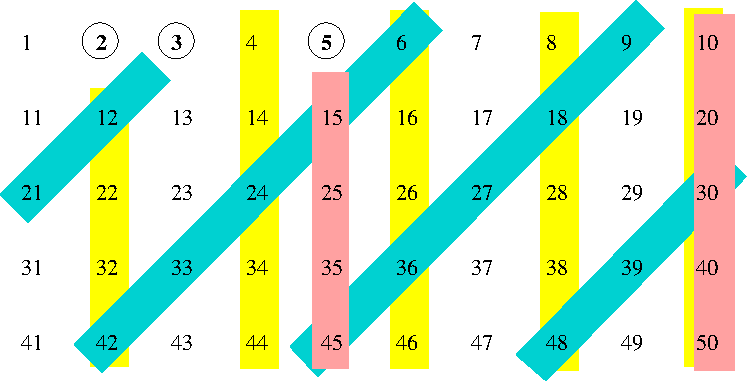
\includegraphics{./Eratosthenes.pdf}%
\end{picture}%
\setlength{\unitlength}{3947sp}%
%
\begingroup\makeatletter\ifx\SetFigFont\undefined%
\gdef\SetFigFont#1#2#3#4#5{%
  \reset@font\fontsize{#1}{#2pt}%
  \fontfamily{#3}\fontseries{#4}\fontshape{#5}%
  \selectfont}%
\fi\endgroup%
\begin{picture}(5970,3042)(1632,-3011)
\end{picture}%

\caption[The sieve of Eratosthenes.]{The first three stages in the %
sieve of Eratosthenes.  What is the smallest composite number that %
hasn't been crossed off?}
\label{fig:sieve} 
\end{figure}

It is interesting to note that the sieve gives us a means of finding
all the primes up to $p^2$ by using the primes up to (but not
including) $p$.  For
example, to find all the primes less than $13^2 = 169$, we need only
use $2, 3, 5, 7$ and $11$ in the sieve.

Despite the fact that one can find primes using this simple 
mechanical method, the way that prime numbers are distributed
amongst the integers is very erratic.  Nearly any statement that
purports to show some regularity in the distribution of the 
primes will turn out to be false.  Here are two such false
conjectures regarding prime numbers.

\begin{conj} \label{conj:ferm}
Whenever $p$ is a prime number, $2^p-1$ is also a prime.
\end{conj}

\begin{conj} \label{conj:poly}
The polynomial $x^2-31x+257$ evaluates to a prime number
whenever $x$ is a natural number.
\end{conj}

In the exercises for this section, you will be asked to
explore these statements further.  

Prime numbers act as multiplicative building blocks for the rest of
the integers.  When we disassemble an integer into its building blocks
we are finding the \index{prime factorization}\emph{prime factorization} 
of that number.  Prime
factorizations are unique.  That is, a number is either prime or it
has prime factors (possibly raised to various powers) that are
uniquely determined -- except that they may be re-ordered.

On the next page
is a table that contains all the primes that are less than 5000.
Study this table and discover the secret of its compactness!

\newpage


\renewcommand{\tabcolsep}{2.4pt}
\renewcommand{\arraystretch}{.63}
\addtolength{\lineskip}{-2pt}
{\small 
\hspace{-.5in}
\begin{tabular}{|lr|cccc|cccc|cccc|cccc|cccc|cccc|cccc|cccc|cccc|cccc|}
  \hline 
\rule{0pt}{10pt} & \bf T & \multicolumn{4}{c|}{\bf 0} & \multicolumn{4}{c|}{\bf 1} &
 \multicolumn{4}{c|}{\bf 2} & \multicolumn{4}{c|}{\bf 3} & \multicolumn{4}{c|}{\bf 4}
 & \multicolumn{4}{c|}{\bf 5} & \multicolumn{4}{c|}{\bf 6} &
 \multicolumn{4}{c|}{\bf 7} & \multicolumn{4}{c|}{\bf 8} & \multicolumn{4}{c|}{\bf 9}
 \\
\bf H & & & & & & & & & & & & & & & & & & & & & & & & & & & & & & & & & &
 & & & & & & & \\ \hline
\rule{0pt}{9pt}\bf 0 & & 2 & 3 & 5 & 7 & 1 & 3 & 7 & 9 & & 3 & & 9 & 1 & & 7 & & 1 & 3 & 7 & & & 3 & & 9 & 1 & & 7 & & 1 & 3 & & 9 & & 3 & & 9 & & & 7 & \\
\bf 1 & & 1 & 3 & 7 & 9 & & 3 & & & & & 7 & & 1 & & 7 & 9 & & & & 9 & 1 & & 7 & & & 3 & 7 & & & 3 & & 9 & 1 & & & & 1 & 3 & 7 & 9 \\
\bf 2 & & & & & & 1 & & & & & 3 & 7 & 9 & & 3 & & 9 & 1 & & & & 1 & & 7 & & & 3 & & 9 & 1 & & 7 & & 1 & 3 & & & & 3 & & \\
\bf 3 & & & & 7 & & 1 & 3 & 7 & & & & & & 1 & & 7 & & & & 7 & 9 & & 3 & & 9 & & & 7 & & & 3 & & 9 & & 3 & & 9 & & & 7 & \\
\bf 4 & & 1 & & & 9 & & & & 9 & 1 & & & & 1 & 3 & & 9 & & 3 & & 9 & & & 7 &
& 1 & 3 & 7 & & & & & 9 & & & 7 & & 1 & & & 9 \\ \hline
\rule{0pt}{9pt}\bf 5 & & & 3 & & 9 & & & & & 1 & 3 & & & & & & & 1 & & 7 & & & & 7 & & & 3 & & 9 & 1 & & 7 & & & & 7 & & & 3 & & 9 \\
\bf 6 & & 1 & & 7 & & & 3 & 7 & 9 & & & & & 1 & & & & 1 & 3 & 7 & & & 3 & & 9 & 1 & & & & & 3 & 7 & & & 3 & & & 1 & & & \\
\bf 7 & & 1 & & & 9 & & & & 9 & & & 7 & & & 3 & & 9 & & 3 & & & 1 & & 7 & & 1 & & & 9 & & 3 & & & & & 7 & & & & 7 & \\
\bf 8 & & & & & 9 & 1 & & & & 1 & 3 & 7 & 9 & & & & 9 & & & & & & 3 & 7 & 9 & & 3 & & & & & 7 & & 1 & 3 & 7 & & & & & \\
\bf 9 & & & & 7 & & 1 & & & 9 & & & & 9 & & & 7 & & 1 & & 7 & & & 3 & & & &
& 7 & & 1 & & 7 & & & 3 & & & 1 & & 7 & \\ \hline
\rule{0pt}{9pt}\bf 10 & & & & & 9 & & 3 & & 9 & 1 & & & & 1 & 3 & & 9 & & & & 9 & 1 & & & & 1 & 3 & & 9 & & & & & & & 7 & & 1 & 3 & 7 & \\
\bf 11 & & & 3 & & 9 & & & 7 & & & 3 & & 9 & & & & & & & & & 1 & 3 & & & & 3 & & & 1 & & & & 1 & & 7 & & & 3 & & \\
\bf 12 & & 1 & & & & & 3 & 7 & & & 3 & & 9 & 1 & & 7 & & & & & 9 & & & & 9 & & & & & & & 7 & 9 & & 3 & & 9 & 1 & & 7 & \\
\bf 13 & & 1 & 3 & 7 & & & & & 9 & 1 & & 7 & & & & & & & & & & & & & & 1 & & 7 & & & 3 & & & 1 & & & & & & & 9 \\
\bf 14 & & & & & 9 & & & & & & 3 & 7 & 9 & & 3 & & 9 & & & 7 & & 1 & 3 & & 9
& & & & & 1 & & & & 1 & 3 & 7 & 9 & & 3 & & 9 \\ \hline
\rule{0pt}{9pt}\bf 15 & & & & & & 1 & & & & & 3 & & & 1 & & & & & 3 & & 9 & & 3 & & 9 & & & 7 & & 1 & & & 9 & & 3 & & & & & 7 & \\
\bf 16 & & 1 & & 7 & 9 & & 3 & & 9 & 1 & & 7 & & & & 7 & & & & & & & & 7 & & & 3 & 7 & 9 & & & & & & & & & & 3 & 7 & 9 \\
\bf 17 & & & & & 9 & & & & & 1 & 3 & & & & 3 & & & 1 & & 7 & & & 3 & & 9 & & & & & & & 7 & & & 3 & 7 & 9 & & & & \\
\bf 18 & & 1 & & & & 1 & & & & & 3 & & & 1 & & & & & & 7 & & & & & & 1 & & 7 & & 1 & 3 & 7 & 9 & & & & 9 & & & & \\
\bf 19 & & 1 & & 7 & & & 3 & & & & & & & 1 & 3 & & & & & & 9 & 1 & & & & & &
& & & 3 & & 9 & & & 7 & & & 3 & 7 & 9 \\ \hline
\rule{0pt}{9pt}\bf 20 & & & 3 & & & 1 & & 7 & & & & 7 & 9 & & & & 9 & & & & & & 3 & & & & 3 & & 9 & & & & & 1 & 3 & 7 & 9 & & & & 9 \\
\bf 21 & & & & & & 1 & 3 & & & & & & 9 & 1 & & 7 & & 1 & 3 & & & & 3 & & & 1 & & & & & & & 9 & & & & & & & & \\
\bf 22 & & & 3 & 7 & & & 3 & & & 1 & & & & & & 7 & 9 & & 3 & & & 1 & & & & & & 7 & 9 & & 3 & & & 1 & & 7 & & & 3 & 7 & \\
\bf 23 & & & & & 9 & 1 & & & & & & & & & 3 & & 9 & 1 & & 7 & & 1 & & 7 & & & & & & 1 & & 7 & & 1 & 3 & & 9 & & 3 & & 9 \\
\bf 24 & & & & & & 1 & & 7 & & & 3 & & & & & 7 & & 1 & & 7 & & & & & 9 & & &
7 & & & 3 & 7 & & & & & & & & & \\ \hline
\rule{0pt}{9pt}\bf 25 & & & 3 & & & & & & & 1 & & & & 1 & & & 9 & & 3 & & 9 & 1 & & 7 & & & & & & & & & 9 & & & & & 1 & 3 & & \\
\bf 26 & & & & & 9 & & & 7 & & 1 & & & & & 3 & & & & & 7 & & & & 7 & 9 & & 3 & & & 1 & & 7 & & & 3 & 7 & 9 & & 3 & & 9 \\
\bf 27 & & & & 7 & & 1 & 3 & & 9 & & & & 9 & 1 & & & & 1 & & & 9 & & 3 & & & & & 7 & & & & 7 & & & & & 9 & 1 & & 7 & \\
\bf 28 & & 1 & 3 & & & & & & 9 & & & & & & 3 & 7 & & & 3 & & & 1 & & 7 & & 1 & & & & & & & 9 & & & 7 & & & & 7 & \\
\bf 29 & & & 3 & & 9 & & & 7 & & & & 7 & & & & & 9 & & & & & & 3 & 7 & & & 3
& & 9 & 1 & & & & & & & & & & & 9 \\ \hline
\rule{0pt}{9pt}\bf 30 & & 1 & & & & 1 & & & 9 & & 3 & & & & & 7 & & 1 & & & 9 & & & & & 1 & & 7 & & & & & 9 & & 3 & & 9 & & & & \\
\bf 31 & & & & & 9 & & & & 9 & 1 & & & & & & 7 & & & & & & & & & & & 3 & 7 & 9 & & & & & 1 & & 7 & & 1 & & & \\
\bf 32 & & & 3 & & 9 & & & 7 & & 1 & & & 9 & & & & & & & & & 1 & 3 & 7 & 9 & & & & & 1 & & & & & & & & & & & 9 \\
\bf 33 & & 1 & & 7 & & & 3 & & 9 & & 3 & & 9 & 1 & & & & & 3 & 7 & & & & & 9 & 1 & & & & 1 & 3 & & & & & & 9 & 1 & & & \\
\bf 34 & & & & 7 & & & 3 & & & & & & & & 3 & & & & & & 9 & & & 7 & & 1 & 3 &
7 & 9 & & & & & & & & & 1 & & & 9 \\ \hline
\rule{0pt}{9pt}\bf 35 & & & & & & 1 & & 7 & & & & 7 & 9 & & 3 & & 9 & 1 & & 7 & & & & 7 & 9 & & & & & 1 & & & & 1 & 3 & & & & 3 & & \\
\bf 36 & & & & 7 & & & 3 & 7 & & & 3 & & & 1 & & 7 & & & 3 & & & & & & 9 & & & & & 1 & 3 & 7 & & & & & & 1 & & 7 & \\
\bf 37 & & 1 & & & 9 & & & & 9 & & & 7 & & & 3 & & 9 & & & & & & & & & 1 & & 7 & 9 & & & & 9 & & & & & & 3 & 7 & \\
\bf 38 & & & 3 & & & & & & & 1 & 3 & & & & 3 & & & & & 7 & & 1 & 3 & & & & 3 & & & & & 7 & & 1 & & & 9 & & & & \\
\bf 39 & & & & 7 & & 1 & & 7 & 9 & & 3 & & 9 & 1 & & & & & 3 & 7 & & & & & &
& & 7 & & & & & & & & & 9 & & & & \\ \hline
\rule{0pt}{9pt}\bf 40 & & 1 & 3 & 7 & & & 3 & & 9 & 1 & & 7 & & & & & & & & & 9 & 1 & & 7 & & & & & & & 3 & & 9 & & & & & 1 & 3 & & 9 \\
\bf 41 & & & & & & 1 & & & & & & 7 & 9 & & 3 & & 9 & & & & & & 3 & 7 & 9 & & & & & & & 7 & & & & & & & & & \\
\bf 42 & & 1 & & & & 1 & & 7 & 9 & & & & 9 & 1 & & & & 1 & 3 & & & & 3 & & 9 & 1 & & & & 1 & 3 & & & & 3 & & 9 & & & 7 & \\
\bf 43 & & & & & & & & & & & & 7 & & & & 7 & 9 & & & & 9 & & & 7 & & & 3 & & & & 3 & & & & & & & 1 & & 7 & \\
\bf 44 & & & & & 9 & & & & & 1 & 3 & & & & & & & 1 & & 7 & & 1 & & 7 & & & 3
& & & & & & & 1 & 3 & & & & 3 & & \\ \hline
\rule{0pt}{9pt}\bf 45 & & & & 7 & & & 3 & 7 & 9 & & 3 & & & & & & & & & 7 & 9 & & & & & 1 & & 7 & & & & & & & 3 & & & 1 & & 7 & \\
\bf 46 & & & 3 & & & & & & & 1 & & & & & & 7 & 9 & & 3 & & 9 & 1 & & 7 & & & 3 & & & & 3 & & 9 & & & & & 1 & & & \\
\bf 47 & & & 3 & & & & & & & 1 & 3 & & 9 & & 3 & & & & & & & 1 & & & 9 & & & & & & & & & & 3 & 7 & 9 & & 3 & & 9 \\
\bf 48 & & 1 & & & & & 3 & 7 & & & & & & 1 & & & & & & & & & & & & 1 & & & & 1 & & 7 & & & & & 9 & & & & \\
\bf 49 & & & 3 & & 9 & & & & 9 & & & & & 1 & 3 & 7 & & & 3 & & & 1 & & 7 & &
& & 7 & 9 & & 3 & & & & & 7 & & & 3 & & 9 \\ \hline
\end{tabular}
}

\addtolength{\lineskip}{2pt}
\renewcommand{\arraystretch}{1}

\clearpage

\noindent{\large \bf Exercises --- \thesection\ }

\begin{enumerate}

\item Find the prime factorizations of the following integers.

  \begin{enumerate}
  \item 105
  \item 414
  \item 168
  \item 1612
  \item 9177
  \end{enumerate}

\hint{Divide out the obvious factors in order to reduce the complexity of the remaining problem. The first number is divisible by 5. The next three are all even. Recall that a number is divisible by 3 if and only if the sum of its digits is divisible by 3.
}

\item Use the sieve of Eratosthenes to find all prime numbers
up to 100.

\begin{tabular}{cccccccccc}
\rule{14pt}{0pt} & \rule{14pt}{0pt} & \rule{14pt}{0pt} &
\rule{14pt}{0pt} & \rule{14pt}{0pt} & \rule{14pt}{0pt} & 
\rule{14pt}{0pt} & \rule{14pt}{0pt} & \rule{14pt}{0pt} &
\rule{14pt}{0pt} \\
 1 & 2 & 3 & 4 & 5 & 6 & 7 & 8 & 9 & 10 \\
 11 & 12 & 13 & 14 & 15 & 16 & 17 & 18 & 19 & 20 \\
 21 & 22 & 23 & 24 & 25 & 26 & 27 & 28 & 29 & 30 \\
 31 & 32 & 33 & 34 & 35 & 36 & 37 & 38 & 39 & 40 \\
 41 & 42 & 43 & 44 & 45 & 46 & 47 & 48 & 49 & 50 \\
 51 & 52 & 53 & 54 & 55 & 56 & 57 & 58 & 59 & 60 \\ 
 61 & 62 & 63 & 64 & 65 & 66 & 67 & 68 & 69 & 70 \\
 71 & 72 & 73 & 74 & 75 & 76 & 77 & 78 & 79 & 80 \\
 81 & 82 & 83 & 84 & 85 & 86 & 87 & 88 & 89 & 90 \\
 91 & 92 & 93 & 94 & 95 & 96 & 97 & 98 & 99 & 100
\end{tabular}

\hint{The primes used in this instance of the sieve are just 2, 3, 5 and 7. Any number less than 100 that isn't a multiple of 2, 3, 5 or 7 will not be crossed off during the sieving process. If you're still unclear about the process, try a web search for {\tt "Sieve of Eratosthenes" +applet}, there are several interactive applets that will help you to understand how to sieve.
}

\item What would be the largest prime one would sieve with
in order to find all primes up to 400?

\hint{Remember that if a number factors into two multiplicands, the smaller of them will be less than the square root of the original number.}

\wbvfill

\workbookpagebreak

\item Characterize the prime factorizations of numbers that are
  perfect squares.

\wbvfill

\hint{It might be helpful to write down a bunch of examples. Think about how the prime factorization of a number gets transformed when we square it.}

\textbookpagebreak

\item Complete the following table which is related to 
\ifthenelse{\boolean{InTextBook}}{Conjecture~\ref{conj:ferm}}{the conjecture that whenever $p$ is a prime number, $2^p-1$ is also a prime}.

\begin{tabular}{c|c|c|c}
$p$ & $2^p-1$ & prime? & factors \\ \hline
2 & 3 & yes & 1 and 3 \\
3 & 7 & yes & 1 and 7 \\
5 & 31 & yes &  \\
7 & 127   &     &    \\
11 &   &     &    
\end{tabular}

\hint{
You'll need to determine if $2^{11}-1 = 2047$ is prime or not. If you never figured out how to read the table of primes on page 15, here's a hint: If 2047 was a prime there would be a 7 in the cell at row 20, column 4.

A quick way to find the factors of a not-too-large number is to use the "table" feature of your graphing calculator. If you enter y1=2047/X and select the table view (2ND GRAPH). Now, just scan down the entries until you find one with nothing after the decimal point. That's an X that evenly divides 2047!

An even quicker way is to type {\tt factor(2047)} in Sage.
}



\hintspagebreak

\item Find a counterexample for \ifthenelse{\boolean{InTextBook}}{Conjecture~\ref{conj:poly}}{the conjecture that $x^2-31x+257$ evaluates to a prime number
whenever $x$ is a natural number}.

\wbvfill

\hint{Part of what makes the "prime-producing-power" of that polynomial impressive is that it gives each prime twice -- once on the descending arm of the parabola and once on the ascending arm. In other words, the polynomial gives prime values on a set of contiguous natural numbers {0,1,2, ..., N} and the vertex of the parabola that is its graph lies dead in the middle of that range. You can figure out what N is by thinking about the other end of the range: (-1)2 + 31 · (-1) + 257 = 289 (289 is not a prime, you should recognize it as a perfect square.)}

\item Use the second definition of ``prime'' to see that $6$ is
not a prime.  In other words, find two numbers (the $a$ and $b$ 
that appear in the definition) such that $6$ is not a factor of
either, but {\em is} a factor of their product.

\wbvfill

\hint{Well, we know that 6 really isn't a prime... Maybe its factors enter into this somehow\ldots}

\item Use the second definition of ``prime'' to show that $35$ is
not a prime.

\wbvfill

\hint{How about $a=2\cdot5$ and $b=3\cdot7$.  Now you come up with a different pair!}

\workbookpagebreak

\item A famous conjecture that is thought to be true (but
for which no proof is known) is the  \index{Twin Prime conjecture}
Twin Prime conjecture.
A pair of primes is said to be twin if they differ by 2.
For example, 11 and 13 are twin primes, as are 431 and 433.
The Twin Prime conjecture states that there are an infinite
number of such twins.  Try to come up with an argument as
to why 3, 5 and 7 are the only prime triplets.

\wbvfill

\hint{It has to do with one of the numbers being divisible by 3. (Why is this forced to be the case?) If that number isn't actually 3, then you know it's composite.}



\item Another famous conjecture, also thought to be true -- but
as yet unproved, is \index{Goldbach's conjecture}
Goldbach's conjecture.  Goldbach's conjecture
states that every even number greater than 4 is the sum of two odd
primes.  There is a function $g(n)$, known as the Goldbach function, defined
on the positive integers, that gives the number of different ways to 
write a given number as the sum of two odd primes.  For example $g(10) = 2$
since $10=5+5=7+3$.  Thus another version of Goldbach's conjecture
is that $g(n)$ is positive whenever $n$ is an even number greater than
4.

Graph $g(n)$ for $6 \leq n \leq 20$.

\wbvfill

\hint{If you don't like making graphs, a table of the values of g(n) would suffice. Note that we don't count sums twice that only differ by order. For example, 16 = 13+3 and 11+5 (and 5+11 and 3+13) but g(16)=2.}

\end{enumerate}


\newpage

\section{More scary notation}
\label{sec:scary}

It is often the case that we want to prove statements that
assert something is true for {\em every} element of a set.
For example, ``Every number has an additive inverse.''
You should note that the truth of that statement is relative,
it depends on what is meant by ``number.''  If we are talking
about natural numbers it is clearly false:  3's additive 
inverse isn't in the set under consideration.  If we are
talking about integers or any of the other sets we've considered,
the statement is true.  A statement that begins with the English
words ``every'' or ``all'' is called \index{universal quantification}
\emph{universally quantified}.
It is asserted that the statement holds for {\em everything} within
some universe.  It is probably clear that when we are making
statements asserting that a thing has an additive inverse, we 
are not discussing human beings or animals or articles of clothing --
we are talking about objects that it is reasonable to add together:
numbers of one sort or another.  When being careful -- and we should always
strive to be careful! -- it is important to make explicit what 
universe (known as the \index{universe of discourse}\emph{universe of discourse}) the objects
we are discussing come from.  Furthermore, we need to distinguish 
between statements that assert that everything in the universe of
discourse has some property, and statements that say something
about a few (or even just one) of the elements of our universe.
Statements of the latter sort are called \index{existential quantification}
\emph{existentially quantified}.

Adding to the glossary or translation lexicon we started earlier,
there are symbols which describe both these types of quantification.
The symbol $\forall$, an upside-down A, is used for universal
quantification, and is usually translated as ``for all.''  
The symbol $\exists$, a backwards E, is used for existential
quantification, it's translated as ``there is'' or ``there exists.''
Lets have a look at a mathematically precise sentence that captures
the meaning of the one with which we started this section.

\[ \forall x \in \Integers, \; \exists y \in \Integers, \; x+y=0. \]

Parsing this as we have done before with an English translation in 
parallel, we get:

\vspace{.2in}

\begin{tabular}{c|c|c}
\rule[-10pt]{0pt}{22pt} $\forall x$ & $\in \Integers$ & $\exists y$  \\ \hline
\rule[-6pt]{0pt}{22pt} For every number $x$ & in the set of integers &
there is a number $y$ \\
\end{tabular}

\vspace{.2in}

\begin{tabular}{c|c}
\rule[-10pt]{0pt}{22pt} $\in \Integers$ & $x+y=0$ \\ \hline
\rule[-6pt]{0pt}{22pt} in the integers  & having the property that
their sum is $0$. \\
\end{tabular}


\vspace{.2in}

\begin{exer} Which type of quantification do the following
statements have?
\begin{enumerate}
\item Every dog has his day.
\item Some days it's just not worth getting out of bed.
\item There's a party in {\em somebody's} dorm this Saturday.
\item There's someone for everyone.
\end{enumerate}
\end{exer}

A couple of the examples in the exercise above actually have two quantifiers
in them.  When there are two or more (different) quantifiers in a sentence
you have to be careful about keeping their order straight.  The following 
two sentences contain all the same elements except that the words that 
indicate quantification have been switched.  Do they have the same meaning?

\begin{quote}
For every student in James Woods High School, there is some item of
cafeteria food that they like to eat.
\end{quote}

\begin{quote}
There is some item of cafeteria food that every student in James Woods 
High School likes to eat.
\end{quote}

\newpage

\noindent{\large\bf Exercises --- \thesection\ }

\begin{enumerate}

\item How many quantifiers (and what sorts) are in the following sentence?

``Everybody has \emph{some} friend that thinks they know everything about 
a sport.''
  
\wbvfill

\hint{Four.}

\item The sentence ``Every metallic element is a solid at room temperature.'' 
is false.  Why?

\wbvfill

\hint{The chemical symbol for an element that is an exception is Hg which stands for "Hydro-argyrum" it is also known as "liquid silver" or "quick silver".}

\item The sentence ``For every pair of (distinct) real numbers there is 
another real number between them.'' is true.  Why?

\wbvfill

\hint{Think about this: is there any way to (using a formula) find a number that lies in between two other numbers?}

\item Write your own sentences containing four quantifiers.  One
sentence in which the quantifiers appear ($\forall \exists \forall \exists$)
and another in which they appear ($\exists \forall \exists \forall$).

\wbvfill

\hint{You're on your own here. Be inventive!}

\end{enumerate}



\newpage

\section{Definitions of elementary number theory}
\label{sec:num_thry}

\subsection{Even and odd}
\label{even_n_odd}

If you divide a number by 2 and it comes out even (i.e. with
no remainder) the number is said to be {\em even}.  So the 
{\em word} even is related to division.  It turns out that the
{\em concept} even is better understood through thinking about
multiplication.

\begin{defi}
An integer $n$ is {\em even} exactly when there is an integer $m$
such that $n = 2m$.
\end{defi}

You should note that there is a ``two-way street'' sort of quality
to this definition -- indeed with most, if not all, definitions.  If 
a number is even, then we are guaranteed the existence of another
integer half as big.  On the other hand, if we can show that another
integer half as big exists, then we know the original number is even.
This two-wayness means that the definition is what is known as a 
{\em biconditional}, a concept which we'll revisit in
Section~\ref{sec:impl}.  

A lot of people don't believe that $0$ should be counted as an even
number.  Now that we are armed with a precise definition, we can
answer this question easily.  Is there an integer $x$ such that
$0 = 2x$ ?  Certainly! let $x$ also be $0$.  (Notice that in the
definition, nothing was said about $m$ and $n$ being distinct from
one another.)  

An integer is {\em odd} if it isn't even.  That is, amongst integers,
there are only two possibilities: even or odd.  We can also define
oddness without reference to ``even.''

\begin{defi}
An integer $n$ is {\em odd} exactly when there is an integer $m$
such that $n = 2m + 1$.
\end{defi}


\subsection{Decimal and base-\emph{n} notation}\label{base-n}

You can also identify even numbers by considering their
decimal representation.  Recall that each digit in the 
decimal representation of a number has a value that depends
on its position.  For example, the number $3482$ really means
$3\cdot10^3 + 4\cdot10^2 + 8\cdot10^1 + 2\cdot10^0$.  This 
is also known as \index{place notation}place notation.  
The fact that we use the 
powers of 10 in our place notation is probably due to the
fact that most humans have 10 fingers.  It is possible to
use {\em any} number in place of 10.  In Computer Science there
are 3 other bases in common use: 2, 8 and 16 -- these are
known (respectively) as binary, octal and hexadecimal notation.
When denoting a number using some base other than 10, it is
customary to append a subscript indicating the base.
So, for example, $1011_2$ is binary notation meaning
$1\cdot2^3 + 0\cdot2^2 + 1\cdot2^1 + 1\cdot2^0$ or $8+2+1 = 11$.
No matter what base we are using, the rightmost digit of
the number multiplies the base raised to the $0$-th power.
Any number raised to the $0$-th power is 1, and the rightmost
digit is consequently known as the units digit.  We are now
prepared to give some statements that are equivalent to our
definition of even.  These statements truly don't deserve the
designation ``theorem,'' they are immediate consequences of the
definition.

\begin{thm}
An integer is {\em even} if the units digit in its decimal
representation is one of 0, 2, 4, 6 or 8.
\end{thm}

\begin{thm}
An integer is {\em even} if the units digit in its binary
representation is 0.
\end{thm}

\vspace{.5 in}

For certain problems it is natural to use some particular notational system.
For example, the
last theorem would tend to indicate that binary numbers are useful
in problems dealing with even and odd.  Given that there are many different 
notations that are available to us, it is obviously desirable to have 
means at our disposal for converting between them.  It is possible to 
develop general rules for converting a base-$a$ number to a base-$b$ 
number (where $a$ and $b$ are arbitrary) but it is actually more convenient 
to pick a ``standard'' base (and since we're human we'll use base-$10$) 
and develop methods for converting between an arbitrary base and the 
``standard'' one.  Imagine that in the not-too-distant future we need to 
convert some numbers from the base-$7$ system used by the Seven-lobed 
Amoebazoids from Epsilon Eridani III to the base-$12$ scheme favored 
by the Dodecatons of Alpha-Centauri IV.  We will need a procedure
for converting base-$7$ to base-$10$ and another procedure for converting 
from base-$10$ to base-$12$.  In the School House Rock episode 
``Little Twelve Toes'' they describe base-$12$
numeration in a way that is understandable for elementary school 
children -- the digits they use are 
$\{1, 2, 3, 4, 5, 6, 7, 8, 9, \delta, \epsilon \}$, the last two digits 
(which are pronounced ``dec'' and ``el'') are necessary since we need 
single symbols for the things we ordinarily denote using $10$ and $11$.

Converting from some other base to decimal is easy.  You just use the 
definition of place notation.  For example, to find what $451663_7$ 
represents in decimal, just write

\[ 4 \cdot 7^5 + 5 \cdot 7^4 + 1 \cdot 7^3 + 6 \cdot 7^2 + 6 \cdot 7 + 3 =  4 \cdot 16807 + 5 \cdot 2401 + 1 \cdot 343 + 6 \cdot 49 + 6 \cdot 7 + 3 = 79915. \] 

(Everything in the line above can be interpreted as a base-$10$ number, 
and no subscripts are necessary for base-$10$.)

Converting from decimal to some other base is harder.  There is an algorithm 
called ``repeated division'' that we'll explore a bit in the exercises 
for this section.  For the moment, just verify that 
$3\delta 2\epsilon 7_{12}$ is also a representation of the
number more conventionally written as 79915.

\subsection{Divisibility}
\label{div}

The notion of being even has an obvious generalization.  Suppose
we asked whether $3$ divided evenly into a given number.  Presumably
we could make a definition of what it meant to be {\em threeven}, but
rather than doing so (or engaging in any further punnery) we shall
instead move to a general definition.  We need a notation for the
situation when one number divides evenly into another.  There are
many ways to describe this situation in English, but essentially 
just one in ``math,''  we use a vertical bar -- {\em not} a fraction
bar.  Indeed the difference between this vertical bar and the 
fraction symbol (\rule{3pt}{0pt}$\divides$ versus $/$) needs to 
be strongly stressed.  The vertical bar
when placed between two numbers is a symbol which asks the question 
``Does the first number divide evenly (i.e. with no remainder) into 
the second?''  On the other hand the fraction bar asks you to actually
carry out some division.  The value of $2\divides 5$ is {\em false}, whereas
the value of $2/5$ is $.4$

As was the case in defining even, it turns out that it is best
to think of multiplication, not division, when making a formal
definition of this concept.  Given any two integers $n$ and $d$
we define the symbol \index{divisibility}$d\divides n$ by

\begin{defi}
$ d \divides n$ exactly when $\exists k \in \Integers$ such that $n = kd$.
\end{defi}

In spoken language the symbol $d \divides n$ can be translated in a variety 
of ways:

\begin{itemize}
\item $d$ is a divisor of $n$.
\item $d$ divides $n$ evenly.
\item $d$ is a factor of $n$.
\item $n$ is an integer multiple of $d$.
\end{itemize}

Although, by far the most popular way of expressing this concept is to just say ``$d$ divides $n$.''

\subsection{Floor and ceiling}
\label{floor}

Suppose there is an elevator with a capacity of 1300 pounds.  A large
group of men who all weigh about 200 pounds want to ascend in it.  How
many should ride at a time?  This is just a division problem, 1300/200
gives 6.5 men should ride together.  Well, obviously putting half a
person on an elevator is a bad idea -- should we just round-up and 
let 7 ride together?  Not if the 1300 pound capacity rating doesn't
have a safety margin!  This is an example of the kind of problem
in which the floor function is used.  The \index{floor function}
floor function takes a real number as input and returns the next 
lower integer.

Suppose after a party we have 43 unopened bottles of beer.  We'd like
to store them in containers that hold 12 bottles each.  How many 
containers will we need?  Again, this is simply a division problem --
$43/12 = 3.58\overline{333}$.  So we need 3 boxes and another 
7 twelfths of a box.  Obviously we really need 4 boxes -- at least one
will have some unused space in it.  In this sort of situation
we're dealing with the \index{ceiling function}ceiling function.  
Given a real number, the ceiling function rounds it up to the 
next integer.

Both of these functions are denoted using symbols that look very
much like absolute value bars.  The difference lies in some 
small horizontal strokes.

If $x$ is a real number, its floor is denoted $\lfloor x \rfloor$,
and its ceiling is denoted $\lceil x \rceil$.  Here are the 
formal definitions:

\begin{defi}
$y = \lfloor x \rfloor$ exactly when $y \in \Integers$ and 
$y \leq x < y+1$.
\end{defi}

\begin{defi}
$y = \lceil x \rceil$ exactly when $y \in \Integers$ and 
$y-1 < x \leq y$.
\end{defi}

Basically, the definition of floor says that $y$ is an integer
that is less than or equal to $x$, but $y+1$ definitely exceeds $x$.
The definition of ceiling can be paraphrased similarly.


\subsection{Div and mod}
\label{div/mod}

In the next section we'll discuss the so-called division algorithm --
this may be over-kill since you certainly already know how to do
division!  Indeed, in the U.S., long division is usually first studied
in the latter half of elementary school, and division problems that
don't involve a remainder may be found as early as the first grade.
Nevertheless, we're going to discuss this process in sordid detail
because it gives us a good setting in which to prove relatively easy
statements.  Suppose you are setting-up a long division problem in
which the integer $n$ is being divided by a positive divisor $d$.
(If you want to divide by a negative number, just divide by the
corresponding positive number and then throw an extra minus sign 
on at the end.)

\centerline{ \begin{tabular}{cc}
 & q \\ 
 d & \begin{tabular}{|c} \hline 
     \rule{8pt}{0pt} n \rule{8pt}{0pt} 
     \end{tabular}  \\
 & $\vdots$ \\ \cline{2-2}
 & r \\
\end{tabular} }

Recall that the answer consists of two parts, a {\em quotient} $q$,
and a {\em remainder} $r$.  Of course, $r$ may be zero, but also, the
largest $r$ can be is $d-1$.  The assertion that this answer uniquely
exists is known as the \index{quotient-remainder theorem}
\emph{quotient-remainder theorem}:

\begin{thm} \label{quo-rem}
Given integers $n$ and $d>0$, there are unique integers $q$ and $r$ such
that $n = qd + r$ and $ 0 \leq r < d$.
\end{thm}

The words ``div'' and ``mod'' that appear in the title of this
subsection provide mathematical shorthand for $q$ and $r$.   Namely,
``$n \bmod d$'' is a way of expressing the remainder $r$, and ``$n
\tdiv d$'' is a way of expressing the quotient $q$. 

If two integers, $m$ and $n$, leave the same remainder when you
divide them by $d$, we say that they are \index{congruence}
\emph{congruent modulo $d$}.
One could express this by writing $n \bmod d = m \bmod d$, but usually
we adopt a shorthand notation

\[ n \equiv m \pmod{d}. \]

If one is in a context in which it is completely clear what $d$ is, it's
acceptable to just write $n \equiv m$.

The ``mod'' operation is used quite a lot in mathematics.  When we do 
computations modulo some number $d$, (this is known as ``modular arithmetic''
or, sometimes, ``clock arithmetic'') some very nice properties of ``mod''
come in handy:

\[ x + y \bmod d = ( x \bmod d + y \bmod d ) \bmod d \]

\noindent and

\[ x \cdot y \bmod d = ( x \bmod d \cdot y \bmod d ) \bmod d. \] 

These rules mean that we can either do the operations first, then 
reduce the answer $\bmod\; d$ or we can do the reduction $\bmod\; d$ 
first and then do the operations (although we may have to do one 
more round of reduction $\bmod\; d$).

For example, if we are working $\bmod\; 10$, and want to compute 
$87 \cdot 96 \bmod\; 10$, we can instead just compute $7 \cdot 6 \bmod\; 10$,
which is $2$.

\subsection{Binomial coefficients}
\label{binom_coeff}

A ``binomial'' is a polynomial with 2 terms, for example $x+1$ or $a+b$.
The numbers that appear as the coefficients when one raises a binomial
to some power are -- rather surprisingly -- known as 
\index{binomial coefficients} binomial coefficients.

Let's have a look at the first several powers of $a+b$.

\begin{gather*}
(a+b)^0 = 1 \\
(a+b)^1 = a+b \\
(a+b)^2 = a^2 + 2ab + b^2 \\
\end{gather*} 

To go much further than the second power requires a bit of work,
but try the following

\begin{exer}
Multiply $(a+b)$ and $(a^2 + 2ab + b^2)$ in order to determine $(a+b)^3$.
If you feel up to it, multiply $(a^2 + 2ab + b^2)$ times itself in order
to find $(a+b)^4$.
\end{exer}

Since we're interested in the coefficients of these polynomials, it's important
to point out that if no coefficient appears in front of a term that means the
coefficient is 1.

These binomial coefficients can be placed in an arrangement known as
\index{Pascal's triangle} \index{Blaise Pascal} Pascal's triangle
\footnote{This triangle was actually known well before Blaise Pascal %
began to study it, but it carries his name today.}, which
provides a convenient way to calculate small binomial coefficients

\begin{figure}[!hbt]
\begin{center}
\begin{tabular}{ccccccccc}
 & & & & 1 & & & & \\
 & & & 1 & & 1 & & & \\
 & & 1 &  & 2 &  & 1 & & \\ 
 & 1 & & 3 & & 3 & & 1 & \\
1 & & 4 & & 6 & & 4 & & 1 \\
\end{tabular}
\end{center}

\vspace{.2in}

\caption[Pascal's triangle.]{The first $5$ rows of Pascal's triangle (which are numbered 0 through 4 \ldots).}
\label{fig:pascal}
\end{figure}

Notice that in the triangle there is a border on both sides containing
1's and that the numbers on the inside of the triangle are the sum of the
two numbers above them.  You can use these facts to extend the triangle.

\begin{exer}
Add the next two rows to the Pascal triangle in Figure~\ref{fig:pascal}.
\end{exer}

Binomial coefficients are denoted using a somewhat strange looking
symbol.  The number in the $k$-th position in row number $n$ of
the triangle is denoted $\displaystyle \binom{n}{k}$.  This looks 
a little like a fraction, but the fraction bar is missing.  Don't
put one in!  It's \emph{supposed} to be missing.  In spoken English
you say ``$n$ choose $k$'' when you encounter the symbol $\displaystyle \binom{n}{k}$. 

There is a formula for the binomial coefficients -- which is nice.  Otherwise
we'd need to complete a pretty huge Pascal triangle in order to compute
something like $\displaystyle \binom{52}{5}$.  The formula involves 
\index{factorials} factorial notation.  Just to be sure we are 
all on the same page, we'll define factorials before proceeding.

The symbol for factorials is an exclamation point following a number.
This is just a short-hand for expressing the
product of all the numbers up to a given one.
For example $7!$ means $1\cdot 2\cdot 3\cdot 4\cdot 5\cdot 6\cdot 7$.
Of course, there's really no need to write the initial $1$ --- also,
for some reason people usually write the product in decreasing order
($7! = 7 \cdot 6 \cdot 5 \cdot 4 \cdot 3 \cdot 2)$.

The formula for a binomial coefficient is 

\[ \binom{n}{k} = \frac{n!}{k! \cdot (n-k)!}. \]

For example

\[ \binom{5}{3} = \frac{5!}{3! \cdot (5-3)!} = \frac{1\cdot 2\cdot 3\cdot 4\cdot 5}{(1\cdot 2\cdot 3) \cdot (1\cdot 2)} = 10. \]

A slightly more complicated example (and one that gamblers are fond of) 
is

\begin{gather*} 
\binom{52}{5} = \frac{52!}{5! \cdot (52-5)!} 
 = \frac{1\cdot 2\cdot 3\cdot \cdots 52}{(1\cdot 2\cdot 3 \cdot 4 \cdot 5) \cdot (1\cdot 2 \cdot 3\cdot \cdots 47)}\\
 = \frac{48 \cdot 49 \cdot 50 \cdot 51 \cdot 52}{1\cdot 2\cdot 3 \cdot 4 \cdot 5} = 2598960.
\end{gather*}

The reason that a gambler might be interested in the number we just calculated
is that binomial coefficients do more than just give us the coefficients in the
expansion of a binomial.  They also can be used to compute how many ways one
can choose a subset of a given size from a set.  Thus $\binom{52}{5}$ is the
number of ways that one can get a 5 card hand out of a deck of 52 cards.  

\begin{exer}
There are seven days in a week.  In how many ways can one choose a set
of three days (per week)?
\end{exer}

\newpage

\noindent{\large\bf Exercises --- \thesection\ }

\begin{enumerate}

\item An integer $n$ is \index{doubly-even} \emph{doubly-even} 
if it is even, and the integer $m$ guaranteed to exist because 
$n$ is even is itself even.  Is 0 doubly-even?  What are the 
first 3 positive, doubly-even integers?

\wbvfill

\hint{Answers: yes, 0,4 and 8.}

\item Dividing an integer by two has an interesting interpretation
when using binary notation: simply shift the digits to the right.
Thus, $22 = 10110_2$ when divided by two gives $1011_2$ which is
$8+2+1=11$.  How can you recognize a doubly-even integer from
its binary representation?

\wbvfill

\hint{Even numbers have a zero in their units place. What digit must also be zero in a doubly-even number's binary representation?}

\item The \index{octal representation} \emph{octal} representation 
of an integer uses powers of 8 in place notation.  The digits of an 
octal number run from 0 to 7, one never sees 8's or 9's.  How would 
you represent 8 and 9 as octal numbers?  What octal number comes 
immediately after $777_8$?  What (decimal) number is $777_8$?

\wbvfill

\workbookpagebreak

\hint{Eight is $10_8$, nine is $11_8$. The point of asking questions about $777$, is that (in octal) $7$ is the digit that is analogous to $9$ in base-$10$. Thus $777_8$ is something like $999_{10}$ in that the number following both of them is written $1000$ (although $1000_8$ and $1000_{10}$ are certainly not equal!)}

\hintspagebreak

\item One method of converting from decimal to some other base is
called \index{repeated division algorithm} \emph{repeated division}.  
One divides the number by the base
and records the remainder -- one then divides the quotient obtained
by the base and records the remainder.  Continue dividing the 
successive quotients by the base until the quotient is smaller than
the base.  Convert 3267 to base-7 using repeated division.  Check 
your answer by using the meaning of base-7 place notation.  (For
example $54321_7$ means $5\cdot7^4 + 4\cdot7^3 + 3 \cdot7^2 +
2\cdot7^1 + 1\cdot7^0$.)

\wbvfill

\hint{It is helpful to write something of the form $n = qd+r$ at each stage. The first two stages should look like

\[ 3267 \; = \; 466 \cdot 7 + 5 \]

\[ 466 \; = \; 66 \cdot 7 + 4 \]

you do the rest\ldots
}

\item State a theorem about the octal representation of even numbers.

\wbvfill

\hint{One possibility is to mimic the result for base-10 that an even number always ends in 0,2,4,6 or 8.}

\item In hexadecimal (base-16) notation one needs 16 ``digits,'' the
  ordinary digits are used for 0 through 9, and the letters A through
  F are used to give single symbols for 10 through 15.  The first  32
  natural number in hexadecimal are:
  1,2,3,4,5,6,7,8,9,A,B,C,D,E,F,10,11,12,13,14,15,16,\newline 17,18,19,1A,
  1B,1C,1D,1E,1F,20. 

  Write the next 10 hexadecimal numbers after $AB$.

  Write the next 10 hexadecimal numbers after $FA$.

\hint{As a check, the tenth number after AB is B5.\newline
The tenth hexadecimal number after FA is 104.}

\wbvfill

\workbookpagebreak

\item For conversion between the three bases used most often in 
Computer Science we can take binary as the ``standard'' base and 
convert using a table look-up.  Each octal digit will correspond 
to a binary triple, and each hexadecimal digit will correspond to 
a 4-tuple of binary numbers.  Complete the following tables.  
(As a check, the 4-tuple next to $A$ in the table for
hexadecimal should be 1010 -- which is nice since $A$ 
is really 10 so if you read that as ``ten-ten'' it is a good 
aid to memory.)

\begin{center}
\begin{tabular}{ccc}
\begin{tabular}{|c|c|} \hline
octal & binary \\ \hline \hline
\rule{0pt}{14pt} 0 & 000 \\ \hline
\rule{0pt}{14pt} 1 & 001 \\ \hline
\rule{0pt}{14pt} 2 & \\ \hline
\rule{0pt}{14pt} 3 & \\ \hline
\rule{0pt}{14pt} 4 & \\ \hline
\rule{0pt}{14pt} 5 & \\ \hline
\rule{0pt}{14pt} 6 & \\ \hline
\rule{0pt}{14pt} 7 & \\ \hline
\end{tabular}
 & \rule{72pt}{0pt} &
\begin{tabular}{|c|c|} \hline
hexadecimal & binary \\ \hline \hline
\rule{0pt}{14pt} 0 & 0000 \\ \hline
\rule{0pt}{14pt} 1 & 0001 \\ \hline
\rule{0pt}{14pt} 2 & 0010 \\ \hline
\rule{0pt}{14pt} 3 & \\ \hline
\rule{0pt}{14pt} 4 & \\ \hline
\rule{0pt}{14pt} 5 & \\ \hline
\rule{0pt}{14pt} 6 & \\ \hline
\rule{0pt}{14pt} 7 & \\ \hline
\rule{0pt}{14pt} 8 & \\ \hline
\rule{0pt}{14pt} 9 & \\ \hline
\rule{0pt}{14pt} A & \\ \hline
\rule{0pt}{14pt} B & \\ \hline
\rule{0pt}{14pt} C & \\ \hline
\rule{0pt}{14pt} D & \\ \hline
\rule{0pt}{14pt} E & \\ \hline
\rule{0pt}{14pt} F & \\ \hline
\end{tabular}
\end{tabular}
\end{center}
 
\hint{

\vfill

This is just counting in binary. Remember the sanity check that the hexadecimal digit A is represented by 1010 in binary.  ($10_{10} \; = \; A_{16} \; = \; 1010_{2}$)

\vfill

}

\hintspagebreak
\workbookpagebreak
\textbookpagebreak

\item Use the tables from the previous problem to make the following conversions.

\begin{enumerate}
\item Convert $757_8$ to binary.
\item Convert $1007_8$ to hexadecimal.
\item Convert $100101010110_2$ to octal.
\item Convert $1111101000110101_2$ to hexadecimal.
\item Convert $FEED_{16}$ to binary.
\item Convert $FFFFFF_{16}$ to octal.
\end{enumerate}

\hint{Answers for the first three:
\[  757_8 = 111 101 111_2 \]
\[ 1007_8 = 001 000 000 111_2 = 0010 0000 0111_2 = 207_{16} \]
\[ 100 101 010 110_2 = 4526_8 \]
}

\item Try the following conversions between various number systems:

\begin{enumerate}
\item Convert $30$ (base 10) to binary.
\item Convert $69$ (base 10) to base 5.
\item Convert $1222_3$ to binary.
\item Convert $1234_7$ to base 10.
\item Convert $EEED_{15}$ to base 12. (Use $\{1, 2, 3 \ldots 9, d, e\}$ as the digits in base 12.)
\item Convert $678_{9}$ to hexadecimal.
\end{enumerate}

\item It is a well known fact that if a number is divisible by 3, then 3
  divides the sum of the (decimal) digits of that number.  Is this
  result true in base 7?  Do you think this result is true in {\em
  any} base? 
 
 \wbvfill
 
\hint{Might this effect have something to do with 10 being just one bigger than 9 (a multiple of 3)?}

\item Suppose that 340 pounds of sand must be placed into bags having
  a 50 pound capacity.  Write an expression using either floor or
  ceiling notation for the number of bags required.

\wbvfill

\hint{Seven 50 pound bags would hold 350 pounds of sand. They'd also be able to handle 340 pounds!}

\item True or false? 

\[ \left\lfloor \frac{n}{d}\right\rfloor < \left\lceil \frac{n}{d}\right\rceil \]
 
\noindent for all integers $n$ and $d>0$. Support your claim.

\wbvfill

\hint{You have to try a bunch of examples.  You should try to make sure the examples
you try cover all the possibilities.  The pairs that provide counterexamples (i.e. show the statement is false in general) are relatively sparse, so be systematic.}

\workbookpagebreak

\item What is the value of $\lceil\pi\rceil^{2}-\lceil\pi^{2}\rceil$?

\wbvfill

\hint{ $\pi^2 = 9.8696$ }



\item Assuming the symbols $n$,$d$,$q$ and $r$ have meanings as in the
  quotient-remainder theorem (\ifthenelse{\boolean{InTextBook}}{Theorem~\ref{quo-rem} on page \pageref{quo-rem}}{see page 29 of GIAM}).  Write
  expressions for $q$ and $r$, in terms of $n$ and $d$ using floor
  and/or ceiling notation.

\wbvfill

\hint{I just can't bring myself to spoil this one for you, you really need to work this out on your own. }

\textbookpagebreak

\item Calculate the following quantities:

\begin{enumerate}
\item \wbitemsep $3 \mod 5$
\item \wbitemsep $37 \mod 7$
\item \wbitemsep $1000001 \mod 100000$
\item \wbitemsep $6 \tdiv 6$
\item \wbitemsep $7 \tdiv 6$
\item \wbitemsep $1000001 \tdiv 2$
\end{enumerate}

\hint{The even numbered ones are 2, 1, 500000.}

\hintspagebreak
\workbookpagebreak

\item Calculate the following binomial coefficients:

\begin{enumerate}
\item \wbitemsep $\binom{3}{0}$
\item \wbitemsep $\binom{7}{7}$
\item \wbitemsep $\binom{13}{5}$
\item \wbitemsep $\binom{13}{8}$
\item \wbitemsep $\binom{52}{7}$
\end{enumerate}

\hint{The even numbered ones are 1 and 1287. The TI-84 calculates binomial coefficients. The symbol used is {\tt nCr} (which is placed between the numbers -- i.e. it is an infix operator). You get {\tt nCr} as the 3rd item in the {\tt PRB} menu under {\tt MATH}. In sage the command is {\tt binomial(n,k)}.}

\item An ice cream shop sells the following flavors: chocolate, vanilla, 
strawberry, coffee, butter pecan, mint chocolate chip and raspberry.
How many different bowls of ice cream -- with three scoops -- can they make?  

\wbvfill

\hint{You're choosing three things out of a set of size seven\ldots}

\end{enumerate}


\newpage

\section[Some algorithms]{Some algorithms of elementary number theory}
\label{sec:alg}

An \index{algorithm}\emph{algorithm} is simply a set of clear 
instructions for achieving
some task.  The Persian mathematician and astronomer
Al-Khwarizmi\footnote{Abu Ja'far Muhammad ibn Musa al-Khwarizmi} was a
scholar at the House of Wisdom in Baghdad who lived in the 8th and 9th
centuries A.D.   He is remembered for his algebra treatise \emph{Hisab
  al-jabr w'al-muqabala} from which we derive the very {\em word}
``algebra,'' and a text on the Hindu-Arabic numeration scheme.

\begin{quote}
Al-Khwarizmi also wrote a treatise on Hindu-Arabic numerals. The
Arabic text is lost but a Latin translation, {\em Algoritmi de numero
Indorum} (in English {\em Al-Khwarizmi on the Hindu Art of Reckoning}) gave
rise to the word algorithm deriving from his name in the
title.~\cite{HisMathArch} 
\end{quote}

While the study of algorithms is more properly a subject within
Computer Science, a student of Mathematics can derive considerable
benefit from it.  

There is a big difference between an algorithm description intended
for human consumption and one meant for a computer\footnote{The 
whole history of Computer Science could be
  described as the slow advance whereby computers have become  able to
  utilize more and more abstracted descriptions of algorithms. 
  Perhaps in the not-too-distant future machines will be capable of
  understanding instruction sets that currently require human interpreters.}.  
The two favored human-readable forms for describing
algorithms are \index{pseudocode} pseudocode and \index{flowchart} 
flowcharts.  The former is text-based
and the latter is visual.  There are many different modules from which
one can build algorithmic structures: for-next loops, do-while loops, if-then
statements, goto statements, switch-case structures, etc.   We'll use
a minimal subset of the choices available.

\begin{itemize}
\item Assignment statements
\item If-then control statements
\item Goto statements
\item Return
\end{itemize}

We take the view that an algorithm is something like a function, it
takes for its input a list of parameters that describe a particular
case of some general problem, and produces as its output a solution to
that problem.  (It should be noted that there are other possibilities
-- some programs require that the variable in which the output is to
be placed be handed them as an input parameter, others have no
specific output, their purpose is achieved as a side-effect.)  The
intermediary between input and output is the algorithm instructions
themselves and a set of so-called local variables which are used much
the way scrap paper is used in a hand calculation -- intermediate
calculations are written on them, but they are tossed aside once the
final answer has been calculated.

Assignment statements allow us to do all kinds of arithmetic
operations (or rather to think of these types of operations as being
atomic.)  In actuality even a simple procedure like adding two numbers
requires an algorithm of sorts, we'll avoid such a fine level of
detail.  Assignments consist of evaluating some (possibly quite
complicated) formula in the inputs and local variables and assigning
that value to some local variable.  The two uses of the phrase ``local
variable''  in the previous sentence do not need to be distinct, thus
$x = x + 1$ is a perfectly legal assignment. 

If-then control statements are decision makers.  They first calculate
a Boolean expression (this is just a fancy way of saying something
that is either {\tt true} or {\tt false}), and send program flow to 
different locations depending on that result.  A small example will
serve as an illustration.  Suppose that in the body of an algorithm we
wish to check if 2 variables, $x$ and $y$ are equal, and if they are,
increment $x$ by 1.  This is illustrated in Figure~\ref{fig:if-then}
both in pseudocode and as a flowchart. 

\begin{figure}[!hbt] 
\begin{tabular}{ccc} 
\begin{picture}(0,0)%
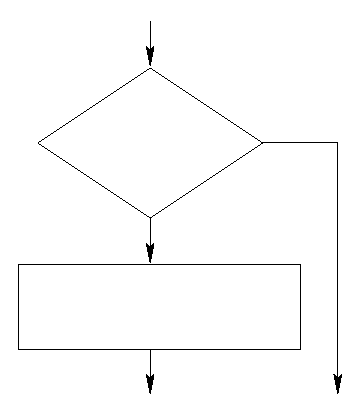
\includegraphics{figures/if-then_flowchart.pdf}%
\end{picture}%
\setlength{\unitlength}{3947sp}%
%
\begingroup\makeatletter\ifx\SetFigFont\undefined%
\gdef\SetFigFont#1#2#3#4#5{%
  \reset@font\fontsize{#1}{#2pt}%
  \fontfamily{#3}\fontseries{#4}\fontshape{#5}%
  \selectfont}%
\fi\endgroup%
\begin{picture}(2852,3302)(1200,-3662)
\put(2476,-2236){\makebox(0,0)[lb]{\smash{{\SetFigFont{12}{14.4}{\familydefault}{\mddefault}{\updefault}{\color[rgb]{0,0,0}Yes}%
}}}}
\put(3376,-1411){\makebox(0,0)[lb]{\smash{{\SetFigFont{12}{14.4}{\familydefault}{\mddefault}{\updefault}{\color[rgb]{0,0,0}No}%
}}}}
\put(1726,-2836){\makebox(0,0)[lb]{\smash{{\SetFigFont{12}{14.4}{\familydefault}{\mddefault}{\updefault}{\color[rgb]{0,0,0}Let $x = x + 1$.}%
}}}}
\put(1801,-1561){\makebox(0,0)[lb]{\smash{{\SetFigFont{12}{14.4}{\familydefault}{\mddefault}{\updefault}{\color[rgb]{0,0,0}Is $x$ equal to $y$?}%
}}}}
\end{picture}%
 
 & \hspace{1in} &
\begin{minipage}[b]{.3\textwidth}
\tt If $x=y$ then \\
\rule{15pt}{0pt}  $x=x+1$ \\
End If \\
\rule{30pt}{0pt} \vdots\\
\\
\\
\end{minipage} \\
\end{tabular}
\caption{A small example in pseudocode and as a flowchart}
\label{fig:if-then}
\end{figure}

Notice the use of indentation in the pseudocode example to indicate
the statements that are executed if the Boolean expression is true.
These examples also highlight the difference between the two senses 
that the word ``equals'' (and the symbol $=$) has.  In the Boolean
expression the sense is that of {\em testing} equality, in the
assignment statements (as the name implies) an {\em assignment} is
being made.  In many programming languages this distinction is made
explicit, for instance in the C language equality testing is done via
the symbol ``=='' whereas assignment is done using a single equals
sign ($=$).  In Mathematics the equals sign usually indicates equality
testing, when the assignment sense is desired the word ``let'' will
generally precede the equality.

While this brief introduction to the means of notating algorithms is by no
means complete, it is hopefully sufficient for our purpose which is
solely to introduce two algorithms that are important in elementary
number theory.  The \index{division algorithm} division algorithm, 
as presented here, is simply
an explicit version of the process one follows to calculate a quotient
and remainder using long division.  The procedure we give is unusually
inefficient -- with very little thought one could devise an algorithm
that would produce the desired answer using many fewer operations --
however the main point here is purely to show that division can be
accomplished by essentially mechanical means.  The Euclidean algorithm
is far more interesting both from a theoretical and a practical
perspective.  The Euclidean algorithm computes the greatest common
divisor (gcd) of two integers.  The gcd of of two numbers $a$ and $b$
is denoted $\gcd{a}{b}$ and is the largest integer that divides both
$a$ and $b$ evenly.   

A pseudocode outline of the division algorithm is as follows:
\medskip

\begin{center}
\begin{minipage}[b]{.5\textwidth}
\tt Algorithm: Division\\
Inputs: integers $n$ and $d$.\\
Local variables: $q$ and $r$.\\
\\
Let $q = 0$. \\
Let $r = n$. \\
Label 1.\\
If $r < d$ then\\
\rule{15pt}{0pt} Return $q$ and $r$.\\
End If\\
Let $q = q + 1$.\\
Let $r = r - d$.\\
Goto 1. \\
\end{minipage}
\end{center}

This same algorithm is given in flowchart form in
Figure~\ref{fig:div_alg}.

\begin{figure}[!hbt]
\begin{center}
\begin{picture}(0,0)%
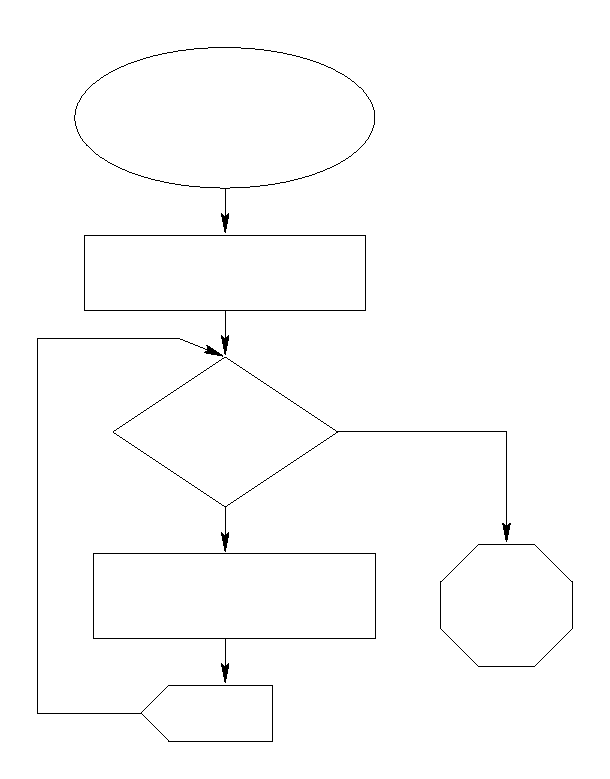
\includegraphics{./div_alg_flowchart.pdf}%
\end{picture}%
\setlength{\unitlength}{3947sp}%
%
\begingroup\makeatletter\ifx\SetFigFont\undefined%
\gdef\SetFigFont#1#2#3#4#5{%
  \reset@font\fontsize{#1}{#2pt}%
  \fontfamily{#3}\fontseries{#4}\fontshape{#5}%
  \selectfont}%
\fi\endgroup%
\begin{picture}(4877,6227)(900,-6287)
\put(2189,-4747){\makebox(0,0)[lb]{\smash{{\SetFigFont{12}{14.4}{\familydefault}{\mddefault}{\updefault}{\color[rgb]{0,0,0}Let $r = r - d$.}%
}}}}
\put(1876,-886){\makebox(0,0)[lb]{\smash{{\SetFigFont{12}{14.4}{\familydefault}{\mddefault}{\updefault}{\color[rgb]{0,0,0}Input: integers $n$ \& $d$}%
}}}}
\put(1876,-1186){\makebox(0,0)[lb]{\smash{{\SetFigFont{12}{14.4}{\familydefault}{\mddefault}{\updefault}{\color[rgb]{0,0,0}Local: integers $q$ \& $r$}%
}}}}
\put(1876,-2311){\makebox(0,0)[lb]{\smash{{\SetFigFont{12}{14.4}{\familydefault}{\mddefault}{\updefault}{\color[rgb]{0,0,0}Let $q = 0$ and $r = n$.}%
}}}}
\put(2326,-3586){\makebox(0,0)[lb]{\smash{{\SetFigFont{12}{14.4}{\familydefault}{\mddefault}{\updefault}{\color[rgb]{0,0,0}Is $r > d$?}%
}}}}
\put(2776,-4261){\makebox(0,0)[lb]{\smash{{\SetFigFont{12}{14.4}{\familydefault}{\mddefault}{\updefault}{\color[rgb]{0,0,0}Yes}%
}}}}
\put(3676,-3436){\makebox(0,0)[lb]{\smash{{\SetFigFont{12}{14.4}{\familydefault}{\mddefault}{\updefault}{\color[rgb]{0,0,0}No}%
}}}}
\put(4576,-5011){\makebox(0,0)[lb]{\smash{{\SetFigFont{12}{14.4}{\familydefault}{\mddefault}{\updefault}{\color[rgb]{0,0,0}$q$ \& $r$}%
}}}}
\put(4726,-4786){\makebox(0,0)[lb]{\smash{{\SetFigFont{12}{14.4}{\familydefault}{\mddefault}{\updefault}{\color[rgb]{0,0,0}Return:}%
}}}}
\put(2176,-5011){\makebox(0,0)[lb]{\smash{{\SetFigFont{12}{14.4}{\familydefault}{\mddefault}{\updefault}{\color[rgb]{0,0,0}Let $q = q + 1$.}%
}}}}
\put(2401,-5836){\makebox(0,0)[lb]{\smash{{\SetFigFont{12}{14.4}{\familydefault}{\mddefault}{\updefault}{\color[rgb]{0,0,0}Goto}%
}}}}
\end{picture}%

\end{center}
%\centerline{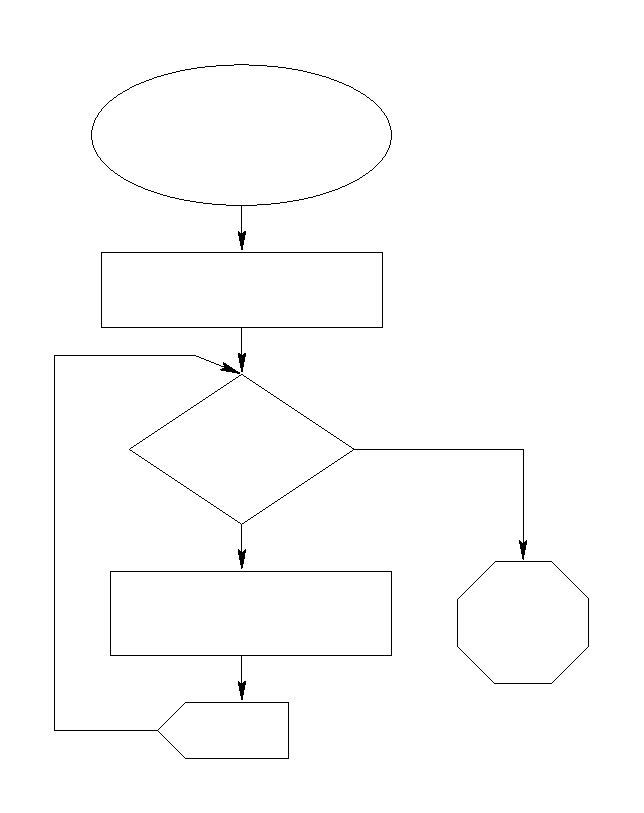
\includegraphics[scale=.5]{div_alg_flowchart.eps}} 
\caption{The division algorithm in flowchart form.}
\label{fig:div_alg}
\end{figure}

Note that in a flowchart the action of a ``Goto'' statement is clear
because an arrow points to the location where program flow is being
redirected.  In pseudocode a ``Label'' statement is required which
indicates a spot where flow can be redirected via subsequent ``Goto''
statements.  Because of the potential for confusion in complicated
algorithms that involve multitudes of Goto statements and their
corresponding Labels, this sort of redirection is now deprecated in
virtually all popular programming environments.

Before we move on to describe the Euclidean algorithm it might be
useful to describe more explicitly what exactly it's {\em for}.  
Given a pair of integers, $a$ and $b$, there are two quantities that 
it is important to be able to compute, the \index{least common multiple}
\emph{least common multiple}
or lcm, and the \index{greatest common divisor} 
\emph{greatest common divisor} or gcd.  The lcm also
goes by the name {\em lowest common denominator} because it is the
smallest denominator that could be used as a common denominator in the
process of adding two fractions that had $a$ and $b$ in their
denominators.  The gcd and the lcm are related by the formula 
\[ \lcm{a}{b} = \frac{ab}{\gcd{a}{b}}, \]
so they are essentially equivalent as far as representing a
computational challenge.

The \index{Euclidean algorithm} Euclidean algorithm depends 
on a rather extraordinary property of
the gcd.  Suppose that we are trying to compute $\gcd{a}{b}$ and that
$a$ is the larger of the two numbers.  We first feed $a$ and $b$ into
the division algorithm to find $q$ and $r$ such that $a = qb +r $.  It
turns out that $b$ and $r$ have the {\em same} gcd as did $a$ and
$b$.  In other words, $\gcd{a}{b} = \gcd{b}{r}$, furthermore these
numbers are smaller than the ones we started with!  This is nice
because it means we're now dealing with an easier version of the same
problem.  In designing an algorithm it is important to formulate a
clear {\em ending criterion}, a condition that tells you you're done.
In the case of the Euclidean algorithm, we know we're done when the
remainder $r$ comes out $0$.  

So, here, without further ado is the Euclidean algorithm in
pseudocode.  A flowchart version is given in Figure~\ref{fig:Euc_alg}.
\medskip

\begin{center}
\begin{minipage}[b]{.7\textwidth}
\tt Algorithm: Euclidean\\
Inputs: integers $a$ and $b$.\\
Local variables: $q$ and $r$.\\
\\
Label 1.\\
Let $(q,r)  = \mbox{Division}(a,b)$. \\
If $r = 0$ then\\
\rule{15pt}{0pt} Return $b$.\\
End If\\
Let $a = b$.\\
Let $b = r$.\\
Goto 1. \\
\end{minipage}
\end{center}

\begin{figure}[!hbt] 
\begin{center}
\begin{picture}(0,0)%
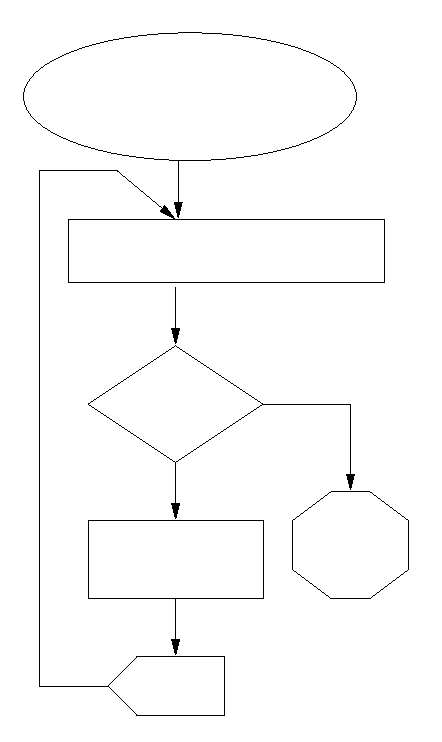
\includegraphics{figures/Euc_alg_flowchart.pdf}%
\end{picture}%
\setlength{\unitlength}{3947sp}%
%
\begingroup\makeatletter\ifx\SetFigFont\undefined%
\gdef\SetFigFont#1#2#3#4#5{%
  \reset@font\fontsize{#1}{#2pt}%
  \fontfamily{#3}\fontseries{#4}\fontshape{#5}%
  \selectfont}%
\fi\endgroup%
\begin{picture}(3527,5927)(0,-5087)
\put(937,-3767){\makebox(0,0)[lb]{\smash{{\SetFigFont{12}{14.4}{\familydefault}{\mddefault}{\updefault}{\color[rgb]{0,0,0}Let $b = r$.}%
}}}}
\put(2571,-3474){\makebox(0,0)[lb]{\smash{{\SetFigFont{12}{14.4}{\familydefault}{\mddefault}{\updefault}{\color[rgb]{0,0,0}Return:}%
}}}}
\put(2648,-3689){\makebox(0,0)[lb]{\smash{{\SetFigFont{12}{14.4}{\familydefault}{\mddefault}{\updefault}{\color[rgb]{0,0,0} $b$}%
}}}}
\put(937,-3552){\makebox(0,0)[lb]{\smash{{\SetFigFont{12}{14.4}{\familydefault}{\mddefault}{\updefault}{\color[rgb]{0,0,0}Let $a = b$.}%
}}}}
\put(1482,-3026){\makebox(0,0)[lb]{\smash{{\SetFigFont{12}{14.4}{\familydefault}{\mddefault}{\updefault}{\color[rgb]{0,0,0}No}%
}}}}
\put(2162,-2346){\makebox(0,0)[lb]{\smash{{\SetFigFont{12}{14.4}{\familydefault}{\mddefault}{\updefault}{\color[rgb]{0,0,0}Yes}%
}}}}
\put(1093,-2463){\makebox(0,0)[lb]{\smash{{\SetFigFont{12}{14.4}{\familydefault}{\mddefault}{\updefault}{\color[rgb]{0,0,0}Is $r = 0$?}%
}}}}
\put(626,-1219){\makebox(0,0)[lb]{\smash{{\SetFigFont{12}{14.4}{\familydefault}{\mddefault}{\updefault}{\color[rgb]{0,0,0}Let $(q,r)$ = Division($a,b$).}%
}}}}
\put(1171,-4718){\makebox(0,0)[lb]{\smash{{\SetFigFont{12}{14.4}{\familydefault}{\mddefault}{\updefault}{\color[rgb]{0,0,0}Goto}%
}}}}
\put(601,-136){\makebox(0,0)[lb]{\smash{{\SetFigFont{12}{14.4}{\familydefault}{\mddefault}{\updefault}{\color[rgb]{0,0,0}Local: integers $q$ \& $r$}%
}}}}
\put(601, 89){\makebox(0,0)[lb]{\smash{{\SetFigFont{12}{14.4}{\familydefault}{\mddefault}{\updefault}{\color[rgb]{0,0,0}Input: integers $a$ \& $b$}%
}}}}
\end{picture}%

\end{center}

%\centerline{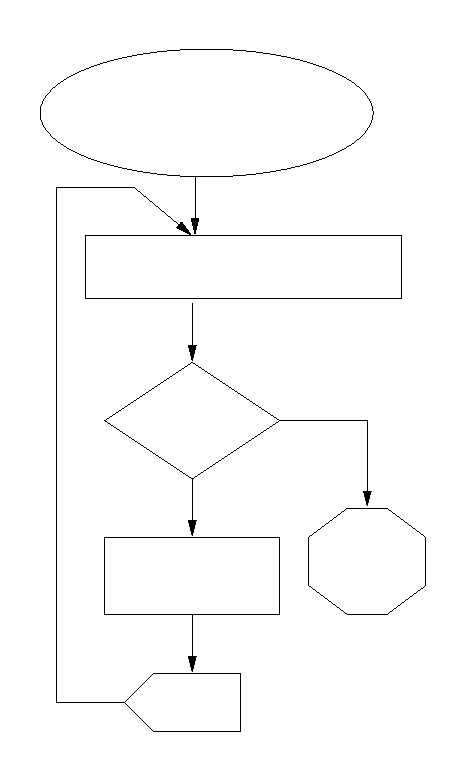
\includegraphics[scale=.5]{Euc_alg_flowchart.eps}} 
\caption{The Euclidean algorithm in flowchart form.}
\label{fig:Euc_alg}
\end{figure}

\clearpage 

It should be noted that for small numbers one can find the gcd and lcm
quite easily by considering their factorizations into primes.  For the
moment consider numbers that factor into primes but not into prime
powers (that is, their factorizations don't involve exponents).  The
gcd is the product of the primes that are in common between these
factorizations (if there are no primes in common it is 1).  The lcm is
the product of all the distinct primes 
that appear in the factorizations.  As an example, consider 30 and 42.
The factorizations are $30 = 2\cdot 3\cdot 5$ and $42 = 2\cdot 3 \cdot
7$.  The primes that are common to both factorizations are $2$ and
$3$, thus $\gcd{30}{42} = 2\cdot 3 = 6$.  The set of all the primes 
that appear in either factorization is $\{2, 3, 5, 7 \}$ so
$\lcm{30}{42} = 2\cdot 3\cdot 5\cdot 7 = 210$.

The technique just described is of little value for numbers having more
than about 50 decimal digits because it rests {\em a priori} on the
ability to find the prime factorizations of the numbers involved.
Factoring numbers is easy enough if they're reasonably small,
especially if some of their prime factors are small, but in general
the problem is considered so difficult that many cryptographic schemes
are based on it.
 
\newpage
  
\noindent{\large\bf Exercises --- \thesection\ }

\begin{enumerate}

\item Trace through the division algorithm with inputs $n=27$ and
  $d=5$, each time an assignment statement is encountered write it
  out.  How many assignments are involved in this particular
  computation?
\hint{r=27 \newline
q=0  \newline
r=27-5=22  \newline
q=0+1=1  \newline
r=22-5=17  \newline
q=1+1=2  \newline
r=17-5=12  \newline
q=2+1=3  \newline
r=12-5=7  \newline
q=3+1=4  \newline
r=7-5=2  \newline
q=4+1=5  \newline
return r is 2 and q is 5.
}

\wbvfill

\item Find the gcd's and lcm's of the following pairs of numbers.
\medskip

\centerline{
\begin{tabular}{|c|c|c|c|} \hline
\rule[-3pt]{0pt}{18pt} $a$ & $b$ & $\gcd{a}{b}$ & $\lcm{a}{b}$ \\ \hline
\rule[-3pt]{0pt}{18pt} 110 & 273 & & \\ \hline
\rule[-3pt]{0pt}{18pt}105 & 42 & & \\ \hline
\rule[-3pt]{0pt}{18pt}168 & 189 & & \\ \hline
\end{tabular}
}

\hint{For such small numbers you can just find their prime factorizations and use that, although it might be useful to practice your understanding of the Euclidean algorithm by tracing through it to find the gcd's and then using the formula
\[ \lcm (a,b) = \frac{ab}{\gcd (a,b).} \]
}

\workbookpagebreak

\item Formulate a description of the gcd of two numbers in terms of
  their prime factorizations in the general case (when the
  factorizations may include powers of the primes involved).

\wbvfill

\hint{Suppose that one number's prime factorization contains $p^e$ and the other
contains $p^f$, where $e < f$. What power of $p$ will divide both, $p^e$ or $p^f$ ?}

\item Trace through the Euclidean algorithm with inputs $a=3731$ and
  $b=2730$, each time the assignment statement that calls the division
  algorithm is encountered write out the expression $a=qb+r$.   (With the
  actual values involved !) 

\wbvfill

\hint{The quotients you obtain should alternate between 1 and 2.}

\end{enumerate}


\newpage

\section{Rational and irrational numbers}
\label{sec:rat}

When we first discussed the rational numbers in Section~\ref{sec:basic}
we gave the following definition, which isn't quite right.

\[ \Rationals = \{ \frac{a}{b} \suchthat a \in \Integers \; \mbox{and} \;
b \in \Integers \; \mbox{and} \; b \neq 0 \} \]

We are now in a position to fix the problem.

So what was the problem after all?  Essentially this: there are
many expressions formed with one integer written above another (with an
intervening fraction bar) that represent the exact same rational
number.  For example $\frac{3}{6}$ and $\frac{14}{28}$ are distinct
things that appear in the set defined above, but we all know that they
both represent the rational number $\frac{1}{2}$.  To eliminate this
problem with our definition of the rationals we need to add an
additional condition that ensures that such duplicates don't arise. 
It turns out that what we want is for the numerators and denominators
of our fractions to have {\em no} factors in common.  Another way to
say this is that the $a$ and $b$ from the definition above should be
chosen so that $\gcd{a}{b} = 1$.  A pair of numbers whose gcd is 1 are
called \index{relative primality} \emph{relatively prime}.

We're ready, at last, to give a good, precise  definition of the set
of rational numbers.   (Although it should be noted that we're not
quite done fiddling around; an even better definition will be given in
Section~\ref{sec:eq_rel}.)  

\[ \Rationals = \{ \frac{a}{b} \suchthat a,b \in \Integers \; \mbox{and} \;
b \neq 0 \; \mbox{and} \; \gcd{a}{b}=1 \}. \]

As we have in the past, let's parse this with an English translation in parallel.

\vspace{.2in}

\begin{tabular}{c|c|c}
\rule[-10pt]{0pt}{22pt} $\Rationals$ & $=$ & $\{$  \\ \hline
\rule[-6pt]{0pt}{22pt} The rational numbers & are defined to be & the set of all\\
\end{tabular}

\vspace{.2in}

\begin{tabular}{c|c|c}
\rule[-10pt]{0pt}{22pt} $\displaystyle \frac{a}{b}$ & $\suchthat$ & $a,b \in \Integers$ \\ \hline
\rule[-6pt]{0pt}{22pt} fractions of the form $a$ over $b$ & such that
& $a$ and $b$ are integers \\
\end{tabular}

\vspace{.2in}

\begin{tabular}{c|c|c|c|c}
\rule[-10pt]{0pt}{22pt} and & $b \neq 0$ & and & $\gcd{a}{b}=1$ & $\}$
\\ \hline
\rule[-6pt]{0pt}{22pt}  and & $b$ is non-zero & and & $a$ and $b$ are relatively prime. &  \\
\end{tabular}

\vspace{.2in}

Finally, we are ready to face a fundamental problem that was
glossed-over in Section~\ref{sec:basic}.  We defined two sets
back then, $\Rationals$ and $\Reals$, the hidden assumption that one
makes in asserting that there are two of something is that the two
things are distinct.  Is this really the case?  The reals have been
defined (unrigorously) as numbers that measure the magnitudes of
physical quantities, so another way to state the question is this:
Are there physical quantities (for example lengths) that are {\em not}
rational numbers?  

The answer is that {\em yes} there are numbers that measure lengths
which are not rational numbers.  With our new and improved definition
of what is meant by a rational number we are ready to {\em prove} that 
there is at least one length that can't be expressed as a fraction.
Using the Pythagorean theorem it's easy to see that the length of the
diagonal of a unit square is $\sqrt{\,2}$.  The proof that $\sqrt{\,2}$ is
not rational is usually attributed to the followers of Pythagoras (but
probably not to Pythagoras himself).  In any case it is a result of
great antiquity.  The proof is of a type known as 
\index{reductio ad absurdam} \emph{reductio ad absurdum}
\footnote{Reduction to an absurdity -- better known these %
days as proof by contradiction. }.  We show that a given assumption
leads logically to an absurdity, a statement that {\em can't} be true,
then we know that the original assumption must itself be false.  This 
method of proof is a bit slippery; one has to first assume the 
\emph{exact opposite} of what one hopes to prove and then argue (on
purpose) towards a ridiculous conclusion.

\begin{thm} The number $\sqrt{\,2}$ is not in the set $\Rationals$ of
rational numbers.
\end{thm}

Before we can actually give the proof we should prove an intermediary 
result -- but we won't, we'll save this proof for the student to do 
later (heh, heh, heh\ldots).
These sorts of intermediate results, things that don't deserve to be
called theorems themselves, but that aren't entirely self-evident are
known as \index{lemmas} lemmas.  It is often the case that in an 
attempt at proving a statement we find ourselves in need of some small 
fact.  Perhaps it even seems to be true but it's not clear.  In such 
circumstances, good form dictates that we first state and prove the 
lemma then proceed on to our theorem and its proof.  So, here, without 
its proof is the lemma we'll need.

\begin{lem} If the square of an integer is even, then the original
integer is even.
\end{lem}

Given that thoroughness demands that we fill in this gap by actually
proving the lemma at a later date, we can now proceed with the proof
of our theorem.   

\begin{proof}
Suppose to the contrary that $\sqrt{2}$ {\em is} a rational number.
Then by the definition of the set of rational numbers, we know that
there are integers 
$a$ and $b$ having the following properties: 
$\displaystyle \sqrt{2} = \frac{a}{b}$ and $\gcd{a}{b} = 1$.  

Consider the expression $\displaystyle \sqrt{2} = \frac{a}{b}$.   
By squaring both sides of this we obtain

\[ 2 = \frac{a^2}{b^2}. \]

This last expression can be rearranged to give

\begin{equation*}
a^2 = 2 b^2
\end{equation*}

An immediate consequence of this last equation is that $a^2$ is an
even number.  Using the lemma above we now know that $a$ is an even
integer and hence that there is an integer $m$ such that $a=2m$.
Substituting this last expression into the previous equation gives

\begin{equation*}
(2m)^2 = 2 b^2,
\end{equation*}

thus,

\begin{equation*}
4m^2 = 2 b^2,
\end{equation*}

so

\begin{equation*}
2m^2 = b^2.
\end{equation*}

This tells us that $b^2$ is even, and hence (by the lemma), $b$ is even.

Finally, we have arrived at the desired absurdity because if $a$ and
$b$ are both even then $\gcd{a}{b} \geq 2$, but, on the other hand,
one of our initial assumptions is that $\gcd{a}{b} = 1$. 

\end{proof}

\newpage

\noindent{\large\bf Exercises --- \thesection\ }

\begin{enumerate}

\item \index{Rational approximation} Rational Approximation is 
a field of mathematics that has received much study.  The main idea 
is to find rational numbers that are very good approximations to
given irrationals.  For example, $22/7$ is a well-known rational 
approximation to $\pi$.  Find good rational approximations to 
$\sqrt{2}, \sqrt{3}, \sqrt{5}$ and $e$.

\vfill

\wbvfill

\hint{One approach is to truncate a decimal approximation and then rationalize. E.g. $\sqrt{2}$ is approximately 1.4142, so 14142/10000 isn't a bad approximator (although naturally 7071/5000 is better since it involves smaller numbers).}

\vfill

\item The theory of base-$n$ notation that we looked at in 
\ifthenelse{\boolean{InTextBook}}{sub-section~\ref{base-n}}{the sub-section on base-$n$} can be extended to deal with real and 
rational numbers by introducing a decimal point (which should 
probably be re-named in accordance with the base) and adding 
digits to the right of it.  For instance $1.1011$ is binary notation
for $1 \cdot 2^0 + 1 \cdot 2^{-1} + 0 \cdot 2^{-2} + 
1\cdot 2^{-3} + 1\cdot 2^{-4}$ or $\displaystyle 1 + \frac{1}{2} + 
\frac{1}{8} + \frac{1}{16} = 1 \frac{11}{16}$.

Consider the binary number $.1010010001000010000010000001\ldots$, 
is this number rational or irrational?  Why?

\vfill

\hint{Does the rule about rational numbers having terminating or repeating decimal representations carry over to other bases?

\vfill

}

\workbookpagebreak
\hintspagebreak

\item If a number $x$ is even, it's easy to show that its square $x^2$
is even.  The lemma that went unproved in this section asks us to
start with a square ($x^2$) that is even and deduce that the UN-squared
number ($x$) is even.  Perform some numerical experimentation to
check whether this assertion is reasonable.  Can you give an argument
that would prove it?

\vfill

\hint{What if the lemma wasn't true? Can you work out what it would mean if we had a number x such that x2 was even but x itself was odd?}

\vfill

\item The proof that $\sqrt{2}$ is irrational can be generalized 
to show that $\sqrt{p}$ is irrational for every prime number $p$.
What statement would be equivalent to the lemma about the parity
of $x$ and $x^2$ in such a generalization?

\vfill

\hint{Hint: Saying ``x is even'' is the same thing as saying ``x is evenly divisible by 2.''  Replace the $2$ by $p$ and you're halfway there\ldots}

\vfill

\item Write a proof that $\sqrt{3}$ is irrational.

\vfill

\hint{You can mostly just copy the argument for $\sqrt{2}$.}

\vfill


\end{enumerate}

\newpage

\section{Relations}
\label{sec:rel_intro}

One of the principle ways in which mathematical writing
differs from ordinary writing is in its incredible brevity.  For
instance, a Ph.D. thesis for someone in the humanities would be very 
suspicious if its length were less than 300 pages, whereas it would
be quite acceptable for a math doctoral student to submit a thesis
amounting to less than 100 pages.  Indeed, the usual criteria for
a doctoral thesis (or indeed any scholarly work in mathematics) is
that it be ``new, true and interesting.''  If one can prove a truly 
interesting, novel result in a single page -- they'll probably hand over 
the sheepskin.

How is this great brevity achieved?  By inserting single symbols in place
of a whole paragraph's worth of words!  One class of symbols in particular
has immense power -- so-called \index{relations} relational symbols.  
When you place a relational
symbol between two expressions, you create a sentence that says the
relation \emph{holds}.  The period at the end of the last sentence should
probably be pronounced!  ``The relation holds, period!''  In other words
when you write down a mathematical sentence involving a relation, you 
are asserting the relation is True (the capital T is intentional).
This is why it's okay to write ``$2 < 3$'' but it's \emph{not} okay to
write ``$3 < 2$.''  The symbol $<$ is a relation symbol and you are
only supposed to put it between two things when they actually bear this
relation to one another.

The situation becomes slightly more complicated when we have 
variables in relational expressions, but before we proceed to
consider that complication let's make a list of the relations
we've seen to date:

\[ =, <, >, \leq, \geq,\; \divides \; , \; \mbox{and} \; \equiv \pmod{m}. \] 

Each of these, when placed between numbers, produces a statement that
is either true or false.  Ordinarily we wouldn't write down the 
false ones, instead we should express that we know the relation
\emph{doesn't} hold by negating the relation symbol (often by
drawing a slash through it, but some of the symbols above are
negations of others).

So what about expressions involving variables and these relation symbols?
For example what does $x < y$ really mean?  Okay, I know that you know 
what $x < y$ means but, philosophically, a relation symbol involving variables
is doing something that you may have only been vaguely aware of in the 
past -- it is introducing a \emph{supposition}.  Watch out for relation
symbols involving variables!  Whenever you encounter them it means the 
rules of the game are being subtly altered -- up until the point where 
you see $x < y$, $x$ and $y$ are just two random numbers, but after that
point we must suppose that $x$ is the smaller of the two.

The relations we've discussed so far are \index{binary relation} 
\emph{binary} relations, that
is, they go in between \emph{two} numbers.  There are also higher order
relations.  For example, a famous \index{ternary relation} ternary 
relation (a relationship between
three things) is the notion of ``betweenness.''  If $A$, $B$ and $C$ are
three points which all lie on a single line, we write $A\star B \star C$
if $B$ falls somewhere on the line segment $\overline{AC}$.  So the
symbol $A\star B \star C$ is shorthand for the sentence ``Point $B$ lies
somewhere in between points $A$ and $C$ on the line determined by them.''

There is a slightly silly tendency these days to define functions as being
a special class of relations.  (This is slightly silly not because it's wrong
-- indeed, functions are a special type of relation -- but because it's the 
least intuitive approach possible, and it is usually foisted-off on middle or
high school students.)  When this approach is taken, we first define
a relation to be \emph{any} set of ordered pairs and then state a 
restriction on the ordered pairs that may be in a relation if it 
is to be a function.  Clearly what these Algebra textbook authors 
are talking about are \emph{binary} relations, a ternary relation 
would actually be a set of ordered triples, and higher order relations
might involve ordered 4-tuples or 5-tuples, etc.  A couple of small examples 
should help to clear up this connection between a relation symbol and 
some set of tuples.

Consider the numbers from 1 to 5 and the less-than relation, $<$.  
As a set of ordered pairs, this relation is the set 

\[ \{(1,2), (1,3), (1,4), (1,5), (2,3), (2,4), (2,5), (3,4), (3,5), (4,5) \}. \]

The pairs that are \emph{in} the relation are those such that the first is smaller than the second.

An example involving the ternary relation ``betweenness'' can be had 
from the following diagram.
\medskip

\begin{picture}(0,0)%
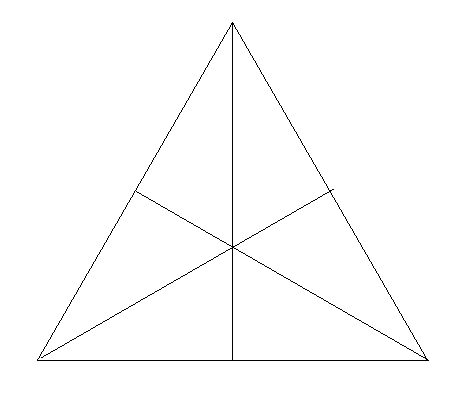
\includegraphics{figures/betweenness_example.pdf}%
\end{picture}%
\setlength{\unitlength}{3947sp}%
%
\begingroup\makeatletter\ifx\SetFigFont\undefined%
\gdef\SetFigFont#1#2#3#4#5{%
  \reset@font\fontsize{#1}{#2pt}%
  \fontfamily{#3}\fontseries{#4}\fontshape{#5}%
  \selectfont}%
\fi\endgroup%
\begin{picture}(3585,3268)(2941,-2861)
\put(4906,284){\makebox(0,0)[lb]{\smash{{\SetFigFont{12}{14.4}{\familydefault}{\mddefault}{\updefault}{\color[rgb]{0,0,0}$A$}%
}}}}
\put(6511,-2611){\makebox(0,0)[lb]{\smash{{\SetFigFont{12}{14.4}{\familydefault}{\mddefault}{\updefault}{\color[rgb]{0,0,0}$C$}%
}}}}
\put(4711,-2806){\makebox(0,0)[lb]{\smash{{\SetFigFont{12}{14.4}{\familydefault}{\mddefault}{\updefault}{\color[rgb]{0,0,0}$D$}%
}}}}
\put(2956,-2731){\makebox(0,0)[lb]{\smash{{\SetFigFont{12}{14.4}{\familydefault}{\mddefault}{\updefault}{\color[rgb]{0,0,0}$E$}%
}}}}
\put(3631,-1126){\makebox(0,0)[lb]{\smash{{\SetFigFont{12}{14.4}{\familydefault}{\mddefault}{\updefault}{\color[rgb]{0,0,0}$F$}%
}}}}
\put(4921,-1621){\makebox(0,0)[lb]{\smash{{\SetFigFont{12}{14.4}{\familydefault}{\mddefault}{\updefault}{\color[rgb]{0,0,0}$G$}%
}}}}
\put(5701,-1096){\makebox(0,0)[lb]{\smash{{\SetFigFont{12}{14.4}{\familydefault}{\mddefault}{\updefault}{\color[rgb]{0,0,0}$B$}%
}}}}
\end{picture}%

\medskip

The betweenness relation on the points in this diagram consists of the 
following triples.

\begin{gather*} \{ (A,B,C), (A,G,D), (A,F,E), (B,G,E), (C,B,A), (C,G,F), (C,D,E), \\
(D,G,A), (E,D,C), (E,G,B), (E,F,A), (F,G,C) \}. 
\end{gather*}

\begin{exer}
When thinking of a function as a special type of relation, the pairs are of
the form $(x, f(x))$.  That is, they consist of an input and the corresponding
output.  What is the restriction that must be placed on the pairs in a 
relation if it is to be a function?  (Hint: think about the so-called 
vertical line test.)
\end{exer}

\newpage

\noindent{\large\bf Exercises --- \thesection\ }

\begin{enumerate}

\item Consider the numbers from 1 to 10.  Give the set of pairs of these numbers that 
corresponds to the divisibility relation.

\vfill

\hint{A pair is ``in'' the relation when the first number gazinta the second number.  $1$ gazinta anything, $2$ gazinta the even numbers, $3$ gazinta $3$, $6$ and $9$, etc. (Also a number always gazinta itself.)}

\vfill

\item The \index{domain}\emph{domain} of a function (or binary relation) 
is the set of numbers appearing in the first coordinate.  The \index{range} 
\emph{range} of a function (or binary relation) is the set of numbers 
appearing in the second coordinate.  

Consider the set $\{0,1,2,3,4,5,6\}$ and the function $f(x) = x^2 \pmod{7}$.
Express this function as a relation by explicitly writing out the set of
ordered pairs it contains.  What is the range of this function?
 
 \vfill
 
\hint{
\[ f \; = \; \{(0,0), (1,1), (2,4), (3,2), (4,2), (5,4), (6,1)\} \]
\[ \Rng{f} \;= \; \{0,1,2,4\} \]

}

\vfill

\workbookpagebreak
\hintspagebreak

\item What relation on the numbers from 1 to 10 does the following set of ordered pairs
represent?

\begin{gather*}
\{ (1,1), (1,2), (1,3), (1,4), (1,5), (1,6), (1,7), (1,8), (1,9), (1,10), \\
(2,2), (2,3), (2,4), (2,5), (2,6), (2,7), (2,8), (2,9), (2,10), \\
(3,3), (3,4), (3,5), (3,6), (3,7), (3,8), (3,9), (3,10), \\
(4,4), (4,5), (4,6), (4,7), (4,8), (4,9), (4,10), \\
(5,5), (5,6), (5,7), (5,8), (5,9), (5,10), \\
(6,6), (6,7), (6,8), (6,9), (6,10), \\
(7,7), (7,8), (7,9), (7,10), \\
(8,8), (8,9), (8,10), \\
(9,9), (9,10), \\
(10,10) \} 
\end{gather*}

\vfill

\hint{ Less-than-or-equal-to }

\vfill

\hintspagebreak
\workbookpagebreak

\item Draw a five-pointed star, label all 10 points. There are 40 triples of these 
labels that satisfy the betweenness relation.  List them.

\vfill

\hint{
Yeah, hmmm. Forty is kind of a lot...
Let's look at the points (E,F,G and B) on the horizontal line in the diagram below. The triples involving these four points are: (E,F,G), (G,F,E), (E,F,B), (B,F,E), (E,G,B), (B,G,E), (F,G,B), (B,G,F).

\vfill

\centerline{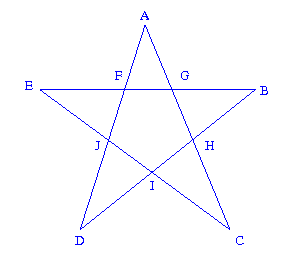
\includegraphics{figures/star}}

\vfill

}

\workbookpagebreak

\item Sketch a graph of the relation 
\[
\{ (x,y) \suchthat x,y \in \Reals \; \mbox{and} \; y > x^2 \}.
\]

\hint{Is this the region above or below the curve $y=x^2$?}

\wbvfill

\item A function $f(x)$ is said to be \index{invertible function} 
\emph{invertible} if there is another function $g(x)$ such that 
$g(f(x)) = x$ for all values of $x$.  (Usually, the inverse function,
$g(x)$ would be denoted $f^{-1}(x)$.)   Suppose a function is presented 
to you as a relation -- that is, you are just given a set of pairs.  
How can you distinguish whether the function represented by this list 
of input/output pairs is invertible?  How can you produce the inverse 
(as a set of ordered pairs)?
 
\hint{If $f$ sends $x$ to $y$, then we want $f^{-1}$ to send $y$ back to $x$.  So the inverse just has the pairs in $f$ reversed.  When is the inverse going to fail to be a function?}

\wbvfill

\workbookpagebreak

\item There is a relation known as ``has color'' which goes from the
set 
\[ F = \{orange, cherry, pumpkin, banana\} \]
to the set 
\[ C = \{orange, red, green, yellow\}. \]

\noindent  What pairs are in ``has color''?
   
\hint{Depending on your personal experience level with fruit there may be different answers.  Certainly
(orange, orange) will be one of the pairs, but (orange, green) happens too!}

\wbvfill

\end{enumerate}



%\newpage
%\renewcommand{\bibname}{References for chapter 1}
%\bibliographystyle{plain}
%\bibliography{main}

%% Emacs customization
%% 
%% Local Variables: ***
%% TeX-master: "GIAM.tex" ***
%% comment-column:0 ***
%% comment-start: "%% "  ***
%% comment-end:"***" ***
%% End: ***



\chapter{Logic and quantifiers}
\label{ch:logic}

{\em If at first you don't succeed, try again. Then quit. There's no use being a damn fool about it. --W. C. Fields}

\section{Predicates and Logical Connectives}
\label{sec:pred}

In every branch of Mathematics there are special, \index{atomic concepts}
atomic, notions that
defy precise definition.  In Geometry, for example, the atomic notions
are points, lines and their incidence.  Euclid defines a point as
``that which has no part'' -- people can argue (and have argued) incessantly
over what exactly is meant by this.  Is it essentially saying that anything 
without volume, area or length of some sort is a point?  In modern times
it has been recognized that any formal system of argumentation has to
have such elemental, undefined, concepts -- and that Euclid's apparent
lapse in precision comes from an attempt to hide this basic fact.
The notion of ``point'' can't really {\em be} defined.  All we can do
is point (no joke intended) at a variety of points and hope that our
audience will absorb the same concept of point that we hold via the 
process of \index{induction}induction\footnote{inference of a %
generalized conclusion from particular instances -- compare DEDUCTION}.

The atomic concepts in Set Theory are ``set'', ``element'' and ``membership''.
The atomic concepts in Logic are ``true'', ``false'', \index{sentence} 
``sentence'' and \index{statement} ``statement''.  

Regarding {\em true} and {\em false}, we hope there is no uncertainty
as to their meanings.  {\em Sentence} also has a well-understood
meaning that most will agree on -- a syntactically correct ordered collection
of words such as ``Johnny was a football player.'' or ``Red is a color.''
or ``This is a sentence which does not refer to itself.''  A {\em statement}
is a sentence which is either true or false.  
In other words, a statement
is a sentence whose truth value is {\em definite}, in more other words,
it is always possible to decide -- one way or the other -- whether
a statement is true or false.\footnote{Although, as a practical matter
it may be almost impossibly difficult to do so!  For instance it is 
certainly either true or false that I ate eggs for breakfast on my 21st
birthday -- but I don't remember, and short of building a time machine,
I don't know how you could find out.}   The first example
of a sentence given above (``Johnny was a football player'') is not a 
statement -- the problem is that it is ambiguous unless we know who
Johnny is.  If it had said ``Johnny Unitas was a football player.'' then
it would have been a statement.  If it had said ``Johnny Appleseed was a 
football player.'' it would also have been a statement, just not a true one.

Ambiguity is only one reason that a sentence may not be a statement.  As 
we consider more complex sentences, it may be the case that the truth
value of a given sentence simply cannot be decided.  One of the most
celebrated mathematical results of the 20th century is 
\index{G\"{o}del, Kurt}Kurt G\"{o}del's
\index{Incompleteness Theorem}``Incompleteness Theorem.''  
An important aspect of this theory is 
the proof that in any axiomatic system of mathematical thought
there must be undecidable sentences -- statements which can neither be proved
nor disproved from the axioms\footnote{There are trivial systems that %
are complete, but if a system is sufficiently complicated that it contains %
``interesting'' statements it can't be complete.}.  
Simple sentences (e.g. those of the form 
subject-verb-object) have little chance of being undecidable for this
reason, so we will next look at ways of building more complex sentences
from simple components. 

Let's start with an example.  Suppose I come up to you in some windowless
room and make the statement: ``The sun is shining but it's raining!''  
You decide to investigate my claim and determine its veracity.  Upon
reaching a room that has a view of the exterior there are four possible
combinations of sunniness and/or precipitation that you may find.  That is,
the atomic predicates ``The sun is shining'' and ``It is raining'' can each 
be true or false independently of one another.  In the following table 
we introduce a convention used throughout the remainder of this book -- 
that true is indicated with a capital letter T and false is indicated 
with the Greek letter $\phi$ (which is basically a Greek F, and is a lot harder
to mistake for a T than an F is.)

\begin{center}
\begin{tabular}{c|c}
The sun is shining \; & \; It is raining \\ \hline
T & T \\
T & $\phi$ \\
 $\phi$ & T \\
 $\phi$ &  $\phi$ \\
\end{tabular}
\end{center}

Each row of the above table represents a possible state of the outside 
world.  Suppose you observe the conditions given in the last row, namely
that it is neither sunny, nor is it raining -- you would certainly conclude
that I am not to be trusted.  I.e. my statement, the compounding of 
``The sun is shining'' and ``It is raining'' (with the word ``but'' in between
as a connector) is false.  If you think about it a bit, you'll agree that
this so-called \index{compound sentence}{\em compound sentence} is true 
only in the case that both
of its component pieces are true.  This underscores an amusing linguistic
point: ``but'' and ``and'' have exactly the same meaning!  More precisely,
they {\em denote} the same thing, they have subtly different connotations
however -- ``but'' indicates that both of the statements it connects
are true and that the speaker is surprised by this state of affairs.

In Mathematics we distinguish two main connectives for hooking-up simple
sentences into compound ones.  The \index{conjunction}{\em conjunction} 
of two sentences is
the compound sentence made by sticking the word ``and'' between them.
The \index{disjunction}{\em disjunction} of two sentences is 
formed by placing an ``or'' 
between them.  Conjunctions are true only when both components are true.
Disjunctions are false only when both components are false.


As usual, mathematicians have developed an incredibly terse, compact
notation for these ideas.\footnote{One begins to suspect that %
mathematicians form an unusually lazy sub-species of humanity.}  
First, we represent an
entire sentence by a single letter -- traditionally, a capital letter.  
This is called a \index{predicate variable}{\em predicate variable}.
For example, following the example above, we could denote the sentence
``The sun is shining'' by the letter $S$.   Similarly, we could make the
assignment $R =$ ``It is raining.''   The conjunction and disjunction 
of these sentences can then be represented using the symbols $S \land R$
and $S \lor R$, respectively.  As a mnemonic, note that the connective
in $S \land R$ looks very much like the capital letter A (as in And).

To display, very succinctly, the effect of these two connectives we can
use so-called \index{truth table}truth tables. In a truth table we list 
all possible truth 
values of the predicate variables and then enumerate the truth values 
of some compound sentence.  For the conjunction and disjunction
connectors we have (respectively):

\begin{center}
\begin{tabular}{c|c||c}
\; $A$ \; & \; $B$ \; & \; $A \land B$ \; \\ \hline
T & T & T \\
T & $\phi$ & $\phi$\\
 $\phi$ & T & $\phi$\\
 $\phi$ &  $\phi$ & $\phi$\\
\end{tabular}
\hspace{.25in}and\hspace{.25in}
\begin{tabular}{c|c||c}
\; $A$ \; & \; $B$ \; & \; $A \lor B$ \; \\ \hline
T & T & T \\
T & $\phi$ & T\\
 $\phi$ & T & T\\
 $\phi$ &  $\phi$ & $\phi$\\
\end{tabular}.
\end{center}

In addition to these connectors we need a modifier (called 
\index{negation}{\em negation}) 
that acts on individual sentences.  The negation of a sentence $A$ is 
denoted by ${\lnot}A$, and its truth value is exactly the opposite of
$A$'s truth value.  The negation of a sentence is also known as the
\emph{denial} of a sentence. 
A truth table for the negation operator is somewhat 
trivial but we include it here for completeness.

\begin{center}
\begin{tabular}{c||c}
\; $A$ \; &  \; ${\lnot}A$ \; \\ \hline
 T & $\phi$ \\
 $\phi$ & T \\
\end{tabular}
\end{center}

These three simple tools (and, or \& not) are sufficient to 
create extraordinarily complex sentences out of basic components.
The way these pieces interrelate is a bit reminiscent of algebra,
in fact the study of these logical operators (or any
 operators that act like them) is called \index{Boole, George}
 {\em Boolean Algebra}\footnote{In honor of George Boole, whose 1854 %
 book {\em An investigation into the Laws of Thought} inaugurated the %
 subject.}.   There are distinct differences
between Boolean and ordinary algebra however.  In regular algebra we have
the binary connectors $+$ (plus) and $\cdot$ (times), and the unary 
negation operator $-$, these are certainly analogous to $\land$, $\lor$ \&
$\lnot$, but there are certain consequences of the fact that multiplication
is effectively repeated addition that simply don't hold for the Boolean
operators.  For example, there is a well-defined precedence between $\cdot$ and
$+$.   In parsing the expression $4 \cdot 5 + 3$ we all know that the 
multiplication is to be done first.  There is no such rule governing
order of operations between $\land$ and $\lor$, so an expression like
$A \land B \lor C$ is simply ambiguous -- it {\em must} have parentheses
inserted in order to show the order, either  $(A \land B) \lor C$ or 
$A \land (B \lor C)$.  Another distinction between ordinary and Boolean
algebra is exponentiation.  If there {\em were} exponents in Boolean algebra,
we'd need two different kinds -- one for repeated conjunction and another
for repeated disjunction. 

\begin{exer} 
Why is it that there is no such thing as exponentiation
in the algebra of Logic?
\end{exer}

While there are many differences between Boolean algebra and the
usual, garden-variety algebra, there are also many similarities.
For instance, the \index{associative law}associative, 
\index{commutative law}commutative and 
\index{distributive law}distributive laws
of Algebra all have versions that work in the Boolean case.

A very handy way of visualizing Boolean expressions is given by
digital logic circuit diagrams.  To discuss these diagrams we 
must make a brief digression into Electronics.  One of the most
basic components inside an electronic device is a \index{transistor}
transistor,
this is a component that acts like a switch for electricity,
but the switch itself is controlled by electricity.  In Figure~\ref{fig:trans}
we see the usual schematic representation of a transistor.  If voltage
is applied to the wire labeled z, the transistor becomes conductive,
and current may flow from x to y.  

\begin{figure}[!hbtp] 
\begin{center}
\begin{picture}(0,0)%
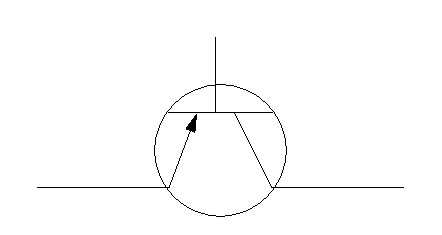
\includegraphics{./transistor.pdf}%
\end{picture}%
\setlength{\unitlength}{3947sp}%
%
\begingroup\makeatletter\ifx\SetFigFont\undefined%
\gdef\SetFigFont#1#2#3#4#5{%
  \reset@font\fontsize{#1}{#2pt}%
  \fontfamily{#3}\fontseries{#4}\fontshape{#5}%
  \selectfont}%
\fi\endgroup%
\begin{picture}(3527,1877)(1350,-2462)
\put(1501,-2161){\makebox(0,0)[lb]{\smash{{\SetFigFont{12}{14.4}{\familydefault}{\mddefault}{\updefault}{\color[rgb]{0,0,0}x}%
}}}}
\put(3076,-811){\makebox(0,0)[lb]{\smash{{\SetFigFont{12}{14.4}{\familydefault}{\mddefault}{\updefault}{\color[rgb]{0,0,0}z}%
}}}}
\put(4651,-2161){\makebox(0,0)[lb]{\smash{{\SetFigFont{12}{14.4}{\familydefault}{\mddefault}{\updefault}{\color[rgb]{0,0,0}y}%
}}}}
\end{picture}%

\end{center}
\caption{A schematic representation of a transistor.}
\label{fig:trans}
\end{figure}

Suppose that two transistors are connected as in Figure~\ref{fig:series}
(this is called a \index{series connection}{\em series} connection).  
In order for current to flow
from x to y we must have voltage applied to {\em both} the wires labeled
z and w.  In other words, this circuit effectively creates the {\bf and} 
operation --  assuming voltage is always applied to x, if z {\bf and} w
are energized then the output at y will be energized.

\begin{figure}[!hbtp] 
\begin{center}
\begin{picture}(0,0)%
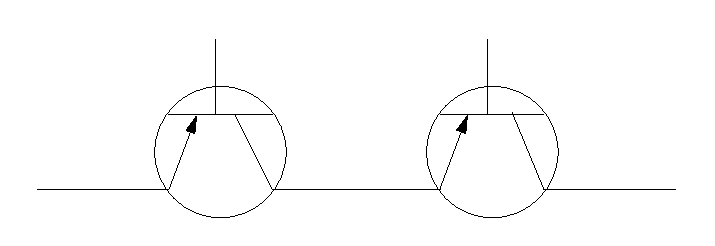
\includegraphics{figures/series.pdf}%
\end{picture}%
\setlength{\unitlength}{3947sp}%
%
\begingroup\makeatletter\ifx\SetFigFont\undefined%
\gdef\SetFigFont#1#2#3#4#5{%
  \reset@font\fontsize{#1}{#2pt}%
  \fontfamily{#3}\fontseries{#4}\fontshape{#5}%
  \selectfont}%
\fi\endgroup%
\begin{picture}(5702,1952)(1350,-2537)
\put(1501,-2161){\makebox(0,0)[lb]{\smash{{\SetFigFont{12}{14.4}{\familydefault}{\mddefault}{\updefault}{\color[rgb]{0,0,0}x}%
}}}}
\put(3076,-811){\makebox(0,0)[lb]{\smash{{\SetFigFont{12}{14.4}{\familydefault}{\mddefault}{\updefault}{\color[rgb]{0,0,0}z}%
}}}}
\put(5251,-811){\makebox(0,0)[lb]{\smash{{\SetFigFont{12}{14.4}{\familydefault}{\mddefault}{\updefault}{\color[rgb]{0,0,0}w}%
}}}}
\put(6826,-2161){\makebox(0,0)[lb]{\smash{{\SetFigFont{12}{14.4}{\familydefault}{\mddefault}{\updefault}{\color[rgb]{0,0,0}y}%
}}}}
\end{picture}%

\end{center}
\caption[Series connections implement \emph{and}.]{%
The connection of two transistors in series provides %
an implementation of the {\em and} operator.}
\label{fig:series}
\end{figure}

When two transistors are connected in \index{parallel connection}parallel (this is illustrated in
Figure~\ref{fig:par}) current can flow from x to y when either (or {\em both})
of the wires at z and w have voltage applied.  This brings up a point
which is confusing for some: in common speech the use of the word ``or'' often
has the sense known as \index{exclusive or}{\em exclusive or} (a.k.a. xor), when we say ``X or Y''
we mean ``Either X or Y, but not both.''  In Electronics and Mathematics,
{\em or} always has the non-exclusive (better known as 
\index{inclusive or}inclusive) sense.

\begin{figure}[!hbtp] 
\begin{center}
\begin{picture}(0,0)%
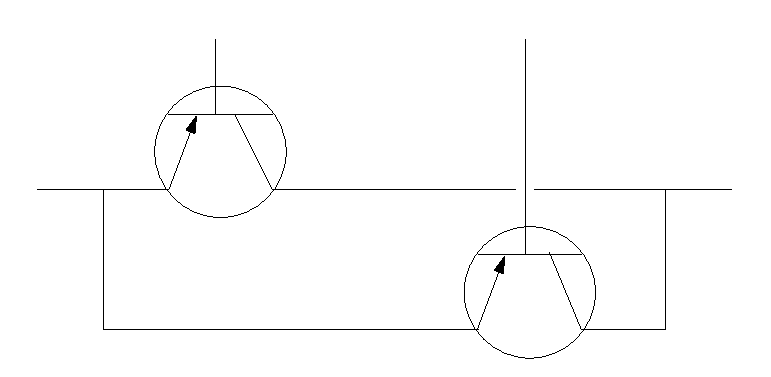
\includegraphics{./parallel.pdf}%
\end{picture}%
\setlength{\unitlength}{3947sp}%
%
\begingroup\makeatletter\ifx\SetFigFont\undefined%
\gdef\SetFigFont#1#2#3#4#5{%
  \reset@font\fontsize{#1}{#2pt}%
  \fontfamily{#3}\fontseries{#4}\fontshape{#5}%
  \selectfont}%
\fi\endgroup%
\begin{picture}(6152,3002)(1350,-3587)
\put(1501,-2161){\makebox(0,0)[lb]{\smash{{\SetFigFont{12}{14.4}{\familydefault}{\mddefault}{\updefault}{\color[rgb]{0,0,0}x}%
}}}}
\put(3076,-811){\makebox(0,0)[lb]{\smash{{\SetFigFont{12}{14.4}{\familydefault}{\mddefault}{\updefault}{\color[rgb]{0,0,0}z}%
}}}}
\put(5551,-811){\makebox(0,0)[lb]{\smash{{\SetFigFont{12}{14.4}{\familydefault}{\mddefault}{\updefault}{\color[rgb]{0,0,0}w}%
}}}}
\put(7276,-2161){\makebox(0,0)[lb]{\smash{{\SetFigFont{12}{14.4}{\familydefault}{\mddefault}{\updefault}{\color[rgb]{0,0,0}y}%
}}}}
\end{picture}%

\end{center}
\caption[Parallel connections implement \emph{or}.]{%
The connection of two transistors in parallel provides %
an implementation of the {\em or} operator.}
\label{fig:par}
\end{figure}

\newpage

As a sort of \index{logic gates}graphical shorthand, electronics engineers use the symbols
below to indicate \index{and gates}and-gates, \index{or gates}or-gates \& \index{not gates}not-gates (better known as negators).

\begin{center}
\begin{picture}(0,0)%
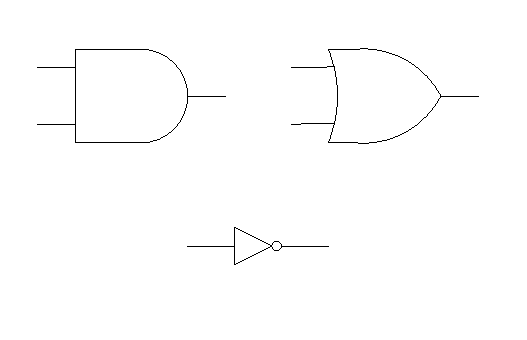
\includegraphics{figures/gates.pdf}%
\end{picture}%
\setlength{\unitlength}{3947sp}%
%
\begingroup\makeatletter\ifx\SetFigFont\undefined%
\gdef\SetFigFont#1#2#3#4#5{%
  \reset@font\fontsize{#1}{#2pt}%
  \fontfamily{#3}\fontseries{#4}\fontshape{#5}%
  \selectfont}%
\fi\endgroup%
\begin{picture}(4202,2702)(300,-2162)
\put(2026,-1861){\makebox(0,0)[lb]{\smash{{\SetFigFont{12}{14.4}{\familydefault}{\mddefault}{\updefault}{\color[rgb]{0,0,0}Not ($\lnot$)}%
}}}}
\put(2926,-961){\makebox(0,0)[lb]{\smash{{\SetFigFont{12}{14.4}{\familydefault}{\mddefault}{\updefault}{\color[rgb]{0,0,0}Or ($\lor$)}%
}}}}
\put(901,-961){\makebox(0,0)[lb]{\smash{{\SetFigFont{12}{14.4}{\familydefault}{\mddefault}{\updefault}{\color[rgb]{0,0,0}And ($\land$)}%
}}}}
\end{picture}%

\end{center}

An and-gate has two transistors inside it that are wired in series -- 
if both the inputs are energized the output will be too.  An
or-gate has two transistors in parallel inside it.  Not-gates 
involve magic -- when their input is not on, their output \emph{is}
and vice versa.

Using this graphical ``language'' one can make schematic 
representations of logical expressions.  Some find that 
tracing such diagrams makes understanding the structure 
of a Boolean expression easier.  For example, in Figure~\ref{fig:3ands}
we illustrate 2 of the possible ways that the conjunction
of four predicate variables can be parenthesized.  In fact, when
a multitude of predicates are joined by the same connective,
the way in which the expression is parenthesized is unimportant,
thus one often sees a further shorthand --- gates with more than
2 inputs.

\begin{figure}[!hbtp] 
\centerline{\begin{picture}(0,0)%
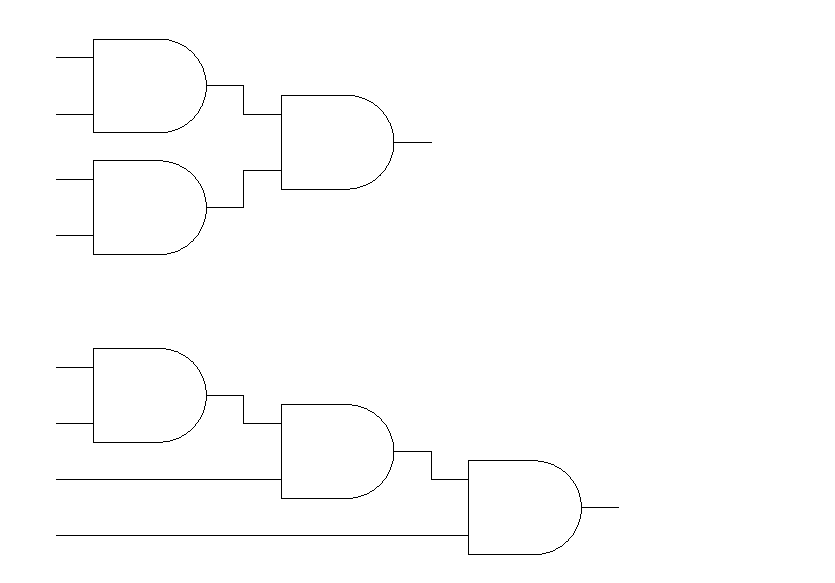
\includegraphics{figures/3_ands.pdf}%
\end{picture}%
\setlength{\unitlength}{3947sp}%
%
\begingroup\makeatletter\ifx\SetFigFont\undefined%
\gdef\SetFigFont#1#2#3#4#5{%
  \reset@font\fontsize{#1}{#2pt}%
  \fontfamily{#3}\fontseries{#4}\fontshape{#5}%
  \selectfont}%
\fi\endgroup%
\begin{picture}(6677,4652)(600,-4412)
\put(4126,-961){\makebox(0,0)[lb]{\smash{{\SetFigFont{12}{14.4}{\familydefault}{\mddefault}{\updefault}{\color[rgb]{0,0,0}$((A \land B) \land (C \land D))$}%
}}}}
\put(5626,-3886){\makebox(0,0)[lb]{\smash{{\SetFigFont{12}{14.4}{\familydefault}{\mddefault}{\updefault}{\color[rgb]{0,0,0}$(((A \land B) \land C) \land D)$}%
}}}}
\put(826,-286){\makebox(0,0)[lb]{\smash{{\SetFigFont{12}{14.4}{\familydefault}{\mddefault}{\updefault}{\color[rgb]{0,0,0}$A$}%
}}}}
\put(826,-736){\makebox(0,0)[lb]{\smash{{\SetFigFont{12}{14.4}{\familydefault}{\mddefault}{\updefault}{\color[rgb]{0,0,0}$B$}%
}}}}
\put(826,-1261){\makebox(0,0)[lb]{\smash{{\SetFigFont{12}{14.4}{\familydefault}{\mddefault}{\updefault}{\color[rgb]{0,0,0}$C$}%
}}}}
\put(826,-1711){\makebox(0,0)[lb]{\smash{{\SetFigFont{12}{14.4}{\familydefault}{\mddefault}{\updefault}{\color[rgb]{0,0,0}$D$}%
}}}}
\put(826,-2761){\makebox(0,0)[lb]{\smash{{\SetFigFont{12}{14.4}{\familydefault}{\mddefault}{\updefault}{\color[rgb]{0,0,0}$A$}%
}}}}
\put(826,-3211){\makebox(0,0)[lb]{\smash{{\SetFigFont{12}{14.4}{\familydefault}{\mddefault}{\updefault}{\color[rgb]{0,0,0}$B$}%
}}}}
\put(826,-3661){\makebox(0,0)[lb]{\smash{{\SetFigFont{12}{14.4}{\familydefault}{\mddefault}{\updefault}{\color[rgb]{0,0,0}$C$}%
}}}}
\put(826,-4111){\makebox(0,0)[lb]{\smash{{\SetFigFont{12}{14.4}{\familydefault}{\mddefault}{\updefault}{\color[rgb]{0,0,0}$D$}%
}}}}
\end{picture}%
}
\caption[Parenthesizations expressed as digital logic circuits.]{%
Two of the possible ways to parenthesize the conjunction %
of four statement variables -- expressed as digital logic circuits.}
\label{fig:3ands}
\end{figure}

A common task for an electronics designer is to come up with
a digital logic circuit having a prescribed input/output table.
Note that an input/output table for a logic circuit is entirely
analogous with a truth table for a compound sentence in Logic ---
except that we use 0's and 1's rather than T's and $\phi$'s.

Suppose that we wanted to design a circuit that would
have the following input/output table.

\begin{center}
\begin{tabular}{c|c|c|c}
$\; x \;$ & $\; y \;$ & $\; z \;$ & \rule{5pt}{0pt} out \rule{5pt}{0pt} \\ \hline
0 & 0 & 0 & 0 \\
0 & 0 & 1 & 0 \\
0 & 1 & 0 & 0 \\
0 & 1 & 1 & 1 \\ \hline
1 & 0 & 0 & 0 \\ 
1 & 0 & 1 & 0 \\ 
1 & 1 & 0 & 1 \\ 
1 & 1 & 1 & 1 \\
\end{tabular}
\end{center}

A systematic method for accomplishing such a design task involves
a notion called \index{disjunctive normal form}{\em disjunctive normal form}.  
A Boolean expression
is in disjunctive normal form if it consists of the disjunction of 
one or more statements, each of which consists entirely of conjunctions
of predicate variables and/or their negations.  In other words, the {\em or}
of a bunch of {\em ands}.  In terms of digital logic circuits, the {\em and}s 
we're talking about are called \index{recognizers}{\em recognizers}.  
For example,
the following 3-input and-gates recognize the input states in
the 4th, 7th and 8th rows of the i/o table above. (These are the rows 
where the output is supposed to be 1.)

\begin{center}
\begin{picture}(0,0)%
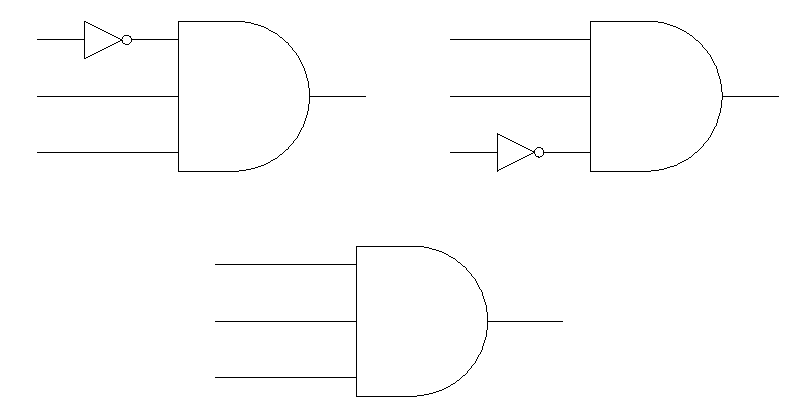
\includegraphics{./recognizers.pdf}%
\end{picture}%
\setlength{\unitlength}{3947sp}%
%
\begingroup\makeatletter\ifx\SetFigFont\undefined%
\gdef\SetFigFont#1#2#3#4#5{%
  \reset@font\fontsize{#1}{#2pt}%
  \fontfamily{#3}\fontseries{#4}\fontshape{#5}%
  \selectfont}%
\fi\endgroup%
\begin{picture}(6302,3302)(1200,-3512)
\put(1351,-586){\makebox(0,0)[lb]{\smash{{\SetFigFont{12}{14.4}{\familydefault}{\mddefault}{\updefault}{\color[rgb]{0,0,0}x}%
}}}}
\put(1351,-1036){\makebox(0,0)[lb]{\smash{{\SetFigFont{12}{14.4}{\familydefault}{\mddefault}{\updefault}{\color[rgb]{0,0,0}y}%
}}}}
\put(1351,-1486){\makebox(0,0)[lb]{\smash{{\SetFigFont{12}{14.4}{\familydefault}{\mddefault}{\updefault}{\color[rgb]{0,0,0}z}%
}}}}
\put(4651,-586){\makebox(0,0)[lb]{\smash{{\SetFigFont{12}{14.4}{\familydefault}{\mddefault}{\updefault}{\color[rgb]{0,0,0}x}%
}}}}
\put(4651,-1036){\makebox(0,0)[lb]{\smash{{\SetFigFont{12}{14.4}{\familydefault}{\mddefault}{\updefault}{\color[rgb]{0,0,0}y}%
}}}}
\put(4651,-1486){\makebox(0,0)[lb]{\smash{{\SetFigFont{12}{14.4}{\familydefault}{\mddefault}{\updefault}{\color[rgb]{0,0,0}z}%
}}}}
\put(2776,-2386){\makebox(0,0)[lb]{\smash{{\SetFigFont{12}{14.4}{\familydefault}{\mddefault}{\updefault}{\color[rgb]{0,0,0}x}%
}}}}
\put(2776,-2836){\makebox(0,0)[lb]{\smash{{\SetFigFont{12}{14.4}{\familydefault}{\mddefault}{\updefault}{\color[rgb]{0,0,0}y}%
}}}}
\put(2776,-3286){\makebox(0,0)[lb]{\smash{{\SetFigFont{12}{14.4}{\familydefault}{\mddefault}{\updefault}{\color[rgb]{0,0,0}z}%
}}}}
\end{picture}%

\end{center}

In Figure~\ref{fig:dnf} we illustrate how to create a circuit whose
i/o table is as above using these recognizers.

\begin{figure}[!hbtp] 
\begin{center}
\begin{picture}(0,0)%
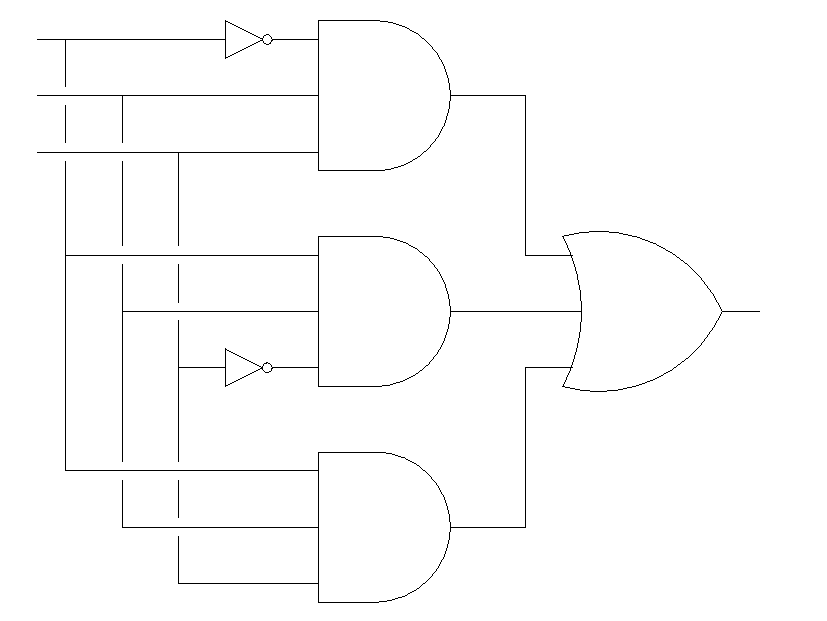
\includegraphics{./logic_circuit.pdf}%
\end{picture}%
\setlength{\unitlength}{3947sp}%
%
\begingroup\makeatletter\ifx\SetFigFont\undefined%
\gdef\SetFigFont#1#2#3#4#5{%
  \reset@font\fontsize{#1}{#2pt}%
  \fontfamily{#3}\fontseries{#4}\fontshape{#5}%
  \selectfont}%
\fi\endgroup%
\begin{picture}(6602,4952)(975,-5237)
\put(1126,-661){\makebox(0,0)[lb]{\smash{{\SetFigFont{12}{14.4}{\familydefault}{\mddefault}{\updefault}{\color[rgb]{0,0,0}x}%
}}}}
\put(1126,-1111){\makebox(0,0)[lb]{\smash{{\SetFigFont{12}{14.4}{\familydefault}{\mddefault}{\updefault}{\color[rgb]{0,0,0}y}%
}}}}
\put(1126,-1561){\makebox(0,0)[lb]{\smash{{\SetFigFont{12}{14.4}{\familydefault}{\mddefault}{\updefault}{\color[rgb]{0,0,0}z}%
}}}}
\put(7126,-2836){\makebox(0,0)[lb]{\smash{{\SetFigFont{12}{14.4}{\familydefault}{\mddefault}{\updefault}{\color[rgb]{0,0,0}out}%
}}}}
\end{picture}%

\end{center}
\caption[Disjunctive normal form.]{A digital logic circuit built % 
using disjunctive normal form.  The output of this circuit is %
$({\lnot}x \land y \land z) \lor (x \land y \land {\lnot}z) \lor (x \land y \land z)$.}
\label{fig:dnf}
\end{figure}

\newpage

\noindent{\large \bf Exercises --- \thesection\ }

\begin{enumerate}

\item Design a digital logic circuit (using and, or \& not gates) that 
implements an exclusive or.

\wbvfill

\hint{First, it's essential to know what is meant by the term "exclusive or". This is the interpretation that many people give to the word "or" -- where "X or Y" means either X is true or Y is true, but that it isn't the case that both X and Y are true. This (wrong) understanding of what "or" means is common because it is often the case that X and Y represent complimentary possibilities: old or new, cold or hot, right or wrong... The truth table for exclusive or (often written xor, pronounced "ex-or", symbolically it is usually $\oplus$) is

\begin{tabular}{|c|c|c|} \hline
\rule[-8pt]{0pt}{30pt}$X$ & $Y$ & $X \,\oplus\, Y$ \\ \hline
\rule[-8pt]{0pt}{30pt}$T$ & $T$ & $\phi$ \\ \hline
\rule[-8pt]{0pt}{30pt}$T$ & $\phi$ & $T$ \\ \hline
\rule[-8pt]{0pt}{30pt}$\phi$ & $T$ & $T$ \\ \hline
\rule[-8pt]{0pt}{30pt}$\phi$ & $\phi$ & $\phi$  \\ \hline
\end{tabular}

\noindent So it's true when one, or the other, but not both of its inputs are true.  The upshot of the last sentence is that we can write $X \oplus Y \; \equiv \; (X \lor Y) \land {\lnot}(X \land Y)$.

The above reformulation should help\ldots 

\vfill

}

\workbookpagebreak

\item Consider the sentence 
``This is a sentence which does not refer to itself.''
which was given in the beginning of this chapter as an example.
Is this sentence a statement?  If so, what is its truth value?

\hint{The only question in your mind, when deciding whether a sentence is a statement, should be "Does this thing have a definite truth value?"
Well?

Isn't it just plainly false?}

%\vspace{.5in}
\vfill

\item Consider the sentence ``This sentence is false.''  Is this 
sentence a statement?

\hint{Try to justify why this sentence can't be either true or false.}

\hintspagebreak

%\vspace{.5in}
\vfill

\workbookpagebreak

\item Complete truth tables for each of the sentences 
$(A \land B) \lor C$ and
$A \land (B \lor C)$.  Does it seem that these sentences have
the same logical content?

\hint{

\vfill

A tiny hint here: since the sentences involve 3 variables you'll need truth tables with 8 rows. Here's a template.

\vfill

\begin{tabular}{|c|c|c|c|c|} \hline
\rule[-8pt]{0pt}{30pt}$A$ & $B$ & $C$ & $(A \land B) \lor C$ & $A \land (B \lor C)$ \\ \hline
\rule[-8pt]{0pt}{30pt}$T$ & $T$ & $T$ & \rule{100pt}{0pt} & \rule{100pt}{0pt} \\ \hline
\rule[-8pt]{0pt}{30pt}$T$ & $T$ & $\phi$  & & \\ \hline
\rule[-8pt]{0pt}{30pt}$T$ & $\phi$  & $T$ & & \\ \hline
\rule[-8pt]{0pt}{30pt}$T$ & $\phi$  & $\phi$  & & \\  \hline
\rule[-8pt]{0pt}{30pt}$\phi$  & $T$ & $T$ & & \\ \hline
\rule[-8pt]{0pt}{30pt}$\phi$  & $T$ & $\phi$  & & \\ \hline
\rule[-8pt]{0pt}{30pt}$\phi$  & $\phi$  & $T$ & & \\ \hline
\rule[-8pt]{0pt}{30pt}$\phi$  & $\phi$  & $\phi$  & & \\  \hline
\end{tabular}
}
\vfill

\hintspagebreak
\workbookpagebreak

\item \label{ex:nand_nor} There are two other logical connectives that are
used somewhat less commonly than $\lor$ and $\land$.
These are the \index{Scheffer stroke} Scheffer stroke and the 
\index{Peirce arrow}Peirce arrow
-- written $\vert$ and $\downarrow$, respectively ---  they are 
also known as \index{NAND} NAND and \index{NOR} NOR.

\noindent The truth tables for these connectives are:
\medskip

\begin{tabular}{c|c|c}
$A$ & $B$ & $A \,\vert\, B$ \\ \hline
$T$ & $T$ & $\phi$ \\
$T$ & $\phi$ & $T$ \\
$\phi$ & $T$ & $T$ \\
$\phi$ & $\phi$ & $T$ 
\end{tabular}
\hspace{.25 in} and \hspace{.25 in}
\begin{tabular}{c|c|c}
$A$ & $B$ & $A \downarrow B$ \\ \hline
$T$ & $T$ & $\phi$ \\
$T$ & $\phi$ & $\phi$ \\
$\phi$ & $T$ & $\phi$ \\
$\phi$ & $\phi$ & $T$ 
\end{tabular}
\medskip

Find an expression for $(A\, \land {\lnot}B) \lor C$
using only these new connectives (as well as negation and the
variable symbols themselves).


\hint{Sorry, I know this is probably the hardest problem in the chapter, but I'm (mostly) not going to help...
Just one hint to help you get started: NAND and NOR are the negations of AND and OR (respectively) so, for example, $(X \land Y) \; \equiv \; {\lnot}(A \,\vert\, B)$.}

\textbookpagebreak
\workbookpagebreak


\item \label{IKK} The famous logician \index{Smullyan, Raymond} Raymond Smullyan devised 
a family of logical puzzles around a fictitious place he called 
\index{Knights and Knaves} ``the Island of Knights and Knaves.''  The inhabitants of the island are either knaves, who always make false statements, or knights, who always make truthful statements.  

In the most famous knight/knave puzzle, you are in a room which has only two exits.  One leads to certain death and the other to freedom.  There are two 
individuals in the room, and you know that one of them is a knight and the other is a knave, but you don't know which.   Your challenge is to determine the door which leads to freedom by asking a single question.

\hint{Ask one of them what the other one would say to do.}

\end{enumerate}


\newpage

\section{Implication}
\label{sec:impl}

Suppose a mother makes the following statement to her child:
``If you finish your peas, you'll get dessert.''

This is a compound sentence made up of the two simpler
sentences $P=$ ``You finish your peas'' and $D=$ ``You'll get dessert.''
It is an example of a type of compound sentence called a 
\index{conditional statement}{\em conditional}.  Conditionals are if-then type statements.  
In ordinary language the word ``then'' is often elided (as is the case
with our example above).  Another way of phrasing the ``If P then D.'' 
relationship is to use the word ``implies'' --- although it would be
a rather uncommon mother who would say ``Finishing your peas implies
that you will receive dessert.'' 

As was the case in the previous section, there are four possible
situations and we must consider each to decide the truth/falsity 
of this conditional statement.  The peas may or may not be finished,
and independently, the dessert may or may not be proffered.   

Suppose the child finishes the peas and the mother comes across
with the dessert.  Clearly, in this situation the mother's statement 
was true.  On the other hand, if the child finishes the hated peas
and yet does not receive a treat, it is just as obvious that the 
mother has lied! 
What do we say about the mother's veracity in the case that the peas
go unfinished?  Here, Mom gets a break.  She can either hold firm
and deliver no dessert, or she can be a softy and give out unearned 
sweets -- in either case, we can't accuse her of telling a falsehood.
The statement she made had to do {\em only} with the eventualities
following total pea consumption, she said nothing about what happens
if the peas go uneaten.

A conditional statement's components are called the 
\index{antecedent}{\em antecedent} 
(this is the ``if'' part, as in ``finish
your peas'') and the \index{consequent}{\em consequent} (this is the ``then'' part, as in
``get dessert'').  The discussion in the 
last paragraph was intended to make the point that when the antecedent
is false, we should consider the conditional to be true.  Conditionals
that are true because their antecedents are false are said to
be \index{vacuous truth}{\em vacuously true}.  The conditional 
involving an antecedent $A$
and a consequent $B$ is expressed symbolically using an arrow: 
$A \implies B$.  Here is a truth table for this connective.

\begin{center}
\begin{tabular}{c|c||c}
\; $A$ \; & \; $B$ \; & \; $A \implies B$ \; \\ \hline
T & T & T \\
T & $\phi$ & $\phi$\\
 $\phi$ & T & T \\
 $\phi$ &  $\phi$ & T\\
\end{tabular}
\end{center}

\begin{exer} 
Note that this truth table is similar to the truth table for
$A \lor B$ in that there is only a single row having a $\phi$ in
the last column.  For $A \lor B$ the $\phi$ occurs in the 4th row
and for $A \implies B$ it occurs in the 2nd row.  This suggests
that by suitably modifying things (replacing $A$ or $B$ by their
negations) we could come up with an ``or'' statement that had the 
same meaning as the conditional.  Try it!
\end{exer}

It is fairly common that conditionals are used to express threats,
as in the peas/dessert example.  Another common way to express a 
threat is to use a disjunction -- ``Finish your peas, or you won't
get dessert.''  If you've been paying attention (and did the last
exercise), you will notice that this is {\em  not} the disjunction
that should have the same meaning as the original conditional.  
There is probably no mother on Earth who would say
``Don't finish your peas, or you get dessert!'' to her child
(certainly not if she expects to be understood).  So what's going on
here?

The problem is that ``Finish your peas, or you won't
get dessert.'' has the same logical content as
``If you get dessert then you finished your peas.''
(Notice that the roles of the antecedent and consequent have been
switched.)  And, while this last sentence sounds awkward, it is
probably a more accurate reflection of what the mother intended.
The problem {\em really} is that people are incredibly sloppy 
with their conditional statements!  A lot of people secretly want 
the 3rd row of the truth table for $\implies$ to have a $\phi$
in it, and it simply doesn't!  The operator that results if we do
make this modification is called the \index{biconditional}
biconditional, and is expressed
in English using the phrase ``if and only if'' (which leads mathematicians
to the abbreviation \index{iff}``iff'' much to the consternation of 
spell-checking programs everywhere).  The biconditional is denoted 
using an arrow that points both ways.  Its truth table follows.

\begin{center}
\begin{tabular}{c|c||c}
\; $A$ \; & \; $B$ \; & \; $A \iff B$ \; \\ \hline
T & T & T \\
T & $\phi$ & $\phi$\\
 $\phi$ & T & $\phi$ \\
 $\phi$ &  $\phi$ & T\\
\end{tabular}
\end{center}

Please note, that while we like to strive for precision, we do not
necessarily recommend the use of phrases such as 
``You will receive dessert if, and only if,
you finish your peas.'' with young children.


Since conditional sentences are often confused with the sentence
that has the roles of antecedent and consequent reversed, this
switched-around sentence has been given a name: it is the 
\index{converse}{\em converse}
of the original statement.  Another conditional that is distinct from 
(but related to) a given conditional is its \index{inverse}{\em inverse}.  
This sort of sentence probably had to be named because of a very common 
misconception, many people think that the way to negate an if-then 
proposition is to negate
its parts.  Algebraically, this looks reasonable -- sort of a distributive
law for logical negation over implications -- ${\lnot}( A \implies B) =
{\lnot}A \implies {\lnot}B$.  Sadly, this reasonable looking assertion
can't possibly be true; since implications have just one $\phi$ in a truth 
table, the negation of an implication  must have three -- but the statement 
with the $\lnot$'s on the {\em parts} of the implication is going to only have 
a single $\phi$ in {\em its} truth table.

To recap, the converse of an implication has the pieces (antecedent and 
consequent) switched about.  The inverse of an implication has the 
pieces negated.  Neither of these is the same as the original implication.
Oddly, this is one of those times when two wrongs {\em do} make a right.
If you start with an implication, form its converse, then take the inverse
of that, you get a statement having exactly the same logical meaning
as the original.  This new statement is called the 
\index{contrapositive}{\em contrapositive}.

This information is displayed in Table~\ref{tab:contra} 

\begin{table}[hbt] 
\begin{center}
\begin{tabular}{cc} 
 & converses \\
 & %
\ifx\pdfoutput\undefined % We're not running pdftex
 
\includegraphics{figures/horiz_arrows.eps} \\%
\else
 
\includegraphics{figures/horiz_arrows.pdf} \\%
\fi
\parbox[c]{10pt}{ \begin{sideways} inverses \end{sideways} } 
\parbox[c]{10pt}{ 
\ifx\pdfoutput\undefined % We're not running pdftex
 
\includegraphics{figures/vert_arrows.eps}% 
\else

\includegraphics{figures/vert_arrows.pdf}% 
\fi } & %
\begin{tabular}{|ccc|ccc|} \hline
 \rule{20pt}{0pt} & \rule{0pt}{20pt} & \rule{20pt}{0pt} & \rule{20pt}{0pt} & \rule{0pt}{20pt} & \rule{20pt}{0pt} \\
 & $A \implies B$ & & & $B \implies A$ & \\
 \rule{0pt}{20pt} & & & & & \\ \hline
 \rule{0pt}{20pt} & & & & & \\
 & ${\lnot}A \implies {\lnot}B$ & & & ${\lnot}B \implies {\lnot}A$ & \\ 
\rule{0pt}{20pt} & & & & & \\ \hline
\end{tabular} \\
\end{tabular}
\end{center}
\caption[Converse, inverse and contrapositive.]{The relationship %
between a conditional statement, its converse, its inverse and its %
contrapositive.}
\label{tab:contra}
\end{table}


One final piece of advice about conditionals: don't confuse logical
if-then relationships with causality.  Many of the if-then sentences
we run into in ordinary life describe cause and effect:  
``If you cut the green wire the bomb will explode.''  (Okay, that one
is an example from the ordinary life of a bomb squad technician, but \ldots)
It is usually best to think of the if-then relationships we find in
Logic as divorced from the flow of time, the fact that $A \implies B$
is logically the same as ${\lnot}A \lor B$ lends credence to this point of view.

\newpage

\noindent{\large \bf Exercises --- \thesection\ }

\begin{enumerate}

\item The transitive property of equality says that if $a=b$ and $b=c$
then $a=c$.  Does the implication arrow satisfy a transitive property?
If so, state it.

\wbvfill

\hint{
I sometimes like to rephrase the implication $X \implies Y$ as ``X's truth forces Y to be true.''  Does that help?
If we know that X being true forces Y to be true, and we also know that Y being true will force Z to be true, what can we conclude?

\vfill

}

\item Complete truth tables for the compound sentences $A \implies B$ and
  ${\lnot}A \lor B$.
  
  \wbvfill
  
\hint{
You should definitely be able to do this one on your own, but anyway, here's an outline of the table:

\begin{tabular}{|c|c|c|c|} \hline
\rule[-6pt]{0pt}{24pt}  $A$ & $B$ & $A \implies B$ & ${\lnot}A \lor B$ \\ \hline
\rule[-6pt]{0pt}{24pt}  $T$ &  $T$ & & \\ \hline
\rule[-6pt]{0pt}{24pt}  $T$ & $\phi$ & & \\ \hline	 	 
\rule[-6pt]{0pt}{24pt}  $\phi$ & $T$ & & \\ \hline
\rule[-6pt]{0pt}{24pt}  $\phi$ & $\phi$ & & \\ \hline
\end{tabular}

\vfill

}

\item Complete a truth table for the compound sentence $A \implies (B \implies C)$ and for the sentence $(A \implies B) \implies C$.  What can you conclude
about conditionals and the associative property?

\wbvfill

\hint{
No help on this one other than to say that the associative property {\bf does not} hold for implications.

\vfill

}

\workbookpagebreak
\hintspagebreak

\item Determine a sentence using the {\em and} connector ($\land$) that
gives the negation of $A \implies B$.

\wbvfill

\hint{Hmmm\ldots This will seem like a strange hint, but if you were to hear a kid at the playground say ``Oh yeah? Well, I did call your mom a fatty and you still haven't clobbered me! Owww! OWWW!!! Stop hitting me!!''

What conditional sentence was he attempting to negate?
}

\item Rewrite the sentence ``Fix the toilet or I won't pay the rent!'' as
a conditional.

\wbvfill

\hint{The way I see it there are eight possible ways to arrange "You fix the toilet" and "I'll pay the rent" (or their respective negations) around an implication arrow.
Here they all are. You decide which one sounds best.

If you fix the toilet, then I'll pay the rent.\newline
If you fix the toilet, then I won't pay the rent.\newline
If you don't fix the toilet, I'll pay the rent.\newline
If you don't fix the toilet, then I won't pay the rent.\newline
If I payed the rent, then you must have fixed the toilet.\newline
If I payed the rent, then you must not have fixed the toilet.\newline
If I didn't pay the rent, then you must have fixed the toilet.\newline
If I didn't pay the rent, then you must not have fixed the toilet.\newline

Some of those are truly strange\ldots
}
\item Why is it that the sentence ``If pigs can fly, I am the king
of Mesopotamia.'' true?

\wbvfill

\hint{Unless we're talking about some celebrity bringing their pet Vietnamese pot-bellied pig into first class with them, or possibly a catapult of some type... The antecedent (the if part) is false, so Yay! I AM the king of Mesopotamia!! Whoo-hooh! What? I'm not? Oh. But the if-then sentence is true. Bummer.}

\item Express the statement $A \implies B$ using the Peirce arrow and/or the
Scheffer stroke. (See Exercise~\ref{ex:nand_nor} in the previous section.)

\wbvfill

\hint{You'll want to use $\vert$, the Scheffer stroke, aka NAND, because it's truth table contains three $T$'s and one $\phi$ -- you'll just need to figure out which of its inputs to negate so as to make that one $\phi$ occur in the second row of the table instead of the first.}

\workbookpagebreak

\item Find the contrapositives of the following sentences.
  \begin{enumerate}
  \item If you can't do the time, don't do the crime.
  \item If you do well in school, you'll get a good job.
  \item If you wish others to treat you in a certain way, you must 
    treat others in that fashion.
  \item If it's raining, there must be clouds.
  \item If $a_n \leq b_n$, for all $n$ and $\sum_{n=0}^\infty b_n$ is a 
convergent series, then $\sum_{n=0}^\infty a_n$ is a convergent series.
  \end{enumerate}

\wbvfill

\hint{
\begin{enumerate}
\item If you do the crime, you must do the time.
\item If you don't have a good job, you must've done poorly in school.
\item If you don't treat others in a certain way, you can't hope for others to treat you in that fashion,
\item If there are no clouds, it can't be raining.
\item If  $\sum_{n=0}^\infty a_n$ is not a convergent series, then either $a_n \leq b_n$, for some $n$ or 
$\sum_{n=0}^\infty b_n$ is not a convergent series.
\end{enumerate}
}
\rule{0pt}{0pt}

\wbvfill

\item What are the converse and inverse of ``If you watch my back, I'll 
watch your back.''?

\wbvfill

\hint{
The converse is ``If I watch your back, then you'll watch my back.''  (Sounds a little dopey doesn't it -- likes its sort of a wishful thinking\ldots)
The inverse is ``If you don't watch my back, then I won't watch your back.''  (Sounds less vapid, but it means the same thing\ldots)
}

\workbookpagebreak

\item The integral test in Calculus is used to determine whether an
infinite series converges or diverges:   Suppose that $f(x)$ is a positive,
decreasing, 
real-valued function with $\lim_{x \longrightarrow \infty} f(x) = 0$, if
the improper integral
$\int_0^\infty f(x)$ has a finite value, then the infinite series 
$\sum_{n=1}^\infty f(n)$ converges.

The integral test should be envisioned by letting the series correspond
to a right-hand Riemann sum for the integral, since the function is decreasing,
a right-hand Riemann sum is an underestimate for the value of the integral,
thus

\[ \sum_{n=1}^\infty f(n) < \int_0^\infty f(x). \]

Discuss the meanings of and (where possible) provide justifications for
the inverse, converse and contrapositive of the conditional statement 
in the integral test.

\wbvfill

\hint{
The inverse says -- if the integral isn't finite, then the series doesn't converge. You can cook-up a function that shows this to be false by (for example) creating one with vertical asymptotes that occur in between the integer $x$-values. Even one such pole can be enough to make the integral go infinite.
The converse says that if the series converges, the integral must be finite. The counter-example we just discussed would work here too.

The contrapositive says that if the series doesn't converge, then the integral must not be finite. If we were allowed to use discontinuous functions, it isn't too hard to come up with an $f$ that actually has zero area under it -- just make f be identically zero except at the integer x-values where it will take the same values as the terms of the series. But wait, the function we just described isn't ``decreasing'' -- which is probably why that hypothesis was put in there!
}

\workbookpagebreak

\item On the Island of Knights and Knaves (see page~\pageref{IKK}) you encounter two individuals named Locke and Demosthenes.  

Locke says, ``Demosthenes is a knave.'' \newline
Demosthenes says ``Locke and I are knights.''

Who is a knight and who a knave?

\wbvfill

\hint{Could Demosthenes be telling the truth?}

\end{enumerate}


\newpage

\section{Logical equivalences}
\label{sec:le}

Some logical statements are ``the same.''  For example, in the last
section, we discussed the fact that a conditional
and its contrapositive have the same logical content.  Wouldn't
we be justified in writing something like the following?

\[ A \implies B \; = \; {\lnot}B \implies {\lnot}A \]

Well, one pretty serious objection to doing that is that the 
equals sign ($=$) has already got a job; it is used to indicate that
two numerical quantities are the same.  What we're doing here is 
really sort of a different thing!  Nevertheless, there is a concept
of ``sameness'' between certain compound statements, and we need a 
symbolic way of expressing it.  There are two notations in common 
use.  The notation that seems to be preferred by logicians is the
biconditional ($\iff$).  The notation we'll use
in the rest of this book is an equals sign with a bit of extra decoration
on it ($\cong$).  

Thus we can can either write 

\[ (A \implies B) \; \iff \; ({\lnot}B \implies {\lnot}A) \]

\noindent or 

\[ A \implies B \; \cong \; {\lnot}B \implies {\lnot}A. \]

\noindent I like the latter, but use whichever form you like -- no one
will have any problem understanding either.

The formal definition of \index{logical equivalence}{\em logical equivalence}, 
which is what we've
been describing, is this:  two compound sentences are logically equivalent
if in a truth table (that contains all possible combinations of the 
truth values of the predicate variables in its rows) the truth values
of the two sentences are equal in every row. 

\begin{exer} 
Consider the two compound sentences $A \lor B$ and $A \lor ({\lnot}A \land B)$.
There are a total of 2 predicate variables between them, so a truth table
with 4 rows will suffice.  Fill out the missing entries in the truth
table and determine whether the statements are equivalent.

\begin{center}
\begin{tabular}{c|c||c|c}
\; $A$ \; & \; $B$ \; & \; $A \lor B$ \; & \; $A \lor ({\lnot}A \land B)$\; \\ \hline
T & T &  & \\
T & $\phi$ & & \\
 $\phi$ & T & &  \\
 $\phi$ &  $\phi$  & &\\
\end{tabular}
\end{center}

\end{exer}

One could, in principle, verify all logical equivalences by filling out
truth tables.  Indeed, in the exercises for this section we will ask you
to develop a certain facility at this task.  While this activity can
be somewhat fun, and many of my students want the filling-out of truth 
tables to
be a significant portion of their midterm exam, you will probably eventually
come to find it somewhat tedious.  A slightly more mature approach to logical
equivalences is this: use a set of basic equivalences -- which themselves
may be verified via truth tables -- as the basic {\em rules} or 
\index{laws of logical equivalence}{\em laws}
of logical equivalence, and develop a strategy for converting one
sentence into another using these rules.  This process will feel very
familiar, it is like ``doing'' algebra, but the rules one is allowed 
to use are subtly different.

First we have the \index{commutative law}{\em commutative laws}, 
one each for conjunction
and disjunction.  It's worth noting that there {\em isn't} a commutative
law for implication.   

The commutative property of conjunction says that $A \land B \cong B \land A$.
This is quite an apparent statement from the perspective of linguistics.
Surely it's the same thing to say ``the weather is cold and snowy'' as it is to
say ``the weather is snowy and cold.''   
This commutative property is also clear 
from the perspective of digital logic circuits.

\begin{center}
\begin{picture}(0,0)%
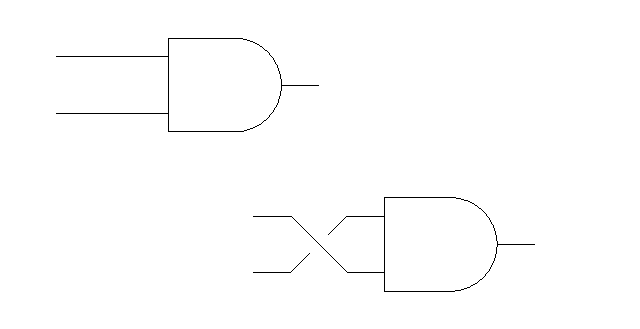
\includegraphics{./comm_conj.pdf}%
\end{picture}%
\setlength{\unitlength}{3947sp}%
%
\begingroup\makeatletter\ifx\SetFigFont\undefined%
\gdef\SetFigFont#1#2#3#4#5{%
  \reset@font\fontsize{#1}{#2pt}%
  \fontfamily{#3}\fontseries{#4}\fontshape{#5}%
  \selectfont}%
\fi\endgroup%
\begin{picture}(5102,2627)(1125,-2987)
\put(2926,-2611){\makebox(0,0)[lb]{\smash{{\SetFigFont{12}{14.4}{\familydefault}{\mddefault}{\updefault}{\color[rgb]{0,0,0}$B$}%
}}}}
\put(2926,-2161){\makebox(0,0)[lb]{\smash{{\SetFigFont{12}{14.4}{\familydefault}{\mddefault}{\updefault}{\color[rgb]{0,0,0}$A$}%
}}}}
\put(5476,-2386){\makebox(0,0)[lb]{\smash{{\SetFigFont{12}{14.4}{\familydefault}{\mddefault}{\updefault}{\color[rgb]{0,0,0}$B \land A$}%
}}}}
\put(3751,-1111){\makebox(0,0)[lb]{\smash{{\SetFigFont{12}{14.4}{\familydefault}{\mddefault}{\updefault}{\color[rgb]{0,0,0}$A \land B$}%
}}}}
\put(1351,-1336){\makebox(0,0)[lb]{\smash{{\SetFigFont{12}{14.4}{\familydefault}{\mddefault}{\updefault}{\color[rgb]{0,0,0}$B$}%
}}}}
\put(1351,-886){\makebox(0,0)[lb]{\smash{{\SetFigFont{12}{14.4}{\familydefault}{\mddefault}{\updefault}{\color[rgb]{0,0,0}$A$}%
}}}}
\end{picture}%

\end{center}   
  
The commutative property of disjunctions is equally transparent from
the perspective of a circuit diagram.  

\begin{center}
\begin{picture}(0,0)%
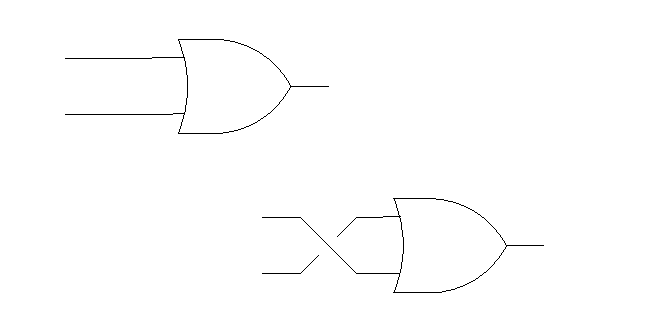
\includegraphics{figures/comm_disj.pdf}%
\end{picture}%
\setlength{\unitlength}{3947sp}%
%
\begingroup\makeatletter\ifx\SetFigFont\undefined%
\gdef\SetFigFont#1#2#3#4#5{%
  \reset@font\fontsize{#1}{#2pt}%
  \fontfamily{#3}\fontseries{#4}\fontshape{#5}%
  \selectfont}%
\fi\endgroup%
\begin{picture}(5177,2552)(1050,-2912)
\put(2926,-2611){\makebox(0,0)[lb]{\smash{{\SetFigFont{12}{14.4}{\familydefault}{\mddefault}{\updefault}{\color[rgb]{0,0,0}$B$}%
}}}}
\put(2926,-2161){\makebox(0,0)[lb]{\smash{{\SetFigFont{12}{14.4}{\familydefault}{\mddefault}{\updefault}{\color[rgb]{0,0,0}$A$}%
}}}}
\put(1351,-1336){\makebox(0,0)[lb]{\smash{{\SetFigFont{12}{14.4}{\familydefault}{\mddefault}{\updefault}{\color[rgb]{0,0,0}$B$}%
}}}}
\put(1351,-886){\makebox(0,0)[lb]{\smash{{\SetFigFont{12}{14.4}{\familydefault}{\mddefault}{\updefault}{\color[rgb]{0,0,0}$A$}%
}}}}
\put(3751,-1111){\makebox(0,0)[lb]{\smash{{\SetFigFont{12}{14.4}{\familydefault}{\mddefault}{\updefault}{\color[rgb]{0,0,0}$A \lor B$}%
}}}}
\put(5476,-2386){\makebox(0,0)[lb]{\smash{{\SetFigFont{12}{14.4}{\familydefault}{\mddefault}{\updefault}{\color[rgb]{0,0,0}$B \lor A$}%
}}}}
\end{picture}%

\end{center}   
  
The \index{associative law}{\em associative laws} also have something to do with what order operations
are done.  One could think of the difference in the following terms:  
Commutative properties
involve spatial or physical order and the associative properties involve
temporal order.  The associative law of addition could be used to say we'll
get the same result if we add 2 and 3 first, then add 4, or if we add 2 to the 
sum of 3 and 4 (i.e. that $(2+3)+4$ is the same as $2+(3+4)$.)  Note that 
physically, the numbers are in the same order (2 then 3 then 4) in both 
expressions but that the parentheses indicate a precedence in {\em when} the
plus signs are evaluated. 

The associative law of conjunction states that $A \land (B \land C) \cong
(A \land B) \land C$.  In visual terms, this means the following two 
circuit diagrams are equivalent.

\begin{center}
\begin{picture}(0,0)%
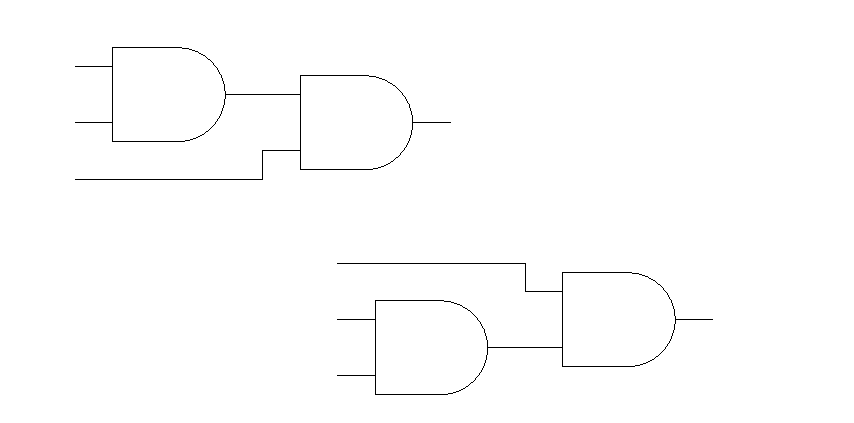
\includegraphics{./assoc_conj.pdf}%
\end{picture}%
\setlength{\unitlength}{3947sp}%
%
\begingroup\makeatletter\ifx\SetFigFont\undefined%
\gdef\SetFigFont#1#2#3#4#5{%
  \reset@font\fontsize{#1}{#2pt}%
  \fontfamily{#3}\fontseries{#4}\fontshape{#5}%
  \selectfont}%
\fi\endgroup%
\begin{picture}(6827,3377)(225,-3437)
\put(601,-661){\makebox(0,0)[lb]{\smash{{\SetFigFont{12}{14.4}{\familydefault}{\mddefault}{\updefault}{\color[rgb]{0,0,0}$A$}%
}}}}
\put(601,-1111){\makebox(0,0)[lb]{\smash{{\SetFigFont{12}{14.4}{\familydefault}{\mddefault}{\updefault}{\color[rgb]{0,0,0}$B$}%
}}}}
\put(601,-1561){\makebox(0,0)[lb]{\smash{{\SetFigFont{12}{14.4}{\familydefault}{\mddefault}{\updefault}{\color[rgb]{0,0,0}$C$}%
}}}}
\put(3901,-1111){\makebox(0,0)[lb]{\smash{{\SetFigFont{12}{14.4}{\familydefault}{\mddefault}{\updefault}{\color[rgb]{0,0,0}$(A \land B) \land C$}%
}}}}
\put(2701,-2236){\makebox(0,0)[lb]{\smash{{\SetFigFont{12}{14.4}{\familydefault}{\mddefault}{\updefault}{\color[rgb]{0,0,0}$A$}%
}}}}
\put(2701,-2686){\makebox(0,0)[lb]{\smash{{\SetFigFont{12}{14.4}{\familydefault}{\mddefault}{\updefault}{\color[rgb]{0,0,0}$B$}%
}}}}
\put(2701,-3136){\makebox(0,0)[lb]{\smash{{\SetFigFont{12}{14.4}{\familydefault}{\mddefault}{\updefault}{\color[rgb]{0,0,0}$C$}%
}}}}
\put(6001,-2686){\makebox(0,0)[lb]{\smash{{\SetFigFont{12}{14.4}{\familydefault}{\mddefault}{\updefault}{\color[rgb]{0,0,0}$A \land (B \land C)$}%
}}}}
\end{picture}%

\end{center}   
  
The associative law of disjunction states that $A \lor (B \lor C) \cong
(A \lor B) \lor C$.  Visually, this looks like:

\begin{center}
\begin{picture}(0,0)%
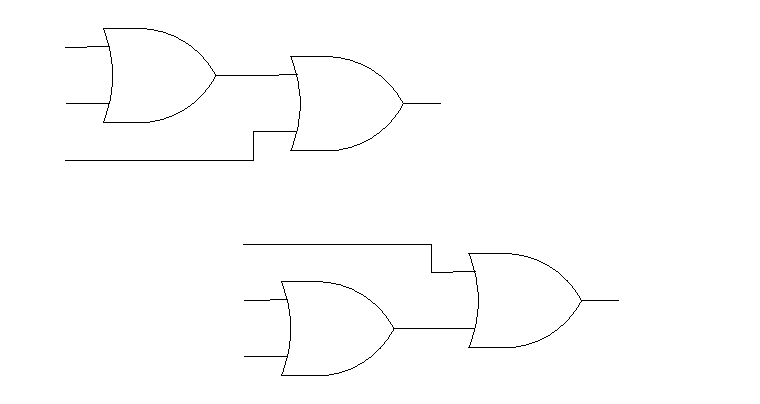
\includegraphics{./assoc_disj.pdf}%
\end{picture}%
\setlength{\unitlength}{3947sp}%
%
\begingroup\makeatletter\ifx\SetFigFont\undefined%
\gdef\SetFigFont#1#2#3#4#5{%
  \reset@font\fontsize{#1}{#2pt}%
  \fontfamily{#3}\fontseries{#4}\fontshape{#5}%
  \selectfont}%
\fi\endgroup%
\begin{picture}(6077,3227)(375,-2987)
\put(676,-211){\makebox(0,0)[lb]{\smash{{\SetFigFont{12}{14.4}{\familydefault}{\mddefault}{\updefault}{\color[rgb]{0,0,0}$A$}%
}}}}
\put(676,-661){\makebox(0,0)[lb]{\smash{{\SetFigFont{12}{14.4}{\familydefault}{\mddefault}{\updefault}{\color[rgb]{0,0,0}$B$}%
}}}}
\put(676,-1111){\makebox(0,0)[lb]{\smash{{\SetFigFont{12}{14.4}{\familydefault}{\mddefault}{\updefault}{\color[rgb]{0,0,0}$C$}%
}}}}
\put(3976,-661){\makebox(0,0)[lb]{\smash{{\SetFigFont{12}{14.4}{\familydefault}{\mddefault}{\updefault}{\color[rgb]{0,0,0}$(A \lor B) \lor C$}%
}}}}
\put(2101,-1786){\makebox(0,0)[lb]{\smash{{\SetFigFont{12}{14.4}{\familydefault}{\mddefault}{\updefault}{\color[rgb]{0,0,0}$A$}%
}}}}
\put(2101,-2236){\makebox(0,0)[lb]{\smash{{\SetFigFont{12}{14.4}{\familydefault}{\mddefault}{\updefault}{\color[rgb]{0,0,0}$B$}%
}}}}
\put(2101,-2686){\makebox(0,0)[lb]{\smash{{\SetFigFont{12}{14.4}{\familydefault}{\mddefault}{\updefault}{\color[rgb]{0,0,0}$C$}%
}}}}
\put(5401,-2236){\makebox(0,0)[lb]{\smash{{\SetFigFont{12}{14.4}{\familydefault}{\mddefault}{\updefault}{\color[rgb]{0,0,0}$A \lor (B \lor C)$}%
}}}}
\end{picture}%

\end{center}   
  

\begin{exer}
In a situation where {\em both} associativity and commutativity pertain
the symbols involved can appear in any order and with any reasonable 
parenthesization.  In how many different ways can the sum $2+3+4$ 
be expressed?  Only consider expression that are fully parenthesized.
\end{exer}
 
The next type of basic logical equivalences we'll consider are the
so-called \index{distributive law}{\em distributive laws}.  
Distributive laws involve the 
interaction of two operations, when we distribute multiplication 
over a sum, we effectively replace one instance of an operand {\em 
and the associated operator}, with two instances, as is illustrated
below.

\begin{center}
\begin{picture}(0,0)%
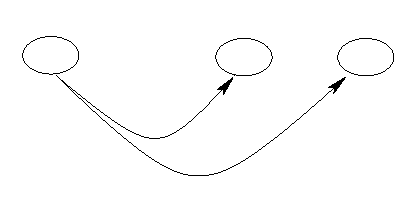
\includegraphics{./dist_2x3+4.pdf}%
\end{picture}%
\setlength{\unitlength}{3947sp}%
%
\begingroup\makeatletter\ifx\SetFigFont\undefined%
\gdef\SetFigFont#1#2#3#4#5{%
  \reset@font\fontsize{#1}{#2pt}%
  \fontfamily{#3}\fontseries{#4}\fontshape{#5}%
  \selectfont}%
\fi\endgroup%
\begin{picture}(3227,1577)(1125,-4337)
\put(1426,-3286){\makebox(0,0)[lb]{\smash{{\SetFigFont{12}{14.4}{\familydefault}{\mddefault}{\updefault}{\color[rgb]{0,0,0}2  *  ( 3 + 4 ) = ( 2  *  3 ) + ( 2  *  4 )}%
}}}}
\end{picture}%

\end{center}   
  
The logical operators $\land$ and $\lor$ each distribute over the other.
Thus we have the distributive law of conjunction over disjunction, which
is expressed in the equivalence 
$A \land (B \lor C) \cong (A \land B) \lor (A \land C)$ 
and in the following digital logic circuit diagram.

\begin{center}
\begin{picture}(0,0)%
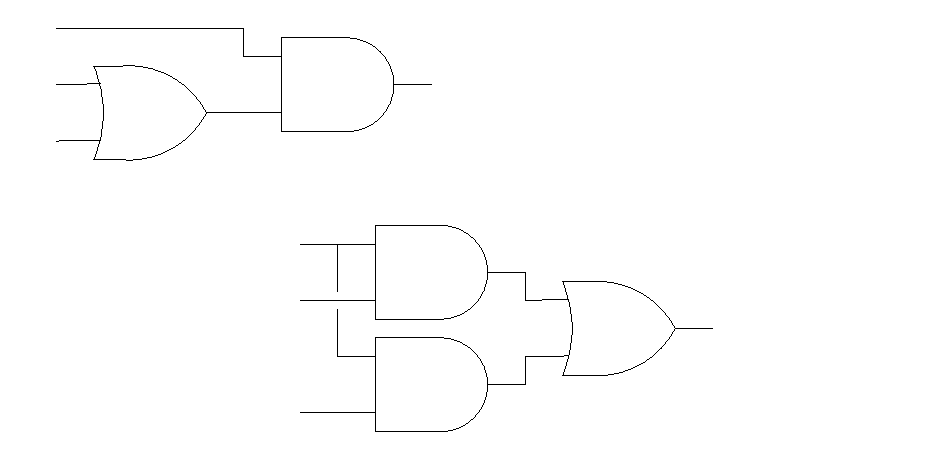
\includegraphics{./dist_and_o_or.pdf}%
\end{picture}%
\setlength{\unitlength}{3947sp}%
%
\begingroup\makeatletter\ifx\SetFigFont\undefined%
\gdef\SetFigFont#1#2#3#4#5{%
  \reset@font\fontsize{#1}{#2pt}%
  \fontfamily{#3}\fontseries{#4}\fontshape{#5}%
  \selectfont}%
\fi\endgroup%
\begin{picture}(7427,3677)(600,-3737)
\put(826,-1261){\makebox(0,0)[lb]{\smash{{\SetFigFont{12}{14.4}{\familydefault}{\mddefault}{\updefault}{\color[rgb]{0,0,0}$C$}%
}}}}
\put(826,-811){\makebox(0,0)[lb]{\smash{{\SetFigFont{12}{14.4}{\familydefault}{\mddefault}{\updefault}{\color[rgb]{0,0,0}$B$}%
}}}}
\put(826,-361){\makebox(0,0)[lb]{\smash{{\SetFigFont{12}{14.4}{\familydefault}{\mddefault}{\updefault}{\color[rgb]{0,0,0}$A$}%
}}}}
\put(4126,-811){\makebox(0,0)[lb]{\smash{{\SetFigFont{12}{14.4}{\familydefault}{\mddefault}{\updefault}{\color[rgb]{0,0,0}$A \land (B \lor C)$}%
}}}}
\put(2776,-2086){\makebox(0,0)[lb]{\smash{{\SetFigFont{12}{14.4}{\familydefault}{\mddefault}{\updefault}{\color[rgb]{0,0,0}$A$}%
}}}}
\put(2776,-2536){\makebox(0,0)[lb]{\smash{{\SetFigFont{12}{14.4}{\familydefault}{\mddefault}{\updefault}{\color[rgb]{0,0,0}$B$}%
}}}}
\put(2776,-3436){\makebox(0,0)[lb]{\smash{{\SetFigFont{12}{14.4}{\familydefault}{\mddefault}{\updefault}{\color[rgb]{0,0,0}$C$}%
}}}}
\put(6376,-2761){\makebox(0,0)[lb]{\smash{{\SetFigFont{12}{14.4}{\familydefault}{\mddefault}{\updefault}{\color[rgb]{0,0,0}$(A \land B) \lor (A \land C)$}%
}}}}
\end{picture}%

\end{center}   

We also have the distributive law of disjunction over conjunction 
which is given by the equivalence 
$A \lor (B \land C) \cong (A \lor B) \land (A \lor C)$ and in the 
circuit diagram:

\begin{center}
\begin{picture}(0,0)%
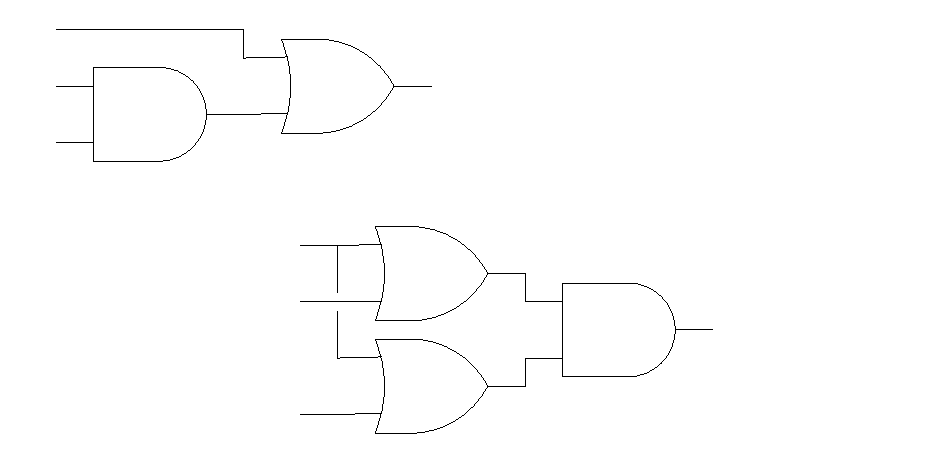
\includegraphics{./dist_or_o_and.pdf}%
\end{picture}%
\setlength{\unitlength}{3947sp}%
%
\begingroup\makeatletter\ifx\SetFigFont\undefined%
\gdef\SetFigFont#1#2#3#4#5{%
  \reset@font\fontsize{#1}{#2pt}%
  \fontfamily{#3}\fontseries{#4}\fontshape{#5}%
  \selectfont}%
\fi\endgroup%
\begin{picture}(7427,3602)(600,-3662)
\put(2776,-2086){\makebox(0,0)[lb]{\smash{{\SetFigFont{12}{14.4}{\familydefault}{\mddefault}{\updefault}{\color[rgb]{0,0,0}$A$}%
}}}}
\put(2776,-2536){\makebox(0,0)[lb]{\smash{{\SetFigFont{12}{14.4}{\familydefault}{\mddefault}{\updefault}{\color[rgb]{0,0,0}$B$}%
}}}}
\put(2776,-3436){\makebox(0,0)[lb]{\smash{{\SetFigFont{12}{14.4}{\familydefault}{\mddefault}{\updefault}{\color[rgb]{0,0,0}$C$}%
}}}}
\put(6376,-2761){\makebox(0,0)[lb]{\smash{{\SetFigFont{12}{14.4}{\familydefault}{\mddefault}{\updefault}{\color[rgb]{0,0,0}$(A \lor B) \land (A \lor C)$}%
}}}}
\put(826,-1261){\makebox(0,0)[lb]{\smash{{\SetFigFont{12}{14.4}{\familydefault}{\mddefault}{\updefault}{\color[rgb]{0,0,0}$C$}%
}}}}
\put(826,-811){\makebox(0,0)[lb]{\smash{{\SetFigFont{12}{14.4}{\familydefault}{\mddefault}{\updefault}{\color[rgb]{0,0,0}$B$}%
}}}}
\put(826,-361){\makebox(0,0)[lb]{\smash{{\SetFigFont{12}{14.4}{\familydefault}{\mddefault}{\updefault}{\color[rgb]{0,0,0}$A$}%
}}}}
\put(4126,-811){\makebox(0,0)[lb]{\smash{{\SetFigFont{12}{14.4}{\familydefault}{\mddefault}{\updefault}{\color[rgb]{0,0,0}$A \lor (B \land C)$}%
}}}}
\end{picture}%

\end{center}   

Traditionally, the laws we've just stated would be called 
{\em left}-distributive laws and we would also need to state 
that there are {\em right}-distributive laws that apply.  Since,
in the current setting, we have already said that the commutative
law is valid, this isn't really necessary.

\begin{exer}
State the right-hand versions of the distributive laws.
\end{exer}

The next set of laws we'll consider come from trying to
figure out what the distribution of a minus sign over a sum
($-(x+y) = -x + -y$)
should correspond to in Boolean algebra.  At first blush one 
might assume the analogous thing in Boolean algebra would be
something like ${\lnot}(A \land B) \cong {\lnot}A \land {\lnot}B$,
but we can easily dismiss this by looking at a truth table.

\begin{center}
\begin{tabular}{c|c||c|c}
\; $A$ \; & \; $B$ \; & \; ${\lnot}(A \land B)$ \; & \; ${\lnot}A \land {\lnot}B$\; \\ \hline
T & T &  $\phi$ & $\phi$ \\
T & $\phi$ & T & $\phi$ \\
 $\phi$ & T & T & $\phi$ \\
 $\phi$ &  $\phi$  & T & T\\
\end{tabular}
\end{center}

What actually works is a set of rules known as 
\index{DeMorgan's laws}DeMorgan's laws, which
basically say that you distribute the negative sign but
you also must change the operator.  As logical equivalences,
DeMorgan's laws are 

\[ {\lnot}(A \land B) \; \cong \; {\lnot}A \lor {\lnot}B \]

\noindent and

\[ {\lnot}(A \lor B) \; \cong \; {\lnot}A \land {\lnot}B. \]

In ordinary arithmetic there are two notions of ``inverse.''  The 
{\em negative} of a number is known as its additive inverse and
the {\em reciprocal} of a number is its multiplicative inverse.
These notions lead to a couple of equations,

\[ x + -x = 0 \]

\noindent and

\[ x \cdot \frac{1}{x} = 1. \]

\noindent Boolean algebra only has one ``inverse'' concept, the denial
 of a predicate (i.e. logical negation), but the equations above have analogues, as do
the symbols $0$ and $1$ that appear in them.  First, consider
the Boolean expression $A \lor {\lnot}A$.  This is the logical {\em or}
of a statement and its exact opposite; when one is true the other is 
false and vice versa.  But, the disjunction $A \lor {\lnot}A$, is 
always true!  We use the symbol $t$ (which stands for 
\index{tautology}{\em tautology})
to represent a compound sentence whose truth value is always true.
A tautology ($t$) is to Boolean algebra something like a zero ($0$)
is to arithmetic.  Similar thinking about the Boolean expression
  $A \land {\lnot}A$ leads to the definition of the symbol $c$ (which
stands for \index{contradiction}{\em contradiction}) to 
represent a sentence that is always
false.  The rules we have been discussing are known as 
\index{complementarity laws}{\em complementarity laws}:

\[ A \lor {\lnot}A \; \cong \; t \mbox{\rule{12pt}{0pt} and \rule{12pt}{0pt}}
A \land {\lnot}A \; \cong \; c \]


Now that we have the special logical sentences represented by $t$ and $c$
we can present the so-called \index{identity laws}{\em identity laws}, 
$A \land t \cong A$ and
$A \lor c \cong A$.  If you ``and'' a statement with something that is always
true, this new compound has the exact same truth values as the original.
If you ``or'' a statement with something that is always false, the new compound
statement is also unchanged from the original.  Thus performing a 
conjunction with a tautology has no effect -- sort of like multiplying by 1.
Performing a disjunction with a contradiction also has no effect -- this is
somewhat akin to adding 0. 

The number 0 has a special property: $0 \cdot x = 0$ is an equation that 
holds no matter what $x$ is.  This is known as a domination property.  Note 
that there isn't a dominance rule that involves 1.
 On the Boolean side, 
{\em both} the symbols $t$ and $c$ have related domination rules.

\[ A \lor t \cong t \mbox{\rule{12pt}{0pt} and \rule{12pt}{0pt}} 
A \land c \cong c \]
 
In mathematics the word \index{idempotent}{\em idempotent} is used to describe situations where 
a power of a thing may be equal to that thing.  For example, because $(-1)^3 = -1$, we say that $-1$ is an idempotent.  Both of the Boolean operations 
have idempotence relations that just always work (regardless of the operand).
In ordinary algebra idempotents are very rare ($0$, $1$ and $-1$ are the only
ones that come to mind), but in Boolean algebra {\em every} statement
is equivalent to its square -- where the square of $A$ can be interpreted 
either as $A \land A$ or as $A \lor A$.

\[ A \lor A \cong A \mbox{\rule{12pt}{0pt} and \rule{12pt}{0pt}}% 
A \land A \cong A \]

There are a couple of properties of the logical negation operator 
that should be stated, though probably they seem self-evident.
If you form the denial of a denial, you come back to the 
same thing as the original; also the symbols $c$ and $t$ are negations
of one another.

\[ \lnot({\lnot}A) \cong A \mbox{\rule{12pt}{0pt} and \rule{12pt}{0pt}}% 
{\lnot}t  \cong c \] 

Finally, we should mention a really strange property, called 
\index{absorption}{\em absorption},
which states that the expressions $A \land (A \lor B)$ and $A \lor (A \land B)$
don't actually have anything to do with $B$ at all!  Both of the preceding
statements are equivalent to $A$.

\[ A \land (A \lor B) \cong A \mbox{\rule{12pt}{0pt} and \rule{12pt}{0pt}}% 
A \lor (A \land B) \cong A \]

In Table~\ref{tab:bool_equiv}, we have collected all of these basic logical
equivalences in one place.

\begin{table}[hbt] 
\begin{center}
\begin{tabular}{c|c|c|c} 
 & \begin{minipage}{.25\textwidth} \centerline{Conjunctive}
\centerline{\rule[-10pt]{0pt}{10pt}version} \end{minipage} & 
\begin{minipage}{.25\textwidth} \centerline{Disjunctive}
\centerline{\rule[-10pt]{0pt}{10pt}version} \end{minipage} & 
\begin{minipage}{.25\textwidth} \centerline{Algebraic}
\centerline{\rule[-10pt]{0pt}{10pt}analog} \end{minipage} \\ \hline
\begin{minipage}{.25\textwidth} \rule{0pt}{22pt}\index{commutative law}Commutative \\ \rule{12pt}{0pt} laws\rule[-10pt]{0pt}{10pt} \end{minipage} & 
\begin{minipage}{.25\textwidth} \centerline{$A \land B \cong B \land A$} \end{minipage} & 
\begin{minipage}{.25\textwidth} \centerline{$A \lor B \cong B \lor A$} \end{minipage} & 
\begin{minipage}{.25\textwidth} \centerline{$2+3 = 3+2$}  \end{minipage}  \\ \hline
\begin{minipage}{.25\textwidth} \rule{0pt}{22pt}\index{associative law}Associative \\ \rule{12pt}{0pt} laws\rule[-10pt]{0pt}{10pt} \end{minipage} & 
\begin{minipage}{.25\textwidth} \centerline{$A \land (B \land C)$\rule{16pt}{0pt}} 
\centerline{\rule{16pt}{0pt} $\cong (A \land B) \land C $}\end{minipage} &
\begin{minipage}{.25\textwidth} \centerline{$A \lor (B \lor C)$ \rule{16pt}{0pt}}
\centerline{\rule{16pt}{0pt} $\cong (A \lor B) \lor C $} \end{minipage} & 
\begin{minipage}{.25\textwidth} 
\centerline{$2+(3+4) $ \rule{16pt}{0pt}} 
\centerline{\rule{24pt}{0pt} $= (2+3)+4$} \end{minipage} \\ \hline 
\begin{minipage}{.25\textwidth} \rule{0pt}{22pt}\index{distributive law}Distributive \\ \rule{12pt}{0pt} laws\rule[-10pt]{0pt}{10pt} \end{minipage} &  
\begin{minipage}{.25\textwidth} 
\centerline{$A \land (B \lor C) \cong $ \rule{16pt}{0pt}} 
\centerline{$(A \land B) \lor (A \land C)$} \end{minipage} & 
\begin{minipage}{.25\textwidth} \centerline{$A \lor (B \land C) \cong $ \rule{16pt}{0pt}} 
\centerline{$(A \lor B) \land (A \lor C)$} \end{minipage} & 
\begin{minipage}{.25\textwidth} 
\centerline{$2\cdot(3+4) $ \rule{16pt}{0pt}}
\centerline{\rule{16pt}{0pt} $ = (2\cdot 3 + 2\cdot 4)$} \end{minipage} \\ \hline 
\begin{minipage}{.25\textwidth} \rule{0pt}{22pt}\index{DeMorgan's law}DeMorgan's \\ \rule{12pt}{0pt} laws\rule[-10pt]{0pt}{10pt} \end{minipage} & 
\begin{minipage}{.25\textwidth} \centerline{${\lnot}(A \land B)$ \rule{25pt}{0pt}}
\centerline{ \rule{16pt}{0pt} $ \cong \; {\lnot}A \lor {\lnot}B$} \end{minipage} & 
\begin{minipage}{.25\textwidth} \centerline{${\lnot}(A \lor B)$\rule{25pt}{0pt}}
\centerline{ \rule{16pt}{0pt} $\cong \; {\lnot}A \land {\lnot}B$} \end{minipage} & none \\ \hline 
\begin{minipage}{.25\textwidth} \rule{0pt}{22pt}\index{double negation}Double negation \rule[-10pt]{0pt}{10pt}   \end{minipage} & 
\begin{minipage}{.25\textwidth} \centerline{${\lnot}({\lnot}A) \; \cong \; A$}  \end{minipage} & 
\begin{minipage}{.25\textwidth} \centerline{same} \end{minipage} & $-(-2) = 2$ \\ \hline 

\begin{minipage}{.25\textwidth} \rule{0pt}{22pt}\index{complementarity law}Complementarity\rule[-10pt]{0pt}{10pt} \end{minipage} & 
\begin{minipage}{.25\textwidth} \centerline{$A \land {\lnot}A \; \cong \; c$} \end{minipage} & 
\begin{minipage}{.25\textwidth} \centerline{$A \lor {\lnot}A \; \cong \; t$} \end{minipage} &  
\begin{minipage}{.25\textwidth} \centerline{$2 + (-2) = 0$} \end{minipage} \\ \hline 
\begin{minipage}{.25\textwidth} \rule{0pt}{22pt}\index{identity law}Identity \\ \rule{12pt}{0pt} laws\rule[-10pt]{0pt}{10pt} \end{minipage} & 
\begin{minipage}{.25\textwidth} \centerline{$A \land t \cong A$} \end{minipage} & 
\begin{minipage}{.25\textwidth} \centerline{$A \lor c \cong A$} \end{minipage} & 
\begin{minipage}{.25\textwidth} \centerline{$7 + 0 = 7$} \end{minipage}\\ \hline 
\begin{minipage}{.25\textwidth} \rule{0pt}{22pt}\index{domination law}Domination\rule[-10pt]{0pt}{10pt} \end{minipage} & 
\begin{minipage}{.25\textwidth}  \centerline{$A \land c \cong c$} \end{minipage} & 
\begin{minipage}{.25\textwidth} \centerline{$A \lor t \cong t$} \end{minipage} & 
\begin{minipage}{.25\textwidth} \centerline{$7 \cdot 0 = 0$} \end{minipage}\\ \hline
\begin{minipage}{.25\textwidth} \rule{0pt}{22pt}\index{idempotence}Idempotence\rule[-10pt]{0pt}{10pt} \end{minipage} & 
\begin{minipage}{.25\textwidth} \centerline{$A \land A \cong A$} \end{minipage} & 
\begin{minipage}{.25\textwidth} \centerline{$A \lor A \cong A$} \end{minipage} & 
\begin{minipage}{.25\textwidth} \centerline{$ 1 \cdot 1 = 1$} \end{minipage} \\ \hline
\begin{minipage}{.25\textwidth} \rule{0pt}{22pt}\index{absorption}Absorption\rule[-10pt]{0pt}{10pt} \end{minipage} & 
\begin{minipage}{.25\textwidth} \centerline{$A \land (A \lor B) \cong A$} \end{minipage} & 
\begin{minipage}{.25\textwidth} \centerline{$A \lor (A \land B) \cong A$} \end{minipage} & none \\ 
\end{tabular} 
\end{center} 
\caption{Basic logical equivalences. }
\label{tab:bool_equiv}\index{rules of replacement}
\end{table}

\clearpage

\noindent{\large \bf Exercises --- \thesection\ }

\begin{enumerate}

\item There are 3 operations used in basic algebra (addition, 
multiplication and exponentiation) and thus
there are potentially 6 different distributive laws.  State
all 6 ``laws'' and determine which 2 are actually valid.
(As an example, the distributive law of addition over multiplication
would look like $x + (y \cdot z) = (x + y) \cdot (x + z)$, this isn't 
one of the true ones.) 

\wbvfill

\hint{
\vfill

These ``laws'' should probably be layed-out in a big 3 by 3 table. Such a table would of course have 9 cells, but we won't be using the cells on the diagonal because they would involve an operation distributing over itself. (That can't happen, can it?)
I'm going to put a few of the entries in, and you do the rest.

\vfill

\begin{tabular}{c|c|c|c|} 
  & \rule{36pt}{0pt} $+$ \rule{36pt}{0pt} & \rule{36pt}{0pt} $\ast$ \rule{36pt}{0pt} & \rule{36pt}{0pt} $\caret$ \rule{36pt}{0pt} \\ \hline
 \rule[-36pt]{0pt}{72pt} $+$ & $\emptyset$ & \parbox{1.4in}{\begin{gather*}x+(y\ast z) \\= (x+y) \ast (x+z)\end{gather*}} & \parbox{1.4in}{\begin{gather*}x+(y^z) \\ = (x+y)^{(x+z)} \end{gather*} } \\ \hline
 \rule[-36pt]{0pt}{72pt} $\ast$ & \parbox{1.4in}{\begin{gather*} x \ast (y+z) \\ = (x \ast y) + (x \ast z)\end{gather*} } & $\emptyset$ &  \\ \hline
 \rule[-36pt]{0pt}{72pt} $\caret$ & & & $\emptyset$ \\ \hline
\end{tabular}

\vfill

\rule{0pt}{0pt}
 }
 
 \workbookpagebreak
\hintspagebreak
 
\item Use truth tables to verify or disprove the following 
logical equivalences.

\begin{enumerate}
\item $(A \land B) \lor B \; \cong \; (A \lor B) \land B$
\item $A \land (B \lor {\lnot}A) \; \cong \; A \land B $
\item $(A \land {\lnot}B) \lor ({\lnot}A \land {\lnot}B) \cong
(A \lor {\lnot}B) \land ({\lnot}A \lor {\lnot}B)$ 
\item The absorption laws.
\end{enumerate}

\wbvfill

\hint{You should be able to do these on your own.}

\workbookpagebreak

\item Draw pairs of related digital logic circuits that illustrate
DeMorgan's laws.

\wbvfill

\hint{
Here's the pair that shows the negation of an AND is the same as the OR of the same inputs negated.

\centerline{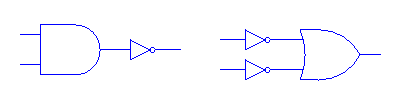
\includegraphics{figures/DeMorgan}}
}

\item Find the negation of each of the following and simplify as much as possible.
\medskip

  \begin{enumerate}
  \item $(A \lor B) \; \iff \; C$
\medskip

  \item $(A \lor B) \; \implies \; (A \land B)$

  \end{enumerate}

\wbvfill

\hint{Neither of these is particularly amenable to simplification. Nor, perhaps, is it readily
apparent what ``simplify'' means in this context! My interpretation is that we should look
for a logically equivalent expression using the fewest number of operators and if possible
{\em not} using the more complicated operators ($\implies$ and $\iff$).  However, if we try 
to rewrite the first statement's negation using only $\land$, $\lor$ and $\lnot$ we get things
that look a lot more complicated than $(A \lor B) \; \iff \; {\lnot}C$ -- the quick way to negate a 
bicondiitonal is simply to negate one of its parts.

The second statement's negation turns out to be the same thing as exclusive or, so a particularly
simple response would be to write $A \oplus B$ although that feels a bit like cheating, so
maybe we should answer with $(A \lor B) \land {\lnot}(A \land B)$ -- but that answer is what we
would get by simply applying the rule for negating a conditional and doing no further simplification.
}

\workbookpagebreak

\item Because a conditional sentence is equivalent to a certain disjunction, and 
because DeMorgan's law tells us that the negation of a disjunction is a conjunction,
it follows that the negation of a conditional is a conjunction.  Find denials (the negation
of a sentence is often called its ``denial'') for each of the following conditionals.

\begin{enumerate}
\item ``If you smoke, you'll get lung cancer.''
\item ``If a substance glitters, it is not necessarily gold.''
\item ``If there is smoke, there must also be fire.''
\item ``If a number is squared, the result is positive.''
\item ``If a matrix is square, it is invertible.''
\end{enumerate}

\wbvfill

\hint{
\begin{enumerate}
\item ``You smoke and you haven't got lung cancer.''
\item ``A substance glitters and it is necessarily gold.''
\item ``There is smoke,and there isn't fire.''
\item ``A number is squared, and the result is not positive.''
\item ``A matrix is square and it is not invertible.''
\end{enumerate}
}

\hintspagebreak
\workbookpagebreak

\item The so-called ``ethic of reciprocity'' is an idea that has come 
up in many of the world's religions and philosophies.  
Below are statements of the ethic
from several sources.  Discuss their logical meanings and determine which (if 
any) are logically equivalent.

\begin{enumerate}
\item ``One should not behave towards others in a way which is disagreeable to oneself.'' Mencius Vii.A.4 (Hinduism)
\item ``None of you [truly] believes until he wishes for his brother what he wishes for himself.'' Number 13 of Imam ``Al-Nawawi's Forty Hadiths.'' (Islam)
\item ``And as ye would that men should do to you, do ye also to them likewise.'' Luke 6:31, King James Version. (Christianity)
\item ``What is hateful to you, do not to your fellow man. This is the law: all the rest is commentary.'' Talmud, Shabbat 31a. (Judaism)
\item ``An it harm no one, do what thou wilt'' (Wicca)
\item ``What you would avoid suffering yourself, seek not to impose on others.'' (the Greek philosopher Epictetus -- first century A.D.)
\item ``Do not do unto others as you expect they should do unto you. Their tastes may not be the same.'' (the Irish playwright George Bernard Shaw -- 20th century A.D.)
\end{enumerate}

\wbvfill

\hint{
The ones from Wicca and George Bernard Shaw are just there for laughs.

For the remainder, you may want to contrast how restrictive they seem. For example the Christian version is (in my opinion) a lot stronger than the one from the Talmud -- ``treat others as you would want to be treated'' restricts your actions both in terms of what you would like done to you and in terms of what you wouldn't like done to you; ``Don't treat your fellows in a way that would be hateful to you.'' is leaving you a lot more freedom of action, since it only prohibits you from doing those things you wouldn't want done to yourself to others. The Hindus, Epictetus and the Jews (and the Wiccans for that matter) seem to be expressing roughly the same sentiment -- and promoting an ethic that is rather more easy for humans to conform to!

From a logical perspective it might be nice to define open sentences:

\[ W(x,y) \; = \; \mbox{``x would want y done to him.''} \]

\[ N(x,y)  \; = \; \mbox{``x would not want y done to him.''} \]

\[ D(x,y)  \; = \; \mbox{``do y to x.''} \]

\[ DD(x,y)  \; = \; \mbox{``don't do y to x.''} \]

In which case, the aphorism from Luke would be

\[ (W(you, y) \implies  D(others, y)) \land (N(you, y) \implies DD(others, y)) \]

}

\workbookpagebreak
\textbookpagebreak

\item You encounter two natives of the land of knights and knaves. Fill
in an explanation for each line of the proofs of their identities. 

\begin{enumerate}
\item Natasha says, ``Boris is a knave.'' \\
Boris says, ``Natasha and I are knights.''\\

\hintspagebreak

\textbf{Claim:} Natasha is a knight, and Boris is a knave.\\

\begin{proof} If Natasha is a knave, then Boris is a knight.\\
If Boris is a knight, then Natasha is a knight.\\
Therefore, if Natasha is a knave, then Natasha is a knight.\\
Hence Natasha is a knight.\\
Therefore, Boris is a knave.
\end{proof}

\item Bonaparte says ``I am a knight and Wellington is a knave.''\\
Wellington says ``I would tell you that B is a knight.''

\textbf{Claim:} Bonaparte is a knight and Wellington is a knave.

\begin{proof}
    Either Wellington is a knave or Wellington is a knight.\\
    If Wellington is a knight it follows that Bonaparte is a knight.\\
    If Bonaparte is a knight then Wellington is a knave. \\
    So, if Wellington is a knight then Wellington is a knave (which is impossible!)\\
    Thus, Wellington is a knave.\\
    Since Wellington is a knave, his statement ``I would tell you that Bonaparte is a knight'' is false. \\
    So Wellington would in fact tell us that Bonaparte is a knave. \\
    Since Wellington is a knave we conclude that Bonaparte is a knight.\\
    Thus Bonaparte is a knight and Wellington is a knave (as claimed).\\
\end{proof}

\hintspagebreak
\wbvfill

\hint{
Here's the second one:

\begin{proof}
    Either Wellington is a knave or Wellington is a knight.\\
    \rule{0pt}{0pt} \hfill \parbox{3in}{\color[rgb]{1,0,0} It's either one thing or the other! }\\
    If Wellington is a knight it follows that Bonaparte is a knight.\\
    \rule{0pt}{0pt} \hfill \parbox{3in}{\color[rgb]{1,0,0} That's what he said he would tell us and if he's a knight we can trust him.}\\
    If Bonaparte is a knight then Wellington is a knave. \\
    \rule{0pt}{0pt} \hfill \parbox{3in}{\color[rgb]{1,0,0} True, because that is one of the things Bonaparte states.}\\
    So, if Wellington is a knight then Wellington is a knave (which is impossible!)\\
    \rule{0pt}{0pt} \hfill \parbox{3in}{\color[rgb]{1,0,0} This is just summing up what was deduced above.}\\
    Thus, Wellington is a knave.\\
    \rule{0pt}{0pt} \hfill \parbox{3in}{\color[rgb]{1,0,0}  Because the other possibility leads to something {\em im}possible.}\\
    Since Wellington is a knave, his statement ``I would tell you that Bonaparte is a knight'' is false. \\
    \rule{0pt}{0pt} \hfill \parbox{3in}{\color[rgb]{1,0,0} Knave's statements are always false!}\\
    So Wellington would in fact tell us that Bonaparte is a knave. \\
    \rule{0pt}{0pt} \hfill \parbox{3in}{\color[rgb]{1,0,0} He was lying when he said he would tell us B is a knight.} \\
    Since Wellington is a knave we conclude that Bonaparte is a knight.\\
    \rule{0pt}{0pt} \hfill \parbox{3in}{\color[rgb]{1,0,0} Wait, now I'm confused\ldots can you do this part?} \\
    Thus Bonaparte is a knight and Wellington is a knave (as claimed).\\
    \rule{0pt}{0pt} \hfill \parbox{3in}{\color[rgb]{1,0,0} Just summarizing.} \\
\end{proof}

}

\end{enumerate}

\end{enumerate}


\newpage
\section{Two-column proofs}
\label{sec:2_col}

If you've ever spent much time trying to check someone else's work
in solving an algebraic problem, you'd probably agree that it 
would be a help to know what they were \emph{trying} to do in each
step.  Most people have this fairly vague notion that they're allowed 
to ``do the same thing on both sides'' and they're allowed to simplify
the sides of the equation separately -- but more often than not, several
different things get done on a given line, mistakes get made, and it can
be nearly impossible to figure out what went wrong and where.

Now, after all, the beauty of math is supposed to lie in its crystal clarity,
so this sort of situation is really unacceptable.  It may be an impossible
goal to get ``the average Joe'' to perform algebraic manipulations with
clarity, but those of us who aspire to become mathematicians must certainly
hold ourselves to a higher standard.  \index{two-column proof}Two-column proofs are usually what 
is meant by a ``higher standard'' when we are talking about relatively
mechanical manipulations -- like doing algebra, or more to the point,
proving logical equivalences.  Now don't despair!  You will not, in 
a mathematical career, be expected to provide two-column proofs very
often.  In fact, in more advanced work one tends to not give \emph{any} sort
of proof for a statement that lends itself to a two-column approach.  But,
if you find yourself writing ``As the reader can easily verify, Equation~17 holds\ldots'' in a paper, or making some similar remark to your students,
you are \emph{morally obligated} to being able to produce a two-column proof.

So what, exactly, is a two-column proof?  In the left column you show your 
work, being careful to go one step at a time.  In the right column you
provide a justification for each step. 

We're going to go through a couple of examples of two-column proofs 
in the context of proving logical equivalences.  One thing to watch out
for: if you're trying to prove a given equivalence, and the first thing 
you write down is that very equivalence, \emph{it's wrong!}  This 
would constitute the logical error known as 
\index{begging the question}``begging the question'' 
also known as \index{circular reasoning}``circular reasoning.''  
It's clearly not okay to try
to demonstrate some fact by first \emph{asserting the very same fact}.
Nevertheless, there is (for some unknown reason) a powerful temptation
to do this very thing.  To avoid making this error, we will not
put any equivalences on a single line.  Instead we will start with 
one side or the other of the statement to be proved, and modify it
using known rules of equivalence, until we arrive at the other side.

Without further ado, let's provide a proof of the equivalence  
$A \land (B \lor {\lnot}A) \; \cong \; A \land B $.\footnote{This equivalence should have been verified using truth tables in the exercises from the previous
section.}
\medskip

\begin{center}
\begin{tabular}{p{2in}p{2in}}
\rule{10pt}{0pt} $A \land (B \lor {\lnot}A)$ & \\
 & distributive law\\
$\cong (A \land B) \lor (A \land {\lnot}A)$ & \\
 & complementarity\\
$\cong (A \land B) \lor c$ & \\
 & identity law\\
$\cong (A \land B)$ & \\
\end{tabular}
\end{center}
\medskip

We have assembled a nice, step-by-step sequence of equivalences -- each
justified by a known law -- that begins with the left-hand side of the 
statement to be proved and ends with the right-hand side.  That's an 
irrefutable proof!

In the next example we'll highlight a slightly sloppy habit of thought
that tends to be problematic.  People usually (at first) associate a 
direction with the basic logical equivalences.  This is reasonable 
for several of them because one side is markedly simpler than the 
other.  For example, the domination rule would normally be used
to replace a part of a statement that looked like ``$A \land c$'' with
the simpler expression ``$c$''.  There is a certain amount of strategization
necessary in doing these proofs, and I usually advise people to start 
with the more complicated side of the equivalence to be proved.  It just
feels right to work in the direction of making things simpler, but there 
are times when one has to take one step back before proceeding two steps
forward\ldots   

Let's have a look at another equivalence: $A \land (B \lor C) \cong 
(A \land (B \lor C)) \lor (A \land C)$.  There are many different ways
in which valid steps can be concatenated to convert one side of this 
equivalence into the other, so a subsidiary goal is to find a proof that
uses the least number of steps.  Following my own advice, I'll start 
with the right-hand side of this one.
\medskip

\begin{center}
\begin{tabular}{p{2in}p{2in}}
\rule{10pt}{0pt} $(A \land (B \lor C)) \lor (A \land C)$ & \\
 & distributive law\\
$\cong  ((A \land B) \lor (A \land C)) \lor (A \land C)$ & \\
 & associative law\\
$\cong  (A \land B) \lor ((A \land C) \lor (A \land C))$ & \\
 & idempotence \\
$\cong (A \land B) \lor (A \land C) $ & \\
 & distributive law\\
$\cong A \land (B \lor C)$ & \\
\end{tabular}
\end{center}
\medskip

Note that in the example we've just done, the two applications
of the distributive law go in opposite directions as far as their
influence on the complexity of the expressions are concerned.

\clearpage

\noindent{\large \bf Exercises --- \thesection\ }


Write two-column proofs that verify each of the following
logical equivalences.

\begin{enumerate}
\item $A \lor (A \land B) \; \cong \; A \land (A \lor B)$
\medskip

\item $(A \land {\lnot}B) \lor A \; \cong \; A$
\medskip

\item $A \lor B \; \cong \; A \lor ({\lnot}A \land B)$
\medskip

\item ${\lnot}(A \lor {\lnot}B) \lor ({\lnot}A \land {\lnot}B) \; \cong \; {\lnot}A$
\medskip

\item $A \; \cong \; A \land ((A \lor {\lnot}B) \lor (A \lor B))$
\medskip

\item $(A \land {\lnot}B) \land ({\lnot}A \lor B) \; \cong \; c$
\medskip

\item $A \; \cong \; A \land (A \lor (A \land (B \lor C)))$
\medskip

\item ${\lnot}(A \land B) \land {\lnot}(A \land C) \; \cong \; {\lnot}A \lor ({\lnot}B \land {\lnot}C)$
\medskip

\end{enumerate}

\hint{
Here's the last one:

\begin{proof}

$  {\lnot}(A \land B) \land {\lnot}(A \land C) $ \\  
 \rule{0pt}{0pt} \hfill \parbox{3in}{\color[rgb]{1,0,0}  	 DeMorgan's law (times 2)} \\
$\equiv  \quad   ({\lnot}A \lor {\lnot}B) \land ({\lnot}A \lor {\lnot}C)	$ \\   
 \rule{0pt}{0pt} \hfill \parbox{3in}{\color[rgb]{1,0,0}  	 Distributive law} \\ 
$\equiv  \quad  {\lnot}A \lor ({\lnot}B \land {\lnot}C) $ \\  
\end{proof}

}
\workbookpagebreak

\rule{0pt}{0pt}

\workbookpagebreak


\newpage

\section{Quantified statements}
\label{sec:quant}

All of the statements discussed in the previous sections were of the 
``completely unambiguous'' sort; that is, they didn't have any {\em unknowns}  
in them.  As a reader of this text, it's a sure bet that you've mastered
Algebra and are firmly convinced of the utility of $x$ and $y$.  Admittedly,
we've used variables to refer to sentences (or sentence fragments) themselves,
but we've said that sentences that had variables {\em in them} were ambiguous 
and didn't even deserve to be called logical statements.  The notion 
of \index{quantification}{\em quantification} 
allows us to use the power of variables within a
sentence without introducing ambiguity.

Consider the sentence ``There are exactly 7 odd primes less than 20.''  
This sentence has some kind of ambiguity in it (because it doesn't mention
the primes explicitly) and yet it certainly seems to have a definite 
truth value!  The reason its truth value is known (by the way, it is T)
is that the sentence is quantified.  ``X is an odd prime less than 20.'' 
is an ambiguous sentence, but ``There are exactly 7 distinct X's that
are odd primes less than 20.'' is not.  This example represents a fairly
unusual form of quantification.  Usually, we take away the ambiguity
of a sentence having a variable in it by asserting one of two levels 
of quantification: ``this is true at least once'' or ``this is always true''.  
We've actually seen the symbols ($\exists$ and $\forall$) for these 
concepts already (in Section~\ref{sec:scary}).  

An \index{open sentence}{\em open sentence} 
is one that has variables in it.  We represent 
open sentences using a sort of functional notation to show what
variables are in them.  

Examples:

\begin{enumerate}

\item[i)] $P(x)$ = ``$2^{2^x}+1$ is a prime.''

\item[ii)] $Q(x,y)$ = ``$x$ is prime or $y$ is a divisor of $x$.''

\item[iii)] $L(f,c,l)$ = ``The function $f$ has limit $l$ at $c$, if 
and only if, 
for every positive number $\epsilon$, there is a positive number $\delta$ 
such that whenever $|x-c| < \delta$ it follows that $|f(x)-l| < \epsilon$.''  
\end{enumerate}

That last example certainly is a doozey!  At first glance it would appear
to have more than three variables in it, and indeed it does!  In order of
appearance, we have $f$, $l$, $c$, $\epsilon$, $\delta$ and $x$ -- the 
last three variables that appear ($\epsilon$, $\delta$ and $x$) are said
to be \index{bound variables}{\em bound}.  
A variable in an open sentence is bound if it is in the
scope of a quantifier.  Bound variables don't need to be mentioned
in the argument list of the sentence.  Unfortunately, when sentences are
given in natural languages the quantification status of a variable may 
not be clear.  For example in the third sentence above, the variable $\delta$
is easily seen to be in the scope of the quantifier $\exists$ because of the
words ``there is a positive number'' that precede it.  Similarly, $\epsilon$
is universally quantified ($\forall$) because the phrase ``for every positive
number'' appears before it.  What is the status of $x$?  Is it really bound?
The answers to such questions may not be clear at first, but after some 
thought you should be able to decide that $x$ is universally quantified.

\begin{exer} What word in example iii) indicates that $x$ is in the
scope of a $\forall$ quantifier?
\end{exer}

It is not uncommon, in advanced Mathematics, to encounter compound sentences
involving dozens of variables and 4 or 5 levels of quantification.  Such 
sentences seem hopelessly complicated at first sight -- the key to 
understanding them is to determine each variable's quantification status
explicitly and to break things down into simpler sub-parts.  

For instance, in understanding example iii) above, it might be
useful to define some new open sentences:

$D(x,c,\delta)$ = ``$|x-c| < \delta$''

$E(f,x,l,\epsilon)$ = ``$|f(x)-l| < \epsilon$''

\noindent Furthermore, it's often handy to replace an awkward phrase (such as 
``the limit of $f$ at $c$ is $l$'') with symbols when possible.
 
Example iii) now looks like 

\[ \lim_{x\rightarrow c}f(x) = l \iff \forall \epsilon>0 \, \exists \delta>0 \, \forall x \, D(x,c,\delta) \implies E(f,x,l,\epsilon). \]

The sentence $D(x,c,\delta)$ is usually interpreted as saying that
``$x$ is close to $c$'' (where $\delta$ tells you {\em how} close.)
The sentence $E(f,x,l,\epsilon)$ could be expressed informally as
``$f(x)$ is close to $l$'' (again, $\epsilon$ serves to make the 
word ``close'' more exact).

It's instructive to write this sentence one last time, {\em completely}
in symbols and without the abbreviations we created for saying
that $x$ is near $c$ and $f(x)$ is near $l$:


$\displaystyle \lim_{x\rightarrow c}f(x) = l \iff \forall \epsilon>0 \, \exists 
\delta>0 \, \forall x \, (|x-c| < \delta) \implies (|f(x)-l| < \epsilon) $.

It would not be unfair to say that developing the facility to read,
and understand, this hieroglyph (and others like it) constitutes the 
first several weeks of a course in Real Analysis.

Let us turn back to another of the examples (of an open sentence) from the
beginning of this section.  $P(x)$ = ``$2^{2^x}+1$ is a prime.''

In the 17th century, \index{Fermat, Pierre de}Pierre de Fermat 
made the conjecture\footnote{Fermat's 
more famous conjecture, that $x^n+y^n=z^n$ has no non-trivial integer solutions
if $n$ is an integer with $n>2$ was discovered after his death.} that 
$\forall x \in {\mathbb N}, P(x)$.  No doubt, this seemed reasonable to Fermat
because the numbers given by this formula (they are called 
\index{Fermat numbers}Fermat numbers in
his honor) are all primes -- at first!  Fermat numbers are conventionally
denoted with a subscripted letter F,  $F_n = 2^{2^n}+1$, the first five
Fermat numbers are prime.

\begin{center}
$\displaystyle F_0 = 2^{2^0}+1 = 3$\\
$\displaystyle F_1 = 2^{2^1}+1 = 5$\\
$\displaystyle F_2 = 2^{2^2}+1 = 17$\\
$\displaystyle F_3 = 2^{2^3}+1 = 257$\\
$\displaystyle F_4 = 2^{2^4}+1 = 65537$\\
\end{center}
 
Fermat probably computed that $F_5=4294967297$, and we can well imagine
that he checked that this number was not divisible by any small primes. 
Of course, this was well before the development of effective computing
machinery, so we shouldn't blame Fermat for not noticing that
$4294967297 = 641 \cdot 6700417$.  This remarkable feat of factoring 
can be replicated in seconds on a modern computer, however it was done
first by \index{Euler, Leonhard} Leonhard Euler in 1732!  
There is quite a lot of literature 
concerning the primeness and/or compositeness of Fermat numbers.  So
far, all the Fermat numbers between $F_5$ and $F_{32}$ (inclusive) have
been shown to be composite.  One might be tempted to conjecture that
only the first five Fermat numbers are prime, however this temptation
should be resisted \ldots  

Let us set aside, for the moment, further questions about Fermat numbers.
Suppose we define the set $U$ (for `Universe') by $U=\{0,1,2,3,4\}$.
Then the assertion, ``$\forall x \in U, P(x)$.'' is certainly true.
You should note that the only variable in this sentence is $x$, and
that the variable is bound -- it is universally quantified.  Open sentences
that have all variables bound are {\em statements}.  It is possible 
(in principle, and in finite universes, in practice) to check the 
truth value of such sentences.
Indeed, the sentence ``$\forall x \in U, P(x)$'' has the same logical content
as ``$P(0) \land P(1) \land P(2) \land P(3)  \land P(4)$''.  Both happen to be
true, but the real point here is to note that a universally quantified sentence
can be thought of instead as a conjunction.

\begin{exer}
Define a new set $U$ by $U=\{0,1,2,3,4,5\}$.  
Write a sentence using disjunctions
that is equivalent to ``$\exists x \in U, {\lnot}P(x)$.''
\end{exer}

Even when we are dealing with infinite universes, it is possible to
think of universally quantified sentences in terms of conjunctions,
and existentially quantified sentences in terms of disjunctions.  For
example, a quick look at the graphs should be sufficient to convince you
that ``$ x > \ln x $'' is a sentence that is true for all $x$ values in
${\mathbb R}^+$.  There is a notation, reminiscent of so-called sigma notation
for sums, that can be used to express this universally quantified sentence as
a conjunction.

\[
\forall x \in {\mathbb R}^+, x > \ln x \; \cong \; 
\bigwedge_{x \in {\mathbb R}^+} x > \ln x
\]

A similar notation exists for disjunctions.  Purely as an example, consider
the following problem from recreational math: Find a four digit number that
is an integer multiple of its reversal.  (By reversal, we mean the four
digit number with the digits in the opposite order -- for example, the
reversal of 1234 is 4321.)  The sentence\footnote{This sentence uses what %
is commonly referred to as an ``abuse of notation'' in order avoid an %
unnecessarily complex problem statement.  One should not necessarily %
avoid such abuses if one's readers can be expected to easily understand %
what is meant, any more than one should completely eschew the splitting %
of infinitives.}
that states that this question has a solution is

\[
\exists abcd \in {\mathbb Z},  \exists k \in {\mathbb Z}, abcd = k\cdot dcba
\]

This could be expressed instead as the disjunction of 9000 statements, or more 
compactly as

\[
\bigvee_{1000\leq abcd \leq 9999}  \exists k \in {\mathbb Z}, abcd = k\cdot dcba.
\]

\begin{exer} The existential statement above is true because $8712 = 4\cdot 2178$.
There is one other solution -- find it!
\end{exer}

An important, or at least useful, talent for a Mathematics student to develop
is the ability to negate quantified sentences.  The major reason for this
is the fact that the contrapositive of a conditional sentence is logically
equivalent to it.  This leads to a method known as 
\index{proof by contraposition}``proof by contraposition''
which can be expressed succinctly by the advice:

``If you get stuck, try writing down the contrapositive.''

Since writing down the contrapositive will often involve finding the
negation of a quantified sentence, let's try a few.

Our universe of discourse\footnote{The Pep Boys -- Manny, Moe and %
Jack -- are hopefully known to some readers as the mascots of a chain %
of automotive supply stores.} 
will be $P = \{ \mbox{Manny}, \mbox{Moe}, \mbox{Jack} \}$.  
Consider the sentence 
``$\forall x \in P, x\; \mbox{starts with M}$.''   The equivalent sentence
expressed conjunctively is 

\begin{gather*} (\mbox{Manny starts with M}) \land \\
(\mbox{Moe starts with M}) \land \\
(\mbox{Jack starts with M}).
\end{gather*}

\noindent  The negation
of this sentence (by DeMorgan's law) is a disjunction:

\begin{gather*}
(\mbox{Manny doesn't start with M}) \lor \\ 
(\mbox{Moe doesn't start with M}) \lor \\
(\mbox{Jack doesn't start with M})
\end{gather*}

\noindent Finally, this disjunction of three sentences can be converted into 
a single sentence, existentially quantified over $P$:

``$\exists x \in P, {\lnot}(x \, \mbox{starts with M})$.'' 

The discussion in the previous paragraphs justifies some laws of 
Logic which should be thought of as generalizations of DeMorgan's laws:

\[ 
{\lnot}( \forall x \in U, P(x)) \; \cong \; \exists x \in U, {\lnot}P(x)
\]

\noindent and

\[ 
{\lnot}( \exists x \in U, P(x)) \; \cong \; \forall x \in U, {\lnot}P(x).
\]

It's equally valid to think of these rules in a way that's divorced from
DeMorgan's laws.  To show that a universal sentence is {\em false}, it suffices
to show that an existential sentence involving a negation of the original is 
true.\footnote{To show that it is not the case that every Pep boy's name starts
with `M', one only needs to demonstrate that there is a Pep boy (Jack) whose 
name doesn't start with `M'.}

\clearpage

\noindent{\large \bf Exercises --- \thesection\ }

\begin{enumerate}
\item There is a common variant of the existential quantifier,
$\exists !$, if you write $\exists ! \, x, \, P(x)$ you are asserting 
that there is a \index{unique existence}\emph{unique} element 
in the universe that makes $P(x)$ true.
Determine how to negate the sentence $\exists ! \, x, \, P(x)$.

\hint{
Unique existence is essentially saying that there is exactly 1 element of the universe of discourse that makes P(x) true. The negation of "there is exactly 1" is "there's either none, or at least 2".

Is that enough of a hint?
}

\item The order in which quantifiers appear is important.  Let $L(x,y)$
be the open sentence ``$x$ is in love with $y$.''  Discuss the meanings of the
following quantified statements and find their negations.

\begin{enumerate}
\item $\forall x \, \exists y \; L(x,y)$.
\item $\exists x \, \forall y \; L(x, y)$.
\item $\forall x \, \forall y \; L(x, y)$.
\item $\exists x \, \exists y \; L(x, y)$.
\end{enumerate}

\hint{

\begin{enumerate}
\item $\forall x \, \exists y \; L(x,y)$.

This is a fairly optimistic statement  ``For everyone out there, there's somebody that they are in love with.''

\item $\exists x \, \forall y \; L(x, y)$.

This one, on the other hand, says something fairly strange: ``There's someone who has fallen in love with every other human being.'' I don't know, maybe the Dalai Lama? Mother Theresa?...
Anyway, do the last two for yourself.

\item $\forall x \, \forall y \; L(x, y)$.
\item $\exists x \, \exists y \; L(x, y)$.

\vspace{.5in}

Here's a couple of bonus questions. Two of the statements above have different meanings if you just interchange the order that the quantifiers appear in. What do the following mean (in contrast to the ones above)?

\item $\exists y \, \forall x \; L(x, y)$.
\item $\forall y \, \exists x \; L(x,y)$.
\end{enumerate}

}

\item Determine a useful denial of: 

$\displaystyle \forall \epsilon>0 \, \exists 
\delta>0 \, \forall x \, (|x-c| < \delta) \implies (|f(x)-l| < \epsilon) $.

The denial above gives a criterion for saying $\lim_{x\rightarrow c}f(x) \neq l.$

\hint{
This is asking you to put a couple of things together. The first thing is that in negating a quantified statement, we get a new statement with all the quantified variables occurring in the same order but with $\forall$'s and $\exists$'s interchanged. The second issue is that the logical statement that appears after all the quantifiers needs to be negated. Since, in this statement we have a conditional, you must remember to negate that properly (its negation is a conjunction).

$\displaystyle \exists \epsilon>0 \, \forall 
\delta>0 \, \exists x \, (|x-c| < \delta)  \land  (|f(x)-l| \geq \epsilon) $.

}

\item A \index{Sophie Germain prime} \emph{Sophie Germain prime} is a prime number $p$
such that the corresponding odd number $2p+1$ is also a prime.  For example 11 is a 
Sophie Germain prime since $23 = 2\cdot 11 + 1$ is also prime.  Almost all Sophie Germain
primes are congruent to $5 \pmod{6}$, nevertheless, there are exceptions -- so the
statement ``There are Sophie Germain primes that are not 5 mod 6.'' is true.  Verify this.

\hint{The exceptions are very small prime numbers. You should be able to find them easily.}

\item  Alvin, Betty, and Charlie enter a cafeteria which offers three different
entrees, turkey sandwich, veggie burger, and pizza; four different
beverages, soda, water, coffee, and milk; and two types of desserts,
pie and pudding. Alvin takes a turkey sandwich, a soda, and a pie.
Betty takes a veggie burger, a soda, and a pie. Charlie takes a pizza
and a soda. Based on this information, determine whether the following
statements are true or false.

\begin{enumerate}
\item \label{negated}$\forall$ people $p$, $\exists$ dessert $d$ such that $ p$
took $d$. \hint{false}
\item \label{compare}$\exists$ person $p$ such that $\forall$ desserts
$d$, $p$ did not take $d$. \hint{true}
\item $\forall$ entrees $e$, $\exists$ person $p$ such that $ p$ took
$e$. \hint{true}
\item \label{entree}$\exists$ entree $e$ such that  $\forall$ people
$p,\ p$ took $e$. \hint{false}
\item $\forall$ people $p$, $p$ took a dessert $\iff p$ did not take
a pizza. \hint{true}
\item Change one word of statement \ref{entree} so that it becomes true. \hint{entree $\longrightarrow$ beverage}
\item Write down the negation of \ref{negated} and compare it to statement
\ref{compare}. Hopefully you will see that they are the same! Does
this make you want to modify one or both of your answers to \ref{negated}
and \ref{compare}? \hint{$\exists$ person $p$ such that $\forall$ desserts
$d$, $p$ did not take $d$. Yes I do.  No, I got them right in the first place!}
\end{enumerate}

\end{enumerate}



\newpage

\section{Deductive reasoning and Argument forms}
\label{sec:deduct}

Deduction \index{deduction}
is the process by which we determine new truths from old.  
It is sometimes claimed that nothing truly new can come from deduction, 
the truth of a statement that is arrived at by deductive processes was 
lying (perhaps hidden somewhat) within the hypotheses.  This claim is something
of a canard, as any Sherlock Holmes aficionado can tell you, the statements
that can sometimes be deduced from others can be remarkably surprising.  
A better
argument against deduction is that it is a relatively ineffective way for most 
human beings to discover new truths -- for that purpose inductive processes are
superior for the majority of us.  Nevertheless, if a chain of deductive reasoning
leading from known hypotheses to a particular conclusion can be exhibited, the truth
of the conclusion is \emph{unassailable}.  For this reason, mathematicians have 
latched on to deductive reasoning as \emph{the} tool for, if not discovering 
our theorems, communicating them to others.  

The word ``argument'' has a negative connotation for many people because 
it seems to have to do with {\em disagreement}.  Arguments within mathematics
(as well as many other scholarly areas), while they may be impassioned, should
not involve discord.  A mathematical argument is a sequence of logically
connected statements designed to produce {\em agreement} as to the validity
of a proposition.  This ``design'' generally follows one of two possibilities,
inductive reasoning or deductive reasoning.  In an inductive argument 
a long list of premises is presented whose truths are considered to be
apparent to all, each of which provides evidence that the desired conclusion
is true.  So an \index{inductive argument}inductive argument represents a kind of statistical thing,
you have all these statements that are true each of which indicates that 
the conclusion is most likely true\ldots  A strong inductive argument
amounts to what attorneys call a ``preponderance of the evidence.''  
Occasionally
a person who has been convicted of a crime based on a preponderance of the 
evidence is later found to be innocent.  This usually happens when new evidence
is discovered that incontrovertibly proves (i.e. shows through deductive
means) that he or she cannot be guilty.  In a nutshell: inductive arguments
can be wrong. 

In contrast a deductive argument can only turn out to be wrong under 
certain well-understood circumstances.

Like an inductive argument, a \index{deductive argument}deductive argument 
is essentially just a
long sequence of statements; but there is some additional structure.
The last statement in the list is the {\em conclusion} -- the statement
to be proved -- those occurring before it are known as 
\index{premise}{\em premises}.
Premises may be further subdivided into (at least) five sorts: axioms,
definitions, previously proved theorems, hypotheses and deductions.  
Axioms and definitions are often glossed
over, indeed, they often go completely unmentioned (but rarely {\em unused}) 
in a proof.  In the interest of brevity this is quite appropriate, but 
conceptually, you should think of an argument as being based off of 
the axioms for the particular area you are working in, and its standard 
definitions.  A rote knowledge of all the other theorems proved up to
the one you are working with would generally be considered excessive, 
but completely memorizing the axioms and standard definitions of a field 
is essential.  \index{hypotheses}Hypotheses are a funny class of premises -- they are things
which can be assumed true for the sake of the current argument.  For
example, if the statement you are trying to prove is a conditional,
then the antecedent may be assumed true (if the antecedent is false,
then the conditional is automatically true!).  You should always be
careful to list all hypotheses explicitly, and at the end of your 
proof make sure that each and every hypothesis got used somewhere 
along the way.  If a hypothesis really isn't necessary then you have
proved a more general statement (that's a good thing). 

Finally, deductions -- I should note that the conclusion is also a 
deduction -- obey a very strict rule: every deduction follows from
the premises that have already been written down (this includes
axioms and definitions that probably won't actually have been written,
hypotheses and all the deductions made up to this point) by one of the 
so-called \index{rules of inference}rules of inference.

Each of the rules of inference actually amounts to a logical tautology
that has been re-expressed as a sort of re-writing rule.   Each rule
of inference will be expressed as a list of logical 
sentences that are assumed to be among the premises of the argument, 
a horizontal bar, followed by the symbol $\therefore$ (which is
usually voiced as the word ``therefore'') and then a new statement 
that can be placed among the deductions.

For example, one (very obvious) rule of inference is

\begin{center}
\begin{tabular}{cl}
 & $A \land B$ \\ \hline
$\therefore$ & $B$\\
\end{tabular}
\end{center}
  
\noindent This rule is known as 
\index{conjunctive simplification}\emph{conjunctive simplification}, and
is equivalent to the tautology $(A \land B) \implies B$. 

The \index{modus ponens}\emph{modus ponens} 
rule\footnote{Latin for ``method of affirming'',
the related \emph{modus tollens} rule means ``method of denying.''} 
is one of the most useful.

\begin{center}
\begin{tabular}{cl}
 & $A$ \\
 & $A \implies B$ \\ \hline
$\therefore$ & $B$ \\
\end{tabular}
\end{center}

Modus ponens is related to the tautology $(A \land (A \implies B)) \implies B$.

\index{modus tollens}\emph{Modus tollens} 
is the rule of inference we get if we put modus ponens 
through the ``contrapositive'' wringer.

\begin{center}
\begin{tabular}{cl}
 & ${\lnot}B$ \\
 & $A \implies B$ \\ \hline
$\therefore$ & ${\lnot}A$ \\
\end{tabular}
\end{center}

Modus tollens is related to the tautology $({\lnot}B \land (A \implies B)) \implies {\lnot}A$.

Modus ponens and modus tollens are also known as 
\index{syllogism}\emph{syllogisms}.  A 
syllogism is an argument form wherein a deduction follows from two premises.
There are two other common syllogisms, 
\index{hypothetical syllogism}\emph{hypothetical syllogism} and
\index{disjunctive syllogism}\emph{disjunctive syllogism}.

Hypothetical syllogism basically asserts a transitivity property for 
implications.

\begin{center}
\begin{tabular}{cl}
 & $A \implies B$ \\
 & $B \implies C$ \\ \hline
$\therefore$ & $A \implies C$ \\
\end{tabular}
\end{center}

Disjunctive syllogism can be thought of as a statement about
alternatives, but be careful to remember that in Logic, the disjunction
always has the inclusive sense.

\begin{center}
\begin{tabular}{cl}
 & $A \lor B$ \\
 & ${\lnot}B$ \\ \hline
$\therefore$ & $A$ \\
\end{tabular}
\end{center}

\begin{exer}
Convert the $A \lor B$ that appears in the premises of the disjunctive
syllogism rule into an equivalent conditional.  How is the new argument
form related to modus ponens and/or modus tollens?
\end{exer}
 
The word ``dilemma'' usually refers to a situation in which an individual
is faced with an impossible choice.  A cute example known as the 
\index{Crocodile's dilemma}Crocodile's dilemma is as follows:

\begin{quote}
A crocodile captures a little boy who has strayed too near the river.  The 
child's father appears and the crocodile tells him ``Don't worry, I shall 
either release your son or I shall eat him.  If you can say, in advance,
which I will do, then I shall release him.''  The father responds, ``You will
eat my son.''  What should the crocodile do?
\end{quote} 

In logical arguments the word dilemma is used in another sense having to
do with certain rules of inference.  
\index{constructive dilemma}\emph{Constructive dilemma} is 
a rule of inference having to do with the conclusion that one of two 
possibilities must hold.

\begin{center}
\begin{tabular}{cl}
 & $A \implies B$ \\
 & $C \implies D$ \\ 
 & $A \lor C$ \\ \hline
$\therefore$ & $B \lor D$ \\
\end{tabular}
\end{center}

\index{destructive dilemma}\emph{Destructive dilemma} 
is often not listed among the rules
of inference because it can easily be obtained by using the constructive
dilemma and replacing the implications with their contrapositives.

\begin{center}
\begin{tabular}{cl}
 & $A \implies B$ \\
 & $C \implies D$ \\ 
 & ${\lnot}B \lor {\lnot}D$ \\ \hline
$\therefore$ & ${\lnot}A \lor {\lnot}C$ \\
\end{tabular}
\end{center}

In Table~\ref{tab:roi}, the ten most common 
\index{rules of inference}rules of inference are listed.  
Note that all of these are equivalent to tautologies that
involve conditionals (as opposed to biconditionals), every one of the 
basic logical equivalences that we established in Section~\ref{sec:le}
is really a tautology involving a biconditional, collectively these are
known as the \index{rules of replacement}``rules of replacement.''  
In an argument, any statement
allows us to infer a logically equivalent statement.  Or, put differently,
we could replace any premise with a different, but logically equivalent,
premise.  You might enjoy trying to determine a minimal set of rules of
inference, that together with the rules of replacement would allow one
to form all of the same arguments as the ten rules in Table~\ref{tab:roi}.
  
\begin{table}[hbt] 
\begin{center}
\begin{tabular}{c|c}
Name & Form \\ \hline
 & \\
Modus ponens \rule{12pt}{0pt} &   
\rule{24pt}{0pt}\begin{tabular}{cl}
 & $A$ \\
 & $A \implies B$ \\ \hline
$\therefore$ & $B$ \\
\end{tabular} \\
 & \\ \hline
 & \\
Modus tollens \rule{12pt}{0pt} &
\rule{24pt}{0pt}\begin{tabular}{cl}
 & ${\lnot}B$ \\
 & $A \implies B$ \\ \hline
$\therefore$ & ${\lnot}A$ \\
\end{tabular}  \\ 
 & \\ \hline
 & \\
Hypothetical syllogism \rule{12pt}{0pt} &
\rule{24pt}{0pt}\begin{tabular}{cl}
 & $A \implies B$ \\
 & $B \implies C$ \\ \hline
$\therefore$ & $A \implies C$ \\
\end{tabular} \\ 
 & \\ \hline 
 & \\
Disjunctive syllogism \rule{12pt}{0pt} &
\rule{24pt}{0pt}\begin{tabular}{cl}
 & $A \lor B$ \\
 & ${\lnot}B$ \\ \hline
$\therefore$ & $A$ \\
\end{tabular}  \\ 
 & \\ \hline 
 & \\
Constructive dilemma \rule{12pt}{0pt} & 
\rule{24pt}{0pt} \begin{tabular}{cl}
 & $A \implies B$ \\
 & $C \implies D$ \\ 
 & $A \lor C$ \\ \hline
$\therefore$ & $B \lor D$ \\
\end{tabular} \\
 & \\ 
\end{tabular}
\end{center}
\caption{The rules of inference.}
\label{tab:roi}
\end{table}
\clearpage

\rule{0pt}{0pt}

\vspace{.4in}

\begin{center}
\begin{tabular}{c|c}
Name & Form \\ \hline
 & \\
Destructive dilemma \rule{12pt}{0pt} & 
\rule{24pt}{0pt}\begin{tabular}{cl}
 & $A \implies B$ \\
 & $C \implies D$ \\ 
 & ${\lnot}B \lor {\lnot}D$ \\ \hline
$\therefore$ & ${\lnot}A \lor {\lnot}C$ \\
\end{tabular} \\ 
 & \\ \hline
 & \\
Conjunctive simplification \rule{12pt}{0pt} &
\rule{24pt}{0pt}\begin{tabular}{cl}
 & $A \land B$ \\ \hline
$\therefore$ & $A$ \\
\end{tabular} \\ 
 & \\ \hline
 & \\
Conjunctive addition \rule{12pt}{0pt} &
\rule{24pt}{0pt}\begin{tabular}{cl}
 & $A$ \\
 & $B$ \\ \hline
$\therefore$ & $A \land B$ \\
\end{tabular}  \\ 
 & \\ \hline
 & \\
Disjunctive addition \rule{12pt}{0pt} &
\rule{24pt}{0pt}\begin{tabular}{cl}
 & $A$ \\ \hline
$\therefore$ & $A \lor B$ \\
\end{tabular} \\ 
 & \\ \hline
 & \\
Absorption \rule{12pt}{0pt} &
\rule{24pt}{0pt}\begin{tabular}{cl}
 & $A \implies B$ \\ \hline
$\therefore$ & $A \implies (A \land B)$ \\
\end{tabular}  \\ 
 & \\
\end{tabular}

\vspace{.25in}

Table~\ref{tab:roi}: The rules of inference. (continued)
\index{rules of inference}
\end{center}


\newpage

\noindent{\large \bf Exercises --- \thesection\ }

\begin{enumerate}

\item In the movie ``Monty Python and the Holy Grail'' we encounter
a medieval villager who (with a bit of prompting) makes the 
following argument.

\begin{quote}
If she weighs the same as a duck, then she's made of wood. \newline
If she's made of wood then she's a witch. \newline
Therefore, if she weighs the same as a duck, she's a witch.
\end{quote} 

Which rule of inference is he using?

\hint{
This is what many people refer to as the transitive rule of implication.  As an argument form it's known as ``hypothetical syllogism.''
}

\item In constructive dilemma, the antecedent of the conditional 
sentences are usually chosen to represent opposite alternatives. 
This allows us to introduce their disjunction as a tautology. 
Consider the following proof that there is never any reason to worry
(found on the walls of an Irish pub).

\begin{quote}
Either you are sick or you are well. \newline
If you are well there's nothing to worry about. \newline
If you are sick there are just two possibilities: \newline
Either you will get better or you will die. \newline
If you are going to get better there's nothing to worry about. \newline
If you are going to die there are just two possibilities:\newline
Either you will go to Heaven or to Hell. \newline
If you go to Heaven there is nothing to worry about.
If you go to Hell, you'll be so busy shaking hands with all your friends there won't be time to worry \ldots
\end{quote}

Identify the three tautologies that are introduced in this ``proof.''

\hint{Look at the lines that start with the word "Either."}

\textbookpagebreak

\item For each of the following arguments, write it in symbolic form and determine 
which rules of inference are used.

\begin{enumerate}
\item \rule{0pt}{24pt} You are either with us, or you're against us.  And you don't appear to be with us.
So, that means you're against us!

\hint{
\begin{center}
\begin{tabular}{cl}
 & $W \lor A$ \\
 & ${\lnot}W$ \\ \hline
$\therefore$ & $A$ \\
\end{tabular}
\end{center}

This is ``disjunctive syllogism.''
}


\item \rule{0pt}{24pt} All those who had cars escaped the flooding.  Sandra had a car -- therefore, Sandra
escaped the flooding.

\hint{
Let $C(x)$ be the open sentence ``x has a car'' and let $E(x)$ be the open sentence ``x escaped the flooding.''
This argument is actually the particular form of universal modus ponens: (See the final question in the next set of exercises.)

\begin{center}
\begin{tabular}{cl}
 & $\forall x, C(x) \implies E(x)$ \\
 & $C(\mbox{Sandra}) $ \\ \hline
$\therefore$ & $E(\mbox{Sandra})$ \\
\end{tabular}
\end{center}

At this stage in the game it would be perfectly fine to just identify this as modus ponens and not worry about the quantifiers that appear.
}

\item \rule{0pt}{24pt}  When Johnny goes to the casino, he always gambles 'til he goes broke.  Today, Johnny
has money, so Johnny hasn't been to the casino recently.
\item \rule{0pt}{24pt} (A non-constructive proof that there are 
irrational numbers $a$ and $b$ such that $a^b$ is rational.)  
Either $\sqrt{2}^{\sqrt{2}}$ is rational or it is irrational.
If $\sqrt{2}^{\sqrt{2}}$ is rational, we let $a=b=\sqrt{2}$.
Otherwise, we let $a=\sqrt{2}^{\sqrt{2}}$ and $b=\sqrt{2}$.
(Since $\sqrt{2}^{\sqrt{2}^{\sqrt{2}}} = 2$, which is rational.) It follows that in either case, there
are irrational numbers $a$ and $b$ such that $a^b$ is rational.


\end{enumerate}

\hint{I'm leaving the last two for you to do. One small hint: both are valid forms.}


\end{enumerate}


\newpage

\section{Validity of arguments and common errors}
\label{sec:valid}

An argument is said to be \emph{valid} or to have a 
\index{valid argument form}\emph{valid form} 
if each deduction in it can be justified with one of the rules
of inference listed in the previous section.  The \emph{form} of 
an argument might be valid, but still the conclusion may be false
if some of the premises are false.  So to show that an argument is
good we have to be able to do two things: show that the argument 
is \emph{valid} (i.e. that every step can be justified) and that 
the argument is 
\index{soundness (of an argument)}\emph{sound} 
which means that all the premises are
true.  If you start off with a false premise, you can prove \emph{anything}!

Consider, for example the following ``proof'' that $2=1$.

\begin{quote}
  Suppose that $a$ and $b$ are two real numbers such that $a=b$.

\begin{center}
\begin{tabular}{p{2in}p{2in}}
 & by hypothesis, $a$ and $b$ are equal, so\\
 $a^2 = ab$ & \\
 & subtracting $b^2$ from both sides\\
 $a^2 - b^2 = ab - b^2$& \\
 & factoring both sides\\
 $(a+b)(a-b) = b(a-b)$ & \\
 & canceling $(a-b)$ from both sides\\
 $a+b = b$ & \\
\end{tabular}
\end{center}
\medskip
Now let $a$ and $b$ both have a particular value, $a=b=1$,
and we see that $1+1=1$, i.e. $2=1$.
\end{quote}

This argument is not sound (thank goodness!) because one of the
premises -- actually the bad premise appears as one of the 
justifications of a step -- is false.  You can argue with
perfect logic to achieve complete nonsense if you include 
false premises.

\begin{exer}
It is \emph{not} true that you can always cancel the same thing from 
both sides of an equation.  Under what circumstances is such cancellation
disallowed?
\end{exer}

So, how can you tell if an argument has a valid form?  Use a truth table.
As an example, we'll verify that the rule of inference known as 
\index{destructive dilemma}``destructive dilemma'' 
is valid using a truth table.  This argument
form contains 4 predicate variables so the truth table will have 16 rows.
There is a column for each of the variables, the premises of the argument
and its conclusion.

\begin{center}
\begin{tabular}{cccc|c|c|c|c|}
$A$   & $B$   & $C$   & $D$   & $A{\implies}B$ & $C{\implies}D$ & ${\lnot}B \lor {\lnot}D$ & ${\lnot}A \lor {\lnot}C$ \\ \hline
T     & T     & T     & T     & T     & T     & $\phi$ & $\phi$ \\
T     & T     & T     & $\phi$ & T     & $\phi$ & T     & $\phi$ \\
T     & T     & $\phi$ & T     & T     & T     & $\phi$ & T     \\
T     & T     & $\phi$ & $\phi$ & T     & T     & T     & T     \\
T     & $\phi$ & T     & T     & $\phi$ & T     & T     & $\phi$ \\
T     & $\phi$ & T     & $\phi$ & $\phi$ & $\phi$ & T     & $\phi$ \\
T     & $\phi$ & $\phi$ & T     & $\phi$ & T     & T     & T     \\
T     & $\phi$ & $\phi$ & $\phi$ & $\phi$ & T     & T     & T     \\ 
$\phi$ & T     & T     & T     & T     & T     & $\phi$ & T     \\
$\phi$ & T     & T     & $\phi$ & T     & $\phi$ & T     & T     \\
$\phi$ & T     & $\phi$ & T     & T     & T     & $\phi$ & T     \\
$\phi$ & T     & $\phi$ & $\phi$ & T     & T     & T     & T     \\
$\phi$ & $\phi$ & T     & T     & T     & T     & T     & T     \\
$\phi$ & $\phi$ & T     & $\phi$ & T     & $\phi$ & T     & T     \\
$\phi$ & $\phi$ & $\phi$ & T     & T     & T     & T     & T     \\
$\phi$ & $\phi$ & $\phi$ & $\phi$ & T     & T     & T     & T     \\
\end{tabular}
\end{center}

Now, mark the lines in which all of the premises of this argument form 
are true.  You should note that {\em in every single situation in which 
all the premises are true} the conclusion is also true.  That's what 
makes ``destructive dilemma'' -- and all of its friends -- a rule of 
inference.  Whenever all the premises are true so is the conclusion.  
You should also notice that there are several rows in which the 
conclusion is true but some one of the premises isn't.  That's
okay too, isn't it reasonable that the conclusion of an argument 
can be true, but at the same time the particulars of the argument 
are unconvincing? 

As we've noted earlier, an argument by deductive reasoning can go wrong 
in only certain well-understood ways.  Basically, either the form of the 
argument is invalid, or at least one of the premises is false.  Avoiding 
false premises in your arguments can be trickier than it sounds -- many 
statements that sound appealing or intuitively clear are actually
counter-factual.  The other side of the coin, being sure that the 
\index{form (of an argument)}\emph{form} 
of your argument is valid, seems easy enough -- just be 
sure to only use the rules of inference as found in Table~\ref{tab:roi}.  
Unfortunately most arguments that you either read or write
will be in prose, rather than appearing as a formal list of deductions.  
When dealing with that setting -- using natural rather than formalized 
language -- making errors in form is quite common.  

Two invalid forms are usually singled out for criticism, the 
\index{converse error}\emph{converse error} and the 
\index{inverse error}\emph{inverse error}.  In some sense 
these two apparently different ways to screw up are really the same thing.  
Just as a conditional statement and its contrapositive are known to be 
equivalent, so too are the other related statements -- the
converse and the inverse -- equivalent.  The converse error consists of 
mistaking the implication in a modus ponens form for its converse.

The converse error:

\begin{center}
\begin{tabular}{cl}
 & $B$ \\
 & $A \implies B$ \\ \hline
$\therefore$ & $A$ \\
\end{tabular}
\end{center}
   
Consider, for a moment the following argument.

\begin{quote}
If a rhinoceros sees something on fire, it will stomp on it. \newline
A rhinoceros stomped on my duck. \newline
Therefore, the rhino must have thought that my duck was on fire.
\index{duck, flaming}
\end{quote} 

It \emph{is} true that rhinoceroses have an instinctive desire to extinguish 
fires.  Also, we can well imagine that if someone made this ridiculous 
argument that their duck must actually have been crushed by a rhino.  But, 
is the conclusion that the duck was on fire justified?  Not really, what 
the first part of the argument asserts is that ``(on fire) implies (rhino 
stomping)'' but couldn't a rhino stomp on something for other reasons?  
Perhaps the rhino was just ill-tempered.  Perhaps the duck was just 
horrifically unlucky.

The closer the conditional is to being a biconditional, the more reasonable 
sounding is an argument exhibiting the converse error.  Indeed, if the 
argument actually contains a biconditional, the ``converse error'' is not 
an error at all.

The following is a perfectly valid argument, that (sadly) has a false premise.

\begin{quote}
You will get an A in your Foundations class if and only if you 
read Dr.\ Fields' book.\newline
You read Dr.\ Fields' book. \newline
Therefore, you will get an A in Foundations.
\end{quote}

Suppose that we try changing the major premise of that last argument to
something more believable.

\begin{quote}
If you read Dr.\ Fields' book, you will pass your Foundations class. \newline
You did not read Dr.\ Fields' book. \newline
Therefore, you will not pass Foundations.
\end{quote}

This last argument exhibits the so-called \emph{inverse error}.  It is by 
no means meant as a guarantee, but nevertheless, it seems reasonable that 
if someone reads this book they will pass a course on this material.  
The second premise is also easy to envision as true, although the
``you'' that it refers to obviously isn't \emph{you}, because \emph{you} 
are reading this book!  But even if we accept the premises as true, the 
conclusion doesn't follow.  A person might have read some other book that 
addressed the requisite material in an exemplary way.

Notice that the names for these two errors are derived from the change 
that would have to be made to convert them to modus ponens.  For example, 
the inverse error is depicted formally by:

\begin{center}
\begin{tabular}{cl}
 & ${\lnot}A$ \\
 & $A \implies B$ \\ \hline
$\therefore$ & ${\lnot}B$ \\
\end{tabular}
\end{center}

If we replaced the conditional in this argument form by its {\em inverse} 
(${\lnot}A \implies {\lnot}B$) then the revised argument would be 
modus ponens.  Similarly, if we replace the conditional in an
argument that suffers from the converse error by its converse, 
we'll have modus ponens.

\clearpage

\noindent{\large \bf Exercises --- \thesection\ }

\begin{enumerate}
\item Determine the logical form of the following arguments.  Use symbols
to express that form and determine whether the form is valid or invalid.
If the form is invalid, determine the type of error made.  Comment on the 
soundness of the argument as well, in particular, determine whether any of
the premises are questionable.
\begin{enumerate}
\item All who are guilty are in prison. \newline
  George is not in prison.  \newline
  Therefore, George is not guilty.
 
  \hint{ 
  This looks like modus tollens. Let $G$ refer to ``guilt'' and $P$ refer to ``in prison''
  
\begin{center}
\begin{tabular}{cl}
 & $\forall x, G(x) \implies P(x)$ \\
 & ${\lnot}P(\mbox{George}) $ \\ \hline
$\therefore$ & ${\lnot}G(\mbox{George})$ \\
\end{tabular}
\end{center}

You should note that while the form is valid, there is something terribly wrong with this argument. Is it really true that everyone who is guilty of a crime is in prison?
}

\item If one eats oranges one will have high levels of vitamin C. \newline
  You do have high levels of vitamin C. \newline
  Therefore, you must eat oranges.
\item All fish live in water. \newline
  The mackerel is a fish. \newline
  Therefore, the mackerel lives in water. 
\item If you're lazy, don't take math courses.\newline
  Everyone is lazy. \newline
  Therefore, no one should take math courses.
\item All fish live in water. \newline
  The octopus lives in water. \newline
  Therefore, the octopus is a fish.
\item If a person goes into politics, they are a scoundrel.\newline
  Harold has gone into politics. \newline
  Therefore, Harold is a scoundrel. 
\end{enumerate}

\item Below is a rule of inference that we call extended elimination.

\begin{tabular}{cl}
 & $(A \lor B) \lor C$ \\
 & ${\lnot}A$ \\
 & ${\lnot}B$ \\ \hline
$\therefore$ & $C$ \\
\end{tabular}

Use a truth table to verify that this rule is valid.

\hint{

\vfill

In the following truth table the predicate variables occupy the first 3 columns, the argument's 
premises are in the next three columns and the conclusion is in the right-most column.  The
truth values have already been filled-in.  You only need to identify the critical rows and 
verify that the conclusion is true in those rows.

\vfill

 \newpage
 
\begin{tabular}{|c|c|c||c|c|c||c|} \hline
\rule[-8pt]{0pt}{30pt}$A$ & $B$ & $C$ & $(A \lor B) \lor C$ & \rule{20pt}{0pt} ${\lnot}A$ \rule{20pt}{0pt} & \rule{20pt}{0pt} ${\lnot}B$ \rule{20pt}{0pt} & \rule{20pt}{0pt} $C$ \rule{20pt}{0pt} \\ \hline
\rule[-8pt]{0pt}{30pt}$T$ & $T$ & $T$ & $T$ & $\phi$ & $\phi$ & $T$  \\ \hline
\rule[-8pt]{0pt}{30pt}$T$ & $T$ & $\phi$  & $T$ & $\phi$ & $\phi$ & $\phi$   \\ \hline
\rule[-8pt]{0pt}{30pt}$T$ & $\phi$  & $T$ & $T$ & $\phi$ & $T$  & $T$  \\ \hline
\rule[-8pt]{0pt}{30pt}$T$ & $\phi$  & $\phi$  & $T$ & $\phi$ & $T$ & $\phi$   \\  \hline
\rule[-8pt]{0pt}{30pt}$\phi$  & $T$ & $T$ & $T$ & $T$ & $\phi$ &  $T$ \\ \hline
\rule[-8pt]{0pt}{30pt}$\phi$  & $T$ & $\phi$  & $T$ & $T$ & $\phi$ & $\phi$  \\ \hline
\rule[-8pt]{0pt}{30pt}$\phi$  & $\phi$  & $T$ & $T$ & $T$ & $T$ & $T$  \\ \hline
\rule[-8pt]{0pt}{30pt}$\phi$  & $\phi$  & $\phi$  & $\phi$ & $T$ & $T$ & $\phi$  \\  \hline
\end{tabular}

\vfill
}

\item If we allow quantifiers and open sentences in an argument form we
get a couple of new argument forms.  Arguments involving existentially quantified 
premises are rare -- the new forms we are speaking of are called ``universal modus 
ponens'' and ``universal modus tollens.''   The minor premises may also be quantified
or they may involve particular elements of the universe of discourse -- this leads
us to distinguish argument subtypes that are termed ``universal'' and ``particular.''

For example  \begin{tabular}{cl}
 & $\forall x, A(x) \implies B(x)$ \\
 & $A(p)$ \\ \hline
$\therefore$ & $B(p)$ \\
\end{tabular}  is the particular form of universal modus ponens (here, $p$
is not a variable -- it stands for some particular element of the universe of
discourse)
and \begin{tabular}{cl}
 & $\forall x, A(x) \implies B(x)$ \\
 & $\forall x, {\lnot}B(x)$ \\ \hline
$\therefore$ & $\forall x, {\lnot}A(x)$ \\
\end{tabular} is the universal form of (universal) modus tollens.

Reexamine the arguments from problem (1), determine their forms
(including quantifiers) and whether they are universal or particular.

\hint{
Hint: All of them except for one are the particular form -- number 4 is the exception.

Here's an analysis of number 5:

All fish live in water. \newline
The octopus lives in water.  \newline
Therefore, the octopus is a fish. \newline

Let $F(x)$ be the open sentence ``x is a fish'' and let $W(x)$ be the open sentence ``x lives in water.''

Our argument has the form

 \begin{center}
\begin{tabular}{cl}
 & $\forall x, F(x) \implies W(x)$ \\
 & $W(\mbox{the octopus}) $ \\ \hline
$\therefore$ & $F(\mbox{the octopus})$ \\
\end{tabular}
\end{center}

Clearly something is wrong -- a converse error has been made -- if everything that lived in water was necessarily a fish the argument would be OK (in fact it would then be the particular form of universal modus ponens).  But that is the converse of the major premise given.    
}

\item Identify the rule of inference being used.

\begin{enumerate}
\item The Buley Library is very tall.\\
Therefore, either the Buley Library is very tall or it has many
levels underground.

\hint{disjunctive addition}

\item The grass is green.\\
The sky is blue.\\
Therefore, the grass is green and the sky is blue.

\hint{conjunctive addition}

\item $g$ has order 3 or it has order 4.\\
If $g$ has order 3, then $g$ has an inverse.\\
If $g$ has order 4, then $g$ has an inverse.\\
Therefore, $g$ has an inverse.

\hint{constructive dilemma}

\item $x$ is greater than 5 and $x$ is less than 53.\\
Therefore, $x$ is less than 53.

\hint{conjunctive simplification}

\item If $a|b$, then $a$ is a perfect square.\\
If $a|b$, then $b$ is a perfect square.\\
Therefore, if $a|b$, then $a$ is a perfect square and $b$ is
a perfect square.

\hint{Note that the conclusion could be re-expressed as the conjunction of the two conditionals that
are found in the premises.  This is conjunctive addition with a bit of ``window dressing.''}
\end{enumerate}

\item Read the following proof that the sum of two odd numbers is even.
Discuss the rules of inference used.\\
\begin{proof}
Let $x$ and $y$ be odd numbers. Then $x=2k+1$
and $y=2j+1$ for some integers $j$ and $k$. By algebra,
\[
x+y = 2k+1 + 2j+1 = 2(k+j+1).
\]

Note that $k+j+1$ is an integer because $k$ and $j$ are integers.
Hence $x+y$ is even. 
\end{proof}

\hint{The definition for ``odd'' only involves the oddness of a single integer, but the first line of our
proof is a conjunction claiming that $x$ and $y$ are both odd.  It seems that two conjunctive simplifications, followed by applications of the definition, followed by a conjunctive addition have been used in order to
go from the first sentence to the second.}
 
\item Sometimes in constructing a proof we find it necessary to ``weaken'' an inequality.  For example,
we might have already deduced that $x < y$ but what we need in our argument is that $x \leq y$.  It is
okay to deduce $x \leq y$ from $x < y$ because the former is just shorthand for $x<y \lor x=y$.  What
rule of inference are we using in order to deduce that $x \leq y$ is true in this situation?

\hint{disjunctive addition}

\end{enumerate}


%\newpage
%\renewcommand{\bibname}{References for chapter 2}
%\bibliographystyle{plain}
%\bibliography{GIAM}



%% Emacs customization
%% 
%% Local Variables: ***
%% TeX-master: "GIAM.tex" ***
%% comment-column:0 ***
%% comment-start: "%% "  ***
%% comment-end:"***" ***
%% End: ***




\chapter[Proof techniques I]{Proof techniques I --- Standard methods}
\label{ch:proof1}

{\em Love is a snowmobile racing across the tundra and then suddenly it %
 flips over, pinning you underneath. At night, the \index{weasels, ice} %
 ice weasels come. --Matt Groening} 

\section{Direct proofs of universal statements}
\label{sec:direct}

If you form the product of 4 consecutive numbers, the result will be one 
less than a perfect square.  Try it!

\[ 1 \cdot 2 \cdot 3 \cdot 4 = 24 = 5^2 - 1 \]

\[ 2 \cdot 3 \cdot 4 \cdot 5 = 120 = 11^2 - 1 \]

\[ 3 \cdot 4 \cdot 5 \cdot 6 = 360 = 19^2 - 1 \]

It always works!

The three calculations that we've carried out above constitute an
inductive argument in favor of the result.  If you like we can try 
a bunch of further examples,

\[ 13 \cdot 14 \cdot 15 \cdot 16 = 43680 = 209^2 - 1 \]

\[ 14 \cdot 15 \cdot 16 \cdot 17 = 571200 = 239^2 - 1 \]

\noindent but really, no matter how many examples we produce, we haven't 
{\em proved} the statement --- we've just given evidence.


Generally, the first thing to do in proving a universal statement like 
this is to rephrase it as a conditional.  The resulting statement is a 
\index{universal conditional statement}\emph{Universal Conditional Statement} 
or a UCS.  The reason for taking 
this step is that the \emph{hypotheses} will then be clear -- they form 
the antecedent of the UCS.  So, while you won't have really made any 
progress in the proof by taking this advice, you will at least know what tools
you have at hand.  Taking the example we started with, and rephrasing 
it as a UCS we get

\[ \forall a,b,c,d \in \Integers, (\mbox{a,b,c,d  consecutive}) 
\implies \exists k \in \Integers, a{\cdot}b{\cdot}c{\cdot}d = k^2 -1 
\]

The antecedent of the UCS is that $a,b,c$ and $d$ must be 
{\em consecutive}.  By concentrating our attention on what it 
means to be consecutive, we should quickly realize that the original
way we thought of the problem involved a red herring.  We don't need 
to have variables for all four numbers; because they are consecutive, 
$a$ uniquely determines the other three.  Finally we have a version 
of the statement that we'd like to prove that should lend itself
to our proof efforts.

\begin{thm} 
\[ \forall a \in \Integers, \exists k \in \Integers, 
a(a+1)(a+2)(a+3) = k^2 - 1. \]
\end{thm}

In this simplistic example, the only thing we need to do is come 
up with a value for $k$ given that we know what $a$ is.  In other 
words, a ``proof'' of this statement involves doing some algebra.

Without further ado\ldots

\begin{proof}
Suppose that $a$ is a particular but arbitrarily chosen 
integer.  Consider the product of the 4 consecutive integers, $a$, 
$a+1$, $a+2$ and $a+3$.  We would like to show that this product is 
one less than the square of an integer $k$.  Let $k$ be $a^2+3a+1$.  

First, note that 

\[  a(a+1)(a+2)(a+3) = a^4 + 6a^3 + 11a^2 + 6a. \]

Then, note that

\begin{gather*} 
k^2 - 1 = (a^2 + 3a +1)^2 - 1 \\
= (a^4  + 6a^3 + 11a^2 + 6a + 1) - 1 \\
= a^4 + 6a^3 + 11a^2 + 6a. 
\end{gather*}

\end{proof} 

Now, if you followed the algebra above, (none of which was particularly 
difficult) the proof stands as a completely valid argument showing the 
truth of our proposition, but this is \emph{very} unsatisfying!  All 
the real work was concealed in one stark little sentence:
``Let $k$ be $a^2+3a+1$.''   Where on Earth did that particular value 
of $k$ come from?  The answer to that question should hopefully 
convince you that there is a huge difference between \emph{devising} 
a proof and \emph{writing} one.  A good proof can sometimes be
somewhat akin to a good demonstration of magic, a magician doesn't 
reveal the inner workings of his trick, neither should a mathematician 
feel guilty about leaving out some of the details behind the work!  
Heck, there are plenty of times when you just have to \emph{guess} 
at something, but if your guess works out, you can write
a perfectly correct proof.  

In devising the proof above, we multiplied out the consecutive numbers 
and then realized that we'd be done if we could find a polynomial in 
$a$ whose square was $a^4  + 6a^3 + 11a^2 + 6a + 1$.  Now, obviously, 
we're going to need a quadratic polynomial, and because the leading 
term is $a^4$ and the constant term is $1$, it should be of the form 
$a^2 + ma + 1$.  Squaring this gives $a^4 + 2ma^3 + (m^2+2)a^2 + 2ma + 1$ 
and comparing that result with what we want, we pretty quickly realize 
that $m$ had better be 3.  So it wasn't magic after all!

This seems like a good time to make a comment on polynomial arithmetic.
\index{polynomial multiplication}  
Many people give up (or go searching for a computer algebra system) 
when dealing with products of anything bigger than binomials.  This 
is a shame because there is an easy method using a table for performing 
such multiplications.  As an example, in devising the previous proof we 
needed to form the product $a(a+1)(a+2)(a+3)$, now we can use the
distributive law or the infamous F.O.I.L rule to multiply pairs of these, 
but we still need to multiply $(a^2+a)$ with $(a^2+5a+6)$.  Create a 
table that has the terms of these two polynomials as its row and column 
headings.

\begin{center}
\begin{tabular}{c|ccc}
      & \rule{3pt}{0pt} $a^2$ \rule{3pt}{0pt}  & \rule{3pt}{0pt}  $5a$ \rule{3pt}{0pt}  & \rule{3pt}{0pt}  $6$  \rule{3pt}{0pt} \\ \hline
$a^2$ &         &      & \\
$a$   &         &      & \\
\end{tabular}
\end{center}

Now, fill in the entries of the table by multiplying the corresponding 
row and column headers.

\begin{center}
\begin{tabular}{c|ccc}
      &  \rule{3pt}{0pt}   $a^2$ \rule{3pt}{0pt}  & \rule{3pt}{0pt}  $5a$  \rule{3pt}{0pt}   &  \rule{3pt}{0pt} $6$  \rule{3pt}{0pt} \\ \hline
$a^2$ &   $a^4$ & $5a^3$ & $6a^2$ \\
$a$   &   $a^3$ & $5a^2$ & $6a$ \\
\end{tabular}
\end{center}

Finally add up all the entries of the table, combining any like terms.

You should note that the F.O.I.L rule is just a mnemonic for the case when 
the table has 2 rows and 2 columns.

Okay, let's get back to doing proofs.  We are going to do a lot of
proofs involving the concepts of elementary number theory so, as a 
convenience, all of the definitions that were made in Chapter~\ref{ch:intro}
are gathered together in Table~\ref{tab:defs}.

\begin{tabular}{l}
\rule{12pt}{0pt} Even \\
\framebox{\begin{minipage}{.8\textwidth}%
\rule[-6pt]{0pt}{20pt} $\forall n \in \Integers$, \\
\centerline{\rule[-6pt]{0pt}{20pt}$n$ is even \rule{6pt}{0pt} $\iff$ \rule{6pt}{0pt} $\exists  k \in \Integers, \; n = 2k$} \end{minipage} }\\
\rule{12pt}{0pt} Odd \\
\framebox{\begin{minipage}{.8\textwidth}%
\rule[-6pt]{0pt}{20pt} $\forall n \in \Integers$, \\
\centerline{\rule[-6pt]{0pt}{20pt}$n$ is odd \rule{6pt}{0pt} $\iff$ \rule{6pt}{0pt} $\exists
 k \in \Integers, \; n = 2k+1$} \end{minipage} }\\
\rule{12pt}{0pt} Divisibility\\
\framebox{\begin{minipage}{.8\textwidth}%
\rule[-6pt]{0pt}{20pt} $\forall n \in \Integers , \forall \quad d>0 \in \Integers$, \\
\centerline{\rule[-6pt]{0pt}{20pt}$d \divides n$  \rule{6pt}{0pt} $\iff$ \rule{6pt}{0pt} $\exists
 k \in \Integers, \; n = kd$} \end{minipage} } \\
\rule{12pt}{0pt} Floor\\
\framebox{\begin{minipage}{.8\textwidth}%
\rule[-6pt]{0pt}{20pt} $\forall x \in \Reals$, \\
\centerline{\rule[-6pt]{0pt}{20pt}$y = \lfloor x \rfloor$  \rule{6pt}{0pt} $\iff$ \rule{6pt}{0pt} 
$ y \in \Integers \, \; \land \, \; y \leq x < y+1$} \end{minipage} }\\
\rule{12pt}{0pt} Ceiling\\
\framebox{\begin{minipage}{.8\textwidth}%
\rule[-6pt]{0pt}{20pt} $\forall x \in \Reals$, \\
\centerline{\rule[-6pt]{0pt}{20pt}$y = \lceil x \rceil$  \rule{6pt}{0pt} $\iff$ \rule{6pt}{0pt} 
$ y \in \Integers \, \; \land \, \; y-1 < x \leq y$} \end{minipage} }\\
\rule{12pt}{0pt} Quotient-remainder theorem, Div and Mod\\
\framebox{\begin{minipage}{.8\textwidth}%
\rule[-6pt]{0pt}{20pt}$\forall n, d>0 \in \Integers$,\\
\centerline{\rule[-6pt]{0pt}{20pt}$\exists \mbox{!} q,r \in \Integers, \; n = qd + r \, \; \land \, \; 0 \leq r < d $} 
\rule[-6pt]{0pt}{20pt}\centerline{$n \; \mbox{div} \; d = q$} \newline
\rule[-6pt]{0pt}{20pt}\centerline{$n \; \mbox{mod} \; d = r$} 
\end{minipage} }\\
\rule{12pt}{0pt} Prime\\
\framebox{\begin{minipage}{.8\textwidth}%
\rule[-6pt]{0pt}{20pt}$\forall \, p \, \in \Integers$\\
\rule[-6pt]{0pt}{20pt}\centerline{$p$ is prime \rule{6pt}{0pt}%
$\iff$ \rule{60pt}{0pt} }
\rule[-6pt]{0pt}{12pt}\centerline{\rule{30pt}{0pt} $(p>1) \quad \land \quad (\forall x,y \in \Integers^+, \; p=xy \; \implies \; x=1 \, \lor \,  y=1)$} 
\end{minipage} }\\
\end{tabular}



\clearpage 

In this section we are concerned with 
\index{direct proofs}direct proofs of universal statements.  
Such statements come in two flavors -- those that appear to involve 
conditionals, and those that don't:

\begin{quote} Every prime greater than two is odd.
\end{quote}

versus

\begin{quote} For all integers $n$, if $n$ is a prime greater than two, then $n$ is odd.
\end{quote}

These two forms can readily be transformed one into the other, so 
we will always concentrate on the latter.  A direct proof of a UCS
always follows a form known as 
\index{generalizing from the generic particular}
``generalizing from the generic particular.''
We are trying to prove that $\forall x \in U, P(x) \implies Q(x)$.  
The argument (in skeletal outline) will look like:
\medskip

\begin{center}
\begin{tabular}{|c|} \hline
\rule{16pt}{0pt}\begin{minipage}{.75\textwidth}
\rule{0pt}{20pt} {\em Proof:} Suppose that $a$ is a particular but arbitrary element of $U$ such 
that $P(a)$ holds.

\begin{center}
$\vdots$
\end{center}

Therefore $Q(a)$ is true. \newline
Thus we have shown that for all $x$ in $U$, $P(x) \implies Q(x)$.\newline
\rule{0pt}{0pt} \hspace{\fill} Q.E.D. \rule[-10pt]{0pt}{16pt}
\end{minipage} \rule{16pt}{0pt} \\ \hline
\end{tabular}
\end{center}
\medskip

Okay, so this outline is pretty crappy.  It tells you how to start and 
end a direct proof, but those obnoxious dot-dot-dots in the middle are 
where all the real work has to go.  If I could tell you (even in outline) 
how to fill in those dots, that would mean mathematical proof isn't really 
a very interesting activity to engage in.  Filling in those dots will 
sometimes (rarely) be obvious, more often it will be extremely challenging; 
it will require great creativity, loads of concentration, you'll call on 
all your previous mathematical experiences, and you will most likely
experience a certain degree of anguish.  Just remember that your sense 
of accomplishment is proportional to the difficulty of the puzzles you 
attempt.  So let's attempt another\ldots

In Table~\ref{tab:defs} one of the very handy notions defined is that 
of the \emph{floor} of a real number. 

\[ y = \lfloor x \rfloor \; \iff \; (y \in \mathbb Z \; \land \; y \leq x < y+1).\]

There is a sad tendency for people to apply old rules in new situations 
just because of a chance similarity in the notation.  The brackets used 
in notating the floor function look very similar to ordinary parentheses, 
so the following ``rule'' is often proposed

\[ \lfloor x + y \rfloor = \lfloor x \rfloor + \lfloor y \rfloor \]

\begin{exer} 
Find a counterexample to the previous ``rule.''
\end{exer}

What is (perhaps) surprising is that if one of the numbers involved is an
integer then the ``rule'' really works.

\begin{thm}
\[ \forall x \in \Reals, \, \forall n \in \Integers, \, 
\lfloor x + n \rfloor = \lfloor x \rfloor + \lfloor n \rfloor \]
\end{thm}

Since the floor of an integer {\em is} that integer, we could restate this
as $ \lfloor x + n \rfloor = \lfloor x \rfloor +  n$. 

Now, let's try rephrasing this theorem as a UCS:  If $x$ is a real number
and $n$ is an integer, then $\lfloor x + n \rfloor = \lfloor x \rfloor +  n$.
This is bad \ldots it appears that the only hypotheses that we can use
involve what kinds of numbers $x$ and $n$ are --- our hypotheses aren't
particularly potent.  Your next most useful allies in constructing proofs
are the definitions of the concepts involved.  The quantity 
$\lfloor x \rfloor$ appears in the theorem, let's make
use of the definition:

\[ a = \lfloor x  \rfloor \; \iff \; a \in \Integers \; \, 
\land \; \, a \leq x < a+1. \]

The only other floor function that appears in the statement of the theorem
(perhaps even more prominently) 
is $\lfloor x + n\rfloor$, here, the definition gives us
 
\[ b = \lfloor x + n \rfloor \; \iff \; 
b \in \Integers \; \, \land \; \, b \leq x + n < b+1. \]

These definitions are our only available tools so we'll certainly \emph{have}
to make use of them, and it's important to notice that that is a good thing;
the definitions allow us to work with something well-understood 
(the inequalities that appear within them) rather than with something 
new and relatively suspicious (the floor notation).  Putting the proof 
of this statement together is an exercise in staring at the two definitions 
above and noting how one can be converted into the other.  It is also a 
testament to the power of \emph{naming} things.

\begin{proof}
Suppose that $x$ is a particular but arbitrary real number 
and that $n$ is a particular but arbitrary integer.  Let 
$a = \lfloor x \rfloor$.  By the definition of the floor function 
it follows that $a$ is an integer and $a \leq x < a+1$.  By adding 
$n$ to each of the parts of this inequality
we deduce a new (and equally valid) inequality, $a+n \leq x+n < a+n+1$.
Note that $a+n$ is an integer and the inequality above together with
this fact constitute precisely the definition of 
$a + n = \lfloor x + n \rfloor$.  Finally, recalling that 
$a = \lfloor x \rfloor$ (by assumption), and rewriting, we obtain the
desired result

\[ \lfloor x + n \rfloor = \lfloor x \rfloor + n. \]

\end{proof} 

As we've seen in the examples presented in this section, coming up
with a proof can sometimes involve a bit of ingenuity. But, sometimes, 
there is a ``follow your nose'' sort of approach that will
allow you to devise a valid argument without necessarily displaying
any great leaps of genius!  Here are a few pieces
of advice about proof-writing:

\begin{itemize}
\item Before anything else, determine precisely what hypotheses you
can use.
\item Jot down the definitions of {\em anything} in the statement of 
the theorem.
\item There are 26 letters at your disposal (and even more if you know
Greek) (and you can always throw on subscripts!) don't be stingy with
letters.  The nastiest mistake you can make is to use the same variable
for two different things.
\item Please write a rough draft first.  Write two drafts!  Even if you
can write beautiful, lucid prose on the first go around, it won't fly
when it comes to organizing a proof.
\item The statements in a proof are supposed to be logical statements.
That means they should be Boolean (statements that are either true or false).
An algebraic expression all by itself doesn't count, an inequality or an 
equality does.  
\item Don't say ``if'' when you mean ``since.''  Really!  If you start a
proof about rational numbers like so:

\begin{quote}
{\em Proof:} Suppose that $x$ is a particular but arbitrary rational number.
If $x$ is a rational number, it follows that \ldots
\end{quote}

\noindent people are going to look at you funny.  What's the point of 
{\em supposing}
that $x$ is rational, then acting as if you're in doubt of that fact by
writing ``if''?   You mean ``since.''
\item Mark off the beginning and the end of your proofs as a hint to your
readers.  In this book we start off a proof by writing {\em Proof:} in 
italics and we end every proof with the abbreviation 
\index{quod erat demonstrandum}
Q.E.D.\footnote{{\em Quod erat demonstrandum} or ``(that) which was to 
be demonstrated.'' some authors prefer placing a small rectangle at 
the end of their proofs, but Q.E.D. seems more pompous.}
\end{itemize}

\newpage

We'll close this section with a word about axioms.  The axioms in any
given area of math are your most fundamental tools.  Axioms don't
need to be proved -- we are supposed to just accept them!  A very common 
problem for beginning proofwriters is telling the difference between statements
that are axiomatic and statements that require some proof.  For instance, in the
exercises for this section there is a problem that asks us to prove that the sum of
two rational numbers is rational.  Doesn't this seem like it might be one of
the axioms of rational numbers?  Is it really something that {\em can} be proved?
Well, we know how the process of adding rational numbers works: we put the
fractions over a common
denominator and then just add numerators.  Do you see how adding fractions really rests
on our ability to add the numerators (which are integers).  So, in doing that exercise you
can use the fact (indeed, you'll need to use the fact) that the sum of two integers is an integer.
So how about {\em that} statement?  Is it necessary to prove that adding integers produces 
an integer?  As a matter of fact it {\em is} necessary since the structure of the integers 
rests on a foundation known as the Peano axioms for the naturals -- and the Peano axioms
{\em don't} include one that guarantees that the sum of two naturals is also a natural.  If you
are tempted to trace this whole thing back, to ``find out how deep the rabbit hole goes,'' I commend
you.   But, if you just want to be able to get on with doing your homework problems, I sympathize 
with that sentiment too.  Let's agree that integers behave the way we've come to expect -- if 
you add or multiply integers the result will be an integer. 

\newpage

\noindent{\large \bf Exercises --- \thesection\ }

\begin{enumerate}
\item Every prime number greater than 3 is of one of the two forms
$6k+1$ or $6k+5$.  What statement(s) could be used as hypotheses in
proving this theorem?

\hint{

\vfill

Fill in the blanks:
\begin{itemize}
\item $p$ is a \underline{\rule{1.5in}{0in}} number, and
\item $p$ is greater than \underline{\rule{1in}{0in}}.
\end{itemize}

\vfill

}

\item Prove that 129 is odd.

\hint{

\vfill

\rule{12pt}{0pt} All you have to do to show that some number is odd, is produce the integer $k$ that the definition
of ``odd'' says has to exist.  Hint: the same number could be used to prove that $128$ is even.

\vfill

}

\item Prove that the sum of two rational numbers is a rational number.

\hint{

\vfill

\rule{12pt}{0pt} You want to argue about the sum of two generic rational numbers. Maybe call them $a/b$ and $c/d$. The definition of ``rational number'' then tells you that $a$, $b$, $c$ and $d$ are integers and that neither $b$ nor $d$ are zero. You add these generic rational numbers in the usual way -- put them over a common denominator and then add the numerators. One possible common denominator is $bd$, so we can express the sum as $(ad+bc)/(bd)$.  You can finish off the argument from here: you need to show that this expression for the sum satisfies the definition of a rational number (quotient of integers w/ non-zero denominator). Also, write it all up a bit more formally\ldots

\vfill

}

\hintspagebreak

\item Prove that the sum of an odd number and an even number is odd.


\hint{

\vfill

\begin{proof}
Suppose that $x$ is an odd number and $y$ is an even number.  Since $x$ is odd there is an 
integer $k$ such that $x=2k+1$.  Furthermore, since $y$ is even, there is an integer $m$ such that
$y=2m$.  By substitution, we can express the sum $x+y$ as $x+y = (2k+1) + (2m) = 2(k+m) + 1$.
Since $k+m$ is an integer (the sum of integers is an integer) it follows that $x+y$ is odd.
\end{proof}

\vfill

}

\item Prove that if the sum of two integers is even, then so is their
difference.

\hint{

\vfill

Hint: If we write $x+y$ for the sum of two integers that is even (so $x+y = 2k$ for some integer $k$), then we could subtract \underline{\rule{1in}{0in}} from it in order to obtain $x-y$. Once you fill in that blank properly the flow of the argument should become apparent to you.

\vfill

}

\item Prove that for every real number $x$, $\frac{2}{3} < x < \frac{3}{4} \; \implies \; \lfloor 12x \rfloor = 8$.

\hint{

\vfill

Begin your proof like so:

``Suppose that $x$ is a real number such that $\frac{2}{3} < x < \frac{3}{4}$.''

You need to multiply all three parts of the inequality by something in order to ``clear'' the fractions.
What should that be?


The definition for the floor of $12x$ will be satisfied if $8 \leq 12x < 9$ but unfortunately the work done 
previously will have deduced that $8 < 12x < 9$ is true.  Don't just gloss over this discrepancy.  Explain why
one of these inequalities is implied by the other.

\vfill

}

\hintspagebreak

\item Prove that if $x$ is an odd integer, then $x^2$ is of the form
$4k+1$ for some integer $k$.

\hint{

\vfill

\rule{12pt}{0pt} You may be tempted to write ``Since x is odd, it can be expressed as $x = 2k+1$ where $k$ is an integer.'' This is slightly wrong since the variable $k$ is already being used in the statement of the theorem. But, except for replacing $k$ with some other variable (maybe $m$ or $j$?) that {\em is} a good way to get started. From there it's really just algebra until, eventually, you'll find out what $k$ really is.

\vfill

}

\item Prove that for all integers $a$ and $b$, if $a$ is odd and $6 \divides (a+b)$, then $b$ is odd.

\hint{

\vfill

\rule{12pt}{0pt} The premise that $6 \divides (a+b)$ is a bit of a red herring (a clue that is designed to mislead).  The premise that you really need is that $a+b$ is even.  Can you deduce that from what's given?

\vfill

}

\item Prove that $\forall x\in\Reals \, x\not\in\Integers \, \implies \, \lfloor x\rfloor+\lfloor-x\rfloor=-1$.

\hint{

\vfill

\begin{proof}
Suppose that $x$ is a real number and $x\not\in\Integers$.  Let $a = \lfloor x \rfloor$.  By the definition
of the floor function we have $a \in\Integers$ and $ a \leq x < a+1$.   Since $x \not\in\Integers$ we
know that $x \neq a$ so we may strengthen the inequality to $a < x < a+1$.  Multiplying this inequality
by $-1$ we obtain $-a > -x > -a - 1$.  This inequality may be weakened to $-a > -x \geq -a - 1$.  Finally, note that (since $-a-1 \in\Integers$ and $-a = (-a-1)+1$ we
have shown that $\lfloor -x \rfloor \, = \, -a-1$.  Thus, by substitution we have $\lfloor x \rfloor+\lfloor -x \rfloor \; = \; a + (-a-1) \; = \; -1$ as desired.
\end{proof}

\vfill

}

\hintspagebreak

\item Define the \index{evenness}\emph{evenness} of an integer $n$ by:

\[ \mbox{evenness} (n) = k \; \iff \;  
 2^k \divides n \, \land \, 2^{k+1} \nmid n \]

State and prove a theorem concerning the evenness of products.

\hint{Well, the statement is that the evenness of a product is the sum of the evennesses of the factors\ldots}


\item Suppose that $a$, $b$ and $c$ are integers such that $a \divides b$
and $b \divides c$.  Prove that $a \divides c$.

\hint{
This one is pretty straightforward. Be sure to not reuse any variables. Particularly, the fact that $a \divides b$ tells us (because of the definition of divisibility) that there is an integer $k$ such that $b = ak$.  It is not okay to also use $k$ when converting the statement ``$b \divides c$.''
}

\textbookpagebreak

\item Suppose that $a$, $b$, $c$ and $d$ are integers with $a \neq c$.
Further, suppose that $x$ is a real number satisfying the equation

\[ \frac{ax+b}{cx+d} = 1. \]


\noindent Show that $x$ is rational.  Where is the hypothesis $a \neq c$
used?

\hint{Cross multiply and solve for $x$.  If you need to divide by an expression, it had 
better be non-zero!}

\item Show that if two positive integers $a$ and $b$ satisfy $a \divides b$ \emph{and}
$b \divides a$ then they are equal.

\hint{From the definition of divisibility, you get two integers $j$ and $k$, such that 
$a = jb$ and $b = ka$. Substitute one of those into the other and ask yourself what 
the resulting equation says about $j$ and $k$.  Can they be any old integers?  Or, are 
there restrictions on their values?
}

\end{enumerate}


\newpage
\section{More direct proofs}
\label{sec:more}

In creating a direct proof we need to look at our hypotheses, consider 
the desired conclusion, and develop a strategy for transforming A into B.
Quite often you'll find it easy to make several deductions from the 
hypotheses, but none of them seems to be headed in the direction of 
the desired conclusion.  The usual advice at this stage is 
\index{forwards-backwards method}
``Try working backwards from the conclusion.''
\footnote{Some people refer to this as the forwards-backwards method, since %
you work backwards from the conclusion, but also forwards from the premises, %
in the hopes of meeting somewhere in the middle.}  

There is a lovely result known as the 
\index{arithmetic-geometric mean inequality}
``arithmetic-geometric mean inequality''
whose proof epitomizes this approach.  Basically this inequality compares two
different ways of getting an ``average'' between two real numbers.  The 
\index{arithmetic mean}\emph{arithmetic mean} of two real numbers $a$ and $b$ is the one you're 
probably used to, $(a+b)/2$.   Many people just call this the ``mean''
of $a$ and $b$ without using the modifier ``arithmetic'' but as we'll
see, our notion of what intermediate value to use in between two numbers
is dependent on context.  Consider the following two sequences of numbers
(both of which have a missing entry) 

\[ 2 \rule{6pt}{0pt} 9  \rule{6pt}{0pt} 16  \rule{6pt}{0pt} 23  \rule{6pt}{0pt} \rule{12pt}{.5pt}  \rule{6pt}{0pt} 37  \rule{6pt}{0pt} 44 \]

\noindent and

\[ 3 \rule{6pt}{0pt} 6  \rule{6pt}{0pt} 12  \rule{6pt}{0pt} 24  \rule{6pt}{0pt} \rule{12pt}{.5pt}  \rule{6pt}{0pt} 96  \rule{6pt}{0pt} 192. \]

\noindent How should we fill in the blanks?

The first sequence is an 
\index{arithmetic sequence}\emph{arithmetic sequence}.  
Arithmetic sequences 
are characterized by the property that the difference between successive
terms is a constant.  The second sequence is a 
\index{geometric sequence}\emph{geometric sequence}. 
Geometric sequences have the property that the ratio of successive terms 
is a constant.  The blank in the first sequence should be filled with the 
arithmetic mean of the surrounding entries $(23+37)/2 = 30$.  The blank 
in the second sequence should be filled using the 
\index{geometric mean}geometric mean
of \emph{its} surrounding entries: $\sqrt{24\cdot 96} = 48$.

Given that we accept the utility of having two inequivalent concepts
of \emph{mean} that can be used in different contexts, it is interesting
to see how these two means compare to one another.  The 
arithmetic-geometric mean inequality states that the arithmetic mean 
is always bigger.

\[ \forall a,b \in \Reals, \rule{6pt}{0pt}  a,b \geq 0 \; \implies \;  \frac{a+b}{2} \geq \sqrt{ab} \]

In proving this statement we have little choice but to work backwards
from the conclusion because the only hypothesis we have to work with
is that $a$ and $b$ are non-negative real numbers -- which isn't a 
particularly potent tool. But what should we do?  
There isn't a good response to that 
question, we'll just have to try a bunch of different things and hope
that something will work out.  When we finally get around to writing up
our proof though, we'll have to rearrange the statements in the opposite 
order from the way they were discovered.  This means that we would 
be ill-advised to make any uni-directional inferences, we should 
strive to make biconditional connections between our statements
(or else try to intentionally make converse errors).

The first thing that appeals to your humble author is to eliminate
both the fractions and the radicals\ldots

\[ \frac{a+b}{2} \geq \sqrt{ab} \]

\[ \iff \; a+b \geq 2\sqrt{ab} \]

\[ \iff \; (a+b)^2 \geq 4ab \] 

\[ \iff \; a^2+2ab+b^2 \geq 4ab \] 

One of the steps above involves squaring both sides of an inequality.
We need to ask ourselves if this step is really reversible.  In other
words, is the following conditional true?

\[ \forall x,y \in \Rnoneg, \, \; 
x \geq y \; \implies \sqrt{x} \geq \sqrt{y} \]

\begin{exer} 
Provide a justification for the previous implication.
\end{exer}

What should we try next?  There's really no good justification for
this but experience working with quadratic polynomials either in 
equalities or inequalities leads most people to try ``moving everything
to one side,'' that is, manipulating things so that one side of the 
equation or inequality is zero.

\[  a^2+2ab+b^2 \geq 4ab \] 

\[ \iff \; a^2-2ab+b^2 \geq 0 \] 

Whoa!  We're done!  Do you see why?  If not, I'll give you one
hint:  the square of any real number is greater than or equal to
zero.

\begin{exer} 
Re-assemble all of the steps taken in the previous few paragraphs
into a proof of the arithmetic-geometric mean inequality.
\end{exer}

 
\clearpage

\noindent{\large \bf Exercises --- \thesection\ }

\begin{enumerate}
\item Suppose you have a savings account which bears interest 
compounded monthly.  The July statement shows a balance of 
\$ 2104.87 and the September statement shows a balance \$ 2125.97.
What would be the balance on the (missing) August statement?

\hint{A savings account where we are not depositing or withdrawing funds has a balance that is growing geometrically.}

\item \label{quad} Recall that a quadratic equation $ax^2+bx+c=0$ has two real solutions
if and only if the discriminant $b^2-4ac$ is positive.  Prove that if 
$a$ and $c$ have different signs then the quadratic equation has two 
real solutions.

\hint{You don't need all the hypotheses. If $a$ and $c$ have different signs, then $ac$ is a negative quantity}

\item Prove that if $x^3-x^2$ is negative then $3x+4 < 7$.

\hint{This follows very easily by the method of working backwards from the conclusion. Remember that when multiplying or dividing both sides of an inequality by some number, the direction of the inequality may reverse (unless we know the number involved is positive).  Also, remember that we can't divide by zero, so if we are (just for example, don't know why I'm mentioning it really\ldots) dividing both sides of an inequality by $x^2$ then we must treat the case where $x=0$ separately.}

\item Prove that for all integers $a,b,$ and $c$, if $a|b$ and $a|(b+c)$, then
$a|c$.

\item Show that if $x$ is a positive real number, then $x+\frac{1}{x} \geq 2$. 

\hint{If you work backwards from the conclusion on this one, you should eventually come to the inequality $(x-1)^2 \geq 0$.  Notice that this inequality is always true -- all squares are non-negative. When you go to write-up your proof (writing things in the forward direction), you'll want to acknowledge this truth. Start with something like ``Regardless of the value of $x$, the quantity $(x-1)^2$ is greater than or equal to zero as it is a perfect square.''}

\item Prove that for all real numbers $a,b,$ and $c$, if $ac<0$, then the quadratic
equation $ax^{2}+bx+c=0$ has two real solutions.\\
\textbf{Hint:} The quadratic equation $ax^{2}+bx+c=0$ has two
real solutions if and only if $b^{2}-4ac>0$ and $a\neq0$.

\hint{This is very similar to problem \ref{quad}.}

\item Show that $\binom{n}{k} \cdot \binom{k}{r} \; = \; \binom{n}{r} \cdot \binom{n-r}{k-r}$ (for all integers $r$, $k$ and $n$ with $r \leq k \leq n$). 

\hint{Use the definition of the binomial coefficients as fractions involving factorials:

E.g. $\displaystyle\binom{n}{k} \; = \; \frac{n!}{k! (n-k)!}$

Write down the definitions, both of the left hand side and the right hand side and consider how you can
convert one into the other.}

\item In proving the \index{product rule} \emph{product rule} in Calculus using the definition of the derivative, we might start our proof with:

\[
\frac{\mbox{d}}{\mbox{d}x} \left( f(x) \cdot g(x) \right)
\]

\[ = \lim_{h \longrightarrow 0} \frac{f(x+h) \cdot g(x+h) - f(x) \cdot g(x)}{h} \]

\noindent The last two lines of our proof should be:
\[
= \lim_{h \longrightarrow 0} \frac{f(x+h) - f(x)}{h} \cdot g(x) \; + \; f(x) \cdot \lim_{h \longrightarrow 0} \frac{g(x+h) - g(x)}{h}
\]

\[
= \frac{\mbox{d}}{\mbox{d}x}\left( f(x) \right) \cdot g(x) \; + \; f(x) \cdot \frac{\mbox{d}}{\mbox{d}x}\left( g(x) \right) 
\]

Fill in the rest of the proof.

\hint{The critical step is to subtract and add the same thing: $f(x)g(x+h)$ in the numerator of the fraction
in the limit which gives the definition of $\frac{\mbox{d}}{\mbox{d}x} \left( f(x) \cdot g(x) \right)$.  Also, you'll need to recall the laws of limits (like ``the limit of a product is the product of the limits -- provided both exist'') }

\end{enumerate}

\newpage

\section[Contradiction and contraposition]{Indirect proofs: contradiction and contraposition}
\label{sec:contra}

Suppose we are trying to prove that all thrackles are polycyclic
\footnote{Both of these strange sounding words represent real 
mathematical concepts, however, they don't have anything to do 
with one another.}.
A {\em direct} proof of this would involve looking up the definition
of what it means to be a thrackle, and of what it means to be polycyclic,
and somehow discerning a way to convert whatever thrackle's logical equivalent
is into the logical equivalent of polycyclic.  As happens fairly often,
there may be no obvious way to accomplish this task.  
\index{indirect proof}Indirect proof takes 
a completely different tack.  Suppose you had a thrackle that wasn't 
polycyclic, and furthermore, show that this supposition leads to something
truly impossible.  Well, if it's impossible for a thrackle to {\em not} be
polycyclic, then it must be the case that all of them {\em are}. 
Such an argument is known as \index{proof by contradiction}
\emph{proof by contradiction}.

Quite possibly the sweetest indirect proof known is Euclid's proof that there
are an infinite number of primes.  

\begin{thm} \index{infinitude of the primes}(Euclid) The set of all prime numbers is infinite.
\end{thm}

\begin{proof}
Suppose on the contrary that there are only a finite number
of primes.  This finite set of prime numbers could, in principle, be listed
in ascending order.

\[  \{ p_1, p_2, p_3, \ldots , p_n \} \]

Consider the number $N$ formed by adding 1 to the product of all of these 
primes.

\[ N = 1 + \prod_{k=1}^n p_k \]

Clearly, $N$ is much larger than the largest prime $p_n$, so $N$ cannot
be a prime number itself.  Thus $N$ must be a product of some of the 
primes in the list.  Suppose that $p_j$ is one of the primes that 
divides $N$.  Now notice that, by construction, $N$ would leave remainder
$1$ upon division by $p_j$.  This is a contradiction since we cannot have
both $p_j \divides N$ and $p_j \nmid N$. 

Since the supposition that there are only finitely many primes leads to
a contradiction, there must indeed be an infinite number of primes.

\end{proof}

If you are working on proving a UCS and the direct approach seems to be
failing you may find that another indirect approach, 
\index{proof by contraposition}proof by contraposition,
will do the trick.  In one sense this proof technique isn't really all that
indirect; what one does is determine the contrapositive of the original
conditional and then prove {\em that} directly.  In another sense this 
method {\em is} indirect because a proof by contraposition can usually
be recast as a proof by contradiction fairly easily.  

The easiest proof I know of using the method of contraposition (and possibly
the nicest example of this technique)
is the proof of the lemma we stated in Section~\ref{sec:rat} in the course
of proving that $\sqrt{2}$ wasn't rational.  In case you've forgotten
we needed the fact that whenever $x^2$ is an even number, so is $x$.

Let's first phrase this as a UCS.

\[ \forall x \in \Integers, \; x^2 \, \mbox{even} \; \implies x \, \mbox{even} 
\]

Perhaps you tried to prove this result earlier.  If so you probably
came across the conceptual problem that all you have to work with
is the evenness of $x^2$ which doesn't give you much ammunition
in trying to show that $x$ is even.  The contrapositive of this 
statement is:

\[ \forall x \in \Integers, \; x \, \mbox{not even} \; 
\implies x^2 \, \mbox{not even} 
\]
 
Now, since $x$ and $x^2$ are integers, there is only one alternative to being
even -- so we can re-express the contrapositive as

\[ \forall x \in \Integers, \; x \, \mbox{odd} \; \implies x^2 \, \mbox{odd}. 
\]

Without further ado, here is the proof:

\begin{thm}
\[ \forall x \in \Integers, \; x^2 \, \mbox{even} \; 
\implies x \, \mbox{even} 
\]
\end{thm}
\begin{proof}
This statement is logically equivalent to 

\[ \forall x \in \Integers, \; x \, \mbox{odd} \; \implies x^2 \, \mbox{odd} 
\]

\noindent so we prove that instead.

Suppose that $x$ is a particular but arbitrarily chosen integer
such that $x$ is odd.  Since $x$ is odd, there is an integer $k$ such that
$x=2k+1$.  It follows that 
$x^2 = (2k + 1)^2 = 4k^2 + 4k + 1 = 2(2k^2 + 2k) + 1$.
Finally, we see that $x^2$ must be odd because it is of the form $2m+1$, where
$m = 2k^2 + 2k$ is clearly an integer.
\end{proof}

Let's have a look at a proof of the same statement done by contradiction.

\begin{proof}
We wish to show that 

\[ \forall x \in \Integers, \; x^2 \, \mbox{even} \; 
\implies x \, \mbox{even}. 
\]

Suppose to the contrary that there is an integer $x$ such that 
$x^2$ is even but $x$ is odd.\footnote{Recall that the negation of 
a UCS is an existentially quantified conjunction.}  Since $x$ is
odd, there is an integer $m$ such that $x=2m+1$.  Therefore, by
simple arithmetic, we obtain $x^2 = 4m^2+4m+1$ which is clearly odd.
This is a contradiction because (by assumption) $x^2$ is even. 

\end{proof}

The main problem in applying the method of proof by contradiction
is that it usually involves ``cleverness.''   You have to come up
with some reason why the presumption that the theorem is false leads
to a contradiction -- and this may or may not be obvious.  More than
any other proof technique, proof by contradiction demands that we use
drafts and rewriting.  After monkeying around enough that we find a 
way to reach a contradiction, we need to go back to the beginning
of the proof and highlight the feature that we will eventually contradict!
After all, we want it to look like our proofs are completely clear, concise
and reasonable even if their formulation caused us some sort
of Gordian-level mental anguish. 

We'll end this section with an example from Geometry.

\begin{thm}
Among all triangles inscribed in a fixed circle, the one with maximum
area is equilateral.
\end{thm}

\begin{proof} 
We'll proceed by contradiction.  Suppose to the contrary that there is a 
triangle, $\triangle ABC$, inscribed in a circle having maximum area that 
is not equilateral.  Since $\triangle ABC$ is not equilateral, there are 
two sides of it that are not equal.  Without loss of generality, suppose that
sides $\overline{AB}$ and $\overline{BC}$ have different lengths.   Consider
the remaining side ($\overline{AC}$) to be the base of this triangle.
We can construct another triangle $\triangle AB'C$, also inscribed in our circle, and also 
having $\overline{AC}$ as its base, having a greater altitude than
$\triangle ABC$ --- since the area of a triangle is given by
the formula $bh/2$ (where $b$ is the base, and $h$ is the altitude), 
this triangle's area is evidently greater than that of $\triangle ABC$.
This is a contradiction since $\triangle ABC$ was presumed to have 
maximal area.

We leave the actual construction $\triangle AB'C$ to the following exercise.
\end{proof}

\begin{exer}
Where should we place the point $B'$ in order to create a triangle  
$\triangle AB'C$ having
greater area than any triangle such as $\triangle ABC$ which is not isosceles?

\begin{center}
\begin{picture}(0,0)%
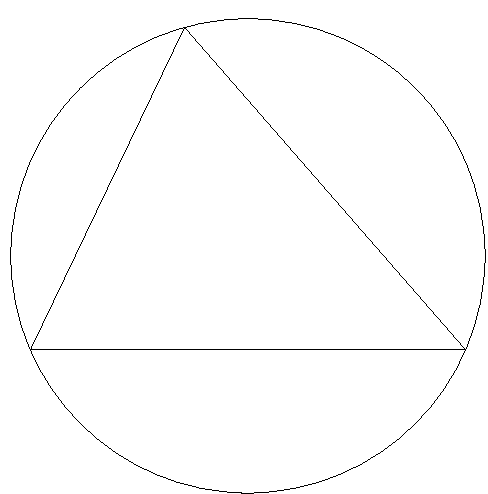
\includegraphics{./Non-isosceles.pdf}%
\end{picture}%
\setlength{\unitlength}{3947sp}%
%
\begingroup\makeatletter\ifx\SetFigFont\undefined%
\gdef\SetFigFont#1#2#3#4#5{%
  \reset@font\fontsize{#1}{#2pt}%
  \fontfamily{#3}\fontseries{#4}\fontshape{#5}%
  \selectfont}%
\fi\endgroup%
\begin{picture}(3888,3949)(2818,-3316)
\put(4152,486){\makebox(0,0)[lb]{\smash{{\SetFigFont{12}{14.4}{\familydefault}{\mddefault}{\updefault}{\color[rgb]{0,0,0}$B$}%
}}}}
\put(2833,-2262){\makebox(0,0)[lb]{\smash{{\SetFigFont{12}{14.4}{\familydefault}{\mddefault}{\updefault}{\color[rgb]{0,0,0}$A$}%
}}}}
\put(6603,-2232){\makebox(0,0)[lb]{\smash{{\SetFigFont{12}{14.4}{\familydefault}{\mddefault}{\updefault}{\color[rgb]{0,0,0}$C$}%
}}}}
\end{picture}%

\end{center}

\end{exer}
\clearpage

\noindent{\large \bf Exercises --- \thesection\ }

\begin{enumerate}
\item Prove that if the cube of an integer is odd, then that integer is odd.

\hint{The best hint for this problem is simply to write down the contrapositive statement. It is trivial to prove!}

\wbvfill

\item Prove that whenever a prime $p$ does not divide the square of an integer, 
it also doesn't divide the original integer. 
($p \nmid x^2 \; \implies \; p \nmid x$)

\hint{The contrapositive is $(p \divides x) \; \implies \; (p \divides x^2)$.}

\wbvfill

\workbookpagebreak

\item Prove (by contradiction) that there is no largest integer.

\hint{Well, if there was a largest integer -- let's call it $L$ (for largest) -- then isn't $L+1$ an integer, and isn't it bigger?  That's the main idea.  A more formal proof might look like this:

\begin{proof} 
Suppose (by way of contradiction) that there is a largest integer $L$.   Then $L \in \Integers$ and $\forall z \in \Integers, L \geq z$.
Consider the quantity $L+1$.  Clearly $L+1$ is an integer (because it is the sum of two integers) and also
$L+1 > L$.   This is a contradiction so the original supposition is false.   Hence there is no largest integer.
\end{proof}
}

\wbvfill

\item Prove (by contradiction) that there is no smallest positive real number.

\hint{Assume there was a smallest positive real number -- might as well call it $s$ (for smallest) -- what can we do to produce an even smaller number? (But be careful that it needs to remain positive -- for instance $s-1$ won't work.)}

\wbvfill

\workbookpagebreak

\item Prove (by contradiction) that the sum of a rational and an irrational 
number is irrational.

\hint{Suppose that x is rational and y is irrational and their sum (let's call it z) is also rational. Do some algebra to solve for y, and you will see that y (which is, by presumption, irrational) is also the difference of two rational numbers (and hence, rational -- a contradiction.)
}

\wbvfill

%\workbookpagebreak

\item Prove (by contraposition) that for all integers $x$ and $y$, if $x+y$ is odd, then $x\neq y$.

\hint{Well, the problem says to do this by contraposition, so let's write down the contrapositive:

\[ \forall x, y \in \Integers, \; x=y \, \implies \, x+y \; \mbox{is even}. \]

But proving that is obvious!
}

\wbvfill

\workbookpagebreak

\item Prove (by contraposition) that for all real numbers $a$ and $b$, if $ab$ is irrational, then $a$
is irrational or $b$ is irrational.

\hint{The contrapositive would be:

\[ \forall a,b \in \Reals, \; (a \in \Rationals \land b \in \Rationals) \, \implies ab \in \Rationals. \]

Wow! Haven't we proved that before?}

\wbvfill


%\workbookpagebreak

\item A \index{Pythagorean triple}\emph{Pythagorean triple} is a set of three
natural numbers, $a$, $b$ and $c$, such that $a^2 + b^2 = c^2$.  Prove that, in a
Pythagorean triple, at least one of $a$ and $b$ is even.  Use either a proof by
contradiction or a proof by contraposition.

\hint{If both $a$ and $b$ are odd then their squares will be 1 mod 4 -- so the sum of their squares
will be 2 mod 4.  But $c^2$ can only be 0 or 1 mod 4, which gives us a contradiction.}

\wbvfill

\workbookpagebreak

\item Suppose you have 2 pairs of positive real numbers whose products are 1.  That is, you have $(a,b)$ and $(c,d)$ in $\Reals^2$ satisfying $ab=cd=1$.  Prove that
$a < c$ implies that $b > d$.

 \hint{
 \begin{proof}
 Suppose by way of contradiction that $a,b,c,d \in \Reals$ satisfy $ab=cd=1$ and that $a<c$ and $b \leq d$.
 By multiplying the inequalities we get that $ab < cd$ which contradicts the assumption that both products
 are equal to 1 (and so must be equal to one another).
 \end{proof} 
  } 
  
  \wbvfill
  
  \workbookpagebreak
  
\end{enumerate}


\newpage

\section{Disproofs}
\label{sec:disproofs}

The idea of a ``disproof'' is really just semantics -- in order to
disprove a statement we need to \emph{prove} its negation.  

So far we've been discussing proofs quite a bit, but have paid
very little attention to a really huge issue.  If the statements
we are attempting to prove are false, no proof is ever going to
be possible.  Really, a prerequisite to developing a facility with
proofs is developing a good ``lie detector.''   We need to be able 
to guess, or quickly ascertain, whether a statement is true or false.
If we are given a universally quantified statement the first thing to
do is try it out for some random elements of the universe we're working
in.  If we happen across a value that satisfies the statement's hypotheses
but doesn't satisfy the conclusion, we've found what is known as a 
\index{counterexample}\emph{counterexample}.  

Consider the following statement about integers and divisibility:

\begin{conj} \label{conj:prim}
\[ \forall a,b,c \in \Integers, \; a \divides bc \; \implies \; a \divides b \,
\lor \, a \divides c. \]
\end{conj}

This is phrased as a UCS, so the hypothesis is clear, we're looking 
for three integers so that the first divides the product of the other
two. In the following table we have collected several values for
$a$, $b$ and $c$ such that $a \divides bc$.

\begin{center}
\begin{tabular}{c|c|c|c}
$a$ & $b$ & $c$ & $ a \divides b \, \lor \, a \divides c $ ? \\ \hline
2 & 7 & 6 & yes \\  
2 & 4 & 5 & yes \\  
3 & 12 & 11 & yes \\
3 & 5 & 15 & yes \\
5 & 4 & 15 & yes \\
5 & 10 & 3 & yes \\
7 & 2 & 14 & yes \\
\end{tabular}
\end{center}

\begin{exer} 
As noted in Section~\ref{sec:def} the statement above is related to
whether or not $a$ is prime.  Note that in the table, only prime
values of $a$ appear.  This is a rather broad hint.  Find a 
counterexample to Conjecture~\ref{conj:prim}.
\end{exer}

There can be times when the search for a counterexample starts to feel
really futile.  Would you think it likely that a statement about
natural numbers could be true for (more than) the first 50 numbers
a yet still be false?  

\begin{conj}
\label{conj:prim2}
\[ \forall n \in \Integers^+ \; n^2 - 79n + 1601 \, \mbox{is prime.} \]
\end{conj}

\begin{exer}
Find a counterexample to Conjecture~\ref{conj:prim2}
\end{exer}

Hidden within Euclid's proof of the infinitude of the primes is
a sequence.  Recall that in the proof we deduced a contradiction
by considering the number $N$ defined by 

\[  N = 1 + \prod_{k=1}^n p_k. \]

Define a sequence by

\[  N_n  = 1 + \prod_{k=1}^n p_k, \]

where $\{p_1, p_2, \ldots , p_n\}$ are the actual first $n$ primes.
The first several values of this sequence are:

\rule{72pt}{0pt} \begin{tabular}{c|c}
 $n$ & $N_n$ \\ \hline
 $1$ & $1+(2) = 3$ \\
 $2$ & $1+(2\cdot 3) = 7$\\
 $3$ & $1+(2\cdot 3\cdot 5) = 31$\\
 $4$ & $1+(2\cdot 3\cdot 5\cdot 7) = 211$\\
 $5$ & $1+(2\cdot 3\cdot 5\cdot 7\cdot 11) = 2311$\\
$\vdots$ & $\vdots$ \\
\end{tabular}

Now, in the proof, we deduced a contradiction by noting that $N_n$ is
much larger than $p_n$, so if $p_n$ is the largest prime it follows that
$N_n$ can't be prime -- but what really appears to be the case (just look 
at that table!) is that $N_n$ actually \emph{is} prime for all $n$. 

\begin{exer}
Find a counterexample to the conjecture that $1+\prod_{k=1}^n p_k$
is itself always a prime.
\end{exer}


\clearpage

\noindent{\large \bf Exercises --- \thesection\ }

\begin{enumerate}
\item Find a polynomial that assumes only prime values for
a reasonably large range of inputs.

\hint{It sort of depends on what is meant by ``a reasonably large range of inputs.''  For example the polynomial $p(x) = 2x+1$ gives primes three times in a row (at $x=1,2$ and $3$).  See if you can do better than that.
}
\item Find a counterexample to \ifthenelse{\boolean{InTextBook}}{Conjecture~\ref{conj:prim}}{the conjecture that $\forall a,b,c \in \Integers, a \divides bc \; \implies \; a \divides b \, \lor \, a \divides c$} using only powers of 2.

\hint{The intent of the problem is that you find three numbers, $a$, $b$ and $c$, that are all powers 
of $2$ and such that $a$ divides the product $bc$, but neither of the factors separately. For instance, 
if you pick $a=16$, then you would need to choose $b$ and $c$ so that $16$ doesn't divide evenly 
into them (they would need to be less than $16$\ldots) but so that their product {\em is} divisible by $16$.
}

\item The alternating sum of factorials provides an interesting
example of a sequence of integers.
\begin{center}
\[ 1! = 1 \]
\[ 2! - 1! = 1\]
\[ 3! - 2! + 1! = 5 \]
\[ 4! - 3! + 2! - 1! = 19 \]
et cetera
\end{center}

\noindent Are they all prime?  (After the first two 1's.)

\hint{

Here's some Sage code that would test this conjecture:

{\tt 
n=1\newline
for i in [2..8]:\newline
    n = factorial(i) - n\newline
    show(factor(n))\newline
}

Of course it turns out that going out to $8$ isn't quite far enough\ldots

}


\item It has been conjectured that whenever $p$ is prime, $2^p - 1$ is
also prime.  Find a minimal counterexample.

\hint{I would definitely seek help at your friendly neighborhood CAS.  In Sage 
you can loop over the first several prime numbers using the following syntax.

{\tt for p in [2,3,5,7,11,13]:}

\noindent If you want to automate that somewhat, there is a Sage function that returns a list
of all the primes in some range.  So the following does the same thing.

{\tt for p in primes(2,13):}


}
\item True or false:  The sum of any two irrational numbers is irrational.
Prove your answer.

\hint{This statement and the next are negations of one another.  Your answers should reflect that.}

\item True of false:  There are two irrational numbers whose sum is rational.
Prove your answer.

\hint{If a number is irrational, isn't its negative also irrational?  That's actually a pretty huge hint.}

\item True or false: The product of any two irrational numbers is irrational.
Prove your answer.

\hint{This one and the next are negations too. Aren't they?}

\item True or false: There are two irrational numbers whose product is rational.
Prove your answer.

\hint{The two numbers {\em could} be equal couldn't they?}

\item True or false:  Whenever an integer $n$ is a divisor of the square of an integer, $m^2$, it follows that $n$ is a divisor of $m$ as well.
(In symbols, $\forall n \in \Integers, \forall m \in \Integers, n \mid m^2 \; \implies \; n \mid m$.)
Prove your answer.

\hint{Hint: List all of the divisors of $36 = (2\cdot 3)^2$.  See if any of them are bigger than $6$.}

\item In an exercise in Section~\ref{sec:more} we proved that the quadratic 
equation $ax^2 + bx + c = 0$ has two solutions if $ac < 0$.  Find a counterexample which shows that this implication cannot be replaced with a biconditional.  

\hint{We'd want $ac$ to be positive (so $a$ and $c$ have the same sign) but nevertheless have $b^2-4ac > 0$.  It seems that if we make $b$ sufficiently large that could happen.}


\end{enumerate}



\newpage
\section[By cases and By exhaustion]{Even more direct proofs: By cases and By exhaustion}
\label{sec:cases}

\index{proof by exhaustion}
Proof by exhaustion is the least attractive proof method from 
an aesthetic perspective.  An exhaustive proof consists of literally
(and exhaustively) checking every element of the universe to see
if the given statement is true for it.  Usually, of course, this is
impossible because the universe of discourse is infinite; but when the
universe of discourse is finite, one certainly can't argue the validity
of an exhaustive proof.  

In the last few decades the introduction of powerful computational
assistance for mathematicians has lead to a funny situation.  There
is a growing list of important results that have been ``proved'' by
exhaustion using a computer.  Important examples of this phenomenon
are the non-existence of a 
\index{projective plane of order 10}
projective plane of order 10\cite{lam} and the 
only known value of a 
\index{Ramsey number}Ramsey number for hypergraphs\cite{radz}. 

\index{proof by cases}
Proof by cases is subtly different from exhaustive proof -- for one 
thing a valid proof by cases can be used in an infinite universe.  
In a proof by cases one has to divide the universe of discourse into
a finite number of sets\footnote{It is necessary to provide an argument that 
this list of cases is complete!  I.e. that every element of the universe
falls into one of the cases.} and then provide a separate proof for each
of the cases.  A great many statements about the integers can be proved
using the division of integers into even and odd.  Another set of 
cases that is used frequently is the finite number of possible remainders
obtained when dividing by an integer $d$.  (Note that even and odd correspond
to the remainders $0$ and $1$ obtained after division by $2$.)    
  
A very famous instance of proof by cases is the computer-assisted proof
of the 
\index{four color theorem}
four color theorem.  The four color theorem is a result known to
map makers for quite some time that says that 4 colors are always sufficient
to color the nations on a map in such a way that countries sharing a boundary
are always colored differently.  Figure~\ref{fig:Lux_map} shows one instance
of an arrangement of nations that requires at least four different colors, 
the theorem says that four colors are \emph{always} enough.  It should be noted
that real cartographers usually reserve a fifth color for oceans (and other 
water) and that it is possible to conceive of a map requiring five colors if 
one allows the nations to be non-contiguous.   In 1977, 
\index{Appel, Kenneth} Kenneth Appel and 
\index{Haken, Wolfgang}Wolfgang Haken proved the four color
theorem by reducing the infinitude of possibilities to 
1,936 separate cases and analyzing each of these with a computer.  
The inelegance of a proof by cases is probably proportional to some power of
the number of cases, but in any case, this proof is generally considered 
somewhat inelegant.  Ever since the proof was announced there has been an
ongoing effort to reduce the number of cases (currently the record is 633
cases -- still far too many to be checked through without a computer) or to
find a proof that does not rely on cases.  For a  good introductory article on
the four color theorem see\cite{wiki-4color}. 

\begin{figure}[!hbtp] 
\begin{center}
\begin{picture}(0,0)%
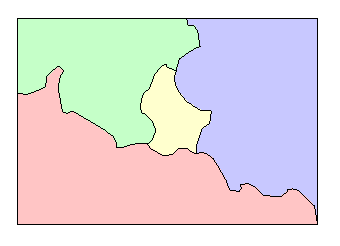
\includegraphics{figures/Luxembourg.pdf}%
\end{picture}%
\setlength{\unitlength}{3947sp}%
%
\begingroup\makeatletter\ifx\SetFigFont\undefined%
\gdef\SetFigFont#1#2#3#4#5{%
  \reset@font\fontsize{#1}{#2pt}%
  \fontfamily{#3}\fontseries{#4}\fontshape{#5}%
  \selectfont}%
\fi\endgroup%
\begin{picture}(2702,1952)(225,-1412)
\end{picture}%

\end{center}
\caption[A four-color map.]{The nations surrounding %
\index{Luxembourg} Luxembourg show %
that sometimes 4 colors are required in cartography.}
\label{fig:Lux_map}
\end{figure}

Most exhaustive proofs of statements that aren't trivial tend to either be (literally) too exhausting or to seem rather contrived.  One example of a situation
in which an exhaustive proof of some statement exists is when the statement
is thought to be universally true but no general proof is known -- yet the
statement has been checked for a large number of cases.  
\index{Goldbach's conjecture}Goldbach's conjecture
is one such statement.  
\index{Goldbach, Christian}Christian Goldbach~\cite{wiki-goldbach} 
was a mathematician born
in \index{K\"{o}nigsberg}K\"{o}nigsberg Prussia, 
who, curiously, did \emph{not} make the
conjecture\footnote{This conjecture was %
discussed previously in the exercises of Section~\ref{sec:def}} which bears
his name.  In a letter to 
\index{Euler, Leonhard}Leonard Euler, Goldbach conjectured that every
odd number greater than 5 could be expressed as the sum of three primes (nowadays this is known as the 
\index{weak Goldbach conjecture} weak Goldbach conjecture).  Euler apparently liked the 
problem and replied to Goldbach stating what is now known as Goldbach's 
conjecture: Every even number greater than 2 can be expressed as the sum of
two primes.  This statement has been lying around since 1742, and a great
many of the world's best mathematicians have made their attempts at proving it
-- to no avail! (Well, actually a lot of progress has been made but the result
still hasn't been proved.)  It's easy to verify the Goldbach conjecture for
relatively small even numbers, so what \emph{has} been done is/are proofs by
exhaustion of Goldbach's conjecture restricted to finite universes. 
As of this writing, the conjecture has been verified to be true of
all even numbers less than $2 \times 10^{17}$.      
 
Whenever an exhaustive proof, or a proof by cases exists for some statement
it is generally felt that a direct proof would be more esthetically pleasing.
If you are in a situation that doesn't admit such a direct proof, you should
at least seek a proof by cases using the minimum possible number of cases.
For example, consider the following theorem and proof.

\begin{thm} $\forall n \in \Integers \; n^2 \;$ is of the form $4k$ or 
$4k+1$ for some $k \in \Integers$.
\end{thm}

\begin{proof}
We will consider the four cases determined by the four
possible residues mod 4.

\begin{itemize}
\item[case i)] If $n \equiv 0 \pmod{4}$ then there is an integer $m$
such that $n = 4m$.  It follows that $n^2 = (4m)^2 = 16m^2$ is of the 
form $4k$ where $k$ is $4m^2$.

\item[case ii)] If $n \equiv 1 \pmod{4}$ then there is an integer $m$
such that $n = 4m+1$.  It follows that $n^2 = (4m+1)^2 = 16m^2 + 8m + 1$ 
is of the form $4k+1$ where $k$ is $4m^2+2m$.

\item[case iii)] If $n \equiv 2 \pmod{4}$ then there is an integer $m$
such that $n = 4m+2$.  It follows that $n^2 = (4m+2)^2 = 16m^2 + 16m + 4$ 
is of the form $4k$ where $k$ is $4m^2+4m+1$.

\item[case iv)] If $n \equiv 3 \pmod{4}$ then there is an integer $m$
such that $n = 4m+3$.  It follows that $n^2 = (4m+3)^2 = 16m^2 + 24m + 9$ 
is of the form $4k+1$ where $k$ is $4m^2+6m+2$.
\end{itemize}

Since these four cases exhaust the possibilities and since the desired
result holds in each case, our proof is complete.

\end{proof} 

While the proof just stated is certainly valid, the argument is inelegant
since a smaller number of cases would suffice.

\begin{exer}
The previous theorem can be proved using just two cases.  Do so.
\end{exer}

We'll close this section by asking you to determine an exhaustive proof where 
the complexity of the argument is challenging but not \emph{too} impossible.

\index{graph pebbling} Graph pebbling is an interesting concept originated 
by the famous combinatorialist \index{Chung, Fan} Fan Chung.  A ``graph'' 
(as the term is used here) is a collection
of places or locations which are known as ``nodes,'' some of which 
are joined by paths or connections which are known as ``edges.'' 
Graphs have been studied by mathematicians for about 400 years, and 
many interesting problems can be put in this setting.  Graph pebbling
is a crude version of a broader problem in resource management -- often
a resource actually gets used in the process of transporting it.  Think of
the big tanker trucks that are used to transport gasoline.  What do they
run on?  Well, actually they probably burn diesel --- but the point is
that in order to move the fuel around we have to consume some of it.
Graph pebbling takes this to an extreme: in order to move one pebble
we must consume one pebble.  

Imagine that a bunch of pebbles are randomly
distributed on the nodes of a graph, and that we are allowed to do 
\emph{graph pebbling moves} -- we remove two pebbles from some node
and place a single pebble on a node that is connected to it.
See Figure~\ref{fig:pebbling_move}.

\begin{figure}[!hbtp] 
\begin{center}
\begin{picture}(0,0)%
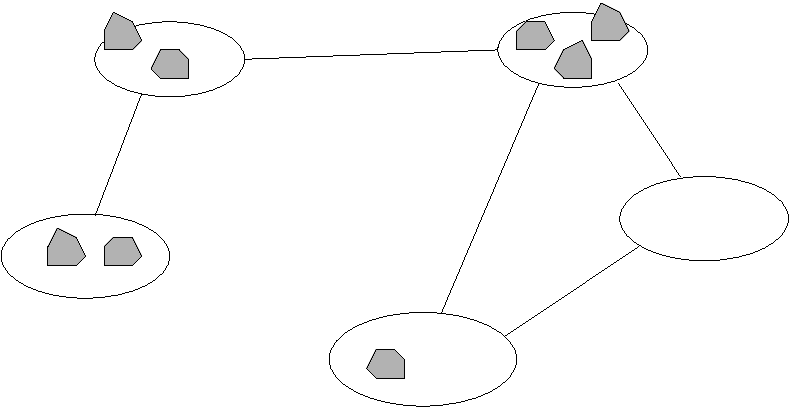
\includegraphics{figures/pebbling.pdf}%
\end{picture}%
\setlength{\unitlength}{3947sp}%
%
\begingroup\makeatletter\ifx\SetFigFont\undefined%
\gdef\SetFigFont#1#2#3#4#5{%
  \reset@font\fontsize{#1}{#2pt}%
  \fontfamily{#3}\fontseries{#4}\fontshape{#5}%
  \selectfont}%
\fi\endgroup%
\begin{picture}(6326,3252)(1268,-2776)
\put(5401,-2761){\makebox(0,0)[lb]{\smash{{\SetFigFont{12}{14.4}{\familydefault}{\mddefault}{\updefault}{\color[rgb]{0,0,0}E}%
}}}}
\put(2701,-1711){\makebox(0,0)[lb]{\smash{{\SetFigFont{12}{14.4}{\familydefault}{\mddefault}{\updefault}{\color[rgb]{0,0,0}A}%
}}}}
\put(3151,-361){\makebox(0,0)[lb]{\smash{{\SetFigFont{12}{14.4}{\familydefault}{\mddefault}{\updefault}{\color[rgb]{0,0,0}B}%
}}}}
\put(6526,-211){\makebox(0,0)[lb]{\smash{{\SetFigFont{12}{14.4}{\familydefault}{\mddefault}{\updefault}{\color[rgb]{0,0,0}C}%
}}}}
\put(7426,-1711){\makebox(0,0)[lb]{\smash{{\SetFigFont{12}{14.4}{\familydefault}{\mddefault}{\updefault}{\color[rgb]{0,0,0}D}%
}}}}
\end{picture}%

\end{center}
\caption[Graph pebbling.]{In graph pebbling problems a collection of pebbles
are distributed on the nodes of a graph.  There is no significance to the 
particular graph that is shown here, or to the arrangement of pebbles -- 
we are just giving an example.}
\label{fig:pebbling}
\end{figure}

\begin{figure}[!hbtp] 
\begin{center}
\begin{picture}(0,0)%
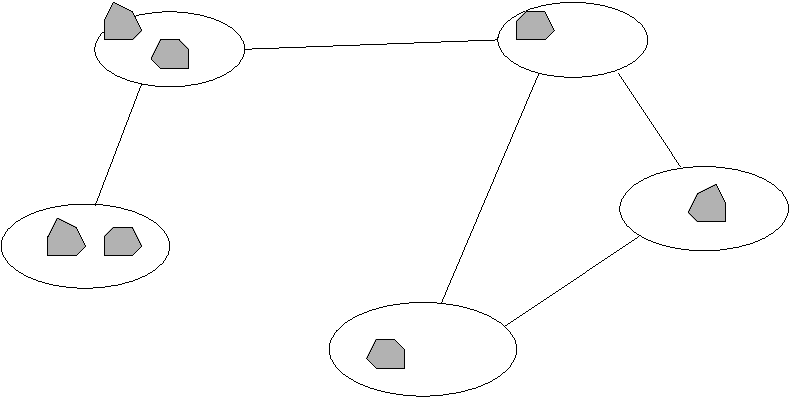
\includegraphics{./pebbling_move.pdf}%
\end{picture}%
\setlength{\unitlength}{3947sp}%
%
\begingroup\makeatletter\ifx\SetFigFont\undefined%
\gdef\SetFigFont#1#2#3#4#5{%
  \reset@font\fontsize{#1}{#2pt}%
  \fontfamily{#3}\fontseries{#4}\fontshape{#5}%
  \selectfont}%
\fi\endgroup%
\begin{picture}(6326,3177)(1268,-2776)
\put(5401,-2761){\makebox(0,0)[lb]{\smash{{\SetFigFont{12}{14.4}{\familydefault}{\mddefault}{\updefault}{\color[rgb]{0,0,0}E}%
}}}}
\put(2701,-1711){\makebox(0,0)[lb]{\smash{{\SetFigFont{12}{14.4}{\familydefault}{\mddefault}{\updefault}{\color[rgb]{0,0,0}A}%
}}}}
\put(3151,-361){\makebox(0,0)[lb]{\smash{{\SetFigFont{12}{14.4}{\familydefault}{\mddefault}{\updefault}{\color[rgb]{0,0,0}B}%
}}}}
\put(6526,-211){\makebox(0,0)[lb]{\smash{{\SetFigFont{12}{14.4}{\familydefault}{\mddefault}{\updefault}{\color[rgb]{0,0,0}C}%
}}}}
\put(7426,-1711){\makebox(0,0)[lb]{\smash{{\SetFigFont{12}{14.4}{\familydefault}{\mddefault}{\updefault}{\color[rgb]{0,0,0}D}%
}}}}
\end{picture}%

\end{center}
\caption[Graph pebbling move.]{A graph pebbling move takes two pebbles off
of a node and puts one of them on an adjacent node (the other is discarded).
Notice how node C, which formerly held 3 pebbles, now has only 1 and that 
a pebble is now present on node D where previously there was none.}
\label{fig:pebbling_move}
\end{figure}

For any particular graph, we can ask for its \emph{pebbling number}, $\rho$.  
This is the smallest number so that if $\rho$ pebbles are distributed {\em in any way whatsoever} on the nodes of the graph, it will be possible to use 
pebbling moves so as to get a pebble to any node. 

For example, consider the triangle graph -- three nodes which are all 
mutually connected.  The pebbling number of this graph is 3.  If we
start with one pebble on each node we are already done; if there is a 
node that has two pebbles on it, we can use a pebbling move to reach
either of the other two nodes.

\begin{exer} 
There is a graph $C_5$ which consists of 5 nodes connected in a circular
fashion.  Determine its pebbling number.  Prove your answer exhaustively.

Hint: the pebbling number must be greater than 4 because if one pebble is
placed on each of 4 nodes the configuration is unmovable (we need to 
have two pebbles on a node in order to be able to make a pebbling move
at all) and so the 5th node can never be reached.
\end{exer}
 
\clearpage

\noindent{\large \bf Exercises --- \thesection\ }

\begin{enumerate}
\item Prove that if $n$ is an odd number then $n^4 \pmod{16} = 1$.

\hint{

While one could perform fairly complicated arithmetic, expanding expression like
$(16k+13)^4$ and then regrouping to put it in the form $16q+1$ (and one would need 
to do that work for each of the odd remainders modulo $16$),  that would be missing out
on the true power of modular notation.  In a ``$\pmod{16}$'' calculation one can simply ignore
summands like $16k$ because they are $0 \pmod{16}$.  Thus, for example,

  \[ (16k+7)^4 \pmod{16} \; = \; 7^4 \pmod{16} \; = \; 2401 \pmod{16}  \; = \; 1. \]
  
So, essentially one just needs to compute the $4$th powers of $1, 3, 5, 7, 9, 11, 13$  and $15$, and
then reduce them modulo 16.  An even greater economy is possible if one notes that (modulo 16) many
of those cases are negatives of one another -- so their $4$th powers are equal.
}

\wbvfill
     
\item Prove that every prime number other than 2 and 3 has the form
$6q+1$ or $6q+5$ for some integer $q$.  (Hint: this problem involves
thinking about cases as well as contrapositives.)

\hint{It is probably obvious that the "cases" will be the possible remainders mod 6. Numbers of the form 6q+0 will be multiples of 6, so clearly not prime. The other forms that need to be eliminated are 6q+2, 6q+3, and 6q+4.
}

\wbvfill

\workbookpagebreak

\item Show that the sum of any three consecutive integers is divisible
by 3.

\hint{Write the sum as $n + (n+1) + (n+2)$.}

\wbvfill

\item There is a graph known as $K_4$ that has $4$ nodes and there is an edge between every pair of nodes.
The pebbling number of $K_4$ has to be at least $4$ since it would be possible to put one pebble on each of
$3$ nodes and not be able to reach the remaining node using pebbling moves.  Show that the pebbling number of $K_4$ is actually $4$.

\hint{If there are two pebbles on any node we will be able to reach all the other nodes using pebbling moves
(since every pair of nodes is connected).}

\wbvfill

\workbookpagebreak

\item Find the pebbling number of a graph whose nodes are the corners and 
whose edges are the, uhmm, edges of a cube.

\hint{It should be clear that the pebbling number is at least $8$ -- $7$ pebbles could be distributed, 
one to a node, and the $8$th node would be unreachable.  It will be easier to play around with this if
you figure out how to draw the cube graph ``flattened-out'' in the plane.}

\wbvfill

\item A \index{vampire number}\emph{vampire number} is a $2n$ digit number $v$ that factors as $v=xy$
where $x$ and $y$ are $n$ digit numbers and the digits of $v$ are the 
union of the digits in $x$ and $y$ in some order.  The numbers $x$ and $y$
are known as the ``fangs'' of $v$.  To eliminate trivial
cases, pairs of trailing zeros are disallowed.  

Show that there are no 2-digit vampire numbers.

Show that there are seven 4-digit vampire numbers.

\hint{The 2-digit challenge is do-able by hand (just barely).  The $4$ digit question certainly requires 
some computer assistance!}

\wbvfill

\workbookpagebreak

\item Lagrange's theorem on representation of integers as sums of squares
says that every positive integer can be expressed as the sum of at most 
$4$ squares.  For example, $79 = 7^2 + 5^2 + 2^2 + 1^2$.  Show (exhaustively) 
that $15$ can not be represented using fewer than $4$ squares.

\hint{Note that $15 = 3^2 + 2^2 + 1^2 + 1^2$.  Also, if $15$ were expressible as a sum of fewer than $4$ squares, the squares involved would be $1$, $4$ and $9$.  It's really not that hard to try all the possibilities.}

\wbvfill

\item Show that there are exactly $15$ numbers $x$ in the range $1 \leq x \leq 100$ that can't be represented using fewer than $4$ squares.



\hint{The following Sage code generates all the numbers up to $100$ that {\em can} be written
as the sum of at most $3$ squares.

{\tt
var('x y z') \newline
a=[s$\caret$2 for s in [1..10]]  \newline
b=[s$\caret$2 for s in [0..10]]  \newline
s = []  \newline
for x in a:  \newline
\tab for y in b:  \newline
\tab \tab for z in b:  \newline
\tab \tab \tab s = union(s,[x+y+z])  \newline
s = Set(s)  \newline
H=Set([1..100]) \newline
show(H.intersection(s))  \newline
}
}

\wbvfill

\workbookpagebreak

\item The \index{trichotomy property}\emph{trichotomy property} of the real 
numbers simply states that every real number is either positive or negative 
or zero.  Trichotomy can be used to prove many statements by looking at the
three cases that it guarantees.  Develop a proof (by cases) that the square of
any real number is non-negative.

\hint{By trichotomy, x is either zero, negative, or positive. If x is zero, its square is zero. If x is negative, its square is positive. If x is positive, its square is also positive.}

\wbvfill

\item Consider the game called ``binary determinant tic-tac-toe''\footnote{ %
This question was problem A4 in the 63rd annual %
\index{William Lowell Putnam Mathematics Competition} %
William Lowell Putnam Mathematics Competition (2002).  %
There are three collections of questions %
and answers  from previous Putnam exams available from the MAA % 
\cite{putnam1,putnam2,putnam3}% 
}
which is played by two players who alternately fill in the entries of a 
$3 \times 3$ array.  Player One goes first, placing 1's in the array and 
player Zero goes second, placing 0's.  Player One's goal is that the 
final array have determinant 1, and player Zero's goal is that the 
determinant be 0.  The determinant calculations are carried out mod 2.

Show that player Zero can always win a game of binary determinant tic-tac-toe
by the method of exhaustion.

\hint{If you know something about determinants it would help here.  The determinant will be
0 if there are two identical rows (or columns) in the finished array.  Also, if there is a row or column
that is all zeros, player Zero wins too.  Also, cyclically permuting either rows or columns has no effect
on the determinant of a binary array.  This means we lose no generality in assuming player One's
first move goes (say) in the upper-left corner.}

\wbvfill

\workbookpagebreak

\rule{0pt}{0pt}

\workbookpagebreak

\end{enumerate}



\newpage

\section[Existential statements]{Proofs and disproofs of existential statements}
\label{sec:exist}

From a certain point of view, there is no need for the current section.
If we are proving an existential statement we are \emph{disproving} some
universal statement. (Which has already been discussed.)  Similarly,
if we are trying to disprove an existential statement, then we are
actually \emph{proving} a related universal statement.  Nevertheless,
sometimes the way a theorem is stated emphasizes the existence question
over the corresponding universal -- and so people talk about proving
and disproving existential statements as a separate issue from 
universal statements.

Proofs of existential questions come in two basic varieties: constructive
and non-constructive.  Constructive proofs are conceptually the easier
of the two -- you actually name an example that shows the existential
question is true.  For example:

\begin{thm}
There is an even prime.
\end{thm}

\begin{proof}
The number 2 is both even and prime. 
\end{proof} 

\begin{exer}
The Fibonacci numbers are defined by the initial values $F(0)=1$
and $F(1)=1$ and the recursive formula $F(n+1) = F(n)+F(n-1)$ (to
get the next number in the series you add the last and the penultimate).

\rule{72pt}{0pt} \begin{tabular}{c|c}
$n$ & $F(n)$ \\ \hline
0 & 1 \\
1 & 1 \\
2 & 2 \\
3 & 3 \\
4 & 5 \\
5 & 8 \\
$\vdots$ & $\vdots$\\
\end{tabular}
\medskip

Prove that there is a Fibonacci number that is a perfect square.
\end{exer}

A non-constructive existence proof is trickier.  One approach is to argue
by contradiction -- if the thing we're seeking doesn't exist that will
lead to an absurdity.  Another approach is to outline a search algorithm
for the desired item and provide an argument as to why it cannot fail!

A particularly neat approach is to argue using dilemma.
This is my favorite non-constructive existential theorem/proof.

\begin{thm}
There are irrational numbers $\alpha$ and $\beta$ such that $\alpha^\beta$
is rational.
\end{thm}

\begin{proof}
If $\sqrt{2}^{\sqrt{2}}$ is rational then we are done.
(Let $ \alpha = \beta = \sqrt{2}$.)  Otherwise, let 
$\alpha = \sqrt{2}^{\sqrt{2}}$ and $\beta = \sqrt{2}$.  The result
follows because $\left(\sqrt{2}^{\sqrt{2}}\right)^{\sqrt{2}} = \sqrt{2}^{(\sqrt{2}\sqrt{2})} 
= \sqrt{2}^2 = 2$, which is clearly rational.

\end{proof} 

Many existential proofs involve a property of the natural numbers
known as the \index{well-ordering principle}well-ordering principle.  The well-ordering principle is 
sometimes abbreviated WOP.  If a set has WOP it doesn't mean that the 
set is ordered in a particularly good way, but rather that its subsets
are like wells -- the kind one hoists water out of with a bucket on a rope.
You needn't be concerned with WOP in general at this point, but notice
that the subsets of the natural numbers have a particularly nice property
 -- any non-empty set of natural numbers must have a least element (much like
every water well has a bottom).

Because the natural numbers have the well-ordering principle 
we can prove that there is a least 
natural number with property X by simply finding \emph{any} natural
number with property X -- by doing that we've shown that the set of
natural numbers with property X is non-empty and that's the only
hypothesis the WOP needs.  

For example, in the exercises in Section~\ref{sec:cases} we 
introduced vampire numbers. A \index{vampire number} \emph{vampire number} 
is a 
$2n$ digit number $v$ that factors as $v=xy$
where $x$ and $y$ are $n$ digit numbers and the digits of $v$ are precisely the digits in $x$ and $y$ in some order.  The numbers $x$ and $y$
are known as the ``fangs'' of $v$.  To eliminate trivial
cases, both fangs may not end with zeros.  


\begin{thm}
There is a smallest 6-digit vampire number.
\end{thm}

\begin{proof}
The number $125460$ is a vampire number (in fact this is the smallest
example of a vampire number with two sets of fangs: 
$125460 = 204\cdot 615 = 246\cdot 510$).  Since the set of 6-digit vampire
numbers is non-empty, the well-ordering principle of the natural numbers
allows us to deduce that there is a smallest 6-digit vampire number.
\end{proof} 
 
This is quite an interesting situation in that we know there is a smallest
6-digit vampire number without having any idea what it is!

\begin{exer}
Show that $102510$ is the smallest 6-digit vampire number.
\end{exer}

There are quite a few occasions when we need to prove statements
involving the \index{unique existence} unique existence quantifier 
($\exists !$).  In
such instances we need to do just a little bit more work.  We
need to show existence -- either constructively or non-constructively --
and we also need to show uniqueness.  To give an example of 
a unique existence proof we'll return to a concept first
discussed in Section~\ref{sec:alg} and finish-up some business
that was glossed-over there.

Recall the Euclidean algorithm that was used to calculate the 
\index{greatest common divisor, gcd}greatest
common divisor of two integers $a$ and $b$ (which we denote $\gcd{a}{b}$).
There is a rather important question concerning algorithms known as
the ``halting problem.''  Does the program eventually halt, or does it get 
stuck in an infinite loop?  We know that the Euclidean algorithm halts
(and outputs the correct result) because we know the following
unique existence result.

\[ \forall a, b \in \Integers^+, \, \exists ! \, d \in \Integers^+ \; \mbox{such that} \, d=\gcd{a}{b} \]
  
Now, before we can prove this result, we'll need a precise definition
for $\gcd{a}{b}$.   Firstly, a gcd must be a \emph{common divisor} which
means it needs to divide both $a$ and $b$.  Secondly, among all the common 
divisors, it must be the \emph{largest}.  This second point is usually 
addressed
by requiring that every other common divisor divides the gcd. Finally we 
should note that a gcd is always positive, for whenever a number divides
another number so does its negative, and whichever of those two is positive
will clearly be the greater!  This allows us to extend the definition of
gcd to all integers, but things are conceptually easier if we 
keep our attention restricted to the positive integers. 

\begin{defi}
The \emph{greatest common divisor}, or gcd, of two positive 
integers $a$ and $b$
is a positive integer $d$ such that $d \divides a$ and $d \divides b$ and if $c$ is any
other positive integer such that $c \divides a$ and $c \divides b$ then $c \divides d$.
  
\[ \forall a,b,c,d \in \Integers^+ \; d=\gcd{a}{b} \; \iff \;
d \divides a \, \land \, d \divides b \, \land \, (c \divides a \, \land \, c \divides b  \implies c \divides d)\]
\end{defi}

Armed with this definition, let's return our attention to proving the
unique existence of the gcd.  The uniqueness part is easier so we'll
do that first.  We argue by contradiction.  Suppose that there were
two different numbers $d$ and $d'$ satisfying the definition of $\gcd{a}{b}$.
Put $d'$ in the place of $c$ in the definition to see that $d' \divides d$.
Similarly, we can deduce that $d \divides d'$ and if two numbers each divide 
into the other, they must be equal.  This is a contradiction since we
assumed $d$ and $d'$ were different.

For the existence part we'll need to define a set -- known as the 
\index{Z-module}$\Integers$-module generated by $a$ and $b$ -- that consists of all 
numbers of the form $xa+yb$ where $x$ and $y$ range over the integers.

\begin{figure}[!hbtp] 
\begin{center}
\begin{picture}(0,0)%
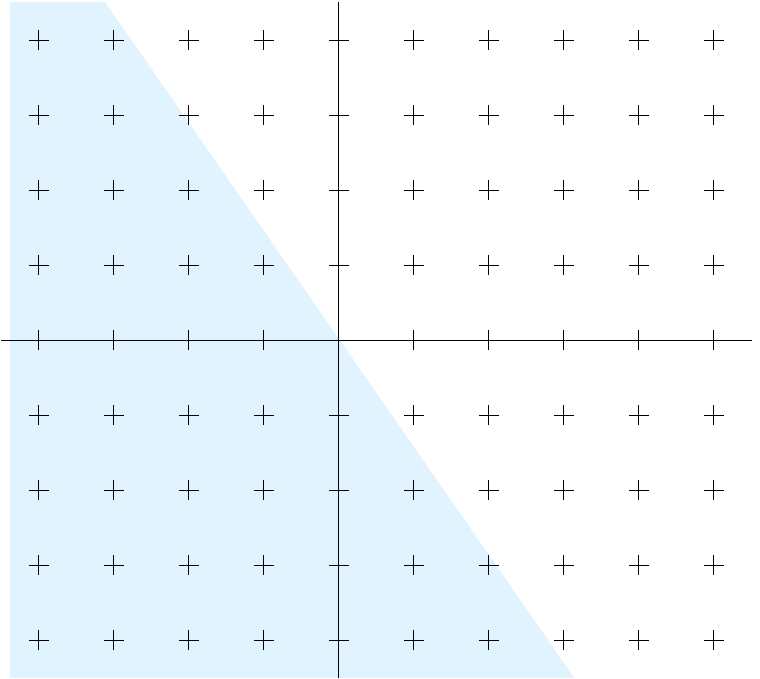
\includegraphics{figures/Z-module.pdf}%
\end{picture}%
\setlength{\unitlength}{3947sp}%
%
\begingroup\makeatletter\ifx\SetFigFont\undefined%
\gdef\SetFigFont#1#2#3#4#5{%
  \reset@font\fontsize{#1}{#2pt}%
  \fontfamily{#3}\fontseries{#4}\fontshape{#5}%
  \selectfont}%
\fi\endgroup%
\begin{picture}(6078,5424)(2089,-5473)
\put(4876,-2086){\makebox(0,0)[lb]{\smash{{\SetFigFont{12}{14.4}{\familydefault}{\mddefault}{\updefault}{\color[rgb]{0,0,0}15}%
}}}}
\put(5476,-2686){\makebox(0,0)[lb]{\smash{{\SetFigFont{12}{14.4}{\familydefault}{\mddefault}{\updefault}{\color[rgb]{0,0,0}21}%
}}}}
\put(5476,-2086){\makebox(0,0)[lb]{\smash{{\SetFigFont{12}{14.4}{\familydefault}{\mddefault}{\updefault}{\color[rgb]{0,0,0}36}%
}}}}
\put(6076,-2686){\makebox(0,0)[lb]{\smash{{\SetFigFont{12}{14.4}{\familydefault}{\mddefault}{\updefault}{\color[rgb]{0,0,0}42}%
}}}}
\put(6676,-2686){\makebox(0,0)[lb]{\smash{{\SetFigFont{12}{14.4}{\familydefault}{\mddefault}{\updefault}{\color[rgb]{0,0,0}63}%
}}}}
\put(7276,-2686){\makebox(0,0)[lb]{\smash{{\SetFigFont{12}{14.4}{\familydefault}{\mddefault}{\updefault}{\color[rgb]{0,0,0}84}%
}}}}
\put(7876,-2686){\makebox(0,0)[lb]{\smash{{\SetFigFont{12}{14.4}{\familydefault}{\mddefault}{\updefault}{\color[rgb]{0,0,0}105}%
}}}}
\put(4276,-2686){\makebox(0,0)[lb]{\smash{{\SetFigFont{12}{14.4}{\familydefault}{\mddefault}{\updefault}{\color[rgb]{0,0,0}-21}%
}}}}
\put(3676,-2686){\makebox(0,0)[lb]{\smash{{\SetFigFont{12}{14.4}{\familydefault}{\mddefault}{\updefault}{\color[rgb]{0,0,0}-42}%
}}}}
\put(3076,-2686){\makebox(0,0)[lb]{\smash{{\SetFigFont{12}{14.4}{\familydefault}{\mddefault}{\updefault}{\color[rgb]{0,0,0}-63}%
}}}}
\put(2476,-2686){\makebox(0,0)[lb]{\smash{{\SetFigFont{12}{14.4}{\familydefault}{\mddefault}{\updefault}{\color[rgb]{0,0,0}-84}%
}}}}
\put(4876,-3286){\makebox(0,0)[lb]{\smash{{\SetFigFont{12}{14.4}{\familydefault}{\mddefault}{\updefault}{\color[rgb]{0,0,0}-15}%
}}}}
\put(4876,-3886){\makebox(0,0)[lb]{\smash{{\SetFigFont{12}{14.4}{\familydefault}{\mddefault}{\updefault}{\color[rgb]{0,0,0}-30}%
}}}}
\put(4876,-4486){\makebox(0,0)[lb]{\smash{{\SetFigFont{12}{14.4}{\familydefault}{\mddefault}{\updefault}{\color[rgb]{0,0,0}-45}%
}}}}
\put(4876,-5086){\makebox(0,0)[lb]{\smash{{\SetFigFont{12}{14.4}{\familydefault}{\mddefault}{\updefault}{\color[rgb]{0,0,0}-60}%
}}}}
\put(4876,-1486){\makebox(0,0)[lb]{\smash{{\SetFigFont{12}{14.4}{\familydefault}{\mddefault}{\updefault}{\color[rgb]{0,0,0}30}%
}}}}
\put(4876,-886){\makebox(0,0)[lb]{\smash{{\SetFigFont{12}{14.4}{\familydefault}{\mddefault}{\updefault}{\color[rgb]{0,0,0}45}%
}}}}
\put(4876,-286){\makebox(0,0)[lb]{\smash{{\SetFigFont{12}{14.4}{\familydefault}{\mddefault}{\updefault}{\color[rgb]{0,0,0}60}%
}}}}
\put(5476,-1486){\makebox(0,0)[lb]{\smash{{\SetFigFont{12}{14.4}{\familydefault}{\mddefault}{\updefault}{\color[rgb]{0,0,0}51}%
}}}}
\put(5476,-886){\makebox(0,0)[lb]{\smash{{\SetFigFont{12}{14.4}{\familydefault}{\mddefault}{\updefault}{\color[rgb]{0,0,0}66}%
}}}}
\put(5476,-286){\makebox(0,0)[lb]{\smash{{\SetFigFont{12}{14.4}{\familydefault}{\mddefault}{\updefault}{\color[rgb]{0,0,0}81}%
}}}}
\put(4876,-2686){\makebox(0,0)[lb]{\smash{{\SetFigFont{12}{14.4}{\familydefault}{\mddefault}{\updefault}{\color[rgb]{0,0,0}0}%
}}}}
\put(4276,-3286){\makebox(0,0)[lb]{\smash{{\SetFigFont{12}{14.4}{\familydefault}{\mddefault}{\updefault}{\color[rgb]{0,0,0}-36}%
}}}}
\put(4276,-3886){\makebox(0,0)[lb]{\smash{{\SetFigFont{12}{14.4}{\familydefault}{\mddefault}{\updefault}{\color[rgb]{0,0,0}-51}%
}}}}
\put(4276,-4486){\makebox(0,0)[lb]{\smash{{\SetFigFont{12}{14.4}{\familydefault}{\mddefault}{\updefault}{\color[rgb]{0,0,0}-66}%
}}}}
\put(4276,-5086){\makebox(0,0)[lb]{\smash{{\SetFigFont{12}{14.4}{\familydefault}{\mddefault}{\updefault}{\color[rgb]{0,0,0}-81}%
}}}}
\put(6076,-2086){\makebox(0,0)[lb]{\smash{{\SetFigFont{12}{14.4}{\familydefault}{\mddefault}{\updefault}{\color[rgb]{0,0,0}57}%
}}}}
\put(6076,-1486){\makebox(0,0)[lb]{\smash{{\SetFigFont{12}{14.4}{\familydefault}{\mddefault}{\updefault}{\color[rgb]{0,0,0}72}%
}}}}
\put(6076,-886){\makebox(0,0)[lb]{\smash{{\SetFigFont{12}{14.4}{\familydefault}{\mddefault}{\updefault}{\color[rgb]{0,0,0}87}%
}}}}
\put(6076,-286){\makebox(0,0)[lb]{\smash{{\SetFigFont{12}{14.4}{\familydefault}{\mddefault}{\updefault}{\color[rgb]{0,0,0}102}%
}}}}
\put(6676,-2086){\makebox(0,0)[lb]{\smash{{\SetFigFont{12}{14.4}{\familydefault}{\mddefault}{\updefault}{\color[rgb]{0,0,0}78}%
}}}}
\put(6676,-1486){\makebox(0,0)[lb]{\smash{{\SetFigFont{12}{14.4}{\familydefault}{\mddefault}{\updefault}{\color[rgb]{0,0,0}93}%
}}}}
\put(6676,-886){\makebox(0,0)[lb]{\smash{{\SetFigFont{12}{14.4}{\familydefault}{\mddefault}{\updefault}{\color[rgb]{0,0,0}108}%
}}}}
\put(6676,-286){\makebox(0,0)[lb]{\smash{{\SetFigFont{12}{14.4}{\familydefault}{\mddefault}{\updefault}{\color[rgb]{0,0,0}123}%
}}}}
\put(7276,-2086){\makebox(0,0)[lb]{\smash{{\SetFigFont{12}{14.4}{\familydefault}{\mddefault}{\updefault}{\color[rgb]{0,0,0}99}%
}}}}
\put(7276,-1486){\makebox(0,0)[lb]{\smash{{\SetFigFont{12}{14.4}{\familydefault}{\mddefault}{\updefault}{\color[rgb]{0,0,0}114}%
}}}}
\put(7276,-886){\makebox(0,0)[lb]{\smash{{\SetFigFont{12}{14.4}{\familydefault}{\mddefault}{\updefault}{\color[rgb]{0,0,0}129}%
}}}}
\put(7276,-286){\makebox(0,0)[lb]{\smash{{\SetFigFont{12}{14.4}{\familydefault}{\mddefault}{\updefault}{\color[rgb]{0,0,0}144}%
}}}}
\put(7876,-2086){\makebox(0,0)[lb]{\smash{{\SetFigFont{12}{14.4}{\familydefault}{\mddefault}{\updefault}{\color[rgb]{0,0,0}120}%
}}}}
\put(7876,-1486){\makebox(0,0)[lb]{\smash{{\SetFigFont{12}{14.4}{\familydefault}{\mddefault}{\updefault}{\color[rgb]{0,0,0}135}%
}}}}
\put(7876,-886){\makebox(0,0)[lb]{\smash{{\SetFigFont{12}{14.4}{\familydefault}{\mddefault}{\updefault}{\color[rgb]{0,0,0}150}%
}}}}
\put(7876,-286){\makebox(0,0)[lb]{\smash{{\SetFigFont{12}{14.4}{\familydefault}{\mddefault}{\updefault}{\color[rgb]{0,0,0}165}%
}}}}
\put(5476,-3286){\makebox(0,0)[lb]{\smash{{\SetFigFont{12}{14.4}{\familydefault}{\mddefault}{\updefault}{\color[rgb]{0,0,0}6}%
}}}}
\put(6076,-3286){\makebox(0,0)[lb]{\smash{{\SetFigFont{12}{14.4}{\familydefault}{\mddefault}{\updefault}{\color[rgb]{0,0,0}27}%
}}}}
\put(6676,-3286){\makebox(0,0)[lb]{\smash{{\SetFigFont{12}{14.4}{\familydefault}{\mddefault}{\updefault}{\color[rgb]{0,0,0}48}%
}}}}
\put(7276,-3286){\makebox(0,0)[lb]{\smash{{\SetFigFont{12}{14.4}{\familydefault}{\mddefault}{\updefault}{\color[rgb]{0,0,0}69}%
}}}}
\put(7876,-3286){\makebox(0,0)[lb]{\smash{{\SetFigFont{12}{14.4}{\familydefault}{\mddefault}{\updefault}{\color[rgb]{0,0,0}90}%
}}}}
\put(5476,-3886){\makebox(0,0)[lb]{\smash{{\SetFigFont{12}{14.4}{\familydefault}{\mddefault}{\updefault}{\color[rgb]{0,0,0}-9}%
}}}}
\put(6076,-3886){\makebox(0,0)[lb]{\smash{{\SetFigFont{12}{14.4}{\familydefault}{\mddefault}{\updefault}{\color[rgb]{0,0,0}12}%
}}}}
\put(6676,-3886){\makebox(0,0)[lb]{\smash{{\SetFigFont{12}{14.4}{\familydefault}{\mddefault}{\updefault}{\color[rgb]{0,0,0}33}%
}}}}
\put(7276,-3886){\makebox(0,0)[lb]{\smash{{\SetFigFont{12}{14.4}{\familydefault}{\mddefault}{\updefault}{\color[rgb]{0,0,0}54}%
}}}}
\put(7876,-3886){\makebox(0,0)[lb]{\smash{{\SetFigFont{12}{14.4}{\familydefault}{\mddefault}{\updefault}{\color[rgb]{0,0,0}75}%
}}}}
\put(4276,-2086){\makebox(0,0)[lb]{\smash{{\SetFigFont{12}{14.4}{\familydefault}{\mddefault}{\updefault}{\color[rgb]{0,0,0}-6}%
}}}}
\put(3676,-2086){\makebox(0,0)[lb]{\smash{{\SetFigFont{12}{14.4}{\familydefault}{\mddefault}{\updefault}{\color[rgb]{0,0,0}-27}%
}}}}
\put(3076,-2086){\makebox(0,0)[lb]{\smash{{\SetFigFont{12}{14.4}{\familydefault}{\mddefault}{\updefault}{\color[rgb]{0,0,0}-48}%
}}}}
\put(4276,-1486){\makebox(0,0)[lb]{\smash{{\SetFigFont{12}{14.4}{\familydefault}{\mddefault}{\updefault}{\color[rgb]{0,0,0}9}%
}}}}
\put(3676,-1486){\makebox(0,0)[lb]{\smash{{\SetFigFont{12}{14.4}{\familydefault}{\mddefault}{\updefault}{\color[rgb]{0,0,0}-12}%
}}}}
\put(3076,-1486){\makebox(0,0)[lb]{\smash{{\SetFigFont{12}{14.4}{\familydefault}{\mddefault}{\updefault}{\color[rgb]{0,0,0}-33}%
}}}}
\put(4276,-886){\makebox(0,0)[lb]{\smash{{\SetFigFont{12}{14.4}{\familydefault}{\mddefault}{\updefault}{\color[rgb]{0,0,0}24}%
}}}}
\put(3676,-886){\makebox(0,0)[lb]{\smash{{\SetFigFont{12}{14.4}{\familydefault}{\mddefault}{\updefault}{\color[rgb]{0,0,0}3}%
}}}}
\put(2476,-1486){\makebox(0,0)[lb]{\smash{{\SetFigFont{12}{14.4}{\familydefault}{\mddefault}{\updefault}{\color[rgb]{0,0,0}-54}%
}}}}
\put(2476,-3286){\makebox(0,0)[lb]{\smash{{\SetFigFont{12}{14.4}{\familydefault}{\mddefault}{\updefault}{\color[rgb]{0,0,0}-99}%
}}}}
\put(3076,-3286){\makebox(0,0)[lb]{\smash{{\SetFigFont{12}{14.4}{\familydefault}{\mddefault}{\updefault}{\color[rgb]{0,0,0}-78}%
}}}}
\put(3676,-3286){\makebox(0,0)[lb]{\smash{{\SetFigFont{12}{14.4}{\familydefault}{\mddefault}{\updefault}{\color[rgb]{0,0,0}-57}%
}}}}
\put(2476,-3886){\makebox(0,0)[lb]{\smash{{\SetFigFont{12}{14.4}{\familydefault}{\mddefault}{\updefault}{\color[rgb]{0,0,0}-114}%
}}}}
\put(3076,-3886){\makebox(0,0)[lb]{\smash{{\SetFigFont{12}{14.4}{\familydefault}{\mddefault}{\updefault}{\color[rgb]{0,0,0}-93}%
}}}}
\put(3676,-3886){\makebox(0,0)[lb]{\smash{{\SetFigFont{12}{14.4}{\familydefault}{\mddefault}{\updefault}{\color[rgb]{0,0,0}-72}%
}}}}
\put(2476,-4486){\makebox(0,0)[lb]{\smash{{\SetFigFont{12}{14.4}{\familydefault}{\mddefault}{\updefault}{\color[rgb]{0,0,0}-129}%
}}}}
\put(3076,-4486){\makebox(0,0)[lb]{\smash{{\SetFigFont{12}{14.4}{\familydefault}{\mddefault}{\updefault}{\color[rgb]{0,0,0}-108}%
}}}}
\put(3676,-4486){\makebox(0,0)[lb]{\smash{{\SetFigFont{12}{14.4}{\familydefault}{\mddefault}{\updefault}{\color[rgb]{0,0,0}-87}%
}}}}
\put(2476,-2086){\makebox(0,0)[lb]{\smash{{\SetFigFont{12}{14.4}{\familydefault}{\mddefault}{\updefault}{\color[rgb]{0,0,0}-69}%
}}}}
\put(5476,-4486){\makebox(0,0)[lb]{\smash{{\SetFigFont{12}{14.4}{\familydefault}{\mddefault}{\updefault}{\color[rgb]{0,0,0}-24}%
}}}}
\put(6076,-4486){\makebox(0,0)[lb]{\smash{{\SetFigFont{12}{14.4}{\familydefault}{\mddefault}{\updefault}{\color[rgb]{0,0,0}-3}%
}}}}
\put(6676,-4486){\makebox(0,0)[lb]{\smash{{\SetFigFont{12}{14.4}{\familydefault}{\mddefault}{\updefault}{\color[rgb]{0,0,0}18}%
}}}}
\put(7276,-4486){\makebox(0,0)[lb]{\smash{{\SetFigFont{12}{14.4}{\familydefault}{\mddefault}{\updefault}{\color[rgb]{0,0,0}39}%
}}}}
\put(7876,-4486){\makebox(0,0)[lb]{\smash{{\SetFigFont{12}{14.4}{\familydefault}{\mddefault}{\updefault}{\color[rgb]{0,0,0}60}%
}}}}
\put(3076,-886){\makebox(0,0)[lb]{\smash{{\SetFigFont{12}{14.4}{\familydefault}{\mddefault}{\updefault}{\color[rgb]{0,0,0}-18}%
}}}}
\put(2476,-886){\makebox(0,0)[lb]{\smash{{\SetFigFont{12}{14.4}{\familydefault}{\mddefault}{\updefault}{\color[rgb]{0,0,0}-39}%
}}}}
\put(3676,-5086){\makebox(0,0)[lb]{\smash{{\SetFigFont{12}{14.4}{\familydefault}{\mddefault}{\updefault}{\color[rgb]{0,0,0}-102}%
}}}}
\put(3076,-5086){\makebox(0,0)[lb]{\smash{{\SetFigFont{12}{14.4}{\familydefault}{\mddefault}{\updefault}{\color[rgb]{0,0,0}-123}%
}}}}
\put(2476,-5086){\makebox(0,0)[lb]{\smash{{\SetFigFont{12}{14.4}{\familydefault}{\mddefault}{\updefault}{\color[rgb]{0,0,0}-144}%
}}}}
\put(5476,-5086){\makebox(0,0)[lb]{\smash{{\SetFigFont{12}{14.4}{\familydefault}{\mddefault}{\updefault}{\color[rgb]{0,0,0}-39}%
}}}}
\put(6076,-5086){\makebox(0,0)[lb]{\smash{{\SetFigFont{12}{14.4}{\familydefault}{\mddefault}{\updefault}{\color[rgb]{0,0,0}-18}%
}}}}
\put(6676,-5086){\makebox(0,0)[lb]{\smash{{\SetFigFont{12}{14.4}{\familydefault}{\mddefault}{\updefault}{\color[rgb]{0,0,0}3}%
}}}}
\put(3076,-286){\makebox(0,0)[lb]{\smash{{\SetFigFont{12}{14.4}{\familydefault}{\mddefault}{\updefault}{\color[rgb]{0,0,0}-3}%
}}}}
\put(3676,-286){\makebox(0,0)[lb]{\smash{{\SetFigFont{12}{14.4}{\familydefault}{\mddefault}{\updefault}{\color[rgb]{0,0,0}18}%
}}}}
\put(4276,-286){\makebox(0,0)[lb]{\smash{{\SetFigFont{12}{14.4}{\familydefault}{\mddefault}{\updefault}{\color[rgb]{0,0,0}39}%
}}}}
\put(7276,-5086){\makebox(0,0)[lb]{\smash{{\SetFigFont{12}{14.4}{\familydefault}{\mddefault}{\updefault}{\color[rgb]{0,0,0}24}%
}}}}
\put(7876,-5086){\makebox(0,0)[lb]{\smash{{\SetFigFont{12}{14.4}{\familydefault}{\mddefault}{\updefault}{\color[rgb]{0,0,0}45}%
}}}}
\put(2476,-286){\makebox(0,0)[lb]{\smash{{\SetFigFont{12}{14.4}{\familydefault}{\mddefault}{\updefault}{\color[rgb]{0,0,0}-24}%
}}}}
\end{picture}%

\end{center}
\caption[A $\Integers$-module.]{The $\Integers$-module generated by $21$ and %
$15$. The number $21x+15y$ is printed by the point $(x,y)$.}
\label{fig:zmodule}
\end{figure}

This set has a very nice geometric character that often doesn't receive the
attention it deserves.  Every element of a $\Integers$-module generated
by two numbers ($15$ and $21$ in the example)
corresponds to a point in the Euclidean plane.  As indicated in 
Figure~\ref{fig:zmodule} there is a dividing line between the positive
and negative elements in a $\Integers$-module.  It is also easy to see
that there are many repetitions of the same value at different points 
in the plane.

\begin{exer}
The value $0$ clearly occurs in a $\Integers$-module when both
$x$ and $y$ are themselves zero.  Find another pair of $(x,y)$ 
values such that $21x+15y$ is zero.  What is the slope of
the line which separates the positive values from the negative
in our $\Integers$-module?
\end{exer} 

In thinking about this $\Integers$-module, and perusing 
Figure~\ref{fig:zmodule}, you may have noticed that the smallest 
positive number in the $\Integers$-module is 3.  If you hadn't 
noticed that, look back and verify that fact now.  

\begin{exer}
How do we know that some smaller positive value (a $1$ or a $2$) doesn't
occur somewhere in the Euclidean plane?
\end{exer}

What we've just observed is a particular instance of a general result.

\begin{thm} \label{gcduniqueexists}
The smallest positive number in the $\Integers$-module generated by
$a$ and $b$ is $d = \gcd{a}{b}$.
\end{thm}

\begin{proof}
Suppose that $d$ is the smallest positive number
in the $\Integers$-module $\{ xa + yb \suchthat x,y \in \Integers \}$.  
There are particular values of $x$ and $y$ (which we will distinguish
with over-lines) such that $d = \overline{x}a + \overline{y}b$.  Now, it 
is easy to see that if $c$ is any common divisor of $a$ and $b$ then
$c \divides d$, so what remains to be proved is that $d$ itself is a divisor
of both $a$ and $b$.  Consider dividing $d$ into $a$.  By the 
division algorithm there are uniquely determined numbers $q$ and $r$
such that $a =qd + r$ with $0 \leq r < d$.  We will show that $r=0$.
Suppose, to the contrary, that $r$ is positive.  Note that we can
write $r$ as $r = a - qd = a - q(\overline{x}a + \overline{y}b) = (1-q\overline{x})a - q\overline{y}b$.  The last equality shows that $r$ is in the
$\Integers$-module under consideration, and so, since $d$ is the smallest
positive integer in this $\Integers$-module it follows that $r \geq d$ which
contradicts the previously noted fact that $r < d$.  Thus, $r=0$ and so
it follows that $d \divides a$.  An entirely analogous argument can be used
to show that $d \divides b$ which completes the proof that $d = \gcd{a}{b}$. 
\end{proof} 
 

\clearpage


\noindent{\large \bf Exercises --- \thesection\ } 

\begin{enumerate}
\item Show that there is a perfect square that is the sum of two
perfect squares.

\hint{Can you say "Pythagorean triple"? I thought you could.}

\wbvfill

\item Show that there is a perfect cube that is the sum of three
perfect cubes.

\hint{Hint: $6^3$ can be expressed as such a sum.}

\wbvfill

\workbookpagebreak

\item Show that the \index{well-ordering principle}WOP doesn't hold in the integers.  (This is an
existence proof, you show that there is a subset of $\Integers$
that doesn't have a smallest element.)

\hint{How about even integers? Is there a smallest one?  That's my example!  You come up with a 
different one!}

\wbvfill

\item Show that the WOP doesn't hold in $\Rationals^+$.

\hint{Consider the set $\{ 1, 1/2, 1/4, 1/8, \ldots \}$.  Does it have a smallest element?}

\wbvfill

\workbookpagebreak

\item In the proof of Theorem~\ref{gcduniqueexists} we weaseled out of
showing that $d \divides b$.  Fill in that part of the proof.

\hint{Yeah, I'm going to keep weaseling\ldots}

\wbvfill

\item Give a proof of the unique existence of $q$ and $r$ in the
division algorithm. 

\hint{Unique existence proofs consist of two parts. First, just show existence. Then, show that if there were two of the things under consideration that they must in fact be equal.}

\wbvfill

\workbookpagebreak

\item A \index{digraph}\emph{digraph} is a drawing containing a collection of points
that are connected by arrows.  The game known as \emph{scissors-paper-rock}
can be represented by a digraph that is \emph{balanced} (each point has the
same number of arrows going out as going in).  Show that there is a 
balanced digraph having 5 points.

\begin{center}
\begin{picture}(0,0)%
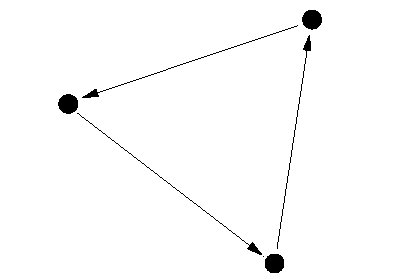
\includegraphics{./sci-pap-roc.pdf}%
\end{picture}%
\setlength{\unitlength}{3947sp}%
%
\begingroup\makeatletter\ifx\SetFigFont\undefined%
\gdef\SetFigFont#1#2#3#4#5{%
  \reset@font\fontsize{#1}{#2pt}%
  \fontfamily{#3}\fontseries{#4}\fontshape{#5}%
  \selectfont}%
\fi\endgroup%
\begin{picture}(3345,2223)(3054,-2286)
\put(5469,-1199){\makebox(0,0)[lb]{\smash{{\SetFigFont{12}{14.4}{\familydefault}{\mddefault}{\updefault}{\color[rgb]{0,0,0}smashes}%
}}}}
\put(5723,-213){\makebox(0,0)[lb]{\smash{{\SetFigFont{12}{14.4}{\familydefault}{\mddefault}{\updefault}{\color[rgb]{0,0,0}scissors}%
}}}}
\put(5381,-2271){\makebox(0,0)[lb]{\smash{{\SetFigFont{12}{14.4}{\familydefault}{\mddefault}{\updefault}{\color[rgb]{0,0,0}rock}%
}}}}
\put(3956,-1652){\makebox(0,0)[lb]{\smash{{\SetFigFont{12}{14.4}{\familydefault}{\mddefault}{\updefault}{\color[rgb]{0,0,0}covers}%
}}}}
\put(4423,-463){\makebox(0,0)[lb]{\smash{{\SetFigFont{12}{14.4}{\familydefault}{\mddefault}{\updefault}{\color[rgb]{0,0,0}cuts}%
}}}}
\put(3069,-837){\makebox(0,0)[lb]{\smash{{\SetFigFont{12}{14.4}{\familydefault}{\mddefault}{\updefault}{\color[rgb]{0,0,0}paper}%
}}}}
\end{picture}%

\end{center}
  
\hint{If at first you don't succeed\ldots \newline
try googling ``scissor paper rock lizard spock.''}

\wbvfill

\workbookpagebreak

\end{enumerate}




%\newpage
%\renewcommand{\bibname}{References for chapter 3}
%\bibliographystyle{plain}
%\bibliography{main}

%% Emacs customization
%% 
%% Local Variables: ***
%% TeX-master: "GIAM.tex" ***
%% comment-column:0 ***
%% comment-start: "%% "  ***
%% comment-end:"***" ***
%% End: ***
 

 
\chapter{Sets}

{\em No more turkey, but I'd like some more of the bread it ate. --Hank Ketcham}


\section{Basic notions of set theory}
\label{sec:basic_set_notions}

In modern mathematics there is an area called \index{Category theory} 
Category theory\footnote{The classic text by Saunders Mac Lane \cite{macl} %
is still considered one of the best introductions to Category theory.} 
which studies the 
relationships between different areas of mathematics.  More precisely,
the founders of category theory noticed that essentially the same theorems 
and proofs could be found in many different mathematical fields -- with
only the names of the structures involved changed.  In this sort of
situation one can make what is known as a \emph{categorical} argument
in which one proves the desired result in the abstract, without reference
to the details of any particular field.  In effect this allows one
to prove many theorems at once -- all you need to convert an abstract
categorical proof into a concrete one relevant to a particular area
is a sort of key or lexicon to provide the correct names for things.
Now, category theory probably shouldn't really be studied until you 
have a background that includes enough different fields that you can
make sense of their categorical correspondences.  Also, there are 
a good many mathematicians who deride category theory as 
``abstract nonsense.''   But, as someone interested in developing a facility
with proofs, you should be on the lookout for categorical correspondences.
If you ever hear yourself utter something like ``well, the proof of 
\emph{that} goes just like the proof of the 
(insert weird technical-sounding name here) theorem'' you are  
probably noticing a categorical correspondence.  

Okay, so category theory won't be of much
use to you until much later in your mathematical career (if at all), and 
one could argue that it doesn't really save that much effort.  Why not just do two or three different 
proofs instead of learning a whole new field so we can combine 
them into one?  Nevertheless, category theory is being
mentioned here at the beginning of the chapter on sets.  Why? 

We are about to see our first example of a categorical correspondence.
Logic and Set theory are different aspects of the same thing.  To
describe a set people often quote 
\index{G\"{o}del, Kurt} Kurt G\"{o}del -- 
``A set is a Many that allows itself to be thought of as a One.''  (Note
how the attempt at defining what is really an elemental, undefinable
concept ends up sounding rather mystical.)  A more practical approach is
to think of a set as the collection of things that make some open sentence
\emph{true}.\footnote{This may sound less metaphysical,
but this statement is also faulty because it defines ``set'' in terms of ``collection'' -- which will of course be defined elsewhere as ``the sort of things of which sets are one example.''} 

Recall that in Logic the atomic concepts were ``true'', ``false'', 
``sentence'' and ``statement.''    In Set theory, they are ``set'', 
``element'' and ``membership.''  These concepts (more or less) correspond to
one another.  In most books, a set is denoted either using the letter $M$ 
(which stands for the German word ``menge'') or early alphabet capital roman 
letters --
$A$, $B$, $C$, \emph{et cetera}.  Here, we will often emphasize the connection between
sets and open sentences in Logic by using a subscript notation.  The set that
corresponds to the open sentence $P(x)$ will be denoted $S_P$, we call
$S_P$ the \index{truth set} \emph{truth set} of~$P(x)$. 

\[ S_P = \{ x \suchthat P(x) \} \]


On the other hand, when we have a set given in the absence of any open 
sentence, we'll be happy to use the early alphabet, capital roman letters 
convention -- or frankly, any other letters we feel like!
Whenever we have a set $A$ given, it is easy to state a logical 
open sentence that would correspond to it.  The membership question: $M_A(x) =
\,$ ``Is $x$ in the set $A$?''  Or, more succinctly, 
$M_A(x) = \,$ ``$x \in A$''.   Thus the atomic concept ``true'' from Logic
corresponds to the answer ``yes'' to the membership question in Set theory
(and of course ``false'' corresponds to ``no'').

There are many interesting foundational issues which we are going to
sidestep in our current development of Set theory.  For instance,
recall that in Logic we always worked inside some 
\index{universe of discourse}``universe of discourse.''
As a consequence of the approach we are taking now, all of our set theoretic
work will be done within some unknown 
\index{universal set}``universal'' set.  Attempts at 
specifying (\emph{a priori}) a universal set for doing mathematics within 
are doomed to failure.  In the early days of the twentieth century
they attempted to at least get Set theory itself on a firm footing by
defining the universal set to be ``the set of all sets'' -- an innocuous
sounding idea that had funny consequences (we'll investigate this in 
Section~\ref{sec:russell}).  

In Logic we had ``sentences'' and ``statements,'' the latter were 
distinguished as having definite truth values.  The corresponding
thing in Set theory is that sets have the property that we can always
tell whether a given object is or is not in them.  If it ever becomes
necessary to talk about ``sets'' where we're not really sure what's in
them we'll use the term \emph{collection}.
  
You should think of a set as being an \emph{unordered} collection of 
things, thus $\{ \mbox{popover}, 1, \mbox{froggy} \}$ and  
$\{ 1, \mbox{froggy}, \mbox{popover} \}$ are two ways to represent the 
same set.  Also, a set either contains, or doesn't contain, a given element.
It doesn't make sense to have an element in a set multiple times.  By
convention, if an element is listed more than once when a set is
listed  we ignore the repetitions.  So, the sets
$\{ 1, 1\}$ and $\{1\}$ are really the same thing.  If the notion
of a set containing multiple instances of its elements is needed there
is a concept known as a 
\index{multiset}\emph{multiset} that is studied in Combinatorics.
In a multiset, each element is preceded by a so-called 
\index{repetition number}\emph{repetition number}
which may be the special symbol $\infty$ (indicating an unlimited number
of repetitions).  The multiset concept is useful when studying puzzles like
``How many ways can the letters of MISSISSIPPI be rearranged?'' because the
letters in MISSISSIPPI can be expressed as the multiset $\{1\cdot M, 4\cdot I,
2\cdot P, 4\cdot S \}$.  With the exception of the following exercise, in the
remainder of this chapter we will only be concerned with sets, never multisets.

\begin{exer}
(Not for the timid!) How many ways can the letters of MISSISSIPPI be arranged?
\end{exer}

If a computer scientist were seeking a data structure to implement the
notion of ``set,'' he'd want a sorted list where repetitions of an entry
were somehow disallowed.  We've already noted that a set should be thought of
as an unordered collection, and yet it's been asserted that a \emph{sorted}
list would be the right vehicle for representing a set on a computer.  Why?
One reason is that we'd like to be able to tell (quickly) whether two sets
are the same or not.  If the elements have been presorted it's easier.

Consider the difficulty in deciding whether the following two sets are
equal.

\vfill

\[ S_1 = \{ \spadesuit, 1, e, \pi, \diamondsuit, A, \Omega, h, \oplus, \epsilon \} \]

\vfill

\[ S_2 = \{ A, 1, \epsilon, \pi, e, s, \oplus,  \spadesuit, \Omega, \diamondsuit \} \]

\newpage
If instead we compare them after they've been sorted, the job is much easier.

\[ S_1 = \{1, A, \diamondsuit, e, \epsilon, h, \Omega, \oplus, \pi, \spadesuit \} \]

\[ S_2 = \{1, A, \diamondsuit, e, \epsilon, \Omega, \oplus, \pi, s, \spadesuit \} \]

This business about ordered versus unordered comes up fairly often so it's 
worth investing a few moments to figure out how it works.  If a collection
of things that is inherently unordered is handed to us we generally \emph{put}
them in an order that is pleasing to us.  Consider receiving five cards
from the dealer in a card game, or extracting seven letters from the bag 
in a game of Scrabble.  If, on the other hand, we receive 
a collection where order
is important we certainly \emph{may not} rearrange them.  Imagine someone
receiving the telephone number of an attractive other but writing it down
with the digits sorted in increasing order!  

\begin{exer}
Consider a universe consisting of just the first 5 natural numbers
$U = \{ 1, 2, 3, 4, 5 \}$.  How many different sets having 4 elements
are there in this universe?  How many different ordered collections of 4 
elements are there? 
\end{exer}

The last exercise suggests an interesting question.  If you have 
a universal set of some fixed (finite) size, how many different sets
are there?  Obviously you can't have any more elements in a set than
are in your universe.  What's the smallest possible size for a set?
Many people would answer 1 -- which isn't unreasonable! -- after all
a set is supposed to be a collection of things, and is it really possible
to have a \emph{collection} with nothing in it?  The standard answer is
0 however, mostly because it makes a certain counting formula work out
nicely.  A set with one element is known as a 
\index{singleton set}\emph{singleton set} 
(note the use of the indefinite article).  A set with no elements
is known as the 
\index{empty set}\emph{empty set} (note the definite article).  There
are as many singletons as there are elements in your universe.  They
aren't the same though, for example $1 \neq \{ 1 \}$.  There is 
only one empty set and it is denoted $\emptyset$ -- irrespective of the
universe we are working in.

Let's have a look at a small example.  Suppose we have a universal set
with 3 elements, without loss of generality, $\{1, 2, 3\}$.  It's 
possible to construct a set, whose elements are all the possible sets
in this universe.  This set is known as the 
\index{power set}\emph{power set} of the universal
set.  Indeed, we can construct the power set of \emph{any} set $A$ and
we denote it with the symbol ${\mathcal P}(A)$.  Returning to our
example we have 

\begin{center}
\begin{tabular}{rcl}
 ${\mathcal P}(\{1, 2, 3 \}) = $ & $\left\{ \rule{0pt}{10pt}  \right.$ & $\emptyset,$ \\
  & & $\{ 1 \},  \{ 2 \},  \{ 3 \},$ \\
  & & $\{ 1, 2 \},  \{ 1, 3 \},  \{ 2, 3 \},$ \\
  & & $\left.   \{ 1, 2, 3 \} \rule{0pt}{10pt} \right\}.$
\end{tabular}
\end{center}

\begin{exer} \rule{0pt}{0pt}

Find the power sets $ {\mathcal P}(\{1, 2 \})$ and 
${\mathcal P}(\{1, 2, 3, 4 \})$.  

Conjecture a formula for the number 
of elements (these are, of course, \emph{sets}) in 
${\mathcal P}(\{1, 2, \ldots n \})$.

Hint: If your conjectured formula is correct you should see 
why these sets are named as they are. 

\end{exer}

One last thing before we end this section.  The size (a.k.a. \index{cardinality}cardinality) of a set is just the number of elements in it.  We use the
very same symbol for cardinality as we do for the absolute value of a
numerical entity.  There should really never be any confusion.  If $A$ is
a set then $|A|$ means that we should count how many things are in $A$.
If $A$ isn't a set then we are talking about the ordinary absolute value

\clearpage 

\noindent{\large \bf Exercises --- \thesection\ }

\begin{enumerate}
\item What is the power set of $\emptyset$?  Hint: if you got the last exercise
in the chapter you'd know that this power set has $2^0 = 1$ element.

\hint{The power set of a set always includes the empty set as well as the whole set that we
are forming the power set of.  In this case they happen to coincide so ${\mathcal P}(\emptyset) = \{ \emptyset \}$.  Notice that $2^0 =1$.}

\item Try iterating the power set operator.  What is ${\mathcal P}({\mathcal P}(\emptyset))$?  What is ${\mathcal P}({\mathcal P}({\mathcal P}(\emptyset)))$?

\hint{I won't spoil you're fun, but as a check ${\mathcal P}({\mathcal P}(\emptyset))$ should have $2$ elements, and ${\mathcal P}({\mathcal P}({\mathcal P}(\emptyset)))$ should have $4$.}

\item Determine the following cardinalities.
  \begin{enumerate}
    \item $A = \{ 1, 2, \{3, 4, 5\}\} \quad |A| = $\rule{36pt}{1pt}
    \item $B = \{ \{1, 2, 3, 4, 5\} \} \quad |B| = $\rule{36pt}{1pt}  
  \end{enumerate}

\hint{Three and one}

\item What, in Logic, corresponds the notion $\emptyset$ in Set theory?

\hint{A contradiction.}

\item What, in Set theory, corresponds to the notion $t$ (a tautology) in Logic?

\hint{The universe of discourse.}

\item What is the truth set of the proposition $P(x) = $ ``3 divides $x$ and 2 divides $x$''?

\hint{ The set of all multiples of $6$.}

\item Find a logical open sentence such that $\{0, 1, 4, 9, \ldots \}$ is
its truth set.

\hint{Many answers are possible.  Perhaps the easiest is $\exists y \in \Integers, x = y^2$.}

\item How many singleton sets are there in the power set of 
$\{a,b,c,d,e\}$?  ``Doubleton'' sets?

\hint{5, 10}

\item How many 8 element subsets are there in
\[ {\mathcal P}(\{a,b,c,d,e,f,g,h,i,j,k,l,m,n,o,p\})? \]

\hint{ $\binom{16}{8} = 12870$}

\item How many singleton sets are there in the power set of 
$\{1,2,3, \ldots n\}$?

\hint{$n$}

\end{enumerate}



%% Emacs customization
%% 
%% Local Variables: ***
%% TeX-master: "GIAM-hw.tex" ***
%% comment-column:0 ***
%% comment-start: "%% "  ***
%% comment-end:"***" ***
%% End: ***



\newpage

\section{Containment}

There are two notions of being ``inside'' a set.  A thing may be
an \emph{element} of a set, or may be contained as
a subset.  Distinguishing these two notions of inclusion is essential.   
One difficulty that sometimes complicates things is that  a set may contain
other sets \emph{as elements}.  For instance, as we saw in the previous 
section, the elements of a power set are themselves sets.  

A set $A$ is a \index{subset}\emph{subset} of another set $B$ if all of $A$'s elements
are also in $B$.  The terminology 
\index{superset}\emph{superset} is used to refer
to $B$ in this situation, as in ``The set of all real-valued functions %
in one real variable is a superset of the polynomial functions.''  The 
subset/superset relationship is indicated with a symbol that should be
thought of as a stylized version of the less-than-or-equal sign, when
$A$ is a subset of $B$ we write $A \subseteq B$.  

We say that $A$ is 
a \index{proper subset}\emph{proper subset} of $B$ if $B$ has some elements that aren't in
$A$, and in this situation we write $A \subset B$ or if we really want
to emphasize the fact that the sets are not equal we can write 
$A \subsetneq B$.  By the way, if you want to emphasize the superset
relationship, all of these symbols can be turned around.  So for example
$A \supseteq B$ means that $A$ is a superset of $B$ although they could
potentially be equal.

As we've seen earlier, the symbol $\in$ is used between an element of
a set and the set that it's in.  The following exercise is intended to
clarify the distinction between $\in$ and $\subseteq$.

\begin{exer}
Let $A = \left\{ \rule{0pt}{10pt} 1, 2, \{ 1 \}, \{ a, b \} \right\}$.
Which of the following are true?

\vfill

\rule{72pt}{0pt} \begin{tabular}{ll}
i) $ \{ a, b \} \subseteq A$. \rule{36pt}{0pt} & vi) $  \{ 1 \} \subseteq A$.\\
ii) $ \{ a, b \} \in A$. & vii) $  \{ 1 \} \in A$.\\
iii) $  a \in A$. & viii) $  \{ 2 \} \in A$.\\
iv) $  1 \in A$. & ix) $  \{ 2 \} \subseteq A$.\\
v) $  1 \subseteq A$. & x) $  \{\{1\}\} \subseteq A$.\\
\end{tabular}
\end{exer}

\newpage

Another perspective that may help clear up the distinction between
$\in$ and $\subseteq$ is to consider what they correspond to in Logic.
The ``element of'' symbol $\in$ is used to construct open sentences
that embody the membership question -- thus it corresponds to single
sentences in Logic.  The ``set containment'' symbol $\subseteq$ goes
between two \emph{sets} and so whatever it corresponds to in Logic
should be something that can appropriately be inserted between two
sentences. Let's run through a short example to figure out what that
might be.   To keep things
simple we'll work inside the universal set $U=\{ 1, 2, 3, \ldots 50 \}$.
Let $T$ be the subset of $U$ consisting of those numbers that are 
divisible by 10, and let $F$ be those that are divisible by 5.

\[ T = \{10, 20, 30, 40, 50 \} \]
\[ F = \{5, 10, 15, 20, 25, 30, 35, 40, 45, 50 \} \]

Hopefully it is clear that $\subseteq$ can be inserted between these two sets
like so: $T \subseteq F$.  
On the other hand we can re-express the sets $T$ and $F$ using set-builder
notation in order to see clearly what their membership questions are.

\[ T = \{ x \in U \; \suchthat \; 10\divides x \} \]
\[ F = \{ x \in U \; \suchthat \; 5\divides x \} \]

What logical operator fits nicely between $10\divides x$ and $5\divides x$?
Well, of course, it's the implication arrow.  It's easy to
verify that $10\divides x \, \implies \, 5\divides x$, and it's equally easy
to note that the other direction doesn't work, $5\divides x \, \nRightarrow \, 10\divides x$ --- for instance, $5$ goes evenly into $15$, but $10$ doesn't.
 
The general statement is: if $A$ and $B$ are sets, and $M_A(x)$ and $M_B(x)$ 
are their respective membership questions, then $A \subseteq B$ corresponds
precisely to $\forall x \in U, M_A(x) \implies M_B(x)$.

    
Now to many people (me included!) this looks funny at first, $\subseteq$
in Set theory corresponds to $\implies$ in Logic.  It seems like both
of these symbols are arrows of a sort -- but they point in opposite
directions!  Personally, I resolve the apparent discrepancy by thinking
about the ``strength'' of logical predicates.  One predicate is stronger
than another if it puts more conditions on the elements that would make
it true.  For example, ``$x$ is doubly-even'' is stronger than 
``$x$ is (merely) even.''   Now, the stronger statement implies the weaker
(assuming of course that they are stronger and weaker versions of the 
same idea).  If a number is doubly-even (i.e. divisible by 4) then it
is certainly even -- but the converse is certainly not true, $6$ is even
but \emph{not} doubly-even.  Think of all this in terms of sets now.
Which set contains the other, the set of doubly-even numbers or the set
of even numbers?   Clearly the set that corresponds to more stringent
membership criteria is smaller than the set that corresponds
to less restrictive criteria, thus the set defined by a weak membership
criterion contains the one having a stronger criterion.  

If we are asked to prove that one set is contained in another as a subset,
$A \subseteq B$, there are two ways to proceed.  We may either argue by
thinking about elements, or (although this amounts to the same thing) 
we can show that $A$'s membership criterion
implies $B$'s membership criterion.

\begin{exer}
Consider $S$, the set of perfect squares and $F$, the set of perfect fourth
powers.  Which is contained in the other?  Can you prove it?
\end{exer}

We'll end this section with a fairly elementary proof -- mainly just to
illustrate how one should proceed in proving that one  set is contained in
another.

Let $D$ represent the set of all integers that are divisible by 9,

\[ D = \{ x \in \Integers \suchthat \exists k \in \Integers, \; x=9k \}. \]

Let $C$ represent the set of all integers that are divisible by 3,

\[ C = \{ x \in \Integers \suchthat \exists k \in \Integers, \; x=3k \}. \]
 
The set $D$ is contained in $C$.  Let's prove
it!

\begin{proof}
Suppose that $x$ is an arbitrary element of $D$.  From the definition
of $D$ it follows that there is an integer $k$ such that $x=9k$.  
We want to show that $x \in C$, but since $x=9k$ it is easy to 
see that $x = 3(3k)$ which shows (since $3k$ is clearly an integer)
that $x$ is in $C$.
\end{proof}

\clearpage 

\noindent{\large \bf Exercises --- \thesection\ }

\begin{enumerate}
\item Insert either $\in$ or $\subseteq$ in the blanks in the following 
sentences (in order to produce true sentences).


\begin{tabular}{lcl}
\rule{0pt}{16pt}i) $1$ \underline{\rule{36pt}{0pt}} $\{3, 2, 1, \{a, b\}\}$ & \rule{36pt}{0pt} & iii) $\{a, b\}$  \underline{\rule{36pt}{0pt}} $\{3, 2, 1, \{a, b\}\}$ \\
\rule{0pt}{16pt}ii) $\{a\}$ \underline{\rule{36pt}{0pt}} $\{a, \{a, b\}\}$ & &
iv) $\{\{a, b\}\}$  \underline{\rule{36pt}{0pt}} $\{a, \{a, b\}\}$ \\
\end{tabular}

\hint{$\in$, $\subseteq$, $\in$, $\subseteq$}

\item  Suppose that $p$ is a prime, for each $n$ in $\Integers^+$, 
define the set $P_n = \{ x \in \Integers^+ \suchthat \, p^n \divides x \}$.  
Conjecture and prove a statement about the containments between these sets.

\hint{When $p=2$ we have seen these sets.  $P_1$ is the even numbers, $P_2$ is the doubly-even numbers,
etc.}

\wbvfill

\item  Provide a counterexample to dispel the notion that a subset must
have fewer elements than its superset.

\hint{A subset is called {\em proper} if it is neither empty nor equal to the superset.   If
we are talking about finite sets then the proper subsets do indeed have fewer elements
than the supersets.  Among infinite sets it is possible to have proper subsets having the same 
number of elements as their superset, for example there are just as many even natural numbers
as there are natural numbers all told.}

\wbvfill

\workbookpagebreak

\item  We have seen that $A \subseteq B$ corresponds to $M_A \implies M_B$.
What corresponds to the contrapositive statement?

\hint{Turn ``logical negation'' into ``set complement'' and reverse the direction of the inclusion.}
 
\wbvfill

\item Determine two sets $A$ and $B$ such that both of the sentences
$A \in B$ and $A \subseteq B$ are true.

\hint{The smallest example I can think of would be $A=\emptyset$ and $B=\{\emptyset\}$.  You should come up with a different example.}

\wbvfill

\item Prove that the set of perfect fourth powers is contained in the
set of perfect squares.

\hint{It would probably be helpful to have precise definitions of the sets described in the problem.

The fourth powers are
\[ F = \{x \suchthat \exists y \in \Integers, x=y^4 \}. \]

The squares are 
\[ S = \{x \suchthat \exists z \in \Integers, x=z^2 \}. \]

To show that one set is contained in another, we need to show that the first set's membership
criterion implies that of the second set.}

\wbvfill

\end{enumerate}



%% Emacs customization
%% 
%% Local Variables: ***
%% TeX-master: "GIAM-hw.tex" ***
%% comment-column:0 ***
%% comment-start: "%% "  ***
%% comment-end:"***" ***
%% End: ***



\newpage

\section{Set operations}

In this section we'll continue to develop the correspondence between 
Logic and Set theory.

The logical connectors $\land$ and $\lor$ correspond to the set-theoretic
notions of 
\index{union}union ($\cup$) and 
\index{intersection}intersection ($\cap$).   The symbols are 
designed to provide a mnemonic for the correspondence; the Set theory
symbols are just rounded versions of those from Logic.

Explicitly, if $P(x)$ and $Q(x)$ are open sentences, then
the \emph{union} of the corresponding truth sets $S_P$ and $S_Q$
is defined by 

\[ S_P \cup S_Q \; = \{ x \in U \suchthat P(x) \lor Q(x) \}. \]

\begin{exer}
Suppose two sets $A$ and $B$ are given.  Re-express the previous
definition of ``union'' using their membership criteria, $M_A(x) =$
``$x \in A$'' and $M_B(x) = $ ``$x \in B$.''
\end{exer}

The union of more than two sets can be expressed using a big union
symbol.  For example, consider the family of real intervals defined
by $I_n = (n,n+1]$.\footnote{The elements %
of $I_n$ can also be distinguished as the solution sets of %
the inequalities $n < x \leq n+1$.}    
There's an interval for every integer $n$.  Also, every real number is in
one of these intervals.  The previous sentence can be expressed as

\[ \Reals \; = \; \bigcup_{n\in\Integers} I_n. \]

The intersection of two sets is conceptualized as ``what they have in common''
but the precise definition is found by considering conjunctions,  

\[ A \cap B \; = \; \{ x \in U \suchthat x \in A \; \land \; x \in B \}. \]

\begin{exer} 
With reference to two open sentences $P(x)$ and $Q(x)$, define the
intersection of their truth sets, $S_P \cap S_Q$.
\end{exer}

There is also a ``big'' version of the intersection symbol.  Using 
the same family of intervals as before, 

\[ \mbox{\raisebox{-2pt}{$\emptyset$}} \; = \; \bigcap_{n\in\Integers} I_n. \]

Of course the intersection of any distinct pair of these intervals is empty
so the statement above isn't particularly strong.

Negation in Logic corresponds to 
complementation in Set theory.  The 
\index{complement}\emph{complement} of a set $A$ is usually denoted by $\overline{A}$ 
(although some prefer a superscript $c$ -- as in $A^c$), this is the set
of all things that \emph{aren't} in $A$.  In thinking about complementation
one quickly sees why the importance of working within a well-defined
universal set is stressed.  Consider the set of all math textbooks.
Obviously the complement of this set would contain texts in English,
Engineering and Evolution -- but that statement is implicitly 
assuming that the universe of discourse is ``textbooks.''   It's equally
valid to say that a very long sequence of zeros and ones, a luscious 
red strawberry, and the number $\sqrt{\pi}$ 
are not math textbooks and so
these things are all elements of the complement of the set of all math
textbooks.  What is really a concern for us is the issue of whether or not
the complement of a set is well-defined, that is, can we tell for sure
whether a given item is or is not in the complement of a set.  This 
question is decidable exactly when the membership question for the
original set is decidable.   Many people think that the main
reason for working within a fixed universal set is that we then 
have well-defined complements.  The real reason that we accept
this restriction is to ensure that both membership criteria,
$M_A(x)$ and $M_{\overline{A}}(x)$, are decidable open sentences.
As an example of the sort of strangeness that can crop up, consider that
during the time that I, as the author of this book, was writing the 
last paragraph, this text was nothing more than a very long
sequence of zeros and ones in the memory of my computer\ldots

Every rule that we learned in Chapter~\ref{ch:logic} 
(see Table~\ref{tab:bool_equiv}) has a set-theoretic equivalent.  
These set-theoretic versions are
expressed using equalities (i.e. the symbol $=$ in between two sets) which
is actually a little bit funny if you think about it.  We normally
use $=$ to mean that two numbers or variables have the same numerical
magnitude, as in $12^2 = 144$, we are doing something altogether
different when we use that symbol between two sets, as in $\{1,2,3\}=
\{\sqrt{1},\sqrt{4},\sqrt{9}\}$, but people seem to be used to this
so there's no sense in quibbling.

\begin{exer}
Develop a useful definition for set equality.  In other words,
come up with a (quantified) logical statement that means the
same thing as ``$A = B$'' for two arbitrary sets $A$ and $B$.
\end{exer}

\begin{exer}
What symbol in Logic should go between the membership criteria
$M_A(x)$ and $M_B(x)$ if $A$ and $B$ are equal sets? 
\end{exer}

In Table~\ref{tab:set_equiv} the rules governing the interactions 
between the set theoretic operations are collected.
 
We are now in a position somewhat similar to when we jumped from
proving logical assertions with truth tables to doing two-column
proofs.  We have two different approaches for showing that two
sets are equal.  We can do a so-called ``element chasing'' proof
(to show $A=B$, assume $x \in A$ and prove $x \in B$ and then vice versa).
Or, we can construct a proof using the basic set equalities given
in Table~\ref{tab:set_equiv}.  Often the latter can take the form
of a two-column proof.

\begin{table}[hbt] 
\begin{center}
\begin{tabular}{c|c|c} 
 & \begin{minipage}{.35\textwidth} \centerline{Intersection}
\centerline{\rule[-10pt]{0pt}{10pt}version} \end{minipage} & 
\begin{minipage}{.35\textwidth} \centerline{Union}
\centerline{\rule[-10pt]{0pt}{10pt}version} \end{minipage} \\ \hline
\begin{minipage}{.25\textwidth} \rule{0pt}{22pt}Commutative \\ \rule{12pt}{0pt} laws\rule[-10pt]{0pt}{10pt} \end{minipage} & 
\begin{minipage}{.35\textwidth} \centerline{$A \cap B = B \cap A$} \end{minipage} & 
\begin{minipage}{.35\textwidth} \centerline{$A \cup B = B \cup A$} \end{minipage} \\ \hline
\begin{minipage}{.25\textwidth} \rule{0pt}{22pt}Associative \\ \rule{12pt}{0pt} laws\rule[-10pt]{0pt}{10pt} \end{minipage} & 
\begin{minipage}{.35\textwidth} \centerline{$A \cap (B \cap C)$\rule{26pt}{0pt}} 
\centerline{\rule{26pt}{0pt} $= (A \cap B) \cap C $}\end{minipage} &
\begin{minipage}{.35\textwidth} \centerline{$A \cup (B \cup C)$ \rule{26pt}{0pt}}
\centerline{\rule{26pt}{0pt} $= (A \cup B) \cup C $} \end{minipage} \\ \hline 
\begin{minipage}{.25\textwidth} \rule{0pt}{22pt}Distributive \\ \rule{12pt}{0pt} laws\rule[-10pt]{0pt}{10pt} \end{minipage} &  
\begin{minipage}{.35\textwidth} 
\centerline{$A \cap (B \cup C) = $ \rule{26pt}{0pt}} 
\centerline{\rule{16pt}{0pt}$(A \cap B) \cup (A \cap C)$} \end{minipage} & 
\begin{minipage}{.35\textwidth} \centerline{$A \cup (B \cap C) = $ \rule{26pt}{0pt}} 
\centerline{\rule{16pt}{0pt}$(A \cup B) \cap (A \cup C)$} \end{minipage} \\ \hline 
\begin{minipage}{.25\textwidth} \rule{0pt}{22pt}DeMorgan's \\ \rule{12pt}{0pt} laws\rule[-10pt]{0pt}{10pt} \end{minipage} & 
\begin{minipage}{.35\textwidth} \centerline{$\overline{A \cap B}$ \rule{25pt}{0pt}}
\centerline{ \rule{16pt}{0pt} $ = \; \overline{A} \cup \overline{B}$} \end{minipage} & 
\begin{minipage}{.35\textwidth} \centerline{$\overline{A \cup B}$\rule{25pt}{0pt}}
\centerline{ \rule{16pt}{0pt} $= \; \overline{A} \cap \overline{B}$} \end{minipage} \\ \hline 
\begin{minipage}{.25\textwidth} \rule{0pt}{22pt}Complementarity\rule[-10pt]{0pt}{10pt} \end{minipage} & 
\begin{minipage}{.35\textwidth} \centerline{$A \cap \overline{A} \; = \; \emptyset$} \end{minipage} & 
\begin{minipage}{.35\textwidth} \centerline{$A \cup \overline{A} \; = \; U$} \end{minipage} \\ \hline 
\begin{minipage}{.25\textwidth} \rule{0pt}{22pt}Identity \\ \rule{12pt}{0pt} laws\rule[-10pt]{0pt}{10pt} \end{minipage} & 
\begin{minipage}{.35\textwidth} \centerline{$A \cap U = A$} \end{minipage} & 
\begin{minipage}{.35\textwidth} \centerline{$A \cup \emptyset = A$} \end{minipage} \\ \hline 
\begin{minipage}{.25\textwidth} \rule{0pt}{22pt}Domination\rule[-10pt]{0pt}{10pt} \end{minipage} & 
\begin{minipage}{.35\textwidth}  \centerline{$A \cap \emptyset = \emptyset$} \end{minipage} & 
\begin{minipage}{.35\textwidth} \centerline{$A \cup U = U$} \end{minipage} \\ \hline
\begin{minipage}{.25\textwidth} \rule{0pt}{22pt}Idempotence\rule[-10pt]{0pt}{10pt} \end{minipage} & 
\begin{minipage}{.35\textwidth} \centerline{$A \cap A = A$} \end{minipage} & 
\begin{minipage}{.35\textwidth} \centerline{$A \cup A = A$} \end{minipage} \\ \hline
\begin{minipage}{.25\textwidth} \rule{0pt}{22pt}Absorption\rule[-10pt]{0pt}{10pt} \end{minipage} & 
\begin{minipage}{.35\textwidth} \centerline{$A \cap (A \cup B) = A$} \end{minipage} & 
\begin{minipage}{.35\textwidth} \centerline{$A \cup (A \cap B) = A$} \end{minipage} \\
\end{tabular} 
\end{center} 
\caption{Basic set theoretic equalities.}
\index{set theoretic equalities}
\label{tab:set_equiv}
\end{table}

%% Emacs customization
%% 
%% Local Variables: ***
%% TeX-master: "GIAM-hw.tex" ***
%% comment-column:0 ***
%% comment-start: "%% "  ***
%% comment-end:"***" ***
%% End: ***



\clearpage

Before we proceed much further in our study of set theory it would be a
good idea to give you an example.  We're going to prove the same assertion
in two different ways --- once via element chasing and once using the 
basic set theoretic equalities from Table~\ref{tab:set_equiv}.

The statement we'll prove is $A \cup B \; = \; A \cup (\overline{A} \cap B)$.

First, by chasing elements:

\begin{proof}
Suppose $x$ is an element of $A \cup B$.  By the definition of union we
know that 

\[ x \in A \lor x \in B. \]

The conjunctive identity law and the
fact that $x \in A \lor x \notin A$ is a tautology gives us an equivalent
logical statement:

\[ (x \in A \lor x \notin A) \land (x \in A \lor x \in B). \]

Finally, this last statement is equivalent to

\[ x \in A \lor (x \notin A \land x \in B) \]

\noindent which is the definition of $x \in A \cup (\overline{A} \cap B)$.

On the other hand, if we assume that $x \in A \cup (\overline{A} \cap B)$, it follows that 

\[ x \in A \lor (x \notin A \land x \in B). \]

Applying the distributive law, disjunctive complementarity and the identity law,
in sequence we obtain

\begin{gather*} 
 x \in A \lor (x \notin A \land x \in B) \\
\cong (x \in A \lor x \notin A) \land (x \in A \lor x \in B) \\
\cong t \land (x \in A \lor x \in B) \\
\cong x \in A \lor x \in B
\end{gather*}

The last statement in this chain of logical equivalences provides the definition of $x \in A \cup B$.

\end{proof}

A two-column proof of the same statement looks like this:

\begin{proof}

\begin{tabular}{cccl}
  & $A \cup B$ & \rule{36pt}{0pt} & Given \\
$=$ & $U \cap (A \cup B)$ & & Identity law \\
$=$ & $(A \cup \overline{A}) \cap (A \cup B)$ & & Complementarity \\
$=$ & $(A \cup (\overline{A} \cap B)$ & & Distributive law\\
\end{tabular}

\end{proof}

There are some notions within Set theory that don't have any clear
parallels in Logic.  One of these is essentially a generalization 
of the concept of ``complements.''   If you think of the set $\overline{A}$
as being the difference between the universal set $U$ and the set $A$
you are on the right track.  The 
\index{difference (of sets)}\emph{difference} between two sets is written 
$A \setminus B$ (sadly, sometimes this is denoted using the ordinary 
subtraction symbol $A-B$) and is defined by

\[   A \setminus B = A \cap \overline{B}. \]

\noindent The difference, $A \setminus B$, consists of those elements of $A$ that aren't in $B$.  In some developments of Set theory, the difference of sets is 
defined first and then complementation is defined by $\overline{A} = U \setminus A$.  

The difference of sets (like the difference of real numbers) is not a 
commutative operation.  In other words $A \setminus B \neq B \setminus A$ 
(in general).  It is possible to define an operation that acts somewhat 
like the difference, but that \emph{is} commutative.  The 
\index{symmetric difference}\emph{symmetric difference} 
of two sets is denoted using a 
triangle (really a capital Greek delta)

\[ A \triangle B = (A \setminus B) \cup (B\setminus A). \]

\begin{exer}
Show that  $A \triangle B = (A \cup B) \setminus (A \cap B)$.
\end{exer}

Come on!  You read right past that exercise without even pausing!

What?  You say you \emph{did} try it and it was too hard?

Okay, just for you (and this time only) I've prepared an aid to
help you through\ldots

On the next page is a two-column proof of the result you need to 
prove, but the lines of the proof are all scrambled.
Make a copy and cut out all the pieces and then glue them together
into a valid proof.

So, no more excuses, just do it!

\newpage




\begin{tabular}{|c|l|}\hline
\rule[-16pt]{0pt}{44pt}$= (A \cap \overline{B}) \cup (B \cap \overline{A})$ & \rule{12pt}{0pt} identity law \\\hline
\rule[-16pt]{0pt}{44pt}$= (A \cup B) \cap \overline{(A \cap B)}$ & \rule{12pt}{0pt} def. of relative difference \rule{12pt}{0pt} \\\hline
\rule[-16pt]{0pt}{44pt}$(A \cup B) \setminus (A \cap B)$ & \rule{12pt}{0pt} Given  \\\hline
\rule[-16pt]{0pt}{44pt}\rule{12pt}{0pt}$= ((A \cap \overline{A}) \cup (A \cap \overline{B})) \cup ((B \cap \overline{A}) \cup (B \cap \overline{B}))$ \rule{12pt}{0pt} & \rule{12pt}{0pt} distributive law  \\\hline
\rule[-16pt]{0pt}{44pt}$= (A \setminus B) \cup (B \setminus A)$ & \rule{12pt}{0pt}  def. of relative difference \\\hline
\rule[-16pt]{0pt}{44pt}$= (A \cap \overline{(A \cap B)}) \cup (B \cap \overline{(A \cap B)})$ & \rule{12pt}{0pt} distributive law \\\hline
\rule[-16pt]{0pt}{44pt}$= A \triangle B $ & \rule{12pt}{0pt} def. of symmetric difference \rule{12pt}{0pt}\\\hline
\rule[-16pt]{0pt}{44pt}$= (A \cap (\overline{A} \cup \overline{B}) \cup (B \cap (\overline{A} \cup \overline{B}))$ & \rule{12pt}{0pt} DeMorgan's law \\\hline
\rule[-16pt]{0pt}{44pt}$= (\emptyset \cup (A \cap \overline{B})) \cup ((B \cap \overline{A}) \cup \emptyset)$ & \rule{12pt}{0pt} complementarity \\\hline
\end{tabular}

\clearpage 

\noindent{\large \bf Exercises --- \thesection\ }

\begin{enumerate}
\item Let $A = \{1, 2, \{1, 2\}, b\}$ and let $B=\{a, b, \{1, 2\} \}$.
Find the following:
  \begin{enumerate}
  \item $A \cap B$   \hint{ $ \{ b,  \{1, 2\} \} $ }
  \item $A \cup B$ \hint{ $ \{1, 2, a, b, \{1, 2\} \} $ }
  \item $A \setminus B$ \hint{  $ \{ 1, 2 \} $ }
  \item $B \setminus A$ \hint{ $ \{ a \} $ }
  \item $A \triangle B$ \hint{ $ \{ 1, 2, a \} $ }
  \end{enumerate}

\vfill

\item In a standard deck of playing cards one can distinguish sets
based on face-value and/or suit.  Let $A, 2, \ldots 9, 10, J, Q$ and $K$
represent the sets of cards having the various face-values.  Also, let
$\heartsuit$, $\spadesuit$, $\clubsuit$ and $\diamondsuit$ be the 
sets of cards having the possible suits.  Find the following
  \begin{enumerate}
  \item $A \cap \heartsuit$ \hint{This is just the ace of hearts.}
  \item $A \cup \heartsuit$ \hint{All of the hearts and the other three aces}
  \item $J \cap (\spadesuit \cup \heartsuit)$ \hint{ These two cards are known as the one-eyed jacks.}
  \item $K \cap \heartsuit$ \hint{The king of hearts, a.k.a. the suicide king.}
  \item $A \cap K$ \hint{$\emptyset$ }
  \item $A \cup K$ \hint{Eight cards: all four kings and all four aces.}
  \end{enumerate}

\vfill

\hintspagebreak

\item Do element-chasing proofs (show that an element is in the left-hand side if and only if it is in the right-hand side) to prove each of the following set equalities.  

  \begin{enumerate}
  \item $\overline{A\cap B} \; = \; \overline{A}\cup\overline{B}$

  \item $A\cup B \; = \; A\cup(\overline{A}\cap B)$

  \item $A\triangle B \; = \; (A\cup B)\setminus(A\cap B)$

  \item $(A\cup B)\setminus C \; = \; (A\setminus C)\cup(B\setminus C)$

  \end{enumerate}

\hint{Here's the first one (although I'm omiting justifications for each step.

\begin{gather*}
x \in \overline{A\cap B} \\
\iff \; {\lnot}(x \in A\cap B) \\
\iff \; {\lnot}(x \in A \; \land \; x \in B) \\
\iff \; {\lnot}(x \in A) \; \lor \; {\lnot}(x \in B) \\
\iff \; x \in \overline{A}  \; \lor \; x \in \overline{B} \\
\iff \; x \in \overline{A} \cup \overline{B}
\end{gather*}
}



\item For each positive integer $n$, we'll define an interval $I_n$
by

\[ I_n = [-n, 1/n). \]

Find the union and intersection of all the intervals in this infinite family.

\[ \bigcup_{n \in \Naturals} I_n \quad = \]

\[ \bigcap_{n \in \Naturals} I_n \quad = \]

\hint{To better understand what is going on, first figure out what the first three or four
intervals actually are.

\[ I_1 \; = \; \underline{\rule{96pt}{0pt}} \]
\[ I_2 \; = \; \underline{\rule{96pt}{0pt}} \]
\[ I_3 \; = \; \underline{\rule{96pt}{0pt}} \]
\[ I_4 \; = \; \underline{\rule{96pt}{0pt}} \]

Any negative real number $r$ will be in the intersection only if  $r \geq -1$.  Certainly $0$ is in
the intersection since it is in each of the intervals.  Are there any positive numbers in the intersection?

In order to be in the union a real number just needs to be in {\em one} of the intervals.
}

\item There is a set $X$ such that, for all sets $A$, we have 
$X \triangle A = A$.  What is $X$?

\item There is a set $Y$ such that, for all sets $A$, we have 
$Y \triangle A = \overline{A}$.  What is $Y$?

\hint{One of the answers to the last two questions is $\emptyset$ and the other is $U$.  Decide
which is which.}

\item In proving a set-theoretic identity, we are basically showing that
two sets are equal.  One reasonable way to proceed is to show that
each is contained in the other.  Prove that 
$A \cap (B \cup C) = (A \cap B) \cup (A \cap C)$ by showing that 
$A \cap (B \cup C) \subseteq (A \cap B) \cup (A \cap C)$ and 
$(A \cap B) \cup (A \cap C) \subseteq A \cap (B \cup C)$.

\item Prove that 
$A \cup (B \cap C) = (A \cup B) \cap (A \cup C)$ by showing that 
$A \cup (B \cap C) \subseteq (A \cup B) \cap (A \cup C)$ and 
$(A \cup B) \cap (A \cup C) \subseteq A \cup (B \cap C)$.

\hint{This exercise, as well as the previous one, is really just about converting set-theoretic
statements into their logical equivalents, applying some rules of logic that we've already verified,
and then returning to a set-theoretic version of things.}
 
\item Prove the set-theoretic versions of DeMorgan's laws using the technique
discussed in the previous problems.

\item The previous technique (showing that $A=B$ by arguing that
$A \subseteq B \; \land \; B \subseteq A$) will have an outline something like

\begin{proof} 
First we will show that $A \subseteq B$.\newline
Towards that end, suppose $x \in A$.

\begin{center}
$\vdots$
\end{center}

Thus $x \in B$.

Now, we will show that $B \subseteq A$. \newline
Suppose that $x \in B$.

\begin{center}
$\vdots$
\end{center}

Thus $x \in A$.

Therefore $A \subseteq B \; \land \; B \subseteq A$ so we conclude that $A=B$.
\end{proof}

Formulate a proof that $A \triangle B \; = \; (A \cup B) \setminus (A \cap B)$.

\hint{The definition of $A \triangle B$ is $(A\setminus B) \cup (B\setminus A)$.  The definition of 
$X \setminus Y$ is $X \cap \overline{Y}$.   Restating things in terms of $\cap$ and $\cup$ (and complementation) should help.  So your first few lines should be:

 \begin{quote} 
 Suppose $x \in  A \triangle B$.  
 
Then, by definition, $x \in (A\setminus B) \cup (B\setminus A)$.
 
 So, $x \in (A \cap \overline{B}) \cup (B \cap \overline{A})$.
   
\begin{center}
$\vdots$
\end{center}

\end{quote}
}

\end{enumerate}


%% Emacs customization
%% 
%% Local Variables: ***
%% TeX-master: "GIAM-hw.tex" ***
%% comment-column:0 ***
%% comment-start: "%% "  ***
%% comment-end:"***" ***
%% End: ***



\newpage


\section{Venn diagrams}

Hopefully, you've seen 
\index{Venn diagram}Venn diagrams before, but possibly 
you haven't thought deeply about them. Venn diagrams take 
advantage of an obvious but important property of closed 
curves drawn in the plane.  They divide the points in the
plane into two sets, those that are inside the curve and
those that are outside!  (Forget for a moment about the points
that are on the curve.)  This seemingly obvious statement
is known as the 
\index{Jordan curve theorem}\emph{Jordan curve theorem}, and actually
requires some details.  A 
\index{Jordan curve}\emph{Jordan curve} is the sort 
of curve you might draw if you are required to end where
you began and you are required not to cross-over any portion 
of the curve that has already been drawn.  In technical
terms such a curve is called \emph{continuous}, \emph{simple} 
and \emph{closed}.
The Jordan curve theorem is one of those statements that hardly
seems like it needs a proof, but nevertheless, the proof of this
statement is probably the best-remembered work of the famous
French mathematician \index{Jordan, Camille}Camille Jordan.

The prototypical Venn diagram is the picture that looks something
like the view through a set of binoculars.

\vspace{.1in}

\begin{picture}(0,0)%
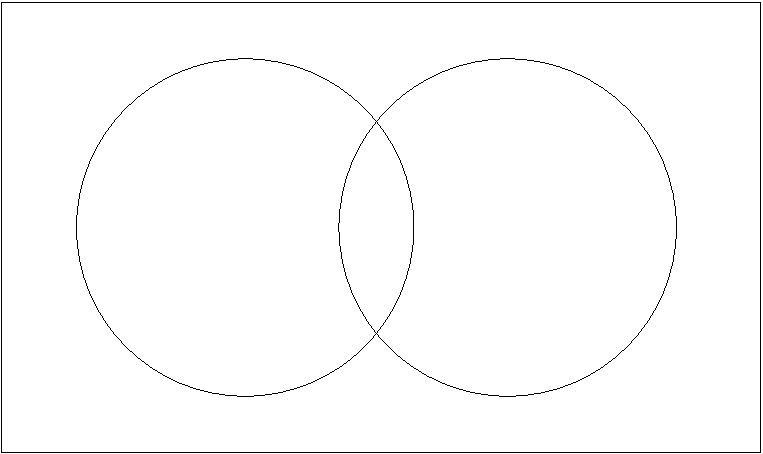
\includegraphics{figures/first_Venn.pdf}%
\end{picture}%
\setlength{\unitlength}{3947sp}%
%
\begingroup\makeatletter\ifx\SetFigFont\undefined%
\gdef\SetFigFont#1#2#3#4#5{%
  \reset@font\fontsize{#1}{#2pt}%
  \fontfamily{#3}\fontseries{#4}\fontshape{#5}%
  \selectfont}%
\fi\endgroup%
\begin{picture}(6099,3624)(1189,-3673)
\put(2326,-1036){\makebox(0,0)[lb]{\smash{{\SetFigFont{12}{14.4}{\familydefault}{\mddefault}{\updefault}{\color[rgb]{0,0,0}A}%
}}}}
\put(6001,-1036){\makebox(0,0)[lb]{\smash{{\SetFigFont{12}{14.4}{\familydefault}{\mddefault}{\updefault}{\color[rgb]{0,0,0}B}%
}}}}
\put(1276,-286){\makebox(0,0)[lb]{\smash{{\SetFigFont{12}{14.4}{\familydefault}{\mddefault}{\updefault}{\color[rgb]{0,0,0}U}%
}}}}
\end{picture}%


\vspace{.1in}

In a Venn diagram the 
\index{universe of discourse}universe of discourse is normally drawn as
a rectangular region inside of which all the action occurs.  Each
set in a Venn diagram is depicted by drawing a simple closed curve -- 
typically a circle, but not necessarily!  For instance, if you
want to draw a Venn diagram that shows all the possible intersections
among four sets, you'll find it's impossible with (only) circles.

\vspace{.1in}

\begin{picture}(0,0)%
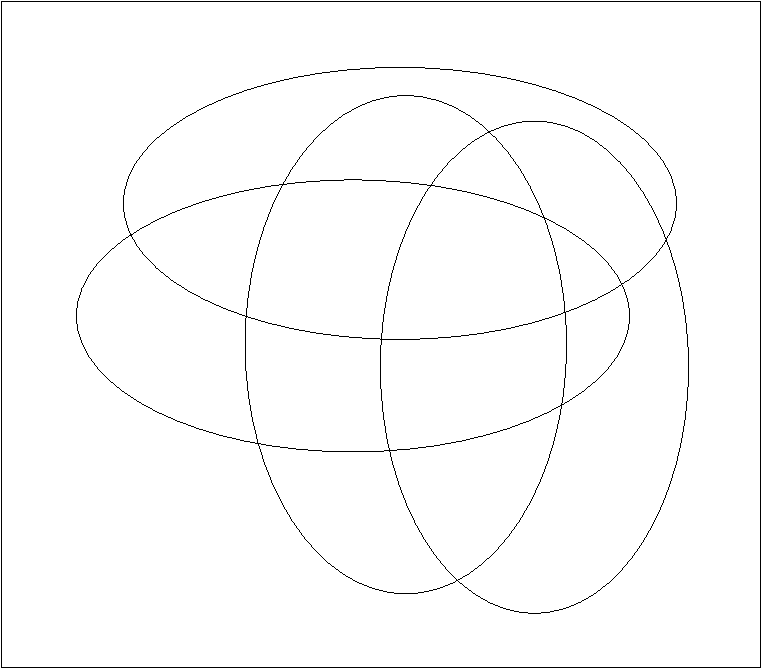
\includegraphics{figures/4set_Venn.pdf}%
\end{picture}%
\setlength{\unitlength}{3947sp}%
%
\begingroup\makeatletter\ifx\SetFigFont\undefined%
\gdef\SetFigFont#1#2#3#4#5{%
  \reset@font\fontsize{#1}{#2pt}%
  \fontfamily{#3}\fontseries{#4}\fontshape{#5}%
  \selectfont}%
\fi\endgroup%
\begin{picture}(6099,5349)(1189,-5398)
\put(1276,-286){\makebox(0,0)[lb]{\smash{{\SetFigFont{12}{14.4}{\familydefault}{\mddefault}{\updefault}{\color[rgb]{0,0,0}U}%
}}}}
\put(2551,-1261){\makebox(0,0)[lb]{\smash{{\SetFigFont{12}{14.4}{\familydefault}{\mddefault}{\updefault}{\color[rgb]{0,0,0}A}%
}}}}
\put(3976,-4636){\makebox(0,0)[lb]{\smash{{\SetFigFont{12}{14.4}{\familydefault}{\mddefault}{\updefault}{\color[rgb]{0,0,0}C}%
}}}}
\put(6001,-4561){\makebox(0,0)[lb]{\smash{{\SetFigFont{12}{14.4}{\familydefault}{\mddefault}{\updefault}{\color[rgb]{0,0,0}D}%
}}}}
\put(2026,-2911){\makebox(0,0)[lb]{\smash{{\SetFigFont{12}{14.4}{\familydefault}{\mddefault}{\updefault}{\color[rgb]{0,0,0}B}%
}}}}
\end{picture}%


\vspace{.1in}

\begin{exer}
Verify that the diagram above has regions representing all 16 possible
intersections of 4 sets.
\end{exer}

There is a certain ``zen'' to Venn diagrams that must be internalized,
but once you have done so they can be used to think very effectively
about the relationships between sets.  The main deal is that the points
inside of one of the simple closed curves are not necessarily in the set --
only \emph{some} of the points inside a simple closed curve are in the
set, and we don't know precisely where they are!  The various simple closed 
curves in a Venn diagram divide the universe up into a bunch of regions.
It might be best to think of these regions as fenced-in areas in which
the elements of a set mill about, much like domesticated animals 
in their pens.
One of our main tools in working with Venn diagrams is to deduce that
certain of these regions don't contain any elements -- we then mark that
region with the emptyset symbol ($\emptyset$). 

Here is a small example of a finite universe.

\vspace{.1in}

\begin{picture}(0,0)%
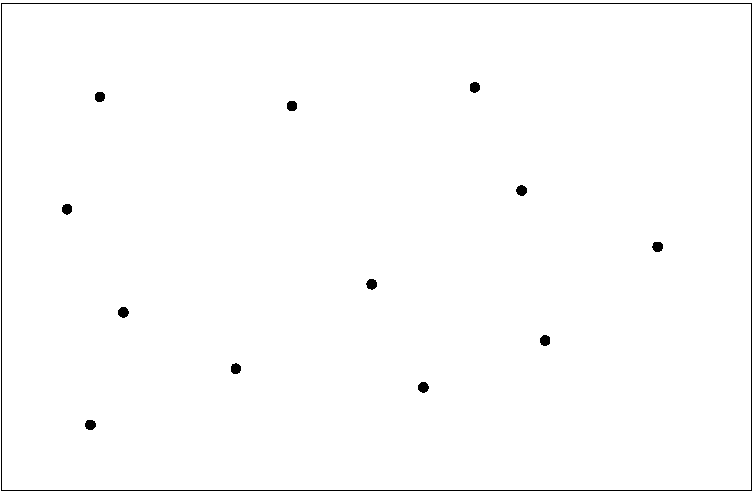
\includegraphics{figures/silly_universe.pdf}%
\end{picture}%
\setlength{\unitlength}{3947sp}%
%
\begingroup\makeatletter\ifx\SetFigFont\undefined%
\gdef\SetFigFont#1#2#3#4#5{%
  \reset@font\fontsize{#1}{#2pt}%
  \fontfamily{#3}\fontseries{#4}\fontshape{#5}%
  \selectfont}%
\fi\endgroup%
\begin{picture}(6024,3924)(1189,-4273)
\put(2101,-1036){\makebox(0,0)[lb]{\smash{{\SetFigFont{12}{14.4}{\familydefault}{\mddefault}{\updefault}{\color[rgb]{0,0,0}Mr. Ed}%
}}}}
\put(1801,-1936){\makebox(0,0)[lb]{\smash{{\SetFigFont{12}{14.4}{\familydefault}{\mddefault}{\updefault}{\color[rgb]{0,0,0}Shadowfax}%
}}}}
\put(2251,-2761){\makebox(0,0)[lb]{\smash{{\SetFigFont{12}{14.4}{\familydefault}{\mddefault}{\updefault}{\color[rgb]{0,0,0}Silver}%
}}}}
\put(2026,-3661){\makebox(0,0)[lb]{\smash{{\SetFigFont{12}{14.4}{\familydefault}{\mddefault}{\updefault}{\color[rgb]{0,0,0}Secretariat}%
}}}}
\put(3151,-3211){\makebox(0,0)[lb]{\smash{{\SetFigFont{12}{14.4}{\familydefault}{\mddefault}{\updefault}{\color[rgb]{0,0,0}Misty}%
}}}}
\put(3601,-1111){\makebox(0,0)[lb]{\smash{{\SetFigFont{12}{14.4}{\familydefault}{\mddefault}{\updefault}{\color[rgb]{0,0,0}Black Beauty}%
}}}}
\put(4201,-2536){\makebox(0,0)[lb]{\smash{{\SetFigFont{12}{14.4}{\familydefault}{\mddefault}{\updefault}{\color[rgb]{0,0,0}Heckle}%
}}}}
\put(5101,-961){\makebox(0,0)[lb]{\smash{{\SetFigFont{12}{14.4}{\familydefault}{\mddefault}{\updefault}{\color[rgb]{0,0,0}Donald Duck}%
}}}}
\put(4651,-3436){\makebox(0,0)[lb]{\smash{{\SetFigFont{12}{14.4}{\familydefault}{\mddefault}{\updefault}{\color[rgb]{0,0,0}Wile E. Coyote}%
}}}}
\put(5626,-2986){\makebox(0,0)[lb]{\smash{{\SetFigFont{12}{14.4}{\familydefault}{\mddefault}{\updefault}{\color[rgb]{0,0,0}Tweety Bird}%
}}}}
\put(6526,-2236){\makebox(0,0)[lb]{\smash{{\SetFigFont{12}{14.4}{\familydefault}{\mddefault}{\updefault}{\color[rgb]{0,0,0}Ren}%
}}}}
\put(5476,-1786){\makebox(0,0)[lb]{\smash{{\SetFigFont{12}{14.4}{\familydefault}{\mddefault}{\updefault}{\color[rgb]{0,0,0}Snowball}%
}}}}
\end{picture}%


\vspace{.1in}

\noindent And here is the same universe with some Jordan curves 
used to encircle two subsets.

\vspace{.1in}

\begin{picture}(0,0)%
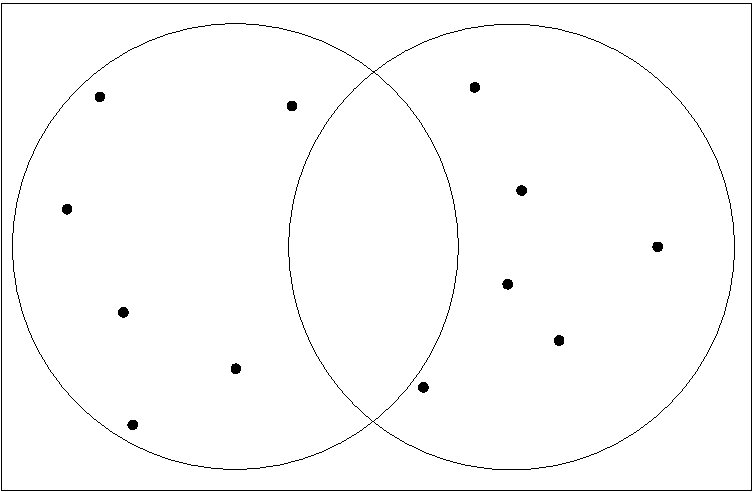
\includegraphics{./silly_w_sets.pdf}%
\end{picture}%
\setlength{\unitlength}{3947sp}%
%
\begingroup\makeatletter\ifx\SetFigFont\undefined%
\gdef\SetFigFont#1#2#3#4#5{%
  \reset@font\fontsize{#1}{#2pt}%
  \fontfamily{#3}\fontseries{#4}\fontshape{#5}%
  \selectfont}%
\fi\endgroup%
\begin{picture}(6024,3924)(1189,-4273)
\put(2101,-1036){\makebox(0,0)[lb]{\smash{{\SetFigFont{12}{14.4}{\familydefault}{\mddefault}{\updefault}{\color[rgb]{0,0,0}Mr. Ed}%
}}}}
\put(1801,-1936){\makebox(0,0)[lb]{\smash{{\SetFigFont{12}{14.4}{\familydefault}{\mddefault}{\updefault}{\color[rgb]{0,0,0}Shadowfax}%
}}}}
\put(2251,-2761){\makebox(0,0)[lb]{\smash{{\SetFigFont{12}{14.4}{\familydefault}{\mddefault}{\updefault}{\color[rgb]{0,0,0}Silver}%
}}}}
\put(3151,-3211){\makebox(0,0)[lb]{\smash{{\SetFigFont{12}{14.4}{\familydefault}{\mddefault}{\updefault}{\color[rgb]{0,0,0}Misty}%
}}}}
\put(3601,-1111){\makebox(0,0)[lb]{\smash{{\SetFigFont{12}{14.4}{\familydefault}{\mddefault}{\updefault}{\color[rgb]{0,0,0}Black Beauty}%
}}}}
\put(5101,-961){\makebox(0,0)[lb]{\smash{{\SetFigFont{12}{14.4}{\familydefault}{\mddefault}{\updefault}{\color[rgb]{0,0,0}Donald Duck}%
}}}}
\put(5326,-2536){\makebox(0,0)[lb]{\smash{{\SetFigFont{12}{14.4}{\familydefault}{\mddefault}{\updefault}{\color[rgb]{0,0,0}Heckle}%
}}}}
\put(2326,-3661){\makebox(0,0)[lb]{\smash{{\SetFigFont{12}{14.4}{\familydefault}{\mddefault}{\updefault}{\color[rgb]{0,0,0}Secretariat}%
}}}}
\put(5476,-1786){\makebox(0,0)[lb]{\smash{{\SetFigFont{12}{14.4}{\familydefault}{\mddefault}{\updefault}{\color[rgb]{0,0,0}Snowball}%
}}}}
\put(4651,-3361){\makebox(0,0)[lb]{\smash{{\SetFigFont{12}{14.4}{\familydefault}{\mddefault}{\updefault}{\color[rgb]{0,0,0}Wile E. Coyote}%
}}}}
\put(6526,-2236){\makebox(0,0)[lb]{\smash{{\SetFigFont{12}{14.4}{\familydefault}{\mddefault}{\updefault}{\color[rgb]{0,0,0}Ren}%
}}}}
\put(1501,-3511){\makebox(0,0)[lb]{\smash{{\SetFigFont{12}{14.4}{\familydefault}{\mddefault}{\updefault}{\color[rgb]{0,0,0}H}%
}}}}
\put(6601,-3661){\makebox(0,0)[lb]{\smash{{\SetFigFont{12}{14.4}{\familydefault}{\mddefault}{\updefault}{\color[rgb]{0,0,0}C}%
}}}}
\put(5701,-2986){\makebox(0,0)[lb]{\smash{{\SetFigFont{12}{14.4}{\familydefault}{\mddefault}{\updefault}{\color[rgb]{0,0,0}Tweety Bird}%
}}}}
\end{picture}%


\vspace{.1in}

This picture might lead us to think that the set of cartoon characters
and the set of horses are disjoint, so we thought it would be nice
to add one more element to our universe in order to dispel that notion.

\vspace{.1in}

\begin{picture}(0,0)%
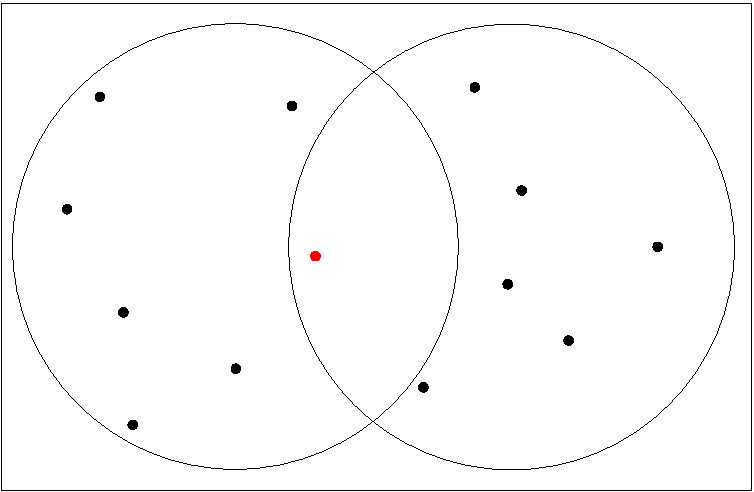
\includegraphics{./silly_w_counter_ex.pdf}%
\end{picture}%
\setlength{\unitlength}{3947sp}%
%
\begingroup\makeatletter\ifx\SetFigFont\undefined%
\gdef\SetFigFont#1#2#3#4#5{%
  \reset@font\fontsize{#1}{#2pt}%
  \fontfamily{#3}\fontseries{#4}\fontshape{#5}%
  \selectfont}%
\fi\endgroup%
\begin{picture}(6024,3924)(1189,-4273)
\put(2101,-1036){\makebox(0,0)[lb]{\smash{{\SetFigFont{12}{14.4}{\familydefault}{\mddefault}{\updefault}{\color[rgb]{0,0,0}Mr. Ed}%
}}}}
\put(1801,-1936){\makebox(0,0)[lb]{\smash{{\SetFigFont{12}{14.4}{\familydefault}{\mddefault}{\updefault}{\color[rgb]{0,0,0}Shadowfax}%
}}}}
\put(2251,-2761){\makebox(0,0)[lb]{\smash{{\SetFigFont{12}{14.4}{\familydefault}{\mddefault}{\updefault}{\color[rgb]{0,0,0}Silver}%
}}}}
\put(3151,-3211){\makebox(0,0)[lb]{\smash{{\SetFigFont{12}{14.4}{\familydefault}{\mddefault}{\updefault}{\color[rgb]{0,0,0}Misty}%
}}}}
\put(3601,-1111){\makebox(0,0)[lb]{\smash{{\SetFigFont{12}{14.4}{\familydefault}{\mddefault}{\updefault}{\color[rgb]{0,0,0}Black Beauty}%
}}}}
\put(5101,-961){\makebox(0,0)[lb]{\smash{{\SetFigFont{12}{14.4}{\familydefault}{\mddefault}{\updefault}{\color[rgb]{0,0,0}Donald Duck}%
}}}}
\put(5326,-2536){\makebox(0,0)[lb]{\smash{{\SetFigFont{12}{14.4}{\familydefault}{\mddefault}{\updefault}{\color[rgb]{0,0,0}Heckle}%
}}}}
\put(2326,-3661){\makebox(0,0)[lb]{\smash{{\SetFigFont{12}{14.4}{\familydefault}{\mddefault}{\updefault}{\color[rgb]{0,0,0}Secretariat}%
}}}}
\put(5476,-1786){\makebox(0,0)[lb]{\smash{{\SetFigFont{12}{14.4}{\familydefault}{\mddefault}{\updefault}{\color[rgb]{0,0,0}Snowball}%
}}}}
\put(4651,-3361){\makebox(0,0)[lb]{\smash{{\SetFigFont{12}{14.4}{\familydefault}{\mddefault}{\updefault}{\color[rgb]{0,0,0}Wile E. Coyote}%
}}}}
\put(6526,-2236){\makebox(0,0)[lb]{\smash{{\SetFigFont{12}{14.4}{\familydefault}{\mddefault}{\updefault}{\color[rgb]{0,0,0}Ren}%
}}}}
\put(1501,-3511){\makebox(0,0)[lb]{\smash{{\SetFigFont{12}{14.4}{\familydefault}{\mddefault}{\updefault}{\color[rgb]{0,0,0}H}%
}}}}
\put(6601,-3661){\makebox(0,0)[lb]{\smash{{\SetFigFont{12}{14.4}{\familydefault}{\mddefault}{\updefault}{\color[rgb]{0,0,0}C}%
}}}}
\put(3826,-2311){\makebox(0,0)[lb]{\smash{{\SetFigFont{12}{14.4}{\familydefault}{\mddefault}{\updefault}{\color[rgb]{1,0,0}Night Mare}%
}}}}
\put(5776,-2986){\makebox(0,0)[lb]{\smash{{\SetFigFont{12}{14.4}{\familydefault}{\mddefault}{\updefault}{\color[rgb]{0,0,0}Tweety Bird}%
}}}}
\end{picture}%


\vspace{.1in}


Suppose we have two sets $A$ and $B$ and we're interested
in proving that $B \subseteq A$.  The job is done if we can show that
all of $B$'s elements are actually in the eye-shaped region that represents
the intersection $A \cap B$.  It's equivalent if we can show that the
region marked with $\emptyset$ in the following diagram is actually empty.

\vspace{.1in}

\begin{picture}(0,0)%
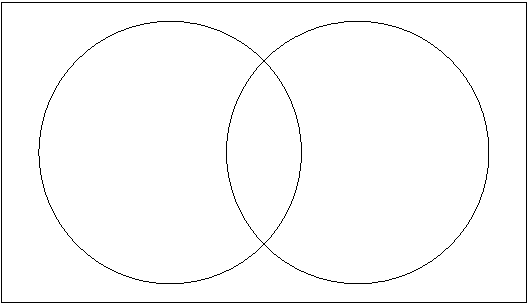
\includegraphics{./Venn_showing_implies.pdf}%
\end{picture}%
\setlength{\unitlength}{3947sp}%
%
\begingroup\makeatletter\ifx\SetFigFont\undefined%
\gdef\SetFigFont#1#2#3#4#5{%
  \reset@font\fontsize{#1}{#2pt}%
  \fontfamily{#3}\fontseries{#4}\fontshape{#5}%
  \selectfont}%
\fi\endgroup%
\begin{picture}(4224,2424)(2389,-2773)
\put(2926,-736){\makebox(0,0)[lb]{\smash{{\SetFigFont{12}{14.4}{\familydefault}{\mddefault}{\updefault}{\color[rgb]{0,0,0}A}%
}}}}
\put(6001,-736){\makebox(0,0)[lb]{\smash{{\SetFigFont{12}{14.4}{\familydefault}{\mddefault}{\updefault}{\color[rgb]{0,0,0}B}%
}}}}
\put(5251,-1561){\makebox(0,0)[lb]{\smash{{\SetFigFont{12}{14.4}{\familydefault}{\mddefault}{\updefault}{\color[rgb]{0,0,0}$\emptyset$}%
}}}}
\end{picture}%


\vspace{.1in}

Let's put all this together.  The inclusion $B \subseteq A$ corresponds
to the logical sentence $M_B \implies M_A$.  We know that implications
are equivalent to OR statements, so $M_B \implies M_A \, \cong \, 
{\lnot}M_B \lor M_A$.  The notion that the region we've 
indicated above is empty is written as $\overline{A} \cap B \, = \, \emptyset$,
in logical terms this is ${\lnot}M_A \land M_B \, \cong \, c$.  
Finally, we apply DeMorgan's law and a commutation to get 
${\lnot}M_B \lor M_A \, \cong \, t$.  You should take note of the 
convention that when you see a logical sentence just written on the 
page (as is the case with $M_B \implies M_A$ in the first sentence
of this paragraph) what's being asserted is that the sentence is 
\emph{universally true}.
Thus, writing $M_B \implies M_A$ is the same thing as writing 
$M_B \implies M_A \, \cong \, t$.

One can use information that is known \emph{a priori} when 
drawing a Venn diagram.  For instance if two sets are known 
to be disjoint, or if one is known to be contained in the other,
we can draw Venn diagrams like the following.

\vspace{.1in}

\begin{picture}(0,0)%
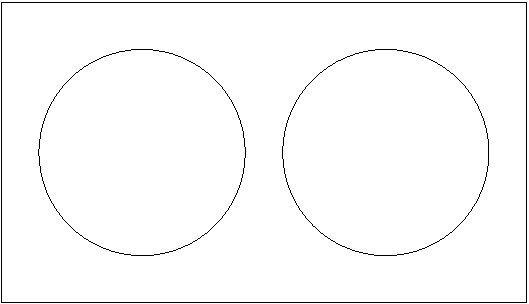
\includegraphics{figures/disjoint_Venn.pdf}%
\end{picture}%
\setlength{\unitlength}{3947sp}%
%
\begingroup\makeatletter\ifx\SetFigFont\undefined%
\gdef\SetFigFont#1#2#3#4#5{%
  \reset@font\fontsize{#1}{#2pt}%
  \fontfamily{#3}\fontseries{#4}\fontshape{#5}%
  \selectfont}%
\fi\endgroup%
\begin{picture}(4224,2424)(2389,-2773)
\put(2926,-736){\makebox(0,0)[lb]{\smash{{\SetFigFont{12}{14.4}{\familydefault}{\mddefault}{\updefault}{\color[rgb]{0,0,0}A}%
}}}}
\put(6001,-736){\makebox(0,0)[lb]{\smash{{\SetFigFont{12}{14.4}{\familydefault}{\mddefault}{\updefault}{\color[rgb]{0,0,0}B}%
}}}}
\end{picture}%


\vspace{.2in}

\begin{picture}(0,0)%
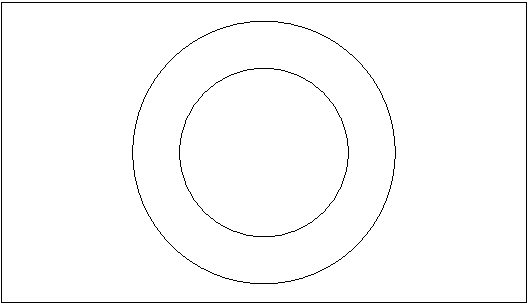
\includegraphics{figures/containment_Venn.pdf}%
\end{picture}%
\setlength{\unitlength}{3947sp}%
%
\begingroup\makeatletter\ifx\SetFigFont\undefined%
\gdef\SetFigFont#1#2#3#4#5{%
  \reset@font\fontsize{#1}{#2pt}%
  \fontfamily{#3}\fontseries{#4}\fontshape{#5}%
  \selectfont}%
\fi\endgroup%
\begin{picture}(4224,2424)(2389,-2773)
\put(3676,-736){\makebox(0,0)[lb]{\smash{{\SetFigFont{12}{14.4}{\familydefault}{\mddefault}{\updefault}{\color[rgb]{0,0,0}A}%
}}}}
\put(4726,-1186){\makebox(0,0)[lb]{\smash{{\SetFigFont{12}{14.4}{\familydefault}{\mddefault}{\updefault}{\color[rgb]{0,0,0}B}%
}}}}
\end{picture}%


\vspace{.1in}

However, both of these situations can also be dealt with
by working with Venn diagrams in which the sets are in 
\index{general position} \emph{general position} -- which
in this situation means that every possible intersection is
shown -- and then marking any empty regions with $\emptyset$.

\begin{exer}
On a Venn diagram for two sets in general position, indicate
the empty regions when
\begin{itemize}
\item[a)] The sets are disjoint.
\item[b)] $A$ is contained in $B$.
\end{itemize}

\begin{picture}(0,0)%
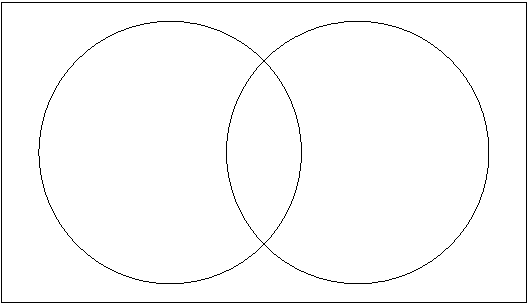
\includegraphics{./general_Venn.pdf}%
\end{picture}%
\setlength{\unitlength}{3947sp}%
%
\begingroup\makeatletter\ifx\SetFigFont\undefined%
\gdef\SetFigFont#1#2#3#4#5{%
  \reset@font\fontsize{#1}{#2pt}%
  \fontfamily{#3}\fontseries{#4}\fontshape{#5}%
  \selectfont}%
\fi\endgroup%
\begin{picture}(4224,2424)(2389,-2773)
\put(2926,-736){\makebox(0,0)[lb]{\smash{{\SetFigFont{12}{14.4}{\familydefault}{\mddefault}{\updefault}{\color[rgb]{0,0,0}A}%
}}}}
\put(6001,-736){\makebox(0,0)[lb]{\smash{{\SetFigFont{12}{14.4}{\familydefault}{\mddefault}{\updefault}{\color[rgb]{0,0,0}B}%
}}}}
\end{picture}%

\end{exer}

There is a connection, perhaps obvious, between the regions we
see in a Venn diagram with sets in general position and the recognizers
we studied in the section on digital logic circuits.  In fact both
of these topics have to do with \index{disjunctive normal form}\emph{disjunctive normal form}.  In a Venn diagram with $k$ sets, we are seeing the universe
of discourse broken up into the union of $2^k$ regions each of which 
corresponds to an intersection of either one of the sets or its complement.
An arbitrary expression involving set-theoretic symbols and these $k$ sets
is true in certain of these $2^k$ regions and false in the others.  
We have put the arbitrary expression in disjunctive normal form when
we express it as a union of the intersections that describe those regions.

\vspace{.1in}

\begin{picture}(0,0)%
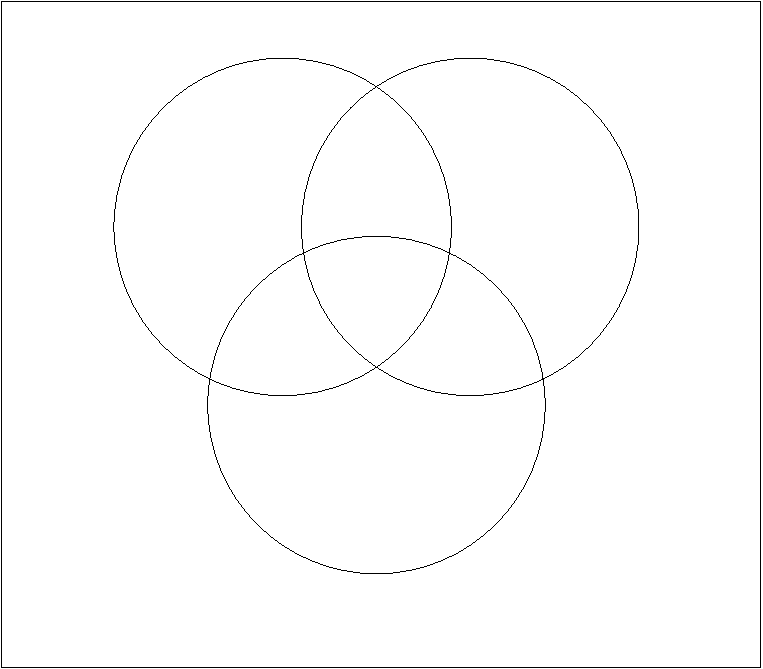
\includegraphics{figures/3set_Venn_gen_pos.pdf}%
\end{picture}%
\setlength{\unitlength}{3947sp}%
%
\begingroup\makeatletter\ifx\SetFigFont\undefined%
\gdef\SetFigFont#1#2#3#4#5{%
  \reset@font\fontsize{#1}{#2pt}%
  \fontfamily{#3}\fontseries{#4}\fontshape{#5}%
  \selectfont}%
\fi\endgroup%
\begin{picture}(6099,5349)(1189,-5398)
\put(1276,-286){\makebox(0,0)[lb]{\smash{{\SetFigFont{12}{14.4}{\familydefault}{\mddefault}{\updefault}{\color[rgb]{0,0,0}$U$}%
}}}}
\put(2326,-1486){\makebox(0,0)[lb]{\smash{{\SetFigFont{12}{14.4}{\familydefault}{\mddefault}{\updefault}{\color[rgb]{0,0,0}$A\cap\overline{B}\cap\overline{C}$}%
}}}}
\put(3751,-1711){\makebox(0,0)[lb]{\smash{{\SetFigFont{12}{14.4}{\familydefault}{\mddefault}{\updefault}{\color[rgb]{0,0,0}$A\cap B\cap\overline{C}$}%
}}}}
\put(3751,-2311){\makebox(0,0)[lb]{\smash{{\SetFigFont{12}{14.4}{\familydefault}{\mddefault}{\updefault}{\color[rgb]{0,0,0}$A\cap B\cap C$}%
}}}}
\put(3001,-2986){\makebox(0,0)[lb]{\smash{{\SetFigFont{12}{14.4}{\familydefault}{\mddefault}{\updefault}{\color[rgb]{0,0,0}$A\cap\overline{B}\cap C$}%
}}}}
\put(1351,-4561){\makebox(0,0)[lb]{\smash{{\SetFigFont{12}{14.4}{\familydefault}{\mddefault}{\updefault}{\color[rgb]{0,0,0}$\overline{A}\cap\overline{B}\cap\overline{C}$}%
}}}}
\put(2326,-811){\makebox(0,0)[lb]{\smash{{\SetFigFont{12}{14.4}{\familydefault}{\mddefault}{\updefault}{\color[rgb]{0,0,0}$A$}%
}}}}
\put(6001,-811){\makebox(0,0)[lb]{\smash{{\SetFigFont{12}{14.4}{\familydefault}{\mddefault}{\updefault}{\color[rgb]{0,0,0}$B$}%
}}}}
\put(4426,-4861){\makebox(0,0)[lb]{\smash{{\SetFigFont{12}{14.4}{\familydefault}{\mddefault}{\updefault}{\color[rgb]{0,0,0}$C$}%
}}}}
\put(4501,-2986){\makebox(0,0)[lb]{\smash{{\SetFigFont{12}{14.4}{\familydefault}{\mddefault}{\updefault}{\color[rgb]{0,0,0}$\overline{A}\cap B\cap C$}%
}}}}
\put(3751,-3736){\makebox(0,0)[lb]{\smash{{\SetFigFont{12}{14.4}{\familydefault}{\mddefault}{\updefault}{\color[rgb]{0,0,0}$\overline{A}\cap\overline{B}\cap C$}%
}}}}
\put(4951,-1486){\makebox(0,0)[lb]{\smash{{\SetFigFont{12}{14.4}{\familydefault}{\mddefault}{\updefault}{\color[rgb]{0,0,0}$\overline{A}\cap B\cap\overline{C}$}%
}}}}
\end{picture}%

 

\clearpage 

\noindent{\large \bf Exercises --- \thesection\ }

\begin{enumerate}
\item  Venn diagrams are usually made using simple closed curves 
with no further restrictions.  Try creating Venn diagrams for 3, 4 and
5 sets (in general position) using rectangular simple closed curves.

\hint{I found it easier to experiment by making my drawings on graph paper.  I never did  
manage to draw the $5$ set Venn diagram with just rectangles\ldots probably just a lack of persistence.}

\item  We call a curve \emph{rectilinear} if it is made
of line segments that meet at right angles.  Use rectilinear
simple closed curves to create a Venn diagram for 5 sets.

\hint{Of course, rectangles are rectilinear, so one could use the solution from the previous
problem (if, unlike me, you were persistant enough to find it).  Otherwise, 
start with the $4$ set diagram made with rectangles and use your $5$th (rectilinear) curve to split
each region into $2$ -- don't forget to split the region on the outside too.}

\item  Argue as to why rectilinear curves will suffice to build
any Venn diagram.

\hint{Fortunately the instructions don't say to {\em prove} that rectilinear curves will always
suffice, so we can be less rigorous.  Try to argue as to why it will alway be possible to add one more rectilinear curve to an existing Venn diagram and split every region into two.}

\item  Find the disjunctive normal form of $A \cap (B \cup C)$.

\hint{ $ (A \cap B \cap \overline{C}) \cup (A \cap \overline{B} \cap C) $ }

\item  Find the disjunctive normal form of $(A \triangle B) \triangle C$

\hint{It is $(A \cap \overline{B} \cap \overline{C}) \cup (\overline{A} \cap B \cap \overline{C}) \cup (\overline{A} \cap \overline{B} \cap C)$.  Now find the disjunctive normal form of 
$A \triangle (B \triangle C)$.}

\item The prototypes for the \emph{modus ponens} and \emph{modus tollens}
argument forms are the following:

\begin{tabular}{lcl}
\begin{minipage}{.3\textwidth}All men are mortal. \newline %
Socrates is a man. \newline
Therefore Socrates is mortal.\end{minipage} & \rule{16pt}{0pt} and \rule{16pt}{0pt} & %
 \begin{minipage}{.3\textwidth}All men are mortal. \newline %
Zeus is not mortal. \newline
Therefore Zeus is not a man.\end{minipage}
\end{tabular}

Illustrate these arguments using Venn diagrams.

\hint{The statement ``All men are mortal'' would be interpreted on a Venn diagram by showing the
set of ``All men'' as being entirely contained within the set of ``mortal beings.''   Socrates is an 
element of the inner set.  Zeus, on the other hand, lies outside of the outer set.}
 
\item Use Venn diagrams to convince yourself of the validity of
the following containment statement

\[ (A \cap B) \cup (C \cap D) \; \subseteq \; (A \cup C) \cap (B \cup D).\]

Now prove it!
 
\hint{Obviously we'll need one of the $4$-set Venn diagrams.}
 
\item Use Venn diagrams to show that the following set equivalence is false.

\[ (A \cup B) \cap (C \cup D) \; = \; (A \cup C) \cap (B \cup D) \]

\hint{After constructing Venn diagrams for both sets you should be able to see that there
are $4$ regions where they differ.  One is $A \cap B \cap \overline{C} \cap \overline{D}$.
What are the other three?}

\end{enumerate}



%% Emacs customization
%% 
%% Local Variables: ***
%% TeX-master: "GIAM-hw.tex" ***
%% comment-column:0 ***
%% comment-start: "%% "  ***
%% comment-end:"***" ***
%% End: ***



\newpage

\section{Russell's Paradox}
\label{sec:russell}

There is no Nobel prize category for mathematics.\footnote{There are prizes
considered equivalent to the Nobel in stature -- the Fields Medal, awarded every four years by the International Mathematical Union to up to four mathematical researchers under the age of forty, and the Abel Prize, awarded annually by the King of Norway.}   Alfred Nobel's will
called for the awarding of annual prizes in physics, chemistry, physiology 
or medicine, literature, and peace.  Later, the 
``Bank of Sweden Prize in Economic Sciences in Memory of Alfred Nobel'' 
was created and certainly several mathematicians have won what is 
improperly known as the Nobel prize in Economics.  But, there is no 
Nobel prize in Mathematics per se.  There is an interesting urban myth that
purports to explain this lapse: Alfred Nobel's wife either left him for, or
had an affair with a mathematician --- so Nobel, the inventor of dynamite
and an immensely wealthy and powerful man, when he decided to endow 
a set of annual prizes for ``those who, during the preceding year, shall have conferred the greatest benefit on mankind'' pointedly left out mathematicians.

One major flaw in this theory is that Nobel was never married.

In all likelihood, Nobel simply didn't view mathematics as a field
which provides benefits for mankind --- at least not directly. 
The broadest division within mathematics is between the ``pure''
and ``applied'' branches.  Just precisely where the dividing line
between these spheres lies is a matter of opinion, but it can be
argued that it is so far to one side that one may as well call an
applied mathematician a physicist 
(or chemist, or biologist, or economist, or \ldots).  One thing is
clear, Nobel believed to a certain extent in the utilitarian ethos.
The value of a thing (or a person) is determined by how useful it is (or they 
are), which makes it interesting that one of the few mathematicians
to win a Nobel prize was Bertrand Russell (the 1950 prize in Literature
 ``in recognition of his varied and significant writings in which he 
champions humanitarian ideals and freedom of thought''). 
 
Bertrand Russell was one of the twentieth century's most colorful
intellectuals.  He helped revolutionize the foundations of mathematics,
but was perhaps better known as a philosopher.  It's hard to conceive 
of \emph{anyone} who would characterize Russell as an applied mathematician!

Russell was an ardent anti-war and anti-nuclear activist.  He achieved a
status (shared with Albert Einstein, but very few others) as an eminent
scientist who was also a powerful moral authority.  Russell's mathematical
work was of a very abstruse foundational sort; he was concerned with
the idea of reducing all mathematical thought to Logic and Set theory.

In the beginning of our investigations into Set theory we mentioned 
that the notion of a ``set of all sets'' leads to something paradoxical.
Now we're ready to look more closely into that remark and hopefully 
gain an understanding of Russell's paradox.

By this point you should be okay with the notion of a set that 
contains other sets, but would it be okay for a set to contain
\emph{itself}?  That is, would it make sense to have a set 
defined by

\[ A = \{ 1, 2, A \}? \]

\noindent The set $A$ has three elements, $1$, $2$ and itself.  So we
could write

\[ A = \{ 1, 2, \{ 1, 2, A \} \}, \]
 
\noindent and then

\[ A = \{ 1, 2, \{ 1, 2, \{ 1, 2, A \} \} \}, \]

\noindent and then

\[ A = \{ 1, 2, \{ 1, 2, \{ 1, 2, \{ 1, 2, A \} \} \} \}, \]
  
\noindent et cetera.

This obviously seems like a problem.  Indeed, often paradoxes seem to
be caused by self-reference of this sort.  Consider 

\begin{center} 
\framebox[1.1\width]{The sentence in this box is false.}  
\end{center}

So a reasonable alternative
is to ``do'' math among the sets that don't exhibit this particular
pathology.  

Thus, inside the set of all sets we are singling out a particular subset
that consists of sets which don't contain themselves.  

\[ {\mathcal S} = \{ A \suchthat \; A \,\mbox{is a set} \; \land \; A \notin A \} \]

Now within the universal set we're working in (the set of all sets) there
are only two possibilities: a given set is either in ${\mathcal S}$ or
it is in its complement $\overline{\mathcal S}$.  Russell's paradox 
comes about when we try to decide which of these alternatives pertains
to ${\mathcal S}$ itself, the problem is that each alternative leads us 
to the other!

If we assume that ${\mathcal S} \in {\mathcal S}$, then it must be the 
case that ${\mathcal S}$ satisfies the membership criterion for ${\mathcal S}$.
Thus, ${\mathcal S} \notin {\mathcal S}$.

On the other hand, if we assume that ${\mathcal S} \notin {\mathcal S}$,
then we see that ${\mathcal S}$ does indeed satisfy the membership criterion for ${\mathcal S}$.  Thus ${\mathcal S} \in {\mathcal S}$.

Russell himself developed a workaround for the paradox which
bears his name.  Together with Alfred North Whitehead he published
a 3 volume work entitled \emph{Principia Mathematica}\footnote{Isaac Newton
also published a 3 volume work which is often cited by this same title,
\emph{Philosophiae Naturalis Principia Mathematica}.} \cite{PM}.  
In the Principia, Whitehead and Russell develop a system known as 
\emph{type theory} which sets forth principles for avoiding problems
like Russell's paradox.  Basically, a set and its elements are of
different ``types'' and so the notion of a set being contained in itself
(as an element) is disallowed.

\clearpage 

\noindent{\large \bf Exercises --- \thesection\ }

\begin{enumerate}
\item Verify that $(A \implies {\lnot}A) \land ({\lnot}A \implies A)$
is a logical contradiction in two ways:  by filling out a truth table and 
using the laws of logical equivalence.

\hint{In order to get started on this you'll need to convert the conditionals into equivalent
disjunctions.  Recall that $X \implies Y \; \equiv \; {\lnot}X \lor Y$.}

\item One way out of Russell's paradox is to declare that the collection
of sets that don't contain themselves as elements is not a set itself.
Explain how this circumvents the paradox. 

\hint{If it's not a set then it doesn't necessarily have to have the property that we
can be {\em sure} whether an element is in it or not.}

\end{enumerate}


%% Emacs customization
%% 
%% Local Variables: ***
%% TeX-master: "GIAM-hw.tex" ***
%% comment-column:0 ***
%% comment-start: "%% "  ***
%% comment-end:"***" ***
%% End: ***



%\newpage
%
%\renewcommand{\bibname}{References for chapter 4}
%\bibliographystyle{plain}
%\bibliography{main}

%% Emacs customization
%% 
%% Local Variables: ***
%% TeX-master: "GIAM.tex" ***
%% comment-column:0 ***
%% comment-start: "%% "  ***
%% comment-end:"***" ***
%% End: ***



\chapter{Proof techniques II --- Induction}
\label{ch:proof2}

{\em Who was the guy who first looked at a cow and said, "I think I'll drink whatever comes out of these things when I squeeze 'em!"? --Bill Watterson}

\section{The principle of mathematical induction}
\label{sec:induct}

The \index{induction}Principle of Mathematical Induction (PMI) may be the least intuitive
proof method available to us.  Indeed, at first, PMI may feel somewhat like
grabbing yourself by the seat of your pants and lifting yourself into
the air.  Despite the indisputable fact that proofs by PMI often feel
like magic, we need to convince you of the validity of this proof
technique.  It is one of the most important tools in your mathematical
kit!

The simplest argument in favor of the validity of PMI is simply that it is
axiomatic.  This may seem somewhat unsatisfying, but the axioms for
the natural number system, known as the \index{Peano axioms}Peano axioms,
include one that justifies PMI.  The Peano axioms will not be treated 
thoroughly in this book, but here they are:

\begin{enumerate}
\item[i)] There is a least element of $\Naturals$ that we denote by $0$.
\item[ii)] Every natural number $a$ has a successor denoted by $s(a)$.
(Intuitively, think of $s(a) = a+1$.)
\item[iii)] There is no natural number whose successor is $0$.  (In other
words, -1 isn't in $\Naturals$.)
\item[iv)] Distinct natural numbers have distinct successors.  
($a \neq b \; \implies \; s(a) \neq s(b)$) 
\item[v)] If a subset of the natural numbers contains $0$ and also has the
property that whenever $a \in S$ it follows that $s(a) \in S$, then the
subset $S$ is actually equal to $\Naturals$.   
\end{enumerate}

The last axiom is the one that justifies PMI.  Basically, if $0$ is in
a subset, and the subset has this property about successors\footnote{Whenever a number is in it, the number's successor must be in it.}, then $1$ must
be in it.  But if $1$ is in it, then $1$'s successor ($2$) must be in it.
And so on \ldots  

The subset ends up having every natural number in it.

\begin{exer}
Verify that the following symbolic formulation has the same content
as the version of the 5th Peano axiom given above.
\[ \forall S \subseteq \Naturals \; ( 0 \in S ) \land (\forall a \in \Naturals, a \in S \, \implies s(a) \in S) \implies  \; S=\Naturals \]

\end{exer}
\bigskip

On August 16th 2003, \index{Lihua, Ma}Ma Lihua of Beijing, China earned her place in the 
record books by single-handedly setting up an arrangement of dominoes 
standing on end (actually, the setup took 7 weeks and was almost ruined by
some cockroaches in the Singapore Expo Hall) and toppling them.  
After the first domino was tipped over it took about six minutes
before 303,621 out of the 303,628 dominoes had fallen. (One has to wonder 
what kept those other 7 dominoes upright \ldots)  

\begin{center}
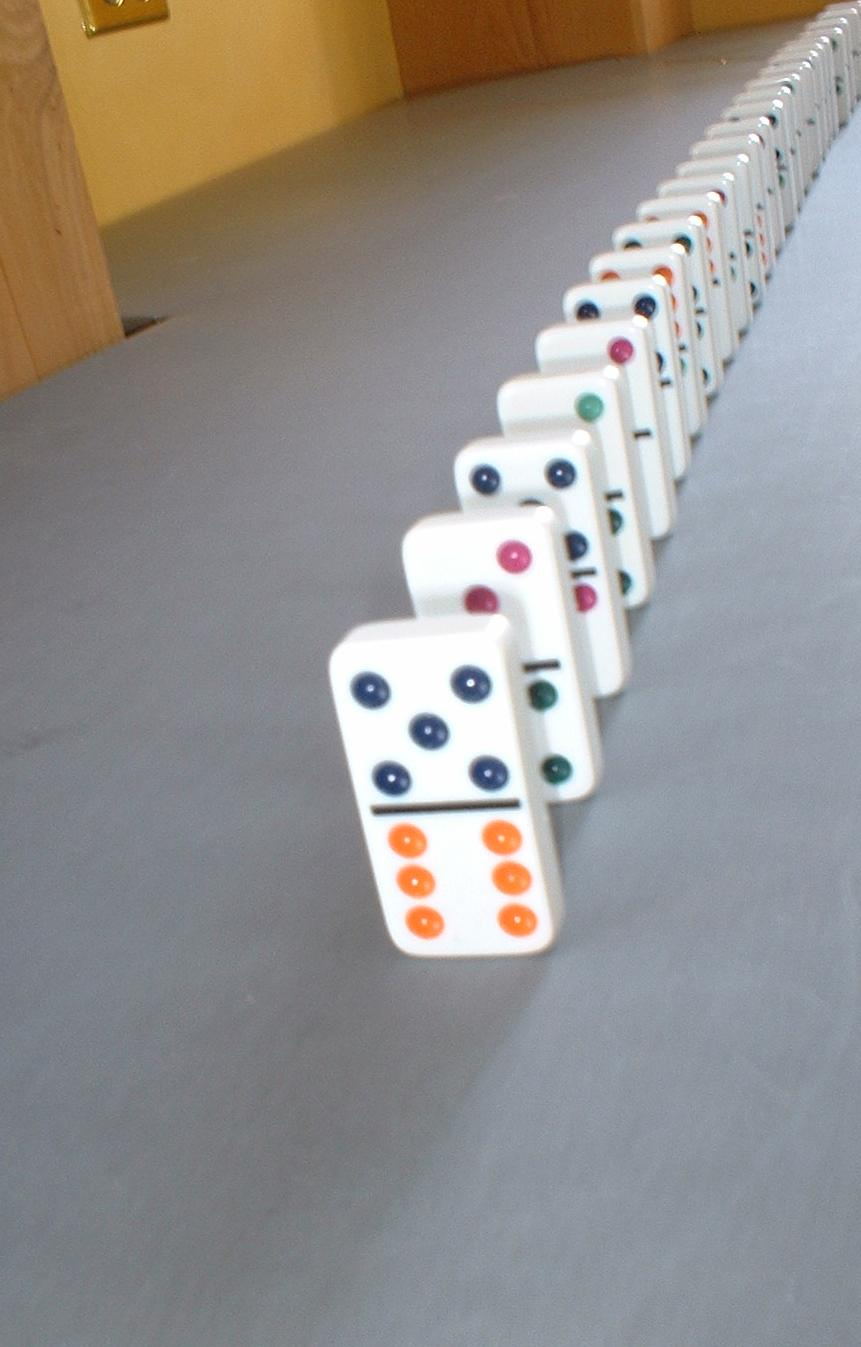
\includegraphics[scale=.2]{photos/domino_row.jpg}
\end{center}

This is the model one should keep in mind when thinking about PMI: domino
toppling.  In setting up a line of dominoes, what do we need to do
in order to ensure that they will all fall when the toppling begins?
Every domino must be placed so that it will hit and topple its successor.
This is exactly analogous to $(a \in S \, \implies s(a) \in S)$.  (Think 
of $S$ having the membership criterion, $x \in S$ = ``$x$ will have fallen
when the toppling is over.'')   The other thing that has to happen
(barring the action of cockroaches) is for someone to knock over the
first domino.  This is analogous to $0 \in S$.

Rather than continuing to talk about subsets of the naturals, it will
be convenient to recast our discussion in terms of infinite families
of logical statements.  If we have a sequence of statements, (one
for each natural number) $P_0$, $P_1$, $P_2$, $P_3$, \ldots  we
can prove them \emph{all} to be true using PMI.  We have to do two
things.   First -- and this is usually the easy part -- we must show 
that $P_0$ is true (i.e. the first domino \emph{will} get knocked over).
Second, we must show, for every possible value of $k$, $P_k \implies P_{k+1}$
(i.e. each domino will knock down its successor).  These two parts 
of an inductive proof are known, respectively, as the \emph{basis}
and the \emph{inductive step}. 

An outline for a proof using PMI:

\begin{center}
\begin{tabular}{|c|} \hline
\rule{16pt}{0pt}\begin{minipage}{.75\textwidth}

\rule{0pt}{16pt}{\bf \large Theorem} $ \displaystyle \forall n \in \Naturals, \; P_n $
\medskip

\rule{0pt}{20pt} {\em Proof:} (By induction)

\noindent {\bf Basis:}

\begin{center}
$\vdots$ \rule{36pt}{0pt} \begin{minipage}[c]{1.7 in} (Here we must show that $P_0$ is true.) \end{minipage}
\end{center}

\noindent {\bf Inductive step:}

\begin{center}
$\vdots$ \rule{36pt}{0pt} \begin{minipage}[c]{1.7 in} (Here we must show that $\forall k,  P_k \implies P_{k+1}$ is true.) \end{minipage}
\end{center}

\rule{0pt}{0pt} \hspace{\fill} Q.E.D. \rule[-10pt]{0pt}{16pt}
\end{minipage} \rule{16pt}{0pt} \\ \hline
\end{tabular}
\end{center}
\medskip

Soon we'll do an actual example of an inductive 
proof, but first we have to say something \emph{REALLY IMPORTANT}
about such proofs.  Pay attention! This is \emph{REALLY IMPORTANT}!
When doing the second part of an inductive proof (the inductive step),
you are proving a UCS, and if you recall how that's done, you start
by assuming the antecedent is true.  But the particular UCS we'll
be dealing with is $\forall k,  P_k \implies P_{k+1}$.  That means
that in the course of proving $\forall n,  P_n$ we have to \emph{assume}
 that $P_k$ is true.  Now this sounds very much like the error known
as ``circular reasoning,'' especially as many authors don't even
use different letters ($n$ versus $k$ in our outline) to distinguish
the two statements.  (And, quite honestly, we only introduced the variable
$k$ to assuage a certain lingering guilt regarding circular reasoning.)
The sentence $\forall n,  P_n$ is what we're trying to prove, but the
sentence we need to prove in order to do that is $\forall k,  P_k \implies P_{k+1}$.
This is subtly different -- in proving that $\forall k,  P_k \implies P_{k+1}$
(which is a UCS!) we assume that $P_k$ is true {\em for some particular value of $k$}.

The sentence $P_k$ is known as the 
\index{inductive hypothesis}\emph{inductive hypothesis}.
Think about it this way:  If we were doing an entirely separate
proof of $\forall n,  P_n \implies P_{n+1}$, it would certainly be fair
to use the inductive hypothesis, and \emph{once that proof was done}, 
it would be okay to quote that result in an inductive proof of 
$\forall n,  P_n$.  Thus we can compartmentalize our way out of the
difficulty!

Okay, so on to an example.  In Section~\ref{sec:basic_set_notions} 
we discovered a formula relating the sizes of a set $A$ and its 
power set ${\mathcal P}(A)$.  If $|A| = n$ then $|{\mathcal P}(A)| = 2^n$.
What we've got here is an infinite family of logical sentences, one for 
each value of $n$ in the natural numbers,

\[ |A| = 0 \implies |{\mathcal P}(A)| = 2^0, \]
\[ |A| = 1 \implies |{\mathcal P}(A)| = 2^1, \]
\[ |A| = 2 \implies |{\mathcal P}(A)| = 2^2, \]
\[ |A| = 3 \implies |{\mathcal P}(A)| = 2^3, \]

\noindent et cetera.

This is exactly the sort of situation in which we use induction.

\begin{thm} For all finite sets $A$, $\displaystyle |A| = n \implies  |{\mathcal P}(A)| = 2^n$.
\end{thm}

\begin{proof}
Let $n = |A|$ and proceed by induction on $n$.

\noindent {\bf Basis:} Suppose $A$ is a finite set and $|A| = 0$, it follows 
that $A = \emptyset$.  The power set of $\emptyset$ is $\{ \emptyset \}$ 
which is a set having 1 element.  Note that $2^0 = 1$.
   
\noindent {\bf Inductive step:}  Suppose that $A$ is a finite set with $|A| = k+1$.  Choose some particular element of $A$, say $a$, and note that
we can divide the subsets of $A$ (i.e. elements of ${\mathcal P}(A)$) into
two categories, those that contain $a$ and those that don't.

Let $S_1 = \{ X \in {\mathcal P}(A) \suchthat a \in X \}$ and let
$S_2 = \{ X \in {\mathcal P}(A) \suchthat a \notin X \}$.  We have 
created two sets that contain all the elements of ${\mathcal P}(A)$,
and which are disjoint from one another.  In symbolic form, 
$S_1 \cup S_2 = {\mathcal P}(A)$ and $S_1 \cap S_2 = \emptyset$.
It follows that $|{\mathcal P}(A)| = |S_1| + |S_2|$.  

Notice that $S_2$ is actually the power set of the $k$-element set
$A \setminus \{ a \}$.  By the inductive hypothesis, $|S_2| = 2^k$.
Also, notice that each set in $S_1$ corresponds uniquely to a set in
$S_2$ if we just remove the element $a$ from it.  This shows that 
$|S_1| = |S_2|$.  Putting this all together we get that 
$|{\mathcal P}(A)| = 2^k + 2^k = 2(2^k) = 2^{k+1}$.

\end{proof}

Here are a few pieces
of advice about proofs by induction:

\begin{itemize}
\item Statements that can be proved inductively don't always start out with 
$P_0$.  Sometimes $P_1$ is the first statement in an infinite family.
Sometimes its $P_5$.  Don't get hung up about something that could be
handled by renumbering things.  
\item In your final write-up you only need to prove the initial case
(whatever it may be) for the basis, but it is a good idea to try 
the first several cases while you are in the ``draft'' stage.  This
can provide insights into how to prove the inductive step, and it may
also help you avoid a classic error in which the inductive approach fails
essentially just because there is a gap between two of the earlier 
dominoes.\footnote{See exercise~\ref{ex:horses}, the classic fallacious proof that all horses are the same color.}
\item It is a good idea to write down somewhere just what it is that
needs to be proved in the inductive step --- just don't make it look like 
you're assuming what needs to be shown.  For instance in the proof above
it might have been nice to start the inductive step with a comment along
the following lines, ``What we need to show is that under the assumption
that any set of size $k$ has a power set of size $2^k$, it follows that
a set of size $k+1$ will have a power set of size $2^{k+1}$.'' 
\end{itemize}
\medskip

We'll close this section with a short discussion about nothing.

\ifthenelse{\boolean{ZeroInNaturals}}{
When we first introduced the natural numbers ($\Naturals$) in Chapter~\ref{ch:intro} we decided to follow the convention that the smallest natural number is 1.
You may have noticed that the Peano axioms mentioned in the beginning of this
section treat $0$ as the smallest natural number.  So, from here on out we
are going to switch things up and side with Dr. Peano.  That is, from now
on we will use the convention

\[\Naturals \, = \, \{ 0, 1, 2, 3, \ldots \} \]

Hmmm\ldots \rule{5pt}{0pt}Maybe that was a short discussion about {\em something} after all.
}{
When we first introduced the natural numbers ($\Naturals$) in Chapter~\ref{ch:intro} we decided to follow the convention that the smallest natural number is 1.
You may have noticed that the Peano axioms mentioned in the beginning of this
section treat $0$ as the smallest natural number.  Many people follow Dr.\ Peano's
convention, but we're going to stick with our original interpretation:

\[\Naturals \, = \, \{ 1, 2, 3, \ldots \} \]

\renewcommand{\Naturals}{{\mathbb Z}^{\mbox{\tiny noneg}} }

Despite our stubbornness, we are forced to admit that many inductive proofs are
made easier by treating the ``first'' case as being in truth the one numbered $0$.   We'll
use the symbol $\Naturals$ to indicate the set ${\mathbb N} \cup \{ 0 \}$.
}

\newpage

  
\noindent{\large \bf Exercises --- \thesection\ }

\begin{enumerate}
\item Consider the sequence of number that are 1 greater than a multiple of 4.
(Such numbers are of the form $4j+1$.)

\[ 1, 5, 9, 13, 17, 21, 25, 29, \ldots \]

The sum of the first several numbers in this sequence can be expressed as
a polynomial.

\[ \sum_{j=0}^n 4j+1 = 2n^2 + 3n + 1 \]

Complete the following table in order to provide evidence that the formula
above is correct.

\begin{center}
\begin{tabular}{c|c|c}
$n$ & $\sum_{j=0}^n 4j+1$ & $2n^2 + 3n + 1$ \\ \hline
 0 & $1$ & $1$ \\
 1 & $1 + 5 = 6$ &  $2 \cdot 1^2 + 3 \cdot 1 + 1 = 6$ \\
 2 & $1 + 5 + 9 = \rule{15pt}{0pt}$ \hint{$15$} &  \hint{$2 \cdot 2^2 + 3 \cdot 2 + 1 = 15$}\\
 3 & \hint{$1 + 5 + 9 + 13 = 28$} &  \hint{$2 \cdot 3^2 + 3 \cdot 3 + 1 = 28$}\\
 4 & & \\
\end{tabular}
\end{center}

\hint{I'm leaving the very last one for you to do.}


\item \label{ex:horses} What is wrong with the following inductive proof of
``all horses are the same color.''?

{\bf Theorem} Let $H$ be a set of $n$ horses, all horses in $H$ 
are the same color.

\begin{proof}
We proceed by induction on $n$.

\noindent {\bf Basis: } Suppose $H$ is a set containing 1 horse.  Clearly
this horse is the same color as itself.

\noindent {\bf Inductive step: } Given a set of $k+1$ horses $H$ we can 
construct two sets of $k$ horses.  Suppose $H = \{ h_1, h_2, h_3, \ldots h_{k+1} \}$.  Define $H_a = \{ h_1, h_2, h_3, \ldots h_{k} \}$ (i.e. $H_a$ contains
just the first $k$ horses) and $H_b = \{ h_2, h_3, h_4, \ldots h_{k+1} \}$ 
(i.e. $H_b$ contains the last $k$ horses).  By the inductive hypothesis
both these sets contain horses that are ``all the same color.''  Also,
all the horses from $h_2$ to $h_k$ are in both sets so both $H_a$ and
$H_b$ contain only horses of this (same) color.  Finally, we conclude that
all the horses in $H$ are the same color.

\end{proof}
\medskip
   
\hint{Look carefully at the stage from $n=2$ to $n=3$.}

\hintspagebreak

\item For each of the following theorems, write the statement that must be
proved for the basis -- then prove it, if you can!

\begin{enumerate}
\item The sum of the first $n$ positive integers is $(n^2+n)/2$.

\hint{The sum of the first $0$ positive integers is $(0^2 + 0)/2$.  Or, if you
prefer to start with something rather than nothing: The sum of the first $1$ positive integers
is $(1^2+1)/2$. }

\item The sum of the first $n$ (positive) odd numbers is $n^2$.

\hint{The sum of the first $0$ positive odd numbers is $0^2$.  Or, the sum of the first $1$ positive odd numbers is $1^2$.}

\item If $n$ coins are flipped, the probability that all of them 
are ``heads'' is $1/2^n$.

\hint{If $1$ coin is flipped, the the probability that it is ``heads'' is $1/2$. Or if we try it 
when $n=0$, ``If no coins are flipped the probability that all t=of them are heads is 1.  Does that
make sense to you?  Is it reasonable that we would say it is 100\% certain that all of the coins
are heads in a set that doesn't contain {\em any} coins? }

\item Every $2^n \times 2^n$ chessboard -- with one square removed -- can 
be tiled perfectly\footnote{Here, ``perfectly tiled'' means that every trominoe
covers 3 squares of the chessboard (nothing hangs over the edge) and that every
square of the chessboard is covered by some trominoe.} by L-shaped trominoes.  
(A trominoe is like a domino but 
made up of $3$ little squares.  There are two kinds, straight 
\begin{picture}(0,0)%
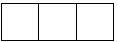
\includegraphics{figures/straight_trominoe.pdf}%
\end{picture}%
\setlength{\unitlength}{3947sp}%
%
\begingroup\makeatletter\ifx\SetFigFont\undefined%
\gdef\SetFigFont#1#2#3#4#5{%
  \reset@font\fontsize{#1}{#2pt}%
  \fontfamily{#3}\fontseries{#4}\fontshape{#5}%
  \selectfont}%
\fi\endgroup%
\begin{picture}(924,324)(1189,-673)
\end{picture}%
 and L-shaped 
\begin{picture}(0,0)%
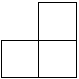
\includegraphics{figures/L-shaped_trominoe.pdf}%
\end{picture}%
\setlength{\unitlength}{3947sp}%
%
\begingroup\makeatletter\ifx\SetFigFont\undefined%
\gdef\SetFigFont#1#2#3#4#5{%
  \reset@font\fontsize{#1}{#2pt}%
  \fontfamily{#3}\fontseries{#4}\fontshape{#5}%
  \selectfont}%
\fi\endgroup%
\begin{picture}(624,624)(1189,-673)
\end{picture}%
. This problem is only concerned with
the L-shaped trominoes.)
\end{enumerate}

\hint{If $n=1$ we have: ``Every $2 \times 2$ chessboard -- with one square removed
can be tiled perfectly by L-shaped trominoes.  This version is trivial to prove.  Try formulating
the $n=0$ case.}
  
\hintspagebreak

\item Suppose that the rules of the game for PMI were changed so that one
did the following:
\begin{itemize}
\item Basis.  Prove that $P(0)$ is true.
\item Inductive step.  Prove that for all $k$, $P_k$ implies $P_{k+2}$
\end{itemize}


\noindent Explain why this would not constitute a valid proof that $P_n$ holds 
for all natural numbers $n$. 
\noindent How could we change the basis in this outline to obtain a valid proof?

\hint{In this modified version, $P(0)$ is not going to imply $P(1)$. and in fact, none of the odd numbered
statements will be proven.  If we change the 
basis so that we prove both $P(0$ and $P(1)$, all the even statements will be implied by
$P(0$ being true and all the odd statements get forced because $P(1)$ is true.}

\item If we wanted to prove statements that were indexed by the integers,

\[ \forall z \in \Integers, \; P_z, \]

\noindent what changes should be made to PMI?

\hint{A quick change would be to replace $\forall k, \; P_k \implies P_{k+1}$ in the inductive
step with $\forall k, \; P_k \iff P_{k+1}$.  While this would do the trick, a slight improvement 
is possible, if we treat the positive and negative cases for $k$ seperately.}
 
\end{enumerate}


%% Emacs customization
%% 
%% Local Variables: ***
%% TeX-master: "GIAM-hw.tex" ***
%% comment-column:0 ***
%% comment-start: "%% "  ***
%% comment-end:"***" ***
%% End: ***



 
\newpage

\section{Formulas for sums and products}

Gauss, when only a child, found a formula for
summing the first 100 natural numbers (or so the story goes\ldots). 
This formula, and his clever method for justifying it, can be easily 
generalized to the sum of the first $n$ naturals.
While learning calculus, notably during the study of Riemann sums,
one encounters other summation formulas.  For example, in approximating the
integral of the function $f(x)=x^2$ from $0$ to $100$ one needs the sum of 
the first 100 {\em squares}.  For this reason, somewhere in almost
every calculus book one will find the following formulas collected:

\begin{gather*}
\sum_{j=1}^n j = \frac{n(n+1)}{2}\\
\sum_{j=1}^n j^2 = \frac{n(n+1)(2n+1)}{6}\\
\sum_{j=1}^n j^3 = \frac{n^2(n+1)^2}{4}.\\
\end{gather*}

\noindent A really industrious author might also include the sum of the 
fourth powers.  Jacob Bernoulli (a truly industrious individual)
got excited enough to find formulas for the sums of the first
ten powers of the naturals.  Actually, Bernoulli went much further.  His work
on sums of powers lead to the definition of what are now known as Bernoulli
numbers and let him calculate $\sum_{j=1}^{1000}j^{10}$ in 
about seven minutes --
long before the advent of calculators!  In \cite[p. 320]{struik}, Bernoulli is 
quoted:

\begin{quote}
With the help of this table it took me less than half of a quarter of an hour
to find that the tenth powers of the first 1000 numbers being added together 
will yield the sum 

\[ 91,409,924,241,424,243,424,241,924,242,500. \]

\end{quote}

To the beginning calculus student, the beauty of the above relationships may
be somewhat dimmed by the memorization challenge that they represent.  It
is fortunate then, that the right-hand side of the third formula is just 
the square of the right-hand side of the first formula.  And of course,
the right-hand side of the first formula is something that can be deduced 
by a six year old child (provided that he is a super-genius!)  This happy
coincidence leaves us to apply most of our rote memorization energy to
formula number two, because the first and third formulas are related by
the following rather bizarre-looking equation,

\[
\sum_{j=1}^n j^3 = \left( \sum_{j=1}^n j \right)^2. 
\]       

\noindent The sum of the cubes of the first $n$ numbers is the square of their sum.

For completeness we should include the following formula which 
should be thought of as the sum of the zeroth powers of the first $n$
naturals.

\[ \sum_{j=1}^n 1 = n \]

\begin{exer}
Use the above formulas to approximate the integral

\[ \int_{x=0}^{10} x^3 - 2x +3 \mbox{d}x \]
\end{exer}
\bigskip

Our challenge today is not to merely memorize these formulas but
to prove their validity.  We'll use PMI.

Before we start in on a proof, it's important to figure out where 
we're trying to go.  In proving the formula that Gauss discovered
by induction we need to show that the $k+1$--th version of the 
formula holds, assuming that the $k$--th version does.  Before
proceeding on to read the proof do the following

\begin{exer}
Write down the $k+1$--th version of the formula for the sum of
the first $n$ naturals.  (You have to replace every $n$ with 
a $k+1$.)
\end{exer}

\begin{thm}
\[ \forall n \in \Naturals, \; \sum_{j=1}^n j = \frac{n(n+1)}{2} \]
\end{thm}

\begin{proof}
We proceed by induction on $n$.

\noindent {\bf Basis: }  Notice that when $n=0$ the sum on the left-hand side
has no terms in it!  This is known as an \index{empty sum} empty sum, and by 
definition, an empty sum's value is $0$.   Also, when 
$n=0$ the formula on the right-hand side becomes $(0 \cdot 1)/2$ and this is 
$0$ as well.\footnote{If you'd prefer to avoid the ``empty sum'' argument, %
you can choose to use $n=1$ as the basis case.  The theorem should %
be restated so the universe of discourse is \emph{positive} naturals.}

\noindent {\bf Inductive step: }  Consider the sum on the left-hand side of
the $k+1$--th version of our formula.

\[ \sum_{j=1}^{k+1} j \]

We can separate out the last term of this sum.

\[ = (k+1) + \sum_{j=1}^{k} j \]

Next, we can use the inductive hypothesis to replace the sum (the part 
that goes from 1 to $k$) with a formula.

\[ = (k+1) + \frac{k(k+1)}{2} \]

From here on out it's just algebra \ldots

\[ = \frac{2(k+1)}{2} + \frac{k(k+1)}{2} \]

\[ = \frac{2(k+1) + k(k+1)}{2} \]

\[ = \frac{(k+1) \cdot (k+2)}{2}. \]

\end{proof}
\medskip

Notice how the inductive step in this proof works.  We start by writing
down the left-hand side of $P_{k+1}$, we pull out the last term
so we've got the left-hand side of $P_{k}$ (plus something else), then
we apply the inductive hypothesis and do some algebra until we arrive
at the right-hand side of $P_{k+1}$.  Overall, we've just transformed the
left-hand side of the statement we wish to prove into its right-hand side.

There is another way to organize the inductive steps in proofs like these
that works by manipulating entire equalities (rather than just one side
or the other of them).

\begin{quote}

\noindent {\bf Inductive step (alternate): }  By the inductive 
hypothesis, we can write

\[ \sum_{j=1}^{k} j = \frac{k(k+1)}{2}. \]

Adding $(k+1)$ to both side of this yields

\[ \sum_{j=1}^{k+1} j = (k+1) + \frac{k(k+1)}{2}. \]

Next, we can simplify the right-hand side of this to obtain

\[ \sum_{j=1}^{k+1} j = \frac{(k+1)(k+2)}{2}. \]

\rule{0pt}{0pt} \hspace{\fill} Q.E.D.
\end{quote}
\medskip

Oftentimes one can save considerable effort in an inductive 
proof by creatively using the factored form during intermediate steps.
On the other hand, sometimes it is easier to just simplify everything
completely, and also, completely simplify the expression on the 
right-hand side of $P(k+1)$ and then verify that the two things are
equal.  This is basically just another take on the technique of 
``working backwards from the conclusion.''  Just remember that 
in writing-up your proof you need to make it look as if you reasoned
directly from the premises to the conclusion.  We'll illustrate
what we've been discussing in this paragraph while proving
the formula for the sum of the squares of the first $n$ positive integers.

\begin{thm}
\[ \forall n \in \Zplus, \; \sum_{j=1}^n j^2 = \frac{n(n+1)(2n+1)}{6} \]
\end{thm}

\begin{proof}
We proceed by induction on $n$.

\noindent {\bf Basis: } When $n = 1$ the sum has only one term, $1^2 = 1$.
On the other hand, the formula is 
$\displaystyle \frac{1(1+1)(2\cdot 1+1)}{6} = 1$.  Since these are equal, the 
basis is proved.

\noindent {\bf Inductive step: }

\begin{tabular}{|ccc|} \hline
 & &\\
 & \begin{minipage}{4 in} 
Before proceeding with the inductive step, in this box, we will
figure out what the right-hand side of our theorem looks like 
when $n$ is replaced with $k+1$:
\begin{gather*}
 \frac{(k+1)((k+1)+1)(2(k+1)+1)}{6} \\
= \frac{(k+1)(k+2)(2k+3)}{6} \\
= \frac{(k^2+3k+2)(2k+3)}{6} \\
= \frac{2k^3+9k^2+13k+6}{6}.
\end{gather*}
\end{minipage} & \\ 
 & & \\ \hline
\end{tabular}


By the inductive hypothesis,

\[ \sum_{j=1}^k j^2 = \frac{k(k+1)(2k+1)}{6}. \]

Adding $(k+1)^2$ to both sides of this equation gives

\[ (k+1)^2 + \sum_{j=1}^k j^2 = \frac{k(k+1)(2k+1)}{6} + (k+1)^2. \]

Thus,

\[ \sum_{j=1}^{k+1} j^2 = \frac{k(k+1)(2k+1)}{6} + \frac{6(k+1)^2}{6}. \]

Therefore,

\begin{gather*}
\sum_{j=1}^{k+1} j^2 = \frac{(k^2+k)(2k+1)}{6} + \frac{6(k^2+2k+1)}{6} \\
 = \frac{(2k^3+3k^2+k)+(6k^2+12k+6)}{6}\\
 = \frac{2k^3+9k^2+13k+6}{6}\\
 = \frac{(k^2+3k+2)(2k+3)}{6}\\
 = \frac{(k+1)(k+2)(2k+3)}{6} \\
 = \frac{(k+1)((k+1)+1)(2(k+1)+1)}{6}.
\end{gather*}

This proves the inductive step, so the result is true.

\end{proof}

Notice how the last four lines of the proof are the same as those in
the box above containing our scratch work?  (Except in the reverse order.)

We'll end this section by demonstrating one more use of this technique.
This time we'll look at a formula for a product rather than a sum.

\begin{thm} $$\forall n \geq 2 \in \Integers, \prod_{j=2}^n \left( 1 - \frac{1}{j^2} \right) \;  = \; \frac{n+1}{2n}. $$
\end{thm}

Before preceding with the proof let's look at an example (although this 
has nothing to do with proving anything, it's really not a bad idea -- it can
keep you from wasting a lot of time trying to prove something that isn't 
actually true!)  When $n = 4$ the product is

\[  \left(1-\frac{1}{2^2}\right) \cdot \left(1-\frac{1}{3^2}\right) \cdot \left(1-\frac{1}{4^2}\right). 
\]

This simplifies to

\[ \left( 1-\frac{1}{4} \right) \cdot \left( 1-\frac{1}{9} \right) \cdot 
\left( 1-\frac{1}{16} \right) \quad = \quad \left( \frac{3}{4} \right) \cdot \left( \frac{8}{9} \right) \cdot \left( \frac{15}{16} \right) \quad = \quad \frac{360}{576}.
\]

The formula on the right-hand side is 

\[ \frac{4+1}{2 \cdot 4} \quad = \frac{5}{8}. \]

Well!  These two expressions are \emph{clearly} not equal to one another\ldots
What?  You say they are?  Just give me a second with my calculator\ldots

Alright then.  I guess we can't dodge doing the proof\ldots

\begin{proof}
(Using mathematical induction on $n$.)

\noindent {\bf Basis: } When $n = 2$ the product has only one term, $1-1/2^2 = 3/4$.
On the other hand, the formula is 
$\displaystyle \frac{2+1}{2\cdot2} = 3/4$.  Since these are equal, the 
basis is proved.

\noindent {\bf Inductive step: }

Let $k$ be a particular but arbitrarily chosen integer such that

\[ \prod_{j=2}^k \left( 1 - \frac{1}{j^2} \right) \;  = \; \frac{k+1}{2k}. \]

Multiplying\footnote{Really, the only reason I'm doing this silly proof is to 
point out to you that when you're doing the inductive step in a proof of a 
formula for a {\bf product}, you don't add to both sides anymore, you {\bf multiply.} You see that, right?  Well, consider yourself to have been pointed out to or \ldots oh, whatever.}  both sides by the $k+1$-th term of the product 
gives

\[ \left( 1 - \frac{1}{(k+1)^2} \right) \; \cdot \; \prod_{j=2}^k \left( 1 - \frac{1}{j^2} \right) \quad  = \quad \frac{k+1}{2k} \; \cdot \; \left( 1 - \frac{1}{(k+1)^2} \right). \]

Thus 

\[ \prod_{j=2}^{k+1} \left( 1 - \frac{1}{j^2} \right) \quad  = \quad \frac{k+1}{2k} \; \cdot \; \left( 1 - \frac{1}{(k+1)^2} \right) \]

\[ = \frac{k+1}{2k} - \frac{(k+1)}{2k(k+1)^2} \]

\[ = \frac{k+1}{2k} - \frac{(1)}{2k(k+1)} \]

\[ = \frac{(k+1)^2 - 1}{2k(k+1)} \]

\[ = \frac{k^2+2k}{2k(k+1)} \]

\[ = \frac{k (k+2)}{2k(k+1)} \]

\[ = \frac{k+2}{2(k+1)}. \]

\end{proof}

\newpage
  
\noindent{\large \bf Exercises --- \thesection\ }

\begin{enumerate}
\item Write an inductive proof of the formula for the sum 
of the first $n$ cubes.

\hint{
\begin{thm*}
\[ \forall n \in \Naturals, \; \sum_{k=1}^n k^3 \;= \; \left( \frac{n(n+1)}{2} \right)^2 \]
\end{thm*}

\begin{proof} (By mathematical induction)

{\bf Base case:} ($n=1$)
For the base case, note that when $n=1$ we have

\[ \sum_{k=1}^n k^3 \; = \; 1 \]

\noindent and 

\[ \left( \frac{n(n+1)}{2} \right)^2  \; = \; 1.\]

{\bf Inductive step:}

Suppose that $m>1$ is an integer such that 

\[ \sum_{k=1}^m k^3 \; = \; \left( \frac{m(m+1)}{2} \right)^2 \]

\noindent Add $(m+1)^3$ to both sides to obtain

\[ (m+1)^3 + \sum_{k=1}^m k^3 \;= \; \left( \frac{m(m+1)}{2} \right)^2 + (m+1)^3. \]

\noindent Thus

\begin{gather*} 
\sum_{k=1}^{m+1} k^3 \;= \; \left( \frac{m^2(m+1)^2}{4} \right) + \frac{4(m+1)^3}{4} \\
\;= \; \left( \frac{m^2(m+1)^2 + 4 (m+1)^3}{4} \right)\\
\; = \; \left( \frac{(m+1)^2 (m^2 + 4(m+1))}{4} \right)\\
\; = \; \left( \frac{(m+1)^2 (m^2 + 4m +4)}{4} \right)\\
\; = \; \left( \frac{(m+1)^2 (m+2)^2}{4} \right)\\
\; = \; \left( \frac{(m+1)(m+2)}{2} \right)^2
\end{gather*}

 \end{proof}
}

\wbvfill

\workbookpagebreak
  
\item Find a formula for the sum of the first $n$ fourth powers.

\hint{\[ \frac{n\cdot(n+1)\cdot(2n+1)\cdot(3n^2+3n-1)}{30}\] } 

\wbvfill

\workbookpagebreak
 
\item The sum of the first $n$ natural numbers is sometimes called
the $n$-th triangular number \index{triangular numbers}$T_n$.  Triangular numbers are so-named
because one can represent them with triangular shaped arrangements 
of dots. 

\begin{center} \begin{picture}(0,0)%
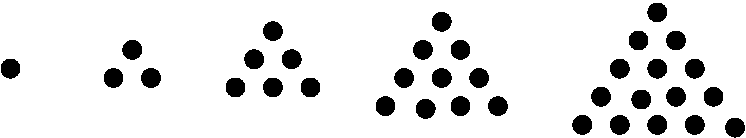
\includegraphics{./triangular_numbers.pdf}%
\end{picture}%
\setlength{\unitlength}{3947sp}%
%
\begingroup\makeatletter\ifx\SetFigFont\undefined%
\gdef\SetFigFont#1#2#3#4#5{%
  \reset@font\fontsize{#1}{#2pt}%
  \fontfamily{#3}\fontseries{#4}\fontshape{#5}%
  \selectfont}%
\fi\endgroup%
\begin{picture}(5963,1088)(1193,-2116)
\end{picture}%
 \end{center}

The first several triangular numbers are 1, 3, 6, 10, 15, et cetera.

Determine a formula for the sum of the first $n$ triangular numbers $\displaystyle \left( \sum_{i=1}^n T_i \right)$ and prove it using PMI.

\hint{The formula is $\frac{n(n+1)(n+2)}{6}$.}

\wbvfill

\workbookpagebreak

\item Consider the alternating sum of squares:
\begin{gather*}
1 \\
1 - 4 = -3 \\
1 - 4 + 9 = 6 \\
1 - 4 + 9 - 16 = -10 \\
\mbox{et cetera}
\end{gather*}
Guess a general formula for $\sum_{i=1}^n (-1)^{i-1} i^2$, and prove it using PMI.

\hint{
\begin{thm*}
\[ \forall n \in \Naturals, \; \sum_{i=1}^n (-1)^{i-1} i^2 \;= \; (-1)^{n-1} \frac{n(n+1)}{2}  \]
\end{thm*}

\begin{proof} (By mathematical induction)

{\bf Base case:} ($n=1$)
For the base case, note that when $n=1$ we have

\[\sum_{i=1}^n (-1)^{i-1} i^2 \;= \; 1 \]

\noindent and also

\[ (-1)^{n-1} \frac{n(n+1)}{2} \;= \; 1. \]

{\bf Inductive step:}

Suppose that $k>1$ is an integer such that 

\[ \sum_{i=1}^k (-1)^{i-1} i^2 \;= \; (-1)^{k-1} \frac{k(k+1)}{2}.  \]

Adding $(-1)^{k} (k+1)^2$ to both sides gives

\begin{gather*} 
\sum_{i=1}^{k+1} (-1)^{i-1} i^2 \;= \; (-1)^{k-1} \frac{k(k+1)}{2} + (-1)^{k} (k+1)^2 \\
\;= \; (-1)^{k-1} \frac{k(k+1)}{2} - (-1)^{k-1} (k+1)^2 \\ 
\;= \; (-1)^{k-1} \left( \frac{k(k+1)}{2} -  \frac{2(k+1)^2}{2} \right) \\ 
\;= \; (-1)^{k} \left( \frac{2(k+1)^2}{2} - \frac{k(k+1)}{2} \right) \\
\;= \; (-1)^{k} \frac{(k+1)(2(k+1)-k)}{2} \\
\;= \; (-1)^{k} \frac{(k+1)(k+2)}{2} \\
\end{gather*}
\end{proof}
}

\wbvfill

\workbookpagebreak

\item Prove the following formula for a product.

\[ \prod_{i=2}^n \left(1 - \frac{1}{i}\right) =  \frac{1}{n} \]

\hint{
Notice that the problem statement didn't specify the domain -- but the smallest value of $n$ that gives
a non-empty product on the left-hand side is $n=2$.  

\newpage

\begin{proof} (By mathematical induction)

{\bf Base case:} ($n=2$)
For the base case, note that when $n=2$ we have

\[ \prod_{i=2}^2 \left(1 - \frac{1}{i}\right) \quad = \quad  \left(1 - \frac{1}{2}\right) \quad = \quad 1/2 \]

\noindent and, when $n=2$, the right-hand side ($1/n$) also evaluates to $1/2$.

{\bf Inductive step:}

Suppose that $k\geq2$ is an integer such that 

\[ \prod_{i=2}^k \left(1 - \frac{1}{i}\right) =  \frac{1}{k}. \]

Then,

\begin{gather*}
\prod_{i=2}^{k+1} \left(1 - \frac{1}{i}\right) \\
= \left(1 - \frac{1}{k+1}\right) \; \cdot \; \prod_{i=2}^{k} \left(1 - \frac{1}{i}\right) \\
= \left(1 - \frac{1}{k+1}\right) \; \cdot \; \frac{1}{k} \\
= \frac{1}{k+1}.
\end{gather*}
\end{proof}

The final line skips over a tiny bit of algebraic detail.  You may feel more comfortable if you fill in those steps.

\newpage
}


\item Prove $\displaystyle \sum_{j=0}^{n}(4j+1) \; = \; 2n^{2}+3n+1$ for all
integers $n \geq 0$.

\hint{
\begin{proof} (By mathematical induction)

{\bf Base case:} ($n=0$)
For the base case, note that when $n=0$ we have

\[ \sum_{j=0}^{n}(4j+1) \; = \; (4\cdot 0 + 1 \; = \; 1 \]

\noindent also, when $n=0$,

\[ 2n^2+3n+1 \; = \; 2\cdot 0^2 +3\cdot 0 + 1 \; = \; 1. \]

{\bf Inductive step:}

Suppose that $k \geq 0$ is an integer such that 

\[  \sum_{j=0}^{k}(4j+1) \; = \; 2k^{2}+3k+1. \]

(We want to show that $\displaystyle \sum_{j=0}^{k+1}(4j+1) \; = \; 2(k+1)^{2}+3(k+1)+1$.)

So consider the sum $\displaystyle \sum_{j=0}^{k+1}(4j+1)$:

\begin{gather*}
\sum_{j=0}^{k+1}(4j+1) \\
= \; 4(k+1)+1 \; + \; \sum_{j=0}^{k}(4j+1) \\
= \;  4(k+1)+1 \; + \; 2k^{2}+3k+1 \\
= \; \rule{0pt}{18pt} \rule{2in}{0pt} \\
= \; \rule{0pt}{18pt} \rule{2in}{0pt} \\
= \; \rule{0pt}{18pt} \rule{2 in}{0pt} \\
\end{gather*}
\end{proof}


Notice that the last line given in the proof is where the inductive hypothesis gets used.  The actual last line of the proof is fairly easy to determine (hint: it is given in the "We want to show" sentence.)  So now you just have to fill in the gaps\ldots

\rule{0pt}{12pt}

}

\wbvfill

\workbookpagebreak

\item Prove $\displaystyle \sum_{i=1}^{n}\frac{1}{(2i-1)(2i+1)} \; = \; \frac{n}{2n+1}$ for all natural numbers $n$.

\hint{
\begin{proof} (By mathematical induction)

{\bf Base case:} ($n=0$)
For the base case, note that when $n=0$ 

\[ \sum_{j=0}^{n} \frac{1}{(2i-1)(2i+1)} \]

contains no terms. Thus its value is 0.

And, $\displaystyle \frac{n}{2n+1}$ also evaluates to 0 when $n=0$.

{\bf Inductive step:}

By the inductive hypothesis we may write

\[ \sum_{i=1}^{k} \frac{1}{(2i-1)(2i+1)} \; = \; \frac{k}{2k+1}. \]

Adding $\displaystyle  \frac{1}{(2(k+1)-1)(2(k+1)+1)}$ to both side of this gives

\[ \sum_{i=1}^{k+1} \frac{1}{(2i-1)(2i+1)} \; = \; \frac{k}{2k+1} \; + \; \frac{1}{(2(k+1)-1)(2(k+1)+1)}. \]

To complete the proof we must verify that 

\[ \frac{k}{2k+1} \; + \; \frac{1}{(2(k+1)-1)(2(k+1)+1)} = \frac{k+1}{2(k+1)+1}. \]

Note that
\begin{gather*}
\rule{0pt}{23pt} \frac{k}{2k+1} \; + \; \frac{1}{(2(k+1)-1)(2(k+1)+1)} \\
\rule{0pt}{23pt} = \frac{k}{2k+1} \; + \; \frac{1}{(2k+1)(2k+3)}\\
\rule{0pt}{23pt} = \frac{k(2k+3)}{(2k+1)(2k+3)} \; + \; \frac{1}{(2k+1)(2k+3)}\\
\rule{0pt}{23pt} = \frac{k(2k+3)+1}{(2k+1)(2k+3)} \\
\rule{0pt}{23pt} = \frac{2k^2+3k+1}{(2k+1)(2k+3)} \\
\rule{0pt}{23pt} = \frac{(2k+1)(k+1)}{(2k+1)(2k+3)} \\
\rule{0pt}{23pt} = \frac{k+1}{2k+3} \; = \; \frac{k+1}{2(k+1)+1}
\end{gather*}

\noindent as desired.


\end{proof}

}
\wbvfill

\workbookpagebreak

\item The \index{Fibonacci numbers} \emph{Fibonacci numbers} are a sequence of integers defined by
the rule that a number in the sequence is the sum of the two that 
precede it.

\[ F_{n+2} = F_n + F_{n+1}  \]

\noindent The first two Fibonacci numbers (actually the zeroth and the first) 
are both 1.  

\noindent Thus, the first several Fibonacci numbers are

\[ F_0 = 1, F_1=1, F_2=2, F_3=3, F_4=5, F_5=8, F_6=13, F_7=21, \; \mbox{et cetera} \]

Use mathematical induction to prove the following formula involving
Fibonacci numbers.

\[ \sum_{i=0}^n (F_i)^2 \, = \, F_n \cdot F_{n+1} \]

\hint{
\begin{proof} (by induction)

{\bf Base case:} ($n=0$)

For the base case, note that when $n=0$ 

\[ \sum_{i=0}^{n} (F_i)^2 \; = \; 1. \]

And, $\displaystyle F_n \cdot F_{n+1} \; = \; F_0 \cdot F_1 \; = \; 1 \cdot 1 \; = \; 1$. 

{\bf Inductive step:}

By the inductive hypothesis we may write

\[ \sum_{i=0}^k (F_i)^2 \; = \; F_k \cdot F_{k+1}. \]

Adding $(F_{k+1})^2$ to both sides gives

\[ \sum_{i=0}^{k+1} (F_i)^2 \; = \; F_k \cdot F_{k+1} + (F_{k+1})^2. \]

Finally, note that (using factoring and the defining property of the Fibonacci numbers)
we can show that

\begin{gather*}
 F_k \cdot F_{k+1} + (F_{k+1})^2 \\
  = \; F_{k+1} \cdot (F_k + F_{k+1}) \\
  = \; F_{k+1} \cdot F_{k+2}
\end{gather*}

So the inductive step has been proved and the result follows by PMI.
\end{proof}
}

\wbvfill

\workbookpagebreak

\end{enumerate}

%% Emacs customization
%% 
%% Local Variables: ***
%% TeX-master: "GIAM-hw.tex" ***
%% comment-column:0 ***
%% comment-start: "%% "  ***
%% comment-end:"***" ***
%% End: ***


 
\newpage

\section[Other proofs using PMI]{Divisibility statements and other proofs using PMI}

There is a very famous result known as 
\index{Fermat's little theorem}Fermat's Little Theorem.  
This would probably be abbreviated FLT except for two things.
In science fiction FLT means ``faster than light travel'' and 
there is \emph{another} theorem due to Fermat that goes by
the initials FLT: \index{Fermat's last theorem}Fermat's Last Theorem.  
Fermat's last theorem states that equations of the form $a^n+b^n=c^n$,
where $n$ is a positive natural number, 
only have integer solutions that are trivial (like $0^3+1^3=1^3$) when $n$
is greater than 2.  When $n$ is 1, there are lots of integer solutions.
When $n$ is 2, there are still plenty of integer solutions -- these are the
so-called Pythagorean triples, for example 3,4 \& 5 or 5,12 \& 13.  
It is somewhat unfair that this statement is known as Fermat's last \emph{theorem} since he didn't prove it (or at least we can't be sure that he proved it).
Five years after his death, Fermat's son published a translated\footnote{The
translation from Greek into Latin was done by Claude Bachet.} version of
Diophantus's \emph{Arithmetica} containing his father's notations.  One of
those notations -- near the place where Diophantus was discussing the
equation $x^2+y^2=z^2$ and its solution in whole numbers -- was the statement
of what is now known as Fermat's last theorem as well as the following claim:

\begin{quote}
Cuius rei demonstrationem mirabilem sane detexi hanc marginis exiguitas non caperet.
\end{quote}

In English:

\begin{quote}
I have discovered a truly remarkable proof of this that the margin of this page is too small to contain.
\end{quote}

Between 1670 and 1994 a lot of famous mathematicians worked on FLT but
never found the ``demonstrationem mirabilem.''  Finally in 1994, Andrew Wiles
of Princeton announced a proof of FLT, but in Wiles's own words, his is ``a twentieth century proof'' it can't be the proof Fermat had in mind. 

These days most people believe that Fermat was mistaken.  Probably he thought
a proof technique that works for small values of $n$ could be generalized.  
It remains a tantalizing question, can a proof of FLT using only methods
available in the 17th century be accomplished?  

Part of the reason that so many people spent so much effort on FLT
over the centuries is that Fermat had an excellent record as regards
being correct about his theorems and proofs.  The result known as Fermat's
little theorem is an example of a theorem and proof that Fermat got 
right.  It is probably known as his ``little'' theorem because its 
statement is very short, but it is actually a fairly deep result.

\begin{thm}[Fermat's Little Theorem] 
For every prime number $p$, and for all integers $x$, the $p$-th 
power of $x$ and $x$ itself are congruent mod $p$.  Symbolically:

\[ x^p \equiv x \pmod{p} \]
\end{thm}

A slight restatement of Fermat's little theorem is that $p$ is
always a divisor of $x^p-x$ (assuming $p$ is a prime and $x$ is an integer).
Math professors enjoy using their knowledge of Fermat's little theorem
to cook up divisibility results that can be proved using mathematical
induction.   For example, consider the following:

\[ \forall n \in \Naturals,  3 \divides (n^3 + 2n + 6). \]  

This is really just the $p=3$ case of Fermat's little theorem 
with a little camouflage added: $n^3 + 2n + 6 = (n^3-n)+3(n+2)$.
But let's have a look at proving this statement using PMI. 

\begin{thm} 
$\forall n \in \Naturals,  3 \divides (n^3 + 2n + 6)$
\end{thm}

\begin{proof}
(By mathematical induction)

{\bf Basis:} Clearly $3 \divides 6$.

{\bf Inductive step:} 

\noindent (We need to show that $3 \divides (k^3 + 2k + 6) \; \implies \; 3 \divides ((k+1)^3 + 2(k+1) + 6$.)

Consider the quantity $(k+1)^3 + 2(k+1) + 6$.

\begin{gather*}
   (k+1)^3 + 2(k+1) + 6 \\
 = (k^3 + 3k^2 + 3k + 1) + (2k + 2) + 6\\
 = (k^3 + 2k + 6) + 3k^2 + 3k + 3\\
 = (k^3 + 2k + 6) + 3(k^2 + k + 1).
\end{gather*}

By the inductive hypothesis, 3 is a divisor of $k^3 + 2k + 6$ so there
is an integer $m$ such that $k^3 + 2k + 6 = 3m$.
Thus,

\begin{gather*}
(k+1)^3 + 2(k+1) + 6 \\
= 3m + 3(k^2 + k + 1) \\
= 3(m + k^2 + k + 1).
\end{gather*}

This equation shows that 3 is a divisor of $(k+1)^3 + 2(k+1) + 6$, which
is the desired conclusion.
\end{proof}

\begin{exer}
Devise an inductive proof of the statement, $\forall n \in \Naturals, 5 \divides x^5+4x-10$.
\end{exer}

There is one other subtle trick for devising statements to be
proved by PMI that you should know about.  An example should 
suffice to make it clear.  Notice that $7$ is equivalent to $1 \pmod{6}$,
it follows that any power of $7$ is also $1 \pmod{6}$.  So, if we subtract
$1$ from some power of 7 we will have a number that is divisible by $6$.

The proof (by PMI) of a statement like this requires another subtle little
trick.  Somewhere along the way in the proof you'll need the identity $7=6+1$.

\begin{thm}
\[ \forall n \in \Naturals, \; 6 \divides 7^n-1 \]
\end{thm}

\begin{proof} (By PMI)

{\bf Basis:}  Note that $7^0-1$ is $0$ and also that $6 \divides 0$.

{\bf Inductive step:}  

\noindent (We need to show that if $6 \divides 7^k-1$ then $6 \divides 7^{k+1}-1$.)

\noindent Consider the quantity $7^{k+1}-1$.

\begin{gather*}
7^{k+1}-1 = 7 \cdot 7^k -1 \\
 = (6 + 1) \cdot 7^k - 1 \\
 = 6 \cdot 7^k + 1 \cdot 7^k - 1\\
 = 6(7^k) + (7^k - 1)
\end{gather*}

\noindent By the inductive hypothesis, $6 \divides 7^k - 1$ so there is
an integer $m$ such that $7^k - 1 = 6m$.  It follows that

\[ 7^{k+1}-1 = 6(7^k) + 6m. \]

So, clearly, $6$ is a divisor of $7^{k+1}-1$.

\end{proof}

Mathematical induction 
can often be used to prove inequalities.  There are quite a few examples
of families of statements where there is an inequality for every natural
number.  Often such statements seem to be \emph{obviously} true and yet 
devising a proof can be illusive.  If such is the case, try using PMI.
One hint: it is fairly typical that the inductive step in a PMI proof
of an inequality will involve reasoning that isn't particularly sharp. 
Just remember that if you have an inequality and you make the big
side even bigger, the resulting statement is certainly still true! 

Consider the sequences $2^n$ and $n!$.

\begin{center}
\begin{tabular}{c|ccccc}
$n$   & \rule{6pt}{0pt} 0 \rule{6pt}{0pt} & \rule{6pt}{0pt} 1 \rule{6pt}{0pt} &\rule{6pt}{0pt} 2 \rule{6pt}{0pt} & \rule{6pt}{0pt} 3 \rule{6pt}{0pt} & \\ \hline
$2^n$ & 1 & 2 & 4 & 8 & \\ \hline
$n!$  & 1 & 1 & 2 & 6 & \\
\end{tabular}
\end{center}

As the table illustrates, for small values of $n$, $2^n > n!$.  But from $n=4$
onward the inequality is reversed.

\begin{thm} 
\[ \forall n \geq 4 \in \Naturals, 2^n < n! \]
\end{thm}

\begin{proof} (By mathematical induction)

\noindent {\bf Basis:} When $n=4$ we have $2^4 < 4!$, which is certainly 
true ($16 < 24$).

\noindent {\bf Inductive step:} Suppose that $k$ is a natural number 
with $k > 4$, and that $2^k < k!$.  Multiply the left hand side of this
inequality by $2$ and the right hand side by $k+1$\footnote{It might be %
smoother to justify this step by first proving the lemma that %
$\forall a,b,c,d \in {\mathbb R}^+, \; a<b \land c<d \implies ac < bd$. } 
to get

\[ 2\cdot 2^{k} < (k+1) \cdot k!. \]

\noindent So

\[ 2^{k+1} < (k+1)!. \]

\end{proof}

The observant Calculus student will certainly be aware of the fact
that, asymptotically, exponential functions grow faster than polynomial
functions.  That is, if you have a base $b$ which is greater than 1, the 
function $b^x$ is eventually larger than any polynomial $p(x)$.  This
may seem a bit hard to believe if $b=1.001$ and $p(x) = 500x^{10}$.  The
graph of $y=1.001^x$ is practically indistinguishable from the line $y=1$
(at first), whereas the graph of $y=500x^{10}$ has already reached the 
astronomical value of five trillion ($5,000,000,000,000$) when $x$ is just
$10$.  Nevertheless, the exponential will eventually outstrip the polynomial.
We can use the methods of this section to get started on proving the fact 
mentioned above.  Consider the two sequences $n^2$ and $2^n$. 

\begin{center}
\begin{tabular}{c|ccccccc}
$n$   & \rule{6pt}{0pt} 0 \rule{6pt}{0pt} & \rule{6pt}{0pt} 1 \rule{6pt}{0pt} & \rule{6pt}{0pt} 2 \rule{6pt}{0pt} & \rule{6pt}{0pt} 3 \rule{6pt}{0pt} & \rule{6pt}{0pt} 4 \rule{6pt}{0pt} & \rule{6pt}{0pt} 5 \rule{6pt}{0pt} & \rule{6pt}{0pt} 6 \rule{6pt}{0pt} \\ \hline
$n^2$  & 0 & 1 & 4 & 9 & 16 & 25 & 36 \\ \hline
$2^n$ & 1 & 2 & 4 & 8 & 16 & 32 & 64 \\ 
\end{tabular}
\end{center}

If we think of a ``race'' between the sequences $n^2$ and $2^n$, notice
that $2^n$ starts out with the lead.  The two sequences are tied when 
$n=2$.  Briefly, $n^2$ goes into the lead but they are tied again when
$n=4$.  After that it would appear that $2^n$ recaptures the lead for good.
Of course we're making a rather broad presumption -- is it really true
that $n^2$ never catches up with $2^n$ again?  Well, if we're right 
then the following theorem should be provable:

\begin{thm} 
For all natural numbers $n$, if $n \geq 4$ then $n^2 \leq 2^n$.
\end{thm}
 
\begin{quote} \emph{Proof:}

\noindent {\bf Basis:} When $n=4$ we have $4^2 \leq 2^4$, which is 
true since both numbers are 16.

\noindent {\bf Inductive step:} (In the inductive step we assume
that $k^2 \leq 2^k$ and then show that $(k+1)^2 \leq 2^{k+1}$.)

The inductive hypothesis tells us that 

\[ k^2 \leq 2^k. \]

 
If we add $2k+1$ to the left-hand side of this inequality
and $2^k$ to the right-hand side we will produce the desired
inequality.  Thus our proof will follow provided that
we know that $2k+1 \leq 2^k$.  Indeed, it is sufficient to show
that $2k+1 \leq k^2$ since we already know (by the inductive
hypothesis) that $k^2 \leq 2^k$.

So the result remains in doubt unless you can complete the 
exercise that follows\ldots

\rule{0pt}{0pt} \newline \rule{0pt}{15pt} \hfill Q.E.D.??? \end{quote}


\begin{exer} 
Prove the lemma:  For all $n \in \Naturals$, if $n \geq 4$ then
$2n+1 \leq n^2$.
\end{exer}

\newpage
  
\noindent{\large \bf Exercises --- \thesection\ }


Give inductive proofs of the following 
\begin{enumerate}
\item $\forall x \in \Naturals, \; 3 \divides x^3-x$

\wbvfill

%\workbookpagebreak

\item $\forall x \in \Naturals, \; 3 \divides x^3+5x$

\wbvfill

\workbookpagebreak

\item $\forall x \in \Naturals, \; 11 \divides x^{11}+10x$

\wbvfill

%\workbookpagebreak

\item $\forall n \in \Naturals, \; 3 \divides 4^n-1$

\wbvfill

\workbookpagebreak

\item $\forall n \in \Naturals, \; 6 \divides (3n^{2}+3n-12)$

\wbvfill

%\workbookpagebreak

\item $\forall n \in \Naturals, \; 5 \divides (n^{5}-5n^{3}+14n$

\wbvfill

\workbookpagebreak

\item $\forall n \in \Naturals, \; 4 \divides (13^{n}+4n-1)$

\wbvfill

%\workbookpagebreak

\item $\forall n \in \Naturals, \; 7 \divides 8^n+6$

\wbvfill

\workbookpagebreak

\item $\forall n \in \Naturals, \; 6 \divides 2n^3 - 2n - 14$

\wbvfill

%\workbookpagebreak

\item $\forall n \geq 3 \in \Naturals, \; 3n^2+3n+1 < 2n^3$

\wbvfill

\workbookpagebreak

\item $\forall n > 3 \in \Naturals, \; n^3 < 3^n$

\wbvfill

%\workbookpagebreak

\item $\forall n \geq 3 \in \Naturals, \; n^{3}+3>n^{2}+3n+1$

\wbvfill

\workbookpagebreak

\item $\forall x \geq 4 \in \Naturals, \; x^22^x \leq 4^x$

\wbvfill

%\workbookpagebreak

\end{enumerate}


%% Emacs customization
%% 
%% Local Variables: ***
%% TeX-master: "GIAM-hw.tex" ***
%% comment-column:0 ***
%% comment-start: "%% "  ***
%% comment-end:"***" ***
%% End: ***



\newpage
 
\section{The strong form of mathematical induction}

The strong form of mathematical induction (a.k.a. the principle of
complete induction, PCI; also a.k.a. course-of-values induction) 
is so-called because the hypotheses one
uses are stronger.  Instead of showing that $P_k \implies P_{k+1}$ in
the inductive step, we get to assume that all the statements numbered
smaller than $P_{k+1}$ are true.  To make life slightly easier we'll
renumber things a little.  The statement that needs to be proved is

\[ \forall k (P_0 \land P_1 \land \ldots \land  P_{k-1}) \implies P_k. \]

 An outline of a strong inductive proof is:

\begin{center}
\begin{tabular}{|c|} \hline
\rule{16pt}{0pt}\begin{minipage}{.75\textwidth}

\rule{0pt}{16pt}{\bf \large Theorem} $ \displaystyle \forall n \in \Naturals, \; P_n $
\medskip

\rule{0pt}{20pt} {\em Proof:} (By complete induction)

\noindent {\bf Basis:}

\begin{center}
$\vdots$ \rule{36pt}{0pt} \begin{minipage}[c]{1.7 in} (Technically, a PCI %
proof doesn't require a basis.   We recommend that you show that $P_0$ %
is true anyway.) \end{minipage}
\end{center}

\noindent {\bf Inductive step:}

\begin{center}
$\vdots$ \rule{36pt}{0pt} \begin{minipage}[c]{1.7 in} (Here we must show that $\forall k,  \left( \bigwedge_{i=0}^{k-1} P_i \right) \implies P_{k}$ is true.) \end{minipage}
\end{center}

\rule{0pt}{0pt} \hspace{\fill} Q.E.D. \rule[-10pt]{0pt}{16pt}
\end{minipage} \rule{16pt}{0pt} \\ \hline
\end{tabular}
\end{center}
\medskip

It's fairly common that we won't truly need all of the statements from $P_0$
to $P_{k-1}$ to be true, but just one of them (and we don't know {\em a priori} 
which one).  The following is a classic result; the proof that all numbers
greater than 1 have prime factors.

\begin{thm} For all natural numbers $n$, $n > 1$ implies $n$ has a prime 
factor.
\end{thm}

\begin{proof} (By strong induction)
Consider an arbitrary natural number $n>1$.  If $n$ is prime then $n$ clearly
has a prime factor (itself), so suppose that $n$ is not prime.  By 
definition, a composite
natural number can be factored, so $n=a \cdot b$ for some pair of natural
numbers $a$ and $b$ which are both greater than 1.  Since $a$ and $b$ are  
factors of $n$ both greater than 1, it follows that $a < n$ (it is also 
true that $b < n$ but we don't need that \ldots).  The inductive hypothesis
can now be applied to deduce that $a$ has a prime factor $p$.  Since
$p \divides a$ and $a \divides n$, by transitivity $p \divides n$.  Thus
$n$ has a prime factor.
\end{proof}
  

\newpage

\noindent{\large \bf Exercises --- \thesection\ }


Give inductive proofs of the following 
\begin{enumerate}
\item A ``postage stamp problem'' is a problem that (typically) asks
us to determine what total postage values can be produced using two
sorts of stamps.  Suppose that you have $3$\cents\  stamps and $7$\cents\ 
stamps, show (using strong induction) that any postage value $12$\cents\ 
or higher can be achieved.  That is, 

\[ \forall n \in \Naturals, n \geq 12 \; \implies \;
\exists x,y \in \Naturals , n = 3x + 7y. \]
 
 \wbvfill

\workbookpagebreak

\item Show that any integer postage of $12 \cents$ or more can be made using
only $4\cents$ and $5\cents$ stamps.

\wbvfill

%\workbookpagebreak

\item The polynomial equation $x^2 = x+1$ has two solutions, 
$\alpha = \frac{1+\sqrt{5}}{2}$ and $\beta = \frac{1-\sqrt{5}}{2}$.
Show that the Fibonacci number $F_n$ is less than or equal to $\alpha^{n}$
for all $n \geq 0$.

\wbvfill

\workbookpagebreak

\end{enumerate}


%% Emacs customization
%% 
%% Local Variables: ***
%% TeX-master: "GIAM-hw.tex" ***
%% comment-column:0 ***
%% comment-start: "%% "  ***
%% comment-end:"***" ***
%% End: ***




%% Emacs customization
%% 
%% Local Variables: ***
%% TeX-master: "GIAM.tex" ***
%% comment-column:0 ***
%% comment-start: "%% "  ***
%% comment-end:"***" ***
%% End: ***



\chapter{Relations and functions}
\label{ch:rel}

{\em If evolution really works, how come mothers only have two hands? --Milton Berle}



\section{Relations}

A \emph{relation} in mathematics is a symbol that can be placed between
two numbers (or variables) to create a logical statement (or open sentence).
The main point here is that the insertion of a relation symbol between 
two numbers creates a statement whose value is either true or false.
For example, we have previously seen the divisibility symbol ($\mid$) and noted
the common error of mistaking it for the division symbol ($/$); one of these
tells us to perform an arithmetic operation, the other asks us whether 
\emph{if} such an operation were performed there would be a remainder.  
There are many other symbols that we have seen which have this characteristic,
the most important is probably $=$, but there are lots: $\neq$, $<$, $\leq$, 
$>$, $\geq$ all work this way -- if we place them between two numbers
we get a Boolean thing, it's either true or false.  If, instead of numbers, 
we think of placing sets on either side of a relation symbol, then
 $=$, $\subseteq$  and $\supseteq$ are valid relation symbols. If we think 
of placing logical expressions on either side of a relation then, 
honestly, \emph{any} of the logical symbols is a relation, but we normally
think of $\land$ and $\lor$ as operators and give things like $\equiv$, 
$\implies$ and $\iff$ the status of relations. 

In the examples we've looked at the things on either side of a relation
are of the same type.  This is usually, but not always, the case.  The 
prevalence of relations with the same kind of things being compared has
even lead to the aphorism ``Don't compare apples and oranges.''  Think 
about the symbol $\in$ for a moment.  As we've seen previously, it
isn't usually appropriate to put \emph{sets} on either side of this,
we might have numbers or other objects on the left and sets on the right.
Let's look at a small example.  Let $A = \{1,2,3,a,b\}$ and let 
$B=\{ \{1,2,a\}, \{1,3,5,7,\ldots\}, \{1\} \}$.  The ``element of'' 
relation, $\in$, is a \emph{relation from $A$ to $B$}.  

\begin{figure}[!hbtp]
\begin{picture}(0,0)%
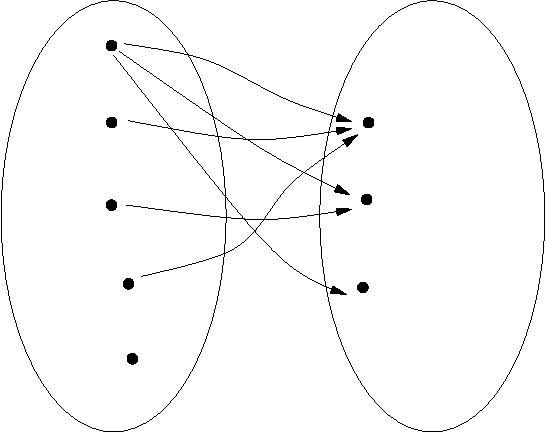
\includegraphics{figures/first_relation.pdf}%
\end{picture}%
\setlength{\unitlength}{3947sp}%
%
\begingroup\makeatletter\ifx\SetFigFont\undefined%
\gdef\SetFigFont#1#2#3#4#5{%
  \reset@font\fontsize{#1}{#2pt}%
  \fontfamily{#3}\fontseries{#4}\fontshape{#5}%
  \selectfont}%
\fi\endgroup%
\begin{picture}(4366,3466)(1193,-3819)
\put(1876,-811){\makebox(0,0)[lb]{\smash{{\SetFigFont{12}{14.4}{\familydefault}{\mddefault}{\updefault}{\color[rgb]{0,0,0}1}%
}}}}
\put(2026,-3286){\makebox(0,0)[lb]{\smash{{\SetFigFont{12}{14.4}{\familydefault}{\mddefault}{\updefault}{\color[rgb]{0,0,0}b}%
}}}}
\put(4276,-2011){\makebox(0,0)[lb]{\smash{{\SetFigFont{12}{14.4}{\familydefault}{\mddefault}{\updefault}{\color[rgb]{0,0,0}$\{1,3,5,7,\ldots\}$}%
}}}}
\put(4276,-1411){\makebox(0,0)[lb]{\smash{{\SetFigFont{12}{14.4}{\familydefault}{\mddefault}{\updefault}{\color[rgb]{0,0,0}$\{1,2,a\}$}%
}}}}
\put(4276,-2686){\makebox(0,0)[lb]{\smash{{\SetFigFont{12}{14.4}{\familydefault}{\mddefault}{\updefault}{\color[rgb]{0,0,0}$\{1\}$}%
}}}}
\put(2026,-2686){\makebox(0,0)[lb]{\smash{{\SetFigFont{12}{14.4}{\familydefault}{\mddefault}{\updefault}{\color[rgb]{0,0,0}a}%
}}}}
\put(1876,-1411){\makebox(0,0)[lb]{\smash{{\SetFigFont{12}{14.4}{\familydefault}{\mddefault}{\updefault}{\color[rgb]{0,0,0}2}%
}}}}
\put(1876,-2086){\makebox(0,0)[lb]{\smash{{\SetFigFont{12}{14.4}{\familydefault}{\mddefault}{\updefault}{\color[rgb]{0,0,0}3}%
}}}}
\end{picture}%

\caption[An example of a relation.]{The ``element of'' relation %
is an example of a relation that goes \emph{from} one set \emph{to} a %
different set.}
\label{fig:rel1} 
\end{figure}

A diagram such as we have given in Figure~\ref{fig:rel1} seems like a 
very natural thing.  Such pictures certainly give us an easy visual 
tool for thinking
about relations.  But we should point out certain hidden assumptions.
First, they'll only work if we are dealing with finite sets, or sets
like the odd numbers in our example (sets that are infinite but could
in principle be listed).  Second, by drawing the two sets separately,
it seems that we are assuming they are not only different, but 
\emph{disjoint}.  The sets not only need not be disjoint, but often
(most of the time!) we have relations that go from a set to itself
so the sets in a picture like this may be identical.  In Figure~\ref{fig:rel2}
we illustrate the divisibility relation on the set of all divisors of
6 --- this is an example in which the sets on either side of the relation
are the same.  Notice the linguistic distinction, we can talk about
either ``a relation from $A$ to $B$'' (when there are really two 
different sets) or ``a relation on $A$'' (when there is only one). 

\begin{figure}[!hbtp]
\begin{picture}(0,0)%
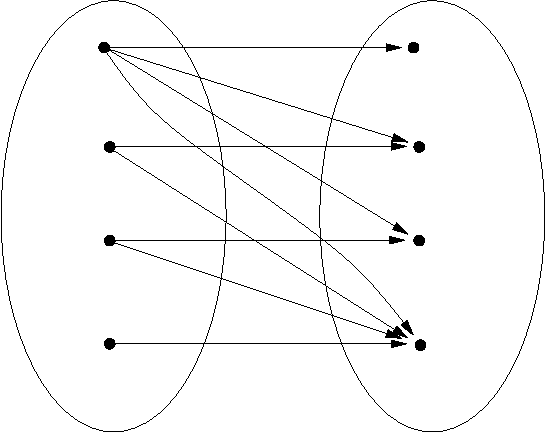
\includegraphics{./2nd_relation.pdf}%
\end{picture}%
\setlength{\unitlength}{3947sp}%
%
\begingroup\makeatletter\ifx\SetFigFont\undefined%
\gdef\SetFigFont#1#2#3#4#5{%
  \reset@font\fontsize{#1}{#2pt}%
  \fontfamily{#3}\fontseries{#4}\fontshape{#5}%
  \selectfont}%
\fi\endgroup%
\begin{picture}(4366,3466)(1193,-3819)
\put(1876,-3136){\makebox(0,0)[lb]{\smash{{\SetFigFont{12}{14.4}{\familydefault}{\mddefault}{\updefault}{\color[rgb]{0,0,0}6}%
}}}}
\put(1876,-2311){\makebox(0,0)[lb]{\smash{{\SetFigFont{12}{14.4}{\familydefault}{\mddefault}{\updefault}{\color[rgb]{0,0,0}3}%
}}}}
\put(1876,-1561){\makebox(0,0)[lb]{\smash{{\SetFigFont{12}{14.4}{\familydefault}{\mddefault}{\updefault}{\color[rgb]{0,0,0}2}%
}}}}
\put(1858,-763){\makebox(0,0)[lb]{\smash{{\SetFigFont{12}{14.4}{\familydefault}{\mddefault}{\updefault}{\color[rgb]{0,0,0}1}%
}}}}
\put(4678,-2302){\makebox(0,0)[lb]{\smash{{\SetFigFont{12}{14.4}{\familydefault}{\mddefault}{\updefault}{\color[rgb]{0,0,0}3}%
}}}}
\put(4678,-1548){\makebox(0,0)[lb]{\smash{{\SetFigFont{12}{14.4}{\familydefault}{\mddefault}{\updefault}{\color[rgb]{0,0,0}2}%
}}}}
\put(4637,-762){\makebox(0,0)[lb]{\smash{{\SetFigFont{12}{14.4}{\familydefault}{\mddefault}{\updefault}{\color[rgb]{0,0,0}1}%
}}}}
\put(4692,-3127){\makebox(0,0)[lb]{\smash{{\SetFigFont{12}{14.4}{\familydefault}{\mddefault}{\updefault}{\color[rgb]{0,0,0}6}%
}}}}
\end{picture}%

\caption[An example of the ``divides'' relation.]{The ``divides'' relation %
is an example of a relation that goes from a set to itself.  In this example %
we say that we have a relation \emph{on} the set of divisors of 6.}
\label{fig:rel2} 
\end{figure}
 
Purists will note that it is really inappropriate to represent the same set
in two different places in a Venn diagram.  The diagram in Figure~\ref{fig:rel2}
should really look like this:

\begin{center}
\begin{picture}(0,0)%
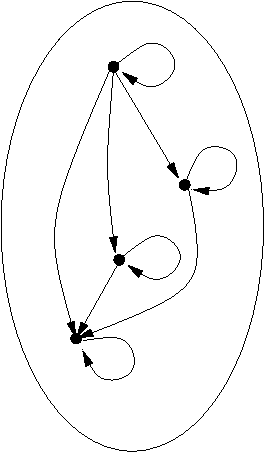
\includegraphics{figures/2nd_relation_v2.pdf}%
\end{picture}%
\setlength{\unitlength}{3947sp}%
%
\begingroup\makeatletter\ifx\SetFigFont\undefined%
\gdef\SetFigFont#1#2#3#4#5{%
  \reset@font\fontsize{#1}{#2pt}%
  \fontfamily{#3}\fontseries{#4}\fontshape{#5}%
  \selectfont}%
\fi\endgroup%
\begin{picture}(2116,3614)(1118,-3818)
\put(1876,-2311){\makebox(0,0)[lb]{\smash{{\SetFigFont{12}{14.4}{\familydefault}{\mddefault}{\updefault}{\color[rgb]{0,0,0}3}%
}}}}
\put(1858,-763){\makebox(0,0)[lb]{\smash{{\SetFigFont{12}{14.4}{\familydefault}{\mddefault}{\updefault}{\color[rgb]{0,0,0}1}%
}}}}
\put(1501,-2986){\makebox(0,0)[lb]{\smash{{\SetFigFont{12}{14.4}{\familydefault}{\mddefault}{\updefault}{\color[rgb]{0,0,0}6}%
}}}}
\put(2326,-1786){\makebox(0,0)[lb]{\smash{{\SetFigFont{12}{14.4}{\familydefault}{\mddefault}{\updefault}{\color[rgb]{0,0,0}2}%
}}}}
\end{picture}%

\end{center}

Indeed, this representation is definitely preferable, although it may be more crowded.  
A picture such as this is
known as the \index{directed graph}\emph{directed graph} (a.k.a. \index{digraph}\emph{digraph})
of the relation.

Recall that when we were discussing sets we said the best way to describe 
a set is simply to list all of its elements.  Well, what is the best
way to describe a relation?  In the same spirit, it would seem we should
explicitly list all the things that make the relation true.  But it takes
a \emph{pair} of things, one to go on the left side and one to go on the 
right, to make a relation true (or for that matter false!).  Also it should 
be evident that order is important in this context, for example $2<3$ is true
but $3<2$ isn't.  The identity of a relation is so intimately tied up with
the set of ordered pairs that make it true, that when dealing with abstract
relations we \emph{define them} as sets of ordered pairs.

Given two sets, $A$ and $B$, the \index{Cartesian product}
\emph{Cartesian product of $A$ and $B$} 
is the set of all ordered pairs $(a,b)$ where $a$ is in $A$ and $b$ is in $B$.
We denote the Cartesian product using the symbol $\times$.  

\[ A \times B = \{ (a,b) \suchthat a \in A \land b \in B \} \]

\noindent From here on out
in your mathematical career you'll need to take note of the context that
the symbol $\times$ appears in.  If it appears between numbers go ahead and
multiply, but if it appears between sets you're doing something different --
forming the Cartesian product.

The familiar $x$--$y$ plane, is often called the Cartesian plane.  This
is done for two reasons. \index{Descartes, Rene}Rene Descartes, the famous
mathematician and philosopher, was the first to consider coordinatizing
the plane and thus is responsible for our current understanding of the
relationship between geometry and algebra.  Rene Descartes' name is also
memorialized in the definition of the Cartesian product of sets, and the
plane is nothing more than the product $\Reals \times \Reals$.  Indeed,
the plane provided the very first example of the concept that was later
generalized to the Cartesian product of sets.

\begin{exer}
Suppose $A = \{1,2,3\}$ and $B = \{a,b,c\}$.  Is $(a,1)$ in the Cartesian
product $A \times B$?  List all elements of $A \times B$.
\end{exer} 

In the abstract, we can define a relation as \emph{any} subset of an
appropriate Cartesian product.  So an abstract relation $\relR$ from a set 
$A$ to a set $B$ is just some subset of $A \times B$.  Similarly, a
relation $\relR$ on a set $S$ is defined by a subset of $S \times S$.
This definition looks a little bit strange when we apply it to an
actual (concrete) relation that we already know about.  Consider the
relation ``less than.''   To describe ``less than'' as a subset of
a Cartesian product we must write

\[ < \; = \; \{ (x,y) \in \Reals \times \Reals \suchthat y-x \in \Reals^+ \}.\] 
\noindent This looks funny.

Also, if we have defined some relation $\relR \subseteq A \times B$, then in order
to say that a particular pair, $(a,b)$, of things make the relation true we
have to write 

\[ a\relR b. \]

\noindent This looks funny too.  

Despite the strange appearances, these 
examples do express the correct way to deal with relations.

Let's do a completely made-up example.  Suppose $A$ is the set
$\{a,e,i,o,u\}$ and $B$ is the set $\{r,s,t,l,n\}$ and we define 
a relation from $A$ to $B$ by

\[ \relR = \{ (a,s), (a,t), (a,n), (e,t), (e,l), (e,n), (i,s), (i,t), (o,r), (o,n), (u,s) \}. \]

Then, for example, because $(e,t) \in \relR$ we can write $e \relR t$.  We indicate the
negation of the concept that two elements are related by drawing a slash 
through the name of the relation, for example the notation $\neq$ is certainly
familiar to you, as is $\nless$ (although in this latter case we 
would normally write $\geq$ instead).  We can denote the fact that
$(a,l)$ is not a pair that makes the relation true by writing $a \nrelR l$.

We should mention another way of visualizing
relations.  When we are dealing with a relation on $\Reals$, the
relation is actually a subset of $\Reals \times \Reals$, that means 
we can view the relation as a subset of the $x$--$y$ plane.  In other 
words, we can graph it.  The graph of the ``$<$'' relation is
given in Figure~\ref{fig:lt_graph}.

\begin{figure}[!hbtp]
\begin{center}
\begin{picture}(0,0)%
\includegraphics{figures/less_than_on_RxR.pdf}%
\end{picture}%
\setlength{\unitlength}{3947sp}%
%
\begingroup\makeatletter\ifx\SetFigFont\undefined%
\gdef\SetFigFont#1#2#3#4#5{%
  \reset@font\fontsize{#1}{#2pt}%
  \fontfamily{#3}\fontseries{#4}\fontshape{#5}%
  \selectfont}%
\fi\endgroup%
\begin{picture}(3324,3324)(1189,-3673)
\end{picture}%

\end{center}
\caption[The graph of the ``less than'' relation.]{The ``less than'' relation %
can be viewed as a subset of $\Reals \times \Reals$, i.e. it can be graphed.}
\label{fig:lt_graph} 
\end{figure}
  
A relation on any set that is a subset of $\Reals$ can likewise be
graphed.  The graph of the ``$\mid$'' relation is
given in Figure~\ref{fig:div_graph}.

\begin{figure}[!hbtp]
\begin{center}
\begin{picture}(0,0)%
\includegraphics{figures/divides_on_NxN.pdf}%
\end{picture}%
\setlength{\unitlength}{3947sp}%
%
\begingroup\makeatletter\ifx\SetFigFont\undefined%
\gdef\SetFigFont#1#2#3#4#5{%
  \reset@font\fontsize{#1}{#2pt}%
  \fontfamily{#3}\fontseries{#4}\fontshape{#5}%
  \selectfont}%
\fi\endgroup%
\begin{picture}(3324,3324)(1189,-3673)
\end{picture}%

\end{center}
\caption[The graph of the divisibility relation.]{The divisibility relation %
can be graphed.  Only those points (as indicated) with integer coordinates %
are in the graph.}
\label{fig:div_graph} 
\end{figure}
 
Eventually, we will get around to defining functions as relations that
have a certain nice property.  For the moment, we'll just note that
some of the operations that you are used to using with functions
also apply with relations.  When one function ``undoes'' what another
function ``does'' we say the functions are inverses.  For example,
the function $f(x)=2x$ (i.e. doubling) and the function $g(x)=x/2$ (halving)
are inverse functions because, no matter what number we start with, if we
double it and then halve that result, we end up with the original number.
The \index{inverse, of a relation}inverse of a relation $\relR$ is written $\relR^{-1}$ and it consists of
the reversals of the pairs in $\relR$,

\[ \relR^{-1} = \{ (b,a) \suchthat (a,b) \in \relR \}. \]

This can also be expressed by writing

\[ b\relR^{-1}a \; \iff \; a\relR b. \]

The process of ``doing one function and then doing another'' is known
as \index{composition, of functions}functional composition.  For instance,
if $f(x) = 2x+1$ and $g(x) = \sqrt{x}$, then we can compose them (in two
different orders) to obtain either $f(g(x)) = 2\sqrt{x}+1$ or 
$g(f(x)) = \sqrt{2x+1}$.  When composing functions there is an ``intermediate
result'' that you get by applying the first function to your input, and then
you calculate the second function's value at the intermediate result.  
(For example, in calculating $g(f(4))$ we get the intermediate result
$f(4) = 9$ and then we go on to calculate $g(9) = 3$.)

The definition of the \index{composition, of relations}\emph{composite}
of two relations focuses very much on this idea
of the intermediate result.  Suppose $\relR$ is a relation from
$A$ to $B$ and $\relS$ is a relation from $B$ to $C$ then the composite
$\relS \circ \relR$ is given by

\[  \relS \circ \relR \; = \; \{ (a,c) \suchthat \exists b \in B, (a,b) \in \relR \, \land (b,c) \in \relS \}. \]

In this definition, $b$ is the ``intermediate result,'' if there is no such
$b$ that serves to connect $a$ to $c$ then $(a,c)$ won't be in the composite.
Also, notice that this is the composition $\relR$ first, then $\relS$, but
it is written as $\relS \circ \relR$  -- watch out for this!  The 
compositions of relations should be read from right to left.  This convention
makes sense when you consider functional composition, $f(g(x))$ means $g$ 
first, then $f$ so if we use the ``little circle'' notation for the
composition of relations we have $f \circ g (x) = f(g(x))$ which is nice
because the symbols $f$ and $g$ appear in the same order.  But beware! there
are atavists out there who write their compositions the other way around.

 
You should probably have a diagram like the following in mind while thinking
about the composition of relations.  Here, we have the set $A=\{1,2,3,4\}$,
the set $B$ is $\{a,b,c,d\}$ and $C=\{w,x,y,z\}$.  The relation
$\relR$ goes from $A$ to $B$ and consists of the following set of pairs,

\[ \relR \; = \; \{(1,a), (1,c), (2,d), (3,c), (3,d) \}. \]

And 

\[ \relS \; = \; \{(a,y), (b,w), (b,x), (b,z) \}. \]

\vfill

\begin{picture}(0,0)%
\includegraphics{./composite_relation.pdf}%
\end{picture}%
\setlength{\unitlength}{3947sp}%
%
\begingroup\makeatletter\ifx\SetFigFont\undefined%
\gdef\SetFigFont#1#2#3#4#5{%
  \reset@font\fontsize{#1}{#2pt}%
  \fontfamily{#3}\fontseries{#4}\fontshape{#5}%
  \selectfont}%
\fi\endgroup%
\begin{picture}(6241,3767)(1193,-3819)
\put(1876,-2311){\makebox(0,0)[lb]{\smash{{\SetFigFont{12}{14.4}{\familydefault}{\mddefault}{\updefault}{\color[rgb]{0,0,0}3}%
}}}}
\put(1876,-1561){\makebox(0,0)[lb]{\smash{{\SetFigFont{12}{14.4}{\familydefault}{\mddefault}{\updefault}{\color[rgb]{0,0,0}2}%
}}}}
\put(1858,-763){\makebox(0,0)[lb]{\smash{{\SetFigFont{12}{14.4}{\familydefault}{\mddefault}{\updefault}{\color[rgb]{0,0,0}1}%
}}}}
\put(1876,-3136){\makebox(0,0)[lb]{\smash{{\SetFigFont{12}{14.4}{\familydefault}{\mddefault}{\updefault}{\color[rgb]{0,0,0}4}%
}}}}
\put(3001,-286){\makebox(0,0)[lb]{\smash{{\SetFigFont{12}{14.4}{\familydefault}{\mddefault}{\updefault}{\color[rgb]{0,0,0}$\relR$}%
}}}}
\put(5701,-211){\makebox(0,0)[lb]{\smash{{\SetFigFont{12}{14.4}{\familydefault}{\mddefault}{\updefault}{\color[rgb]{0,0,0}$\relS$}%
}}}}
\put(4276,-3061){\makebox(0,0)[lb]{\smash{{\SetFigFont{12}{14.4}{\familydefault}{\mddefault}{\updefault}{\color[rgb]{0,0,0}d}%
}}}}
\put(4276,-661){\makebox(0,0)[lb]{\smash{{\SetFigFont{12}{14.4}{\familydefault}{\mddefault}{\updefault}{\color[rgb]{0,0,0}a}%
}}}}
\put(4276,-1486){\makebox(0,0)[lb]{\smash{{\SetFigFont{12}{14.4}{\familydefault}{\mddefault}{\updefault}{\color[rgb]{0,0,0}b}%
}}}}
\put(4276,-2161){\makebox(0,0)[lb]{\smash{{\SetFigFont{12}{14.4}{\familydefault}{\mddefault}{\updefault}{\color[rgb]{0,0,0}c}%
}}}}
\put(6676,-736){\makebox(0,0)[lb]{\smash{{\SetFigFont{12}{14.4}{\familydefault}{\mddefault}{\updefault}{\color[rgb]{0,0,0}w}%
}}}}
\put(6676,-1486){\makebox(0,0)[lb]{\smash{{\SetFigFont{12}{14.4}{\familydefault}{\mddefault}{\updefault}{\color[rgb]{0,0,0}x}%
}}}}
\put(6676,-2236){\makebox(0,0)[lb]{\smash{{\SetFigFont{12}{14.4}{\familydefault}{\mddefault}{\updefault}{\color[rgb]{0,0,0}y}%
}}}}
\put(6676,-3061){\makebox(0,0)[lb]{\smash{{\SetFigFont{12}{14.4}{\familydefault}{\mddefault}{\updefault}{\color[rgb]{0,0,0}z}%
}}}}
\end{picture}%


\begin{exer}
Notice that the composition $\relR \circ \relS$ is impossible (or, more
properly, it is empty).  Why?

What is the (only) pair in the composition $\relS \circ \relR$ ?
\end{exer}

\newpage

\noindent{\large \bf Exercises --- \thesection\ }

\begin{enumerate}
\item The \index{lexicographic order}\emph{lexicographic order}, 
$<_{\mbox{lex}}$, is a relation on the
set of all words, where $x <_{\mbox{lex}} y$ means that $x$ would come before
$y$ in the dictionary.  Consider just the three letter words like ``iff'',
``fig'', ``the'', et cetera.  Come up with a usable definition for
$x_1x_2x_3  <_{\mbox{lex}} y_1y_2y_3$.

\item What is the graph of ``$=$'' in $\Reals \times \Reals$?

\item The \index{inverse relation} \emph{inverse} of a relation $\relR$
is denoted $\relR^{-1}$.  It contains exactly the same ordered pairs
as $\relR$ but with the order switched.  (So technically, they aren't
\emph{exactly} the same ordered pairs \ldots)

\[ \relR^{-1} = \{ (b,a) \suchthat (a,b) \in \relR \} \]

\noindent Define a relation $\relS$ on $\Reals \times \Reals$ by
$\relS = \{ (x,y) \suchthat y = \sin x \}$.  What is $\relS^{-1}$?
Draw a single graph containing $\relS$ and $\relS^{-1}$.

\item The ``socks and shoes'' rule is a very silly little mnemonic
for remembering how to invert a composition.  If we think of undoing
the process of putting on our socks and shoes (that's socks first, then
shoes) we have to first remove our shoes, \emph{then} take off our socks.

The socks and shoes rule is valid for relations as well.

Prove that $(\relS \circ \relR)^{-1} = \relR^{-1} \circ \relS^{-1}$.

\end{enumerate} 

%% Emacs customization
%% 
%% Local Variables: ***
%% TeX-master: "GIAM-hw.tex" ***
%% comment-column:0 ***
%% comment-start: "%% "  ***
%% comment-end:"***" ***
%% End: ***



\newpage

\section{Properties of relations}

There are two special classes of relations that we will study
in the next two sections, equivalence relations and ordering relations.
The prototype for an equivalence relation is the ordinary notion
of numerical equality, $=$.  The prototypical ordering relation
is $\leq$.  Each of these has certain salient properties that are the
root causes of their importance.  In this section we will study a 
compendium of properties that a relation may or may not have.  

A relation that has three of the properties we'll discuss:

\begin{enumerate}
\item \index{reflexivity} reflexivity 
\item \index{symmetry}symmetry 
\item \index{transitivity}transitivity
\end{enumerate}

\noindent is said to be an equivalence relation; it will in some ways resemble
$=$.

A relation that has another set of three properties:

\begin{enumerate}
\item \index{reflexivity}reflexivity 
\item \index{anti-symmetry}anti-symmetry 
\item \index{transitivity}transitivity
\end{enumerate}

\noindent is called an ordering relation; it will resemble $\leq$.

Additionally, there is a property known as irreflexivity that many
relations have.

There are a total of 5 properties that we have named, and we will discuss
them all more thoroughly.  But first, we'll state the formal definitions.
Take note that these properties are all stated for a relation that goes
from a set to itself, indeed, most of them wouldn't even make sense if
we tried to define them for a relation from a set to a different set.

\clearpage

\begin{table}[hbt] 
\begin{center}
\begin{tabular}{|c|} \hline
\begin{minipage}{.95\textwidth} \centerline{\rule{0pt}{15pt} A relation $\relR$ on a set $S$ is {\bf reflexive} iff} 
\rule{0pt}{15pt} \centerline{ $\displaystyle \forall a \in S, \quad a \relR a $} 
\rule[-6pt]{0pt}{21pt} ``Everything is related to itself.''
\end{minipage} \\ \hline
\begin{minipage}{.95\textwidth} \centerline{\rule{0pt}{15pt}A relation $\relR$ on a set $S$ is {\bf irreflexive} iff}
\rule{0pt}{15pt} \centerline{ $\displaystyle \forall a \in S, \quad a \nrelR a $ }
\rule[-6pt]{0pt}{21pt} ``Nothing is related to itself.''
\end{minipage} \\ \hline
\begin{minipage}{.95\textwidth} \centerline{\rule{0pt}{15pt}A relation $\relR$ on a set $S$ is {\bf symmetric} iff}
\rule{0pt}{15pt} \centerline{ $\displaystyle \forall a,b \in S, \quad a \relR b \; \implies \; b \relR a $ }
\rule[-6pt]{0pt}{21pt} ``No one-way streets.'' 
\end{minipage} \\ \hline
\begin{minipage}{.95\textwidth} \centerline{\rule{0pt}{15pt}A relation $\relR$ on a set $S$ is {\bf anti-symmetric} iff}
\rule{0pt}{15pt} \centerline{ $\displaystyle \forall a,b \in S, \quad a \relR b \; \land b \relR a \quad \implies \quad a=b $}
\rule[-6pt]{0pt}{21pt} ``Only one-way streets.''
\end{minipage} \\ \hline
\begin{minipage}{.95\textwidth} \centerline{\rule{0pt}{15pt}A relation $\relR$ on a set $S$ is {\bf transitive} iff}
\rule{0pt}{15pt} \centerline{ $\displaystyle \forall a,b,c \in S, \quad a \relR b \; \land \; b \relR c \quad \implies \quad a \relR c$ }
\rule[-6pt]{0pt}{21pt} ``Whenever there's a roundabout route, there's a direct route.''
\end{minipage} \\ \hline
\end{tabular} 
\end{center} 
\caption[Properties of relations.]{Properties that relations may (or may not) have.}
\index{Properties of relations}
\label{tab:rel_props}
\end{table}


The digraph of a relation that is reflexive will have little loops at every vertex.
The digraph of a relation that is irreflexive will contain no loops at all.
Hopefully it is clear that these concepts represent extreme opposite possibilities --
they are \emph{not} however negations of one another.

\begin{exer}
Find the logical denial of the property that says a relation is reflexive

\[ {\lnot}(\forall a \in S, \quad a \relR a). \]

How does this differ from the defining property for ``irreflexive''?
\end{exer}

If a relation $\relR$ is defined on some subset $S$ of the reals, then it can be graphed
in the Euclidean plane.  Reflexivity for $\relR$ can be interpreted in terms of the line
$L$ defined by the equation $y=x$.  Every point in $(S \times S) \cap L$
must be in $\relR$.  A similar statement can be made concerning the irreflexive property.
If a relation $\relR$ is irreflexive its graph completely avoids the line $y=x$.

Note that the reflexive and irreflexive properties are defined with a single quantified
variable.  Symmetry and anti-symmetry require two universally quantified variables for
their definitions.

\begin{quote}
A relation $\relR$ on a set $S$ is {\bf symmetric} iff
\[ \forall a,b \in S, \quad a \relR b \; \implies \; b \relR a. \] 
\end{quote}

\noindent This can be interpreted in terms of digraphs as follows:  If a connection
from $a$ to $b$ exists in the digraph of $\relR$, then there must also be a connection
from $b$ to $a$.   In Table~\ref{tab:rel_props} this is interpreted as ``no one-way streets''
and while that's not quite what it says, that \emph{is} the effect of this definition.
Since \emph{if} a connection exists in one direction, there must also be a connection 
in the other direction, it follows that we will never see a one-way connection.

Because most of the properties we are studying are defined using conditional statements
it is often the case that a relation has a property for vacuous reasons.  When the ``if'' part
doesn't happen, there's no need for its corresponding ``then'' part to happen either -- the 
conditional is still true.  In the context of our discussion on the symmetry property of
a relation this means that the following digraph \emph{is} the digraph of a symmetric
relation (although it is neither reflexive nor irreflexive).

\begin{center}
\begin{picture}(0,0)%
\includegraphics{./vacuously_symmetric.pdf}%
\end{picture}%
\setlength{\unitlength}{3947sp}%
%
\begingroup\makeatletter\ifx\SetFigFont\undefined%
\gdef\SetFigFont#1#2#3#4#5{%
  \reset@font\fontsize{#1}{#2pt}%
  \fontfamily{#3}\fontseries{#4}\fontshape{#5}%
  \selectfont}%
\fi\endgroup%
\begin{picture}(3606,1822)(1653,-1801)
\put(1824,-774){\makebox(0,0)[lb]{\smash{{\SetFigFont{12}{14.4}{\familydefault}{\mddefault}{\updefault}{\color[rgb]{0,0,0}a}%
}}}}
\put(2701,-1186){\makebox(0,0)[lb]{\smash{{\SetFigFont{12}{14.4}{\familydefault}{\mddefault}{\updefault}{\color[rgb]{0,0,0}b}%
}}}}
\put(3376,-511){\makebox(0,0)[lb]{\smash{{\SetFigFont{12}{14.4}{\familydefault}{\mddefault}{\updefault}{\color[rgb]{0,0,0}c}%
}}}}
\put(4276,-1036){\makebox(0,0)[lb]{\smash{{\SetFigFont{12}{14.4}{\familydefault}{\mddefault}{\updefault}{\color[rgb]{0,0,0}d}%
}}}}
\end{picture}%

\end{center}

Anti-symmetry is described as meaning ``only one-way streets'' but the definition is given
as:

\begin{quote}
A relation $\relR$ on a set $S$ is {\bf anti-symmetric} iff \newline
\centerline{ $\displaystyle \forall a,b \in S, \quad a \relR b \; \land b \relR a \quad \implies \quad a=b$.}
\end{quote}

It may be hard at first to understand why the definition we use for anti-symmetry is the one above.
If one wanted to insure that there were never two-way connections between elements of the set it
might seem easier to define anti-symmetry as follows:

\begin{quote}
(Alternate definition) A relation $\relR$ on a set $S$ is {\bf anti-symmetric} iff \newline
\centerline{ $\displaystyle \forall a,b \in S, \quad a \relR b \; \implies \; b \nrelR a$.}
\end{quote}

This definition may seem more straight-forward, but it turns out the original definition is
easier to use in proofs.  We need to convince ourselves that the (first) definition really
accomplishes what we want.  Namely, if a relation $\relR$ satisfies the property that
$\displaystyle \forall a,b \in S, \quad a \relR b \; \land \; b \relR a \quad \implies \quad a=b$,
then there will not actually be any pair of elements that are related in both orders.  One
way to think about it is this: suppose that $a$ and $b$ are distinct elements of $S$ and
that both $a \relR b$ and $b \relR a$ are true.  The property now guarantees that $a=b$
which contradicts the notion that $a$ and $b$ are distinct.  This is a miniature proof
by contradiction; if you assume there \emph{are} a pair of distinct elements that are
related in both orders you get a contradiction, so there \emph{aren't}!

A funny thing about the anti-symmetry property is this:  When it is true of a relation it 
is \emph{always} vacuously true!  The property is engineered in such a way that when it is
true, it forces that the statement in its antecedent never really happens.

Transitivity is an extremely useful property as witnessed by the fact that both equivalence
relations and ordering relations must have this property.  When speaking of the transitive
property of equality we say ``Two things that are equal to a third, are equal to each other.''
When dealing with ordering we may encounter statements like the following.  
``Since `Aardvark' precedes `Bulwark'  %
in the dictionary, and since `Bulwark' precedes `Catastrophe', it is plainly true that `Aardvark'  %
comes before `Catastrophe' in the dictionary.''

Again, the definition of transitivity involves a conditional.  Also, transitivity may be viewed 
as the most complicated of the properties we've been studying; it takes three universally 
quantified variables to state the property.

\begin{quote}
A relation $\relR$ on a set $S$ is {\bf transitive} iff \newline
\centerline{ $\displaystyle \forall a,b,c \in S, \quad a \relR b \; \land \; b \relR c \quad \implies \quad a \relR c$ }
\end{quote}

We paraphrased transitivity as  ``Whenever there's a roundabout route, there's a direct route.''
In particular, what the definition says is that \emph{if} there's a connection from $a$ to $b$ and from
$b$ to $c$ (the roundabout route from $a$ to $c$) then there must be a connection from $a$ to $c$ (the direct
route).  

You'll really need to watch out for relations that are transitive for vacuous reasons.  So long as one
never has three elements $a$, $b$ and $c$ with $a \relR b$ and $b \relR c$ the statement that defines
transitivity is automatically true.

A very useful way of thinking about these various properties that relations may have is in terms of 
what \emph{doesn't} happen when a relation has them.  Before we proceed, it is important that 
you do the following

\begin{exer}
Find logical negations for the formal properties defining each of the five
properties.
\end{exer}

\newpage

If a relation $\relR$ is reflexive we will never see a node that doesn't have a loop.

\begin{center}
\begin{picture}(0,0)%
\includegraphics{figures/not_reflexive.pdf}%
\end{picture}%
\setlength{\unitlength}{3947sp}%
%
\begingroup\makeatletter\ifx\SetFigFont\undefined%
\gdef\SetFigFont#1#2#3#4#5{%
  \reset@font\fontsize{#1}{#2pt}%
  \fontfamily{#3}\fontseries{#4}\fontshape{#5}%
  \selectfont}%
\fi\endgroup%
\begin{picture}(3606,1822)(1653,-1801)
\put(1824,-774){\makebox(0,0)[lb]{\smash{{\SetFigFont{12}{14.4}{\familydefault}{\mddefault}{\updefault}{\color[rgb]{0,0,0}a}%
}}}}
\put(2701,-1186){\makebox(0,0)[lb]{\smash{{\SetFigFont{12}{14.4}{\familydefault}{\mddefault}{\updefault}{\color[rgb]{0,0,0}b}%
}}}}
\put(3376,-511){\makebox(0,0)[lb]{\smash{{\SetFigFont{12}{14.4}{\familydefault}{\mddefault}{\updefault}{\color[rgb]{0,0,0}c}%
}}}}
\put(4276,-1036){\makebox(0,0)[lb]{\smash{{\SetFigFont{12}{14.4}{\familydefault}{\mddefault}{\updefault}{\color[rgb]{0,0,0}d}%
}}}}
\end{picture}%

\end{center}

\vfill

If a relation $\relR$ is irreflexive we will never see a node that \emph{does} have a loop!

\begin{center}
\begin{picture}(0,0)%
\includegraphics{./not_irreflexive.pdf}%
\end{picture}%
\setlength{\unitlength}{3947sp}%
%
\begingroup\makeatletter\ifx\SetFigFont\undefined%
\gdef\SetFigFont#1#2#3#4#5{%
  \reset@font\fontsize{#1}{#2pt}%
  \fontfamily{#3}\fontseries{#4}\fontshape{#5}%
  \selectfont}%
\fi\endgroup%
\begin{picture}(3606,2129)(1653,-2108)
\put(1824,-774){\makebox(0,0)[lb]{\smash{{\SetFigFont{12}{14.4}{\familydefault}{\mddefault}{\updefault}{\color[rgb]{0,0,0}a}%
}}}}
\put(2701,-1186){\makebox(0,0)[lb]{\smash{{\SetFigFont{12}{14.4}{\familydefault}{\mddefault}{\updefault}{\color[rgb]{0,0,0}b}%
}}}}
\put(3376,-511){\makebox(0,0)[lb]{\smash{{\SetFigFont{12}{14.4}{\familydefault}{\mddefault}{\updefault}{\color[rgb]{0,0,0}c}%
}}}}
\put(4276,-1036){\makebox(0,0)[lb]{\smash{{\SetFigFont{12}{14.4}{\familydefault}{\mddefault}{\updefault}{\color[rgb]{0,0,0}d}%
}}}}
\end{picture}%

\end{center}

\vfill

If a relation $\relR$ is symmetric we will never see a pair of nodes that are connected in one
direction only.

\begin{center}
\begin{picture}(0,0)%
\includegraphics{figures/not_symmetric.pdf}%
\end{picture}%
\setlength{\unitlength}{3947sp}%
%
\begingroup\makeatletter\ifx\SetFigFont\undefined%
\gdef\SetFigFont#1#2#3#4#5{%
  \reset@font\fontsize{#1}{#2pt}%
  \fontfamily{#3}\fontseries{#4}\fontshape{#5}%
  \selectfont}%
\fi\endgroup%
\begin{picture}(3606,2041)(1659,-1916)
\put(1824,-774){\makebox(0,0)[lb]{\smash{{\SetFigFont{12}{14.4}{\familydefault}{\mddefault}{\updefault}{\color[rgb]{0,0,0}a}%
}}}}
\put(3376,-511){\makebox(0,0)[lb]{\smash{{\SetFigFont{12}{14.4}{\familydefault}{\mddefault}{\updefault}{\color[rgb]{0,0,0}c}%
}}}}
\put(2981,-1333){\makebox(0,0)[lb]{\smash{{\SetFigFont{12}{14.4}{\familydefault}{\mddefault}{\updefault}{\color[rgb]{0,0,0}b}%
}}}}
\put(4430,-1243){\makebox(0,0)[lb]{\smash{{\SetFigFont{12}{14.4}{\familydefault}{\mddefault}{\updefault}{\color[rgb]{0,0,0}d}%
}}}}
\end{picture}%

\end{center}

\vfill

\newpage

If a relation $\relR$ is anti-symmetric we will never see a pair of nodes that are connected in both
directions.

\begin{center}
\begin{picture}(0,0)%
\includegraphics{figures/not_anti-symmetric.pdf}%
\end{picture}%
\setlength{\unitlength}{3947sp}%
%
\begingroup\makeatletter\ifx\SetFigFont\undefined%
\gdef\SetFigFont#1#2#3#4#5{%
  \reset@font\fontsize{#1}{#2pt}%
  \fontfamily{#3}\fontseries{#4}\fontshape{#5}%
  \selectfont}%
\fi\endgroup%
\begin{picture}(3606,2041)(1519,-1836)
\put(1824,-774){\makebox(0,0)[lb]{\smash{{\SetFigFont{12}{14.4}{\familydefault}{\mddefault}{\updefault}{\color[rgb]{0,0,0}a}%
}}}}
\put(2981,-1333){\makebox(0,0)[lb]{\smash{{\SetFigFont{12}{14.4}{\familydefault}{\mddefault}{\updefault}{\color[rgb]{0,0,0}b}%
}}}}
\put(3369,-444){\makebox(0,0)[lb]{\smash{{\SetFigFont{12}{14.4}{\familydefault}{\mddefault}{\updefault}{\color[rgb]{0,0,0}c}%
}}}}
\put(4470,-1196){\makebox(0,0)[lb]{\smash{{\SetFigFont{12}{14.4}{\familydefault}{\mddefault}{\updefault}{\color[rgb]{0,0,0}d}%
}}}}
\end{picture}%

\end{center}

\vfill

If a relation $\relR$ is transitive the thing we will never see is a bit harder to describe.
There will never be a pair of arrows meeting head to tail \emph{without} there also being an
arrow going from the tail of the first to the head of the second. 

\begin{center}
\begin{picture}(0,0)%
\includegraphics{figures/not_transitive.pdf}%
\end{picture}%
\setlength{\unitlength}{3947sp}%
%
\begingroup\makeatletter\ifx\SetFigFont\undefined%
\gdef\SetFigFont#1#2#3#4#5{%
  \reset@font\fontsize{#1}{#2pt}%
  \fontfamily{#3}\fontseries{#4}\fontshape{#5}%
  \selectfont}%
\fi\endgroup%
\begin{picture}(3606,1970)(1659,-1697)
\put(1824,-774){\makebox(0,0)[lb]{\smash{{\SetFigFont{12}{14.4}{\familydefault}{\mddefault}{\updefault}{\color[rgb]{0,0,0}a}%
}}}}
\put(2981,-1333){\makebox(0,0)[lb]{\smash{{\SetFigFont{12}{14.4}{\familydefault}{\mddefault}{\updefault}{\color[rgb]{0,0,0}b}%
}}}}
\put(4430,-1243){\makebox(0,0)[lb]{\smash{{\SetFigFont{12}{14.4}{\familydefault}{\mddefault}{\updefault}{\color[rgb]{0,0,0}d}%
}}}}
\put(3543,-391){\makebox(0,0)[lb]{\smash{{\SetFigFont{12}{14.4}{\familydefault}{\mddefault}{\updefault}{\color[rgb]{0,0,0}c}%
}}}}
\end{picture}%

\end{center}

\vfill

\newpage

\noindent{\large \bf Exercises --- \thesection\ }

\begin{enumerate}
\item Consider the relation $\relS$ defined by 
$ \relS = \{ (x,y) \suchthat \; x \, \mbox{is smarter than} \, y \}$.
Is $\relS$ symmetric or anti-symmetric?  Explain.

\wbvfill

\item Consider the relation $\relA$ defined by 
$ \relA = \{ (x,y) \suchthat \; x \, \mbox{has the same astrological sign as} \, y \}$.
Is $\relA$ symmetric or anti-symmetric?  Explain.

\wbvfill

\item Explain why both of the relations just described (in problems 1 and 2)
have the transitive property.

\wbvfill

\item For each of the five properties, name a relation that has it
and a relation that doesn't.

\wbvfill

\rule{0pt}{0pt}

\wbvfill

\workbookpagebreak

\item Show by counterexample that ``$\divides$'' (divisibility) is not symmetric as a relation on $\Integers$.

 \wbvfill
 
 \item Prove that ``$\divides$'' is an ordering relation (you must verify that it is reflexive, anti-symmetric and transitive).

 \wbvfill

\rule{0pt}{0pt}

\end{enumerate} 

%% Emacs customization
%% 
%% Local Variables: ***
%% TeX-master: "GIAM-hw.tex" ***
%% comment-column:0 ***
%% comment-start: "%% "  ***
%% comment-end:"***" ***
%% End: ***


\newpage

\section{Equivalence relations}
\label{sec:eq_rel}

The main idea of an equivalence relation is that it is something like
equality, but not quite.  Usually there is some property that 
we can name, so that equivalent things share that property.  For 
example Albert Einstein and Adolf Eichmann were two entirely
different human beings, if you consider all the different criteria
that one can use to distinguish human beings there is little they
have in common.  But, if the only thing one was interested in was
a person's initials, one would have to say that Einstein and Eichmann
were equivalent.  Future examples of equivalence relations will
be less frivolous\ldots  But first, the formal definition:

\begin{defi} A relation $\relR$ on a set $S$ is an \index{equivalence relation}\emph{equivalence relation}
iff $\relR$ is reflexive, symmetric and transitive.
\end{defi}

Probably the most important equivalence relation we've seen to date
is ``congruence mod $m$'' which we will denote using the symbol $\equiv_m$.
This relation may even be more interesting than
actual equality!   The reason for this seemingly odd statement is that
``congruence mod $m$'' gives us non-trivial \index{equivalence class} equivalence classes.  Equivalence
classes are one of the most potent ideas in modern mathematics and it's essential
that you understand them, so we'll start with an example.  Consider congruence
mod $5$.  What other numbers is (say) 11 equivalent to?  There are many!  Any 
number that leaves the same remainder as 11 when we divide it by 5.  This collection
is called the equivalence class of 11 and is usually denoted using an overline --- 
$\overline{11}$, another notation that is often seen for the set of things equivalent 
to 11 is $11/\equiv_5$. 

\[ \overline{11} = \{ \ldots, -9, -4, 1, 6, 11, 16, \ldots \} \]

It's easy to see that we will get the exact same set if we choose any other element
of the equivalence class (in place of 11), which leads us to an infinite list of set
equalities,

\[   \overline{1} = \overline{6} = \overline{11} = \ldots \]

\noindent And similarly, 

\[   \overline{2} = \overline{7} = \overline{12} = \ldots \]

\noindent In fact, there are really just 5 different sets that form the
equivalence classes mod 5:  $\overline{0}$, $\overline{1}$, $\overline{2}$, $\overline{3}$, 
and $\overline{4}$.  (Note: we have followed the usual convention of using the smallest
 possible non-negative integers as the representatives for our equivalence classes.)

What we've been discussing here is one of the first examples of a \index{quotient structure}
\emph{quotient structure}.
We start with the integers and ``mod out'' by an equivalence relation.  In doing so, we
``move to the quotient'' which means (in this instance) that we go from $\Integers$ to a much simpler set
having only five elements: $\{ \overline{0}, \overline{1}, \overline{2}, \overline{3}, 
\overline{4} \}$.  In moving to the quotient we will generally lose a lot of information, 
but greatly highlight some particular feature -- in this example, properties related to 
divisibility by 5.
 
Given some equivalence relation $\relR$ defined on a set $S$ the set of equivalence classes
of $S$ under $\relR$ is denoted $S/\relR$ (which is read ``$S$ mod $\relR$'').  This use of the
slash -- normally reserved for division -- shouldn't cause any confusion since those aren't 
numbers on either side of the slash but rather a set and a relation.  This
notation may also clarify why some people denote the equivalence classes above
by $0/\equiv_5$, $1/\equiv_5$, $2/\equiv_5$, $3/\equiv_5$ and  $4/\equiv_5$.
 
The set of equivalence
classes forms a \index{partition} \emph{partition} of the set $S$.

\begin{defi} A \emph{partition} $P$ of a set $S$ is a set of sets such that

\[ S = \bigcup_{X \in P} X \qquad \mbox{and} \qquad %
\forall X, Y \in P, \; X \neq Y \, \implies \, X \cap Y = \emptyset. \]

\end{defi}
 
In words, if you take the union of all the pieces of the partition you'll get the
set $S$, and any pair of sets from the partition that aren't identical are disjoint.  
Partitions are an inherently useful way of looking at things, although in the real world
there are often problems (sets we thought were disjoint turn out to have elements in common,
or we discover something that doesn't fit into any of the pieces of our partition), in
mathematics we usually find that partitions do just what we would want them to do.  
Partitions divide some set up into a number of convenient pieces in such a way that we're
guaranteed that every element of the set is in one of the pieces and also so that none of
the pieces overlap.  Partitions are a useful way of dissecting sets, and equivalence relations
(via their equivalence classes) give us an easy way of creating partitions --
usually with some additional structure to boot!  The 
properties that make a relation an equivalence relation (reflexivity, symmetry and 
transitivity) are designed to ensure that equivalence classes exist and do provide us
with the desired partition.  For the beginning proof writer this all may seem very complicated,
but take heart!  Most of the work has already been done for you by those who created
the general theory of equivalence relations and quotient structures.  All you have
to do (usually) is prove that a given relation is an equivalence relation by verifying
that it is indeed reflexive, symmetric and transitive.  Let's have a look at another
example.

In Number Theory, the \index{square-free part, of an integer} square-free part of an integer is what remains after we divide-out
the largest perfect square that divides it.  (This is also known as the 
\index{radical, of an integer}\emph{radical} of an integer.)  
The following table gives the
square-free part, $sf(n)$, for the first several values of $n$.

\begin{center}
\begin{tabular}{c|cccccccccccccccccccc}
$n$ & 1 & 2 & 3 & 4 & 5 & 6 & 7 & 8 & 9 & 10 & 11 & 12 & 13 & 14 & 15 & 16 & 17 & 18 & 19 & 20 \\ \hline
$sf(n)$ & 1 & 2 & 3 & 1& 5 & 6 & 7  & 2  & 1 & 10 & 11  & 3 & 13 & 14 & 15 & 1 & 17 & 2  & 19 & 5 \\
\end{tabular}
\end{center}  

It's easy to compute the square-free part of an integer if you know its prime factorization
-- just reduce all the exponents mod 2.  For example\footnote{This is the size of largest 
sporadic finite simple group, known as ``the Monster.''}

\begin{gather*} 
808017424794512875886459904961710757005754368000000000 \\ 
 = 2^{46}\cdot 3^{20}\cdot 5^9\cdot7^6\cdot 11^2\cdot 13^3\cdot 17
\cdot 19\cdot 23\cdot 29\cdot 31\cdot 41\cdot 47\cdot 59\cdot 71
\end{gather*}

\noindent the square-free part of this number is 

\begin{gather*} 
5\cdot 13\cdot 17\cdot 19\cdot 23\cdot 29\cdot 31\cdot 41\cdot 47\cdot 59\cdot 71\\
 = 3504253225343845
\end{gather*}

\noindent which, while it is still quite a large number, is certainly a good
bit smaller than the original!

We will define an equivalence relation $\relS$ on the set of natural numbers
by using the square-free part:  

\[ \forall x, y \in \Naturals, \; x \relS y \; \iff sf(x) = sf(y) \]

In other words, two natural numbers will be $\relS$-related if they have the
same square-free parts.

\begin{exer}
What is $1/\relS$?
\end{exer}

Before we proceed to the proof that $\relS$ is an equivalence relation we'd like 
you to be cognizant of a bigger picture as you read.  Each of the three parts of
the proof will have a similar structure.  We will show that $\relS$ has one of the 
three properties by using the fact that $=$ has that property.  In more advanced
work this entire proof could be omitted or replaced by the phrase ``$\relS$ inherits
reflexivity, symmetry and transitivity from equality, and is therefore an equivalence
relation.''  (Nice trick isn't it?  But before you're allowed to use it you have
to show that you can do it the hard way \ldots)

\begin{thm} 
The relation $\relS$ defined by
\[ \forall x, y \in \Naturals, \; x \relS y \; \iff sf(x) = sf(y) \]
\noindent is an equivalence relation on $\Naturals$.
\end{thm}

\begin{proof}
We must show that $\relS$ is reflexive, symmetric and transitive.

{\bf reflexive} --- (Here we must show that $\forall x \in \Naturals, \; x \relS x$.)
Let $x$ be an arbitrary natural number.  Since $sf(x) = sf(x)$ (this is the reflexive 
property of $=$) it follows from the definition of $\relS$ that $x \relS x$.

{\bf symmetric} --- (Here we must show that  $\forall x,y \in \Naturals, \; x \relS y \, 
\implies \, y \relS x$.)
Let $x$ and $y$ be arbitrary natural numbers, and further suppose that $x \relS y$. 
Since $x \relS y$, it follows from the definition of $\relS$ that $sf(x) = sf(y)$,
obviously then $sf(y) = sf(x)$ (this is the symmetric property of $=$) and so 
$y \relS x$.

{\bf transitive} --- (Here we must show that  $\forall x,y,z \in \Naturals, \; x \relS y \,
\land \, y \relS z \; \implies \; x \relS z$.)
Let $x$, $y$ and $z$ be arbitrary natural numbers, and further suppose that both 
$x \relS y$ and $y \relS z$.  From the definition of $\relS$ we deduce that 
$sf(x) = sf(y)$ and $sf(y) = sf(z)$.  Clearly, $sf(x) = sf(z)$ (this deduction comes
from the transitive property of $=$), so $x \relS z$.

\end{proof}
 
We'll end this section with an example of an equivalence relation that
doesn't ``inherit'' the three properties from equality.  

A \index{graph} \emph{graph} is a mathematical structure consisting of
two sets, a set $V$ of points (a.k.a. vertices) and a set\footnote{Technically, $E$ is a so-called
multiset in many instances -- there may be several edges that connect the same pair of vertices.} $E$ of edges.
The elements of $E$ may be either ordered or unordered pairs from $V$. 
If $E$ consists of ordered pairs we have a \index{digraph} 
\emph{directed graph} or \emph{digraph} -- the diagrams we have been using to visualize
relations!  If $E$ consists of unordered 
pairs then we are dealing with an \emph{undirected graph}.  Since the
undirected case is actually the more usual, if the word ``graph'' appears without
a modifier it is assumed that we are talking about an undirected graph.

The previous paragraph gives a relatively precise definition of a graph
in terms of sets, however the real way to think of graphs is in terms
of diagrams where a set of dots are connected by paths.  (The paths will, 
of course, need to
have arrows on them in digraphs.)  Below are a few examples of the 
diagrams that are used to represent graphs.

\begin{center}
\begin{picture}(0,0)%
\includegraphics{figures/graph_examples.pdf}%
\end{picture}%
\setlength{\unitlength}{3947sp}%
%
\begingroup\makeatletter\ifx\SetFigFont\undefined%
\gdef\SetFigFont#1#2#3#4#5{%
  \reset@font\fontsize{#1}{#2pt}%
  \fontfamily{#3}\fontseries{#4}\fontshape{#5}%
  \selectfont}%
\fi\endgroup%
\begin{picture}(6160,2061)(1428,-2148)
\end{picture}%

\end{center}

Two graphs are said to be \index{graph isomorphism} \emph{isomorphic} if they
represent the same connections.  There must first of all be a one-to-one correspondence
between the vertices of the two graphs, and further, a pair of vertices in one
graph are connected by some number of edges if and only if the corresponding vertices in the other graph
are connected by the same number of edges.

\begin{exer}
The four examples of graphs above actually are two pairs of isomorphic graphs.
Which pairs are isomorphic?
\end{exer}

This word ``isomorphic'' has a nice etymology.  It means ``same shape.''  Two graphs are
isomorphic if they have the same shape.  We don't have the tools right now to do a formal
proof (in fact we need to look at some further prerequisites before we can really precisely
define isomorphism), but isomorphism of graphs is an equivalence relation. Let's at least 
verify this informally.

{\bf Reflexivity}  Is a graph isomorphic to itself?  That is, does a graph have the ``same 
shape'' as itself?  Clearly!

{\bf Symmetry}  If graph $A$ is isomorphic to graph $B$, is it also the case that graph $B$
is isomorphic to graph $A$?  I.e. if $A$ has the ``same shape'' as $B$, doesn't $B$ have the
same shape as $A$?  Of course!

{\bf Transitivity}  Well \ldots the answer here is going to be ``Naturally!'' but let's wait
to delve into this issue when we have a usable formal definition for graph isomorphism.  The
question at this stage should be clear though: If $A$ is isomorphic to $B$ and $B$ is isomorphic 
to $C$, then isn't $A$ isomorphic to $C$?

\newpage


\noindent{\large \bf Exercises --- \thesection\ }

\begin{enumerate}
\item Consider the relation $\relA$ defined by 
$ \relA = \{ (x,y) \suchthat \; x \, \mbox{has the same astrological sign as} \, y \}$.  Show that $\relA$ is an equivalence relation.  What equivalence class
under $\relA$ do you belong to?
\item Define a relation $\square$ on the integers by $x \square y \; \iff x^2 = y^2$.  Show that $\square$ is an equivalence relation.  List the equivalence
classes $x/\square$ for $0 \leq x \leq 5$.
\item Define a relation $\relA$ on the set of all words by

\[ w_1 \relA w_2 \quad \iff \quad w_1 \mbox{ is an anagram of } w_2. \]

\noindent Show that $\relA$ is an equivalence relation.  (Words are anagrams
if the letters of one can be re-arranged to form the other.  For example, `ART' and `RAT' are anagrams.)
\item The two diagrams below both show a famous graph known as the 
\index{Petersen graph}Petersen graph.  The picture on the 
left is the usual representation which emphasizes its five-fold symmetry.  The picture on the right
highlights the fact that the Petersen graph also has a three-fold symmetry.  Label the right-hand diagram
using the same letters (A through J) in order to show that these two representations are truly isomorphic.

\vspace{.2in}

\rule{0pt}{0pt} \hspace{-.75in} \begin{picture}(0,0)%
\includegraphics{./petersen_iso.pdf}%
\end{picture}%
\setlength{\unitlength}{3947sp}%
%
\begingroup\makeatletter\ifx\SetFigFont\undefined%
\gdef\SetFigFont#1#2#3#4#5{%
  \reset@font\fontsize{#1}{#2pt}%
  \fontfamily{#3}\fontseries{#4}\fontshape{#5}%
  \selectfont}%
\fi\endgroup%
\begin{picture}(7159,3450)(1453,-8445)
\put(3280,-5177){\makebox(0,0)[lb]{\smash{{\SetFigFont{12}{14.4}{\familydefault}{\mddefault}{\updefault}{\color[rgb]{0,0,0}A}%
}}}}
\put(4846,-6295){\makebox(0,0)[lb]{\smash{{\SetFigFont{12}{14.4}{\familydefault}{\mddefault}{\updefault}{\color[rgb]{0,0,0}B}%
}}}}
\put(4231,-8422){\makebox(0,0)[lb]{\smash{{\SetFigFont{12}{14.4}{\familydefault}{\mddefault}{\updefault}{\color[rgb]{0,0,0}C}%
}}}}
\put(2126,-8430){\makebox(0,0)[lb]{\smash{{\SetFigFont{12}{14.4}{\familydefault}{\mddefault}{\updefault}{\color[rgb]{0,0,0}D}%
}}}}
\put(1468,-6280){\makebox(0,0)[lb]{\smash{{\SetFigFont{12}{14.4}{\familydefault}{\mddefault}{\updefault}{\color[rgb]{0,0,0}E}%
}}}}
\put(3316,-5978){\makebox(0,0)[lb]{\smash{{\SetFigFont{12}{14.4}{\familydefault}{\mddefault}{\updefault}{\color[rgb]{0,0,0}F}%
}}}}
\put(4116,-6756){\makebox(0,0)[lb]{\smash{{\SetFigFont{12}{14.4}{\familydefault}{\mddefault}{\updefault}{\color[rgb]{0,0,0}G}%
}}}}
\put(3839,-7661){\makebox(0,0)[lb]{\smash{{\SetFigFont{12}{14.4}{\familydefault}{\mddefault}{\updefault}{\color[rgb]{0,0,0}H}%
}}}}
\put(2244,-6796){\makebox(0,0)[lb]{\smash{{\SetFigFont{12}{14.4}{\familydefault}{\mddefault}{\updefault}{\color[rgb]{0,0,0}J}%
}}}}
\put(2519,-7663){\makebox(0,0)[lb]{\smash{{\SetFigFont{12}{14.4}{\familydefault}{\mddefault}{\updefault}{\color[rgb]{0,0,0}I}%
}}}}
\end{picture}%


\vspace{.2in}

\item We will use the symbol $\Integers^{\ast}$ to refer to the set of
all integers \emph{except} $0$.  
Define a relation $\relQ$ on the set of all pairs in $\Integers \times \Integers^{\ast}$ (pairs of integers where the second coordinate is non-zero) by
$(a,b) \relQ (c,d) \; \iff \; ad=bc$.  Show that $\relQ$ is an 
equivalence relation.

\item The relation $\relQ$ defined in the previous problem partitions
the set of all pairs of integers into an interesting set of equivalence
classes.  Explain why 

\[ \Rationals \quad = \quad (\Integers \times \Integers^{\ast}) / \relQ. \]

\noindent Ultimately, this is the ``right'' definition of the set 
of rational numbers!

\item Reflect back on the proof in problem 5.  Note that we were fairly
careful in assuring that the second coordinate in the ordered pairs is
non-zero. (This was the whole reason for introducing the 
$\Integers^{\ast}$ notation.)  At what point in the argument did you
use this hypothesis?

\end{enumerate} 

%% Emacs customization
%% 
%% Local Variables: ***
%% TeX-master: "GIAM-hw.tex" ***
%% comment-column:0 ***
%% comment-start: "%% "  ***
%% comment-end:"***" ***
%% End: ***


\newpage

\section{Ordering relations}
\label{sec:ord_rel}

The prototype for ordering relations is $\leq$.  Although a case
could be made for using $<$ as the prototypical ordering relation.  
These two relations differ in one important sense: $\leq$ is reflexive
and $<$ is irreflexive.  Various authors, having made different 
choices as to which of these is the more prototypical, have
defined ordering relations in slightly different ways.  The 
majority view seems to be that an ordering relation is
reflexive (which means that 
ordering relations are modeled after $\leq$).  
We would really like to take the contrary position -- we always
root for the underdog -- but one of our favorite ordering
relation (divisibility) is reflexive and it would be eliminated
if we made the other choice\footnote{If you insist on making the other %
choice, you will have a ``strict ordering relation'' a.k.a. an ``irreflexive %
ordering relation''}.  So\ldots

\begin{defi}
A relation $\relR$ on a set $S$ is an 
\index{ordering relation}\emph{ordering relation}
iff $\relR$ is reflexive, anti-symmetric and transitive.
\end{defi}

Now, we've used $\leq$ to decide what properties an ordering relation
should have, but we should point out that most ordering relations
don't do nearly as good a job as $\leq$ does.  The $\leq$ relation
imposes what is known as a \index{total order}\emph{total order}
on the sets that it acts on (you should note that it can't be used
to compare complex numbers, but it can be placed between reals or
any of the sets of numbers that are contained in $\Reals$.)  Most
ordering relations only create what is known as a \index{partial order}
\emph{partial order} on the sets they act on.  In a total ordering
(a.k.a. a linear ordering) every pair of elements can be compared
and we can use the ordering relation to decide which order they go
in.  In a partial ordering there may be elements that are incomparable.

\begin{defi}
If $x$ and $y$ are elements of a set $S$ and $\relR$ is an ordering
relation on $S$ then we say $x$ and $y$ are \emph{comparable} if
$x\relR y \; \lor \; y\relR x$.
\end{defi}

\begin{defi}
If $x$ and $y$ are elements of a set $S$ and $\relR$ is an ordering
relation on $S$ then we say $x$ and $y$ are \emph{incomparable} if
neither $x\relR y$ nor $y\relR x$ is true.
\end{defi}

Consider the set $S = \{1, 2, 3, 4, 6, 12 \}$.  If we look at the
relation $\leq$ on this set we get the following digraph.

\begin{center}
\begin{picture}(0,0)%
\includegraphics{figures/total_order.pdf}%
\end{picture}%
\setlength{\unitlength}{3947sp}%
%
\begingroup\makeatletter\ifx\SetFigFont\undefined%
\gdef\SetFigFont#1#2#3#4#5{%
  \reset@font\fontsize{#1}{#2pt}%
  \fontfamily{#3}\fontseries{#4}\fontshape{#5}%
  \selectfont}%
\fi\endgroup%
\begin{picture}(4118,2521)(4094,-2960)
\put(5776,-736){\makebox(0,0)[lb]{\smash{{\SetFigFont{12}{14.4}{\familydefault}{\mddefault}{\updefault}{\color[rgb]{0,0,0}3}%
}}}}
\put(5026,-736){\makebox(0,0)[lb]{\smash{{\SetFigFont{12}{14.4}{\familydefault}{\mddefault}{\updefault}{\color[rgb]{0,0,0}2}%
}}}}
\put(4276,-736){\makebox(0,0)[lb]{\smash{{\SetFigFont{12}{14.4}{\familydefault}{\mddefault}{\updefault}{\color[rgb]{0,0,0}1}%
}}}}
\put(6526,-736){\makebox(0,0)[lb]{\smash{{\SetFigFont{12}{14.4}{\familydefault}{\mddefault}{\updefault}{\color[rgb]{0,0,0}4}%
}}}}
\put(7276,-736){\makebox(0,0)[lb]{\smash{{\SetFigFont{12}{14.4}{\familydefault}{\mddefault}{\updefault}{\color[rgb]{0,0,0}6}%
}}}}
\put(7951,-736){\makebox(0,0)[lb]{\smash{{\SetFigFont{12}{14.4}{\familydefault}{\mddefault}{\updefault}{\color[rgb]{0,0,0}12}%
}}}}
\end{picture}%

\end{center}

On the other hand, perhaps you noticed these numbers are the 
divisors of $12$.  The divisibility relation will give us our
first example of a partial order.

\begin{center}
\begin{picture}(0,0)%
\includegraphics{figures/partial_order.pdf}%
\end{picture}%
\setlength{\unitlength}{3947sp}%
%
\begingroup\makeatletter\ifx\SetFigFont\undefined%
\gdef\SetFigFont#1#2#3#4#5{%
  \reset@font\fontsize{#1}{#2pt}%
  \fontfamily{#3}\fontseries{#4}\fontshape{#5}%
  \selectfont}%
\fi\endgroup%
\begin{picture}(3967,3147)(1243,-3585)
\put(1401,-1638){\makebox(0,0)[lb]{\smash{{\SetFigFont{12}{14.4}{\familydefault}{\mddefault}{\updefault}{\color[rgb]{0,0,0}1}%
}}}}
\put(4926,-1713){\makebox(0,0)[lb]{\smash{{\SetFigFont{12}{14.4}{\familydefault}{\mddefault}{\updefault}{\color[rgb]{0,0,0}12}%
}}}}
\put(2676,-763){\makebox(0,0)[lb]{\smash{{\SetFigFont{12}{14.4}{\familydefault}{\mddefault}{\updefault}{\color[rgb]{0,0,0}2}%
}}}}
\put(3726,-768){\makebox(0,0)[lb]{\smash{{\SetFigFont{12}{14.4}{\familydefault}{\mddefault}{\updefault}{\color[rgb]{0,0,0}4}%
}}}}
\put(2721,-3333){\makebox(0,0)[lb]{\smash{{\SetFigFont{12}{14.4}{\familydefault}{\mddefault}{\updefault}{\color[rgb]{0,0,0}3}%
}}}}
\put(3976,-3388){\makebox(0,0)[lb]{\smash{{\SetFigFont{12}{14.4}{\familydefault}{\mddefault}{\updefault}{\color[rgb]{0,0,0}6}%
}}}}
\end{picture}%

\end{center}

\begin{exer}
Which elements in the above partial order are incomparable?
\end{exer}

A set together with an ordering relation creates a mathematical 
structure known as a \index{partially ordered set}\emph{partially
ordered set}.  Since that is a bit of a mouthful, the abbreviated
form \index{poset}\emph{poset} is actually heard more commonly.  
If one wishes to refer to a poset it is necessary to identify
both the set and the ordering relation.  Thus, if $S$ is a set
and $\relR$ is an ordering relation, we write $(S, \relR)$ to
denote the corresponding poset.  

The digraphs given above for two posets having the same underlying
set provide an existence proof -- the same set may have different 
orders imposed upon it.  They also highlight another issue -- these
digraphs for ordering relations get pretty crowded!  \index{Hasse diagrams}
Hasse diagrams
for posets (named after the famous German mathematician 
\index{Hasse, Helmut}Helmut Hasse) are a way of displaying all the 
information in a poset's digraph, but much more succinctly.  There
are features of a Hasse diagram that correspond to each of the 
properties that an ordering relation must have.  

Since ordering relations are always reflexive, there will always 
be loops at every vertex in the digraph.  In a Hasse diagram we
leave out the loops.

Since ordering relations are anti-symmetric, every edge in the digraph
will go in one direction or the other.  In a Hasse diagram we arrange
the vertices so that that direction is \emph{upward} -- that way we
can leave out all the arrowheads without losing any information.

The final simplification that we make in creating a Hasse diagram for
a poset has to do with the transitivity property -- we leave out any
connections that could be deduced because of transitivity.

Hasse diagrams for the two orderings that we've been discussing are 
shown in Figure~\ref{fig:hasse_diag}


\begin{figure}[!hbt]
\begin{picture}(0,0)%
\includegraphics{./Hasse_diagram.pdf}%
\end{picture}%
\setlength{\unitlength}{3947sp}%
%
\begingroup\makeatletter\ifx\SetFigFont\undefined%
\gdef\SetFigFont#1#2#3#4#5{%
  \reset@font\fontsize{#1}{#2pt}%
  \fontfamily{#3}\fontseries{#4}\fontshape{#5}%
  \selectfont}%
\fi\endgroup%
\begin{picture}(5477,3978)(-600,-3730)
\put(626,-661){\makebox(0,0)[lb]{\smash{{\SetFigFont{12}{14.4}{\familydefault}{\mddefault}{\updefault}{\color[rgb]{0,0,0}$6$}%
}}}}
\put(596, 89){\makebox(0,0)[lb]{\smash{{\SetFigFont{12}{14.4}{\familydefault}{\mddefault}{\updefault}{\color[rgb]{0,0,0}$12$}%
}}}}
\put(636,-3661){\makebox(0,0)[lb]{\smash{{\SetFigFont{12}{14.4}{\familydefault}{\mddefault}{\updefault}{\color[rgb]{0,0,0}$1$}%
}}}}
\put(626,-2901){\makebox(0,0)[lb]{\smash{{\SetFigFont{12}{14.4}{\familydefault}{\mddefault}{\updefault}{\color[rgb]{0,0,0}$2$}%
}}}}
\put(636,-2161){\makebox(0,0)[lb]{\smash{{\SetFigFont{12}{14.4}{\familydefault}{\mddefault}{\updefault}{\color[rgb]{0,0,0}$3$}%
}}}}
\put(646,-1411){\makebox(0,0)[lb]{\smash{{\SetFigFont{12}{14.4}{\familydefault}{\mddefault}{\updefault}{\color[rgb]{0,0,0}$4$}%
}}}}
\put(2701,-3586){\makebox(0,0)[lb]{\smash{{\SetFigFont{12}{14.4}{\familydefault}{\mddefault}{\updefault}{\color[rgb]{0,0,0}$1$}%
}}}}
\put(1876,-2686){\makebox(0,0)[lb]{\smash{{\SetFigFont{12}{14.4}{\familydefault}{\mddefault}{\updefault}{\color[rgb]{0,0,0}$2$}%
}}}}
\put(3526,-2686){\makebox(0,0)[lb]{\smash{{\SetFigFont{12}{14.4}{\familydefault}{\mddefault}{\updefault}{\color[rgb]{0,0,0}$3$}%
}}}}
\put(1876,-961){\makebox(0,0)[lb]{\smash{{\SetFigFont{12}{14.4}{\familydefault}{\mddefault}{\updefault}{\color[rgb]{0,0,0}$4$}%
}}}}
\put(3526,-961){\makebox(0,0)[lb]{\smash{{\SetFigFont{12}{14.4}{\familydefault}{\mddefault}{\updefault}{\color[rgb]{0,0,0}$6$}%
}}}}
\put(2626,-61){\makebox(0,0)[lb]{\smash{{\SetFigFont{12}{14.4}{\familydefault}{\mddefault}{\updefault}{\color[rgb]{0,0,0}$12$}%
}}}}
\end{picture}%

\caption[Some simple Hasse diagrams.]{Hasse diagrams of the set $\{1,2,3,4,6,12\}$ %
totally ordered by $\leq$ and partially ordered by $\mid$.}
\label{fig:hasse_diag} 
\end{figure}

Often there is some feature of the elements of the set being ordered
that allows us to arrange a Hasse diagram in ``ranks.''  For example,
consider ${\mathcal P}(\{1,2,3\})$, the set of all subsets of a three
element set -- this set can be partially ordered using the $\subseteq$ 
relation.  (Technically, we should verify that this relation is reflexive,
anti-symmetric and transitive before proceeding, but by now you know
why subset containment is denoted using a rounded version of $\leq$.)
Subsets of the same size can't possibly be included one in the other
unless they happen to be equal!  This allows us to draw the Hasse 
diagram for this set with the nodes arranged in four rows. 
(See Figure~\ref{fig:subset_hasse}.)  

\begin{figure}[!hbtp]
\begin{picture}(0,0)%
\includegraphics{./Hasse_for_subsets.pdf}%
\end{picture}%
\setlength{\unitlength}{3947sp}%
%
\begingroup\makeatletter\ifx\SetFigFont\undefined%
\gdef\SetFigFont#1#2#3#4#5{%
  \reset@font\fontsize{#1}{#2pt}%
  \fontfamily{#3}\fontseries{#4}\fontshape{#5}%
  \selectfont}%
\fi\endgroup%
\begin{picture}(4213,3724)(3300,-3938)
\put(4801,-2761){\makebox(0,0)[lb]{\smash{{\SetFigFont{12}{14.4}{\rmdefault}{\mddefault}{\updefault}{\color[rgb]{0,0,0}$\{1\}$}%
}}}}
\put(6001,-2761){\makebox(0,0)[lb]{\smash{{\SetFigFont{12}{14.4}{\rmdefault}{\mddefault}{\updefault}{\color[rgb]{0,0,0}$\{2\}$}%
}}}}
\put(7201,-2761){\makebox(0,0)[lb]{\smash{{\SetFigFont{12}{14.4}{\rmdefault}{\mddefault}{\updefault}{\color[rgb]{0,0,0}$\{3\}$}%
}}}}
\put(7126,-1561){\makebox(0,0)[lb]{\smash{{\SetFigFont{12}{14.4}{\rmdefault}{\mddefault}{\updefault}{\color[rgb]{0,0,0}$\{2,3\}$}%
}}}}
\put(5926,-1561){\makebox(0,0)[lb]{\smash{{\SetFigFont{12}{14.4}{\rmdefault}{\mddefault}{\updefault}{\color[rgb]{0,0,0}$\{1,3\}$}%
}}}}
\put(4726,-1561){\makebox(0,0)[lb]{\smash{{\SetFigFont{12}{14.4}{\rmdefault}{\mddefault}{\updefault}{\color[rgb]{0,0,0}$\{1,2\}$}%
}}}}
\put(5851,-361){\makebox(0,0)[lb]{\smash{{\SetFigFont{12}{14.4}{\rmdefault}{\mddefault}{\updefault}{\color[rgb]{0,0,0}$\{1,2,3\}$}%
}}}}
\end{picture}%

\caption[Hasse diagram for $({\mathcal P}(\{1,2,3\}), \subseteq)$.]{Hasse %
diagram for the power set of $\{1,2,3\}$ partially ordered by %
set containment.}
\label{fig:subset_hasse} 
\end{figure}

\begin{exer}
Try drawing a Hasse diagram for the partially ordered set 

\[ ({\mathcal P}(\{1,2,3,4\}),\subseteq). \]

\end{exer}


Posets like $({\mathcal P}(\{1,2,3\}), \subseteq)$ that can be laid out
in ranks are known as \index{graded poset} \emph{graded posets}.  Things
in a graded poset that have the same rank are always incomparable.

\begin{defi}
A \emph{graded poset} is a triple $(S, \relR, \rho)$, where $S$ is a set,
$\relR$ is an ordering relation, and $\rho$ is a function from $S$ to $\Integers$.
\end{defi}

In the example we've been considering (the graded poset of subsets of a set
partially ordered by set inclusion), the grading function $\rho$ takes a
subset to its size.  That is, $\rho(A) = |A|$.  Another nice example of
a graded poset is the set of divisors of some number partially ordered
by the divisibility relation ($\mid$).  In this case the grading function
takes a number to its total degree -- the sum of all the exponents
appearing in its prime factorization.  In Figure~\ref{fig:divisors_of_72}
we show the poset of divisors of $72$ and indicate the grading.

\begin{figure}[!hbtp]
\begin{picture}(0,0)%
\includegraphics{./divisors_of_72.pdf}%
\end{picture}%
\setlength{\unitlength}{3947sp}%
%
\begingroup\makeatletter\ifx\SetFigFont\undefined%
\gdef\SetFigFont#1#2#3#4#5{%
  \reset@font\fontsize{#1}{#2pt}%
  \fontfamily{#3}\fontseries{#4}\fontshape{#5}%
  \selectfont}%
\fi\endgroup%
\begin{picture}(6138,4118)(1039,-4766)
\put(6754,-4711){\makebox(0,0)[lb]{\smash{{\SetFigFont{12}{14.4}{\rmdefault}{\mddefault}{\updefault}{\color[rgb]{0,0,0}$0$}%
}}}}
\put(6754,-3888){\makebox(0,0)[lb]{\smash{{\SetFigFont{12}{14.4}{\rmdefault}{\mddefault}{\updefault}{\color[rgb]{0,0,0}$1$}%
}}}}
\put(6754,-3123){\makebox(0,0)[lb]{\smash{{\SetFigFont{12}{14.4}{\rmdefault}{\mddefault}{\updefault}{\color[rgb]{0,0,0}$2$}%
}}}}
\put(6754,-2359){\makebox(0,0)[lb]{\smash{{\SetFigFont{12}{14.4}{\rmdefault}{\mddefault}{\updefault}{\color[rgb]{0,0,0}$3$}%
}}}}
\put(6754,-1535){\makebox(0,0)[lb]{\smash{{\SetFigFont{12}{14.4}{\rmdefault}{\mddefault}{\updefault}{\color[rgb]{0,0,0}$4$}%
}}}}
\put(6754,-771){\makebox(0,0)[lb]{\smash{{\SetFigFont{12}{14.4}{\rmdefault}{\mddefault}{\updefault}{\color[rgb]{0,0,0}$5$}%
}}}}
\put(2874,-771){\makebox(0,0)[lb]{\smash{{\SetFigFont{12}{14.4}{\rmdefault}{\mddefault}{\updefault}{\color[rgb]{0,0,0}$72=2^3\cdot3^2$}%
}}}}
\put(1991,-1535){\makebox(0,0)[lb]{\smash{{\SetFigFont{12}{14.4}{\rmdefault}{\mddefault}{\updefault}{\color[rgb]{0,0,0}$24=2^3\cdot3^1$}%
}}}}
\put(3814,-1535){\makebox(0,0)[lb]{\smash{{\SetFigFont{12}{14.4}{\rmdefault}{\mddefault}{\updefault}{\color[rgb]{0,0,0}$36=2^2\cdot3^2$}%
}}}}
\put(4755,-2359){\makebox(0,0)[lb]{\smash{{\SetFigFont{12}{14.4}{\rmdefault}{\mddefault}{\updefault}{\color[rgb]{0,0,0}$18=2^1\cdot3^2$}%
}}}}
\put(2933,-2359){\makebox(0,0)[lb]{\smash{{\SetFigFont{12}{14.4}{\rmdefault}{\mddefault}{\updefault}{\color[rgb]{0,0,0}$12=2^2\cdot3^1$}%
}}}}
\put(1110,-2359){\makebox(0,0)[lb]{\smash{{\SetFigFont{12}{14.4}{\rmdefault}{\mddefault}{\updefault}{\color[rgb]{0,0,0}$8=2^3$}%
}}}}
\put(2051,-3123){\makebox(0,0)[lb]{\smash{{\SetFigFont{12}{14.4}{\rmdefault}{\mddefault}{\updefault}{\color[rgb]{0,0,0}$4=2^2$}%
}}}}
\put(3873,-3123){\makebox(0,0)[lb]{\smash{{\SetFigFont{12}{14.4}{\rmdefault}{\mddefault}{\updefault}{\color[rgb]{0,0,0}$6=2^1\cdot3^1$}%
}}}}
\put(5716,-3156){\makebox(0,0)[lb]{\smash{{\SetFigFont{12}{14.4}{\rmdefault}{\mddefault}{\updefault}{\color[rgb]{0,0,0}$9=3^2$}%
}}}}
\put(4873,-3888){\makebox(0,0)[lb]{\smash{{\SetFigFont{12}{14.4}{\rmdefault}{\mddefault}{\updefault}{\color[rgb]{0,0,0}$3^1$}%
}}}}
\put(2991,-3888){\makebox(0,0)[lb]{\smash{{\SetFigFont{12}{14.4}{\rmdefault}{\mddefault}{\updefault}{\color[rgb]{0,0,0}$2^1$}%
}}}}
\put(3931,-4652){\makebox(0,0)[lb]{\smash{{\SetFigFont{12}{14.4}{\rmdefault}{\mddefault}{\updefault}{\color[rgb]{0,0,0}$1$}%
}}}}
\end{picture}%

\caption[Hasse diagram of divisors of 72.]{Hasse %
diagram for the divisors of $72$, partially ordered by %
divisibility. This is a graded poset.}
\label{fig:divisors_of_72} 
\end{figure}

We will end this section by giving a small collection of terminology
relevant to partially ordered sets.

A \index{chain}\emph{chain} in a poset is a subset of the elements, all 
of which are comparable.  If you restrict your attention to a chain within 
a poset, you will be looking at a total order.  
An \index{antichain}\emph{antichain} in a poset is a subset
of the elements, none of which are comparable.  Thus, for example, a subset
of elements having the same rank (in a graded poset) is an antichain.  
Chains and antichains are said to be \emph{maximal} if it
is not possible to add further elements to them (whilst maintaining the 
properties that make them chains and/or antichains).  An element $x$, that 
appears above another element $y$ -- and connected to it -- in a Hasse
diagram is said to \index{cover, in a poset}\emph{cover} it.  In this situation
you may also say that $x$ is an \index{successor}\emph{immediate successor} of
$y$.  A \index{maximal element, in a poset}\emph{maximal element} is an element that is not covered by any other element.  Similarly, a 
\index{minimal element, in a poset}\emph{minimal element} is an element that is not a cover of any other element.  If a chain is maximal, it follows that it
must contain both a maximal and a minimal element (with respect to the
surrounding poset).  The collection of all maximal elements forms an antichain,
as does (separately) the collection of all minimal elements.  Finally,
we have the notions of \index{greatest element, in a poset} 
\emph{greatest element} (a.k.a. \index{top, in a poset}top) and 
\index{least element, in a poset}\emph{least element} (a.k.a. 
\index{bottom, in a poset}bottom) -- the greatest element is greater than every
other element in the poset,  the least element is smaller than every other element.  Please be careful to distinguish these
concepts from maximal and minimal elements -- a greatest element is 
automatically maximal, and a least element is always minimal, but it 
is possible to have a poset with no greatest element that nevertheless 
has one or more maximal elements, and it is possible to have a poset with no
least element that has one or more minimal elements. 

In the poset of divisors of $72$, the subset $\{2, 6, 12, 24\}$ is a chain.  
Since it would be possible to add both $1$ and $72$ to this chain and still 
have a chain, this chain is not maximal.  (But, of course, 
$\{1, 2, 6, 12, 24, 72\}$ is.)  On the other hand, 
$\{8, 12, 18\}$ is an antichain (indeed, this is a maximal antichain).  
This poset has both a top and a bottom -- $1$ is the least element
and $72$ is the greatest element.   Notice that the elements which cover
$1$ (the least element) are the prime divisors of $72$.

\newpage

\noindent{\large \bf Exercises --- \thesection\ }

\begin{enumerate}
\item In population ecology there is a partial order ``predates''
which basically means that one organism feeds upon another.  Strictly
speaking this relation is not transitive; however, if we take the point
of view that when a wolf eats a sheep, it is also eating some of the grass
that the sheep has fed upon, we see that in a certain sense it is transitive.
A chain in this partial order is called a ``food chain'' and so-called 
apex predators are said to ``sit atop the food chain''.  Thus ``apex 
predator'' is a term for a maximal element in this poset.   When poisons
such as mercury and PCBs are introduced into an ecosystem, they tend to
collect disproportionately in the apex predators -- which is why pregnant
women and young children should not eat shark or tuna but sardines 
are fine.

Below is a small example of an ecology partially ordered by ``predates''

\begin{center}
\begin{picture}(0,0)%
\includegraphics{./ecosystem.pdf}%
\end{picture}%
\setlength{\unitlength}{3947sp}%
%
\begingroup\makeatletter\ifx\SetFigFont\undefined%
\gdef\SetFigFont#1#2#3#4#5{%
  \reset@font\fontsize{#1}{#2pt}%
  \fontfamily{#3}\fontseries{#4}\fontshape{#5}%
  \selectfont}%
\fi\endgroup%
\begin{picture}(4091,2787)(1786,-3376)
\put(2874,-771){\makebox(0,0)[lb]{\smash{{\SetFigFont{12}{14.4}{\rmdefault}{\mddefault}{\updefault}{\color[rgb]{0,0,0}Fox}%
}}}}
\put(4651,-736){\makebox(0,0)[lb]{\smash{{\SetFigFont{12}{14.4}{\rmdefault}{\mddefault}{\updefault}{\color[rgb]{0,0,0}Alligator}%
}}}}
\put(1801,-1786){\makebox(0,0)[lb]{\smash{{\SetFigFont{12}{14.4}{\rmdefault}{\mddefault}{\updefault}{\color[rgb]{0,0,0}Cow}%
}}}}
\put(5401,-2236){\makebox(0,0)[lb]{\smash{{\SetFigFont{12}{14.4}{\rmdefault}{\mddefault}{\updefault}{\color[rgb]{0,0,0}Goose}%
}}}}
\put(2851,-2011){\makebox(0,0)[lb]{\smash{{\SetFigFont{12}{14.4}{\rmdefault}{\mddefault}{\updefault}{\color[rgb]{0,0,0}Duck}%
}}}}
\put(4276,-1936){\makebox(0,0)[lb]{\smash{{\SetFigFont{12}{14.4}{\rmdefault}{\mddefault}{\updefault}{\color[rgb]{0,0,0}Robin}%
}}}}
\put(5101,-3361){\makebox(0,0)[lb]{\smash{{\SetFigFont{12}{14.4}{\rmdefault}{\mddefault}{\updefault}{\color[rgb]{0,0,0}Worms}%
}}}}
\put(2701,-3361){\makebox(0,0)[lb]{\smash{{\SetFigFont{12}{14.4}{\rmdefault}{\mddefault}{\updefault}{\color[rgb]{0,0,0}Grass}%
}}}}
\end{picture}%

\end{center}

Find the largest antichain in this poset.

\newpage

\item Referring to the poset given in exercise 1, match the following.

\begin{tabular}{lr}
\rule{2.3in}{0pt} & \rule{2.3in}{0pt} \\
\begin{minipage}[b]{.4\textwidth}
\begin{enumerate}
\item[1.] An (non-maximal) antichain
\item[2.] A maximal antichain
\item[3.] A maximal element
\item[4.] A (non-maximal) chain
\item[5.] A maximal chain
\item[6.] A cover for ``Worms''
\item[7.] A least element
\item[8.] A minimal element
\end{enumerate}
\end{minipage} 
 & 
\begin{minipage}[b]{.4\textwidth}
\begin{enumerate}
\item[a.] Grass 
\item[b.] Goose
\item[c.] Fox
\item[d.] $\{ \mbox{Grass}, \mbox{Duck} \}$
\item[e.] There isn't one!
\item[f.] $\{ \mbox{Fox}, \mbox{Alligator}, \mbox{Cow} \}$
\item[g.] $\{ \mbox{Cow}, \mbox{Duck}, \mbox{Robin}, \mbox{Goose} \}$
\item[h.] $\{ \mbox{Worms}, \mbox{Robin}, \mbox{Fox} \}$
\end{enumerate} 
\end{minipage} \\
\end{tabular}

\item The graph of the edges of a cube is one in an infinite sequence of 
graphs.  These graphs are defined 
recursively by ``Make two copies of the previous graph then join 
corresponding nodes in the two copies with edges.''  The $0$-dimensional
`cube' is just a single point.  The $1$-dimensional cube is a single edge
with a node at either end.  The $2$-dimensional cube is actually a square
and the $3$-dimensional cube is what we usually mean when we say ``cube.''

\begin{center}
\begin{picture}(0,0)%
\includegraphics{./0-3_dim_cubes.pdf}%
\end{picture}%
\setlength{\unitlength}{3947sp}%
%
\begingroup\makeatletter\ifx\SetFigFont\undefined%
\gdef\SetFigFont#1#2#3#4#5{%
  \reset@font\fontsize{#1}{#2pt}%
  \fontfamily{#3}\fontseries{#4}\fontshape{#5}%
  \selectfont}%
\fi\endgroup%
\begin{picture}(5015,1548)(1656,-6190)
\end{picture}%

\end{center}

Make a careful drawing of a \index{hypercube}\emph{hypercube} -- which is
the name of the graph that follows the ordinary cube in this sequence.

\item Label the nodes of a hypercube with the divisors of $210$ in order to
produce a Hasse diagram of the poset determined by the divisibility relation.

\item Label the nodes of a hypercube with the subsets of $\{a,b,c,d\}$ 
in order to produce a Hasse diagram of the poset determined by the 
subset containment relation.
  
\item Complete a Hasse diagram for the poset of divisors of 11025 (partially ordered by divisibility).

\item Find a collection of sets so that, when they are partially ordered by $\subseteq$, we obtain the same Hasse diagram as in the previous problem.

\end{enumerate}

%% Emacs customization
%% 
%% Local Variables: ***
%% TeX-master: "GIAM-hw.tex" ***
%% comment-column:0 ***
%% comment-start: "%% "  ***
%% comment-end:"***" ***
%% End: ***


\newpage

\section{Functions}
\label{sec:functions}

The concept of a function is one of the most useful abstractions
in mathematics.  In fact it is an abstraction that can be further
abstracted!  For instance an \index{operator}\emph{operator} 
is an entity which takes functions as inputs and produces functions
as outputs, thus an operator is to functions as functions themselves
are to numbers.  There are many operators that you have certainly
encountered already -- just not by that name.  One of the most
famous operators is ``differentiation,'' when you take the derivative
of some function, the answer you obtain is another function.  
If two different people are given the same differentiation problem
and they come up with different answers, we \emph{know} that at least
one of them has made a mistake!  Similarly, if two calculations of the
value of a function are made for the same input, they \emph{must} match.

The property we are discussing used to be captured by saying that a 
function needs to be ``well-defined.''  The old school definition of a 
function was: 

\begin{defi}
 A \emph{function} $f$ is a well-defined rule, that, given any input
value $x$ produces a unique output\footnote{The use of the notation %
$f(x)$ to indicate the output of function $f$ associated with input $x$ %
was instituted by Leonard Euler, and so it is known as Euler notation.} 
value $f(x)$.
\end{defi}

A more modern definition of a function is the following.

\begin{defi}
 A \emph{function} is a binary relation which does not contain
distinct pairs having the same initial element.
\end{defi}

When we think of a function as a special type of binary relation, 
the pairs that are ``in'' the function have the form $(x, f(x))$,
that is, they consist of an input and the corresponding output.

We have gotten relatively used to relations ``on'' a set, but recall
that the more general situation is that a binary relation is 
a subset of $A \times B$.  In this setting, if the relation is 
actually a function $f$, we say that $f$ is a function \emph{from} $A$
\emph{to} $B$.  Now, quite often there are input values  that simply don't 
work for a given function (for instance the well-known ``you can't take
the square root of a negative'' rule).  Also, it is often the case that
certain outputs just can't happen.  So, when dealing with a function
as a relation contained in $A \times B$ there are actually four sets
that are of interest -- the sets $A$ and $B$ (of course) but also some
sets that we'll denote by $A'$ and $B'$.  The set $A'$ consists of those
elements of $A$ that actually appear as the first coordinate of a pair
in the relation $f$.  The set $B'$ consists of those elements of $B$
that actually appear as the second coordinate of a pair in the relation $f$.
A generic example of how these four sets might look is given in Figure~\ref{fig:generic_function}.

\begin{figure}[!hbtp]
\begin{picture}(0,0)%
\includegraphics{figures/generic_function.pdf}%
\end{picture}%
\setlength{\unitlength}{3947sp}%
%
\begingroup\makeatletter\ifx\SetFigFont\undefined%
\gdef\SetFigFont#1#2#3#4#5{%
  \reset@font\fontsize{#1}{#2pt}%
  \fontfamily{#3}\fontseries{#4}\fontshape{#5}%
  \selectfont}%
\fi\endgroup%
\begin{picture}(5191,3614)(2018,-5693)
\put(2851,-2386){\makebox(0,0)[lb]{\smash{{\SetFigFont{12}{14.4}{\rmdefault}{\mddefault}{\updefault}{\color[rgb]{0,0,0}$a$}%
}}}}
\put(3151,-2761){\makebox(0,0)[lb]{\smash{{\SetFigFont{12}{14.4}{\rmdefault}{\mddefault}{\updefault}{\color[rgb]{0,0,0}$b$}%
}}}}
\put(3001,-3586){\makebox(0,0)[lb]{\smash{{\SetFigFont{12}{14.4}{\rmdefault}{\mddefault}{\updefault}{\color[rgb]{0,0,0}$c$}%
}}}}
\put(3076,-4186){\makebox(0,0)[lb]{\smash{{\SetFigFont{12}{14.4}{\rmdefault}{\mddefault}{\updefault}{\color[rgb]{0,0,0}$d$}%
}}}}
\put(3226,-4711){\makebox(0,0)[lb]{\smash{{\SetFigFont{12}{14.4}{\rmdefault}{\mddefault}{\updefault}{\color[rgb]{0,0,0}$e$}%
}}}}
\put(6001,-2461){\makebox(0,0)[lb]{\smash{{\SetFigFont{12}{14.4}{\rmdefault}{\mddefault}{\updefault}{\color[rgb]{0,0,0}$v$}%
}}}}
\put(6001,-2761){\makebox(0,0)[lb]{\smash{{\SetFigFont{12}{14.4}{\rmdefault}{\mddefault}{\updefault}{\color[rgb]{0,0,0}$w$}%
}}}}
\put(6001,-3511){\makebox(0,0)[lb]{\smash{{\SetFigFont{12}{14.4}{\rmdefault}{\mddefault}{\updefault}{\color[rgb]{0,0,0}$x=f(c)$}%
}}}}
\put(6001,-4111){\makebox(0,0)[lb]{\smash{{\SetFigFont{12}{14.4}{\rmdefault}{\mddefault}{\updefault}{\color[rgb]{0,0,0}$y=f(d)$}%
}}}}
\put(6151,-4636){\makebox(0,0)[lb]{\smash{{\SetFigFont{12}{14.4}{\rmdefault}{\mddefault}{\updefault}{\color[rgb]{0,0,0}$z=f(e)$}%
}}}}
\put(2476,-3511){\makebox(0,0)[lb]{\smash{{\SetFigFont{12}{14.4}{\rmdefault}{\mddefault}{\updefault}{\color[rgb]{0,0,0}$A'$}%
}}}}
\put(2251,-2686){\makebox(0,0)[lb]{\smash{{\SetFigFont{12}{14.4}{\rmdefault}{\mddefault}{\updefault}{\color[rgb]{0,0,0}$A$}%
}}}}
\put(6676,-2461){\makebox(0,0)[lb]{\smash{{\SetFigFont{12}{14.4}{\rmdefault}{\mddefault}{\updefault}{\color[rgb]{0,0,0}$B$}%
}}}}
\put(6526,-3286){\makebox(0,0)[lb]{\smash{{\SetFigFont{12}{14.4}{\rmdefault}{\mddefault}{\updefault}{\color[rgb]{0,0,0}$B'$}%
}}}}
\end{picture}%

\caption{The sets related to an arbitrary function.}
\label{fig:generic_function} 
\end{figure}

Sadly, only three of the sets we have just discussed are known to
the mathematical world.  The set we have denoted $A'$ is called the
\emph{domain} of the function $f$.  The set we have denoted $B'$ is 
known as the \emph{range} of the function $f$.  The set we have denoted
$B$ is called the \emph{codomain} of the function $f$.  The set we 
have been calling $A$ does not have a name.  In fact, the formal
definition of the term ``function'' has been rigged so that there
is no difference between the sets $A$ and $A'$.  This seems a shame,
if you think of range and domain as being primary, doesn't it seem
odd that we have a way to refer to a superset of the range (i.e. the 
codomain) but no way of referring to a superset of the domain?

Nevertheless, this is just the way it is \ldots  There is only one
set on the input side -- the domain of our function. 

The domain of
any relation is expressed by writing $\Dom{\relR}$. Which is 
defined as follows.

\begin{defi}
If $\relR$ is a relation from $A$ to $B$ then $\Dom{\relR}$ is
a subset of $A$ defined by

\[ \Dom{\relR} = \{a \in A \suchthat \exists b \in B, (a,b) \in \relR \} 
\]

\end{defi}

We should point out that the notation just given for the domain of a 
relation $\relR$, ($\Dom{\relR}$) has analogs for the other 
sets that are involved with a relation.  We write $\Cod{\relR}$
to refer the the codomain of the relation, and $\Rng{\relR}$
to refer to the range. 

Since we are now thinking of functions as special classes of relations, it follows that a function is just 
a set of ordered pairs.  This means that the identity of a function is
tied up, not just with a formula that gives the output for a given input,
but also with what values can be used for those inputs.   Thus the function
$f(x)=2x$ defined on $\Reals$ is a completely different animal from 
the function $f(x)=2x$ defined on $\Naturals$.  If you really want to
specify a function precisely you must give its domain as well as a 
formula for it.  Usually, one does this by writing a formula, then a 
semicolon, then the domain.  (E.g. $f(x)=x^2; \quad x \geq 0$.)

Okay, so, finally, we are prepared to give the real
definition of a function.

\begin{defi}
If $A$ and $B$ are sets, then $f$ is a function from $A$ to $B$ (which
is expressed symbolically by $f:A\longrightarrow B$), if and only if
$f$ is a subset of $A\times B$, $\Dom{f}=A$ and $((a,b) \in f \; \land \; (a,c) \in f \; \implies \; b=c$.
\end{defi}

Recapping, a function \emph{must} have its domain equal to the set $A$
where its inputs come from.  This is sometimes expressed by saying that
a function is \emph{defined} on its domain.  A function's range and codomain
may be different however.  In the event that the range and codomain \emph{are}
the same ($\Cod{\relR} = \Rng{\relR}$)
we have a rather special situation and the function is graced by
the appellation ``surjection.''  The term ``onto'' is also commonly used
to describe a surjective function.  

\begin{exer}
There is an expression in mathematics, ``Every function is onto its %
range.'' that really doesn't say very much.  Why not?
\end{exer}

If one has elements $x$ and $y$, of the domain and codomain, (respectively)
and $y = f(x)$\footnote{Or, equivalently, $(x,y) \in f$.} then one may 
say that ``$y$ is the image of $x$'' or that
``$x$ is a preimage of $y$.''  Take careful note of the articles used in
these phrases -- we say  ``$y$ is {\bf the} image of $x$'' but 
``$x$ is {\bf a} preimage of $y$.''  This is because $y$ is uniquely determined
by $x$, but not vice versa.  For example, since the squares of $2$ and $-2$ are
both $4$, if we consider the function $f(x) = x^2$, the image of (say) $2$ 
is $4$, but a preimage for $4$ could be either $2$ or $-2$.

It would be pleasant if there were a nice way to refer to the preimage of
some element, $y$, of the range.  One notation that you have probably 
seen before is ``$f^{-1}(y)$.''  There is a major difficulty with writing 
down such a thing.  By writing ``$f^{-1}$'' you are making a rather
vast presumption -- that there actually is a function that serves as an
inverse for $f$.  Usually, there is not.  

One can define an inverse for any relation, the inverse is formed by
simply exchanging the elements in the ordered pairs that make up $\relR$.

\begin{defi}
The \index{inverse relation}\emph{inverse relation} of a relation $\relR$
is denoted $\relR^{-1}$ and 

\[ \relR^{-1} = \{ (y,x) \suchthat (x,y) \in \relR \}. \]
\end{defi}

In terms of graphs, the inverse and the original relation are related
by being reflections in the line $y=x$.  It is possible for one, both,
or neither of these to be functions.  The canonical example to keep
in mind is probably $f(x) = x^2$ and its inverse.

\begin{center}
\begin{picture}(0,0)%
\includegraphics{./square_n_squareroot.pdf}%
\end{picture}%
\setlength{\unitlength}{3947sp}%
%
\begingroup\makeatletter\ifx\SetFigFont\undefined%
\gdef\SetFigFont#1#2#3#4#5{%
  \reset@font\fontsize{#1}{#2pt}%
  \fontfamily{#3}\fontseries{#4}\fontshape{#5}%
  \selectfont}%
\fi\endgroup%
\begin{picture}(5659,2424)(2389,-2773)
\end{picture}%

\end{center}

The graph that we obtain by reflecting $y=f(x)=x^2$ in the line $y=x$ doesn't
pass the vertical line test and so it is the graph of (merely) a relation 
-- not of a function.  The function $g(x) = \sqrt{x}$ that we all know 
and love is not truly the inverse of $f(x)$.  In fact this function is
defined to make a specific (and natural) choice -- it returns the positive
square root of a number.  But this leads to a subtle problem; if we start
with a negative number (say $-3$) and square it we get a positive number ($9$)
and if we then come along and take the square root we get another positive
number ($3$).  This is problematic since we didn't end up where we started
which is what ought to happen if we apply a function followed by its inverse.

We'll try to handle the general situation in a bit, but for the moment let's
consider the nice case: when the inverse of a function is also a function. 
When exactly does this happen?  Well, we have just seen that the inverse
of a function doesn't necessarily pass the vertical line test, and it turns
out that that is the predominant issue.  So, under what circumstances does
the inverse pass the vertical line test?  When the original function 
passes the so-called horizontal line test (every horizontal line
intersects the graph at most once).  Thinking again about $f(x)=x^2$, there
are some horizontal lines that miss the graph entirely, but all horizontal
lines of the form $y=c$ where $c$ is positive will intersect the graph twice.
There are many functions that \emph{do} pass the horizontal line test, for 
instance, consider $f(x) = x^3$.  Such functions are known as 
\index{injection}\emph{injections}, this is the same thing as 
saying a function is ``one-to-one.''   Injective functions can be inverted --
the domain of the inverse function of $f$ will only be the range, $\Rng{f}$,
which as we have seen may fall short of the being the entire codomain, since 
$\Rng{f} \subseteq \Cod{f}$.

Let's first define injections in a way that is divorced from thinking
about their graphs.

\begin{defi}
A function $f(x)$ is an \emph{injection} iff for all pairs of 
inputs $x_1$ and $x_2$, if $f(x_1) = f(x_2)$ then $x_1=x_2$.
\end{defi}

This is another of those defining properties that is designed so
that when it is true it is vacuously true.  An injective function
never takes two distinct inputs to the same output.  Perhaps the 
cleanest way to think about injective functions is in terms of 
preimages -- when a function is injective, preimages are unique.
Actually, this is a good time to mention something about surjective
functions and preimages -- if a function is surjective, every element
of the codomain \emph{has} a preimage.  So, if a function has both 
of these properties it means that every element of the codomain
has one (and only one) preimage.   

A function that is both injective and surjective (one-to-one and onto)
is known as a \index{bijection}\emph{bijection}.  Bijections are tremendously
important in mathematics since they provide a way of perfectly matching
up the elements of two sets.  You will probably spend a good bit of time 
in the future devising maps between sets and then proving that they are
bijections, so we will start practicing that skill now\ldots  

Ordinarily, we will show that a function is a bijection by proving 
separately that it is both a surjection and an injection.  
   
To show that a function is surjective we need to show that it is 
possible to find a preimage for every element of the codomain.  If
we happen to know what the inverse function is, then it is easy to
find a preimage for an arbitrary element.  In terms of the taxonomy
for proofs that was introduced in Chapter~\ref{ch:proof1}, we are talking
about a constructive proof of an existential statement.  A function $f$
is surjective iff $\forall y \in \Cod{f}, \exists x \in \Dom{f}, 
y = f(x)$, so to prove surjectivity is to find the $x$ that ``works'' for an 
arbitrary $y$.  If this is done by literally naming $x$, we have 
proved the statement constructively.

To show that a function
is an injection, we traditionally prove that the property used in the 
definition of an injective function is true.  Namely, we suppose that
$x_1$ and $x_2$ are distinct elements of $\Dom{f}$ and that
$f(x_1)=f(x_2)$ and then we show that actually $x_1 = x_2$.  This is
in the spirit of a proof by contradiction -- if there were actually
distinct elements that get mapped to the same value then $f$ would \emph{not}
be injective, but by deducing that $x_1=x_2$ we are contradicting that 
presumption and so, are showing that $f$ is indeed an injection.

Let's start by looking at a very simple example, 
$f(x)=2x-1; \; x \in \Naturals$.  Clearly this function 
is not a surjection if we are thinking that $\Cod{f}=\Naturals$
since the outputs are always odd.  Let ${\mathcal O} = \{1, 3, 5, 7, \ldots \}$
be the set of odd naturals.

\begin{thm}
The function $f:\Naturals \longrightarrow {\mathcal O}$ defined by
$f(x) = 2x-1$ is a bijection from $\Naturals$ to ${\mathcal O}$.
\end{thm}

\begin{proof}
First we will show that $f$ is surjective. Consider an arbitrary element
$y$ of the set $\mathcal O$.  Since $y \in {\mathcal O}$ it follows that
$y$ is both positive and odd.  Thus there is an integer $k$, such that 
$y=2k+1$, but also $y>0$.  From this it follows that  $2k+1 >0$ and so
$k > -1/2$.  Since $k$ is also an integer, this last inequality implies
that $k \in \Znoneg$.  (Recall that $\Znoneg = \{0,1,2,3, \ldots \}$.)  We can easily verify that a preimage 
for $y$ is $k+1$, since $f(k+1) = 2(k+1)-1 = 2k+2-1 = 2k+1 = y$.
   
Next we show that $f$ is injective.  Suppose that there are two input
values, $x_1$ and $x_2$ such that $f(x_1) = f(x_2)$.  Then $2x_1-1 = 2x_2-1$
and simple algebra leads to $x_1=x_2$.
\end{proof}
 
For a slightly more complicated example 
consider the function from $\Naturals$ to $\Integers$ defined by

\[ f(x) = \left\{ \begin{array}{cl} x/2 & \mbox{if $x$ is even} \\ -(x-1)/2 & \mbox{if $x$ is odd} \end{array} \right. \]

This function does quite a handy little job, it matches up the natural
numbers and the integers in pairs.  Every even natural gets matched with
a positive integer and every odd natural (except 1) gets matched with a 
negative integer (1 gets paired with 0).  This function is really doing 
something remarkable -- common sense would seem to indicate that the integers
must be a larger set than the naturals (after all $\Naturals$ is completely
contained inside of $\Integers$), but the function $f$ defined above serves
to show that these two sets are \emph{exactly the same size!}

\begin{thm}
The function $f$ defined above is bijective.
\end{thm}

\begin{proof}
First we will show that $f$ is surjective.
 
It suffices to find a preimage for an arbitrary element of $\Integers$.
Suppose that $y$ is a particular but arbitrarily chosen integer.  There 
are two cases to consider: $y\leq 0$ and $y>0$.

If $y>0$ then $x=2y$ is a preimage for $y$.  This follows easily since
$x=2y$ is obviously even and so $x$'s image will be
defined by the first case in the definition of $f$.  Thus $f(x) = f(2y) =
(2y)/2 = y$.

If $y \leq 0$ then $x=1-2y$ is a preimage for $y$.  Clearly, $1-2y$ is odd
whenever $y$ is an integer, thus this value for $x$ will fall into the second 
case in the definition of $f$.  So, $f(x) = f(1-2y) = -((1-2y)-1)/2 = -(-2y)/2 = y$.

Since the cases $y>0$ and $y\leq 0$ are exhaustive (that is, every $y$ in 
$\Integers$ falls into one or the other of these cases), and we have found
a preimage for $y$ in both cases, it follows that $f$ is surjective.

Next, we will show that $f$ is injective.

Suppose that $x_1$ and $x_2$ are elements of $\Naturals$ and that
$f(x_1)=f(x_2)$.  Consider the following three cases: $x_1$ and $x_2$
are both even, both odd, or have opposite parity.

If $x_1$ and $x_2$ are both even, then by the definition of $f$ we
have $f(x_1) = x_1/2$ and $f(x_2) = x_2/2$ and since these functional
values are equal, we have $x_1/2 = x_2/2$.  Doubling both sides of this
leads to $x_1=x_2$.

If $x_1$ and $x_2$ are both odd, then by the definition of $f$ we
have $f(x_1) = -(x_1-1)/2$ and $f(x_2) = -(x_2-1)/2$ and since these functional
values are equal, we have $-(x_1-1)/2 = -(x_2-1)/2$.  A bit more
algebra (doubling, negating and adding one to both sides) leads to 
$x_1=x_2$. 

If $x_1$ and $x_2$ have opposite parity, we will assume w.l.o.g. that 
$x_1$ is even and $x_2$ is odd.  The equality $f(x_1)=f(x_2)$ becomes
$x_1/2 = -(x_2-1)/2$.  Note that $x_1 \geq 2$ so $f(x_1) = x_1/2 \geq 1$.
Also, note that $x_2 \geq 1$ so 

\begin{gather*}
x_2 - 1 \geq 0 \\
(x_2-1)/2 \geq 0 \\
-(x_2-1)/2 \leq 0 \\
f(x_2) \leq 0
\end{gather*}

\noindent therefore we have a contradiction since it is impossible
for the two values $f(x_1)$ and $f(x_2)$ to be equal while $f(x_1) \geq 1$
and $f(x_2) \leq 0$.

Since the last case under consideration leads to a contradiction, it follows
that $x_1$ and $x_2$ never have opposite parities, and so the first two
cases are exhaustive -- in both of those cases we reached the desired
conclusion that $x_1 = x_2$ so it follows that $f$ is injective.
\end{proof}

We'll conclude this section by mentioning that the ideas of ``image''
and ``preimage'' can be extended to sets.  If $S$ is a subset of 
$\Dom{f}$ then the \index{image, of a set}\emph{image of $S$ under $f$}
is denoted $f(S)$ and

\[ f(S) = \{ y \suchthat \exists x \in \Dom{f}, x \in S \land y = f(x) \}. \]

Similarly, if $T$ is a subset of of $\Rng{f}$ we can define something akin
to the preimage.  The \index{inverse image, of a set}\emph{inverse image
of the set $T$ under the function $f$} is denoted $f^{-1}(T)$ and 

\[ f^{-1}(T) = \{ x \suchthat \exists y \in \Cod{f}, y \in T \land y=f(x) \}.\]

Essentially, we have extended the function $f$ so that it goes between the
power sets of its codomain and range!  This new notion gives us some elegant
ways of restating what it means to be surjective and injective. 

A function $f$ is surjective iff $f(\Dom{f}) = \Cod{f}$.  

A function $f$ is injective iff the inverse images of singletons
are always singletons.  That is,

\[ \forall y \in \Rng{f}, \exists x \in \Dom{f},  f^{-1}(\{y\}) = \{x\}. \] 

\newpage

\noindent{\large \bf Exercises --- \thesection\ }


\begin{enumerate}

\item For each of the following functions, give its domain, range and a possible codomain.
  \begin{enumerate}
  \item \wbitemsep $f(x) = \sin{(x)}$
  \item \wbitemsep $g(x) = e^x$
  \item \wbitemsep $h(x) = x^2$
  \item \wbitemsep $m(x) = \frac{x^2+1}{x^2-1}$
  \item \wbitemsep $n(x) = \lfloor x \rfloor$
  \item \wbitemsep $p(x) = \langle \cos{(x)}, \sin{(x)} \rangle $
  \end{enumerate}

\item Find a bijection from the set of odd squares, $\{1, 9, 25, 49, \ldots\}$,
to the non-negative integers, $\Znoneg = \{0,1,2,3, \ldots\}$.
Prove that the function you just determined is both injective and surjective.
Find the inverse function of the bijection above.

\wbvfill

\workbookpagebreak

\item The natural logarithm function $\ln (x)$ is defined by a definite
integral with the variable $x$ in the upper limit.

\[ \ln (x) = \int_{t=1}^{x} \frac{1}{t} \, \mbox{d}t. \]

From this definition we can deduce that $\ln (x)$ is strictly increasing on its
entire domain, $(0, \infty)$.  Why is this true?

We can use the above definition with $x=2$ to find the value of 
$\ln (2) \approx .693$.  We will also take as given the following 
rule (which is valid for all logarithmic functions).

\[ \ln(a^b) = b \ln(a) \]

Use the above information to show that there is neither an upper bound 
nor a lower bound for the values of the natural logarithm.  These facts
together with the information that $\ln$ is strictly increasing show that
$\Rng{\ln} = \Reals$.
 
\wbvfill

\workbookpagebreak

\item Georg Cantor developed a systematic way of listing the rational numbers.
By ``listing'' a set one is actually developing a bijection from $\Naturals$ to
that set.  The method known as ``Cantor's Snake'' creates a bijection from
the naturals to the non-negative rationals.  
First we create an infinite table whose rows
are indexed by positive integers and whose columns are indexed by non-negative
integers -- the entries in this table are rational numbers of the form
``column index'' / ``row index.''  We then follow a snake-like path that
zig-zags across this table -- whenever we encounter a rational number that 
we haven't seen before (in lower terms) we write it down.  This is indicated 
in the diagram below by circling the entries.   

\begin{center}
\begin{picture}(0,0)%
\includegraphics{./Cantor_snake.pdf}%
\end{picture}%
\setlength{\unitlength}{3947sp}%
%
\begingroup\makeatletter\ifx\SetFigFont\undefined%
\gdef\SetFigFont#1#2#3#4#5{%
  \reset@font\fontsize{#1}{#2pt}%
  \fontfamily{#3}\fontseries{#4}\fontshape{#5}%
  \selectfont}%
\fi\endgroup%
\begin{picture}(5949,5243)(1189,-5157)
\put(1801,-286){\makebox(0,0)[lb]{\smash{{\SetFigFont{12}{14.4}{\rmdefault}{\mddefault}{\updefault}{\color[rgb]{0,0,0}0}%
}}}}
\put(2401,-286){\makebox(0,0)[lb]{\smash{{\SetFigFont{12}{14.4}{\rmdefault}{\mddefault}{\updefault}{\color[rgb]{0,0,0}1}%
}}}}
\put(3001,-286){\makebox(0,0)[lb]{\smash{{\SetFigFont{12}{14.4}{\rmdefault}{\mddefault}{\updefault}{\color[rgb]{0,0,0}2}%
}}}}
\put(3601,-286){\makebox(0,0)[lb]{\smash{{\SetFigFont{12}{14.4}{\rmdefault}{\mddefault}{\updefault}{\color[rgb]{0,0,0}3}%
}}}}
\put(4201,-286){\makebox(0,0)[lb]{\smash{{\SetFigFont{12}{14.4}{\rmdefault}{\mddefault}{\updefault}{\color[rgb]{0,0,0}4}%
}}}}
\put(4801,-286){\makebox(0,0)[lb]{\smash{{\SetFigFont{12}{14.4}{\rmdefault}{\mddefault}{\updefault}{\color[rgb]{0,0,0}5}%
}}}}
\put(5401,-286){\makebox(0,0)[lb]{\smash{{\SetFigFont{12}{14.4}{\rmdefault}{\mddefault}{\updefault}{\color[rgb]{0,0,0}6}%
}}}}
\put(6001,-286){\makebox(0,0)[lb]{\smash{{\SetFigFont{12}{14.4}{\rmdefault}{\mddefault}{\updefault}{\color[rgb]{0,0,0}7}%
}}}}
\put(6601,-286){\makebox(0,0)[lb]{\smash{{\SetFigFont{12}{14.4}{\rmdefault}{\mddefault}{\updefault}{\color[rgb]{0,0,0}8}%
}}}}
\put(1351,-661){\makebox(0,0)[lb]{\smash{{\SetFigFont{12}{14.4}{\rmdefault}{\mddefault}{\updefault}{\color[rgb]{0,0,0}1}%
}}}}
\put(1351,-1261){\makebox(0,0)[lb]{\smash{{\SetFigFont{12}{14.4}{\rmdefault}{\mddefault}{\updefault}{\color[rgb]{0,0,0}2}%
}}}}
\put(1351,-1861){\makebox(0,0)[lb]{\smash{{\SetFigFont{12}{14.4}{\rmdefault}{\mddefault}{\updefault}{\color[rgb]{0,0,0}3}%
}}}}
\put(1351,-2461){\makebox(0,0)[lb]{\smash{{\SetFigFont{12}{14.4}{\rmdefault}{\mddefault}{\updefault}{\color[rgb]{0,0,0}4}%
}}}}
\put(1351,-3061){\makebox(0,0)[lb]{\smash{{\SetFigFont{12}{14.4}{\rmdefault}{\mddefault}{\updefault}{\color[rgb]{0,0,0}5}%
}}}}
\put(1351,-3661){\makebox(0,0)[lb]{\smash{{\SetFigFont{12}{14.4}{\rmdefault}{\mddefault}{\updefault}{\color[rgb]{0,0,0}6}%
}}}}
\put(1351,-4261){\makebox(0,0)[lb]{\smash{{\SetFigFont{12}{14.4}{\rmdefault}{\mddefault}{\updefault}{\color[rgb]{0,0,0}7}%
}}}}
\put(1351,-4861){\makebox(0,0)[lb]{\smash{{\SetFigFont{12}{14.4}{\rmdefault}{\mddefault}{\updefault}{\color[rgb]{0,0,0}8}%
}}}}
\put(1801,-661){\makebox(0,0)[lb]{\smash{{\SetFigFont{12}{14.4}{\rmdefault}{\mddefault}{\updefault}{\color[rgb]{0,0,0}0/1}%
}}}}
\put(2401,-661){\makebox(0,0)[lb]{\smash{{\SetFigFont{12}{14.4}{\rmdefault}{\mddefault}{\updefault}{\color[rgb]{0,0,0}1/1}%
}}}}
\put(3001,-661){\makebox(0,0)[lb]{\smash{{\SetFigFont{12}{14.4}{\rmdefault}{\mddefault}{\updefault}{\color[rgb]{0,0,0}2/1}%
}}}}
\put(3601,-661){\makebox(0,0)[lb]{\smash{{\SetFigFont{12}{14.4}{\rmdefault}{\mddefault}{\updefault}{\color[rgb]{0,0,0}3/1}%
}}}}
\put(4201,-661){\makebox(0,0)[lb]{\smash{{\SetFigFont{12}{14.4}{\rmdefault}{\mddefault}{\updefault}{\color[rgb]{0,0,0}4/1}%
}}}}
\put(4801,-661){\makebox(0,0)[lb]{\smash{{\SetFigFont{12}{14.4}{\rmdefault}{\mddefault}{\updefault}{\color[rgb]{0,0,0}5/1}%
}}}}
\put(5401,-661){\makebox(0,0)[lb]{\smash{{\SetFigFont{12}{14.4}{\rmdefault}{\mddefault}{\updefault}{\color[rgb]{0,0,0}6/1}%
}}}}
\put(6001,-661){\makebox(0,0)[lb]{\smash{{\SetFigFont{12}{14.4}{\rmdefault}{\mddefault}{\updefault}{\color[rgb]{0,0,0}7/1}%
}}}}
\put(6601,-661){\makebox(0,0)[lb]{\smash{{\SetFigFont{12}{14.4}{\rmdefault}{\mddefault}{\updefault}{\color[rgb]{0,0,0}8/1}%
}}}}
\put(1801,-1261){\makebox(0,0)[lb]{\smash{{\SetFigFont{12}{14.4}{\rmdefault}{\mddefault}{\updefault}{\color[rgb]{0,0,0}0/2}%
}}}}
\put(2401,-1261){\makebox(0,0)[lb]{\smash{{\SetFigFont{12}{14.4}{\rmdefault}{\mddefault}{\updefault}{\color[rgb]{0,0,0}1/2}%
}}}}
\put(3001,-1261){\makebox(0,0)[lb]{\smash{{\SetFigFont{12}{14.4}{\rmdefault}{\mddefault}{\updefault}{\color[rgb]{0,0,0}2/2}%
}}}}
\put(3601,-1261){\makebox(0,0)[lb]{\smash{{\SetFigFont{12}{14.4}{\rmdefault}{\mddefault}{\updefault}{\color[rgb]{0,0,0}3/2}%
}}}}
\put(4201,-1261){\makebox(0,0)[lb]{\smash{{\SetFigFont{12}{14.4}{\rmdefault}{\mddefault}{\updefault}{\color[rgb]{0,0,0}4/2}%
}}}}
\put(4801,-1261){\makebox(0,0)[lb]{\smash{{\SetFigFont{12}{14.4}{\rmdefault}{\mddefault}{\updefault}{\color[rgb]{0,0,0}5/2}%
}}}}
\put(5401,-1261){\makebox(0,0)[lb]{\smash{{\SetFigFont{12}{14.4}{\rmdefault}{\mddefault}{\updefault}{\color[rgb]{0,0,0}6/2}%
}}}}
\put(6001,-1261){\makebox(0,0)[lb]{\smash{{\SetFigFont{12}{14.4}{\rmdefault}{\mddefault}{\updefault}{\color[rgb]{0,0,0}7/2}%
}}}}
\put(6601,-1261){\makebox(0,0)[lb]{\smash{{\SetFigFont{12}{14.4}{\rmdefault}{\mddefault}{\updefault}{\color[rgb]{0,0,0}8/2}%
}}}}
\put(1801,-1861){\makebox(0,0)[lb]{\smash{{\SetFigFont{12}{14.4}{\rmdefault}{\mddefault}{\updefault}{\color[rgb]{0,0,0}0/3}%
}}}}
\put(2401,-1861){\makebox(0,0)[lb]{\smash{{\SetFigFont{12}{14.4}{\rmdefault}{\mddefault}{\updefault}{\color[rgb]{0,0,0}1/3}%
}}}}
\put(3001,-1861){\makebox(0,0)[lb]{\smash{{\SetFigFont{12}{14.4}{\rmdefault}{\mddefault}{\updefault}{\color[rgb]{0,0,0}2/3}%
}}}}
\put(3601,-1861){\makebox(0,0)[lb]{\smash{{\SetFigFont{12}{14.4}{\rmdefault}{\mddefault}{\updefault}{\color[rgb]{0,0,0}3/3}%
}}}}
\put(4201,-1861){\makebox(0,0)[lb]{\smash{{\SetFigFont{12}{14.4}{\rmdefault}{\mddefault}{\updefault}{\color[rgb]{0,0,0}4/3}%
}}}}
\put(4801,-1861){\makebox(0,0)[lb]{\smash{{\SetFigFont{12}{14.4}{\rmdefault}{\mddefault}{\updefault}{\color[rgb]{0,0,0}5/3}%
}}}}
\put(5401,-1861){\makebox(0,0)[lb]{\smash{{\SetFigFont{12}{14.4}{\rmdefault}{\mddefault}{\updefault}{\color[rgb]{0,0,0}6/3}%
}}}}
\put(6001,-1861){\makebox(0,0)[lb]{\smash{{\SetFigFont{12}{14.4}{\rmdefault}{\mddefault}{\updefault}{\color[rgb]{0,0,0}7/3}%
}}}}
\put(6601,-1861){\makebox(0,0)[lb]{\smash{{\SetFigFont{12}{14.4}{\rmdefault}{\mddefault}{\updefault}{\color[rgb]{0,0,0}8/3}%
}}}}
\put(1801,-2461){\makebox(0,0)[lb]{\smash{{\SetFigFont{12}{14.4}{\rmdefault}{\mddefault}{\updefault}{\color[rgb]{0,0,0}0/4}%
}}}}
\put(2401,-2461){\makebox(0,0)[lb]{\smash{{\SetFigFont{12}{14.4}{\rmdefault}{\mddefault}{\updefault}{\color[rgb]{0,0,0}1/4}%
}}}}
\put(3001,-2461){\makebox(0,0)[lb]{\smash{{\SetFigFont{12}{14.4}{\rmdefault}{\mddefault}{\updefault}{\color[rgb]{0,0,0}2/4}%
}}}}
\put(3601,-2461){\makebox(0,0)[lb]{\smash{{\SetFigFont{12}{14.4}{\rmdefault}{\mddefault}{\updefault}{\color[rgb]{0,0,0}3/4}%
}}}}
\put(4201,-2461){\makebox(0,0)[lb]{\smash{{\SetFigFont{12}{14.4}{\rmdefault}{\mddefault}{\updefault}{\color[rgb]{0,0,0}4/4}%
}}}}
\put(4801,-2461){\makebox(0,0)[lb]{\smash{{\SetFigFont{12}{14.4}{\rmdefault}{\mddefault}{\updefault}{\color[rgb]{0,0,0}5/4}%
}}}}
\put(5401,-2461){\makebox(0,0)[lb]{\smash{{\SetFigFont{12}{14.4}{\rmdefault}{\mddefault}{\updefault}{\color[rgb]{0,0,0}6/4}%
}}}}
\put(6001,-2461){\makebox(0,0)[lb]{\smash{{\SetFigFont{12}{14.4}{\rmdefault}{\mddefault}{\updefault}{\color[rgb]{0,0,0}7/4}%
}}}}
\put(6601,-2461){\makebox(0,0)[lb]{\smash{{\SetFigFont{12}{14.4}{\rmdefault}{\mddefault}{\updefault}{\color[rgb]{0,0,0}8/4}%
}}}}
\put(1801,-3061){\makebox(0,0)[lb]{\smash{{\SetFigFont{12}{14.4}{\rmdefault}{\mddefault}{\updefault}{\color[rgb]{0,0,0}0/5}%
}}}}
\put(2401,-3061){\makebox(0,0)[lb]{\smash{{\SetFigFont{12}{14.4}{\rmdefault}{\mddefault}{\updefault}{\color[rgb]{0,0,0}1/5}%
}}}}
\put(3001,-3061){\makebox(0,0)[lb]{\smash{{\SetFigFont{12}{14.4}{\rmdefault}{\mddefault}{\updefault}{\color[rgb]{0,0,0}2/5}%
}}}}
\put(3601,-3061){\makebox(0,0)[lb]{\smash{{\SetFigFont{12}{14.4}{\rmdefault}{\mddefault}{\updefault}{\color[rgb]{0,0,0}3/5}%
}}}}
\put(4201,-3061){\makebox(0,0)[lb]{\smash{{\SetFigFont{12}{14.4}{\rmdefault}{\mddefault}{\updefault}{\color[rgb]{0,0,0}4/5}%
}}}}
\put(4801,-3061){\makebox(0,0)[lb]{\smash{{\SetFigFont{12}{14.4}{\rmdefault}{\mddefault}{\updefault}{\color[rgb]{0,0,0}5/5}%
}}}}
\put(5401,-3061){\makebox(0,0)[lb]{\smash{{\SetFigFont{12}{14.4}{\rmdefault}{\mddefault}{\updefault}{\color[rgb]{0,0,0}6/5}%
}}}}
\put(6001,-3061){\makebox(0,0)[lb]{\smash{{\SetFigFont{12}{14.4}{\rmdefault}{\mddefault}{\updefault}{\color[rgb]{0,0,0}7/5}%
}}}}
\put(6601,-3061){\makebox(0,0)[lb]{\smash{{\SetFigFont{12}{14.4}{\rmdefault}{\mddefault}{\updefault}{\color[rgb]{0,0,0}8/5}%
}}}}
\put(1801,-3661){\makebox(0,0)[lb]{\smash{{\SetFigFont{12}{14.4}{\rmdefault}{\mddefault}{\updefault}{\color[rgb]{0,0,0}0/6}%
}}}}
\put(2401,-3661){\makebox(0,0)[lb]{\smash{{\SetFigFont{12}{14.4}{\rmdefault}{\mddefault}{\updefault}{\color[rgb]{0,0,0}1/6}%
}}}}
\put(3001,-3661){\makebox(0,0)[lb]{\smash{{\SetFigFont{12}{14.4}{\rmdefault}{\mddefault}{\updefault}{\color[rgb]{0,0,0}2/6}%
}}}}
\put(3601,-3661){\makebox(0,0)[lb]{\smash{{\SetFigFont{12}{14.4}{\rmdefault}{\mddefault}{\updefault}{\color[rgb]{0,0,0}3/6}%
}}}}
\put(4201,-3661){\makebox(0,0)[lb]{\smash{{\SetFigFont{12}{14.4}{\rmdefault}{\mddefault}{\updefault}{\color[rgb]{0,0,0}4/6}%
}}}}
\put(4801,-3661){\makebox(0,0)[lb]{\smash{{\SetFigFont{12}{14.4}{\rmdefault}{\mddefault}{\updefault}{\color[rgb]{0,0,0}5/6}%
}}}}
\put(5401,-3661){\makebox(0,0)[lb]{\smash{{\SetFigFont{12}{14.4}{\rmdefault}{\mddefault}{\updefault}{\color[rgb]{0,0,0}6/6}%
}}}}
\put(6001,-3661){\makebox(0,0)[lb]{\smash{{\SetFigFont{12}{14.4}{\rmdefault}{\mddefault}{\updefault}{\color[rgb]{0,0,0}7/6}%
}}}}
\put(6601,-3661){\makebox(0,0)[lb]{\smash{{\SetFigFont{12}{14.4}{\rmdefault}{\mddefault}{\updefault}{\color[rgb]{0,0,0}8/6}%
}}}}
\put(1801,-4261){\makebox(0,0)[lb]{\smash{{\SetFigFont{12}{14.4}{\rmdefault}{\mddefault}{\updefault}{\color[rgb]{0,0,0}0/7}%
}}}}
\put(2401,-4261){\makebox(0,0)[lb]{\smash{{\SetFigFont{12}{14.4}{\rmdefault}{\mddefault}{\updefault}{\color[rgb]{0,0,0}1/7}%
}}}}
\put(3001,-4261){\makebox(0,0)[lb]{\smash{{\SetFigFont{12}{14.4}{\rmdefault}{\mddefault}{\updefault}{\color[rgb]{0,0,0}2/7}%
}}}}
\put(3601,-4261){\makebox(0,0)[lb]{\smash{{\SetFigFont{12}{14.4}{\rmdefault}{\mddefault}{\updefault}{\color[rgb]{0,0,0}3/7}%
}}}}
\put(4201,-4261){\makebox(0,0)[lb]{\smash{{\SetFigFont{12}{14.4}{\rmdefault}{\mddefault}{\updefault}{\color[rgb]{0,0,0}4/7}%
}}}}
\put(4801,-4261){\makebox(0,0)[lb]{\smash{{\SetFigFont{12}{14.4}{\rmdefault}{\mddefault}{\updefault}{\color[rgb]{0,0,0}5/7}%
}}}}
\put(5401,-4261){\makebox(0,0)[lb]{\smash{{\SetFigFont{12}{14.4}{\rmdefault}{\mddefault}{\updefault}{\color[rgb]{0,0,0}6/7}%
}}}}
\put(6001,-4261){\makebox(0,0)[lb]{\smash{{\SetFigFont{12}{14.4}{\rmdefault}{\mddefault}{\updefault}{\color[rgb]{0,0,0}7/7}%
}}}}
\put(6601,-4261){\makebox(0,0)[lb]{\smash{{\SetFigFont{12}{14.4}{\rmdefault}{\mddefault}{\updefault}{\color[rgb]{0,0,0}8/7}%
}}}}
\put(1801,-4861){\makebox(0,0)[lb]{\smash{{\SetFigFont{12}{14.4}{\rmdefault}{\mddefault}{\updefault}{\color[rgb]{0,0,0}0/8}%
}}}}
\put(2401,-4861){\makebox(0,0)[lb]{\smash{{\SetFigFont{12}{14.4}{\rmdefault}{\mddefault}{\updefault}{\color[rgb]{0,0,0}1/8}%
}}}}
\put(3001,-4861){\makebox(0,0)[lb]{\smash{{\SetFigFont{12}{14.4}{\rmdefault}{\mddefault}{\updefault}{\color[rgb]{0,0,0}2/8}%
}}}}
\put(3601,-4861){\makebox(0,0)[lb]{\smash{{\SetFigFont{12}{14.4}{\rmdefault}{\mddefault}{\updefault}{\color[rgb]{0,0,0}3/8}%
}}}}
\put(4201,-4861){\makebox(0,0)[lb]{\smash{{\SetFigFont{12}{14.4}{\rmdefault}{\mddefault}{\updefault}{\color[rgb]{0,0,0}4/8}%
}}}}
\put(4801,-4861){\makebox(0,0)[lb]{\smash{{\SetFigFont{12}{14.4}{\rmdefault}{\mddefault}{\updefault}{\color[rgb]{0,0,0}5/8}%
}}}}
\put(5401,-4861){\makebox(0,0)[lb]{\smash{{\SetFigFont{12}{14.4}{\rmdefault}{\mddefault}{\updefault}{\color[rgb]{0,0,0}6/8}%
}}}}
\put(6001,-4861){\makebox(0,0)[lb]{\smash{{\SetFigFont{12}{14.4}{\rmdefault}{\mddefault}{\updefault}{\color[rgb]{0,0,0}7/8}%
}}}}
\put(6601,-4861){\makebox(0,0)[lb]{\smash{{\SetFigFont{12}{14.4}{\rmdefault}{\mddefault}{\updefault}{\color[rgb]{0,0,0}8/8}%
}}}}
\end{picture}%

\end{center}

\workbookpagebreak

Effectively this gives us a function $f$ which produces the rational number 
that would be found in a given position in this list.  For example 
$f(1) = 0/1, f(2) = 1/1$ and $f(5) = 1/3$.  

What is $f(26)$?  What is $f(30)$?  What is $f^{-1}(3/4)$? What is $f^{-1}(6/7)$?


  
\wbvfill

\workbookpagebreak
 
\end{enumerate}


%% Emacs customization
%% 
%% Local Variables: ***
%% TeX-master: "GIAM-hw.tex" ***
%% comment-column:0 ***
%% comment-start: "%% "  ***
%% comment-end:"***" ***
%% End: ***


\newpage

\section{Special functions}
\label{sec:special_functions}

%restrictions

There are a great many functions that fail the horizontal line test
which we nevertheless seem to have inverse functions for.  For example,
$x^2$ fails HLT but $\sqrt{x}$ is a pretty reasonable inverse for it --
one just needs to be careful about the ``plus or minus'' issue.  Also,
$\sin{x}$ fails HLT pretty badly; any horizontal line $y=c$ with 
$-1 \leq c \leq 1$ will hit $\sin{x}$ infinitely many times.  But look!
Right here on my calculator is a button labeled ``$\sin^{-1}$.''\footnote{It 
might be labeled ``asin'' instead.  The old-style way to refer to the inverse
of a trig. function was arc-whatever.  So the inverse of sine was arcsine,
the inverse of tangent was arctangent.}  This apparent contradiction
can be resolved using the notion of restriction.

\begin{defi}
\index{restriction, of a function}
Given a function $f$ and a subset $D$ of its domain, the
\emph{restriction of $f$ to $D$} is denoted $\restrict{f}{D}$ and

\[ \restrict{f}{D} = \{ (x,y) \suchthat \; x \in D \, \land \, (x,y) \in f \}. \]
\end{defi}

The way we typically use restriction is to eliminate any regions in
$\Dom{f}$ that cause $f$ to fail to be one-to-one.   That is, we
choose a subset $D \subseteq \Dom{f}$ so that $\restrict{f}{D}$ is an injection.
This allows us to invert the restricted version of $f$.  There can be
problems in doing this, but if we are careful about how we choose $D$,
these problems are usually resolvable.

\begin{exer}
Suppose $f$ is a function that is not one-to-one, and $D$ is a subset
of $\Dom{f}$ such that $\restrict{f}{D}$ \emph{is} one-to-one.  The restricted
function $\restrict{f}{D}$ has an inverse which we will denote by $g$.  
Note that $g$ is a function from $\Rng{\restrict{f}{D}}$ to $D$.  Which
of the following is always true:

\[ f(g(x)) = x \quad \mbox{or} \quad g(f(x)) = x ? \]
\end{exer}

Technically, when we do the process outlined above (choose a domain
$D$ so that the restriction $\restrict{f}{D}$ is invertible, and 
find that inverse)
the function we get is a \index{right inverse}\emph{right inverse} for $f$.

Let's take a closer look at the inverse sine function.  This should 
help us to really understand the ``right inverse'' concept.  

A glance at the graph of $y = \sin{x}$ will certainly convince us that 
this function is not injective, but the portion of the graph shown 
in bold below passes the horizontal line test.

\begin{center}
\begin{picture}(0,0)%
\includegraphics{figures/graph_o_sine.pdf}%
\end{picture}%
\setlength{\unitlength}{3947sp}%
%
\begingroup\makeatletter\ifx\SetFigFont\undefined%
\gdef\SetFigFont#1#2#3#4#5{%
  \reset@font\fontsize{#1}{#2pt}%
  \fontfamily{#3}\fontseries{#4}\fontshape{#5}%
  \selectfont}%
\fi\endgroup%
\begin{picture}(4827,4374)(3136,-5098)
\end{picture}%

\end{center}

If we restrict the domain of the sine function to the closed interval 
$[-\pi/2, \pi/2]$, we have an invertible function.  The inverse of this
restricted function is the function we know as $\sin^{-1}(x)$ or 
$\mbox{arcsin}(x)$.  The domain and range of $\sin^{-1}(x)$ are 
(respectively) the intervals
$[-1,1]$ and $[-\pi/2, \pi/2]$.  

Notice that if we choose a number $x$ in the range $-1 \leq x \leq 1$ and apply
the inverse sine function to it, we will get a number between $-\pi/2$ and 
$\pi/2$ -- i.e. a number we can interpret as an \emph{angle} in radian measure.
If we then proceed to calculate the sine of this angle, we will get back our
original number $x$.

On the other hand, if we choose an angle first, then take the sine of it to
get a number in $[-1,1]$ and then take the inverse sine of \emph{that},
we will only end up with the same angle we started with {\bf if} 
we chose the original angle
so that it lay in the interval $[-\pi/2, \pi/2]$.

\begin{exer}
We get a right inverse for the cosine function by restricting it to
the interval $[0,\pi]$.  What are the domain and range of $\cos^{-1}$?
\end{exer} 

The \index{winding map}\emph{winding map} is a function that goes 
from $\Reals$ to the unit circle in the $x$--$y$ plane, defined by

\[ W(t) = (\cos{t}, \sin{t}). \]

One can think of this map as literally winding the infinitely long
real line around and around the circle.   Obviously, this is not an
injection -- there are an infinite number of values of $t$ that 
get mapped to (for instance) the point $(1,0)$, $t$ can be any integer
multiple of $2\pi$.

\begin{exer}
What is the set $W^{-1}(\{(0,1)\})$ ?
\end{exer}

If we restrict $W$ to the half-open interval $[0, 2\pi)$ the restricted
function $\restrict{W}{[0, 2\pi)}$ is an injection.  The inverse function is 
not easy to write down, but it is possible to express (in terms 
of the inverse functions of sine and cosine) if we consider the 
four cases determined by what quadrant a point on the unit circle 
may lie in.

\begin{exer}
Suppose $(x,y)$ represents a point on the unit circle.  If $(x,y)$ happens
to lie on one of the coordinate axes we have 

\begin{gather*}
W^{-1}((1,0)) = 0\\
W^{-1}((0,1)) = \pi/2\\
W^{-1}((-1,0)) = \pi\\
W^{-1}((0,-1)) = 3\pi/2.\\
\end{gather*}

If neither $x$ nor $y$ is zero, there are four cases to consider.
Write an expression for $W^{-1}((x,y))$ using the cases 
(i) $x>0 \, \land \, y>0$, 
(ii) $x<0 \, \land \, y>0$, 
(iii) $x<0 \, \land \, y<0$ and  
(iv) $x>0 \, \land \, y<0$. 

\end{exer}

This last example that we have done (the winding map) was unusual in that
the outputs were ordered pairs.  In thinking of this map as a relation
(that is, as a set of ordered pairs) we have an ordered pair in which 
the second element is an ordered pair!  Just for fun, here is another 
way of expressing the winding map:

\[ W = \{ (t, (\cos{t}, \sin{t})) \suchthat \, t \in \Reals \} \]

When dealing with very complicated expressions involving ordered
pairs, or more generally, ordered $n$-tuples, it is useful to 
have a way to refer succinctly to the pieces of a tuple.

Let's start by considering the set $P = \Reals \times \Reals$ --- i.e. 
$P$ is the $x$--$y$ plane.  There are two functions, whose domain is $P$
that ``pick out'' the $x$, and/or $y$ coordinate.  These functions are
called $\pi_1$ and $\pi_2$, $\pi_1$ is the projection onto the first
coordinate and $\pi_2$ is the projection onto the second coordinate.\footnote{%
Don't think of the usual $\pi \approx 3.14159$ when looking at $\pi_1$ and %
$\pi_2$.  These functions are named as they are because $\pi$ is the Greek %
letter corresponding to `p' which stands for ``projection.''}

\begin{defi}
The function $\pi_1: \Reals \times \Reals \longrightarrow \Reals$ known
as \index{projection}\emph{projection onto the first coordinate} is
defined by

\[ \pi_1((x,y)) = x. \]
 
\end{defi}

The definition of $\pi_2$ is entirely analogous.  

You should note that these projection functions are \emph{very} bad 
as far as being one-to-one is concerned.  For instance, the preimage
of $1$ under the map $\pi_1$ consists of all the points on the vertical line
$x=1$.  That's a lot of preimages!  These guys are so far from being 
one-to-one that it seems impossible to think of an appropriate restriction
that would become invertible.  Nevertheless, there is a function that 
provides a right inverse for both $\pi_1$ and $\pi_2$.  Now, these projection
maps go from $\Reals \times \Reals$ to $\Reals$ so an inverse needs to be
a map from $\Reals$ to $\Reals \times \Reals$.  What is a reasonable way to
produce a \emph{pair} of real numbers if we have a single real number in hand?
There are actually many ways one could proceed, but one reasonable choice is
to create a pair where the input number appears in both coordinates.  This
is the so-called \index{diagonal map}\emph{diagonal map}, 
$d:\Reals \times \Reals \longrightarrow \Reals$, defined by $d(a) = (a,a)$.

\begin{exer}
Which of the following is always true,

\[ d(\pi_1((x,y)) = (x,y) \quad \mbox{or} \quad \pi_1(d(x)) = x? \] 
\end{exer}


There are a few other functions that it will be convenient to 
introduce at this stage.  All of them are aspects of the 
characteristic function of a subset, so we'll start with that.

Whenever we have a subset/superset relationship, $S \subseteq D$,  
it is possible to define a function whose codomain is $\{0,1\}$
which performs a very useful task -- if an input $x$ is in the 
set $S$ the function will indicate this by returning 1, otherwise
it will return 0.   The function which has this behavior is known 
as $1_S$, and is called the \index{characteristic function}
\emph{characteristic function of the subset $S$} (There are those
who use the term \index{indicator function}\emph{indicator function of $S$}
for $1_S$.)  By definition,
$D$ is the domain of this function.  

\begin{gather*}
1_S: D \longrightarrow \{0,1\} \\
1_S(x) = \left\{ \begin{array}{cl} 1 & \mbox{if} \, x \in S \\ 0 & \mbox{otherwise} \end{array} \right.  
\end{gather*}

\begin{exer}
If you have the characteristic function of a subset $S$, how can you
create the characteristic function of its complement, $\overline{S}$.
\end{exer}

A characteristic function may be thought of as an embodiment of a
membership criterion.  The logical open sentence ``$x \in S$'' being true
is the same thing as the equation ``$1_S(x) = 1$.''   There is a notation,
growing in popularity, that does the same thing for an arbitrary open sentence.
The \index{Iverson bracket}\emph{Iverson bracket} notation uses the 
shorthand $[ P(x) ]$ to represent a function that sends any $x$ that makes
$P(x)$ true to 1, and any inputs that make $P(x)$ false will get sent to 0.

\[ [ P(x) ] = \left\{ \begin{array}{cl} 1 & \mbox{if} \, P(x) \\ 0 & \mbox{otherwise} \end{array} \right.  \]
 
The Iverson brackets can be particularly useful in expressing and simplifying
sums.  For example, we can write $\sum_{i=1}^{24} [2 \divides i]$ to
find the number of even natural numbers less than 25.  Similarly, we can write
$\sum_{i=1}^{24} [3 \divides i]$ to find the number of natural numbers less than 
25 that are divisible by 3.  

\begin{exer}
What does the following formula count?

\[ \sum_{i=1}^{24} [2 \divides i] + [3 \divides i] - [6 \divides i] \]

\end{exer} 

There is a much more venerable notation known as the \index{Kronecker delta}
\emph{Kronecker delta} that can be thought of as a special case of the 
idea inherent in Iverson brackets.  We write $\delta_{ij}$ as a shorthand
for a function that takes two inputs, $\delta(i,j)$ is 1 if and only if
$i$ and $j$ are equal.

\[ \delta_{ij} =  \left\{ \begin{array}{cl} 1 & \mbox{if} \; i=j \\ 0 & \mbox{otherwise} \end{array} \right.  \]

The corresponding Iverson bracket would simply be $[i=j]$.

We'll end this section with a function that will be especially important
in Chapter~\ref{ch:card}.   If we have an arbitrary subset of the natural
numbers, we can associate it with an infinite string of 0's and 1's.  By
sticking a decimal point in front of such a thing, we get binary notation
for a real number in the interval $[0,1]$.  There is a subtle problem that 
we'll deal with when we study this function in more detail in Chapter~\ref{ch:card} --- some real numbers can be expressed in two different ways in base 2.
For example, $1/2$ can either be written as $.1$ or as $.0\overline{1}$ (where,
as usual, the overline indicates a pattern that repeats forever).  
For the moment, we are talking about 
defining a function $\phi$ whose domain is ${\mathcal P}(\Naturals)$ and 
whose codomain is the set of all infinite binary strings. 
Let us denote these binary expansions by
$.b_1b_2b_3b_4\ldots$.  Suppose $A$ is a subset of $\Naturals$,
then the binary expansion associated with $A$ will be
determined by $b_i = 1_A(i)$.  (Alternatively, we can use the Iverson 
bracket notation: $b_i = [i \in A]$.)   

The function $\phi$ defined in the last paragraph turns out to be a 
bijection -- given a subset we get a unique binary expansion, and given 
binary expansion we get (using $\phi^{-1}$) a unique subset  of 
$\Naturals$.

A few examples will
probably help to clarify this function's workings.  Consider 
the set $\{1,2,3\} \subseteq \Naturals$, the binary expansion that this
corresponds to will have 1's in the first three positions after the 
decimal -- $\phi(\{1,2,3\}) = .111$ this is the number written .875
in decimal.  The infinite repeating binary number $.\overline{01}$ 
is the base-2 representation of $1/3$, it is easy to see that
$.\overline{01}$ is the image of the set of odd naturals, $\{1,3,5,\ldots\}$.

\begin{exer}
Find the binary representation for the real number which is the image of
the set of even numbers under $\phi$.  
\end{exer}

\begin{exer}
Find the binary representation for the real number which is the image of
the set of triangular numbers under $\phi$.  (Recall that the triangular
numbers are $T = \{1,3,6,10,15, \ldots \}$.)
\end{exer}

\newpage

\noindent{\large \bf Exercises --- \thesection\ }

\begin{enumerate}

\item The $n$-th triangular number, denoted $T(n)$, is given by the formula
$T(n) = (n^2 + n)/2$. If we regard this formula as a function from $\Reals$ to
$\Reals$, it fails the horizontal line test and so it is not invertible. Find a
suitable restriction so that T is invertible.

\wbvfill

\item The usual algebraic procedure for inverting $T(x) = (x^2+x)/2$ fails. Use
your knowledge of the geometry of functions and their inverses to find
a formula for the inverse. (Hint: it may be instructive to first invert
the simpler formula $S(x) = x^2/2$ --- this will get you the right vertical
scaling factor.)

\wbvfill

\item What is $\pi_2(W(t))$?  

\wbvfill

\item Find a right inverse for $f(x) = |x|$.

\wbvfill

\workbookpagebreak

\item In three-dimensional space we have projection functions that go onto
the three coordinate axes ($\pi_1$, $\pi_2$ and $\pi_3$) and we also have
projections onto coordinate planes.  For example,
$\pi_{12}: \Reals \times \Reals \times \Reals \longrightarrow \Reals \times \Reals$, defined by

\[ \pi_{12}((x,y,z)) = (x,y) \]

\noindent is the projection onto the $x$--$y$ coordinate plane.

The triple of functions  $(\cos{t}, \sin{t}, t)$ is a parametric
expression for a helix.  Let 
$H = \{ (\cos{t}, \sin{t}, t) \suchthat t \in \Reals \}$ be the set of all
points on the helix.  What is the set $\pi_{12}(H)$ ?  What are the
sets $\pi_{13}(H)$ and $\pi_{23}(H)$?

\wbvfill

\workbookpagebreak

\item Consider the set $\{1, 2, 3, \ldots, 10\}$.  Express the characteristic
function of the subset $S = \{1, 2, 3 \}$ as a set of ordered pairs.

\wbvfill

%\workbookpagebreak

\item If $S$ and $T$ are subsets of a set $D$, what is the product of
their characteristic functions $1_S \cdot 1_T$ ?

\wbvfill

%\workbookpagebreak

\item Evaluate the sum

\[ \sum_{i=1}^{10} \frac{1}{i} \cdot [ i \; \mbox{is prime} ]. \]

\wbvfill

\workbookpagebreak
\end{enumerate}

%% Emacs customization
%% 
%% Local Variables: ***
%% TeX-master: "GIAM-hw.tex" ***
%% comment-column:0 ***
%% comment-start: "%% "  ***
%% comment-end:"***" ***
%% End: ***


%% Emacs customization
%% 
%% Local Variables: ***
%% TeX-master: "GIAM.tex" ***
%% comment-column:0 ***
%% comment-start: "%% "  ***
%% comment-end:"***" ***
%% End: ***


\chapter{Proof techniques III --- Combinatorics}
\label{ch:comb}

{\em Tragedy is when I cut my finger. Comedy is when you fall into an open sewer and die. --Mel Brooks }

\section{Counting}
\label{sec:counting}

Many results in mathematics are answers to ``How many \ldots'' questions.

\noindent ``How many subsets does a finite set have?''

\noindent ``How many handshakes will transpire when $n$ people first meet?''

\noindent ``How many functions are there from a set of size $n$ to a set of size $m$?''

The title of this section, ``Counting,'' is not intended to evoke the usual
process of counting sheep, or counting change.  What we want is to be able
to count some collection \emph{in principle} so that we will be able to 
discover a formula for its size.

There are two principles that will be indispensable in counting things.
These principles are simple, yet powerful, and they have been named in
the most unimaginative way possible.  The ``multiplication rule'' which
tells us when we should multiply, and the ``addition rule'' which tells
us when we should add.  

Before we describe these principles in detail,
we'll have a look at a simpler problem which is most easily described
by an example: How many integers are there in the list $(7,8,9,\ldots 44)$?
We could certainly write down all the integers from $7$ to $44$ (inclusive) 
and then count them -- although this wouldn't be the best plan if the numbers
$7$ and $44$ were replaced with (say) $7,045,356$ and $22,355,201$.  A method
that does lead to a generalized ability to count the elements of a finite
sequence arises if we think carefully about what exactly a finite sequence 
\emph{is}.  

\begin{defi}
A \index{sequence}\emph{sequence from a set $S$} is a function from 
$\Naturals$ to $S$.
\end{defi}

\begin{defi}
A \index{finite sequence}\emph{finite sequence from a set $S$} is a 
function from $\{0, 1, 2, \ldots , n\}$ to $S$, where $n$ is some 
particular (finite) integer.  
\end{defi}

Now it is easy to see that there are $n+1$ elements in the set
$\{0, 1, 2, \ldots , n \}$ so counting the elements of a finite
sequence will be easy if we can determine the function involved 
and figure out what $n$ is by inverting it ($n$ is an inverse image
for the last element in a listing of the sequence). 

In the example that we started with, the function is $f(x)=x+7$.  We
can sum up the process that allows us to count the sequence by saying
``there is a one-to-one correspondence between the lists %

\[ (7, 8, 9, \ldots , 44 ) \]

\noindent and

\[ (0, 1, 2, \ldots , 37 ) \]

\noindent and the later has $38$ entries.''

More generally, if there is a list of consecutive numbers beginning
with $k$ and ending with $n$, there will be $n-k+1$ entries in the 
list.  Lists of consecutive integers represent a relatively simple
type of finite sequence.  Usually we would have some slightly more
interesting function that we'd need to invert.

The following exercise involves inverting the function $(x+5)^2$.


\begin{exer}
How many integers are in the list $(25, 36, 49, \ldots , 10000)$ ?
\end{exer}

We will have a lot more practice with counting the elements of sequences
in the exercises at the end of this section, let's continue on our
tour of counting by having a look at the addition rule.  

The \index{addition rule}addition rule says that it is appropriate to add if we can 
partition a collection into \emph{disjoint} pieces.  In other words,
if a set $S$ is the union of two or more subsets and these subsets 
are mutually disjoint, we can find the size of $S$ by adding the sizes
of the subsets.

In the game \index{Yahtzee}Yahtzee, one rolls 5 dice and (optionally) performs a 
second roll of some or all of the dice.  The object is to achieve 
several final configurations that are modeled after the hands in
Poker.  In particular, one configuration, known as a ``full house,''
is achieved by having two of one number and three of another. 
(Colloquially, we say ``three-of-a-kind plus a pair is a full house.'')

Now, we could use Yahtzee ``hands'' to provide us with a whole collection
of counting problems once we have our basic counting principles,
but for the moment we just want to make a simple (and obvious) point
about ``full houses'' -- the pair is either smaller or larger than
the three-of-a-kind.  This means we can partition the set of all possible
full houses into two disjoint sets -- the full houses consisting of a small
pair and a larger three-of-a-kind and those where the pair is larger 
than the three-of-a-kind.  If we can find some way of counting these
two cases separately, then the total number of full houses will be the 
sum of these numbers.

\begin{figure}[!hbtp]
\begin{center}
\begin{picture}(0,0)%
\includegraphics{./full_house_w_small_pair.pdf}%
\end{picture}%
\setlength{\unitlength}{3947sp}%
%
\begingroup\makeatletter\ifx\SetFigFont\undefined%
\gdef\SetFigFont#1#2#3#4#5{%
  \reset@font\fontsize{#1}{#2pt}%
  \fontfamily{#3}\fontseries{#4}\fontshape{#5}%
  \selectfont}%
\fi\endgroup%
\begin{picture}(4224,624)(1189,-973)
\end{picture}%


\vspace{.3in}

\begin{picture}(0,0)%
\includegraphics{./full_house_w_large_pair.pdf}%
\end{picture}%
\setlength{\unitlength}{3947sp}%
%
\begingroup\makeatletter\ifx\SetFigFont\undefined%
\gdef\SetFigFont#1#2#3#4#5{%
  \reset@font\fontsize{#1}{#2pt}%
  \fontfamily{#3}\fontseries{#4}\fontshape{#5}%
  \selectfont}%
\fi\endgroup%
\begin{picture}(4224,624)(1189,-973)
\end{picture}%

\end{center}
\caption[Full houses in Yahtzee.]{In Yahtzee, a full house may consist of 
a pair and a larger three-of-a-kind, or vice versa.}
\label{fig:full_house} 
\end{figure}


The \index{multiplication rule}multiplication rule gives 
us a way of counting things by thinking
about how we might construct them.  The numbers that are multiplied
are the number of choices we have in the construction process.  
Surprisingly often, the number of choices we can make in a given 
stage of constructing some configuration is independent of the choices
that have gone before -- if this is not the case the multiplication rule
may not apply.

If some object can be constructed in $k$ stages, and if in the first
stage we have $n_1$ choices as to how to proceed, in the second stage
we have $n_2$ choices, \emph{et cetera}.  Then the total number of such
objects is the product $n_1n_2 \cdots n_k$.

A \index{permutation}\emph{permutation of an $n$-set} (w.l.o.g. $\{1,2,\ldots , n\}$) is an ordered $n$-tuple where each entry is a distinct element of the
$n$-set.  Generally, a permutation may be regarded as a bijection from
an $n$-set to itself.  Our first use of the multiplication rule will
be to count the total number of permutations of $\{1, 2, 3, \ldots ,n\}$.

Let's start by counting the permutations of   $\{1, 2, 3\}$.  
A permutation will be a 3-tuple containing the numbers $1$, $2$ and
$3$ in some order.  We will think about building such a thing in 
three stages.  First,
we must select a number to go in the first position -- there are $3$ choices.
Having made that choice, there will only be two possibilities for the number
in the second position.  Finally there is just one number remaining to put in
the third position\footnote{People may say you have ``no choice'' in this %
last situation, but what they mean is that you have only one choice.}. 
Thus there are $3\cdot 2\cdot 1 = 6$ permutations of a $3$ element set.

The general rule is that there are $n!$ permutations of $\{1, 2, \ldots , n\}$.

There are times when configurations that are like permutations (in that they
are ordered and have no duplicates) but don't consist of all $n$ numbers 
are useful.  

\begin{defi}
A \emph{$k$-permutation from an $n$-set} is an ordered selection
of $k$ distinct elements from a set of size $n$.
\end{defi}

There are certain natural limitations on the value of $k$, for instance $k$
can't be negative -- although (arguably) $k$ can be 0, it makes more sense
to think of $k$ being at least 1.  Also, if $k$ exceeds
$n$ we won't be able to find \emph{any} $k$-permutations, 
since it will be impossible
to meet the ``distinct'' requirement.  If $k$ and $n$ are equal, there is 
no difference between a $k$-permutation and an ordinary permutation.  
Therefore, we ordinarily restrict $k$ to lie in the range $0 < k < n$.

The notation $P(n,k)$ is used for the total number of $k$-permutations
of a set of size $n$.  For example, $P(4,2)$ is 12, since there are
twelve different ordered pairs having distinct entries where the 
entries come from $\{1,2,3,4\}$.

\begin{exer}
Write down all twelve $2$-permutations of the $4$-set $\{1,2,3,4\}$.
\end{exer}

Counting $k$-permutations using the multiplication rule is easy.  We
build a $k$-permutation in $k$ stages.  In stage 1, we pick the first 
element in the permutation -- there are $n$ possible choices.  In
stage 2, we pick the second element -- there are now only $n-1$ choices
since we may not repeat the first entry.  We keep going like this until 
we've picked $k$ entries.  The number $P(n,k)$ is the product of $k$
numbers beginning with $n$ and descending down to $n-k+1$.  To verify 
that $n-k+1$ is really the right lower limit, check that there are indeed
$k$ entries in the sequence

\[ (n, n-1, n-2, \ldots n-k+1). \]

This verification may be easier if we rewrite the sequence as

\[ (n-0, n-1, n-2, \ldots n-(k-1) ). \]

Let's have a look at another small example -- $P(8,4)$.  There will be 8
choices for the first entry in a 4-tuple, 7 choices for the second
entry, 6 choices for the third entry and 5 choices for the last entry.
(Note that $5 = 8-4+1$.)  Thus $P(8,4)=8\cdot 7 \cdot 6 \cdot 5 = 1680$.

Finally, we should take note that it is relatively easy to express $P(n,k)$
using factorials.  If we divide a number factorialized by some smaller 
number factorialized, we will get a descending product just like those above.

\begin{exer}
What factorial would we divide $8!$ by in order to get $P(8,4)$?
\end{exer}

The general rule is that $P(n,k) = \frac{n!}{(n-k)!}$.

If we were playing a card game in which we were dealt 5 cards from
a deck of 52, we would receive our cards in the form of 
$P(52,5) = 52 \cdot 51 \cdot 50 \cdot 49 \cdot 48 = 311875200$ ordered
$5$-tuples.  Normally, we don't really care about what order the cards
came to us in.  In a card game one ordinarily begins sorting the cards
so as to see what hand one has -- this is a sure sign that the order the
cards were dealt is actually immaterial.  How many different orders can
five cards be put in?  The answer to this question is $5! = 120$ since
what we are discussing is nothing more than a permutation of a set of
size 5.  Thus, if we say that there are 311,875,200 different possible 
hands in 5-card poker, we are over-counting things by quite a bit!  Any
given hand will appear 120 times in that tabulation, which means the 
right value is $311875200/120 = 2598960$.  

Okay, so there around 2.6 million
different hands in 5-card poker.  Unless you plan to become a gambler
this isn't really that useful of a piece of information -- but if you
generalize what we've done in the paragraph above, you'll have found
a way to count unordered collections of a given size taken from a set.

A \index{combination} \emph{$k$-combination from an $n$-set} is an 
unordered selection, without repetitions, of $k$ things out of $n$.
This is the exact same thing as a subset of size $k$ of a set of size 
$n$, and the number of such things is denoted by several different 
notations -- $C(n,k)$, $nCk$ and $\displaystyle\binom{n}{k}$ among 
them\footnote{Watch out for the $\binom{n}{k}$ notation, it is easy 
to confuse it with the fraction $\left(\frac{n}{k}\right)$.  They are
not the same --- the fraction bar is \emph{supposed} to be missing
in $\binom{n}{k}$.}.  We can come
up with a formula for $C(n,k)$ by a slightly roundabout argument.
Suppose we think of counting the $k$-permutations of $n$ things using the
multiplication rule in a different way then we have previously.  We'll
build a $k$-permutation in two stages.  First we'll choose $k$ symbols
to put into our permutation -- which can be done in $C(n,k)$ ways.  And
second, we'll put those $k$ symbols into a particular order -- which
can be accomplished in $k!$ ways.  Thus $P(n,k) = C(n,k) \cdot k!$. 
Since we already know that $P(n,k) = \frac{n!}{(n-k)!}$, we can 
substitute and solve to obtain 

\[ C(n,k) = \frac{n!}{k! \cdot (n-k)!}. \]

It is possible to partition many counting problems into 4 ``types''
based on the answers to two questions:

Is order important in the configurations being counted?

Are we allowed to have repeated elements in a configuration?

Suppose that we are in the general situation of selecting $k$ things
out of a set of size $n$.  It should be possible to write formulas
involving $n$ and $k$ in the four cells of the following table.

\begin{center}
\begin{tabular}{cc}
 & Does order matter? \\
\parbox[c]{12pt}{ \begin{sideways} Are repeats okay? \end{sideways} }  & \begin{tabular}{c|c|c}
 & Yes & No \\ \hline
\parbox[c]{12pt}{ \begin{sideways} \rule{36pt}{0pt} No \end{sideways} } & \rule{0pt}{40pt}\rule{96pt}{0pt} & \rule{96pt}{0pt} \\ \hline
\parbox[c]{12pt}{ \begin{sideways} \rule{36pt}{0pt} Yes  \end{sideways} } & \rule{0pt}{40pt}\rule{96pt}{0pt} & \rule{96pt}{0pt} \\
\end{tabular}
\end{tabular}
\end{center}
\bigskip


\noindent{\bf Ordered with repetition}

Selecting a \index{PIN}PIN number\footnote{The phrase ``PIN number'' is 
redundant.  The `N' in PIN stands for ``number.''  Anyway, a PIN is
a four digit (secret) number used to help ensure that automated banking
(such as withdrawing your life's savings) is only done by an authorized
individual.}   for your bank account is a good example of
the kind of problem that is dealt with in the lower left part of the
table.  Obviously, the order in which you key-in the digits of your PIN
is important.  If one's number is 1356, it won't do to put in 6531!
Also there is no reason that we couldn't have repeated digits in a PIN.
(Although someone who chooses a PIN like 3333 is taking a bit of a security
risk!  A bad guy looking over your shoulder may easily discern what your
PIN is.)  A PIN is an ordered selection of 4 things out of 10, where 
repetition is allowed.  There are $10^4$ possible PINs.  We can determine
this by thinking of the multiplication principle -- there are 10 choices 
for the first digit of our PIN, since repetition is okay there are still
10 choices for our second digit, then (still) 10 choices for the third
digit as well as the fourth digit.

In general, when selecting $k$ things out of $n$ possibilities, where order
counts and repetition is allowed, there are $n^k$ possible selections.

\noindent{\bf Ordered without repetition}

Suppose that one wishes to come up with a password for a computer
account.  There are 52 letters (both upper and lower case) 10 numerals
and 32 symbols and punctuation marks -- for a total of 94 different 
characters that 
may be used.  Some system administrators can be very paranoid about
passwords that might be guessable -- for instance no password that 
appears in a dictionary should ever be used on a system where security
is a concern.  Suppose that your system administrator will reject any 
password that has repeated symbols, and that passwords must have 8 
characters.  How many passwords are possible?    

This is an instance of a counting problem where we are selecting 8 things
out of a set of size 94 -- clearly order is important and the system 
administrator's restriction means that we may not have repeats.
The multiplication rule tells us that there are 
$94\cdot 93\cdot 92\cdot 91\cdot 90\cdot 89\cdot 88\cdot 87 = 4488223369069440$
different passwords.  And in the general case (selecting $k$ things out 
of a set of size $n$, without repetition, and with order counting) 
there will be $n!/(n-k)!$ possibilities.  This is the number we have 
denoted previously by $P(n,k)$.

\noindent{\bf Unordered without repetition}

This is also a case that we've considered previously.  If we are choosing
$k$ things out of $n$ and order is unimportant and there can be no 
repetitions, then what we are describing is a $k$-subset of the 
$n$-set.  There are $C(n,k) = \frac{n!}{k!(n-k)!}$ distinct subsets.
Here, we'll give an example that doesn't sound like we're talking
about counting subsets of a particular size. (Although we really are!)

How many different sequences of 6 strictly increasing numbers can 
we choose from $\{1, 2, 3, \ldots 20\}$?  

Obviously, listing all such sequences would be an arduous task. 
We might start with $(1,2,3,4,5,6)$ and try to proceed in some 
orderly fashion to $(15,16,17,18,19,20)$, but unfortunately there
are 38,760 such sequences so unless we enlist the aid of a computer
we are unlikely to finish this job in a reasonable time.  The number
we've just given (38,760) is $C(20,6)$ and so it would seem that we're
claiming that this problem is really unordered selection without repetition
of 6 things out of 20.   Well, actually, some parts of this are clearly
right -- we are selecting 6 things from a set of size 20, and because
our sequences are supposed to be \emph{strictly} increasing there will 
be no repetitions -- but, a strictly increasing sequence is clearly 
\underline{ordered} and the formula we are using is for \underline{unordered}
collections.

By specifying a particular ordering (strictly increasing) on the sequences 
we are counting above, we are actually removing the importance of order.
Put another way: if order really mattered, the symbols $1$ through $6$
could be put into $720$ different orders -- but we only want to count 
one of those possibilities.  Put another other way: there is a one-to-one
correspondence between a $6$-subset of $\{1,2,3, \ldots 20\}$ and a
strictly increasing sequence.  Just make sure the subset is written in
increasing order!

Okay, at this point we have filled-in three out of the four cells in our table.

\begin{center}
\begin{tabular}{cc}
 & Does order matter? \\
\parbox[c]{12pt}{ \begin{sideways} Are repeats okay? \end{sideways} }  & \begin{tabular}{c|c|c}
 & \rule{108pt}{0pt} & \rule{108pt}{0pt} \\
 & Yes & No \\ \hline
\parbox[c]{12pt}{ \begin{sideways} \rule{36pt}{0pt} No \end{sideways} } & \rule{0pt}{60pt} \rule[-48pt]{0pt}{48pt} $P(n,k) = \frac{n!}{(n-k)!}$ & \rule{0pt}{60pt} \rule[-48pt]{0pt}{48pt}  $C(n,k) = \frac{n!}{k!(n-k)!}$ \\ \hline
\parbox[c]{12pt}{ \begin{sideways} \rule{36pt}{0pt} Yes  \end{sideways} } & \rule{0pt}{60pt} \rule[-48pt]{0pt}{48pt} $n^k$  & \rule{0pt}{60pt} \rule[-48pt]{0pt}{48pt}  \\
\end{tabular}
\end{tabular}
\end{center}

What kinds of things are we counting in the lower right part of the table?
Unordered selections of $k$ things out of $n$ possibilities where there may
(or may not!) be repetitions.  The game Yahtzee provides a nice example of
this type of configuration.  When we roll 5 dice, we do not do so 
one-at-a-time, rather, we roll them as a group -- the dice are 
indistinguishable so there is no way to order our set of 5 outcomes.
In fact, it would be quite reasonable to, after one's roll, arrange the
die in (say) increasing order.  We'll repeat a bit of advice that was given
previously: if one is free to rearrange a configuration to suit one's needs,
that is a clue that order is \emph{not} important in the configurations
under consideration.  Finally, are repetitions allowed?  The outcomes
in Yahtzee are 5 numbers from the set $\{1,2,3,4,5,6\}$, and while it
is possible to have no repetitions, that is a pretty special outcome!
In general, the same number can appear on two, or several, or even 
\emph{all 5} of the die\footnote{When this happens you are supposed 
to jump in the air and yell ``Yahtzee!''}.  

So, how many different outcomes
are there when one rolls five dice? To answer this question it will
be helpful to think about how we might express such an outcome.  
Since order is unimportant, we can choose to put the numbers that appear
on the individual die in whatever order we like.  We may as well place them
in increasing order.  There will be 5 numbers and each number is between 1
and 6.  We can list the outcomes systematically by starting with an all-ones
Yahtzee:

\begin{tabbing}
(1,1,1,1,1) \rule{8pt}{0pt} \= (1,1,1,1,2) \rule{8pt}{0pt} \= (1,1,1,1,3) \rule{8pt}{0pt} \= (1,1,1,1,4) \rule{8pt}{0pt} \= (1,1,1,1,5) \rule{8pt}{0pt} \= (1,1,1,1,6) \\ 
(1,1,1,2,2) \> (1,1,1,2,3) \> (1,1,1,2,4) \> (1,1,1,2,5) \> (1,1,1,2,6) \> (1,1,1,3,3) \\ 
(1,1,1,3,4) \> (1,1,1,3,5) \> (1,1,1,3,6) \> (1,1,1,4,4) \> (1,1,1,4,5) \> (1,1,1,4,6) \\ 
(1,1,1,5,5) \> (1,1,1,5,6) \> (1,1,1,6,6) \> (1,1,2,2,2) \> (1,1,2,2,3) \> (1,1,2,2,4) \\ 
(1,1,2,2,5) \> (1,1,2,2,6) \> (1,1,2,3,3) \> (1,1,2,3,4) \> (1,1,2,3,5) \> (1,1,2,3,6) \\ 
(1,1,2,4,4) \> (1,1,2,4,5) \> (1,1,2,4,6) \> (1,1,2,5,5) \> (1,1,2,5,6) \> (1,1,2,6,6) \\ 
(1,1,3,3,3) \> (1,1,3,3,4) \> (1,1,3,3,5) \> (1,1,3,3,6) \> (1,1,3,4,4) \> (1,1,3,4,5) \\ 
(1,1,3,4,6) \> (1,1,3,5,5) \> (1,1,3,5,6) \> (1,1,3,6,6) \> (1,1,4,4,4) \> (1,1,4,4,5) \\ 
(1,1,4,4,6) \> (1,1,4,5,5) \> (1,1,4,5,6) \> (1,1,4,6,6) \> (1,1,5,5,5) \> (1,1,5,5,6) \\ 
(1,1,5,6,6) \> (1,1,6,6,6) \> (1,2,2,2,2) \> (1,2,2,2,3) \> (1,2,2,2,4) \> (1,2,2,2,5) \\ 
(1,2,2,2,6) \> (1,2,2,3,3) \> (1,2,2,3,4) \> (1,2,2,3,5) \> (1,2,2,3,6) \> (1,2,2,4,4) \\ 
(1,2,2,4,5) \> (1,2,2,4,6) \> (1,2,2,5,5) \> (1,2,2,5,6) \> (1,2,2,6,6) \> (1,2,3,3,3) \\ 
(1,2,3,3,4) \> (1,2,3,3,5) \> (1,2,3,3,6) \> (1,2,3,4,4) \> (1,2,3,4,5) \> (1,2,3,4,6) \\ 
(1,2,3,5,5) \> (1,2,3,5,6) \> (1,2,3,6,6) \> (1,2,4,4,4) \> (1,2,4,4,5) \> (1,2,4,4,6) \\ 
(1,2,4,5,5) \> (1,2,4,5,6) \> (1,2,4,6,6) \> (1,2,5,5,5) \> (1,2,5,5,6) \> (1,2,5,6,6) \\ 
(1,2,6,6,6) \> (1,3,3,3,3) \> (1,3,3,3,4) \> (1,3,3,3,5) \> (1,3,3,3,6) \> (1,3,3,4,4) \\ 
(1,3,3,4,5) \> (1,3,3,4,6) \> (1,3,3,5,5) \> (1,3,3,5,6) \> (1,3,3,6,6) \> (1,3,4,4,4) \\ 
(1,3,4,4,5) \> (1,3,4,4,6) \> (1,3,4,5,5) \> (1,3,4,5,6) \> (1,3,4,6,6) \> (1,3,5,5,5) \\ 
(1,3,5,5,6) \> (1,3,5,6,6) \> (1,3,6,6,6) \> (1,4,4,4,4) \> (1,4,4,4,5) \> (1,4,4,4,6) \\ 
(1,4,4,5,5) \> (1,4,4,5,6) \> (1,4,4,6,6) \> (1,4,5,5,5) \> (1,4,5,5,6) \> (1,4,5,6,6) \\ 
(1,4,6,6,6) \> (1,5,5,5,5) \> (1,5,5,5,6) \> (1,5,5,6,6) \> (1,5,6,6,6) \> (1,6,6,6,6) \\ 
(2,2,2,2,2) \> (2,2,2,2,3) \> (2,2,2,2,4) \> (2,2,2,2,5) \> (2,2,2,2,6) \> (2,2,2,3,3) \\ 
(2,2,2,3,4) \> (2,2,2,3,5) \> (2,2,2,3,6) \> (2,2,2,4,4) \> (2,2,2,4,5) \> (2,2,2,4,6) \\ 
(2,2,2,5,5) \> (2,2,2,5,6) \> (2,2,2,6,6) \> (2,2,3,3,3) \> (2,2,3,3,4) \> (2,2,3,3,5) \\ 
(2,2,3,3,6) \> (2,2,3,4,4) \> (2,2,3,4,5) \> (2,2,3,4,6) \> (2,2,3,5,5) \> (2,2,3,5,6) \\ 
(2,2,3,6,6) \> (2,2,4,4,4) \> (2,2,4,4,5) \> (2,2,4,4,6) \> (2,2,4,5,5) \> (2,2,4,5,6) \\ 
(2,2,4,6,6) \> (2,2,5,5,5) \> (2,2,5,5,6) \> (2,2,5,6,6) \> (2,2,6,6,6) \> (2,3,3,3,3) \\ 
(2,3,3,3,4) \> (2,3,3,3,5) \> (2,3,3,3,6) \> (2,3,3,4,4) \> (2,3,3,4,5) \> (2,3,3,4,6) \\ 
(2,3,3,5,5) \> (2,3,3,5,6) \> (2,3,3,6,6) \> (2,3,4,4,4) \> (2,3,4,4,5) \> (2,3,4,4,6) \\ 
(2,3,4,5,5) \> (2,3,4,5,6) \> (2,3,4,6,6) \> (2,3,5,5,5) \> (2,3,5,5,6) \> (2,3,5,6,6) \\ 
(2,3,6,6,6) \> (2,4,4,4,4) \> (2,4,4,4,5) \> (2,4,4,4,6) \> (2,4,4,5,5) \> (2,4,4,5,6) \\ 
(2,4,4,6,6) \> (2,4,5,5,5) \> (2,4,5,5,6) \> (2,4,5,6,6) \> (2,4,6,6,6) \> (2,5,5,5,5) \\ 
(2,5,5,5,6) \> (2,5,5,6,6) \> (2,5,6,6,6) \> (2,6,6,6,6) \> (3,3,3,3,3) \> (3,3,3,3,4) \\ 
(3,3,3,3,5) \> (3,3,3,3,6) \> (3,3,3,4,4) \> (3,3,3,4,5) \> (3,3,3,4,6) \> (3,3,3,5,5) \\ 
(3,3,3,5,6) \> (3,3,3,6,6) \> (3,3,4,4,4) \> (3,3,4,4,5) \> (3,3,4,4,6) \> (3,3,4,5,5) \\ 
(3,3,4,5,6) \> (3,3,4,6,6) \> (3,3,5,5,5) \> (3,3,5,5,6) \> (3,3,5,6,6) \> (3,3,6,6,6) \\ 
(3,4,4,4,4) \> (3,4,4,4,5) \> (3,4,4,4,6) \> (3,4,4,5,5) \> (3,4,4,5,6) \> (3,4,4,6,6) \\ 
(3,4,5,5,5) \> (3,4,5,5,6) \> (3,4,5,6,6) \> (3,4,6,6,6) \> (3,5,5,5,5) \> (3,5,5,5,6) \\ 
(3,5,5,6,6) \> (3,5,6,6,6) \> (3,6,6,6,6) \> (4,4,4,4,4) \> (4,4,4,4,5) \> (4,4,4,4,6) \\ 
(4,4,4,5,5) \> (4,4,4,5,6) \> (4,4,4,6,6) \> (4,4,5,5,5) \> (4,4,5,5,6) \> (4,4,5,6,6) \\ 
(4,4,6,6,6) \> (4,5,5,5,5) \> (4,5,5,5,6) \> (4,5,5,6,6) \> (4,5,6,6,6) \> (4,6,6,6,6) \\ 
(5,5,5,5,5) \> (5,5,5,5,6) \> (5,5,5,6,6) \> (5,5,6,6,6) \> (5,6,6,6,6) \> (6,6,6,6,6) \\ 
\end{tabbing}

Whew \ldots err, I mean, Yahtzee!

You can describe a generic element of the above listing by saying ``It starts
with some number of 1's (which may be zero), then there are some 2's (again,
it might be that there are zero 2's),  then some (possibly none) 3's, 
then some 4's (or maybe not), then some
5's (I think you probably get the idea) and finally some 6's (sorry for 
all the parenthetical remarks).''  

We could, of course, actually count the 
outcomes as listed above (there are 252) but that would be pretty dull -- and
it wouldn't get us any closer to solving such problems in general.  To 
count things like Yahtzee rolls it will turn out that we can count something
related but much simpler -- blank-comma arrangements.  For the Yahtzee
problem we count arrangements of 5 blanks and 5 commas.  That is,
things like {\LARGE \blnk\blnk,\blnk,,\blnk,\blnk,} and 
{\LARGE \blnk\blnk\blnk\blnk\blnk,,,,,} and 
{\LARGE ,,,\blnk\blnk\blnk\blnk\blnk,,}.
These arrangements of blanks and commas correspond uniquely to Yahtzee
rolls -- the commas serve to separate different numerical values
and the blanks are where we would write-in the 5 outcomes on the die.


Convince yourself that there really is a one-to-one correspondence
between Yahtzee outcomes and arrangements of 5 blanks and 5 commas
by doing the following

\begin{exer}
What Yahtzee rolls correspond to the following blank-comma arrangements?

\noindent {\LARGE \blnk,\blnk,\blnk,\blnk,\blnk,} \hspace{\fill} {\LARGE \blnk\blnk,\blnk\blnk\blnk,,,,}  \hspace{\fill} {\LARGE ,,,,,\blnk\blnk\blnk\blnk\blnk}
\medskip

What blank-comma arrangements correspond to the following Yahtzee outcomes?

\noindent $\{2,3,4,5,6\}$  \hspace{\fill} $\{3,3,3,3,4\}$  \hspace{\fill} $\{5,5,6,6,6\}$

\end{exer}   

It may seem at first that this blank-comma thing is okay, but that we're 
still no closer to answering the question we started with.  It may seem
that way until you realize how easy it is to count these blank-comma
arrangements!  You see, there are 10 symbols in one of these blank-comma 
arrangements
and if we choose positions for (say) the commas, the blanks will have to go
into the other positions -- thus every 5-subset of $\{1,2,3,4,5,6,7,8,9,10\}$
gives us a blank-comma arrangement and every one of \emph{them} gives us
a Yahtzee outcome.  That is why there are $C(10, 5) = 252$ outcomes
listed in the giant tabulation above.

In general, when we are selecting $k$ things from a set of size $n$ 
(with repetition and without order) we will need to consider 
blank-comma arrangements having $k$ blanks and $n-1$ commas.  As an
aid to memory, consider that when you actually write-out the elements
of a set it takes one fewer commas than there are elements -- for example
$\{1,2,3,4\}$ has 4 elements but we only need 3 commas to separate them.
The general answer to our problem is either $C(k+n-1,k)$ or 
  $C(k+n-1, n-1)$, depending on whether you want to think about
selecting positions for the $k$ blanks or for the $n-1$ commas.  
It turns out that these binomial coefficients are equal so there's
no problem with the apparent ambiguity.

So, finally, our table of counting formulas is complete.  We'll produce
it here one more time and, while we're at it, ditch the $C(n,k)$ notation in 
favor of the more usual ``binomial coefficient'' notation $\binom{n}{k}$.

\begin{center}
\begin{tabular}{cc}
 & Does order matter? \\
\parbox[c]{12pt}{ \begin{sideways} Are repeats okay? \end{sideways} }  & \begin{tabular}{c|c|c}
 & \rule{108pt}{0pt} & \rule{108pt}{0pt} \\
 & Yes & No \\ \hline
\parbox[c]{12pt}{ \begin{sideways} \rule{36pt}{0pt} No \end{sideways} } & \rule{0pt}{60pt} \rule[-48pt]{0pt}{48pt} $P(n,k) = \frac{n!}{(n-k)!}$ & \rule{0pt}{60pt} \rule[-48pt]{0pt}{48pt}  $\binom{n}{k} = \frac{n!}{k!(n-k)!}$ \\ \hline
\parbox[c]{12pt}{ \begin{sideways} \rule{36pt}{0pt} Yes  \end{sideways} } & \rule{0pt}{60pt} \rule[-48pt]{0pt}{48pt} $n^k$  & \rule{0pt}{60pt} \rule[-48pt]{0pt}{48pt} 
$\binom{n+k-1}{k}$ \\
\end{tabular}
\end{tabular}
\end{center}

\clearpage

\noindent{\large \bf Exercises --- \thesection\ }

\begin{enumerate}
\item Determine the number of entries in the following sequences.

  \begin{enumerate}
  \item \wbitemsep $(999, 1000, 1001, \ldots  2006)$
  \item \wbitemsep $(13, 15, 17, \ldots 199)$
  \item \wbitemsep $(13, 19, 25, \ldots 601)$
  \item \wbitemsep $(5, 10, 17, 26, 37, \ldots 122)$
  \item \wbitemsep $(27, 64, 125, 216, \ldots 8000)$
  \item \wbitemsep $(7, 11, 19, 35, 67, \ldots 131075)$
  \end{enumerate}

\workbookpagebreak

\item How many ``full houses'' are there in Yahtzee?  (A full house is a pair
together with a three-of-a-kind.)

\wbvfill

\item In how many ways can you get ``two pairs'' in Yahtzee?

\wbvfill

\item Prove that the binomial coefficients $\displaystyle \binom{n+k-1}{k}$
and $\displaystyle \binom{n+k-1}{n-1}$ are equal.

\wbvfill

\workbookpagebreak

\item The ``Cryptographer's alphabet'' is used to supply small examples
in coding and cryptography.  It consists of the first 6 letters, $\{a, b, c, d, e, f\}$.  How many ``words'' of length up to 6 can be made with this 
alphabet?  (A word need not actually be a word in English, for example 
both ``fed'' and ``dfe'' would be words in the sense we are using the term.)

\wbvfill

\item How many ``words'' are there of length 4, with distinct letters from the 
Cryptographer's alphabet, in which the letters appear in increasing order 
alphabetically?  (``Acef'' would be one such word, but ``cafe'' would not.)

\wbvfill

\item How many ``words'' are there of length 4 from the 
Cryptographer's alphabet, with repeated letters allowed,
 in which the letters appear in non-decreasing order alphabetically?

\wbvfill

\workbookpagebreak

\item How many subsets does a finite set have?

\wbvfill

\item How many handshakes will transpire when $n$ people first meet?

\wbvfill

\item How many functions are there from a set of size $n$ to a set of size $m$?

\wbvfill

\item How many relations are there from a set of size $n$ to a set of size $m$?

\wbvfill

\workbookpagebreak

\end{enumerate}

%% Emacs customization
%% 
%% Local Variables: ***
%% TeX-master: "GIAM-hw.tex" ***
%% comment-column:0 ***
%% comment-start: "%% "  ***
%% comment-end:"***" ***
%% End: ***



\clearpage

\section{Parity and Counting arguments}

This section is concerned with two very powerful elements of the
proof-making arsenal: ``Parity'' is a way of referring to the result of
an even/odd calculation; Counting arguments most often take the form of
counting some collection in two different ways -- and then comparing
those results.  These techniques have little to do with one another,
but when they are applicable they tend to produce really elegant little
arguments.

In (very) early computers and business machines, paper cards were used to
store information.  A so-called \index{punch card}``punch card'' or 
\index{Hollerith card} ``Hollerith card'' was used to store 
binary information by means of holes punched into it.  Paper tape 
was also used in a similar fashion.  A typical paper tape format would
involve 8 positions in rows across the tape that might or might not be
punched, often a column of smaller holes would appear as well which 
did not store information but were used to drive the tape through the
reading mechanism on a sprocket.  Tapes and cards could be ``read'' either
by small sets of electrical contacts which would touch through a punched
hole or be kept separate if the position wasn't punched, or by using a
photo-detector to sense whether light could pass through the hole or not. 
The mechanisms for reading and writing on these paper media were amazingly
accurate, and allowed early data processing machines to use just a couple
of large file cabinets to store what now fits in a jump drive one can
wear on a necklace. (About 10 or 12 cabinets could hold a gigabyte
of data).  

Paper media was ideally suited to storing binary information, but of course
most of the real data people needed to store and process would be 
\index{alphanumeric}alphanumeric\footnote{``Alphanumeric'' is a somewhat
antiquated term that refers to information containing both alphabetic 
characters and numeric characters -- as well as punctuation marks, etc.}.
There were several encoding schemes that served to translate between the
character sets that people commonly used and the binary numerals that could
be stored on paper.  One of these schemes still survives today -- 
\index{ASCII}ASCII.
The American Standard Code for Information Interchange uses 7-bit binary
numerals to represent characters, so it contains 128 different symbols.
This is more than enough to represent both upper- and lower-case 
letters, the 10 numerals, and the punctuation marks -- many of the 
remaining spots in the ASCII code were used to contain so-called 
``control characters'' that were associated with functionality that
appeared on old-fashioned teletype equipment -- things like ``ring the bell,''
``move the carriage backwards one space,''  ``move the carriage 
to the next line,'' etc.   These control characters are why modern 
keyboards still have a modifier key labeled ``Ctrl'' on them.  The 
following listing gives the decimal and binary numerals from 0 to 127
and the ASCII characters associated with them -- the non-printing and
control characters have a 2 or 3 letter mnemonic designation.    
 
\renewcommand{\baselinestretch}{.9}
\renewcommand{\arraystretch}{.9}


\small \normalsize % A bogus font change is necessary to get LaTeX
                   % to take notice of the changed line spacing.

\begin{tabbing}
\rule{24pt}{0pt} \=0 \rule{24pt}{0pt} \=0000 0000  \rule{24pt}{0pt} \=\verb+NUL+  \rule{50pt}{0pt} \=64 \rule{24pt}{0pt} \=0100 0000 \rule{24pt}{0pt} \=\verb+@+  \\ 
\>1 \>0000 0001 \>\verb+SOH+   \>65 \>0100 0001 \>\verb+A+  \\ 
\>2 \>0000 0010 \>\verb+STX+   \>66 \>0100 0010 \>\verb+B+  \\ 
\>3 \>0000 0011 \>\verb+ETX+   \>67 \>0100 0011 \>\verb+C+  \\ 
\>4 \>0000 0100 \>\verb+EOT+   \>68 \>0100 0100 \>\verb+D+  \\ 
\>5 \>0000 0101 \>\verb+ENQ+   \>69 \>0100 0101 \>\verb+E+  \\ 
\>6 \>0000 0110 \>\verb+ACK+   \>70 \>0100 0110 \>\verb+F+  \\ 
\>7 \>0000 0111 \>\verb+BEL+   \>71 \>0100 0111 \>\verb+G+  \\ 
\>8 \>0000 1000 \>\verb+BS+    \>72 \>0100 1000 \>\verb+H+  \\ 
\>9 \>0000 1001 \>\verb+TAB+   \>73 \>0100 1001 \>\verb+I+  \\ 
\>10 \>0000 1010 \>\verb+LF+   \>74 \>0100 1010 \>\verb+J+  \\ 
\>11 \>0000 1011 \>\verb+VT+   \>75 \>0100 1011 \>\verb+K+  \\ 
\>12 \>0000 1100 \>\verb+FF+   \>76 \>0100 1100 \>\verb+L+  \\ 
\>13 \>0000 1101 \>\verb+CR+   \>77 \>0100 1101 \>\verb+M+  \\ 
\>14 \>0000 1110 \>\verb+SO+   \>78 \>0100 1110 \>\verb+N+  \\ 
\>15 \>0000 1111 \>\verb+SI+   \>79 \>0100 1111 \>\verb+O+  \\ 
\>16 \>0001 0000 \>\verb+DLE+  \>80 \>0101 0000 \>\verb+P+  \\ 
\>17 \>0001 0001 \>\verb+DC1+  \>81 \>0101 0001 \>\verb+Q+  \\ 
\>18 \>0001 0010 \>\verb+DC2+  \>82 \>0101 0010 \>\verb+R+  \\ 
\>19 \>0001 0011 \>\verb+DC3+  \>83 \>0101 0011 \>\verb+S+  \\ 
\>20 \>0001 0100 \>\verb+DC4+  \>84 \>0101 0100 \>\verb+T+  \\ 
\>21 \>0001 0101 \>\verb+NAK+  \>85 \>0101 0101 \>\verb+U+  \\ 
\>22 \>0001 0110 \>\verb+SYN+  \>86 \>0101 0110 \>\verb+V+  \\ 
\>23 \>0001 0111 \>\verb+ETB+  \>87 \>0101 0111 \>\verb+W+  \\ 
\>24 \>0001 1000 \>\verb+CAN+  \>88 \>0101 1000 \>\verb+X+  \\ 
\>25 \>0001 1001 \>\verb+EM+   \>89 \>0101 1001 \>\verb+Y+  \\ 
\>26 \>0001 1010 \>\verb+SUB+  \>90 \>0101 1010 \>\verb+Z+  \\ 
\>27 \>0001 1011 \>\verb+ESC+  \>91 \>0101 1011 \>\verb+[+  \\ 
\>28 \>0001 1100 \>\verb+FS+   \>92 \>0101 1100 \>\verb+\+  \\ 
\>29 \>0001 1101 \>\verb+GS+   \>93 \>0101 1101 \>\verb+]+  \\ 
\>30 \>0001 1110 \>\verb+RS+   \>94 \>0101 1110 \>\verb+^+  \\ 
\>31 \>0001 1111 \>\verb+US+   \>95 \>0101 1111 \>\verb+_+  \\ 
\>32 \>0010 0000 \>\verb+ +    \>96 \>0110 0000 \>\verb+`+  \\ 
\>33 \>0010 0001 \>\verb+!+    \>97 \>0110 0001 \>\verb+a+  \\ 
\>34 \>0010 0010 \>\verb+"+    \>98 \>0110 0010 \>\verb+b+  \\ 
\>35 \>0010 0011 \>\verb+#+    \>99 \>0110 0011 \>\verb+c+  \\ 
\>36 \>0010 0100 \>\verb+$+   \>100 \>0110 0100 \>\verb+d+  \\ 
\>37 \>0010 0101 \>\verb+%+   \>101 \>0110 0101 \>\verb+e+  \\ 
\>38 \>0010 0110 \>\verb+&+   \>102 \>0110 0110 \>\verb+f+  \\ 
\>39 \>0010 0111 \>\verb+'+   \>103 \>0110 0111 \>\verb+g+  \\ 
\>40 \>0010 1000 \>\verb+(+   \>104 \>0110 1000 \>\verb+h+  \\ 
\>41 \>0010 1001 \>\verb+)+   \>105 \>0110 1001 \>\verb+i+  \\ 
\>42 \>0010 1010 \>\verb+*+   \>106 \>0110 1010 \>\verb+j+  \\ 
\>43 \>0010 1011 \>\verb+++   \>107 \>0110 1011 \>\verb+k+  \\ 
\>44 \>0010 1100 \>\verb+,+   \>108 \>0110 1100 \>\verb+l+  \\ 
\>45 \>0010 1101 \>\verb+-+   \>109 \>0110 1101 \>\verb+m+  \\ 
\>46 \>0010 1110 \>\verb+.+   \>110 \>0110 1110 \>\verb+n+  \\ 
\>47 \>0010 1111 \>\verb+/+   \>111 \>0110 1111 \>\verb+o+  \\ 
\>48 \>0011 0000 \>\verb+0+   \>112 \>0111 0000 \>\verb+p+  \\ 
\>49 \>0011 0001 \>\verb+1+   \>113 \>0111 0001 \>\verb+q+  \\ 
\>50 \>0011 0010 \>\verb+2+   \>114 \>0111 0010 \>\verb+r+  \\ 
\>51 \>0011 0011 \>\verb+3+   \>115 \>0111 0011 \>\verb+s+  \\ 
\>52 \>0011 0100 \>\verb+4+   \>116 \>0111 0100 \>\verb+t+  \\ 
\>53 \>0011 0101 \>\verb+5+   \>117 \>0111 0101 \>\verb+u+  \\ 
\>54 \>0011 0110 \>\verb+6+   \>118 \>0111 0110 \>\verb+v+  \\ 
\>55 \>0011 0111 \>\verb+7+   \>119 \>0111 0111 \>\verb+w+  \\ 
\>56 \>0011 1000 \>\verb+8+   \>120 \>0111 1000 \>\verb+x+  \\ 
\>57 \>0011 1001 \>\verb+9+   \>121 \>0111 1001 \>\verb+y+  \\ 
\>58 \>0011 1010 \>\verb+:+   \>122 \>0111 1010 \>\verb+z+  \\ 
\>59 \>0011 1011 \>\verb+;+   \>123 \>0111 1011 \>\verb+{+  \\ 
\>60 \>0011 1100 \>\verb+<+   \>124 \>0111 1100 \>\verb+|+  \\ 
\>61 \>0011 1101 \>\verb+=+   \>125 \>0111 1101 \>\verb+}+  \\ 
\>62 \>0011 1110 \>\verb+>+   \>126 \>0111 1110 \>\verb+~+  \\ 
\>63 \>0011 1111 \>\verb+?+   \>127 \>0111 1111 \>\verb+DEL+  \\ 
\end{tabbing}

%A LaTeX comment containing a $ fixes format highliting.

\renewcommand{\baselinestretch}{1.3}
\renewcommand{\arraystretch}{.77}


\small \normalsize



Now it only takes 7 bits to encode the 128 possible values in the
ASCII system, which can easily be verified by noticing that the left-most
bits in all of the binary representations above are 0.   Most computers 
use 8 bit words or ``bytes'' as their basic units of information, and the
fact that the ASCII code only requires 7 bits lead someone to think up 
a use for that additional bit.  It became a ``parity check bit.''  If the
seven bits of an ASCII encoding have an odd number of 1's, the parity
check bit is set to 1 --- otherwise, it is set to 0.  The result of this
is that, subsequently, all of the 8 bit words that encode ASCII data will have
an even number of 1's.  This is an example of a so-called \index{error detecting code} error detecting
code known as the ``even code'' or the \index{parity check code}``parity check code.''  If 
data is sent over a noisy telecommunications channel, or is stored in
fallible computer memory, there is some small but calculable probability
that there will be a ``bit error.''   For instance, one computer might
send 10000111 (which is the ASCII code that says ``ring the bell'') but
another machine across the network might receive 10100111 (the 3rd bit from 
the left has been received in error) now if we are only looking at the 
rightmost seven bits we will think that the ASCII code for a single quote
has been received, but if we note that this piece of received data has an
odd number of ones we'll realize that something is amiss.  There are other
more advanced coding schemes that will let us not only \emph{detect} an
error, but (within limits) \emph{correct} it as well!  This rather amazing
feat is what makes wireless telephony (not to mention communications
with deep space probes --- whoops! I mentioned it) work.  

The concept of parity can be used in many settings to prove some
fairly remarkable results.  

In Section~\ref{sec:eq_rel} we introduced the idea of a graph.  This
notion was first used by \index{Euler, Leonhard} Leonhard Euler to solve
a recreational math problem posed by the citizens of 
\index{K\"{o}nigsberg}K\"{o}nigsberg, Prussia (this is the city now known
as \index{Kaliningrad} Kaliningrad, Russia.)  K\"{o}nigsberg was situated 
at a place where two branches of the \index{Pregel, Pregolya} Pregel river\footnote{Today, this river is known as the Pregolya.} come together -- there is also
a large island situated near this confluence.  By Euler's time, the city of
 K\"{o}nigsberg covered this island as well as the north and south banks of the
river and also the promontory where the branches came together.  A network of
seven bridges had been constructed to connect all these land masses.  The
townsfolk are alleged to have become enthralled by the question of whether it
was possible to leave one's home and take a walk through town
which crossed each of the bridges exactly once and, finally, return to one's
home.  

\begin{figure}[!hbtp]
\begin{center}
\begin{picture}(0,0)%
\includegraphics{./konigsberg.pdf}%
\end{picture}%
\setlength{\unitlength}{3947sp}%
%
\begingroup\makeatletter\ifx\SetFigFont\undefined%
\gdef\SetFigFont#1#2#3#4#5{%
  \reset@font\fontsize{#1}{#2pt}%
  \fontfamily{#3}\fontseries{#4}\fontshape{#5}%
  \selectfont}%
\fi\endgroup%
\begin{picture}(5111,3437)(152,-3280)
\end{picture}%

\end{center}
\caption[K\"{o}nigsberg, Prussia.]{A simplified map of K\"{o}nigsberg, Prussia
circa 1736.}
\label{fig:kon_map} 
\end{figure}

Euler settled the question (it can't be done) be converting the map of 
K\"{o}nigsberg into a graph and then making some simple observations about
the parities of the nodes in this graph.  The \index{degree} degree of a node
in a graph is the number of edges that are incident with it (if a so-called
``loop edge'' is present it adds two to the node's degree).  The ``parity
of a node'' is shorthand for the ``parity of the \emph{degree} of the node.'' 
 
\begin{figure}[!hbtp]
\begin{center}
\begin{picture}(0,0)%
\includegraphics{figures/kon_graph.pdf}%
\end{picture}%
\setlength{\unitlength}{3947sp}%
%
\begingroup\makeatletter\ifx\SetFigFont\undefined%
\gdef\SetFigFont#1#2#3#4#5{%
  \reset@font\fontsize{#1}{#2pt}%
  \fontfamily{#3}\fontseries{#4}\fontshape{#5}%
  \selectfont}%
\fi\endgroup%
\begin{picture}(1377,2428)(2287,-3355)
\end{picture}%

\end{center}
\caption[K\"{o}nigsberg, Prussia as a graph.]{Euler's solution of the ``seven
bridges of K\"{o}nigsberg problem'' involved representing the town
as an undirected graph.}
\label{fig:kon_graph} 
\end{figure}

The graph of K\"{o}nigsberg has 4 nodes: one of degree 5 and three of degree
3.  All the nodes are odd.  Would it be possible to either modify 
K\"{o}nigsberg or come up with an entirely new graph having some even nodes?
Well, the answer to that is easy -- just tear down one of the bridges, and two
of the nodes will have their degree changed by one; they'll both become even.
Notice that, by removing one edge, we effected the parity of two nodes.  Is
it possible to create a graph with four nodes in which just one of them is
even?  More generally, given any short list of natural numbers, is it 
possible to draw a graph whose degrees are the listed numbers?

\begin{exer}
Try drawing graphs having the following lists of vertex degrees.
(In some cases it will be impossible\ldots)

\begin{itemize}
\item[-] $\{1,1,2,3,3\}$
\item[-] $\{1,2,3,5\}$
\item[-] $\{1,2,3,4\}$
\item[-] $\{4,4,4,4,5\}$
\item[-] $\{3,3,3,3\}$
\item[-] $\{3,3,3,3,3\}$
\end{itemize}
\end{exer}   
 
When it is possible to create a graph with a specified list
of vertex degrees, it is usually easy to do.  Of course, when 
it's impossible you struggle a bit\ldots \rule{5pt}{0pt} 
To help get things rolling (just in case you haven't
really done the exercise) I'll give a hint -- for the first list it 
is possible to draw a graph, for the second it is not.  
Can you distinguish the pattern?  What makes one list
of vertex degrees reasonable and another not?

\begin{exer}
(If you didn't do the last exercise, stop being such a lame-o and 
try it now.  BTW, if you \emph{did} do it, good for you!  You can
either join with me now in sneering at all those people who are scurrying
back to do the last one, or try the following:)  

Figure out a way to distinguish a sequence of numbers that \emph{can} be
the degree sequence of some graph from the sequences that cannot be.
\end{exer}

Okay, now if you're reading this sentence you should know that every 
other list of vertex degrees above is impossible, you should have graphs
drawn in the margin here for the 1st, 3rd and 5th degree sequences, and
you may have discovered some version of the following

\begin{thm} 
In an undirected graph, the number of vertices having an odd degree is even.
\end{thm}

A slightly pithier statement is: All graphs have an even number of 
odd nodes.

We'll leave the proof of this theorem to the exercises but most of the
work is done in proving the following equivalent result.

\begin{thm}
In an undirected graph the sum of the degrees of the vertices is even.
\end{thm}

\begin{proof}
The sum of the degrees of all the vertices in a graph $G$,

\[ \sum_{v\in V(G)} \deg(v), \]

\noindent counts every edge of $G$ exactly twice.

Thus,

 \[ \sum_{v\in V(G)} \deg(v) = 2 \cdot |E(G)|. \]

In particular we see that this sum is even.

\end{proof}

The question of whether a graph having a given list of vertex degrees
can exist comes down to an elegant little argument using both of the 
techniques in the title of this section.  We count the edge set of the 
graph in two ways -- once in the usual fashion and once by summing the 
vertex degrees; we also note that since this latter count is actually
a double count we can bring in the concept of parity.

 
Another perfectly lovely argument involving parity arises in questions
concerning whether or not it is possible to tile a pruned chessboard 
with dominoes.  We've seen dominoes before in Section~\ref{sec:induct}
and we're just hoping you've run across chessboards before.  Usually
a chessboard is 8 $\times$ 8, but we would like to adopt a more
liberal interpretation that a chessboard can be any rectangular grid
of squares we might choose.\footnote{The game known as ``draughts'' in the
UK and ``checkers'' in the US is played on an $8 \times 8$ board, but 
(for example) international draughts is played on a $10 \times 10$ 
board and Canadian checkers is played on a $12 \times 12$ board.}
Suppose that we have a supply of dominoes that are of just the right
size that if they are laid on a chessboard they perfectly cover two
adjacent squares.  Our first question is quite simple.  Is it possible
to perfectly tile an $m \times n$ chessboard with such dominoes? 

First let's specify the question a bit more.  By ``perfectly tiling''
a chessboard we mean that every domino lies (fully) on the board,
covering precisely two squares, and that every square of the board 
is covered by a domino.

The answer is straightforward.  If at least one of $m$ or $n$ is even
it can be done.  A necessary condition is that the number of squares
be even (since every domino covers two squares) and so, if both $m$ 
and $n$ are odd we will be out of luck.

A ``pruned board'' is obtained by either literally removing some of the
squares or perhaps by marking them as being off limits in some way.  
When we ask questions about perfect tilings of pruned chessboards things
get more interesting and the notion of parity can be used in several
ways.

Here are two tiling problems regarding square chessboards:


\begin{enumerate}
\item An even-sided square board (e.g. an ordinary $8 \times 8$ board) 
with diagonally opposite corners pruned.  
\item An odd-sided board with one square pruned.
\end{enumerate} 

Both of these situations satisfy the basic necessary condition that 
the number of squares on the board must be even.  You may be able
to determine another ``parity'' approach to these tiling problems
by attempting the following

\begin{exer}
Below are two five-by-five chessboards each having a single
square pruned.  One can be tiled by dominoes and the other
cannot.  Which is which?

 
\begin{center}
\begin{picture}(0,0)%
\includegraphics{./odd_pruned_chessboards.pdf}%
\end{picture}%
\setlength{\unitlength}{3947sp}%
%
\begingroup\makeatletter\ifx\SetFigFont\undefined%
\gdef\SetFigFont#1#2#3#4#5{%
  \reset@font\fontsize{#1}{#2pt}%
  \fontfamily{#3}\fontseries{#4}\fontshape{#5}%
  \selectfont}%
\fi\endgroup%
\begin{picture}(5595,2295)(868,-2248)
\end{picture}%

\end{center}

\end{exer}

The pattern of black and white squares on a chessboard is an 
example of a sort of artificial parity, if we number the squares
of the board appropriately then the odd squares will be white and
the even squares will be black.  We are used to chessboards having
this alternating black/white pattern on them, but nothing about these
tiling problems required that structure\footnote{Nothing about chess
requires this structure either, but it does let us do some error checking.
For instance, bishops always end up on the same color they left from and 
knights always switch colors as they move.}  If we were used to monochromatic chessboards, we might never solve the previous two problems -- unless
of course we invented the coloring scheme in order to solve them.  
An odd-by-odd chessboard has more squares of one color than of the other.
An odd-by-odd chessboard needs to have a square pruned in order for it to
be possible for it to be tiled by dominoes -- but if the wrong colored
square is pruned it will \emph{still} be impossible.  Each domino covers
two squares -- one of each color!  (So the pruned board must have the 
same number of white squares as black.) 

We'll close this section with another example of the technique of
counting in two ways.   

A \index{magic square} magic square of order $n$ is a square 
$n \times n$ array 
containing the numbers $1, 2, 3, \ldots , n^2$.  The numbers must 
be arranged in such a way that every row and every column sum to
the same number -- this value is known as the magic sum. 

For example, the following is an order $3$ magic square.

\begin{center}
\begin{tabular}{c|c|c}
\rule[-4pt]{0pt}{20pt}\rule{5pt}{0pt} 1 \rule{5pt}{0pt} & \rule{5pt}{0pt} 6 \rule{5pt}{0pt} & \rule{5pt}{0pt} 8 \rule{5pt}{0pt} \\ \hline
\rule[-4pt]{0pt}{20pt} 5 & 7 & 3 \\ \hline
\rule[-4pt]{0pt}{20pt} 9 & 2 & 4 \\
\end{tabular}
\end{center}

The definition of a magic square requires that the rows and columns sum to 
the same number but says nothing about what that number must be.  
It is conceivable that we could produce magic squares (of the same order)
having different magic sums.  This is \emph{conceivable}, but in fact the
magic sum is determined completely by $n$.

\begin{thm}
A magic square of order $n$ has a magic sum equal to $\displaystyle\frac{n^3+n}{2}$.
\end{thm}

\begin{proof}
We count the total of the entries in the magic square in two ways.
The sum of all the entries in the magic square is

\[ S = 1 + 2 + 3 + \ldots + n^2. \]

Using the formula for the sum of the first $k$ naturals ( $\sum_{i=1}^k i = \frac{k^2+k}{2}$) and evaluating at $n^2$ gives

\[ S = \frac{n^4 + n^2}{2}. \]

On the other hand, if the magic sum is $M$, then each of the $n$ rows has 
numbers in it which sum to $M$ so

\[ S = nM. \]

By equating these different expressions for $S$ and solving for $M$, we
prove the desired result:

\[ nM = \frac{n^4 + n^2}{2}, \]

\noindent therefore

\[ M = \frac{n^3 + n}{2}. \]

\end{proof} 

%Parity:
% Parity check bits and ``even'' codes.
% Graphs having certain lists of vertex degrees. (A graph must have an even 
%   number of odd vertices.)
% Covering a pruned chessboard with dominoes.
% Existence of an Eulerian circuit (or path) in a graph.
% The game of Nim.
% Why can't we make a 4x5 rectangle using the 5 tetrominoes?
%Counting:
% Magic squares.
% Block designs (bk=vr)
% R(3,3;2)

\clearpage

\noindent{\large \bf Exercises --- \thesection\ }


\begin{enumerate}

\item A walking tour of K\"{o}nigsberg such as is described in this section,
or more generally, a circuit through an arbitrary graph that crosses each
edge precisely once and begins and ends at the same node is known as
an \index{Eulerian circuit} \emph{Eulerian circuit}.  An \index{Eulerian
path} \emph{Eulerian path} also crosses every edge of a graph exactly
once but it begins and ends at distinct nodes.  For each of the following
graphs determine whether an Eulerian circuit or path is possible, and if so,
draw it.

\begin{center}
\begin{picture}(0,0)%
\includegraphics{./Euler_circuit_problems_a.pdf}%
\end{picture}%
\setlength{\unitlength}{3947sp}%
%
\begingroup\makeatletter\ifx\SetFigFont\undefined%
\gdef\SetFigFont#1#2#3#4#5{%
  \reset@font\fontsize{#1}{#2pt}%
  \fontfamily{#3}\fontseries{#4}\fontshape{#5}%
  \selectfont}%
\fi\endgroup%
\begin{picture}(5244,2786)(745,-2541)
\end{picture}%

\end{center}

\begin{center}
\begin{picture}(0,0)%
\includegraphics{./Euler_circuit_problems_b.pdf}%
\end{picture}%
\setlength{\unitlength}{3947sp}%
%
\begingroup\makeatletter\ifx\SetFigFont\undefined%
\gdef\SetFigFont#1#2#3#4#5{%
  \reset@font\fontsize{#1}{#2pt}%
  \fontfamily{#3}\fontseries{#4}\fontshape{#5}%
  \selectfont}%
\fi\endgroup%
\begin{picture}(6025,2749)(1226,-3136)
\end{picture}%

\end{center}

\item Complete the proof of the fact that ``Every graph has an even number
of odd nodes.''

\wbvfill

\item Provide an argument as to why an $8 \times 8$ chessboard with 
two squares pruned from diagonally opposite corners cannot be tiled
with dominoes.

\wbvfill

\workbookpagebreak

\item Prove that, if $n$ is odd, any $n \times n$ chessboard with 
a square the same color as one of its corners pruned can be tiled by
dominoes.

\wbvfill

\item The five \index{tetromino} tetrominoes (familiar to players of the video game
Tetris) are relatives of dominoes made up of four small squares.

\begin{center}
\begin{picture}(0,0)%
\includegraphics{figures/five_tetrominoes.pdf}%
\end{picture}%
\setlength{\unitlength}{3947sp}%
%
\begingroup\makeatletter\ifx\SetFigFont\undefined%
\gdef\SetFigFont#1#2#3#4#5{%
  \reset@font\fontsize{#1}{#2pt}%
  \fontfamily{#3}\fontseries{#4}\fontshape{#5}%
  \selectfont}%
\fi\endgroup%
\begin{picture}(4224,1899)(1189,-1948)
\end{picture}%

\end{center}

\noindent All together these five tetrominoes contain 20 squares
so it is conceivable that they could be used to tile a $4 \times 5$
chessboard.  Prove that this is actually impossible.

\wbvfill

\workbookpagebreak

\item State necessary and sufficient conditions for the existence of
an Eulerian circuit in a graph.  

\wbvfill

\item  State necessary and sufficient conditions for the existence of
an Eulerian path in a graph.  

\wbvfill

\newpage

\item Construct magic squares of order 4 and 5.

\wbvfill

\workbookpagebreak

\item A magic hexagon of order 2 would consist of filling-in
the numbers from 1 to 7 in the hexagonal array below.  The magic
condition means that each of the 9 ``lines'' of adjacent hexagons
would have the same sum.  Is this possible?

\begin{center}
\begin{picture}(0,0)%
\includegraphics{figures/magic_hexagon.pdf}%
\end{picture}%
\setlength{\unitlength}{3947sp}%
%
\begingroup\makeatletter\ifx\SetFigFont\undefined%
\gdef\SetFigFont#1#2#3#4#5{%
  \reset@font\fontsize{#1}{#2pt}%
  \fontfamily{#3}\fontseries{#4}\fontshape{#5}%
  \selectfont}%
\fi\endgroup%
\begin{picture}(2274,2274)(2164,-3073)
\end{picture}%

\end{center}

\wbvfill

\item Is there a magic hexagon of order 3?

\wbvfill

\end{enumerate}



%% Emacs customization
%% 
%% Local Variables: ***
%% TeX-master: "GIAM-hw.tex" ***
%% comment-column:0 ***
%% comment-start: "%% "  ***
%% comment-end:"***" ***
%% End: ***



\clearpage


\section{The pigeonhole principle}

The word \index{pigeonhole} ``pigeonhole'' can refer to a hole in which a pigeon roosts
(i.e. pretty much what it sounds like) or a series of roughly square 
recesses in a desk in which one could sort correspondence (see Figure~\ref{fig:roll_top}).

\begin{figure}[!hbtp]
\begin{center}
\begin{picture}(0,0)%
\includegraphics{figures/RollTopDesk.pdf}%
\end{picture}%
\setlength{\unitlength}{3947sp}%
%
\begingroup\makeatletter\ifx\SetFigFont\undefined%
\gdef\SetFigFont#1#2#3#4#5{%
  \reset@font\fontsize{#1}{#2pt}%
  \fontfamily{#3}\fontseries{#4}\fontshape{#5}%
  \selectfont}%
\fi\endgroup%
\begin{picture}(6309,6621)(1264,-6183)
\put(4388,279){\makebox(0,0)[lb]{\smash{{\SetFigFont{12}{14.4}{\rmdefault}{\mddefault}{\updefault}{\color[rgb]{0,0,0}pigeonholes}%
}}}}
\end{picture}%

\end{center}
\caption[A desk with pigeonholes.]{Pigeonholes in an old-fashioned roll top
desk could be used to sort letters.}
\label{fig:roll_top} 
\end{figure}

Whether you prefer to think of roosting birds or letters being sorted,
the first and easiest version of the \index{pigeonhole principle} pigeonhole principle is that if you
have more ``things'' than you have ``containers'' there must be a container
holding at least two things.

If we have 6 pigeons who are trying to roost in a coop with 5 pigeonholes,
two birds will have to share.

If we have 7 letters to sort and there are 6 pigeonholes in our desk, we
will have to put two letters in the same compartment.

The ``things'' and the ``containers'' don't necessarily have to be 
interpreted in the strict sense that the ``things'' go \emph{into} 
the ``containers.''
For instance, a nice application of the pigeonhole principle is that 
if there are at least 13 people present in a room, some pair of people 
will have been born in the same month.  In this example the things are the
people and the containers are the months of the year.

The abstract way to phrase the pigeonhole principle is:

\begin{thm}
If $f$ is a function such that $|\Dom{f}| > |\Rng{f}|$ then $f$ is not
injective.
\end{thm}

The proof of this statement is an easy example of proof by contradiction
so we'll include it here.

\begin{proof}
Suppose to the contrary that $f$ is a function with 
$|\Dom{f}| > |\Rng{f}|$ and that $f$ is injective.   Of course
$f$ is onto its range, so since we are presuming that $f$ is injective
it follows that $f$ is a bijection between $\Dom{f}$ and $\Rng{f}$.  Therefore (since $f$ provides a one-to-one
correspondence) $|\Dom{f}| = |\Rng{f}|$.  This clearly contradicts the
statement that $|\Dom{f}| > |\Rng{f}|$.
\end{proof}

For a statement with an almost trivial proof the pigeonhole principle
is very powerful.  We can use it to prove a host of existential 
results -- some are fairly silly, others very deep.  Here are a few 
examples:

There are two people (who are not bald) in New York City having exactly
the same number of hairs on their heads.

There are two books in (insert your favorite library) that have the 
same number of pages.

Given $n$ married couples (so $2n$ people) if we choose $n+1$ people
we will be forced to choose both members of some couple.

Suppose we select $n+1$ numbers from the set $\{1, 2, 3, \ldots, 2n\}$,
we will be forced to have chosen two numbers such that one is divisible 
by the other.  

\vspace{.25 in}

\centerline{\rule{108pt}{1pt}}

\vspace{.25 in}

We can come up with stronger forms of the pigeonhole principle by
considering pigeonholes with capacities.  Suppose we have 6 pigeonholes
in a desk, each of which can hold 10 letters.  What number of letters will
guarantee that one of the pigeonholes is full?  The largest number of letters
we could have without having 10 in some pigeonhole is $9 \cdot 6 = 54$, so if
there are 55 letters we must have 10 letters in some pigeonhole.

More generally, if we have $n$ containers, each capable of holding $m$
objects, than if there are $n \cdot (m-1) + 1$ objects placed in the 
containers, we will be assured that one of the containers is at capacity. 

The ordinary pigeonhole principle is the special case $m=2$ of this 
stronger version.

There is an even stronger version, which ordinarily is known as the 
\index{pigeonhole principle, strong form} ``strong form of the pigeonhole
principle.''  In the strong form, we have pigeonholes with an assortment
of capacities.

\begin{thm}
If there are $n$ containers having capacities $m_1, m_2, m_3, \ldots, m_n$,
and there are $1 + \sum_{i=1}^n (m_i - 1)$ objects placed in them, then for
some $i$, container $i$ has (at least) $m_i$ objects in it.
\end{thm} 

\begin{proof}
If no container holds its full capacity, then the largest the
total of the objects could be is $\sum_{i=1}^n (m_i - 1)$.
\end{proof}


\clearpage

\noindent{\large \bf Exercises --- \thesection\ }

\begin{enumerate}

\item The statement that there are two non-bald New Yorkers with
the same number of hairs on their heads requires some careful 
estimates to justify it.  Please justify it.

\wbvfill

\item A mathematician, who always rises earlier than her spouse, has
developed a scheme -- using the pigeonhole principle -- to ensure that
she always has a matching pair of socks.  She keeps only blue socks, green 
socks and
black socks in her sock drawer -- 10 of each.  So as not to wake her 
husband she must
select some number of socks from her drawer in the early morning dark
and take them with her to the adjacent bathroom where she dresses.
What number of socks does she choose?

\wbvfill

\workbookpagebreak

\item If we select $1001$ numbers from the set $\{1, 2, 3, \ldots, 2000\}$
it is certain that there will be two numbers selected such that one divides
the other.  We can prove this fact by noting that every number in the given
set can be expressed in the form $2^k \cdot m$ where $m$ is an odd number
and using the pigeonhole principle.  Write-up this proof.

\wbvfill

\item Given any set of $53$ integers, show that there are two of them
having the property 
that either their sum or their difference is evenly divisible by $103$.

\wbvfill

\workbookpagebreak

\item Prove that if $10$ points are placed inside a square of side length 3,
there will be 2 points within $\sqrt{2}$ of one another.

\wbvfill

\item Prove that if $10$ points are placed inside an equilateral triangle
of side length 3, there will be 2 points within $1$ of one another.

\wbvfill

\workbookpagebreak

\item Prove that in a simple graph (an undirected graph with no 
loops or parallel edges) having $n$ nodes, there must be two nodes 
having the same degree. 

\wbvfill

\workbookpagebreak

\end{enumerate}


%% Emacs customization
%% 
%% Local Variables: ***
%% TeX-master: "GIAM-hw.tex" ***
%% comment-column:0 ***
%% comment-start: "%% "  ***
%% comment-end:"***" ***
%% End: ***



\clearpage

\section{The algebra of combinations}

Earlier in this chapter we determined the number of $k$-subsets of a set
of size $n$.  These numbers, denoted by $C(n,k) = nCk = \binom{n}{k}$
and determined by the formula $\frac{n!}{k!(n-k)!}$ are known as binomial 
coefficients.  It seems likely that you will have already seen the arrangement
of these binomial coefficients into a triangular array -- known as 
\index{Pascal's triangle} Pascal's triangle, but if not\ldots

\begin{center}
\begin{tabular}{ccccccccccccc}
  &   &   &   &    &    & 1  &    &    &   &   &   &   \\
  &   &   &   &    & 1  &    & 1  &    &   &   &   &   \\
  &   &   &   &  1 &    & 2  &    & 1  &   &   &   &   \\
  &   &   & 1 &    & 3  &    & 3  &    & 1 &   &   &   \\
  &   & 1 &   &  4 &    & 6  &    & 4  &   & 1 &   &   \\
  & 1 &   & 5 &    & 10 &    & 10 &    & 5 &   & 1 &   \\
1 &   & 6 &   & 15 &    & 20 &    & 15 &   & 6 &   & 1 \\
\end{tabular}
\end{center}

\noindent \emph{et cetera.}

The thing that makes this triangle so nice and that leads to the
strange name ``binomial coefficients'' for the number of $k$-combinations
of an $n$-set is that you can use the triangle to (very quickly) compute
powers of binomials.

A \index{binomial}\emph{binomial} is a polynomial with two terms.
Things like $(x+y)$, $(x+1)$ and $(x^7+x^3)$ all count as binomials
but to keep things simple just think about $(x+y)$.  If you need to
compute a large power of $(x+y)$ you can just multiply it out, for
example, think of finding the 6th power of $(x+y)$.

We can use the F.O.I.L rule to find $(x+y)^2 = x^2 + 2xy + y^2$. 
Then $(x+y)^3 =  (x+y) \cdot (x+y)^2 = (x+y) \cdot  (x^2 + 2xy + y^2)$.

You can compute that last product either by using the distributive law
or the table method:

\begin{center}
\begin{tabular}{c|ccc}
      & $x^2$ & $+ 2xy$ & $+ y^2$ \\ \hline
$x$   &       &         &         \\
$+ y$ &       &         &         \\
\end{tabular} 
\end{center}

Either way, the answer should be $(x+y)^3 = x^3 + 3x^2y + 3xy^2 + y^3$.

Finally the sixth power is the square of the cube thus

\begin{gather*} 
(x+y)^6 = (x+y)^3 \cdot (x+y)^3 \\
= (x^3 + 3x^2y + 3xy^2 + y^3) \cdot (x^3 + 3x^2y + 3xy^2 + y^3)
\end{gather*}

For this product I wouldn't even \emph{think} about the distributive
law, I'd jump to the table method right away:

\begin{center}
\begin{tabular}{r|cccc}
\rule[-6pt]{0pt}{24pt} & $x^3$ & $+ 3x^2y$ & $+ 3xy^2$ & $+ y^3$ \\ \hline
\rule[-6pt]{0pt}{24pt} $x^3$ & \rule{45pt}{0pt} & \rule{45pt}{0pt} & \rule{45pt}{0pt} & \rule{45pt}{0pt} \\
\rule[-6pt]{0pt}{24pt} $+ 3x^2y$ &       &           &           &         \\
\rule[-6pt]{0pt}{24pt} $+ 3xy^2$ &       &           &           &         \\
\rule[-6pt]{0pt}{24pt} $+ y^3$   &       &           &           &         \\

\end{tabular} 
\end{center}

In the end you should obtain 

\[ x^6 + 6 x^5y + 15 x^4y^2 + 20 x^3y^3 + 15 x^2y^4 + 6 xy^5 + y^6. \]

Now all of this is a lot of work and it's really much easier
to notice the form of the answer:  The exponent on $x$ starts at 6 and descends
with each successive term down to 0.  The exponent on $y$ starts at 0
and ascends to 6.  The coefficients in the answer are the numbers in the 
sixth row of Pascal's triangle.

Finally, the form of Pascal's triangle makes it really easy to extend.  
A number in the interior of the triangle is always the sum of the two
above it (on either side).  Numbers that aren't in the interior of the
triangle are always 1.


We showed rows 0 through 6 above.  Rows 7 and 8 are

\begin{center}
\begin{tabular}{ccccccccccccccccc}
   & 1 &   & 7 &    & 21 &    & 35 &    & 35 &    & 21 &    & 7 &   & 1 & \\
 1 &   & 8 &   & 28 &    & 56 &    & 70 &    & 56 &    & 28 &   & 8 &   & 1. \\ \end{tabular}
\end{center}

With this information in hand, it becomes nothing more than a matter of copying
down the answer to compute

\[ (x+y)^8 =  x^8 + 8x^7y + 28x^6y^2 + 56x^5y^3 + 70x^4y^4 + 56x^3y^5 + 28x^2y^6 + 8xy^7 + y^8. \]

\begin{exer} 
Given the method using Pascal's triangle for computing $(x+y)^n$ we can
use substitution to determine more general binomial powers.

Find $(x^4 + x^2)^5$.
\end{exer}

All of the above hinges on the fact that one can compute a binomial
coefficient by summing the two that appear to either side and above it
in Pascal's triangle.  This fact is the fundamental relationship
between binomial coefficients -- it is usually called Pascal's formula.

\begin{thm}
For all natural numbers $n$ and $k$ with $0 < k \leq n$,

\[ \binom{n}{k} = \binom{n-1}{k} + \binom{n-1}{k-1}. \]
\end{thm}

We are going to prove it twice.

\begin{proof} 
(The first proof is a combinatorial argument.)

There are $\binom{n}{k}$ subsets of size $k$ of the set $N = \{1, 2, 3, \ldots, n\}$.
We will partition these $k$-subsets into two disjoint cases: those that contain
the final number, $n$, and those that do not.

Let 

\[ A = \{ S \subseteq N \suchthat |S| = k \; \land \; n \notin S \} \]

\noindent and, let

\[ B = \{ S \subseteq N \suchthat |S| = k \; \land \; n \in S \}. \]

Since the number $n$ is either in a $k$-subset or it isn't, these sets
are disjoint and exhaustive.  So the addition rule tells us that

\[ \binom{n}{k} = |A| + |B|. \]

The set $A$ is really just the set of all $k$-subsets of the $(n-1)$-set
$\{1, 2, 3, \ldots, n-1 \}$, so $|A| = \binom{n-1}{k}$.

Any of the sets in $B$ can be obtained by adjoining the element $n$ to
a $k-1$ subset of the  $(n-1)$-set
$\{1, 2, 3, \ldots, n-1 \}$, so $|B| = \binom{n-1}{k-1}$.

Substituting gives us the desired result.
\end{proof}

\begin{proof}
(The second proof is algebraic in nature.)

Consider the sum 

\[ \binom{n-1}{k} + \binom{n-1}{k-1}.\]

Applying the formula we deduced in Section~\ref{sec:counting}
we get 

\begin{gather*} 
\binom{n-1}{k} + \binom{n-1}{k-1} \\
\rule{0pt}{36pt} = \frac{(n-1)!}{k! (n-1-k)!}  + \frac{(n-1)!}{(k-1)! ((n-1)-(k-1))!} \\
\rule{0pt}{36pt} = \frac{(n-1)!}{k! (n-k-1)!}  + \frac{(n-1)!}{(k-1)! (n-k)!} \\
\end{gather*}

A common denominator for these fractions is $k!(n-k)!$.  (We will have
to multiply the top and bottom of the first fraction by $(n-k)$ and the
top and bottom of the second fraction by $k$.)

\begin{gather*} 
= \frac{(n-k)(n-1)!}{k! (n-k) (n-k-1)!}  + \frac{k (n-1)!}{k (k-1)! (n-k)!} \\
\rule{0pt}{36pt} = \frac{(n-k)(n-1)!}{k! (n-k)!}  + \frac{k (n-1)!}{k! (n-k)!} \\
\rule{0pt}{36pt} = \frac{(n-k)(n-1)! + k (n-1)!}{k! (n-k)!} \\
\rule{0pt}{36pt} = \frac{(n-k+k)(n-1)!}{k! (n-k)!} \\
\rule{0pt}{36pt} = \frac{(n)(n-1)!}{k! (n-k)!} \\
\rule{0pt}{36pt} = \frac{n!}{k! (n-k)!}. \\
\end{gather*}


We recognize the final expression as the definition of $\binom{n}{k}$,
so we have proved that

\[ \binom{n-1}{k} + \binom{n-1}{k-1} = \binom{n}{k}. \]
\end{proof}

There are quite a few other identities concerning binomial coefficients
that can also be proved in (at least) two ways.  We will provide one
or two 
other examples and leave the rest to you in the exercises for this section.

\begin{thm}
For all natural numbers $n$ and $k$ with $0 < k \leq n$,

\[ k \cdot \binom{n}{k} = n \cdot \binom{n-1}{k-1}. \]
\end{thm}

Let's try a purely algebraic approach first.

\begin{proof}

Using the formula for the value of a binomial coefficient 
we get 

\[ k \cdot \binom{n}{k} = k \cdot \frac{n!}{k! (n-k)!}. \]

We can do some cancellation to obtain

\[ k \cdot \binom{n}{k} = \frac{n!}{(k-1)! (n-k)!}. \]

Finally we factor-out an $n$ to obtain

\[ k \cdot \binom{n}{k} = n \cdot \frac{(n-1)!}{(k-1)! (n-k)!}, \]

\noindent since $(n-k)$ is the same thing as $((n-1)-(k-1))$ we have

\[ k \cdot \binom{n}{k} = n \cdot \frac{(n-1)!}{(k-1)!((n-1)-(k-1))!} 
= n \cdot \binom{n-1}{k-1} \]

\end{proof}

A combinatorial argument usually involves counting \emph{something} 
in two ways.  What could that something be?  Well, if you see a 
product in some formula you should try to imagine what the 
multiplication rule would say in that particular circumstance.

\begin{proof} 
Consider the collection of all subsets of size $k$ taken from 
$N = \{1, 2, 3, \ldots, n\}$ in which one of the elements has
been marked to distinguish it from the others in some way.\footnote{
For example, a committee of $k$ individuals one of whom has been %
chosen as chairperson, is an example of the kind of entity we are %
discussing.}

We can count this collection in two ways using the multiplication rule.

Firstly, we could select a $k$-subset in $\binom{n}{k}$ ways and then from
among the $k$ elements of the subset we could select one to be marked.
By this analysis there are $\binom{n}{k} \cdot k$ elements in our
collection.

Secondly, we could select an element from the $n$-set which will be 
the ``marked'' element of our subset, and then choose the additional
$k-1$ elements from the remaining $n-1$ elements of the $n$-set.
By this analysis there are $n \cdot \binom{n-1}{k-1}$ elements in
the collection we have been discussing.

Thus,

\[ k \cdot \binom{n}{k} = n \cdot \binom{n-1}{k-1} \]

\end{proof}

The final result that we'll talk about actually has (at least) three proofs. 
One of which suffers from the fault that it is ``like swatting a fly
with a sledge hammer.''

The result concerns the sum of all the numbers in some 
row of Pascal's triangle.


\begin{thm}
For all natural numbers $n$ and $k$ with $0 < k \leq n$,

\[ \sum_{k=0}^n \binom{n}{k} = 2^n \]
\end{thm}

Our sledge hammer is a powerful result known as the binomial theorem
which is a formalized statement of the material we began this section
with. 

\begin{thm}[The Binomial Theorem]
For all natural numbers $n$, and real numbers $x$ and $y$, 

\[ (x+y)^n = \sum_{k=0}^{n} \binom{n}{k} x^{n-k}y^k. \] 
\end{thm}

We won't be proving this result just now.   But, the following proof
is a proof of the previous theorem using this more powerful result.

\begin{proof}
Substitute $x=y=1$ in the binomial theorem.
\end{proof} 

Our second proof will be combinatorial.
Let us re-iterate that a combinatorial proof usually consists of 
counting some collection in two different ways.  The formula
we have in this example contains a sum, so we should search for 
a collection of things that can be counted using the addition
rule.

\begin{proof} 
The set of all subsets of $N = \{1, 2, 3, \ldots, n\}$, which we
denote by ${\mathcal P}(N)$, can be partitioned into $n+1$ sets based
on the sizes of the subsets,

\[ {\mathcal P}(N) = S_0 \cup S_1 \cup S_2 \cup \ldots \cup S_n, \]

\noindent where $S_k = \{ S \suchthat S \subseteq N \; \land \; |S| = k \}$
for $0 \leq k \leq n$.  Since no subset of $N$ can appear in two different
parts of the partition (a subset's size is unique) and every subset of $N$
appears in one of the parts of the partition (the sizes of subsets are
all in the range from $0$ to $n$).  The addition principle tells us that

\[ |{\mathcal P}(N)| \quad = \quad |S_0| \;+\; |S_1| \;+\;\cup |S_2| \;+\; \ldots \;+\; |S_n|. \]

We have previously proved that $ |{\mathcal P}(N)| = 2^n$ and we know that
$|S_k| = \binom{n}{k}$ so it follows that


\[ 2^n = \binom{n}{0} + \binom{n}{1} +\binom{n}{2} + \ldots + \binom{n}{n}. \] 

\end{proof}

\clearpage

\noindent{\large \bf Exercises --- \thesection\ }

\begin{enumerate}

\item Use the binomial theorem (with $x=1000$ and $y=1$) to calculate
$1001^6$.

\wbvfill

\item Find $(2x+3)^5$.

\wbvfill

\item Find $(x^2+y^2)^6$.

\wbvfill

\workbookpagebreak

\item The following diagram contains a 3-dimensional analog of
Pascal's triangle that we might call ``Pascal's tetrahedron.'' 
What would the next layer look like?

\begin{center}
\begin{picture}(0,0)%
\includegraphics{figures/Pascals_tetrahedron.pdf}%
\end{picture}%
\setlength{\unitlength}{3947sp}%
%
\begingroup\makeatletter\ifx\SetFigFont\undefined%
\gdef\SetFigFont#1#2#3#4#5{%
  \reset@font\fontsize{#1}{#2pt}%
  \fontfamily{#3}\fontseries{#4}\fontshape{#5}%
  \selectfont}%
\fi\endgroup%
\begin{picture}(3174,3971)(3889,-4123)
\put(4876,-1111){\makebox(0,0)[lb]{\smash{{\SetFigFont{12}{14.4}{\familydefault}{\mddefault}{\updefault}{\color[rgb]{0,0,0}$1$}%
}}}}
\put(5851,-1036){\makebox(0,0)[lb]{\smash{{\SetFigFont{12}{14.4}{\familydefault}{\mddefault}{\updefault}{\color[rgb]{0,0,0}$1$}%
}}}}
\put(5926,-1411){\makebox(0,0)[lb]{\smash{{\SetFigFont{12}{14.4}{\familydefault}{\mddefault}{\updefault}{\color[rgb]{0,0,0}$1$}%
}}}}
\put(6526,-2536){\makebox(0,0)[lb]{\smash{{\SetFigFont{12}{14.4}{\familydefault}{\mddefault}{\updefault}{\color[rgb]{0,0,0}$1$}%
}}}}
\put(6226,-1786){\makebox(0,0)[lb]{\smash{{\SetFigFont{12}{14.4}{\familydefault}{\mddefault}{\updefault}{\color[rgb]{0,0,0}$1$}%
}}}}
\put(4501,-1936){\makebox(0,0)[lb]{\smash{{\SetFigFont{12}{14.4}{\familydefault}{\mddefault}{\updefault}{\color[rgb]{0,0,0}$1$}%
}}}}
\put(4135,-2779){\makebox(0,0)[lb]{\smash{{\SetFigFont{12}{14.4}{\familydefault}{\mddefault}{\updefault}{\color[rgb]{0,0,0}$1$}%
}}}}
\put(4955,-2642){\makebox(0,0)[lb]{\smash{{\SetFigFont{12}{14.4}{\familydefault}{\mddefault}{\updefault}{\color[rgb]{0,0,0}$3$}%
}}}}
\put(5719,-2580){\makebox(0,0)[lb]{\smash{{\SetFigFont{12}{14.4}{\familydefault}{\mddefault}{\updefault}{\color[rgb]{0,0,0}$3$}%
}}}}
\put(6631,-2841){\makebox(0,0)[lb]{\smash{{\SetFigFont{12}{14.4}{\familydefault}{\mddefault}{\updefault}{\color[rgb]{0,0,0}$3$}%
}}}}
\put(6720,-3140){\makebox(0,0)[lb]{\smash{{\SetFigFont{12}{14.4}{\familydefault}{\mddefault}{\updefault}{\color[rgb]{0,0,0}$3$}%
}}}}
\put(6782,-3494){\makebox(0,0)[lb]{\smash{{\SetFigFont{12}{14.4}{\familydefault}{\mddefault}{\updefault}{\color[rgb]{0,0,0}$1$}%
}}}}
\put(5861,-3409){\makebox(0,0)[lb]{\smash{{\SetFigFont{12}{14.4}{\familydefault}{\mddefault}{\updefault}{\color[rgb]{0,0,0}$3$}%
}}}}
\put(5026,-3184){\makebox(0,0)[lb]{\smash{{\SetFigFont{12}{14.4}{\familydefault}{\mddefault}{\updefault}{\color[rgb]{0,0,0}$3$}%
}}}}
\put(5866,-2894){\makebox(0,0)[lb]{\smash{{\SetFigFont{12}{14.4}{\familydefault}{\mddefault}{\updefault}{\color[rgb]{0,0,0}$6$}%
}}}}
\put(6319,-2377){\makebox(0,0)[lb]{\smash{{\SetFigFont{12}{14.4}{\familydefault}{\mddefault}{\updefault}{\color[rgb]{0,0,0}$1$}%
}}}}
\put(6271,-2102){\makebox(0,0)[lb]{\smash{{\SetFigFont{12}{14.4}{\familydefault}{\mddefault}{\updefault}{\color[rgb]{0,0,0}$2$}%
}}}}
\put(5330,-1817){\makebox(0,0)[lb]{\smash{{\SetFigFont{12}{14.4}{\familydefault}{\mddefault}{\updefault}{\color[rgb]{0,0,0}$2$}%
}}}}
\put(5406,-2329){\makebox(0,0)[lb]{\smash{{\SetFigFont{12}{14.4}{\familydefault}{\mddefault}{\updefault}{\color[rgb]{0,0,0}$2$}%
}}}}
\put(5441,-299){\makebox(0,0)[lb]{\smash{{\SetFigFont{12}{14.4}{\familydefault}{\mddefault}{\updefault}{\color[rgb]{0,0,0}$1$}%
}}}}
\end{picture}%

\end{center}

\wbvfill

\item The student government at Lagrange High consists of 24 members chosen
from amongst the general student body of 210. Additionally, there
is a steering committee of 5 members chosen from amongst those in
student government. Use the multiplication rule to determine two different
formulas for the total number of possible governance structures.

\wbvfill

\workbookpagebreak

\item Prove the identity
\[ \binom{n}{k} \cdot \binom{k}{r} \; = \; \binom{n}{r} \cdot \binom{n-r}{k-r} \]
combinatorially.

\wbvfill

\item Prove the binomial theorem.

\[ \forall n \in \Naturals, \; \forall x,y \in \Reals, \; 
(x+y)^n \; = \; \sum_{k=0}^n \binom{n}{k} x^{n-k}y^k \]

\wbvfill

\workbookpagebreak

\end{enumerate}

%% Emacs customization
%% 
%% Local Variables: ***
%% TeX-master: "GIAM-hw.tex" ***
%% comment-column:0 ***
%% comment-start: "%% "  ***
%% comment-end:"***" ***
%% End: ***




%% Emacs customization
%% 
%% Local Variables: ***
%% TeX-master: "GIAM.tex" ***
%% comment-column:0 ***
%% comment-start: "%% "  ***
%% comment-end:"***" ***
%% End: ***



\chapter{Cardinality}
\label{ch:card}

{\em The very existence of flame-throwers proves that some time, 
somewhere, someone said to themselves, ``You know, I want to set 
those people over there on fire, but I'm just not close enough 
to get the job done.'' --George Carlin}

\section{Equivalent sets}
\label{sec:equiv_sets}

We have seen several interesting examples of equivalence relations 
already, and in this section we will explore one more: we'll say two sets are equivalent
if they have the same number of elements. Usually, an equivalence relation
has the effect that it highlights one characteristic of the objects being studied,
while ignoring all the others. Equivalence of sets brings the issue of size (a.k.a.
cardinality) into sharp focus while, at the same time, it forgets all about the
many other features of sets. Sets that are equivalent (under the relation we
are discussing) are sometimes said to be \index{equinumerous}
\emph{equinumerous}
\footnote{Perversely, there are also those who use the term \emph{equipollent} 
to indicate that sets are the same size. This term actually applies to 
logical statements that are deducible from one another.}.

A couple of examples may be in order.

\begin{itemize}
\item If $A = \{1, 2, 3\}$ and $B = \{a, b, c\}$ then $A$ and $B$ are equivalent.
\item Since the empty set is unique -- $\emptyset$ is the only set having 0 elements -- it
follows that there are no other sets equivalent to it.
\item Every singleton set\footnote{Recall that a 
singleton set is a set having just one element.} 
is equivalent to every other singleton set.
\end{itemize}

Hopefully these examples are relatively self-evident. Unfortunately, that
very self-evidence may tend to make you think that this notion of equivalence
isn't all that interesting ---  nothing could be further from the truth! The
notion of equivalence of sets becomes really interesting when we study infinite
sets. Once we have the right definition in hand we will be able to prove
some truly amazing results. For instance, the sets $\Naturals$ and $\Rationals$ turn out to be equivalent. Since the naturals are wholly contained in the rationals this is (to say the least) counter-intuitive! Coming up with the ``right'' definition for this concept is crucial.

We could make the following:
\begin{defi}
(Well . . . not quite.) For all sets $A$ and $B$, we say $A$ and $B$ are
equivalent, and write $A \equiv B$ iff $|A| = |B|$.
\end{defi}

The problem with this definition is that it is circular. We're trying to
come up with an equivalence relation so that the equivalence classes will
represent the various cardinalities of sets (i.e. their sizes) and we 
define the relation in terms of cardinalities. We won't get anything new 
from this.

Georg Cantor was the first person to develop the modern notion of the
equivalence of sets. His early work used the notion implicitly, but when he
finally developed the concept of one-to-one correspondences in an explicit
way he was able to prove some amazing facts. The phrase ``one-to-one correspondence''
has a fairly impressive ring to it, but one can discover what it
means by just thinking carefully about what it means to count something.

Consider the solmization syllables used for the notes of the major scale
in music; they form the set $\{\mbox{do, re, mi, fa, so, la, ti}\}$. 
What are we doing when
we count this set (and presumably come up with a total of 7 notes)? We first
point at `do' while saying `one,' then point at `re' while saying `two,' 
et cetera.
In a technical sense we are creating a one-to-one correspondence between the
set containing the seven syllables and the special set $\{1, 2, 3, 4, 5, 6, 7\}$. You should notice that this one-to-one correspondence is by no means unique. For
instance we could have counted the syllables in reverse --- a descending scale,
or in some funny order -- a little melody using each note once. The fact that
there are seven syllables in the solmization of the major scale is equivalent
to saying that there exists a one-to-one correspondence between the syllables
and the special set $\{1, 2, 3, 4, 5, 6, 7\}$.  Saying ``there exists'' in this situation may seem a bit weak since in fact there are $7! = 5040$ correspondences, but ``there exists'' is what we really want here. What exactly is a one-to-one
correspondence? Well, we've actually seen such things before -- a one-to-one
correspondence is really just a bijective function between two sets. We're
finally ready to write a definition that Georg Cantor would approve of.

\begin{defi}
For all sets $A$ and $B$, we say $A$ and $B$ are equivalent, and write
$A \equiv B$ iff there exists a one-to-one (and onto) function $f$, with $\Dom{f} = A$ and $\Rng{f} = B$.
\end{defi}

Somewhat more succinctly, one can just say the sets are equivalent iff
there is a bijection between them.

We are going to ask you to prove that the above definition defines an
equivalence relation in the exercises for this section. In order to give you a
bit of a jump start on that proof we'll outline what the proof that the relation
is symmetric should look like.

\begin{quote}
To show that the relation is symmetric we must assume that $A$
and $B$ are sets with $A \equiv B$ and show that this implies that
$B \equiv A$. According to the definition above this means that we'll
need to locate a function (that is one-to-one) from $B$ to $A$. On
the other hand, since it is given that $A \equiv B$, the definition tells
us that there actually is an injective function, $f$, from $A$ to $B$.
The inverse function $f^{-1}$ would do exactly what we'd like (namely
form a map from B to A) assuming that we can show that $f^{-1}$
has the right properties. We need to know that $f^{-1}$ is a function
(remember that in general the inverse of a function is only a
relation) and that it is one-to-one. That $f^{-1}$ is a function is a
consequence of the fact that $f$ is one-to-one. That $f^{-1}$ is one-to-one
is a consequence of the fact that $f$ is a function.
\end{quote}

The above is just a sketch of a proof. In the exercise you'll need to fill
in the rest of the details as well as provide similar arguments for reflexivity
and transitivity.

For each possible finite cardinality $k$, there are many, many sets having
that cardinality, but there is one set that stands out as the most basic -- the
set of numbers from $1$ to $k$. For each cardinality $k > 0$, we use the symbol
$\Naturals_k$ to indicate this set:

\[ \Naturals_k \; = \; \{1, 2, 3, \ldots , k\}. \]

The finite cardinalities are the equivalence classes (under the relation of
set equivalence) containing the empty set and the sets $\Naturals_k$.  
Of course there
are also infinite sets!  The prototype for an infinite set would have to be
the entire set $\Naturals$.  
The long-standing tradition is to use the 
symbol \index{Aleph--naught} 
$\aleph_0$\footnote{The Hebrew letter (capital) aleph with a %
subscript zero -- usually pronounced ``aleph naught.''} 
for the cardinality 
of sets having the same size as $\Naturals$, alternatively, such sets 
are known as ``countable.''  One could make a pretty good argument that 
it is the finite sets that are actually countable!  After all it would literally take forever to count the natural numbers!  We have to presume that the 
people who instituted
this terminology meant for ``countable'' to mean ``countable, in principle''
or ``countable if you're willing to let me keep counting forever'' or maybe
``countable if you can keep counting faster and faster and are capable of
ignoring the speed of light limitations on how fast your lips can move.''  Worse
yet, the term ``countable'' has come to be used for sets whose cardinalities are
either finite \emph{or} the size of the naturals.  If we want to refer specifically to the infinite sort of countable set most mathematicians 
use the term \index{denumerable}\emph{denumerable} (although this is not universal) or \index{countably infinite} \emph{countably infinite}.  
Finally, there are sets
whose cardinalities are bigger than the naturals.   In other words, there are
sets such that no one-to-one correspondence with $\Naturals$ is possible.  
We don't mean that people have looked for one-to-one correspondences 
between such sets and $\Naturals$ and haven't been able to find them -- we literally mean that it can't be done; and it is has been proved that it can't be done! Sets having cardinalities that are this ridiculously huge are known as \index{uncountable} \emph{uncountable}. 


\clearpage

\noindent{\large \bf Exercises --- \thesection\ }

\begin{enumerate}
\item Name four sets in the equivalence class of $\{1, 2, 3\}$.
\item Prove that set equivalence is an equivalence relation.
\item Construct a Venn diagram showing the relationships between the sets of
sets which are finite, infinite, countable, denumerable and uncountable.
\item Place the sets $\Naturals$, $\Reals$, $\Rationals$, $\Integers$, $\Integers \times \Integers$, $\Complexes$, $\Naturals_{2007}$ and $\emptyset$; 
somewhere on the Venn diagram above. (Note to students (and graders): 
there are no wrong answers to this question, the point is to see what 
your intuition about these sets says at this point.)
\end{enumerate}
 
%% Emacs customization
%% 
%% Local Variables: ***
%% TeX-master: "GIAM-hw.tex" ***
%% comment-column:0 ***
%% comment-start: "%% "  ***
%% comment-end:"***" ***
%% End: ***



\newpage

\section{Examples of set equivalence}
\label{sec:examp_set_eq}

There is an ancient conundrum about what happens when an irresistible force
meets an immovable object.  In a similar spirit there are sometimes heated
debates among young children concerning which super-hero will win a fight.
Can Wolverine take Batman?  What about the Incredible Hulk versus the
Thing?  Certainly Superman is at the top of the heap in this ordering.  Or is
he?  Would the man of steel even engage in a fight with a female super-hero,
say Wonder Woman?  (Remember the 1950's sensibilities of Clark Kent's
alter ego.)

To many people the current topic will seem about as sensible as the schoolyard
discussions just alluded to.  We are concerned with knowing whether
one infinite set is bigger than another, or are they the same size. There are
generally three reasons that people disdain to consider such questions.  The
first is that, like super-heros, infinite sets are just products of the imagination.
The second is that there can be no difference because ``infinite is infinite'' -- 
once you get to the size we call infinity, you can't add something to that to
get to a bigger infinity. The third is that the answers to questions like this
are not going to earn me big piles of money so ``who cares?''

Point one is actually pretty valid.  Physicists have determined that we
appear to inhabit a universe of finite scope, containing a finite number of
subatomic particles, so in reality there can be no infinite sets.  Nevertheless,
the axioms we use to study many fields in mathematics guarantee that the
objects of consideration are indeed infinite in number.  Infinity appears as a
concept even when we know it can't appear in actuality.
Point two, the ``there's only one size of infinity'' argument is wrong.  We'll
see an informal argument showing that there are at least two sizes of infinity,
and a more formal theorem that shows there is actually an infinite hierarchy
of infinities in Section~\ref{sec:cantors_thm}

Point three, ``who cares?'' is in some sense the toughest of all to deal with.
Hopefully you'll enjoy the clever arguments to come for their own intrinsic
beauty. But, if you can figure a way to make big piles of money using this
stuff that would be nice too.

Let's get started.

Which set is bigger -- the natural numbers, $\Naturals$ or the set, 
$\Enoneg$, of nonnegative even numbers?
Both are clearly infinite, so the ``infinity is infinity'' camp might be lead
to the correct conclusion through invalid reasoning.  On the other hand,
the even numbers are contained in the natural numbers so there's a pretty
compelling case for saying the evens are somehow smaller than the naturals.  
The mathematically rigorous way to show that these sets have the same
cardinality is by displaying a one-to-one correspondence.  Given an even
number how can we produce a natural to pair it with?  And, given a natural
how can we produce an even number to pair with it?
The map $f : N \longrightarrow \Enoneg$ defined by $f(x) = 2x$ 
is clearly a function,
and just about as clearly, injective\footnote{If $x$ and $y$ are 
different numbers that map to the same value, then f(x) = f(y) so
2x = 2y. But we can cancel the 2's and derive that x = y, which is a contradiction.}.  Is the map $f$ also a surjection? In other
words, is every non-negative even number the image of some natural under
$f$?  Given some non-negative even number $e$ we need to be able to come
up with an $x$ such that $f(x) = e$.   Well, since $e$ is an even number, by the
definition of ``even'' we know that there is an integer $k$ such that $e = 2k$ 
and since $e$ is either zero or positive it follows that $k$ must also be 
either $0$ or positive. It turns out that $k$ is actually the $x$ we 
are searching for. Put more
succinctly, every non-negative even number $2k$ has a preimage, $k$, under the
map $f$.  So $f$ maps $\Naturals$ surjectively onto $\Enoneg$.
Now the sets we've just considered, 

\[ \Naturals \; = \; \{0, 1, 2, 3, 4, 5, 6, \ldots \} \]

\noindent and

\[ \Enoneg \; = \; \{0, 2, 4, 6, 8, 10, 12, \ldots \} \]

\noindent both have the feature that they can be listed -- at 
least in principle. There is a first element, followed by a 
second element, followed by a third element,
et cetera, in each set. The next set we'll look at, Z, can't be listed so easily.
To list the integers we need to let the dot-dot-dots go both forward (towards
positive infinity) and backwards (towards negative infinity),

\[ \Integers \; = \; \{ \ldots , -3, -2, -1, 0, 1, 2, 3, \ldots \}. \]

\noindent To show that the integers are actually equinumerous with the natural
numbers (which is what we're about to do -- and by the way, isn't that pretty
remarkable?) we need, essentially, to figure out a way to list the integers in
a singly infinite list. Using the symbol $\pm$ we can arrange for a singly infinite
listing, and if you think about what the symbol $\pm$ means you'll probably
come up with

\[ \Integers \; = \; \{0, 1, -1, 2, -2, 3, -3, \ldots \}. \]

\noindent This singly infinite listing of the integers does the job 
we're after in a sense
-- it displays a one-to-one correspondence with $\Naturals$.  In fact 
any singly infinite listing can be thought of as displaying a one-to-one correspondence with $\Naturals$ 
-- the first entry (or should we say zeroth entry?) in the list is corresponded
with 0, the second entry is corresponded with 1, and so on.
\medskip

\begin{tabular}{ccccccccc}
\rule{32pt}{0pt} & \rule{32pt}{0pt} & \rule{32pt}{0pt} & \rule{32pt}{0pt} & \rule{32pt}{0pt} & \rule{32pt}{0pt} & \rule{32pt}{0pt} & \rule{32pt}{0pt} \\
$0$ & $1$ & $2$ & $3$ & $4$ & $5$ & $6$ & $7$ & $\ldots$ \\
$\updownarrow$ & $\updownarrow$ & $\updownarrow$ & $\updownarrow$ & $\updownarrow$ & $\updownarrow$ & $\updownarrow$ & \\
$0$ & $1$ & $-1$ & $2$ & $-2$ & $3$ & $-3$ & $4$ & $\ldots$ \\
\end{tabular}
\medskip

To make all of this precise we need to be able to explicitly give the 
one-to-one correspondence.  It isn't enough to have a picture 
of it -- we need a
formula.  Notice that the negative integers are all paired with even naturals
and the positive integers are all paired with odd naturals.  This observation
leads us to a piecewise definition for a function that gives the bijection we
seek

\[ f(x) = \left\{ \begin{array}{cl} -x/2 \rule{16pt}{0pt} & \mbox{if x is even}\\
(x + 1)/2 & \mbox{if x is odd} \end{array} \right. .\]

By the way, notice that since 0 is even it falls into the first case, and
fortunately that formula gives the ``right'' value.

\begin{exer}
The inverse function, $f^{-1}$, must also be defined piecewise, but
based on whether the input is positive or negative. Define the inverse function.
\end{exer}

The examples we've done so far have shown that the integers, 
the natural numbers and the even naturals all have the same 
cardinality. This is the first infinite cardinal number, known 
as $\aleph_0$.  In a certain sense we could view both
of the equivalences we've shown as demonstrating that 
$2 \cdot \infty = \infty$. Our next example will lend 
credence to the rule: $\infty \cdot \infty = \infty$.  
The Cartesian product of two finite sets (the set of all 
ordered pairs with entries from the sets in question) has 
cardinality equal to the product of the cardinalities of 
the sets.   What do you suppose will happen if we let the sets
be infinite?   For instance, what is the cardinality of 
$\Naturals \times \Naturals$?   Consider this:
the subset of ordered pairs that start with a 0 can be thought of as a copy
of $\Naturals$ sitting inside this Cartesian product.  In fact 
the subset of ordered pairs
starting with any particular number gives another copy of $\Naturals$ 
inside $\Naturals \times \Naturals$.  There
are infinitely many copies of $\Naturals$  sitting inside of 
$\Naturals \times \Naturals$!  This just really ought
to get us to a larger cardinality.   The surprising result that it 
\emph{doesn't} involves an idea sometimes known as 
\index{Cantor's Snake}  ``Cantor's Snake'' -- a trick that allows 
us to list the elements of $\Naturals \times \Naturals$ in a singly 
infinite list\footnote{Cantor's snake was originally created to show 
that $\Qnoneg$ and $\Naturals$ are equinumerous.
This function was introduced in the exercises for 
Section~\ref{sec:functions}.   The version we are presenting
here avoids certain complications.}.
You can visualize the set $\Naturals \times \Naturals$ as the 
points having integer coordinates
in the first quadrant (together with the origin and the positive 
$x$ and $y$ axes).
This set of points and the path through them known as Cantor's snake is
shown in Figure~\ref{fig:cantors_snake_2}.


\begin{figure}[!btp]
\begin{picture}(0,0)%
\includegraphics{./Cantor_snake_again.pdf}%
\end{picture}%
\setlength{\unitlength}{3947sp}%
%
\begingroup\makeatletter\ifx\SetFigFont\undefined%
\gdef\SetFigFont#1#2#3#4#5{%
  \reset@font\fontsize{#1}{#2pt}%
  \fontfamily{#3}\fontseries{#4}\fontshape{#5}%
  \selectfont}%
\fi\endgroup%
\begin{picture}(6774,6549)(589,-8173)
\put(5776,-7486){\makebox(0,0)[lb]{\smash{{\SetFigFont{12}{14.4}{\rmdefault}{\mddefault}{\updefault}{\color[rgb]{0,0,0}$(5,0)$}%
}}}}
\put(6676,-7486){\makebox(0,0)[lb]{\smash{{\SetFigFont{12}{14.4}{\rmdefault}{\mddefault}{\updefault}{\color[rgb]{0,0,0}$(6,0)$}%
}}}}
\put(1276,-7486){\makebox(0,0)[lb]{\smash{{\SetFigFont{12}{14.4}{\rmdefault}{\mddefault}{\updefault}{\color[rgb]{0,0,0}$(0,0)$}%
}}}}
\put(2176,-7486){\makebox(0,0)[lb]{\smash{{\SetFigFont{12}{14.4}{\rmdefault}{\mddefault}{\updefault}{\color[rgb]{0,0,0}$(1,0)$}%
}}}}
\put(3076,-7486){\makebox(0,0)[lb]{\smash{{\SetFigFont{12}{14.4}{\rmdefault}{\mddefault}{\updefault}{\color[rgb]{0,0,0}$(2,0)$}%
}}}}
\put(3976,-7486){\makebox(0,0)[lb]{\smash{{\SetFigFont{12}{14.4}{\rmdefault}{\mddefault}{\updefault}{\color[rgb]{0,0,0}$(3,0)$}%
}}}}
\put(4876,-7486){\makebox(0,0)[lb]{\smash{{\SetFigFont{12}{14.4}{\rmdefault}{\mddefault}{\updefault}{\color[rgb]{0,0,0}$(4,0)$}%
}}}}
\put(5776,-6586){\makebox(0,0)[lb]{\smash{{\SetFigFont{12}{14.4}{\rmdefault}{\mddefault}{\updefault}{\color[rgb]{0,0,0}$(5,1)$}%
}}}}
\put(6676,-6586){\makebox(0,0)[lb]{\smash{{\SetFigFont{12}{14.4}{\rmdefault}{\mddefault}{\updefault}{\color[rgb]{0,0,0}$(6,1)$}%
}}}}
\put(1276,-6586){\makebox(0,0)[lb]{\smash{{\SetFigFont{12}{14.4}{\rmdefault}{\mddefault}{\updefault}{\color[rgb]{0,0,0}$(0,1)$}%
}}}}
\put(2176,-6586){\makebox(0,0)[lb]{\smash{{\SetFigFont{12}{14.4}{\rmdefault}{\mddefault}{\updefault}{\color[rgb]{0,0,0}$(1,1)$}%
}}}}
\put(3076,-6586){\makebox(0,0)[lb]{\smash{{\SetFigFont{12}{14.4}{\rmdefault}{\mddefault}{\updefault}{\color[rgb]{0,0,0}$(2,1)$}%
}}}}
\put(3976,-6586){\makebox(0,0)[lb]{\smash{{\SetFigFont{12}{14.4}{\rmdefault}{\mddefault}{\updefault}{\color[rgb]{0,0,0}$(3,1)$}%
}}}}
\put(4876,-6586){\makebox(0,0)[lb]{\smash{{\SetFigFont{12}{14.4}{\rmdefault}{\mddefault}{\updefault}{\color[rgb]{0,0,0}$(4,1)$}%
}}}}
\put(5776,-5686){\makebox(0,0)[lb]{\smash{{\SetFigFont{12}{14.4}{\rmdefault}{\mddefault}{\updefault}{\color[rgb]{0,0,0}$(5,2)$}%
}}}}
\put(6676,-5686){\makebox(0,0)[lb]{\smash{{\SetFigFont{12}{14.4}{\rmdefault}{\mddefault}{\updefault}{\color[rgb]{0,0,0}$(6,2)$}%
}}}}
\put(1276,-5686){\makebox(0,0)[lb]{\smash{{\SetFigFont{12}{14.4}{\rmdefault}{\mddefault}{\updefault}{\color[rgb]{0,0,0}$(0,2)$}%
}}}}
\put(2176,-5686){\makebox(0,0)[lb]{\smash{{\SetFigFont{12}{14.4}{\rmdefault}{\mddefault}{\updefault}{\color[rgb]{0,0,0}$(1,2)$}%
}}}}
\put(3076,-5686){\makebox(0,0)[lb]{\smash{{\SetFigFont{12}{14.4}{\rmdefault}{\mddefault}{\updefault}{\color[rgb]{0,0,0}$(2,2)$}%
}}}}
\put(3976,-5686){\makebox(0,0)[lb]{\smash{{\SetFigFont{12}{14.4}{\rmdefault}{\mddefault}{\updefault}{\color[rgb]{0,0,0}$(3,2)$}%
}}}}
\put(4876,-5686){\makebox(0,0)[lb]{\smash{{\SetFigFont{12}{14.4}{\rmdefault}{\mddefault}{\updefault}{\color[rgb]{0,0,0}$(4,2)$}%
}}}}
\put(5776,-4786){\makebox(0,0)[lb]{\smash{{\SetFigFont{12}{14.4}{\rmdefault}{\mddefault}{\updefault}{\color[rgb]{0,0,0}$(5,3)$}%
}}}}
\put(6676,-4786){\makebox(0,0)[lb]{\smash{{\SetFigFont{12}{14.4}{\rmdefault}{\mddefault}{\updefault}{\color[rgb]{0,0,0}$(6,3)$}%
}}}}
\put(1276,-4786){\makebox(0,0)[lb]{\smash{{\SetFigFont{12}{14.4}{\rmdefault}{\mddefault}{\updefault}{\color[rgb]{0,0,0}$(0,3)$}%
}}}}
\put(2176,-4786){\makebox(0,0)[lb]{\smash{{\SetFigFont{12}{14.4}{\rmdefault}{\mddefault}{\updefault}{\color[rgb]{0,0,0}$(1,3)$}%
}}}}
\put(3076,-4786){\makebox(0,0)[lb]{\smash{{\SetFigFont{12}{14.4}{\rmdefault}{\mddefault}{\updefault}{\color[rgb]{0,0,0}$(2,3)$}%
}}}}
\put(3976,-4786){\makebox(0,0)[lb]{\smash{{\SetFigFont{12}{14.4}{\rmdefault}{\mddefault}{\updefault}{\color[rgb]{0,0,0}$(3,3)$}%
}}}}
\put(4876,-4786){\makebox(0,0)[lb]{\smash{{\SetFigFont{12}{14.4}{\rmdefault}{\mddefault}{\updefault}{\color[rgb]{0,0,0}$(4,3)$}%
}}}}
\put(5776,-3886){\makebox(0,0)[lb]{\smash{{\SetFigFont{12}{14.4}{\rmdefault}{\mddefault}{\updefault}{\color[rgb]{0,0,0}$(5,4)$}%
}}}}
\put(6676,-3886){\makebox(0,0)[lb]{\smash{{\SetFigFont{12}{14.4}{\rmdefault}{\mddefault}{\updefault}{\color[rgb]{0,0,0}$(6,4)$}%
}}}}
\put(1276,-3886){\makebox(0,0)[lb]{\smash{{\SetFigFont{12}{14.4}{\rmdefault}{\mddefault}{\updefault}{\color[rgb]{0,0,0}$(0,4)$}%
}}}}
\put(2176,-3886){\makebox(0,0)[lb]{\smash{{\SetFigFont{12}{14.4}{\rmdefault}{\mddefault}{\updefault}{\color[rgb]{0,0,0}$(1,4)$}%
}}}}
\put(3076,-3886){\makebox(0,0)[lb]{\smash{{\SetFigFont{12}{14.4}{\rmdefault}{\mddefault}{\updefault}{\color[rgb]{0,0,0}$(2,4)$}%
}}}}
\put(3976,-3886){\makebox(0,0)[lb]{\smash{{\SetFigFont{12}{14.4}{\rmdefault}{\mddefault}{\updefault}{\color[rgb]{0,0,0}$(3,4)$}%
}}}}
\put(4876,-3886){\makebox(0,0)[lb]{\smash{{\SetFigFont{12}{14.4}{\rmdefault}{\mddefault}{\updefault}{\color[rgb]{0,0,0}$(4,4)$}%
}}}}
\put(5776,-2986){\makebox(0,0)[lb]{\smash{{\SetFigFont{12}{14.4}{\rmdefault}{\mddefault}{\updefault}{\color[rgb]{0,0,0}$(5,5)$}%
}}}}
\put(6676,-2986){\makebox(0,0)[lb]{\smash{{\SetFigFont{12}{14.4}{\rmdefault}{\mddefault}{\updefault}{\color[rgb]{0,0,0}$(6,5)$}%
}}}}
\put(1276,-2986){\makebox(0,0)[lb]{\smash{{\SetFigFont{12}{14.4}{\rmdefault}{\mddefault}{\updefault}{\color[rgb]{0,0,0}$(0,5)$}%
}}}}
\put(2176,-2986){\makebox(0,0)[lb]{\smash{{\SetFigFont{12}{14.4}{\rmdefault}{\mddefault}{\updefault}{\color[rgb]{0,0,0}$(1,5)$}%
}}}}
\put(3076,-2986){\makebox(0,0)[lb]{\smash{{\SetFigFont{12}{14.4}{\rmdefault}{\mddefault}{\updefault}{\color[rgb]{0,0,0}$(2,5)$}%
}}}}
\put(3976,-2986){\makebox(0,0)[lb]{\smash{{\SetFigFont{12}{14.4}{\rmdefault}{\mddefault}{\updefault}{\color[rgb]{0,0,0}$(3,5)$}%
}}}}
\put(4876,-2986){\makebox(0,0)[lb]{\smash{{\SetFigFont{12}{14.4}{\rmdefault}{\mddefault}{\updefault}{\color[rgb]{0,0,0}$(4,5)$}%
}}}}
\put(5776,-2086){\makebox(0,0)[lb]{\smash{{\SetFigFont{12}{14.4}{\rmdefault}{\mddefault}{\updefault}{\color[rgb]{0,0,0}$(5,6)$}%
}}}}
\put(6676,-2086){\makebox(0,0)[lb]{\smash{{\SetFigFont{12}{14.4}{\rmdefault}{\mddefault}{\updefault}{\color[rgb]{0,0,0}$(6,6)$}%
}}}}
\put(1276,-2086){\makebox(0,0)[lb]{\smash{{\SetFigFont{12}{14.4}{\rmdefault}{\mddefault}{\updefault}{\color[rgb]{0,0,0}$(0,6)$}%
}}}}
\put(2176,-2086){\makebox(0,0)[lb]{\smash{{\SetFigFont{12}{14.4}{\rmdefault}{\mddefault}{\updefault}{\color[rgb]{0,0,0}$(1,6)$}%
}}}}
\put(3076,-2086){\makebox(0,0)[lb]{\smash{{\SetFigFont{12}{14.4}{\rmdefault}{\mddefault}{\updefault}{\color[rgb]{0,0,0}$(2,6)$}%
}}}}
\put(3976,-2086){\makebox(0,0)[lb]{\smash{{\SetFigFont{12}{14.4}{\rmdefault}{\mddefault}{\updefault}{\color[rgb]{0,0,0}$(3,6)$}%
}}}}
\put(4876,-2086){\makebox(0,0)[lb]{\smash{{\SetFigFont{12}{14.4}{\rmdefault}{\mddefault}{\updefault}{\color[rgb]{0,0,0}$(4,6)$}%
}}}}
\end{picture}%

\caption[Cantor's snake.]{Cantor's snake winds through the set %
$\Naturals \times \Naturals$ encountering its
elements one after the other.}
\label{fig:cantors_snake_2} 
\end{figure}

The diagram in Figure~\ref{fig:cantors_snake_2} gives a visual form of the one-to-one correspondence
we seek. In tabular form we would have something like the following.
\medskip

\begin{tabular}{cccccccccc}
\rule{32pt}{0pt} & \rule{32pt}{0pt} & \rule{32pt}{0pt} & \rule{32pt}{0pt} & \rule{32pt}{0pt} & \rule{32pt}{0pt} & \rule{32pt}{0pt} & \rule{32pt}{0pt} \\
$0$ & $1$ & $2$ & $3$ & $4$ & $5$ & $6$ & $7$ & $8$ & $\ldots$ \\
$\updownarrow$ & $\updownarrow$ & $\updownarrow$ & $\updownarrow$ & $\updownarrow$ & $\updownarrow$ &  $\updownarrow$ & $\updownarrow$ & $\updownarrow$ & \\
$(0, 0)$ & $(0, 1)$ & $(1, 0)$ & $(0, 2)$ & $(1, 1)$ & $(2, 0)$ & $(0, 3)$ & $(1,2)$ & $(2, 1)$ & $\ldots$ \\
\end{tabular}
\medskip

We need to produce a formula. In truth, we should really produce two
formulas.  One that takes an ordered pair $(x, y)$ and produces a number $n$.
Another that takes a number $n$ and produces an ordered pair $(x, y)$ The
number $n$ tells us where the pair $(x, y)$ lies in our infinite listing.  
There is a
problem though: the second formula (that gives the map from $\Naturals$  
to $\Naturals \times \Naturals$)
is really hard to write down -- it's easier to describe the map 
algorithmically. 
 A simple observation will help us to deduce the various formulas.  The
ordered pairs along the $y$-axis (those of the form (0, something)) correspond
to triangular numbers.  In fact the pair $(0, n)$ will correspond to the $n$-th triangular
number, $T(n) = (n^2 + n)/2$.  The ordered pairs along the descending
slanted line starting from $(0, n)$  all have the feature that the sum of their
coordinates is $n$ (because as the $x$-coordinate is increasing, the 
$y$-coordinate
is decreasing).  So, given an ordered pair $(x, y)$, the number corresponding
to the position at the upper end of the slanted line it is on (which will have
coordinates $(0, x+y)$) will be $T(x+y)$, and the pair $(x, y)$ occurs in the listing exactly $x$ positions after $(0, x + y)$.  Thus, the function 
$f : \Naturals \times \Naturals \longrightarrow N$ is
given by

\[ f(x, y) \; = \; x + T(x + y) = x + \frac{(x + y)^2 + (x + y)}{2}. \]

\noindent To go the other direction -- that is, to take a position 
in the listing and
derive an ordered pair -- we need to figure out where a given number lies
relative to the triangular numbers.  For instance, try to figure out what
$(x, y)$ pair position number $13$ will correspond with.  Well, the next smaller
triangular number is $10$ which is $T(4)$, so $13$ will be the number of an 
ordered pair along the descending line whose $y$-intercept is $4$.  
In fact, $13$ will be paired
with an ordered pair having a $3$ in the $x$-coordinate (since $13$ is $3$ 
larger than $10$) so it follows that $f^{-1}(13) = (3, 1)$.

Of course we need to generalize this procedure.  One of the hardest parts
of finding that generalization is finding the number $4$ in the above example
(when we just happen to notice that $T(4)=10$ ).  What we're really doing
there is inverting the function $T(n)$.  Finding an inverse for 
$T(n) = (n^2+n)/2$ was the essence of one of the exercises in 
Section~\ref{sec:special_functions}.  
The parabola $y = (x^2 + x)/2$ has roots at $0$ and $-1$ and is scaled by a
factor of $1/2$ relative to the ``standard'' parabola $y = x^2$.  
Its vertex is at
$(-1/2,-1/8)$.  The graph of the inverse relation is, of course, obtained by
reflecting through the line $y = x$ and by considering scaling and horizontal/
vertical translations we can deduce a formula for a function that gives a
right inverse for $T$, 

\[ T^{-1}(x) = \sqrt{2x + 1/4} - 1/2. \]

So, given $n$, a position in the listing, we calculate $A = \lfloor \sqrt{2n + 1/4}-1/2 \rfloor$.  The $x$-coordinate of our ordered pair is $n-T(A)$ 
and the $y$-coordinate is $A-x$.  
It is not pretty, but the above discussion can be translated into a formula
for $f^{-1}$.

\begin{gather*}
f^{-1}(n) \; = \; \left( n - \frac{ \lfloor \sqrt{2n + 1/4} - 1/2 \rfloor^2 + \lfloor \sqrt{2n + 1/4} - 1/2 \rfloor}{2} , \right. \\
\left. \lfloor \sqrt{2n + 1/4} - 1/2  \rfloor - n + \frac{\lfloor \sqrt{2n + 1/4} - 1/2 \rfloor^2 + \lfloor \sqrt{2n + 1/4} - 1/2 \rfloor}{2} \right).
\end{gather*}

When restricted to the appropriate sets ($f$'s domain 
is restricted to $\Naturals \times \Naturals$
and $f^{-1}$'s domain is restricted to $\Naturals$), 
these functions are two-sided inverses
for one another. That fact is sufficient to prove that $f$ 
is bijective.  
So far we have shown that the sets $\Enoneg$, $\Naturals$, $\Integers$ and 
$\Naturals \times \Naturals$ all have
the same cardinality ---  $\aleph_0$.  We plan to provide an argument that there
actually are other infinite cardinals in the next section. Before leaving the
present topic (examples of set equivalence) we'd like to present another nice
technique for deriving the bijective correspondences we use to show that sets
are equivalent -- geometric constructions.
Consider the set of points on the line segment $[0, 1]$. 
Now consider the set
of points on the line segment $[0, 2]$. This second line 
segment, being twice as
long as the first, must have a lot more points on it. Right?

Well, perhaps you're getting used to this sort of thing\ldots   
The interval $[0, 1]$ is a subset of the interval $[0, 2]$, 
but since both represent infinite sets of points
it's possible they actually have the same cardinality.  
We can prove that this is so using a geometric technique. 
We position the line segments appropriately
and then use projection from a carefully chosen point to 
develop a bijection.  Imagine both intervals as lying on 
the $x$-axis in the $x$-$y$ plane. Shift the
smaller interval up one unit so that it lies on the line 
$y = 1$.  Now, use projection
from the point $(0, 2)$, to visualize the correspondence 
see Figure~\ref{fig:equiv_intervals}

\begin{figure}[!hbtp]
\begin{picture}(0,0)%
\includegraphics{./equiv_intervals.pdf}%
\end{picture}%
\setlength{\unitlength}{3947sp}%
%
\begingroup\makeatletter\ifx\SetFigFont\undefined%
\gdef\SetFigFont#1#2#3#4#5{%
  \reset@font\fontsize{#1}{#2pt}%
  \fontfamily{#3}\fontseries{#4}\fontshape{#5}%
  \selectfont}%
\fi\endgroup%
\begin{picture}(3624,3624)(1789,-3373)
\end{picture}%

\caption[Equivalent intervals.]{Projection from a point can be %
used to show that intervals of %
different lengths contain the same number of points.}
\label{fig:equiv_intervals} 
\end{figure}


By considering appropriate projections we can prove that any two arbitrary
intervals (say $[a, b]$ and $[c, d]$) have the same cardinalities!  It also
isn't all that hard to derive a formula for a bijective function between two
intervals.

\[ f(x) = c + \frac{(x - a)(d - c)}{(b - a)} \]

There are other geometric constructions which we can use to show that
there are the same number of points in a variety of entities.  For example,
consider the upper half of the unit circle (Remember the unit circle from
Trig?  All points $(x, y)$ satisfying $x^2 + y^2 = 1$.)  This is a 
semi-circle having a radius of 1, so the arclength of said semi-circle 
is $\pi$. It isn't hard to imagine
that this semi-circular arc contains the same number of points as an interval
of length $\pi$, and we've already argued that all intervals contain the same
number of points\ldots   But, a nice example of geometric projection ---  
vertical projection (a.k.a. $\pi_1$) ---  can be used to show that 
(for example) the interval
$(-1, 1)$ and the portion of the unit circle lying in the upper 
half-plane are equinumerous.

\begin{figure}[!hbtp]
\begin{picture}(0,0)%
\includegraphics{./interval_n_semicircle.pdf}%
\end{picture}%
\setlength{\unitlength}{3947sp}%
%
\begingroup\makeatletter\ifx\SetFigFont\undefined%
\gdef\SetFigFont#1#2#3#4#5{%
  \reset@font\fontsize{#1}{#2pt}%
  \fontfamily{#3}\fontseries{#4}\fontshape{#5}%
  \selectfont}%
\fi\endgroup%
\begin{picture}(3624,2724)(589,-3373)
\end{picture}%

\caption[An interval is equivalent to a semi-circle.]{Vertical projection %
provides a bijective correspondence between an interval and a semi-circle. }
\label{fig:interval_n_semicircle} 
\end{figure}

Once the bijection is understood geometrically it is fairly simple to provide
formulas.  To go from the semi-circle to the interval, we just forget
about the y-coordinate:

\[ f(x, y) = x. \]


To go in the other direction we need to recompute the missing y-value:

\[ f^{-1}(x) = (x, \sqrt{1 - x^2}).\]

Now we're ready to put some of these ideas together in order to prove
something really quite remarkable.  It may be okay to say that line segments
of different lengths are equinumerous -- although ones intuition still balks
at the idea that a line a mile long only has the same number of points on
it as a line an inch long (or, if you prefer, make that a centimeter versus
a kilometer).  Would you believe that the entire line -- that is the infinitely
extended line -- has no more points on it than a tiny little segment? You
should be ready to prove this one yourself.

\begin{exer}
Find a point such that projection from that point determines a
one-to-one correspondence between the portion of the unit circle in the upper
half plane and the line $y = 1$.  
\end{exer}

In the exercises from Section~\ref{sec:equiv_sets} you were supposed 
to show that set
equivalence is an equivalence relation.  Part of that proof should have been
showing that the relation is transitive, and that really just comes down to
showing that the composition of two bijections is itself a bijection.  If you
didn't make it through that exercise give it another try now, but whether
or not you can finish that proof it should be evident what that transitivity
means to us in the current situation.  Any pair of line segments are the same
size -- a line segment (i.e. an interval) and a semi-circle are the same size --
the semi-circle and an infinite line are the same size -- transitivity tells us that
an infinitely extended line has the same number of points as (for example)
the interval $(0, 1)$.

\clearpage

\noindent{\large \bf Exercises --- \thesection\ }

\begin{enumerate}
\item  Prove that positive numbers of the form $3k +1$ are equinumerous with
positive numbers of the form $4k + 2$.

\wbvfill

\item Prove that $\displaystyle f(x) =  c + \frac{(x-a)(d-c)}{(b-a)}$ 
provides a bijection from the interval $[a, b]$ to the interval $[c, d]$.

\wbvfill

\workbookpagebreak

\item Prove that any two circles are equinumerous (as sets of points).

\wbvfill

\item Determine a formula for the bijection from $(-1, 1)$ to the line $y = 1$
determined by vertical projection onto the upper half of the unit circle,
followed by projection from the point $(0, 0)$.

\wbvfill

\workbookpagebreak

\item  It is possible to generalize the argument that shows a line segment is
equivalent to a line to higher dimensions.   In two dimensions we would
show that the unit disk (the interior of the unit circle) is equinumerous
with the entire plane $\Reals \times \Reals$.   In three dimensions we would show that
the unit ball (the interior of the unit sphere) is equinumerous with the
entire space $\Reals^3 = \Reals \times \Reals \times \Reals$.  Here we 
would like you to prove the two-dimensional case.

Gnomonic projection is a style of map rendering in which a portion of a
sphere is projected onto a plane that is tangent to the sphere.  The 
sphere's center is used as the point to project from.  Combine 
vertical projection from the unit disk
in the x--y plane to the upper half of the unit sphere $x^2 + y^2 + z^2 = 1$,
with gnomonic projection from the unit sphere to the plane z = 1, to
deduce a bijection between the unit disk and the (infinite) plane.

\wbvfill

\end{enumerate}
 
%% Emacs customization
%% 
%% Local Variables: ***
%% TeX-master: "GIAM-hw.tex" ***
%% comment-column:0 ***
%% comment-start: "%% "  ***
%% comment-end:"***" ***
%% End: ***



\newpage

\section{Cantor's theorem}
\label{sec:cantors_thm}

Many people believe that the result known as Cantor's theorem says that
the real numbers, $\Reals$, have a greater cardinality than the natural numbers, $\Naturals$.
That isn't quite right.  In fact Cantor's theorem is a much broader statement,
one of whose consequences is that $|\Reals| > |\Naturals|$.  Before we go 
on to discuss Cantor's theorem in full generality, we'll first explore it, 
essentially, in this simplified form.
Once we know that $|\Reals| \neq |\Naturals|$, we'll be in a position to 
explore a lot of
interesting issues relative to the infinite.  In particular, this result 
means that there are at least two cardinal numbers that are 
infinite -- thus the ``infinity is infinity'' idea will be discredited.  
Once we have the full power of Cantor's
theorem, we'll see just how completely wrong that concept is.  

To show that some pair of sets are not equivalent it is necessary to show
that there cannot be a one-to-one correspondence between them.  Ordinarily,
one would try to argue by contradiction in such a situation.  That is what
we'll need to do to show that the reals and the naturals are not equinumerous.
We'll presume that they are in fact the same size and try to reach a
contradiction.

What exactly does the assumption that $\Reals$ and $\Naturals$ are 
equivalent mean?
It means there is a one-to-one correspondence, that is, a bijective function
from $\Reals$ to $\Naturals$.   In a nutshell, it means that it is 
possible to list all the real
numbers in a singly-infinite list.  Now, it is certainly possible to make an
infinite list of real numbers (since $\Naturals \subseteq \Reals$, 
by listing the naturals themselves
we are making an infinite list of reals!).  The problem is that we would need
to be sure that every real number is on the list somewhere.  In fact, since
we've used a geometric argument to show that the interval $(0, 1)$ and the 
set $\Reals$ are equinumerous, it will be sufficient to presume that there 
is an infinite list containing all the numbers in the interval $(0, 1)$.

\begin{exer}  Notice that, for example,  $\pi-3$ is a real number in 
$(0, 1)$.  Make
a list of $10$ real numbers in the interval $(0, 1)$.   Make sure that 
at least 5 of them are not rational.
\end{exer}

In the previous exercise, you've started the job, but we need to presume
that it is truly possible to complete this job.  That is, we must presume 
that there really is an infinite list containing every real number in 
the interval $(0, 1)$.

Once we have an infinite list containing every real number in the interval
$(0, 1)$ we have to face up to a second issue. What does it really mean
to list a particular real number? For instance if $e-2$ is in the seventh
position on our list, is it OK to write ``$e-2$'' there or should we write
``0.7182818284590452354\ldots''?  Clearly it would be simpler to write 
``$e-2$'' but it isn't necessarily possible to do something of that kind 
for every real
number -- on the other hand, writing down the decimal expansion is a problem
too; in a certain sense, ``most'' real numbers in (0, 1) have infinitely long
decimal expansions.  There is also another problem with decimal expansions;
they aren't unique.  For example, there is really no difference between the
finite expansion $0.5$ and the infinitely long expansion  $0.4\overline{9}$.

Rather than writing something like ``$e-2$'' or ``0.7182818284590452354\ldots'',
we are going to in fact write ``.1011011111100001010100010110001010001010 \ldots''
In other words, we are going to write the base-2 expansions of the real numbers
in our list. Now, the issue of non-uniqueness is still there in binary, and
in fact if we were to stay in base-10 it would be possible to plug a certain
gap in our argument -- but the binary version of this argument has some
especially nice features.
Every binary (or for that matter decimal) expansion corresponds to a unique 
real number, but it doesn't work out so well the other way around ---
there are sometimes two different binary expansions that correspond to the
same real number. There is a lovely fact that we are not going to prove (you
may get to see this result proved in a course in Real Analysis) that points up
the problem. Whenever two different binary expansions represent the same
real number, one of them is a terminating expansion (it ends in infinitely
many 0's) and the other is an infinite expansion (it ends in infinitely many
1's). We won't prove this fact, but the gist of the argument is a proof by
contradiction --- you may be able to get the point by studying Figure~\ref{fig:binary_reps}.
(Try to see how it would be possible to find a number in between two binary
expansions that didn't end in all-zeros and all-ones.)

\begin{figure}[!hbtp]
\begin{picture}(0,0)%
\includegraphics{figures/binary_reps.pdf}%
\end{picture}%
\setlength{\unitlength}{3947sp}%
%
\begingroup\makeatletter\ifx\SetFigFont\undefined%
\gdef\SetFigFont#1#2#3#4#5{%
  \reset@font\fontsize{#1}{#2pt}%
  \fontfamily{#3}\fontseries{#4}\fontshape{#5}%
  \selectfont}%
\fi\endgroup%
\begin{picture}(3656,3611)(2355,-4529)
\put(2449,-2637){\makebox(0,0)[lb]{\smash{{\SetFigFont{12}{14.4}{\familydefault}{\mddefault}{\updefault}{\color[rgb]{0,0,0}$.0$}%
}}}}
\put(2449,-3544){\makebox(0,0)[lb]{\smash{{\SetFigFont{12}{14.4}{\familydefault}{\mddefault}{\updefault}{\color[rgb]{0,0,0}$.00$}%
}}}}
\put(3356,-3544){\makebox(0,0)[lb]{\smash{{\SetFigFont{12}{14.4}{\familydefault}{\mddefault}{\updefault}{\color[rgb]{0,0,0}$.01$}%
}}}}
\put(4276,-3544){\makebox(0,0)[lb]{\smash{{\SetFigFont{12}{14.4}{\familydefault}{\mddefault}{\updefault}{\color[rgb]{0,0,0}$.10$}%
}}}}
\put(5176,-3544){\makebox(0,0)[lb]{\smash{{\SetFigFont{12}{14.4}{\familydefault}{\mddefault}{\updefault}{\color[rgb]{0,0,0}$.11$}%
}}}}
\put(4269,-2657){\makebox(0,0)[lb]{\smash{{\SetFigFont{12}{14.4}{\familydefault}{\mddefault}{\updefault}{\color[rgb]{0,0,0}$.1$}%
}}}}
\put(4668,-4009){\makebox(0,0)[lb]{\smash{{\SetFigFont{12}{14.4}{\familydefault}{\mddefault}{\updefault}{\color[rgb]{0,0,0}$.101$}%
}}}}
\put(5586,-4010){\makebox(0,0)[lb]{\smash{{\SetFigFont{12}{14.4}{\familydefault}{\mddefault}{\updefault}{\color[rgb]{0,0,0}$.111$}%
}}}}
\put(5128,-4003){\makebox(0,0)[lb]{\smash{{\SetFigFont{12}{14.4}{\familydefault}{\mddefault}{\updefault}{\color[rgb]{0,0,0}$.110$}%
}}}}
\put(3770,-4014){\makebox(0,0)[lb]{\smash{{\SetFigFont{12}{14.4}{\familydefault}{\mddefault}{\updefault}{\color[rgb]{0,0,0}$.011$}%
}}}}
\put(4225,-4005){\makebox(0,0)[lb]{\smash{{\SetFigFont{12}{14.4}{\familydefault}{\mddefault}{\updefault}{\color[rgb]{0,0,0}$.100$}%
}}}}
\put(3324,-4009){\makebox(0,0)[lb]{\smash{{\SetFigFont{12}{14.4}{\familydefault}{\mddefault}{\updefault}{\color[rgb]{0,0,0}$.010$}%
}}}}
\put(2878,-4009){\makebox(0,0)[lb]{\smash{{\SetFigFont{12}{14.4}{\familydefault}{\mddefault}{\updefault}{\color[rgb]{0,0,0}$.001$}%
}}}}
\put(2423,-4004){\makebox(0,0)[lb]{\smash{{\SetFigFont{12}{14.4}{\familydefault}{\mddefault}{\updefault}{\color[rgb]{0,0,0}$.000$}%
}}}}
\end{picture}%

\caption[Binary representations in the unit interval.]{The base-$2$ %
expansions of reals in the interval $[0, 1]$ are the leaves of an %
infinite tree.}
\label{fig:binary_reps} 
\end{figure}

So, instead of showing that the set of reals in $(0, 1)$ can't be put 
in one-to-one
correspondence with $\Naturals$, what we're really going to do is show 
that their binary expansions can't be put in one-to-one correspondence 
with $\Naturals$.  Since
there are an infinite number of reals that have two different binary expansions
this doesn't really do the job as advertised at the beginning of this section.
(Perhaps you are getting used to our wily ways by now --- yes, this does
mean that we're going to ask you to do the real proof in the exercises.)
The set of binary numerals, $\{0, 1\}$, is an instance of a mathematical 
structure known as a field; basically, that means that it's possible to 
add, subtract, multiply and divide (but not divide by 0) with them. 
We are only mentioning this fact so that you'll understand why the set 
$\{0, 1\}$ is often referred to as ${\mathbb F}_2$.  We're only mentioning that 
fact so that you'll understand why we call the set of all possible 
binary expansion ${\mathbb F}_2^\infty$ .  Finally, we're only mentioning \emph{that} 
fact so that we'll have a succinct way of expressing this set.  
Now we can write ``${\mathbb F}_2^\infty$'' rather than 
``the set of all possible infinitely-long binary sequences.''

Suppose we had a listing of all the elements of ${\mathbb F}_2^\infty$.  We would have an
infinite list of things, each of which is itself an infinite list 
of 0's and 1's.

So what? We need to proceed from here to find a contradiction.

This argument that we've been edging towards is known as Cantor's 
diagonalization argument. The reason for this name is that our 
listing of binary representations looks like an enormous table 
of binary digits and the contradiction is deduced by looking at 
the diagonal of this infinite-by-infinite table.
The diagonal is itself an infinitely long binary string --- in other words, the
diagonal can be thought of as a binary expansion itself.  
If we take the complement
of the diagonal, (switch every 0 to a 1 and vice versa) we will also
have a thing that can be regarded as a binary expansion and this binary
expansion can't be one of the ones on the list!  This bit-flipped version of
the diagonal is different from the first binary expansion in the first 
position,
it is different from the second binary expansion in the second position, it is
different from the third binary expansion in the third position, and so on.
The very presumption that we could list all of the elements of ${\mathbb F}_2^\infty$ 
allows us
to construct an element of ${\mathbb F}_2^\infty$ that could not be on the list!

This argument has been generalized many times, so this is the first in a
class of things known as diagonal arguments.  Diagonal arguments have been
used to settle several important mathematical questions.  There is a valid
diagonal argument that even does what we'd originally set out to do: prove
that $\Naturals$  and $\Reals$ are not equinumerous.  Strangely, the 
argument can't be made to work in binary, and since you're going to be 
asked to write it up in the exercises, we want to point out one of the 
potential pitfalls.
If we were to use a diagonal argument to show that $(0, 1)$ isn't countable,
we would start by assuming that every element of $(0, 1)$ was written down in
a list. For most real numbers in $(0, 1)$ we could write out their 
binary representation uniquely, but for some we would have to make a 
choice: should we write down the representation that terminates, or 
the one that ends in infinitely-many 1's?  Suppose we choose to use 
the terminating representations, then none of the infinite binary 
strings that end with all 1's will be on the list. It's possible that 
the thing we get when we complement the diagonal
is one of these (unlisted) binary strings so we don't \emph{necessarily} 
have a contradiction.
If we make the other choice -- use the infinite binary representation
when we have a choice -- there is a similar problem.
You may think that our use of binary representations for real numbers
was foolish in light of the failure of the argument to ``go through'' 
in binary.
Especially since, as we've alluded to, it can be made to work in decimal.
The reason for our apparent stubbornness is that these infinite binary
strings do something else that's very nice.  An infinitely long binary sequence
can be thought of as the indicator function of a subset of N. For example,
$.001101010001$ is the indicator of $\{2, 3, 5, 7, 11\}$.

\begin{exer} 

Complete the table.
\medskip

\begin{center}
\begin{tabular}{l|l}
binary expansion & subset of $\Naturals$ \\ \hline\hline
\rule[-4pt]{0pt}{20pt} $.1$ & $\{0\}$ \\\hline
\rule[-4pt]{0pt}{20pt}$.0111$ &   \\\hline
\rule[-4pt]{0pt}{20pt} & $\{2, 4, 6\}$ \\\hline
\rule[-4pt]{0pt}{20pt}$.\overline{01}$ & \\\hline
\rule[-4pt]{0pt}{20pt} & $\{3k + 1 \suchthat k \in \Naturals\}$ \\
\end{tabular}
\end{center}

\end{exer}


The set, ${\mathbb F}_2^\infty$, we've been working with is in one-to-one correspondence
with the power set of the natural numbers, ${\mathcal P}(\Naturals)$.  
When viewed in this light, the proof we did above showed that the power 
set of $\Naturals$ has an infinite cardinality strictly greater than that 
of $\Naturals$ itself.  In other words, ${\mathcal P}(\Naturals)$ is
uncountable.

What Cantor's theorem says is that this always works. If $A$ is any set,
and ${\mathcal P}(A)$ is its power set then $|A| < |{\mathcal P}(A)|$. 
In a way, this more general
theorem is easier to prove than the specific case we just handled.

\begin{thm}[Cantor]  
For all sets $A$, $A$ is not equivalent to ${\mathcal P}(A)$.
\end{thm}

\begin{proof}
Suppose that there is a set $A$ that can be placed in one-to-one
correspondence with its power set.  Then there is a bijective
function $f : A \longrightarrow {\mathcal P}(A)$.  We will deduce 
a contradiction by constructing a subset of $A$ 
(i.e. a member of ${\mathcal P}(A))$ that cannot
be in the range of $f$.

Let $S = \{x \in A \suchthat x \notin f(x)\}$.

If $S$ is in the range of $f$, there is a preimage $y$ such that $S = f(y)$.
But, if such a $y$ exists then the membership question, $y \in S$, must
either be true or false.   If $y \in S$,  then because $S = f(y)$, and $S$
consists of those elements that are not in their images, it follows
that $y \notin S$.  On the other hand, if $y \notin S$ then $y \notin f(y)$ so 
(by the definition of $S$) it follows that $y \in S$.  Either possibility leads to the other, which is a contradiction.
\end{proof}

Cantor's theorem guarantees that there is an infinite hierarchy of infinite
cardinal numbers.  Let's put it another way.  People have sought a construction
that, given an infinite set, could be used to create a strictly larger set.  
For
instance, the Cartesian product works like this if our sets are finite --- 
$A \times A$ is strictly bigger than $A$ when $A$ is a finite set.  But, as 
we've already seen,
this is not necessarily so if $A$ is infinite (remember the ``snake'' argument
that $\Naturals$ and $\Naturals \times \Naturals$ are equivalent).  The 
real import of Cantor's theorem is that taking the power set of a set 
\emph{does} create a set of larger cardinality.
So we get an infinite tower of infinite cardinalities, starting with 
$\aleph_0 = |\Naturals|$, by successively taking power sets.

\[ \aleph_0  = |\Naturals| < |{\mathcal P}(\Naturals)| < |{\mathcal P}({\mathcal P}(\Naturals))| < |{\mathcal P}({\mathcal P}({\mathcal P}(\Naturals)))| < \ldots \]

\clearpage

\noindent{\large \bf Exercises --- \thesection\ }

\begin{enumerate}
\item Determine a substitution rule -- a consistent way of replacing one digit
with another along the diagonal so that a diagonalization proof showing
that the interval (0, 1) is uncountable will work in decimal. Write up
the proof.

\wbvfill

\item Can a diagonalization proof showing that the interval (0, 1) is uncountable
be made workable in base-3 (ternary) notation?

\wbvfill

\workbookpagebreak

\item In the proof of Cantor's theorem we construct a set $S$ that cannot
be in the image of a presumed bijection from $A$ to ${\mathcal P}(A)$.  
Suppose $A = \{1, 2, 3\}$ and f determines the following correspondences: 
$1 \longleftrightarrow \emptyset$,
$2 \longleftrightarrow \{1, 3\}$ and $3 \longleftrightarrow \{1, 2, 3\}$. 
What is $S$?

\wbvfill

\item An argument very similar to the one embodied in the proof of Cantor's
theorem is found in the Barber's paradox. This paradox was
originally introduced in the popular press in order to give laypeople an
understanding of Cantor's theorem and Russell's paradox. It sounds
somewhat sexist to modern ears. (For example, it is presumed without
comment that the Barber is male.)

\begin{quote}
In a small town there is a Barber who shaves those men (and
only those men) who do not shave themselves. Who shaves
the Barber?
\end{quote}

Explain the similarity to the proof of Cantor's theorem.

\wbvfill

\workbookpagebreak

\item Cantor's theorem, applied to the set of all sets leads to an interesting
paradox. The power set of the set of all sets is a collection of sets, so
it must be contained in the set of all sets. Discuss the paradox and
determine a way of resolving it.

\wbvfill

\item Verify that the final deduction in the proof of Cantor's theorem, 
``$(y \in S  \implies  y \notin S) \land  (y \notin S \implies y \in S)$,'' 
is truly a contradiction.

\wbvfill

\workbookpagebreak

\end{enumerate}

%% Emacs customization
%% 
%% Local Variables: ***
%% TeX-master: "GIAM-hw.tex" ***
%% comment-column:0 ***
%% comment-start: "%% "  ***
%% comment-end:"***" ***
%% End: ***



\newpage

\section{Dominance}
\label{sec:dominance}

We've said a lot about the equivalence relation 
determined by Cantor's definition
of set equivalence.  We've also, occasionally, written things like 
$|A| < |B|$, without being particularly clear about what that means.  
It's now time to come clean.  There is actually a (perhaps) more fundamental 
notion used for comparing set sizes than equivalence --- dominance. 
Dominance is an ordering relation on the class of all sets.  
One should probably really define dominance first and then
define set equivalence in terms of it.  We haven't followed that plan
for (at least) two reasons.   First, many people may want to skip this 
section --- the results of this section depend on the difficult 
Cantor-Bernstein-Schr\"{o}der theorem\footnote{This theorem has been %
known for many years as the Schr\"{o}der-Bernstein theorem, but, %
lately, has had Cantor's name added as well. Since Cantor proved % 
the result before the other gentlemen this is fitting. It is also %
known as the Cantor-Bernstein theorem (leaving out Schr\"{o}der) %
which doesn't seem very nice.}.  Second, we will later take the view that dominance
should really be considered to be an ordering relation on the set of
all cardinal numbers -- i.e. the equivalence classes of the set equivalence
relation -- not on the collection of all sets.  From that perspective,
set equivalence really needs to be defined \emph{before} dominance.

One set is said to dominate another if there is a function from the latter
\emph{into} the former.
More formally, we have the following

\begin{defi}  If $A$ and $B$ are sets, we say ``$A$ dominates $B$'' 
and write $|A| > |B|$ iff there is an injective function $f$ with 
domain $B$ and codomain $A$.
\end{defi}

It is easy to see that this relation is reflexive and transitive.  The Cantor-
Bernstein-Schr\"{o}der theorem proves that it is also anti-symmetric --- which
means dominance is an ordering relation.  Be advised that there is an abuse
of terminology here that one must be careful about --- what are the domain
and range of the ``dominance'' relation?  The definition would lead us to
think that sets are the things that go on either side of the ``dominance''
relation, but the notation is a bit more honest, ``$|A| > |B|$'' 
indicates that the
things really being compared are the cardinal numbers of sets (not the sets
themselves).  Thus anti-symmetry for this relation is

\[ (|A| > |B|) \land (|B| > |A|) \implies (|A| = |B|). \]

In other words, if $A$ dominates $B$ and vice versa, then $A$ and $B$ are
equivalent sets --- a strict interpretation of anti-symmetry for this relation
might lead to the conclusion that $A$ and $B$ are actually the same set, which
is clearly an absurdity.

Naturally, we want to prove the Cantor-Bernstein-Schr\"{o}der theorem (which
we're going to start calling the C-B-S theorem for brevity), but first it'll be
instructive to look at some of its consequences. Once we have the C-B-S
theorem we get a very useful shortcut for proving set equivalences. Given
sets $A$ and $B$, if we can find injective functions going between them in both
directions, we'll know that they're equivalent. So, for example, we can use
C-B-S to prove that the set of all infinite binary strings and the set of reals
in (0, 1) really are equinumerous.  
(In case you had some remaining doubt\ldots )

It is easy to dream up an injective function from $(0, 1)$ 
to ${\mathbb F}_2^\infty$ : just send a
real number to its binary expansion, and if there are two, make a consistent
choice --- let's say we'll take the non-terminating expansion.

There is a cute thought-experiment called Hilbert's Hotel that will lead
us to a technique for developing an injective function in the other direction.
Hilbert's Hotel has $\aleph_0$ rooms. If any countable collection of 
guests show up there will be enough rooms for everyone.   Suppose you 
arrive at Hilbert's hotel one dark and stormy evening and the 
``No Vacancy'' light is on --- there are already a
denumerable number of guests there --- every room is full. The clerk 
sees you dejectedly considering your options, trying to think of 
another hotel that might still have rooms when, clearly, a \emph{very} 
large convention is in town.  He rushes out and says 
``My friend, have no fear! Even though we have no vacancies,
there is always room for one more at our establishment.''  
He goes into the office and makes the following announcement 
on the PA system.  ``Ladies and Gentlemen, in order to accommodate 
an incoming guest, please vacate your room and move to the room 
numbered one higher. Thank you.''  There
is an infinite amount of grumbling, but shortly you find yourself occupying
room number $1$.

To develop an injection from ${\mathbb F}_2^\infty$ to $(0, 1)$ we'll use ``room number 1'' to
separate the binary expansions that represent the same real number.  Move
all the digits of a binary expansion down by one, and make the first digit
$0$ for (say) the terminating expansions and $1$ for the non-terminating ones.
Now consider these expansions as real numbers --- all the expansions that
previously coincided are now separated into the intervals $(0, 1/2)$ and 
$(1/2, 1)$.  Notice how funny this map is, there are now 
many, many, (infinitely-many) 
real numbers with no preimages.  For instance, only a subset of the rational
numbers in $(0, 1/2)$ have preimages. Nevertheless, the map is injective, so
C-B-S tells us that ${\mathbb F}_2^\infty$ and $(0, 1)$ are equivalent.
There are quite a few different proofs of the C-B-S theorem. The one
Cantor himself wrote relies on the axiom of choice.  The axiom of choice
was somewhat controversial when it was introduced, but these days most
mathematicians will use it without qualms.  What it says (essentially) is that
it is possible to make an infinite number of choices.  More precisely, it says
that if we have an infinite set consisting of non-empty sets, it is possible
to select an element out of each set.  If there is a definable rule for picking
such an element (as is the case, for example, when we selected the 
nonterminating decimal expansion whenever there was a choice in defining the
injection from $(0, 1)$ to ${\mathbb F}_2^\infty$) the axiom of choice 
isn't needed.   The usual
axioms for set theory were developed by Zermelo and Frankel, so you may
hear people speak of the ZF axioms.  If, in addition, we want to specifically
allow the axiom of choice, we are in the ZFC axiom system.  If it's possible
to construct a proof for a given theorem without using the axiom of choice,
almost everyone would agree that that is preferable.  On the other hand,
a proof of the C-B-S theorem, which necessarily must be able to deal with
uncountably infinite sets, will have to depend on some sort of notion that
will allow us to deal with huge infinities.

The proof we will present here\footnote{We first encountered this proof 
in a Wikipedia article\cite{wiki-CBS}.} is attributed to Julius K\"{o}nig.  
K\"{o}nig was a contemporary of Cantor's who was (initially) very 
much respected by him.  Cantor came to dislike K\"{o}nig after the 
latter presented a well-publicized (and ultimately wrong) lecture 
claiming the continuum hypothesis was false.
Apparently the continuum hypothesis was one of Cantor's favorite ideas,
because he seems to have construed K\"{o}nig's lecture as a personal attack.
Anyway\ldots 

K\"{o}nig's proof of C-B-S doesn't use the axiom of choice, but it does have
its own strangeness: a function that is not necessarily computable --- that is,
a function for which (for certain inputs) it may not be possible to compute
an output in a finite amount of time!  Except for this oddity, 
K\"{o}nig's proof
is probably the easiest to understand of all the proofs of C-B-S. 
Before we get too far into the proof it is essential that we understand the
basic setup.  The Cantor-Bernstein-Schr\"{o}der theorem states that 
whenever $A$
and $B$ are sets and there are injective functions 
$f : A \longrightarrow B$ and $g : B \longrightarrow A$,
then it follows that $A$ and $B$ are equivalent.  Saying $A$ and $B$ 
are equivalent
means that we can find a bijective function between them.  So, to prove 
C-B-S, we hypothesize the two injections and somehow we must construct the
bijection.

\begin{figure}[!hbtp]
\begin{center}
\begin{picture}(0,0)%
\includegraphics{./CBS_setup.pdf}%
\end{picture}%
\setlength{\unitlength}{3947sp}%
%
\begingroup\makeatletter\ifx\SetFigFont\undefined%
\gdef\SetFigFont#1#2#3#4#5{%
  \reset@font\fontsize{#1}{#2pt}%
  \fontfamily{#3}\fontseries{#4}\fontshape{#5}%
  \selectfont}%
\fi\endgroup%
\begin{picture}(3555,7591)(1186,-7730)
\put(4726,-736){\makebox(0,0)[lb]{\smash{{\SetFigFont{12}{14.4}{\familydefault}{\mddefault}{\updefault}{\color[rgb]{0,0,0}$b_1$}%
}}}}
\put(4726,-1336){\makebox(0,0)[lb]{\smash{{\SetFigFont{12}{14.4}{\familydefault}{\mddefault}{\updefault}{\color[rgb]{0,0,0}$b_2$}%
}}}}
\put(4726,-1936){\makebox(0,0)[lb]{\smash{{\SetFigFont{12}{14.4}{\familydefault}{\mddefault}{\updefault}{\color[rgb]{0,0,0}$b_3$}%
}}}}
\put(4726,-2536){\makebox(0,0)[lb]{\smash{{\SetFigFont{12}{14.4}{\familydefault}{\mddefault}{\updefault}{\color[rgb]{0,0,0}$b_4$}%
}}}}
\put(4726,-3136){\makebox(0,0)[lb]{\smash{{\SetFigFont{12}{14.4}{\familydefault}{\mddefault}{\updefault}{\color[rgb]{0,0,0}$b_5$}%
}}}}
\put(4726,-3736){\makebox(0,0)[lb]{\smash{{\SetFigFont{12}{14.4}{\familydefault}{\mddefault}{\updefault}{\color[rgb]{0,0,0}$b_6$}%
}}}}
\put(4726,-4336){\makebox(0,0)[lb]{\smash{{\SetFigFont{12}{14.4}{\familydefault}{\mddefault}{\updefault}{\color[rgb]{0,0,0}$b_7$}%
}}}}
\put(4726,-4936){\makebox(0,0)[lb]{\smash{{\SetFigFont{12}{14.4}{\familydefault}{\mddefault}{\updefault}{\color[rgb]{0,0,0}$b_8$}%
}}}}
\put(4726,-5536){\makebox(0,0)[lb]{\smash{{\SetFigFont{12}{14.4}{\familydefault}{\mddefault}{\updefault}{\color[rgb]{0,0,0}$b_9$}%
}}}}
\put(4726,-6136){\makebox(0,0)[lb]{\smash{{\SetFigFont{12}{14.4}{\familydefault}{\mddefault}{\updefault}{\color[rgb]{0,0,0}$b_{10}$}%
}}}}
\put(4726,-6736){\makebox(0,0)[lb]{\smash{{\SetFigFont{12}{14.4}{\familydefault}{\mddefault}{\updefault}{\color[rgb]{0,0,0}$b_{11}$}%
}}}}
\put(4726,-7336){\makebox(0,0)[lb]{\smash{{\SetFigFont{12}{14.4}{\familydefault}{\mddefault}{\updefault}{\color[rgb]{0,0,0}$b_{12}$}%
}}}}
\put(1201,-736){\makebox(0,0)[lb]{\smash{{\SetFigFont{12}{14.4}{\familydefault}{\mddefault}{\updefault}{\color[rgb]{0,0,0}$a_1$}%
}}}}
\put(1201,-1336){\makebox(0,0)[lb]{\smash{{\SetFigFont{12}{14.4}{\familydefault}{\mddefault}{\updefault}{\color[rgb]{0,0,0}$a_2$}%
}}}}
\put(1201,-1936){\makebox(0,0)[lb]{\smash{{\SetFigFont{12}{14.4}{\familydefault}{\mddefault}{\updefault}{\color[rgb]{0,0,0}$a_3$}%
}}}}
\put(1201,-2536){\makebox(0,0)[lb]{\smash{{\SetFigFont{12}{14.4}{\familydefault}{\mddefault}{\updefault}{\color[rgb]{0,0,0}$a_4$}%
}}}}
\put(1201,-3136){\makebox(0,0)[lb]{\smash{{\SetFigFont{12}{14.4}{\familydefault}{\mddefault}{\updefault}{\color[rgb]{0,0,0}$a_5$}%
}}}}
\put(1201,-3736){\makebox(0,0)[lb]{\smash{{\SetFigFont{12}{14.4}{\familydefault}{\mddefault}{\updefault}{\color[rgb]{0,0,0}$a_6$}%
}}}}
\put(1201,-4336){\makebox(0,0)[lb]{\smash{{\SetFigFont{12}{14.4}{\familydefault}{\mddefault}{\updefault}{\color[rgb]{0,0,0}$a_7$}%
}}}}
\put(1201,-4936){\makebox(0,0)[lb]{\smash{{\SetFigFont{12}{14.4}{\familydefault}{\mddefault}{\updefault}{\color[rgb]{0,0,0}$a_8$}%
}}}}
\put(1201,-5536){\makebox(0,0)[lb]{\smash{{\SetFigFont{12}{14.4}{\familydefault}{\mddefault}{\updefault}{\color[rgb]{0,0,0}$a_9$}%
}}}}
\put(1201,-6136){\makebox(0,0)[lb]{\smash{{\SetFigFont{12}{14.4}{\familydefault}{\mddefault}{\updefault}{\color[rgb]{0,0,0}$a_{10}$}%
}}}}
\put(1201,-6736){\makebox(0,0)[lb]{\smash{{\SetFigFont{12}{14.4}{\familydefault}{\mddefault}{\updefault}{\color[rgb]{0,0,0}$a_{11}$}%
}}}}
\put(1201,-7336){\makebox(0,0)[lb]{\smash{{\SetFigFont{12}{14.4}{\familydefault}{\mddefault}{\updefault}{\color[rgb]{0,0,0}$a_{12}$}%
}}}}
\put(1576,-286){\makebox(0,0)[lb]{\smash{{\SetFigFont{12}{14.4}{\rmdefault}{\mddefault}{\updefault}{\color[rgb]{0,0,0}$A$}%
}}}}
\put(4501,-286){\makebox(0,0)[lb]{\smash{{\SetFigFont{12}{14.4}{\rmdefault}{\mddefault}{\updefault}{\color[rgb]{0,0,0}$B$}%
}}}}
\end{picture}%

\end{center}
\caption[Setup for proving the C-B-S theorem.]{Hypotheses for %
proving the Cantor-Bernstein-Schr\"{o}der theorem: %
two sets with injective functions going both ways.}
\label{fig:CBS_setup} 
\end{figure}

Figure~\ref{fig:CBS_setup} has a presumption in it --- 
that $A$ and $B$ are countable --- which
need not be the case.  Nevertheless, it gives us a good picture to work from.
The basic hypotheses, that $A$ and $B$ are sets and we have two functions, one
from $A$ into $B$ and another from $B$ into A, are shown.  
We will have to build our bijective function in a piecewise manner.
If there is a non-empty intersection between $A$ and $B$, we can use the
identity function for that part of the domain of our bijection.  
So, without
loss of generality, we can presume that $A$ and $B$ are disjoint.  
We can use
the functions $f$ and $g$ to create infinite sequences, which 
alternate back and
forth between $A$ and $B$, containing any particular element.
Suppose  $a \in A$ is an arbitrary element.  Since $f$ is defined 
on all of $A$, we
can compute $f(a)$.  Now since $f(a)$ is an element of $B$, and $g$ is 
defined on all
of $B$, we can compute $g(f(a))$, and so on.  Thus, we get the 
infinite sequence

\[ \rule{120pt}{0pt} a, \quad  f(a), \quad g(f(a)), \quad f(g(f(a))), \; \ldots \]

If the element $a$ also happens to be the image of something under $g$ (this
may or may not be so --- since $g$ isn't necessarily onto) then we 
can also extend
this sequence to the left.  Indeed, it may be possible to 
extend the sequence infinitely far to the left, or, this 
process may stop when one of $f^{-1}$ or $g^{-1}$
fails to be defined. 

\[
\ldots \; g^{-1}(f^{-1}(g^{-1}(a))), \quad f^{-1}(g^{-1}(a)), \quad g^{-1}(a), \quad a, \quad  f(a), \quad  g(f(a)), \quad f(g(f(a))),\; \ldots \]

Now, every element of the disjoint union of $A$ and $B$ is in one of these
sequences. Also, it is easy to see that these sequences are either disjoint
or identical. Taking these two facts together it follows that these sequences
form a partition of $A \cup B$.  We'll define a bijection  
$\phi : A \longrightarrow B$ by deciding what it must do on these 
sequences.  There are four possibilities for how the sequences we've 
just defined can play out. In extending them to the left, we may run 
into a place where one of the inverse functions needed isn't 
defined --- or not.  We say a sequence is an 
$A$-stopper, if, in extending to the left, we end 
up on an element of $A$ that has
no preimage under $g$ (see Figure~\ref{fig:A-stopper}).  Similarly, 
we can define a $B$-stopper.
If the inverse functions are always defined within a given sequence there are
also two possibilities; the sequence may be finite (and so it must be cyclic in
nature) or the sequence may be truly infinite.

\begin{figure}[!hbtp]
\begin{center}
\begin{picture}(0,0)%
\includegraphics{figures/A-stopper.pdf}%
\end{picture}%
\setlength{\unitlength}{3947sp}%
%
\begingroup\makeatletter\ifx\SetFigFont\undefined%
\gdef\SetFigFont#1#2#3#4#5{%
  \reset@font\fontsize{#1}{#2pt}%
  \fontfamily{#3}\fontseries{#4}\fontshape{#5}%
  \selectfont}%
\fi\endgroup%
\begin{picture}(3555,7591)(1186,-7730)
\put(4726,-736){\makebox(0,0)[lb]{\smash{{\SetFigFont{12}{14.4}{\familydefault}{\mddefault}{\updefault}{\color[rgb]{0,0,0}$b_1$}%
}}}}
\put(4726,-1336){\makebox(0,0)[lb]{\smash{{\SetFigFont{12}{14.4}{\familydefault}{\mddefault}{\updefault}{\color[rgb]{0,0,0}$b_2$}%
}}}}
\put(4726,-1936){\makebox(0,0)[lb]{\smash{{\SetFigFont{12}{14.4}{\familydefault}{\mddefault}{\updefault}{\color[rgb]{0,0,0}$b_3$}%
}}}}
\put(4726,-2536){\makebox(0,0)[lb]{\smash{{\SetFigFont{12}{14.4}{\familydefault}{\mddefault}{\updefault}{\color[rgb]{0,0,0}$b_4$}%
}}}}
\put(4726,-3136){\makebox(0,0)[lb]{\smash{{\SetFigFont{12}{14.4}{\familydefault}{\mddefault}{\updefault}{\color[rgb]{0,0,0}$b_5$}%
}}}}
\put(4726,-3736){\makebox(0,0)[lb]{\smash{{\SetFigFont{12}{14.4}{\familydefault}{\mddefault}{\updefault}{\color[rgb]{0,0,0}$b_6$}%
}}}}
\put(4726,-4336){\makebox(0,0)[lb]{\smash{{\SetFigFont{12}{14.4}{\familydefault}{\mddefault}{\updefault}{\color[rgb]{0,0,0}$b_7$}%
}}}}
\put(4726,-4936){\makebox(0,0)[lb]{\smash{{\SetFigFont{12}{14.4}{\familydefault}{\mddefault}{\updefault}{\color[rgb]{0,0,0}$b_8$}%
}}}}
\put(4726,-5536){\makebox(0,0)[lb]{\smash{{\SetFigFont{12}{14.4}{\familydefault}{\mddefault}{\updefault}{\color[rgb]{0,0,0}$b_9$}%
}}}}
\put(4726,-6136){\makebox(0,0)[lb]{\smash{{\SetFigFont{12}{14.4}{\familydefault}{\mddefault}{\updefault}{\color[rgb]{0,0,0}$b_{10}$}%
}}}}
\put(4726,-6736){\makebox(0,0)[lb]{\smash{{\SetFigFont{12}{14.4}{\familydefault}{\mddefault}{\updefault}{\color[rgb]{0,0,0}$b_{11}$}%
}}}}
\put(4726,-7336){\makebox(0,0)[lb]{\smash{{\SetFigFont{12}{14.4}{\familydefault}{\mddefault}{\updefault}{\color[rgb]{0,0,0}$b_{12}$}%
}}}}
\put(1201,-736){\makebox(0,0)[lb]{\smash{{\SetFigFont{12}{14.4}{\familydefault}{\mddefault}{\updefault}{\color[rgb]{0,0,0}$a_1$}%
}}}}
\put(1201,-1336){\makebox(0,0)[lb]{\smash{{\SetFigFont{12}{14.4}{\familydefault}{\mddefault}{\updefault}{\color[rgb]{0,0,0}$a_2$}%
}}}}
\put(1201,-1936){\makebox(0,0)[lb]{\smash{{\SetFigFont{12}{14.4}{\familydefault}{\mddefault}{\updefault}{\color[rgb]{0,0,0}$a_3$}%
}}}}
\put(1201,-2536){\makebox(0,0)[lb]{\smash{{\SetFigFont{12}{14.4}{\familydefault}{\mddefault}{\updefault}{\color[rgb]{0,0,0}$a_4$}%
}}}}
\put(1201,-3136){\makebox(0,0)[lb]{\smash{{\SetFigFont{12}{14.4}{\familydefault}{\mddefault}{\updefault}{\color[rgb]{0,0,0}$a_5$}%
}}}}
\put(1201,-3736){\makebox(0,0)[lb]{\smash{{\SetFigFont{12}{14.4}{\familydefault}{\mddefault}{\updefault}{\color[rgb]{0,0,0}$a_6$}%
}}}}
\put(1201,-4336){\makebox(0,0)[lb]{\smash{{\SetFigFont{12}{14.4}{\familydefault}{\mddefault}{\updefault}{\color[rgb]{0,0,0}$a_7$}%
}}}}
\put(1201,-4936){\makebox(0,0)[lb]{\smash{{\SetFigFont{12}{14.4}{\familydefault}{\mddefault}{\updefault}{\color[rgb]{0,0,0}$a_8$}%
}}}}
\put(1201,-5536){\makebox(0,0)[lb]{\smash{{\SetFigFont{12}{14.4}{\familydefault}{\mddefault}{\updefault}{\color[rgb]{0,0,0}$a_9$}%
}}}}
\put(1201,-6136){\makebox(0,0)[lb]{\smash{{\SetFigFont{12}{14.4}{\familydefault}{\mddefault}{\updefault}{\color[rgb]{0,0,0}$a_{10}$}%
}}}}
\put(1201,-6736){\makebox(0,0)[lb]{\smash{{\SetFigFont{12}{14.4}{\familydefault}{\mddefault}{\updefault}{\color[rgb]{0,0,0}$a_{11}$}%
}}}}
\put(1201,-7336){\makebox(0,0)[lb]{\smash{{\SetFigFont{12}{14.4}{\familydefault}{\mddefault}{\updefault}{\color[rgb]{0,0,0}$a_{12}$}%
}}}}
\put(1576,-286){\makebox(0,0)[lb]{\smash{{\SetFigFont{12}{14.4}{\rmdefault}{\mddefault}{\updefault}{\color[rgb]{0,0,0}$A$}%
}}}}
\put(4501,-286){\makebox(0,0)[lb]{\smash{{\SetFigFont{12}{14.4}{\rmdefault}{\mddefault}{\updefault}{\color[rgb]{0,0,0}$B$}%
}}}}
\end{picture}%

\end{center}
\caption[An \emph{A}-stopper in the proof of C-B-S.]{An $A$-stopper
is an infinite sequence that terminates to the left in A.}
\label{fig:A-stopper} 
\end{figure}


Finally, here is a definition for $\phi$.

\[ \phi(x) =  \left\{ \begin{array}{cl} g^{-1}(x) & \mbox{if $x$ is in a $B$-stopper} \\ f(x) & \mbox{otherwise} \end{array} \right. \]

Notice that if a sequence is either cyclic or infinite it doesn't matter
whether we use $f$ or $g^{-1}$ since both will be 
defined for all elements of such
sequences.  Also, certainly $f$ will work if we are in an $A$-stopper.  
The function  we've just created is perfectly well-defined, but it may take
arbitrarily long to determine whether we have an element of a $B$-stopper, as
opposed to an element of an infinite sequence.  We cannot determine whether
we're in an infinite versus a finite sequence in a prescribed finite number of
steps.


\clearpage

\noindent{\large \bf Exercises --- \thesection\ }

\begin{enumerate}
\item How could the clerk at the Hilbert Hotel accommodate a countable
number of new guests?

\wbvfill

\item Let $F$ be the collection of all real-valued functions 
defined on the real line.  Find an injection from $\Reals$ to $F$.  Do you 
think it is possible to find an injection going the other way?  In 
other words, do you think that $F$ and $\Reals$ are equivalent?  Explain.

\wbvfill

\workbookpagebreak

\item Fill in the details of the proof that dominance is an ordering relation.
(You may simply cite the C-B-S theorem in proving anti-symmetry.)

\wbvfill

\item We can inject $\Rationals$ into $\Integers$ by sending 
$\displaystyle \pm \frac{a}{b}$ to $\displaystyle \pm 2^a3^b$.  
 Use this and another obvious injection to (in light of the C-B-S 
theorem) reaffirm the equivalence of these sets.

\wbvfill

\end{enumerate}

%% Emacs customization
%% 
%% Local Variables: ***
%% TeX-master: "GIAM-hw.tex" ***
%% comment-column:0 ***
%% comment-start: "%% "  ***
%% comment-end:"***" ***
%% End: ***



\newpage

\section[CH and GCH]{The continuum hypothesis and the generalized continuum hypothesis}
\label{sec:ch_gch}

The word ``continuum'' in the title of this section is used to indicate sets of
points that have a certain continuity property. For example, in a real interval
it is possible to move from one point to another, in a smooth fashion, without
ever leaving the interval. In a range of rational numbers this is not possible,
because there are irrational values in between every pair of rationals. There
are many sets that behave as a continuum � -- the intervals (a, b) or [a, b], the
entire real line $\Reals$, the x-y plane $\Reals \times \Reals$, a volume in 3-dimensional space (or
for that matter the entire space $\Reals^3$). It turns out that all of these sets have
the same size.

The cardinality of the continuum, denoted {\bf c}, is the cardinality of all of the
sets above. 

In the previous section we mentioned the continuum hypothesis and how
angry Cantor became when someone (K\"{o}nig) tried to prove it
was false.   In this section we'll delve a little deeper into what the
continuum hypothesis says and even take a look at CH's big brother, GCH.
Before doing so, it seems like a good idea to look into the equivalences
we've asserted about all those sets above which (if you trust us) have the
cardinality {\bf c}.

We've already seen that an interval is equivalent to the entire
real line but the notion that the entire infinite Cartesian plane has no more
points in it than an interval one inch long defies our intuition. Our conception
of dimensionality leads us to think that things of higher dimension must be
larger than those of lower dimension. This preconception is false as we can see
by demonstrating that a $1 \times 1$  square can be put in one-to-one correspondence
with the unit interval.
Let $S = \{ (x, y) \suchthat 0 < x < 1 \land  0 < y < 1 \}$ and let $I$ be 
the open unit interval $(0, 1)$.  We can use the Cantor-Bernstein-Schroeder 
theorem to show that $S$ and $I$ are equinumerous -- we just need to find 
injections from $I$ to $S$ and vice versa.  Given an element $r$ in $I$ we 
can map it injectively to the point $(r, r)$ in $S$.   To go in the other 
direction, consider a point $(a, b)$ in $S$
and write out the decimal expansions of $a$ and $b$:
\[ a = 0.a_1a_2a_3a_4a_5\ldots \]
\[ b = 0.b_1b_2b_3b_4b_5\ldots \]

\noindent as usual, if there are two decimal expansions for $a$ and/or $b$ we
will make a consistent choice -- say the infinite one.

From these decimal expansions, we can create the decimal expansion of
a number in $I$ by interleaving the digits of $a$ and $b$. Let
\[ s = 0.a_1b_1a_2b_2a_3b_3 \ldots \]

\noindent be the image of $(a, b)$.  If two different points get mapped to the same 
value $s$ then both points have $x$ and $y$ coordinates that agree in 
every position of
their decimal expansion (so they must really be equal).  
It is a little bit harder to create a bijective function from $S$ to $I$ 
(and thus
to show the equivalence directly, without appealing to C-B-S). The problem
is that, once again, we need to deal with the non-uniqueness of decimal
representations of real numbers. If we make the choice that, whenever there
is a choice to be made, we will use the non-terminating decimal expansions
for our real numbers there will be elements of $I$ not in the image of the map
determined by interleaving digits (for example $0.15401050902060503$ is the
interleaving of the digits after the decimal point in 
$\pi = 3.141592653\ldots$ and $1/2 = 0.5$, this is clearly an element of 
$I$ but it can't be in the image of our
map since $1/2$ should be represented by $0.4\overline{9}$ according to 
our convention.   If
we try other conventions for dealing with the non-uniqueness it is possible
to find other examples that show simple interleaving will not be surjective.
A slightly more subtle approach is required.

Presume that all decimal expansions are non-terminating (as we can,
WLOG) and use the following approach:
Write out the decimal expansion of the coordinates of a point $(a, b)$ in
$S$.  Form the digits into blocks with as many 0's as possible followed by a
non-zero digit. Finally, interleave these blocks.

For example if

\[ a = 0.124520047019902 \ldots \]

\noindent and

\[ b = 0.004015648000031 \ldots \]

\noindent we would separate the digits into blocks as follows:

\[ a = 0.1 \quad 2 \quad 4 \quad 5\quad 2 \quad 004\quad 7\quad 01\quad 9 \quad 9 \quad 02 \ldots \]

\noindent and

\[ b = 0.004 \quad 01 \quad  5 \quad  6 \quad  4 \quad  8 \quad  00003 \quad  1 \ldots \]

\noindent and the number formed by interleaving them would be

\[ s = 0.10042014556240048 \ldots \]

We've shown that the unit square, $S$, and the unit interval, $I$, have the
same cardinality. These arguments can be extended to show that all of $R \times R$ also has this cardinality ({\bf c}).

So now let's turn to the continuum hypothesis.  

We mentioned earlier in this chapter that the cardinality of $\Naturals$ is
denoted $\aleph_0$.  The fact that that capital letter aleph is wearing a 
subscript ought to make you wonder what other aleph-sub-something-or-others 
there are out there.   What is $\aleph_1$?  What about $\aleph_2$?  Cantor
presumed that there was a sequence of cardinal numbers (which is itself, of course, infinite) that give all of the possible infinities.  The smallest infinite set that anyone seems to be able to imagine is $\Naturals$, so Cantor called 
that cardinality $\aleph_0$.  What ever the ``next'' infinite cardinal is, is
called $\aleph_1$.  It's conceivable that there actually isn't a ``next'' infinite cardinal after $\aleph_0$ --- it might be the case that the collection of 
infinite cardinal numbers isn't well-ordered!  In any case, if there \emph{is} a 
``next'' infinite cardinal, what is it?  Cantor's theorem shows that there is
a way to build \emph{some} infinite cardinal bigger than $\aleph_0$ --- just
apply the power set construction.  The continuum hypothesis just says that this 
bigger cardinality that we get by applying the power set construction \emph{is} that ``next'' cardinality we've been talking about.

To re-iterate, we've shown that the power set of $\Naturals$ is equivalent
to the interval $(0,1)$ which is one of the sets whose cardinality is {\bf c}.
So the continuum hypothesis, the thing that got Georg Cantor so very heated up,
comes down to asserting that

\[ \aleph_1 = \mbox{{\bf c}}. \]

There really should be a big question mark over that.  A \emph{really} big
question mark.  It turns out that the continuum hypothesis lives in a really
weird world\ldots   To this day, no one has the least notion of whether it 
is true or false.  But wait!  That's not all!  The real weirdness is that it
would appear to be \emph{impossible} to decide.  Well, that's not \emph{so} bad -- after all, we talked about undecidable sentences way back in the beginning 
of Chapter 2.   Okay, so here's the ultimate weirdness.  It has been \emph{proved} that one can't prove the continuum hypothesis.  It has also been \emph{proved} that one can't disprove the continuum hypothesis.   

Having reached this stage in a book about proving things I hope that the 
last two sentences in the previous paragraph caused some thought along the 
lines of ``well, ok, with respect to what axioms?'' to run through your
head.   So, if you did think something along those lines pat yourself on the
back.  And if you \emph{didn't} then recognize that you need to start thinking
that way --- things are proved or disproved only in a relative way, it depends
what axioms you allow yourself to work with.  The usual axioms for mathematics
are called ZFC; the Zermelo-Frankel set theory axioms together with the 
axiom of choice.  The ``ultimate weirdness'' we've been describing about
the continuum hypothesis is a result due to a gentleman named \index{Cohen, Paul} Paul Cohen that says ``CH is independent of ZFC.''   More pedantically -- 
it is impossible to either prove or disprove the continuum hypothesis within 
the framework of the ZFC axiom system.  

It would be really nice to end this chapter by mentioning Paul Cohen, but there
is one last thing we'd like to accomplish --- explain what GCH means.  So
here goes.  

The generalized continuum hypothesis says that the power set construction
is basically the only way to get from one infinite cardinality to the next.
In other words GCH says that not only does ${\mathcal P}(\Naturals)$ have the
cardinality known as $\aleph_1$, but every other aleph number can be realized 
by applying the power set construction a bunch of times.  Some people would 
express this symbolically by writing 

\[ \forall n \in \Naturals, \quad \aleph_{n+1} = 2^{\aleph_n}. \]

I'd really rather not bring this chapter to a close with that monstrosity 
so instead I think I'll just say

\centerline{Paul Cohen.}

Hah! I did it! I ended the chapter by sayi\ldots Hunh?  Oh.

\newpage

Paul Cohen.   
 
%% Emacs customization
%% 
%% Local Variables: ***
%% TeX-master: "GIAM.tex" ***
%% comment-column:0 ***
%% comment-start: "%% "  ***
%% comment-end:"***" ***
%% End: ***



\chapter{Proof techniques IV --- Magic}
\label{ch:magic}

{\em If you can keep your head when all about you are losing theirs, it's 
just possible you haven't grasped the situation. --Jean Kerr} 

\vspace{.3in}

The famous mathematician 
\index{Erdos, Paul} Paul Erd\"{o}s is said to have believed that
God has a Book in which all the really elegant proofs are written.
The greatest praise that a collaborator\footnote{The collaborators
of Paul Erd\"{o}s were legion.  His collaborators, and their collaborators,
and \emph{their} collaborators, etc. are organized into a tree structure 
according to their so-called \index{Erdos number}Erd\"{o}s number,
see~\cite{wiki-Erdos_number}.} could receive from Erd\"{o}s
was that they had discovered a ``Book proof.''   It is not
easy or straightforward for a mere mortal to come up with a Book 
proof but notice that, since the Book is inaccessible to the living,
all the Book proofs of which we are aware were constructed by ordinary
human beings.  In other words, it's not impossible!

The title of this final chapter is intended to be whimsical -- there
is no real magic involved in any of the arguments that we'll look at.  
Nevertheless, if you  reflect a bit on the mental processes that 
must have gone into the development of these elegant proofs, perhaps
you'll agree that there is something magical there.   

At a minimum
we hope that you'll agree that they are beautiful -- they are proofs
from the Book\footnote{There is a lovely book entitled ``Proofs from the
Book''~\cite{pftB} that has a nice collection of Book proofs.}.

Acknowledgment: Several of the topics in this section were unknown to
the author until he visited the excellent mathematics website maintained
by Alexander Bogomolny at

\verb+http://www.cut-the-knot.org/+

\clearpage

\section{Morley's miracle}

Probably you have heard of the impossibility of trisecting an angle.  
(Hold on for a quick rant about the importance of understanding your
hypotheses\ldots)  What's \emph{actually} true is that you can't trisect
a generic angle if you accept the restriction of using the old-fashioned
tools of Euclidean geometry: the compass and straight-edge.  There 
are a lot of constructions that can't be done using just a 
straight-edge and compass
-- angle trisection, duplication of a cube\footnote{Duplicating the cube 
is also known as the Delian problem -- the problem comes from a pronouncement
by the oracle of Apollo at Delos that a plague afflicting the Athenians would
be lifted if they built an altar to Apollo that was twice as big as the 
existing altar.  The existing altar was a cube, one meter on a side, so they
carefully built a two meter cube -- but the plague raged on.  Apparently what
Apollo wanted was a cube that had double the \emph{volume} of the 
present altar -- it's side length would have to be 
$\sqrt[3]{2} \approx 1.25992$ and since this was Greece and it was around 
430 B.C. and there were no electronic calculators, they were basically
just screwed.}, squaring a circle, constructing a regular heptagon, \emph{et cetera}.

If you allow yourself to use a \emph{ruler} -- i.e. a straight-edge with
marks on it (indeed you really only need two marks a unit distance apart) 
then angle trisection \emph{can} be done via what is known as a 
\index{neusis construction}neusis construction.
Nevertheless, because of the central place of Euclid's \emph{Elements} in
mathematical training throughout the centuries, and thereby, a very
strong predilection towards that which \emph{is} possible via compass and straight-edge
alone, it is perhaps not surprising that a perfectly beautiful result that
involved trisecting angles went undiscovered until 1899, when Frank Morley
stated his Trisector Theorem.  There is much more to this result than we will
state here -- so much more that the name ``Morley's Miracle'' that has been
given to the Trisector theorem is truly justified -- but even the simple,
initial part of this beautiful theory is arguably miraculous!  To learn more
about \index{Morley's theorem}Morley's theorem and its extension see~\cite{lighthouse}.

So, let's state the theorem!

Start with an arbitrary triangle ${\triangle}ABC$.  Trisect each of its angles
to obtain a diagram something like that in Figure~\ref{fig:morley_setup}.

\begin{figure}[!hbtp] 
\begin{center}
\begin{picture}(0,0)%
\includegraphics{./Morley_setup.pdf}%
\end{picture}%
\setlength{\unitlength}{3947sp}%
%
\begingroup\makeatletter\ifx\SetFigFont\undefined%
\gdef\SetFigFont#1#2#3#4#5{%
  \reset@font\fontsize{#1}{#2pt}%
  \fontfamily{#3}\fontseries{#4}\fontshape{#5}%
  \selectfont}%
\fi\endgroup%
\begin{picture}(6177,3093)(1036,-4420)
\put(7126,-4036){\makebox(0,0)[lb]{\smash{{\SetFigFont{12}{14.4}{\familydefault}{\mddefault}{\updefault}{\color[rgb]{0,0,0}$B$}%
}}}}
\put(1051,-4036){\makebox(0,0)[lb]{\smash{{\SetFigFont{12}{14.4}{\familydefault}{\mddefault}{\updefault}{\color[rgb]{0,0,0}$A$}%
}}}}
\put(4951,-1486){\makebox(0,0)[lb]{\smash{{\SetFigFont{12}{14.4}{\familydefault}{\mddefault}{\updefault}{\color[rgb]{0,0,0}$C$}%
}}}}
\end{picture}%

\end{center}
\caption[The setup for Morley's Miracle.]{The setup for Morley's %
Miracle -- start with an arbitrary triangle and trisect each of %
its angles.}
\label{fig:morley_setup}
\end{figure}
 
The six angle trisectors that we've just drawn intersect one another
in quite a few points.

\begin{exer}
You could literally count the number of intersection points between the
angle trisectors on the diagram, but you should also be able to count them
(perhaps we should say ``double-count them'') combinatorially.  Give it 
a try!
\end{exer}

Among the points of intersection of the angle trisectors there are three
that we will single out -- the intersections of adjacent trisectors.
In Figure~\ref{fig:morley_1st_triangle} the intersection of adjacent trisectors
are indicated, additionally, we have connected them together to form a 
small triangle in the center of our original triangle.

\clearpage

\begin{figure}[!hbtp] 
\begin{center}
\begin{picture}(0,0)%
\includegraphics{figures/Morley_1st_triangle.pdf}%
\end{picture}%
\setlength{\unitlength}{3947sp}%
%
\begingroup\makeatletter\ifx\SetFigFont\undefined%
\gdef\SetFigFont#1#2#3#4#5{%
  \reset@font\fontsize{#1}{#2pt}%
  \fontfamily{#3}\fontseries{#4}\fontshape{#5}%
  \selectfont}%
\fi\endgroup%
\begin{picture}(6177,3093)(1036,-4420)
\put(1051,-4036){\makebox(0,0)[lb]{\smash{{\SetFigFont{12}{14.4}{\familydefault}{\mddefault}{\updefault}{\color[rgb]{0,0,0}$A$}%
}}}}
\put(7126,-4036){\makebox(0,0)[lb]{\smash{{\SetFigFont{12}{14.4}{\familydefault}{\mddefault}{\updefault}{\color[rgb]{0,0,0}$B$}%
}}}}
\put(4951,-1486){\makebox(0,0)[lb]{\smash{{\SetFigFont{12}{14.4}{\familydefault}{\mddefault}{\updefault}{\color[rgb]{0,0,0}$C$}%
}}}}
\end{picture}%

\end{center}
\caption[The first Morley triangle.]{A triangle is formed whose vertices %
are the intersections of the adjacent trisectors of the angles of %
${\triangle}ABC$.}
\label{fig:morley_1st_triangle}
\end{figure}
  


Are you ready for the miraculous part?  Okay, here goes!

\begin{thm}
The points of intersection of the adjacent trisectors in an arbitrary
triangle ${\triangle}ABC$ form the vertices of an equilateral triangle.
\end{thm}

In other words, that little blue triangle in 
Figure~\ref{fig:morley_1st_triangle}
that kind of \emph{looks} like it might be equilateral actually does have
all three sides equal to one another.  Furthermore, it doesn't matter what
triangle we start with, if we do the construction above we'll get
a perfect $60^\circ - 60^\circ - 60^\circ$ triangle in the middle!

 
Sources differ, but it is not clear whether Morley ever proved his 
theorem.  The first valid proof (according to R. K. Guy in~\cite{lighthouse}
was published in 1909 by M. Satyanarayana~\cite{satyana}.  There are now
\emph{many} other proofs known, for instance the cut-the-knot website
(\verb+http://www.cut-the-knot.org/+) exposits no less than nine different
proofs.  The proof by Satyanarayana used trigonometry.  The proof we'll
look at here is arguably the shortest ever produced and it is due to
\index{Conway, John}John Conway.  It is definitely a ``Book proof''!

Let us suppose that an arbitrary triangle ${\triangle}ABC$ is given.
We want to show that the triangle whose vertices are the intersections
of the adjacent trisectors is equilateral -- this triangle will be
referred to as the \index{Morley triangle}\emph{Morley triangle}.  
Let's also denote by
$A$, $B$ and $C$ the measures of the angles of ${\triangle}ABC$.  (This
is what is generally known as an ``abuse of notation'' -- we are intentionally
confounding the vertices ($A$, $B$ and $C$) of the triangle with the
measure of the angles at those vertices.)   It turns out that it is
fairly hard to reason from our knowledge of what the angles $A$, $B$ and $C$
are to deduce that the Morley triangle is equilateral.  How does the
following plan sound: suppose we construct a triangle, that definitely
\emph{does} have an equilateral Morley triangle, whose angles also happen
to be $A$, $B$ and $C$.  Such a triangle would be 
\index{similarity transform} 
similar\footnote{In Geometry, two objects are said to be \emph{similar} %
if one can be made to exactly coincide with the other after a series of %
rigid translations, rotations and scalings.  In other words, they have %
the same shape if you allow for differences in scale and are allowed to %
slide them around and spin them about as needed.} 
to the original
triangle ${\triangle}ABC$ -- if we follow the \index{similarity transform}
similarity transform from the
constructed triangle back to ${\triangle}ABC$ we will see that their 
Morley triangles must coincide; thus if one is equilateral so is the other!

One of the features of Conway's proof that leads to its great succinctness
and beauty is his introduction of some very nice notation.  
Since we are dealing with angle trisectors, let $a$, $b$ and $c$ be 
angles such that $3a=A$, $3b=B$ and $3c=C$.  Furthermore, let a superscript
star denote the angle that is $\pi/3$ (or $60^\circ$ if you prefer) greater
than a given angle.  So, for example, 

\[ a^\star = a + \pi/3 \]

\noindent and 

\[ a^{\star\star} = a + 2\pi/3. \]

Now, notice that the sum $a+b+c$ must be $\pi/3$.  This is an 
immediate consequence of $A+B+C=\pi$ which is true for any triangle
in the plane.  It follows that by distributing two stars amongst 
the three numbers $a$, $b$ and $c$ we will come up with three
quantities which sum to $\pi$.  In other words, there are 
Euclidean triangles having the following 
triples as their vertex angles:

\begin{center}
\begin{tabular}{cc}
\rule{0pt}{18pt} $(a, b, c^{\star\star})$ \rule{18pt}{0pt} & $(a, b^\star, c^\star)$ \\
\rule{0pt}{18pt} $(a, b^{\star\star}, c)$ \rule{18pt}{0pt} & $(a^\star, b^\star, c)$ \\
\rule{0pt}{18pt} $(a^{\star\star}, b, c)$ \rule{18pt}{0pt} & $(a^\star, b, c^\star)$ \\
\end{tabular}
\end{center}

\begin{exer}
What would a triangle whose vertex angles are $(0^\star, 0^\star, 0^\star)$
be?
\end{exer}

In a nutshell, Conway's proof consists of starting with an equilateral
triangle of unit side length, adding appropriately scaled versions of the 
six triangles above and ending up with a figure (having an equilateral 
Morley triangle) similar to  ${\triangle}ABC$.  The generic picture is
given in Figure~\ref{fig:morley_conway_puzzle}.  Before we can really
count this argument as a proof, we need to say a bit more about what
the phrase ``appropriately scaled'' means.  In order to appropriately
scale the triangles (the small acute ones) that appear green in Figure~\ref{fig:morley_conway_puzzle}
we have a relatively easy job -- just scale them so that the side
opposite the trisected angle has length one; that way they will join
perfectly with the central equilateral triangle.  
 
\begin{figure}[!hbtp] 
\begin{center}
\begin{picture}(0,0)%
\includegraphics{figures/Morley_Conway_puzzle.pdf}%
\end{picture}%
\setlength{\unitlength}{3947sp}%
%
\begingroup\makeatletter\ifx\SetFigFont\undefined%
\gdef\SetFigFont#1#2#3#4#5{%
  \reset@font\fontsize{#1}{#2pt}%
  \fontfamily{#3}\fontseries{#4}\fontshape{#5}%
  \selectfont}%
\fi\endgroup%
\begin{picture}(6402,2682)(988,-4065)
\put(2041,-3996){\makebox(0,0)[lb]{\smash{{\SetFigFont{12}{14.4}{\familydefault}{\mddefault}{\updefault}{\color[rgb]{0,0,0}$a$}%
}}}}
\put(1771,-3676){\makebox(0,0)[lb]{\smash{{\SetFigFont{12}{14.4}{\familydefault}{\mddefault}{\updefault}{\color[rgb]{0,0,0}$a$}%
}}}}
\put(1801,-3326){\makebox(0,0)[lb]{\smash{{\SetFigFont{12}{14.4}{\familydefault}{\mddefault}{\updefault}{\color[rgb]{0,0,0}$a$}%
}}}}
\put(4791,-3566){\makebox(0,0)[lb]{\smash{{\SetFigFont{12}{14.4}{\familydefault}{\mddefault}{\updefault}{\color[rgb]{0,0,0}$c^{\star\star}$}%
}}}}
\put(4187,-2833){\makebox(0,0)[lb]{\smash{{\SetFigFont{12}{14.4}{\familydefault}{\mddefault}{\updefault}{\color[rgb]{0,0,0}$c^{\star}$}%
}}}}
\put(4321,-3206){\makebox(0,0)[lb]{\smash{{\SetFigFont{12}{14.4}{\familydefault}{\mddefault}{\updefault}{\color[rgb]{0,0,0}$b^{\star}$}%
}}}}
\put(5101,-3176){\makebox(0,0)[lb]{\smash{{\SetFigFont{12}{14.4}{\familydefault}{\mddefault}{\updefault}{\color[rgb]{0,0,0}$a^{\star}$}%
}}}}
\put(5317,-2868){\makebox(0,0)[lb]{\smash{{\SetFigFont{12}{14.4}{\familydefault}{\mddefault}{\updefault}{\color[rgb]{0,0,0}$c^{\star}$}%
}}}}
\put(4611,-1706){\makebox(0,0)[lb]{\smash{{\SetFigFont{12}{14.4}{\familydefault}{\mddefault}{\updefault}{\color[rgb]{0,0,0}$c$}%
}}}}
\put(4931,-1776){\makebox(0,0)[lb]{\smash{{\SetFigFont{12}{14.4}{\familydefault}{\mddefault}{\updefault}{\color[rgb]{0,0,0}$c$}%
}}}}
\put(5271,-1736){\makebox(0,0)[lb]{\smash{{\SetFigFont{12}{14.4}{\familydefault}{\mddefault}{\updefault}{\color[rgb]{0,0,0}$c$}%
}}}}
\put(5431,-2446){\makebox(0,0)[lb]{\smash{{\SetFigFont{12}{14.4}{\familydefault}{\mddefault}{\updefault}{\color[rgb]{0,0,0}$a^{\star\star}$}%
}}}}
\put(5013,-2380){\makebox(0,0)[lb]{\smash{{\SetFigFont{12}{14.4}{\familydefault}{\mddefault}{\updefault}{\color[rgb]{0,0,0}$b^{\star}$}%
}}}}
\put(4151,-2396){\makebox(0,0)[lb]{\smash{{\SetFigFont{12}{14.4}{\familydefault}{\mddefault}{\updefault}{\color[rgb]{0,0,0}$b^{\star\star}$}%
}}}}
\put(4681,-2346){\makebox(0,0)[lb]{\smash{{\SetFigFont{12}{14.4}{\familydefault}{\mddefault}{\updefault}{\color[rgb]{0,0,0}$a^{\star}$}%
}}}}
\put(6796,-3266){\makebox(0,0)[lb]{\smash{{\SetFigFont{12}{14.4}{\familydefault}{\mddefault}{\updefault}{\color[rgb]{0,0,0}$b$}%
}}}}
\put(6676,-3596){\makebox(0,0)[lb]{\smash{{\SetFigFont{12}{14.4}{\familydefault}{\mddefault}{\updefault}{\color[rgb]{0,0,0}$b$}%
}}}}
\put(6596,-3976){\makebox(0,0)[lb]{\smash{{\SetFigFont{12}{14.4}{\familydefault}{\mddefault}{\updefault}{\color[rgb]{0,0,0}$b$}%
}}}}
\end{picture}%

\end{center}
\caption[Conway's puzzle proof.]{Conway's proof involves putting 
these pieces together to obtain a triangle (with an equilateral
Morley triangle) that is similar to  %
${\triangle}ABC$.}
\label{fig:morley_conway_puzzle}
\end{figure}
  
The triangles (these are the larger obtuse ones) that appear purple in \ref{fig:morley_conway_puzzle} are 
a bit more puzzling.  Ostensibly, we have two different jobs to accomplish --
we must scale them so that both of the edges that they will share
with green triangles have the correct lengths.  How do we know
that this won't require two different scaling factors?  Conway also
developed an elegant argument that handles this question as well.
Consider the purple triangle at the bottom of the 
diagram in Figure~\ref{fig:morley_conway_puzzle} -- it has vertex
angles $(a,b,c^{\star\star})$.  It is possible to construct triangles
similar (via reflections) to the adjacent green triangles 
$(a, b^\star, c^\star)$ and $(a^\star, b, c^\star)$ \emph{inside} of
triangle $(a,b,c^{\star\star})$.  To do this just construct two lines that
go through the top vertex (where the angle $c^{\star\star}$ is) that cut
the opposite edge at the angle $c^\star$ in the two possible senses -- 
these two lines
will coincide if it should happen that $c^\star$ is precisely $\pi/2$
but generally there will be two and it is evident that the two line
segments formed have the same length.  We scale the purple triangle so
that this common length will be 1.  See Figure~\ref{fig:morley_conway_puzzle_scaling}.

\begin{exer}
If it should happen that $c^\star = \pi/2$, what can we 
say about $C$?
\end{exer}

\begin{figure}[!hbtp] 
\begin{center}
\begin{picture}(0,0)%
\includegraphics{./Morley_Conway_puzzle_scaling.pdf}%
\end{picture}%
\setlength{\unitlength}{3947sp}%
%
\begingroup\makeatletter\ifx\SetFigFont\undefined%
\gdef\SetFigFont#1#2#3#4#5{%
  \reset@font\fontsize{#1}{#2pt}%
  \fontfamily{#3}\fontseries{#4}\fontshape{#5}%
  \selectfont}%
\fi\endgroup%
\begin{picture}(6022,694)(1221,-4065)
\put(2041,-3996){\makebox(0,0)[lb]{\smash{{\SetFigFont{12}{14.4}{\familydefault}{\mddefault}{\updefault}{\color[rgb]{0,0,0}$a$}%
}}}}
\put(6438,-3978){\makebox(0,0)[lb]{\smash{{\SetFigFont{12}{14.4}{\familydefault}{\mddefault}{\updefault}{\color[rgb]{0,0,0}$b$}%
}}}}
\put(4634,-3603){\makebox(0,0)[lb]{\smash{{\SetFigFont{12}{14.4}{\familydefault}{\mddefault}{\updefault}{\color[rgb]{0,0,0}$b^{\star}$}%
}}}}
\put(4605,-3971){\makebox(0,0)[lb]{\smash{{\SetFigFont{12}{14.4}{\familydefault}{\mddefault}{\updefault}{\color[rgb]{0,0,0}$c^{\star}$}%
}}}}
\put(4926,-3977){\makebox(0,0)[lb]{\smash{{\SetFigFont{12}{14.4}{\familydefault}{\mddefault}{\updefault}{\color[rgb]{0,0,0}$c^{\star}$}%
}}}}
\put(4894,-3609){\makebox(0,0)[lb]{\smash{{\SetFigFont{12}{14.4}{\familydefault}{\mddefault}{\updefault}{\color[rgb]{0,0,0}$a^{\star}$}%
}}}}
\end{picture}%

\end{center}
\caption[Scaling in Conway's puzzle proof.]{The scaling factor for
the obtuse triangles in Conway's puzzle proof is determined so that 
the segments constructed in there midsts have unit length.}
\label{fig:morley_conway_puzzle_scaling}
\end{figure}
 
Of course the other two obtuse triangles can be handled in a similar way.

\clearpage

\noindent{\large \bf Exercises --- \thesection\ }

\begin{enumerate}
\item What value should we get if we sum all of the
angles that appear around one of the interior vertices in the 
finished diagram?  Verify that all three have the correct sum.

\begin{center}
\begin{picture}(0,0)%
\includegraphics{figures/Morley_finished.pdf}%
\end{picture}%
\setlength{\unitlength}{3947sp}%
%
\begingroup\makeatletter\ifx\SetFigFont\undefined%
\gdef\SetFigFont#1#2#3#4#5{%
  \reset@font\fontsize{#1}{#2pt}%
  \fontfamily{#3}\fontseries{#4}\fontshape{#5}%
  \selectfont}%
\fi\endgroup%
\begin{picture}(6013,2252)(1191,-3877)
\put(1877,-3530){\makebox(0,0)[lb]{\smash{{\SetFigFont{12}{14.4}{\familydefault}{\mddefault}{\updefault}{\color[rgb]{0,0,0}$a$}%
}}}}
\put(2009,-3808){\makebox(0,0)[lb]{\smash{{\SetFigFont{12}{14.4}{\familydefault}{\mddefault}{\updefault}{\color[rgb]{0,0,0}$a$}%
}}}}
\put(1942,-3654){\makebox(0,0)[lb]{\smash{{\SetFigFont{12}{14.4}{\familydefault}{\mddefault}{\updefault}{\color[rgb]{0,0,0}$a$}%
}}}}
\put(4595,-3190){\makebox(0,0)[lb]{\smash{{\SetFigFont{12}{14.4}{\familydefault}{\mddefault}{\updefault}{\color[rgb]{0,0,0}$b^{\star}$}%
}}}}
\put(4392,-2806){\makebox(0,0)[lb]{\smash{{\SetFigFont{12}{14.4}{\familydefault}{\mddefault}{\updefault}{\color[rgb]{0,0,0}$c^{\star}$}%
}}}}
\put(4253,-2611){\makebox(0,0)[lb]{\smash{{\SetFigFont{12}{14.4}{\familydefault}{\mddefault}{\updefault}{\color[rgb]{0,0,0}$b^{\star\star}$}%
}}}}
\put(4723,-1915){\makebox(0,0)[lb]{\smash{{\SetFigFont{12}{14.4}{\familydefault}{\mddefault}{\updefault}{\color[rgb]{0,0,0}$c$}%
}}}}
\put(5094,-1936){\makebox(0,0)[lb]{\smash{{\SetFigFont{12}{14.4}{\familydefault}{\mddefault}{\updefault}{\color[rgb]{0,0,0}$c$}%
}}}}
\put(4919,-1942){\makebox(0,0)[lb]{\smash{{\SetFigFont{12}{14.4}{\familydefault}{\mddefault}{\updefault}{\color[rgb]{0,0,0}$c$}%
}}}}
\put(4683,-3383){\makebox(0,0)[lb]{\smash{{\SetFigFont{12}{14.4}{\familydefault}{\mddefault}{\updefault}{\color[rgb]{0,0,0}$c^{\star\star}$}%
}}}}
\put(6478,-3804){\makebox(0,0)[lb]{\smash{{\SetFigFont{12}{14.4}{\familydefault}{\mddefault}{\updefault}{\color[rgb]{0,0,0}$b$}%
}}}}
\put(6509,-3633){\makebox(0,0)[lb]{\smash{{\SetFigFont{12}{14.4}{\familydefault}{\mddefault}{\updefault}{\color[rgb]{0,0,0}$b$}%
}}}}
\put(6570,-3475){\makebox(0,0)[lb]{\smash{{\SetFigFont{12}{14.4}{\familydefault}{\mddefault}{\updefault}{\color[rgb]{0,0,0}$b$}%
}}}}
\put(4610,-2604){\makebox(0,0)[lb]{\smash{{\SetFigFont{12}{14.4}{\familydefault}{\mddefault}{\updefault}{\color[rgb]{0,0,0}$a^{\star}$}%
}}}}
\put(4986,-2628){\makebox(0,0)[lb]{\smash{{\SetFigFont{12}{14.4}{\familydefault}{\mddefault}{\updefault}{\color[rgb]{0,0,0}$b^{\star}$}%
}}}}
\put(5221,-2672){\makebox(0,0)[lb]{\smash{{\SetFigFont{12}{14.4}{\familydefault}{\mddefault}{\updefault}{\color[rgb]{0,0,0}$a^{\star\star}$}%
}}}}
\put(5135,-2863){\makebox(0,0)[lb]{\smash{{\SetFigFont{12}{14.4}{\familydefault}{\mddefault}{\updefault}{\color[rgb]{0,0,0}$c^{\star}$}%
}}}}
\put(4902,-3203){\makebox(0,0)[lb]{\smash{{\SetFigFont{12}{14.4}{\familydefault}{\mddefault}{\updefault}{\color[rgb]{0,0,0}$a^{\star}$}%
}}}}
\end{picture}%

\end{center}

\item In this section we talked about similarity.  Two figures in 
the plane are 
similar if it is possible to turn one into the other
by a sequence of mappings: a translation, a rotation and a scaling.  

Geometric similarity is an equivalence relation.  To fix our
notation, let $T(x,y)$ represent a generic translation, $R(x,y)$ a rotation
and $S(x,y)$ a scaling -- thus a generic similarity is a function from
$\Reals^2$ to $\Reals^2$ that can be written in the form $S(R(T(x,y)))$.

Discuss the three properties of an equivalence relation (reflexivity, symmetry and transitivity) in terms of geometric similarity.

\end{enumerate}

%% Emacs customization
%% 
%% Local Variables: ***
%% TeX-master: "GIAM-hw.tex" ***
%% comment-column:0 ***
%% comment-start: "%% "  ***
%% comment-end:"***" ***
%% End: ***



\newpage

\section{Five steps into the void}

In this section we'll talk about another Book proof also due to John
Conway.  This proof serves as an introduction to a really powerful
general technique -- the idea of an invariant.  An invariant is some
sort of quantity that one can calculate that itself doesn't change as 
other things are changed.  Of course different situations have different
invariant quantities.  

The setup here is simple and relatively intuitive.  We have a bunch
of checkers on a checkerboard -- in fact we have an infinite number
of checkers, but not filling up the whole board, they completely fill
an infinite half-plane which we could take to be the set

\[ S = \{(x,y) \suchthat x \in \Integers \, \land \, y \in \Integers \, \land \, y \leq 0 \}. \]

See Figure~\ref{fig:the_army}.
 
\begin{figure}[!hbtp] 
\begin{center}
\begin{picture}(0,0)%
\includegraphics{./The_Army.pdf}%
\end{picture}%
\setlength{\unitlength}{3947sp}%
%
\begingroup\makeatletter\ifx\SetFigFont\undefined%
\gdef\SetFigFont#1#2#3#4#5{%
  \reset@font\fontsize{#1}{#2pt}%
  \fontfamily{#3}\fontseries{#4}\fontshape{#5}%
  \selectfont}%
\fi\endgroup%
\begin{picture}(6774,6549)(589,-8173)
\end{picture}%

\end{center}
\caption[An infinite army in the lower half-plane.]{An infinite number of
checkers occupying the integer lattice points such that $y\leq 0$.}
\label{fig:the_army}
\end{figure}
  
Think of these checkers as an army and the upper half-plane is ``enemy 
territory.''  Our goal is to move one of our soldiers into enemy territory
as far as possible.  The problem is that our ``soldiers'' move the 
way checkers do, by jumping over another man (who is then removed from 
the board).  It's clear that we can get someone into enemy territory --
just take someone in the second row and jump a guy in the first row.
It is also easy enough to see that it is possible to get a man
two steps into enemy territory -- we could bring two adjacent men
a single step into enemy territory, have one of them jump the other
and then a man from the front rank can jump over him. 

\begin{exer}
The strategy just stated uses 4 men (in the sense that they are removed
from the board -- 5 if you count the one who ends up two steps into
enemy territory as well).  Find a strategy for moving someone two
steps into enemy territory that is more efficient -- that is, involves
fewer jumps.
\end{exer}

\begin{exer}
Determine the most efficient way to get a man three steps into
enemy territory.  An actual checkers board and pieces (or some 
coins, or rocks) might come in handy.
\end{exer}

We'll count the man who ends up some number of steps above the
$x$-axis, as well as all the pieces who get jumped and removed
from the board as a measure of the efficiency of a strategy.
If you did the last exercise correctly you should have found that 
eight men are the minimum required to get 3 steps into enemy 
territory.  So far, the number of men required to get a given
distance into enemy territory seems to always be a power of 
2.

\begin{center}
\begin{tabular}{c|c}
\# of steps & \# of men \\ \hline
1 & 2 \\
2 & 4 \\
3 & 8 \\
\end{tabular}
\end{center}  

As a picture is sometimes literally worth one thousand words, we
include here 3 figures illustrating the moves necessary to put 
a scout 1, 2 and 3 steps into the void.

\begin{figure}[!hbtp] 
\begin{center}
\begin{picture}(0,0)%
\includegraphics{figures/One_step_into_void.pdf}%
\end{picture}%
\setlength{\unitlength}{3947sp}%
%
\begingroup\makeatletter\ifx\SetFigFont\undefined%
\gdef\SetFigFont#1#2#3#4#5{%
  \reset@font\fontsize{#1}{#2pt}%
  \fontfamily{#3}\fontseries{#4}\fontshape{#5}%
  \selectfont}%
\fi\endgroup%
\begin{picture}(7445,6549)(589,-8173)
\end{picture}%

\end{center}
\caption[Moving one step into the void is trivial.]{One man is sacrificed in 
order to move a scout one step into enemy territory.}
\label{fig:one_step}
\end{figure}

\begin{figure}[!hbtp] 
\begin{center}
\begin{picture}(0,0)%
\includegraphics{./Two_steps_into_void.pdf}%
\end{picture}%
\setlength{\unitlength}{3947sp}%
%
\begingroup\makeatletter\ifx\SetFigFont\undefined%
\gdef\SetFigFont#1#2#3#4#5{%
  \reset@font\fontsize{#1}{#2pt}%
  \fontfamily{#3}\fontseries{#4}\fontshape{#5}%
  \selectfont}%
\fi\endgroup%
\begin{picture}(7445,6549)(589,-8173)
\put(5026,-4711){\makebox(0,0)[lb]{\smash{{\SetFigFont{12}{14.4}{\familydefault}{\mddefault}{\updefault}{\color[rgb]{0,0,0}1}%
}}}}
\put(4126,-4486){\makebox(0,0)[lb]{\smash{{\SetFigFont{12}{14.4}{\familydefault}{\mddefault}{\updefault}{\color[rgb]{0,0,0}2}%
}}}}
\put(5101,-3886){\makebox(0,0)[lb]{\smash{{\SetFigFont{12}{14.4}{\familydefault}{\mddefault}{\updefault}{\color[rgb]{0,0,0}3}%
}}}}
\end{picture}%

\end{center}
\caption[Moving two steps into the void is more difficult.]{Three man are sacrificed in 
order to move a scout two steps into enemy territory.}
\label{fig:two_steps}
\end{figure}

In order to show that 8 men are sufficient to get a scout 3 steps into
enemy territory, we show that it is possible to reproduce the configuration
that can place a man two steps in -- shifted up by one unit.

\begin{figure}[!hbtp] 
%\hspace{-.2in}\begin{center}
\hspace{-.2in}\begin{picture}(0,0)%
\includegraphics{./Three_steps_into_void.pdf}%
\end{picture}%
\setlength{\unitlength}{3947sp}%
%
\begingroup\makeatletter\ifx\SetFigFont\undefined%
\gdef\SetFigFont#1#2#3#4#5{%
  \reset@font\fontsize{#1}{#2pt}%
  \fontfamily{#3}\fontseries{#4}\fontshape{#5}%
  \selectfont}%
\fi\endgroup%
\begin{picture}(7670,6549)(589,-8173)
\put(3301,-4711){\makebox(0,0)[lb]{\smash{{\SetFigFont{12}{14.4}{\familydefault}{\mddefault}{\updefault}{\color[rgb]{0,0,0}1}%
}}}}
\put(4201,-4711){\makebox(0,0)[lb]{\smash{{\SetFigFont{12}{14.4}{\familydefault}{\mddefault}{\updefault}{\color[rgb]{0,0,0}2}%
}}}}
\put(5101,-4711){\makebox(0,0)[lb]{\smash{{\SetFigFont{12}{14.4}{\familydefault}{\mddefault}{\updefault}{\color[rgb]{0,0,0}3}%
}}}}
\put(5776,-4636){\makebox(0,0)[lb]{\smash{{\SetFigFont{12}{14.4}{\familydefault}{\mddefault}{\updefault}{\color[rgb]{0,0,0}4}%
}}}}
\end{picture}%

%\end{center}
\caption[Moving three steps into the void takes 8 men.]{Eight men are needed to
get a scout 3 steps into the void.}
\label{fig:three_steps}
\end{figure}

You may be surprised to learn that the pattern of 8 men which are needed to
get someone three steps into the void can be re-created -- shifted up by one
unit -- using just 12 men.  This means that we can get a man 4 steps into
enemy territory using $12 + 8 = 20$ men.  You were expecting 16 weren't you?
(I know \emph{I} was!)

\begin{exer}
Determine how to get a marker 4 steps into the void.
\end{exer}

The \emph{real} surprise is that it is simply impossible to get a man five
steps into enemy territory.  So the sequence we've been looking at actually
goes 

\[ 2, 4, 8, 20, \infty. \] 

The proof of this surprising result works by using a fairly simple, but
clever, strategy.  We assign a numerical value to a set of men that is 
dependent on their positions -- then we show that this value never increases
when we make ``checker jumping'' moves -- finally we note that the 
value assigned to a man in position $(0,5)$ is equal to the value of the
entire original set of men (that is, with \emph{all} the positions in the lower
half-plane occupied).  This is a pretty nice strategy, but how exactly are
we going to assign these numerical values?

A man's value is related to his distance from the point $(0,5)$ in what
is often called ``the taxicab metric.''   We don't use the straight-line
distance, but rather determine the number of blocks we will have to drive
in the north-south direction and in the east-west direction and add them 
together.  The value of a set of men is the sum of their individual values.
Since we need to deal with the value of the set of men that completely fills
the lower half-plane, we are going to have to have most of these values be
pretty tiny!  To put it in a more mature and dignified manner: the infinite
sum of the values of the men in our army must be convergent.

\begin{figure}[!hbtp] 
\begin{center}
\begin{picture}(0,0)%
\includegraphics{figures/Taxicab_distance.pdf}%
\end{picture}%
\setlength{\unitlength}{3947sp}%
%
\begingroup\makeatletter\ifx\SetFigFont\undefined%
\gdef\SetFigFont#1#2#3#4#5{%
  \reset@font\fontsize{#1}{#2pt}%
  \fontfamily{#3}\fontseries{#4}\fontshape{#5}%
  \selectfont}%
\fi\endgroup%
\begin{picture}(6774,6549)(589,-8173)
\put(3976,-4786){\makebox(0,0)[lb]{\smash{{\SetFigFont{12}{14.4}{\familydefault}{\mddefault}{\updefault}{\color[rgb]{0,0,0}$5$}%
}}}}
\put(4801,-4786){\makebox(0,0)[lb]{\smash{{\SetFigFont{12}{14.4}{\familydefault}{\mddefault}{\updefault}{\color[rgb]{0,0,0}$6$}%
}}}}
\put(5626,-4786){\makebox(0,0)[lb]{\smash{{\SetFigFont{12}{14.4}{\familydefault}{\mddefault}{\updefault}{\color[rgb]{0,0,0}$7$}%
}}}}
\put(6601,-4786){\makebox(0,0)[lb]{\smash{{\SetFigFont{12}{14.4}{\familydefault}{\mddefault}{\updefault}{\color[rgb]{0,0,0}$8$}%
}}}}
\put(2926,-4786){\makebox(0,0)[lb]{\smash{{\SetFigFont{12}{14.4}{\familydefault}{\mddefault}{\updefault}{\color[rgb]{0,0,0}$6$}%
}}}}
\put(2101,-4786){\makebox(0,0)[lb]{\smash{{\SetFigFont{12}{14.4}{\familydefault}{\mddefault}{\updefault}{\color[rgb]{0,0,0}$7$}%
}}}}
\put(1126,-4786){\makebox(0,0)[lb]{\smash{{\SetFigFont{12}{14.4}{\familydefault}{\mddefault}{\updefault}{\color[rgb]{0,0,0}$8$}%
}}}}
\put(1126,-5761){\makebox(0,0)[lb]{\smash{{\SetFigFont{12}{14.4}{\familydefault}{\mddefault}{\updefault}{\color[rgb]{0,0,0}$9$}%
}}}}
\put(1951,-5761){\makebox(0,0)[lb]{\smash{{\SetFigFont{12}{14.4}{\familydefault}{\mddefault}{\updefault}{\color[rgb]{0,0,0}$8$}%
}}}}
\put(2926,-5761){\makebox(0,0)[lb]{\smash{{\SetFigFont{12}{14.4}{\familydefault}{\mddefault}{\updefault}{\color[rgb]{0,0,0}$7$}%
}}}}
\put(3976,-5761){\makebox(0,0)[lb]{\smash{{\SetFigFont{12}{14.4}{\familydefault}{\mddefault}{\updefault}{\color[rgb]{0,0,0}$6$}%
}}}}
\put(4726,-5761){\makebox(0,0)[lb]{\smash{{\SetFigFont{12}{14.4}{\familydefault}{\mddefault}{\updefault}{\color[rgb]{0,0,0}$7$}%
}}}}
\put(5626,-5761){\makebox(0,0)[lb]{\smash{{\SetFigFont{12}{14.4}{\familydefault}{\mddefault}{\updefault}{\color[rgb]{0,0,0}$8$}%
}}}}
\put(6526,-5761){\makebox(0,0)[lb]{\smash{{\SetFigFont{12}{14.4}{\familydefault}{\mddefault}{\updefault}{\color[rgb]{0,0,0}$9$}%
}}}}
\put(1951,-6661){\makebox(0,0)[lb]{\smash{{\SetFigFont{12}{14.4}{\familydefault}{\mddefault}{\updefault}{\color[rgb]{0,0,0}$9$}%
}}}}
\put(2926,-7561){\makebox(0,0)[lb]{\smash{{\SetFigFont{12}{14.4}{\familydefault}{\mddefault}{\updefault}{\color[rgb]{0,0,0}$9$}%
}}}}
\put(2926,-6661){\makebox(0,0)[lb]{\smash{{\SetFigFont{12}{14.4}{\familydefault}{\mddefault}{\updefault}{\color[rgb]{0,0,0}$8$}%
}}}}
\put(3976,-6661){\makebox(0,0)[lb]{\smash{{\SetFigFont{12}{14.4}{\familydefault}{\mddefault}{\updefault}{\color[rgb]{0,0,0}$7$}%
}}}}
\put(4651,-6661){\makebox(0,0)[lb]{\smash{{\SetFigFont{12}{14.4}{\familydefault}{\mddefault}{\updefault}{\color[rgb]{0,0,0}$8$}%
}}}}
\put(3901,-7561){\makebox(0,0)[lb]{\smash{{\SetFigFont{12}{14.4}{\familydefault}{\mddefault}{\updefault}{\color[rgb]{0,0,0}$8$}%
}}}}
\put(5626,-6661){\makebox(0,0)[lb]{\smash{{\SetFigFont{12}{14.4}{\familydefault}{\mddefault}{\updefault}{\color[rgb]{0,0,0}$9$}%
}}}}
\put(4651,-7561){\makebox(0,0)[lb]{\smash{{\SetFigFont{12}{14.4}{\familydefault}{\mddefault}{\updefault}{\color[rgb]{0,0,0}$9$}%
}}}}
\put(1126,-6661){\makebox(0,0)[lb]{\smash{{\SetFigFont{12}{14.4}{\familydefault}{\mddefault}{\updefault}{\color[rgb]{0,0,0}$10$}%
}}}}
\put(1051,-7561){\makebox(0,0)[lb]{\smash{{\SetFigFont{12}{14.4}{\familydefault}{\mddefault}{\updefault}{\color[rgb]{0,0,0}$11$}%
}}}}
\put(1951,-7561){\makebox(0,0)[lb]{\smash{{\SetFigFont{12}{14.4}{\familydefault}{\mddefault}{\updefault}{\color[rgb]{0,0,0}$10$}%
}}}}
\put(6526,-7561){\makebox(0,0)[lb]{\smash{{\SetFigFont{12}{14.4}{\familydefault}{\mddefault}{\updefault}{\color[rgb]{0,0,0}$11$}%
}}}}
\put(5551,-7561){\makebox(0,0)[lb]{\smash{{\SetFigFont{12}{14.4}{\familydefault}{\mddefault}{\updefault}{\color[rgb]{0,0,0}$10$}%
}}}}
\put(6526,-6661){\makebox(0,0)[lb]{\smash{{\SetFigFont{12}{14.4}{\familydefault}{\mddefault}{\updefault}{\color[rgb]{0,0,0}$10$}%
}}}}
\end{picture}%

\end{center}
\caption[The taxicab distance to $(0,5)$.]{The taxicab distance to $(0,5)$.}
\label{fig:taxicab_distance}
\end{figure}

We've previously seen geometric series which have convergent sums.  Recall 
the formula for such a sum is

\[ \sum_{k=0}^{\infty} ar^k  \quad = \quad \frac{a}{1-r}, \]

\noindent where $a$ is the initial term of the sum and $r$ is the common
ratio between terms.

Conway's big insight was to associate the powers of some number $r$ with
the positions on the board -- $r^k$ goes on the squares that are distance
$k$ from the target location.  If we have a man who is actually {\em at}
the target location, he will be worth $r^0$ or $1$.  We need to arrange for
two things to happen:  the sum of all the powers of $r$ in the initial setup
of the board must be less than or equal to 1, and checker-jumping moves should
result in the total value of a set of men going down or (at worst) staying 
the same.  These goals push us in different directions:  In order for the initial sum to be less
than 1, we would like to choose $r$ to be fairly small.  In order to have checker-jumping moves we need to choose $r$ to be (relatively) larger.  Is there a value of $r$ that does the trick?  Can we find a balance between these competing 
desires?

Think about the change in the value of our invariant as a checker jumping 
move gets made.  See Figure~\ref{fig:finding_r}.
 
\begin{figure}[!hbtp] 
\begin{center}
\begin{picture}(0,0)%
\includegraphics{figures/Void-finding_r.pdf}%
\end{picture}%
\setlength{\unitlength}{3947sp}%
%
\begingroup\makeatletter\ifx\SetFigFont\undefined%
\gdef\SetFigFont#1#2#3#4#5{%
  \reset@font\fontsize{#1}{#2pt}%
  \fontfamily{#3}\fontseries{#4}\fontshape{#5}%
  \selectfont}%
\fi\endgroup%
\begin{picture}(6360,3166)(1200,-5626)
\put(5926,-5611){\makebox(0,0)[lb]{\smash{{\SetFigFont{12}{14.4}{\rmdefault}{\mddefault}{\updefault}{\color[rgb]{0,0,0}After}%
}}}}
\put(2368,-5611){\makebox(0,0)[lb]{\smash{{\SetFigFont{12}{14.4}{\rmdefault}{\mddefault}{\updefault}{\color[rgb]{0,0,0}Before}%
}}}}
\put(3068,-5203){\makebox(0,0)[lb]{\smash{{\SetFigFont{12}{14.4}{\rmdefault}{\mddefault}{\updefault}{\color[rgb]{0,0,0}$r^{k+2}$}%
}}}}
\put(3068,-4503){\makebox(0,0)[lb]{\smash{{\SetFigFont{12}{14.4}{\rmdefault}{\mddefault}{\updefault}{\color[rgb]{0,0,0}$r^{k+1}$}%
}}}}
\put(6626,-3803){\makebox(0,0)[lb]{\smash{{\SetFigFont{12}{14.4}{\rmdefault}{\mddefault}{\updefault}{\color[rgb]{0,0,0}$r^{k}$}%
}}}}
\end{picture}%

\end{center}
\caption[Finding $r$.]{In making a checker-jump move, two men valued $r^{k+1}$ and $r^{k+2}$ are replaced by a single man valued $r^k$.}
\label{fig:finding_r}
\end{figure}
 
If we choose $r$ so that $r^{k+2} + r^{k+1} \; \leq \; r^k$ then the 
checker-jumping move will at worst leave the total sum fixed.  Note that
so long as $r<1$ a checker-jumping move that takes us away from the target 
position will certainly {\em decrease} the total sum.

As is often the case, we'll analyze the inequality by looking instead at the
corresponding equality.  What value of $r$ makes  $r^{k+2} + r^{k+1}  =  r^k$?
The answer is that $r$ must be a root of the quadratic equation $x^2+x-1$.

\begin{exer}
Do the algebra to verify the previous assertion.
\end{exer}

\begin{exer}
Find the value of $r$ that solves the above equation. 
\end{exer}

Hopefully you used the quadratic formula to solve the previous 
exercise.  You should of course have found two solutions, $-1.618033989\ldots$
and $.618033989\ldots$, these decimal approximations are actually $-\phi$ and $1/\phi$, where $\displaystyle \phi = \frac{1+\sqrt{5}}{2}$ is the famous \index{golden ratio} ``golden ratio''.   If we are hoping for the sum over all the occupied positions of $r^k$ to be convergent, we need $|r|<1$, so the negative 
solution is extraneous and so the inequality  $r^{k+2} + r^{k+1} \; \leq \; r^k$
is true in the interval $[1/\phi, 1)$.

Next we want to look at the value of this invariant when ``men'' occupy all of
the positions with $y\leq0$.  By looking at Figure~\ref{fig:taxicab_distance}
you can see that there is a single square with value $r^5$,  there are 3 squares
with value $r^6$, there are 5 squares with value $r^7$, \emph{et cetera}.
The sum, $S$, of the values of all the initially occupied positions is

\[ S \quad = \quad r^5 \cdot \sum_{k=0}^{\infty} (2k+1) r^k. \]

We have previously seen how to solve for the value of an infinite sum involving
powers of $r$.  In the expression above we have powers of $r$ but also 
multiplied by odd numbers.  Can we solve something like this?

Let's try the same trick that works for a geometric sum.  Let

\[ T \quad = \quad  \sum_{k=0}^{\infty} (2k+1) r^k \quad = \quad  1 + 3r + 5r^2 + 7r^3 + \ldots. \]

Note that 

\[ rT \quad = \quad  \sum_{k=0}^{\infty} (2k+1) r^{k+1} \quad = \quad  r + 3r^2 + 5r^3 + 7r^4 + \ldots \]

\noindent and it follows that 

\[ T - rT \quad = \quad  1 + 2 \sum_{k=1}^{\infty} r^{k} \quad = \quad 1 + 2r + 2r^2 + 2r^3 + 2r^4 + \ldots \]

A bit more algebra (and the formula for the sum of a geometric series) leads us to

\[ T = \frac{1}{1-r}\left( 1 + \frac{2r}{1-r} \right), \]

\noindent

which simplifies to 

\[ T = \frac{1+r}{(1-r)^2}. \]

Finally, recall that we are really interested in $S = r^5 \cdot T$, or

\[ S = \frac{r^5 + r^6}{(1-r)^2}. \]

It is interesting to proceed from this expression for $S$,
using the fact that $r$ satisfies $x^2 = 1 - x$, to obtain the somewhat
amazing fact that $S=1$. 

The fact that $S=1$ has an extraordinary consequence.
In order to get a single
checker to the position $(0,5)$ we would need to use \emph{everybody}!

For a set consisting of just a single
checker positioned at $(0,5)$ the value of our invariant is 1.
On the other hand, the set consisting of the entire army lined 
up on and below the $x$-axis also yields a 1.  Every checker move either
does not change the value of the invariant or reduces it.  The best 
we could possibly hope for is that there would be no need for moves 
of the sort that reduce
the invariant -- nevertheless we still could not get a man to $(0,5)$ 
in a finite number of moves.

\clearpage

\noindent{\large \bf Exercises --- \thesection\ }

\begin{enumerate}
\item Do the algebra (and show all your work!) to prove that invariant
defined in this section actually has the value 1 for the set of all the
men occupying the $x$-axis and the lower half-plane.

\wbvfill

\workbookpagebreak

\item ``Escape of the clones'' is a  nice puzzle, originally proposed by Maxim Kontsevich.  The game
is played on an infinite checkerboard restricted to the first quadrant -- that is the squares may be 
identified with points having integer coordinates $(x,y)$ with $x>0$ and $y>0$.  The ``clones'' are markers
(checkers, coins, small rocks, whatever\ldots) that can move in only one fashion -- if the squares immediately
above and to the right of a clone are empty, then it can make a ``clone move.''   The clone moves one space
up and a copy is placed in the cell one to the right.  We begin with three clones occupying cells $(1,1), (2,1)$ and $(1,2)$ -- we'll refer to those three checkerboard squares as ``the prison.''  The question is this:  can these
three clones escape the prison?

You must either demonstrate a sequence of moves that frees all three clones or provide an argument that the task is impossible.

\wbvfill

\end{enumerate}

%% Emacs customization
%% 
%% Local Variables: ***
%% TeX-master: "GIAM-hw.tex" ***
%% comment-column:0 ***
%% comment-start: "%% "  ***
%% comment-end:"***" ***
%% End: ***



\newpage

\section{Monge's circle theorem}

There's a nice sequence of matchstick puzzles that starts with
``Use nine non-overlapping matchsticks to form 4 triangles (all of
the same size.''  It's not that hard, and after a while most people come
up with 


\begin{center}
\begin{picture}(0,0)%
\includegraphics{figures/matchstick_puzzle.pdf}%
\end{picture}%
\setlength{\unitlength}{3947sp}%
%
\begingroup\makeatletter\ifx\SetFigFont\undefined%
\gdef\SetFigFont#1#2#3#4#5{%
  \reset@font\fontsize{#1}{#2pt}%
  \fontfamily{#3}\fontseries{#4}\fontshape{#5}%
  \selectfont}%
\fi\endgroup%
\begin{picture}(4772,5230)(1225,-4429)
\end{picture}%

\end{center}

The kicker comes when you next ask them to ``use six matches to form
4 (equal sized) triangles.''   There's a picture of the solution to
this new puzzle at the back of this section.  The answer involves 
thinking three-dimensionally, so -- with that hint -- give it a try for a
while before looking in the back.

\index{Monge's circle theorem}Monge's circle theorem has 
nothing to do with matchsticks, but it is a
\emph{sweet} example of a proof that works by moving to a higher dimension.
People often talk about ``thinking outside of the box'' when discussing
critical thinking, but the mathematical idea of moving to a higher dimension
is even more powerful.  When we have a ``box'' in 2-dimensional space which
we then regard as sitting in a 3-dimensional space we find that the box
doesn't even \emph{have} an inside or an outside anymore!  We get ``outside 
the box'' by literally erasing the notion that there \emph{is} an inside
of the box!

The setup for Monge's circle theorem consists of three random circles
drawn in the plane.  Well, to be honest they can't be entirely random --
we can't allow a circle that is entirely inside another circle.  Because,
if a circle was entirely inside another, there would be no external tangents
and Monge's circle theorem is about external tangents.

I could probably write a few hundred words to explain the concept of 
external tangents to a pair of circles, or you could just have a look at
Figure~\ref{fig:monge1}.  So, uhmm, just have a look\ldots

\begin{figure}[!hbtp] 
\begin{center}
\begin{picture}(0,0)%
\includegraphics{./Monge_circle_setup.pdf}%
\end{picture}%
\setlength{\unitlength}{3947sp}%
%
\begingroup\makeatletter\ifx\SetFigFont\undefined%
\gdef\SetFigFont#1#2#3#4#5{%
  \reset@font\fontsize{#1}{#2pt}%
  \fontfamily{#3}\fontseries{#4}\fontshape{#5}%
  \selectfont}%
\fi\endgroup%
\begin{picture}(3270,3156)(2879,-3169)
\end{picture}%

\end{center}
\caption[Setup for Monge's circle theorem.]{The setup for Monge's circle theorem: three randomly placed circles -- we are also showing the external tangents to
one pair of circles.}
\label{fig:monge1}
\end{figure}
 
Notice how the external tangents\footnote{The reason I keep saying ``external tangents'' is that there are also \emph{internal} tangents.} to two of the circles meet in a point?  Unless the circles just happen to have exactly the same size
(And what are the odds of that?) this is going to be the case.  Each pair of external tangents are going to meet in a point.  There are three such pairs of external tangents and so they determine three points.  I suppose, since these three 
points are determined in a fairly complicated way from three randomly chosen
circles, that we would expect the three points to be pretty much random.
Monge's circle theorem says that that isn't so.

\begin{thm}[Monge's Circle Theorem] 
If three circles of different radii in the Euclidean plane are 
chosen so that no circle lies in the interior of another, the 
three pairs of external tangents to these circles meet in 
points which are collinear.
\end{thm}

In Figure~\ref{fig:monge2} we see a complete example of Monge's Circle theorem
in action.  There are three random circles.  There are three pairs of external
tangents.  The three points determined by the intersection of the pairs of 
external tangents lie on a line (shown dashed in the figure).
 
\begin{figure}[!hbtp] 
\begin{center}
\begin{picture}(0,0)%
\includegraphics{figures/Monge_circle_setup_2.pdf}%
\end{picture}%
\setlength{\unitlength}{3947sp}%
%
\begingroup\makeatletter\ifx\SetFigFont\undefined%
\gdef\SetFigFont#1#2#3#4#5{%
  \reset@font\fontsize{#1}{#2pt}%
  \fontfamily{#3}\fontseries{#4}\fontshape{#5}%
  \selectfont}%
\fi\endgroup%
\begin{picture}(5992,4133)(638,-4146)
\end{picture}%

\end{center}
\caption[Example of Monge's circle theorem.]{An example of Monge's %
circle theorem.  The three pairs of external %
tangents to the circles intersect in points which are collinear.}
\label{fig:monge2}
\end{figure}
 
We won't even try to write-up a formal proof of the circle theorem.
Not that it can't be done -- it's just that you can probably get the
point better via an informal discussion.

The main idea is simply to move to 3-dimensional space.  Imagine the
original flat plane containing our three random circles as being the
plane $z=0$ in Euclidean 3-space.  Replace the three circles by three
spheres of the same radius and having the same centers -- clearly the 
intersections of these spheres with the plane $z=0$ will be our original
circles.  While pairs of circles are encompassed by two lines (the external
tangents that we've been discussing so much), when we have a pair of spheres
in 3-space, they are encompassed by a cone which lies tangent to both
spheres\footnote{As before, when the spheres happen to have identical radii %
we get a degenerate case -- the cone becomes a cylinder.}.  Notice that 
the cones that lie tangent to a pair of spheres intersect the plane
precisely in those infamous external tangents.

Well, okay, we've moved to 3-d.  We've replaced our circles with spheres
and our external tangents with tangent cones.  The points of intersection
of the external tangents are now the tips of the cones.  But, what good has this all done?
Is there any reason to believe that the tips of those cones lie in a line?

Actually, yes!  There is a plane that touches all three spheres tangentially.
Actually, there are two such planes, one that touches them all on their
upper surfaces and one that touches them all on their lower surfaces.  Oh 
damn!  There are actually \emph{lots} of planes that are tangent to all three spheres
but only one that lies above the three of them.  That plane intersects the
plane $z=0$ in a line -- nothing fancy there; any pair of non-parallel planes
will intersect in a line (and the only way the planes we are discussing
would be parallel is if all three spheres just happened to be the same size).
But that plane also lies tangent to the cones that envelope our spheres
and so that plane (as well as the plane $z=0$) contains the tips of the
cones!

\clearpage

\rule{0pt}{0pt}

\vfill

\begin{figure}[!hbtp] 
\begin{center}
\includegraphics[scale=1]{photos/pencil_tetrahedron.jpg}
\end{center}
\caption[Four triangles bounded by 6 line segments]{Six matchstick (actually, pencils are a lot easier to hold) can be arranged three-dimensionally to create
four triangles.}
\label{fig:4triangles}
\end{figure}
 
\vfill

\rule{0pt}{0pt}

\clearpage

\noindent{\large \bf Exercises --- \thesection\ }

\begin{enumerate}
\item There is a scenario where the proof we have sketched for
Monge's circle theorem doesn't really work.  Can you envision it?
Hint: consider two relatively large spheres and one that is quite
small.
\end{enumerate}



%% Emacs customization
%% 
%% Local Variables: ***
%% TeX-master: "GIAM-hw.tex" ***
%% comment-column:0 ***
%% comment-start: "%% "  ***
%% comment-end:"***" ***
%% End: ***



%% Emacs customization
%% 
%% Local Variables: ***
%% TeX-master: "GIAM.tex" ***
%% comment-column:0 ***
%% comment-start: "%% "  ***
%% comment-end:"***" ***
%% End: ***



\bibliographystyle{plain}
\bibliography{main}
\addcontentsline{toc}{chapter}{References}
\phantomsection
\markboth{REFERENCES}{REFERENCES}%

%\addcontentsline{toc}{chapter}{GNU Free Documentation License}
%\phantomsection 
%\markboth{GFDL}{GFDL}%

%
\hfuzz = .6pt % avoid black boxes
           
%---------------------------------------------------------------------
\chapter*{\rlap{GNU Free Documentation License}}
\phantomsection  % so hyperref creates bookmarks
\addcontentsline{toc}{chapter}{GNU Free Documentation License}
\markboth{GFDL}{GFDL}%
\label{label_fdl}

 \begin{center}

       Version 1.3, 3 November 2008


 Copyright \copyright{} 2000, 2001, 2002, 2007, 2008  Free Software Foundation, Inc.
 
 \bigskip
 
     \verb+<http://fsf.org/>+
  
 \bigskip
 
 Everyone is permitted to copy and distribute verbatim copies
 of this license document, but changing it is not allowed.
\end{center}


\begin{center}
{\bf\large Preamble}
\end{center}

The purpose of this License is to make a manual, textbook, or other
functional and useful document ``free'' in the sense of freedom: to
assure everyone the effective freedom to copy and redistribute it,
with or without modifying it, either commercially or noncommercially.
Secondarily, this License preserves for the author and publisher a way
to get credit for their work, while not being considered responsible
for modifications made by others.

This License is a kind of ``copyleft'', which means that derivative
works of the document must themselves be free in the same sense.  It
complements the GNU General Public License, which is a copyleft
license designed for free software.

We have designed this License in order to use it for manuals for free
software, because free software needs free documentation: a free
program should come with manuals providing the same freedoms that the
software does.  But this License is not limited to software manuals;
it can be used for any textual work, regardless of subject matter or
whether it is published as a printed book.  We recommend this License
principally for works whose purpose is instruction or reference.


\begin{center}
{\Large\bf 1. APPLICABILITY AND DEFINITIONS\par}
\phantomsection
%\addcontentsline{toc}{section}{1. APPLICABILITY AND DEFINITIONS}
\end{center}

This License applies to any manual or other work, in any medium, that
contains a notice placed by the copyright holder saying it can be
distributed under the terms of this License.  Such a notice grants a
world-wide, royalty-free license, unlimited in duration, to use that
work under the conditions stated herein.  The ``\textbf{Document}'', below,
refers to any such manual or work.  Any member of the public is a
licensee, and is addressed as ``\textbf{you}''.  You accept the license if you
copy, modify or distribute the work in a way requiring permission
under copyright law.

A ``\textbf{Modified Version}'' of the Document means any work containing the
Document or a portion of it, either copied verbatim, or with
modifications and/or translated into another language.

A ``\textbf{Secondary Section}'' is a named appendix or a front-matter section of
the Document that deals exclusively with the relationship of the
publishers or authors of the Document to the Document's overall subject
(or to related matters) and contains nothing that could fall directly
within that overall subject.  (Thus, if the Document is in part a
textbook of mathematics, a Secondary Section may not explain any
mathematics.)  The relationship could be a matter of historical
connection with the subject or with related matters, or of legal,
commercial, philosophical, ethical or political position regarding
them.

The ``\textbf{Invariant Sections}'' are certain Secondary Sections whose titles
are designated, as being those of Invariant Sections, in the notice
that says that the Document is released under this License.  If a
section does not fit the above definition of Secondary then it is not
allowed to be designated as Invariant.  The Document may contain zero
Invariant Sections.  If the Document does not identify any Invariant
Sections then there are none.

The ``\textbf{Cover Texts}'' are certain short passages of text that are listed,
as Front-Cover Texts or Back-Cover Texts, in the notice that says that
the Document is released under this License.  A Front-Cover Text may
be at most 5 words, and a Back-Cover Text may be at most 25 words.

A ``\textbf{Transparent}'' copy of the Document means a machine-readable copy,
represented in a format whose specification is available to the
general public, that is suitable for revising the document
straightforwardly with generic text editors or (for images composed of
pixels) generic paint programs or (for drawings) some widely available
drawing editor, and that is suitable for input to text formatters or
for automatic translation to a variety of formats suitable for input
to text formatters.  A copy made in an otherwise Transparent file
format whose markup, or absence of markup, has been arranged to thwart
or discourage subsequent modification by readers is not Transparent.
An image format is not Transparent if used for any substantial amount
of text.  A copy that is not ``Transparent'' is called ``\textbf{Opaque}''.

Examples of suitable formats for Transparent copies include plain
ASCII without markup, Texinfo input format, LaTeX input format, SGML
or XML using a publicly available DTD, and standard-conforming simple
HTML, PostScript or PDF designed for human modification.  Examples of
transparent image formats include PNG, XCF and JPG.  Opaque formats
include proprietary formats that can be read and edited only by
proprietary word processors, SGML or XML for which the DTD and/or
processing tools are not generally available, and the
machine-generated HTML, PostScript or PDF produced by some word
processors for output purposes only.

The ``\textbf{Title Page}'' means, for a printed book, the title page itself,
plus such following pages as are needed to hold, legibly, the material
this License requires to appear in the title page.  For works in
formats which do not have any title page as such, ``Title Page'' means
the text near the most prominent appearance of the work's title,
preceding the beginning of the body of the text.

The ``\textbf{publisher}'' means any person or entity that distributes
copies of the Document to the public.

A section ``\textbf{Entitled XYZ}'' means a named subunit of the Document whose
title either is precisely XYZ or contains XYZ in parentheses following
text that translates XYZ in another language.  (Here XYZ stands for a
specific section name mentioned below, such as ``\textbf{Acknowledgements}'',
``\textbf{Dedications}'', ``\textbf{Endorsements}'', or ``\textbf{History}''.)  
To ``\textbf{Preserve the Title}''
of such a section when you modify the Document means that it remains a
section ``Entitled XYZ'' according to this definition.

The Document may include Warranty Disclaimers next to the notice which
states that this License applies to the Document.  These Warranty
Disclaimers are considered to be included by reference in this
License, but only as regards disclaiming warranties: any other
implication that these Warranty Disclaimers may have is void and has
no effect on the meaning of this License.


\begin{center}
{\Large\bf 2. VERBATIM COPYING\par}
\phantomsection
%\addcontentsline{toc}{section}{2. VERBATIM COPYING}
\end{center}

You may copy and distribute the Document in any medium, either
commercially or noncommercially, provided that this License, the
copyright notices, and the license notice saying this License applies
to the Document are reproduced in all copies, and that you add no other
conditions whatsoever to those of this License.  You may not use
technical measures to obstruct or control the reading or further
copying of the copies you make or distribute.  However, you may accept
compensation in exchange for copies.  If you distribute a large enough
number of copies you must also follow the conditions in section~3.

You may also lend copies, under the same conditions stated above, and
you may publicly display copies.


\begin{center}
{\Large\bf 3. COPYING IN QUANTITY\par}
\phantomsection
%\addcontentsline{toc}{section}{3. COPYING IN QUANTITY}
\end{center}


If you publish printed copies (or copies in media that commonly have
printed covers) of the Document, numbering more than 100, and the
Document's license notice requires Cover Texts, you must enclose the
copies in covers that carry, clearly and legibly, all these Cover
Texts: Front-Cover Texts on the front cover, and Back-Cover Texts on
the back cover.  Both covers must also clearly and legibly identify
you as the publisher of these copies.  The front cover must present
the full title with all words of the title equally prominent and
visible.  You may add other material on the covers in addition.
Copying with changes limited to the covers, as long as they preserve
the title of the Document and satisfy these conditions, can be treated
as verbatim copying in other respects.

If the required texts for either cover are too voluminous to fit
legibly, you should put the first ones listed (as many as fit
reasonably) on the actual cover, and continue the rest onto adjacent
pages.

If you publish or distribute Opaque copies of the Document numbering
more than 100, you must either include a machine-readable Transparent
copy along with each Opaque copy, or state in or with each Opaque copy
a computer-network location from which the general network-using
public has access to download using public-standard network protocols
a complete Transparent copy of the Document, free of added material.
If you use the latter option, you must take reasonably prudent steps,
when you begin distribution of Opaque copies in quantity, to ensure
that this Transparent copy will remain thus accessible at the stated
location until at least one year after the last time you distribute an
Opaque copy (directly or through your agents or retailers) of that
edition to the public.

It is requested, but not required, that you contact the authors of the
Document well before redistributing any large number of copies, to give
them a chance to provide you with an updated version of the Document.


\begin{center}
{\Large\bf 4. MODIFICATIONS\par}
\phantomsection
%\addcontentsline{toc}{section}{4. MODIFICATIONS}
\end{center}

You may copy and distribute a Modified Version of the Document under
the conditions of sections 2 and 3 above, provided that you release
the Modified Version under precisely this License, with the Modified
Version filling the role of the Document, thus licensing distribution
and modification of the Modified Version to whoever possesses a copy
of it.  In addition, you must do these things in the Modified Version:

\begin{itemize}
\item[A.] 
   Use in the Title Page (and on the covers, if any) a title distinct
   from that of the Document, and from those of previous versions
   (which should, if there were any, be listed in the History section
   of the Document).  You may use the same title as a previous version
   if the original publisher of that version gives permission.
   
\item[B.]
   List on the Title Page, as authors, one or more persons or entities
   responsible for authorship of the modifications in the Modified
   Version, together with at least five of the principal authors of the
   Document (all of its principal authors, if it has fewer than five),
   unless they release you from this requirement.
   
\item[C.]
   State on the Title page the name of the publisher of the
   Modified Version, as the publisher.
   
\item[D.]
   Preserve all the copyright notices of the Document.
   
\item[E.]
   Add an appropriate copyright notice for your modifications
   adjacent to the other copyright notices.
   
\item[F.]
   Include, immediately after the copyright notices, a license notice
   giving the public permission to use the Modified Version under the
   terms of this License, in the form shown in the Addendum below.
   
\item[G.]
   Preserve in that license notice the full lists of Invariant Sections
   and required Cover Texts given in the Document's license notice.
   
\item[H.]
   Include an unaltered copy of this License.
   
\item[I.]
   Preserve the section Entitled ``History'', Preserve its Title, and add
   to it an item stating at least the title, year, new authors, and
   publisher of the Modified Version as given on the Title Page.  If
   there is no section Entitled ``History'' in the Document, create one
   stating the title, year, authors, and publisher of the Document as
   given on its Title Page, then add an item describing the Modified
   Version as stated in the previous sentence.
   
\item[J.]
   Preserve the network location, if any, given in the Document for
   public access to a Transparent copy of the Document, and likewise
   the network locations given in the Document for previous versions
   it was based on.  These may be placed in the ``History'' section.
   You may omit a network location for a work that was published at
   least four years before the Document itself, or if the original
   publisher of the version it refers to gives permission.
   
\item[K.]
   For any section Entitled ``Acknowledgements'' or ``Dedications'',
   Preserve the Title of the section, and preserve in the section all
   the substance and tone of each of the contributor acknowledgements
   and/or dedications given therein.
   
\item[L.]
   Preserve all the Invariant Sections of the Document,
   unaltered in their text and in their titles.  Section numbers
   or the equivalent are not considered part of the section titles.
   
\item[M.]
   Delete any section Entitled ``Endorsements''.  Such a section
   may not be included in the Modified Version.
   
\item[N.]
   Do not retitle any existing section to be Entitled ``Endorsements''
   or to conflict in title with any Invariant Section.
   
\item[O.]
   Preserve any Warranty Disclaimers.
\end{itemize}

If the Modified Version includes new front-matter sections or
appendices that qualify as Secondary Sections and contain no material
copied from the Document, you may at your option designate some or all
of these sections as invariant.  To do this, add their titles to the
list of Invariant Sections in the Modified Version's license notice.
These titles must be distinct from any other section titles.

You may add a section Entitled ``Endorsements'', provided it contains
nothing but endorsements of your Modified Version by various
parties---for example, statements of peer review or that the text has
been approved by an organization as the authoritative definition of a
standard.

You may add a passage of up to five words as a Front-Cover Text, and a
passage of up to 25 words as a Back-Cover Text, to the end of the list
of Cover Texts in the Modified Version.  Only one passage of
Front-Cover Text and one of Back-Cover Text may be added by (or
through arrangements made by) any one entity.  If the Document already
includes a cover text for the same cover, previously added by you or
by arrangement made by the same entity you are acting on behalf of,
you may not add another; but you may replace the old one, on explicit
permission from the previous publisher that added the old one.

The author(s) and publisher(s) of the Document do not by this License
give permission to use their names for publicity for or to assert or
imply endorsement of any Modified Version.


\begin{center}
{\Large\bf 5. COMBINING DOCUMENTS\par}
\phantomsection
%\addcontentsline{toc}{section}{5. COMBINING DOCUMENTS}
\end{center}


You may combine the Document with other documents released under this
License, under the terms defined in section~4 above for modified
versions, provided that you include in the combination all of the
Invariant Sections of all of the original documents, unmodified, and
list them all as Invariant Sections of your combined work in its
license notice, and that you preserve all their Warranty Disclaimers.

The combined work need only contain one copy of this License, and
multiple identical Invariant Sections may be replaced with a single
copy.  If there are multiple Invariant Sections with the same name but
different contents, make the title of each such section unique by
adding at the end of it, in parentheses, the name of the original
author or publisher of that section if known, or else a unique number.
Make the same adjustment to the section titles in the list of
Invariant Sections in the license notice of the combined work.

In the combination, you must combine any sections Entitled ``History''
in the various original documents, forming one section Entitled
``History''; likewise combine any sections Entitled ``Acknowledgements'',
and any sections Entitled ``Dedications''.  You must delete all sections
Entitled ``Endorsements''.

\begin{center}
{\Large\bf 6. COLLECTIONS OF DOCUMENTS\par}
\phantomsection
%\addcontentsline{toc}{section}{6. COLLECTIONS OF DOCUMENTS}
\end{center}

You may make a collection consisting of the Document and other documents
released under this License, and replace the individual copies of this
License in the various documents with a single copy that is included in
the collection, provided that you follow the rules of this License for
verbatim copying of each of the documents in all other respects.

You may extract a single document from such a collection, and distribute
it individually under this License, provided you insert a copy of this
License into the extracted document, and follow this License in all
other respects regarding verbatim copying of that document.


\begin{center}
{\Large\bf 7. AGGREGATION WITH INDEPENDENT WORKS\par}
\phantomsection
%\addcontentsline{toc}{section}{7. AGGREGATION WITH INDEPENDENT WORKS}
\end{center}


A compilation of the Document or its derivatives with other separate
and independent documents or works, in or on a volume of a storage or
distribution medium, is called an ``aggregate'' if the copyright
resulting from the compilation is not used to limit the legal rights
of the compilation's users beyond what the individual works permit.
When the Document is included in an aggregate, this License does not
apply to the other works in the aggregate which are not themselves
derivative works of the Document.

If the Cover Text requirement of section~3 is applicable to these
copies of the Document, then if the Document is less than one half of
the entire aggregate, the Document's Cover Texts may be placed on
covers that bracket the Document within the aggregate, or the
electronic equivalent of covers if the Document is in electronic form.
Otherwise they must appear on printed covers that bracket the whole
aggregate.


\begin{center}
{\Large\bf 8. TRANSLATION\par}
\phantomsection
%\addcontentsline{toc}{section}{8. TRANSLATION}
\end{center}


Translation is considered a kind of modification, so you may
distribute translations of the Document under the terms of section~4.
Replacing Invariant Sections with translations requires special
permission from their copyright holders, but you may include
translations of some or all Invariant Sections in addition to the
original versions of these Invariant Sections.  You may include a
translation of this License, and all the license notices in the
Document, and any Warranty Disclaimers, provided that you also include
the original English version of this License and the original versions
of those notices and disclaimers.  In case of a disagreement between
the translation and the original version of this License or a notice
or disclaimer, the original version will prevail.

If a section in the Document is Entitled ``Acknowledgements'',
``Dedications'', or ``History'', the requirement (section~4) to Preserve
its Title (section~1) will typically require changing the actual
title.


\begin{center}
{\Large\bf 9. TERMINATION\par}
\phantomsection
%\addcontentsline{toc}{section}{9. TERMINATION}
\end{center}


You may not copy, modify, sublicense, or distribute the Document
except as expressly provided under this License.  Any attempt
otherwise to copy, modify, sublicense, or distribute it is void, and
will automatically terminate your rights under this License.

However, if you cease all violation of this License, then your license
from a particular copyright holder is reinstated (a) provisionally,
unless and until the copyright holder explicitly and finally
terminates your license, and (b) permanently, if the copyright holder
fails to notify you of the violation by some reasonable means prior to
60 days after the cessation.

Moreover, your license from a particular copyright holder is
reinstated permanently if the copyright holder notifies you of the
violation by some reasonable means, this is the first time you have
received notice of violation of this License (for any work) from that
copyright holder, and you cure the violation prior to 30 days after
your receipt of the notice.

Termination of your rights under this section does not terminate the
licenses of parties who have received copies or rights from you under
this License.  If your rights have been terminated and not permanently
reinstated, receipt of a copy of some or all of the same material does
not give you any rights to use it.


\begin{center}
{\Large\bf 10. FUTURE REVISIONS OF THIS LICENSE\par}
\phantomsection
%\addcontentsline{toc}{section}{10. FUTURE REVISIONS OF THIS LICENSE}
\end{center}


The Free Software Foundation may publish new, revised versions
of the GNU Free Documentation License from time to time.  Such new
versions will be similar in spirit to the present version, but may
differ in detail to address new problems or concerns.  See
http://www.gnu.org/copyleft/.

Each version of the License is given a distinguishing version number.
If the Document specifies that a particular numbered version of this
License ``or any later version'' applies to it, you have the option of
following the terms and conditions either of that specified version or
of any later version that has been published (not as a draft) by the
Free Software Foundation.  If the Document does not specify a version
number of this License, you may choose any version ever published (not
as a draft) by the Free Software Foundation.  If the Document
specifies that a proxy can decide which future versions of this
License can be used, that proxy's public statement of acceptance of a
version permanently authorizes you to choose that version for the
Document.


\begin{center}
{\Large\bf 11. RELICENSING\par}
\phantomsection
%\addcontentsline{toc}{section}{11. RELICENSING}
\end{center}


``Massive Multiauthor Collaboration Site'' (or ``MMC Site'') means any
World Wide Web server that publishes copyrightable works and also
provides prominent facilities for anybody to edit those works.  A
public wiki that anybody can edit is an example of such a server.  A
``Massive Multiauthor Collaboration'' (or ``MMC'') contained in the
site means any set of copyrightable works thus published on the MMC
site.

``CC-BY-SA'' means the Creative Commons Attribution-Share Alike 3.0
license published by Creative Commons Corporation, a not-for-profit
corporation with a principal place of business in San Francisco,
California, as well as future copyleft versions of that license
published by that same organization.

``Incorporate'' means to publish or republish a Document, in whole or
in part, as part of another Document.

An MMC is ``eligible for relicensing'' if it is licensed under this
License, and if all works that were first published under this License
somewhere other than this MMC, and subsequently incorporated in whole
or in part into the MMC, (1) had no cover texts or invariant sections,
and (2) were thus incorporated prior to November 1, 2008.

The operator of an MMC Site may republish an MMC contained in the site
under CC-BY-SA on the same site at any time before August 1, 2009,
provided the MMC is eligible for relicensing.


\begin{center}
{\Large\bf ADDENDUM: How to use this License for your documents\par}
\phantomsection
%\addcontentsline{toc}{section}{ADDENDUM: How to use this License for your documents}
\end{center}

To use this License in a document you have written, include a copy of
the License in the document and put the following copyright and
license notices just after the title page:

\bigskip
\begin{quote}
    Copyright \copyright{}  YEAR  YOUR NAME.
    Permission is granted to copy, distribute and/or modify this document
    under the terms of the GNU Free Documentation License, Version 1.3
    or any later version published by the Free Software Foundation;
    with no Invariant Sections, no Front-Cover Texts, and no Back-Cover Texts.
    A copy of the license is included in the section entitled ``GNU
    Free Documentation License''.
\end{quote}
\bigskip
    
If you have Invariant Sections, Front-Cover Texts and Back-Cover Texts,
replace the ``with \dots\ Texts.'' line with this:

\bigskip
\begin{quote}
    with the Invariant Sections being LIST THEIR TITLES, with the
    Front-Cover Texts being LIST, and with the Back-Cover Texts being LIST.
\end{quote}
\bigskip
    
If you have Invariant Sections without Cover Texts, or some other
combination of the three, merge those two alternatives to suit the
situation.

If your document contains nontrivial examples of program code, we
recommend releasing these examples in parallel under your choice of
free software license, such as the GNU General Public License,
to permit their use in free software.

\phantomsection

\addcontentsline{toc}{chapter}{Index} 
\phantomsection
\markboth{INDEX}{INDEX}
\printindex

\end{document}

